\documentclass{article}

\usepackage{amsmath,geometry,amsfonts,array,makecell,enumitem,bm,esint,booktabs,multirow,mathtools,upgreek,amssymb,pgfplots,mathrsfs,nicematrix,subcaption,adjustbox}
\usepackage[amsmath]{ntheorem}
\usepackage[hidelinks]{hyperref}
\usepackage[nameinlink,noabbrev]{cleveref}
\usepackage[thinlines]{easytable}
\usepackage{fancyhdr}
\pagestyle{fancy}
\fancyhead[L]{\itshape\nouppercase{\leftmark}}
\fancyhead[R]{C8 Computer Simulation Methods}


\title{Computer Simulation Methods}
\author{Yue Wu}

\geometry{a4paper,hmargin=1.1in,vmargin=1.2in}

\setlength{\parskip}{1em}
\tolerance=1000
\emergencystretch=1em
\hyphenpenalty=1000
\exhyphenpenalty=100
\righthyphenmin=3

\pgfplotsset{compat=1.18}
\usetikzlibrary{positioning, decorations.pathreplacing, calc, arrows.meta, shapes.geometric, math}
\usepgfplotslibrary{groupplots}


\tikzset{
    fork/.style={decorate, decoration={show path construction, lineto code={
        \draw[->](\tikzinputsegmentfirst)-|($(\tikzinputsegmentfirst)!.5!(\tikzinputsegmentlast)$)|-(\tikzinputsegmentlast);}
    }}
}

\theoremstyle{plain}\theoremheaderfont{\normalfont\itshape}\theorembodyfont{\rmfamily}\theoremseparator{.}\newtheorem*{rem}{Remark}\newtheorem*{ex}{Example}\newtheorem*{proof}{Proof}\newtheorem*{altp}{Alternative proof}

\theoremstyle{plain}\theoremheaderfont{\normalfont\bfseries}\theorembodyfont{\rmfamily}\theoremseparator{.}\newtheorem{thm}{Theorem}[section]\newtheorem{lem}[thm]{Lemma}\newtheorem{prop}[thm]{Proposition}\newtheorem*{cor}{Corollary}\newtheorem{defn}[thm]{Definition}\newtheorem{clm}[thm]{Claim}\newtheorem{clminproof}{Claim}\newtheorem{alg}[thm]{Algorithm}\newtheorem{hyp}[thm]{Hypothesis}\newtheorem{law}[thm]{Law}

\theoremstyle{break}\theoremheaderfont{\normalfont\itshape}\theorembodyfont{\rmfamily}\theoremseparator{.\medskip}\newtheorem*{proofskip}{Proof}\newtheorem*{exs}{Examples}\newtheorem*{rems}{Remarks}

\theoremstyle{break}\theoremheaderfont{\normalfont\bfseries}\theorembodyfont{\rmfamily}\theoremseparator{.\medskip}\newtheorem{lemskip}[thm]{Lemma}\newtheorem{defnskip}[thm]{Definition}\newtheorem{propskip}[thm]{Proposition}\newtheorem{thmskip}[thm]{Theorem}

\crefname{thm}{Theorem}{Theorems}\crefname{defn}{Definition}{Definitions}\crefname{lem}{Lemma}{Lemmas}\crefname{lemskip}{Lemma}{Lemmas}\crefname{cor}{Corollary}{Corollaries} \crefname{prop}{Proposition}{Propositions}\crefname{clm}{Claim}{Claims}

\setcounter{tocdepth}{2}
\setcounter{section}{0}
\numberwithin{equation}{section}

\newcommand{\qed}{\hfill\ensuremath{\Box}}
\newcommand{\unit}[1]{\ \mathrm{#1}}
\newcommand{\ii}{\mathrm{i}}
\newcommand{\ee}{\mathrm{e}}
\newcommand{\tp}{^\mathrm{T}}
\newcommand{\dd}[2][]{\mathrm{d}^{#1} #2\,}
\renewcommand{\d}[2][]{\mathrm{d}^{#1} #2}
\newcommand{\dv}[3][]{\frac{\mathrm{d}^{#1} #2}{{\mathrm{d} #3}^{#1}}}
\newcommand{\pdv}[3][]{\frac{\partial^{#1} #2}{{\partial #3}^{#1}}}
\newcommand{\bra}[1]{\left\langle #1 \right|}
\newcommand{\ket}[1]{\left| #1 \right\rangle}
\newcommand{\braket}[2]{\left\langle #1 \middle| #2 \right\rangle}
\newcommand{\mel}[3]{\left\langle #1 \middle| #2 \middle| #3 \right\rangle}
\newcommand{\redmel}[3]{\left\langle #1 \middle\| #2 \middle\| #3 \right\rangle}
\newcommand{\eval}[1]{\left\langle #1 \right\rangle}
\newcommand{\expval}[2]{\left\langle #2 \middle| #1 \middle| #2 \right\rangle}
\newcommand{\vb}[1]{\bm{\mathrm{#1}}}
\newcommand{\vu}[1]{\hat{\bm{\mathrm{#1}}}}
\newcommand{\cross}{\bm{\times}}
\newcommand{\vdot}{\bm{\cdot}}
\newcommand{\abs}[1]{\left| #1 \right|}
\newcommand{\norm}[1]{\left\| #1 \right\|}
\newcommand{\grad}{\vb{\nabla}}
\renewcommand{\div}{\vb{\nabla}\cdot}
\newcommand{\curl}{\vb{\nabla}\times}
\newcommand{\laplacian}{\nabla^2}
\renewcommand{\Re}{\operatorname{Re}}
\renewcommand{\Im}{\operatorname{Im}}
\newcommand{\NN}{\mathbb{N}}
\newcommand{\ZZ}{\mathbb{Z}}
\newcommand{\QQ}{\mathbb{Q}}
\newcommand{\RR}{\mathbb{R}}
\newcommand{\CC}{\mathbb{C}}
\DeclareMathOperator{\round}{round}
\DeclareMathOperator{\Prob}{Prob}
\DeclareMathOperator{\Var}{Var}
\DeclareMathOperator{\erf}{erf}


\NiceMatrixOptions{cell-space-limits = 2pt}


\begin{document}
    \setlength{\parindent}{0pt}
	\Huge\textsf{\textbf{Computer Simulation Methods}}
		
	\Large\textsf{\textbf{University of Cambridge Part II Natural Sciences Tripos}}

	\noindent\makebox[\linewidth]{\rule{\textwidth}{2pt}}

	\large\textsf{\textbf{Yue Wu}}
	\begin{itemize}[topsep=0pt,leftmargin=15pt]
		\item[] \textit{Yusuf Hamied Department of Chemistry\\
		Lensfield Road,\\
		Cambridge, CB2 1EW}\\

		\textit{yw628@cam.ac.uk}
	\end{itemize}
    \thispagestyle{empty}
    \pagenumbering{roman}
    \setlength{\parindent}{15pt}

    \newpage
    \begin{center}
		\textbf{\Large{Acknowledgements}}
	\end{center}
	\large
	Nothing in these lecture notes is original. They are largely based on the notes by Prof. Rosana Collepardo, who lectured this course in 2025. Moreover, they are nowhere near accurate representations of what was actually lectured, and in particular, all errors are almost surely mine.

	\normalsize
	\newpage
	\tableofcontents
	\newpage
    \pagenumbering{arabic}
    
    \section{Molecular Dynamics}
    \subsection{Integrating the Equations of Motion}
    A famous conclusion in classical mechanics is that the motion of three bodies under gravitational interaction has no general analytic solution in closed form. The problem will only get worse if we introduce more bodies into the system or consider more complex forms of interaction. It is not uncommon for a system in physics and chemistry to have more than billions of interacting particles, so we usually have no choice but to treat their interactions numerically on a computer. The aim of \textit{Molecular Dynamics} (MD) is to study a system by recreating it on the computer as close to nature as possible.

    \subsubsection{Newton's Equations of Motion}
    We start from the most fundamental law in classical mechanics --- Newton's equation. If we have a system of \(N\) particles, and their positions are given by \(\{\vb{r}_i\}_{i=1}^{N}\) which we collectively denote as \(\vb{r}^N\), then the interactions between the particles will be completely determined by the positions of the particles, specified by the potential
    \begin{equation}
        V=V(\vb{r}_1,\dots,\vb{r}_N)\equiv V(\vb{r}^N)\,.
    \end{equation}
    The \textit{force} \(\vb{f}_i\) acting on particle \(i\) is the negative gradient of \(V\), which is again a function of the configuration \(\vb{r}^N\):
    \begin{equation}
        \vb{f}_i(\vb{r}^N)=-\grad_i V(\vb{r}^N)=-\pdv{V(\vb{r}^N)}{\vb{r}_i}\,.
    \end{equation}
    Then the future evolution of the system is given by the Newton's second law
    \begin{equation}
        m_i\ddot{\vb{r}}_i=\vb{f}_i(\vb{r}^N)\,,
    \end{equation}
    where \(m_i\) is the mass of particle \(i\). This is a system of \(N\) coupled second-order differential equations. Additionally, it is often useful to introduce the \textit{momentum} of a particle. In Cartesian coordinates, the momentum of a particle is given by
    \begin{equation}
        \vb{p}_i=m_i\dot{\vb{r}_i}\,.
    \end{equation}

    When modelling a system composed of atoms and molecules, interatomic interactions, as opposed to the forces related to chemical bonds keeping molecules together, are relatively weak. A good and extremely common approximation for intermolecular interactions is that they are \textit{pairwise additive}. Moreover, for atoms, these pair potentials can be assumed to be central so that they depend only on the interatomic distances. Then the total potential \(V\) can be resolved into a sum of pair potentials \(v_{ij}\) between all pairs of atoms \(i\) and \(j\), where \(v_{ij}\) is only a function of the interatomic distance \(r_{ij}\equiv\norm{\vb{r}_{ij}}\coloneqq\norm{\vb{r}_i-\vb{r}_j}\)
    \begin{equation}
        V(\vb{r}^N)=\sum_{i=1}^{N}\sum_{j>i}^{N}v_{ij}(r_{ij})\,.
    \end{equation}
    The sum is taken over \(j>i\) so that each pair of atoms \(i\) and \(j\) is summed exactly once. This restriction can be lifted by noting \(v_{ij}\) and \(v_{ji}\) both describes the potential between particle \(i\) and \(j\) so they should be the same, and \(r_{ij}=r_{ji}\), so
    \begin{equation}\label{pairwise_potential}
        V(\vb{r}^N)=\frac{1}{2}\sum_{i=1}^{N}\sum_{j\ne i}^{N}v_{ij}(r_{ij})\,.
    \end{equation}
    The factor of a half cancels with the problem of double counting, and self interactions with \(i=j\) are excluded.

    If we identify the force acting on particle \(i\) by particle \(j\) is
    \begin{equation}
        \vb{f}_{ij}\coloneqq-\pdv{v_{ij}}{\vb{r}_i}\,,
    \end{equation}
    then it is easy to show that the total force acting on particle \(i\) is the sum of the forces acted by all other particles using the form of potential given by (\ref{pairwise_potential})
    \begin{align}
        \vb{f}_i&=-\pdv{V}{\vb{r}_i}\notag\\
        &=-\frac{1}{2}\sum_{j\ne i}^{N}\left(\pdv{v_{ij}(r_{ij})}{\vb{r}_i}+\pdv{v_{ji}(r_{ji})}{\vb{r}_i}\right)\notag\\
        &=-\sum_{j\ne i}^{N}\pdv{v_{ij}(r_{ij})}{\vb{r}_i}=\sum_{j\ne i}^{N}\vb{f}_{ij}\,.
    \end{align}
    It is also not difficult to show that the pair forces satisfy the Newton's third law
    \begin{equation}
        \vb{f}_{ij}=-\vb{f}_{ji}\,.
    \end{equation}

    \subsubsection{Properties of Classical Dynamics}
    \subsubsection*{Energy Conservation}
    A fundamental property of mechanical systems, for pair or many-body interactions, provided that they can be derived from a potential invariant in time, is that the total energy is conserved during the motion. The total energy is the sum of the potential energy \(V\) and the kinetic energy \(K\) defined by
    \begin{equation}
        K=\sum_{i=1}^{N}\frac{1}{2}m_i\vb{\dot{r}}_i^2\,.
    \end{equation}
    We define the \textit{Hamiltonian} of a system to be
    \begin{equation}
        H(\vb{r}^N,\dot{\vb{r}}^N,t)\coloneqq K+V=\sum_{i=1}^{N}\frac{1}{2}m_i\dot{r}_i^2+V(\vb{r}^N,t)\,,
    \end{equation}
    For our purposes, it is just another way of saying the total energy of the system.\footnote{Formally in classical mechanics, the Hamiltonian is defined as the Legendre transform of the Lagrangian, by
    \begin{equation}
        H=\sum_{i=1}^{n}p_i \dot{q}_i-L(q_i,\dot{q}_i,t)\,.
    \end{equation}
    \(p_i\) is the \textit{conjugated momentum} of the \textit{generalised coordinate} \(q_i\). Since the generalised coordinate is not necessarily the Cartesian coordinates (e.g. spherical, or even non-orthogonal), \(H\) may not be the energy.} In our cases, the potential \(V\) and hence the whole Hamiltonian has no explicit time dependence, meaning \(t\) does not appear explicitly in the expression of both \(K\) and \(V\), although both \(\vb{r}\) and \(\dot{\vb{r}}\) evolve in time. If this is the case, then the Hamiltonian (total energy) remains constant over time. This is the conservation of energy.

    \begin{thm}[Energy Conservation]
        If \(H(\vb{r}_i,\dot{\vb{r}}_i,t)\) has no explicit time dependence,
        \begin{equation}
            \pdv{H}{t}=0\,,
        \end{equation}
        then \(H\) is a constant of motion,
        \begin{equation}
            \dv{H}{t}=0\,.
        \end{equation}
    \end{thm}
    \begin{proof}
        By chain rule,
        \begin{align}
            \dv{H}{t}&=\pdv{H}{t}+\sum_{i=1}^{N}\pdv{H}{\vb{r}_i}\pdv{\vb{r}_i}{t}+\sum_{i=1}^{N}\pdv{H}{\dot{\vb{r}}_i}\pdv{\dot{\vb{r}}_i}{t}\notag\\
            &=0+\sum_{i=1}^{N}\pdv{V}{\vb{r}_i}\vdot\dot{\vb{r}}_i+\sum_{i=1}^{N}m_i\dot{\vb{r}_i}\vdot\ddot{\vb{r}_i}\notag\\
            &=\sum_{i=1}^{N}\dot{\vb{r}_i}\vdot\left(m_i\ddot{\vb{r}}_i-\vb{f}_i\right)=0
        \end{align}
        from Newton's second law.\qed
    \end{proof}

    Since the Hamiltonian is not explicitly dependent on time, the system has time-translational symmetry, meaning that we start the system at time \(t\) and at time \(t+\delta t\), the system will evolve in the same way. This result of a continuous symmetry of the system leading to a conserved quantity is an example of Noether's theorem, which is arguably the most beautiful and profound result in physics. We will briefly introduce this result in \cref{Appendix:Noether}.

    The conservation of energy is fundamental in the derivation of the equilibrium ensembles in statistical mechanics. It can also be applied as a very powerful test of the stability of a numerical scheme for the integration of the equations of motion. We will repeatedly return to this point.

    \subsubsection*{Time Reversal Symmetry}
    Another feature of Newtonian dynamics that plays a role both in the theory of statistical mechanics and in the practice of the development of molecular dynamics algorithms is \textit{time reversal symmetry}. This states that if we reverse all velocities at time \(t\) while keeping the positions the same, then the system will retrace its trajectory back into the past. We introduce the notation
    \begin{equation}
        \vb{r}^N(t\mid \vb{r}_0^N,\vb{p}_0^N)
    \end{equation}
    to be \(\vb{r}^N\) under the initial condition \(\vb{r}^N(0)=\vb{r}_0^N\) and \(\vb{p}^N(0)=\vb{p}_0^N\). Then time reversal symmetry implies the relations
    \begin{align}
        \vb{r}^N(t\mid \vb{r}^N(0),-\vb{p}^N(0))&=\vb{r}^N(-t\mid\vb{r}^N(0),\vb{p}^N(0))\,,\\
        \vb{p}^N(t\mid \vb{r}^N(0),-\vb{p}^N(0))&=-\vb{p}^N(-t\mid\vb{r}^N(0),\vb{p}^N(0))\,.
    \end{align}

    \subsubsection{Euler's Algorithm}
    Molecular dynamics methods are iterative numerical schemes for solving the equations of motion of the system. The first step is to discretise the time into small intervals, and we assume each interval has equal length \(\delta t\). Then the evolution of the system is then described by the series of coordinates and velocities
    \begin{align}
        \vb{r}^N(t_0)&\equiv\vb{r}^N(0),\dots,\vb{r}^N(t_{m-1})\equiv\vb{r}^N(t_{m}-\delta t),\vb{r}^N(t_m),\vb{r}^N(t_{m+1})\equiv\vb{r}^N(t_m+\delta t),\dots \\
        \dot{\vb{r}}^N(t_0)&\equiv\dot{\vb{r}}^N(0),\dots,\dot{\vb{r}}^N(t_{m-1})\equiv\dot{\vb{r}}^N(t_{m}-\delta t),\dot{\vb{r}}^N(t_m),\dot{\vb{r}}^N(t_{m+1})\equiv\dot{\vb{r}}^N(t_m+\delta t),\dots 
    \end{align}
    The schemes we will discuss all use the Cartesian coordinates.

    The most fundamental integrator in molecular dynamics is \textit{Euler's algorithm}. It approximates the position of the molecule at time \(t+\delta t\) by a Taylor series about \(t\) truncated at \(O(\delta t^2)\)
    \begin{align}
        \vb{r}_i(t+\delta t)&=\vb{r}_i(t)+\dot{\vb{r}}(t)\delta t+\frac{1}{2}\ddot{\vb{r}}(t)\delta t^2+O(\delta t^3)\notag\\
        &=\vb{r}_i(t)+\delta t\vb{v}_i(t)+\frac{\delta t^2}{2m_i}\vb{f}_i(t)+O(\delta t^3)\,.
    \end{align}
    Similarly one can obtain an expansion for \(\vb{v}_i(t+\delta t)\)
    \begin{equation}
        \vb{v}_i(t+\delta t)=\vb{v}_i(t)+\frac{\delta t}{m_i}\vb{f}_i(t)+O(\delta t^2)\,.
    \end{equation}
    Having an expression for \(\vb{f}_i\), which can be derived from the potential \(V\), we can perform this process iteratively.

    \begin{alg}[Euler's Algorithm]
        \begin{align}
            \vb{r}_i(t+\delta t)&=\vb{r}_i(t)+\delta t\vb{v}_i(t)+\frac{\delta t^2}{2m_i}\vb{f}_i(t)\\
            \vb{v}_i(t+\delta t)&=\vb{v}_i(t)+\frac{\delta t}{m_i}\vb{f}_i(t)\,.
        \end{align}
        The error of displacement is \(O(\delta t^3)\) and that of velocity is \(O(\delta t^2)\).
    \end{alg}

    Euler's algorithm is simple, but it has a huge drawback --- it is simply not accurate enough.

    To illustrate this, we calculated the equation of motion of a standard Harmonic oscillator, with Hamiltonian
    \begin{equation}
        H=\frac{1}{2}v^2+\frac{1}{2}x^2
    \end{equation}
    and initial conditions \(x_0=0\) and \(v_0=1\). The results are plotted in \cref{Fig:Euler}. The exact solution is a sine wave
    \begin{equation}
        x(t)=\sin t\,.
    \end{equation}
    We can see that Euler's solution quickly diverges from the exact solution as amplitude of oscillation quickly grows larger and larger. Euler's algorithm has several problems, making it very limited in current practical use:
    \begin{itemize}[topsep=0pt]
        \item The solution is not time-reversible.
        \item \textit{Liouville's theorem} states that the volume of a set in the phase space is conserved as it evolves in time. In Euler's algorithm, the volume in the phase space is not conserved. 
        \item The system is susceptible to energy drift. As we can see in the plot, the energy drifts exponentially fast.
    \end{itemize}

    This suggests that we need a more accurate algorithm.

    \begin{figure}[ht!]
        \begin{subfigure}[h]{0.48\linewidth}
            \begin{adjustbox}{width=\linewidth}
            % This file was created with tikzplotlib v0.10.1.
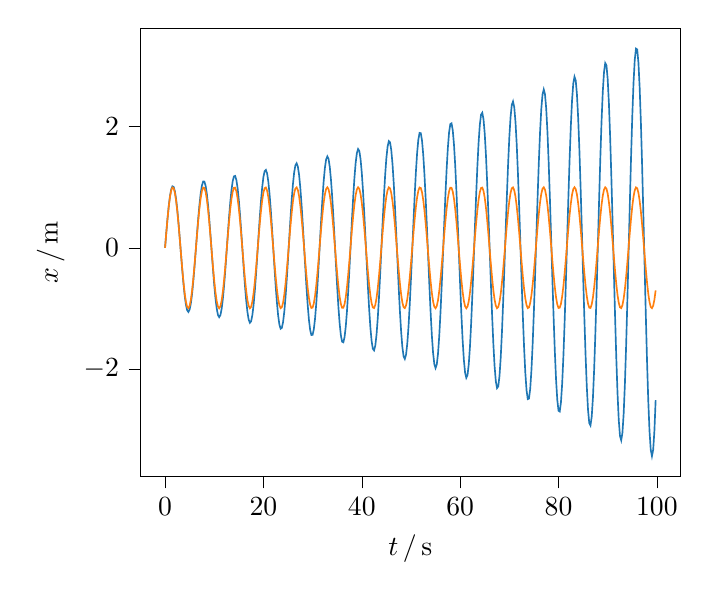
\begin{tikzpicture}

\definecolor{darkgray176}{RGB}{176,176,176}
\definecolor{darkorange25512714}{RGB}{255,127,14}
\definecolor{steelblue31119180}{RGB}{31,119,180}

\begin{axis}[
tick align=outside,
tick pos=left,
x grid style={darkgray176},
xlabel={\(\displaystyle t\,/\,\mathrm{s}\)},
xmin=-4.9875, xmax=104.7375,
xtick style={color=black},
y grid style={darkgray176},
ylabel={\(\displaystyle x\,/\,\mathrm{m}\)},
ymin=-3.7808, ymax=3.6288,
ytick style={color=black}
]
\addplot [semithick, steelblue31119180]
table {%
0 0
0.25 0.248
0.5 0.482
0.75 0.688
1 0.852
1.25 0.964
1.5 1.016
1.75 1.006
2 0.933
2.25 0.801
2.5 0.618
2.75 0.396
3 0.147
3.25 -0.112
3.5 -0.366
3.75 -0.598
4 -0.795
4.25 -0.943
4.5 -1.034
4.75 -1.061
5 -1.021
5.25 -0.918
5.5 -0.757
5.75 -0.548
6 -0.303
6.25 -0.038
6.5 0.231
6.75 0.488
7 0.715
7.25 0.9
7.5 1.029
7.75 1.096
8 1.094
8.25 1.024
8.5 0.89
8.75 0.699
9 0.464
9.25 0.198
9.5 -0.082
9.75 -0.358
10 -0.614
10.25 -0.833
10.5 -1.001
10.75 -1.109
11 -1.147
11.25 -1.115
11.5 -1.013
11.75 -0.847
12 -0.627
12.25 -0.366
12.5 -0.082
12.75 0.21
13 0.49
13.25 0.742
13.5 0.949
13.75 1.098
14 1.179
14.25 1.188
14.5 1.122
14.75 0.987
15 0.788
15.25 0.54
15.5 0.256
15.75 -0.046
16 -0.346
16.25 -0.627
16.5 -0.871
16.75 -1.061
17 -1.187
17.25 -1.24
17.5 -1.215
17.75 -1.115
18 -0.945
18.25 -0.714
18.5 -0.438
18.75 -0.132
19 0.183
19.25 0.489
19.5 0.767
19.75 0.998
20 1.169
20.25 1.268
20.5 1.288
20.75 1.229
21 1.092
21.25 0.886
21.5 0.624
21.75 0.321
22 -0.003
22.25 -0.33
22.5 -0.638
22.75 -0.908
23 -1.123
23.25 -1.27
23.5 -1.338
23.75 -1.323
24 -1.226
24.25 -1.052
24.5 -0.811
24.75 -0.518
25 -0.191
25.25 0.151
25.5 0.484
25.75 0.79
26 1.049
26.25 1.243
26.5 1.362
26.75 1.396
27 1.343
27.25 1.207
27.5 0.994
27.75 0.718
28 0.395
28.25 0.046
28.5 -0.308
28.75 -0.645
29 -0.944
29.25 -1.187
29.5 -1.356
29.75 -1.442
30 -1.439
30.25 -1.346
30.5 -1.169
30.75 -0.917
31 -0.607
31.25 -0.257
31.5 0.111
31.75 0.475
32 0.811
32.25 1.099
32.5 1.32
32.75 1.46
33 1.51
33.25 1.467
33.5 1.331
33.75 1.112
34 0.822
34.25 0.479
34.5 0.104
34.75 -0.28
35 -0.649
35.25 -0.98
35.5 -1.251
35.75 -1.447
36 -1.553
36.25 -1.563
36.5 -1.476
36.75 -1.296
37 -1.035
37.25 -0.707
37.5 -0.333
37.75 0.064
38 0.46
38.25 0.829
38.5 1.149
38.75 1.399
39 1.564
39.25 1.632
39.5 1.599
39.75 1.466
40 1.241
40.25 0.937
40.5 0.572
40.75 0.17
41 -0.245
41.25 -0.648
41.5 -1.013
41.75 -1.317
42 -1.541
42.25 -1.67
42.5 -1.696
42.75 -1.616
43 -1.435
43.25 -1.163
43.5 -0.818
43.75 -0.419
44 0.009
44.25 0.439
44.5 0.844
44.75 1.199
45 1.481
45.25 1.673
45.5 1.762
45.75 1.741
46 1.612
46.25 1.382
46.5 1.064
46.75 0.677
47 0.246
47.25 -0.203
47.5 -0.642
47.75 -1.044
48 -1.383
48.25 -1.639
48.5 -1.793
48.75 -1.837
49 -1.767
49.25 -1.586
49.5 -1.305
49.75 -0.941
50 -0.516
50.25 -0.056
50.5 0.41
50.75 0.854
51 1.247
51.25 1.565
51.5 1.787
51.75 1.899
52 1.894
52.25 1.77
52.5 1.536
52.75 1.204
53 0.795
53.25 0.334
53.5 -0.151
53.75 -0.63
54 -1.072
54.25 -1.45
54.5 -1.74
54.75 -1.923
55 -1.988
55.25 -1.929
55.5 -1.75
55.75 -1.46
56 -1.077
56.25 -0.625
56.5 -0.131
56.75 0.374
57 0.859
57.25 1.294
57.5 1.65
57.75 1.906
58 2.045
58.25 2.057
58.5 1.941
58.75 1.703
59 1.358
59.25 0.925
59.5 0.433
59.75 -0.09
60 -0.61
60.25 -1.096
60.5 -1.516
60.75 -1.845
61 -2.06
61.25 -2.149
61.5 -2.104
61.75 -1.927
62 -1.629
62.25 -1.228
62.5 -0.748
62.75 -0.218
63 0.329
63.25 0.858
63.5 1.338
63.75 1.737
64 2.03
64.25 2.199
64.5 2.232
64.75 2.125
65 1.886
65.25 1.527
65.5 1.071
65.75 0.545
66 -0.017
66.25 -0.583
66.5 -1.115
66.75 -1.582
67 -1.953
67.25 -2.204
67.5 -2.319
67.75 -2.291
68 -2.12
68.25 -1.815
68.5 -1.395
68.75 -0.886
69 -0.318
69.25 0.273
69.5 0.851
69.75 1.379
70 1.825
70.25 2.16
70.5 2.362
70.75 2.418
71 2.324
71.25 2.084
71.5 1.713
71.75 1.233
72 0.673
72.25 0.067
72.5 -0.546
72.75 -1.129
73 -1.646
73.25 -2.063
73.5 -2.354
73.75 -2.501
74 -2.492
74.25 -2.328
74.5 -2.017
74.75 -1.579
75 -1.04
75.25 -0.433
75.5 0.206
75.75 0.835
76 1.416
76.25 1.913
76.5 2.293
76.75 2.533
77 2.617
77.25 2.538
77.5 2.3
77.75 1.917
78 1.412
78.25 0.816
78.5 0.166
78.75 -0.499
79 -1.137
79.25 -1.708
79.5 -2.176
79.75 -2.512
80 -2.693
80.25 -2.707
80.5 -2.552
80.75 -2.238
81 -1.782
81.25 -1.212
81.5 -0.563
81.75 0.125
82 0.81
82.25 1.449
82.5 2.001
82.75 2.432
83 2.714
83.25 2.828
83.5 2.767
83.75 2.533
84 2.14
84.25 1.611
84.5 0.978
84.75 0.28
85 -0.44
85.25 -1.137
85.5 -1.767
85.75 -2.291
86 -2.676
86.25 -2.896
86.5 -2.937
86.75 -2.795
87 -2.478
87.25 -2.005
87.5 -1.403
87.75 -0.711
88 0.031
88.25 0.775
88.5 1.475
88.75 2.088
89 2.574
89.25 2.903
89.5 3.053
89.75 3.014
90 2.787
90.25 2.384
90.5 1.83
90.75 1.159
91 0.411
91.25 -0.367
91.5 -1.127
91.75 -1.822
92 -2.407
92.25 -2.846
92.5 -3.11
92.75 -3.182
93 -3.056
93.25 -2.739
93.5 -2.249
93.75 -1.616
94 -0.878
94.25 -0.08
94.5 0.727
94.75 1.494
95 2.173
95.25 2.721
95.5 3.102
95.75 3.292
96 3.279
96.25 3.06
96.5 2.65
96.75 2.072
97 1.361
97.25 0.561
97.5 -0.279
97.75 -1.107
98 -1.872
98.25 -2.524
98.5 -3.023
98.75 -3.337
99 -3.444
99.25 -3.338
99.5 -3.023
99.75 -2.517
};
\addplot [semithick, darkorange25512714]
table {%
0 0
0.25 0.247
0.5 0.479
0.75 0.682
1 0.841
1.25 0.949
1.5 0.997
1.75 0.984
2 0.909
2.25 0.778
2.5 0.598
2.75 0.382
3 0.141
3.25 -0.108
3.5 -0.351
3.75 -0.572
4 -0.757
4.25 -0.895
4.5 -0.978
4.75 -0.999
5 -0.959
5.25 -0.859
5.5 -0.706
5.75 -0.508
6 -0.279
6.25 -0.033
6.5 0.215
6.75 0.45
7 0.657
7.25 0.823
7.5 0.938
7.75 0.995
8 0.989
8.25 0.923
8.5 0.798
8.75 0.625
9 0.412
9.25 0.174
9.5 -0.075
9.75 -0.32
10 -0.544
10.25 -0.735
10.5 -0.88
10.75 -0.97
11 -1
11.25 -0.968
11.5 -0.875
11.75 -0.729
12 -0.537
12.25 -0.311
12.5 -0.066
12.75 0.183
13 0.42
13.25 0.632
13.5 0.804
13.75 0.926
14 0.991
14.25 0.994
14.5 0.935
14.75 0.818
15 0.65
15.25 0.442
15.5 0.206
15.75 -0.042
16 -0.288
16.25 -0.516
16.5 -0.712
16.75 -0.863
17 -0.961
17.25 -1
17.5 -0.976
17.75 -0.891
18 -0.751
18.25 -0.564
18.5 -0.342
18.75 -0.099
19 0.15
19.25 0.39
19.5 0.606
19.75 0.784
20 0.913
20.25 0.986
20.5 0.997
20.75 0.946
21 0.837
21.25 0.675
21.5 0.472
21.75 0.239
22 -0.009
22.25 -0.256
22.5 -0.487
22.75 -0.688
23 -0.846
23.25 -0.952
23.5 -0.998
23.75 -0.982
24 -0.906
24.25 -0.772
24.5 -0.591
24.75 -0.373
25 -0.132
25.25 0.117
25.5 0.359
25.75 0.579
26 0.763
26.25 0.899
26.5 0.979
26.75 0.999
27 0.956
27.25 0.854
27.5 0.699
27.75 0.501
28 0.271
28.25 0.024
28.5 -0.224
28.75 -0.458
29 -0.664
29.25 -0.828
29.5 -0.941
29.75 -0.995
30 -0.988
30.25 -0.919
30.5 -0.793
30.75 -0.618
31 -0.404
31.25 -0.165
31.5 0.084
31.75 0.328
32 0.551
32.25 0.741
32.5 0.884
32.75 0.972
33 1
33.25 0.966
33.5 0.871
33.75 0.723
34 0.529
34.25 0.303
34.5 0.057
34.75 -0.191
35 -0.428
35.25 -0.638
35.5 -0.809
35.75 -0.929
36 -0.992
36.25 -0.993
36.5 -0.932
36.75 -0.813
37 -0.644
37.25 -0.434
37.5 -0.198
37.75 0.051
38 0.296
38.25 0.523
38.5 0.718
38.75 0.868
39 0.964
39.25 1
39.5 0.974
39.75 0.887
40 0.745
40.25 0.557
40.5 0.334
40.75 0.091
41 -0.159
41.25 -0.398
41.5 -0.613
41.75 -0.789
42 -0.917
42.25 -0.987
42.5 -0.996
42.75 -0.943
43 -0.832
43.25 -0.669
43.5 -0.464
43.75 -0.23
44 0.018
44.25 0.265
44.5 0.495
44.75 0.694
45 0.851
45.25 0.954
45.5 0.999
45.75 0.981
46 0.902
46.25 0.767
46.5 0.584
46.75 0.365
47 0.124
47.25 -0.126
47.5 -0.367
47.75 -0.586
48 -0.768
48.25 -0.903
48.5 -0.981
48.75 -0.998
49 -0.954
49.25 -0.85
49.5 -0.693
49.75 -0.493
50 -0.262
50.25 -0.015
50.5 0.232
50.75 0.466
51 0.67
51.25 0.833
51.5 0.944
51.75 0.996
52 0.987
52.25 0.916
52.5 0.788
52.75 0.611
53 0.396
53.25 0.156
53.5 -0.093
53.75 -0.336
54 -0.559
54.25 -0.747
54.5 -0.888
54.75 -0.974
55 -1
55.25 -0.963
55.5 -0.867
55.75 -0.716
56 -0.522
56.25 -0.294
56.5 -0.049
56.75 0.2
57 0.436
57.25 0.645
57.5 0.814
57.75 0.933
58 0.993
58.25 0.991
58.5 0.928
58.75 0.808
59 0.637
59.25 0.426
59.5 0.189
59.75 -0.06
60 -0.305
60.25 -0.531
60.5 -0.724
60.75 -0.872
61 -0.966
61.25 -1
61.5 -0.972
61.75 -0.883
62 -0.739
62.25 -0.55
62.5 -0.326
62.75 -0.082
63 0.167
63.25 0.406
63.5 0.62
63.75 0.794
64 0.92
64.25 0.988
64.5 0.995
64.75 0.94
65 0.827
65.25 0.662
65.5 0.456
65.75 0.222
66 -0.027
66.25 -0.273
66.5 -0.503
66.75 -0.701
67 -0.856
67.25 -0.957
67.5 -0.999
67.75 -0.979
68 -0.898
68.25 -0.761
68.5 -0.577
68.75 -0.357
69 -0.115
69.25 0.135
69.5 0.376
69.75 0.593
70 0.774
70.25 0.907
70.5 0.983
70.75 0.998
71 0.951
71.25 0.845
71.5 0.686
71.75 0.485
72 0.254
72.25 0.007
72.5 -0.241
72.75 -0.474
73 -0.677
73.25 -0.838
73.5 -0.947
73.75 -0.997
74 -0.985
74.25 -0.912
74.5 -0.782
74.75 -0.604
75 -0.388
75.25 -0.148
75.5 0.102
75.75 0.345
76 0.566
76.25 0.752
76.5 0.892
76.75 0.976
77 1
77.25 0.961
77.5 0.862
77.75 0.71
78 0.514
78.25 0.286
78.5 0.04
78.75 -0.209
79 -0.444
79.25 -0.652
79.5 -0.819
79.75 -0.936
80 -0.994
80.25 -0.99
80.5 -0.925
80.75 -0.802
81 -0.63
81.25 -0.418
81.5 -0.18
81.75 0.069
82 0.313
82.25 0.538
82.5 0.73
82.75 0.877
83 0.968
83.25 1
83.5 0.969
83.75 0.879
84 0.733
84.25 0.542
84.5 0.317
84.75 0.073
85 -0.176
85.25 -0.414
85.5 -0.626
85.75 -0.8
86 -0.923
86.25 -0.99
86.5 -0.994
86.75 -0.937
87 -0.822
87.25 -0.655
87.5 -0.448
87.75 -0.213
88 0.035
88.25 0.282
88.5 0.51
88.75 0.707
89 0.86
89.25 0.96
89.5 0.999
89.75 0.977
90 0.894
90.25 0.755
90.5 0.57
90.75 0.349
91 0.106
91.25 -0.143
91.5 -0.384
91.75 -0.6
92 -0.779
92.25 -0.91
92.5 -0.984
92.75 -0.997
93 -0.948
93.25 -0.84
93.5 -0.68
93.75 -0.477
94 -0.245
94.25 0.002
94.5 0.25
94.75 0.481
95 0.683
95.25 0.843
95.5 0.95
95.75 0.998
96 0.984
96.25 0.908
96.5 0.777
96.75 0.597
97 0.38
97.25 0.139
97.5 -0.11
97.75 -0.353
98 -0.573
98.25 -0.758
98.5 -0.896
98.75 -0.978
99 -0.999
99.25 -0.958
99.5 -0.858
99.75 -0.704
};
\end{axis}

\end{tikzpicture}

            \end{adjustbox}
            \caption{Displacement against time}
        \end{subfigure}
        \hfill
        \begin{subfigure}[h]{0.48\linewidth}
            \begin{adjustbox}{width=\linewidth}
            % This file was created with tikzplotlib v0.10.1.
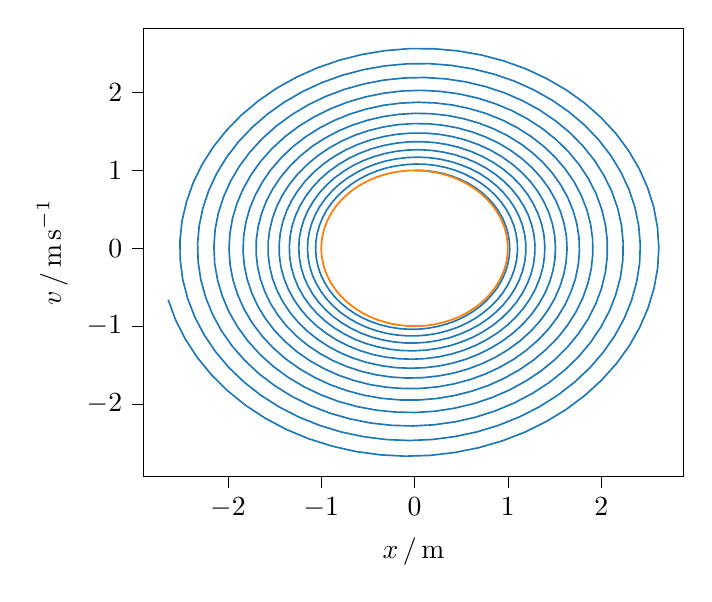
\begin{tikzpicture}

\definecolor{darkgray176}{RGB}{176,176,176}
\definecolor{darkorange25512714}{RGB}{255,127,14}
\definecolor{steelblue31119180}{RGB}{31,119,180}

\begin{axis}[
tick align=outside,
tick pos=left,
x grid style={darkgray176},
xlabel={\(\displaystyle x\,/\,\mathrm{m}\)},
xmin=-2.90285, xmax=2.87985,
xtick style={color=black},
y grid style={darkgray176},
ylabel={\(\displaystyle v\,/\,\mathrm{m\, s^{-1}}\)},
ymin=-2.93065, ymax=2.82565,
ytick style={color=black}
]
\addplot [semithick, steelblue31119180]
table {%
0 1
0.1 0.998
0.199 0.985
0.297 0.963
0.391 0.931
0.482 0.889
0.569 0.839
0.65 0.78
0.724 0.713
0.792 0.639
0.852 0.558
0.903 0.471
0.946 0.38
0.979 0.284
1.003 0.186
1.016 0.085
1.02 -0.017
1.013 -0.118
0.996 -0.219
0.969 -0.318
0.933 -0.414
0.887 -0.507
0.831 -0.594
0.768 -0.676
0.697 -0.751
0.618 -0.818
0.533 -0.878
0.443 -0.929
0.348 -0.971
0.249 -1.003
0.147 -1.026
0.044 -1.038
-0.06 -1.04
-0.163 -1.031
-0.266 -1.012
-0.366 -0.983
-0.462 -0.944
-0.554 -0.896
-0.641 -0.838
-0.721 -0.772
-0.795 -0.698
-0.861 -0.617
-0.918 -0.529
-0.966 -0.436
-1.005 -0.339
-1.034 -0.237
-1.052 -0.133
-1.06 -0.028
-1.058 0.078
-1.045 0.184
-1.021 0.288
-0.987 0.389
-0.944 0.487
-0.89 0.58
-0.828 0.667
-0.757 0.748
-0.678 0.822
-0.593 0.888
-0.501 0.945
-0.404 0.993
-0.303 1.031
-0.198 1.058
-0.092 1.075
0.016 1.082
0.124 1.078
0.231 1.063
0.336 1.037
0.438 1.001
0.536 0.954
0.629 0.898
0.715 0.833
0.795 0.76
0.867 0.678
0.931 0.59
0.985 0.495
1.029 0.396
1.064 0.292
1.088 0.185
1.101 0.076
1.103 -0.034
1.094 -0.145
1.074 -0.254
1.043 -0.36
1.002 -0.464
0.951 -0.563
0.89 -0.656
0.82 -0.743
0.741 -0.823
0.655 -0.896
0.562 -0.959
0.464 -1.013
0.36 -1.056
0.253 -1.09
0.143 -1.112
0.031 -1.124
-0.082 -1.124
-0.194 -1.113
-0.304 -1.091
-0.411 -1.058
-0.515 -1.014
-0.614 -0.96
-0.707 -0.896
-0.793 -0.824
-0.871 -0.742
-0.941 -0.653
-1.001 -0.558
-1.052 -0.456
-1.093 -0.35
-1.122 -0.24
-1.14 -0.127
-1.147 -0.013
-1.143 0.102
-1.127 0.216
-1.1 0.328
-1.062 0.437
-1.013 0.542
-0.953 0.642
-0.884 0.736
-0.807 0.822
-0.72 0.901
-0.627 0.97
-0.527 1.031
-0.421 1.081
-0.311 1.12
-0.197 1.148
-0.082 1.165
0.035 1.17
0.152 1.164
0.267 1.146
0.381 1.116
0.49 1.075
0.595 1.024
0.695 0.962
0.787 0.89
0.872 0.809
0.949 0.72
1.016 0.623
1.073 0.52
1.12 0.411
1.155 0.299
1.179 0.182
1.192 0.064
1.192 -0.055
1.181 -0.174
1.157 -0.292
1.122 -0.407
1.076 -0.518
1.019 -0.624
0.952 -0.724
0.874 -0.818
0.788 -0.903
0.694 -0.98
0.593 -1.046
0.485 -1.103
0.373 -1.149
0.256 -1.183
0.136 -1.206
0.015 -1.216
-0.106 -1.215
-0.227 -1.201
-0.346 -1.175
-0.462 -1.138
-0.573 -1.089
-0.679 -1.029
-0.779 -0.958
-0.871 -0.878
-0.954 -0.789
-1.028 -0.692
-1.092 -0.587
-1.145 -0.477
-1.187 -0.361
-1.217 -0.241
-1.235 -0.119
-1.241 0.005
-1.235 0.129
-1.215 0.252
-1.184 0.373
-1.141 0.49
-1.086 0.603
-1.021 0.71
-0.945 0.81
-0.859 0.903
-0.764 0.986
-0.662 1.06
-0.553 1.124
-0.438 1.176
-0.318 1.217
-0.195 1.246
-0.069 1.262
0.057 1.266
0.183 1.257
0.308 1.235
0.43 1.202
0.548 1.156
0.661 1.098
0.767 1.029
0.866 0.95
0.957 0.861
1.038 0.763
1.109 0.658
1.169 0.545
1.218 0.427
1.254 0.304
1.279 0.178
1.29 0.05
1.288 -0.079
1.274 -0.208
1.247 -0.335
1.207 -0.458
1.155 -0.578
1.092 -0.692
1.017 -0.799
0.932 -0.899
0.838 -0.99
0.735 -1.071
0.624 -1.142
0.507 -1.201
0.384 -1.249
0.258 -1.284
0.128 -1.307
-0.003 -1.316
-0.135 -1.313
-0.265 -1.296
-0.394 -1.266
-0.518 -1.224
-0.638 -1.169
-0.751 -1.102
-0.858 -1.024
-0.956 -0.936
-1.045 -0.838
-1.123 -0.732
-1.191 -0.618
-1.247 -0.497
-1.29 -0.371
-1.321 -0.241
-1.338 -0.109
-1.342 0.025
-1.333 0.159
-1.311 0.292
-1.275 0.422
-1.226 0.549
-1.165 0.67
-1.092 0.785
-1.009 0.892
-0.914 0.99
-0.811 1.079
-0.699 1.158
-0.58 1.225
-0.454 1.28
-0.324 1.322
-0.191 1.351
-0.055 1.367
0.082 1.369
0.219 1.357
0.353 1.332
0.484 1.293
0.611 1.241
0.732 1.177
0.846 1.101
0.952 1.014
1.049 0.916
1.135 0.809
1.21 0.694
1.273 0.571
1.324 0.442
1.362 0.309
1.386 0.172
1.396 0.033
1.392 -0.107
1.375 -0.245
1.343 -0.382
1.298 -0.515
1.24 -0.644
1.17 -0.766
1.087 -0.881
0.994 -0.988
0.89 -1.085
0.777 -1.171
0.656 -1.246
0.529 -1.308
0.395 -1.358
0.258 -1.394
0.117 -1.416
-0.025 -1.424
-0.167 -1.418
-0.308 -1.398
-0.446 -1.364
-0.58 -1.316
-0.709 -1.254
-0.831 -1.18
-0.944 -1.094
-1.049 -0.997
-1.144 -0.89
-1.227 -0.773
-1.298 -0.649
-1.356 -0.517
-1.401 -0.381
-1.432 -0.24
-1.449 -0.096
-1.451 0.049
-1.439 0.194
-1.413 0.337
-1.372 0.478
-1.317 0.614
-1.249 0.744
-1.169 0.867
-1.076 0.981
-0.973 1.086
-0.859 1.181
-0.737 1.264
-0.607 1.334
-0.471 1.392
-0.329 1.435
-0.184 1.465
-0.037 1.479
0.111 1.479
0.258 1.465
0.404 1.435
0.545 1.391
0.681 1.333
0.811 1.262
0.933 1.178
1.046 1.081
1.149 0.974
1.241 0.857
1.32 0.731
1.386 0.597
1.439 0.457
1.478 0.312
1.501 0.164
1.51 0.013
1.504 -0.138
1.483 -0.288
1.447 -0.435
1.396 -0.579
1.331 -0.717
1.253 -0.848
1.162 -0.971
1.059 -1.085
0.945 -1.188
0.822 -1.279
0.69 -1.358
0.551 -1.424
0.406 -1.475
0.256 -1.512
0.104 -1.534
-0.05 -1.54
-0.204 -1.532
-0.356 -1.507
-0.505 -1.468
-0.649 -1.414
-0.787 -1.346
-0.918 -1.264
-1.039 -1.169
-1.151 -1.062
-1.251 -0.944
-1.339 -0.817
-1.414 -0.681
-1.475 -0.538
-1.522 -0.389
-1.553 -0.236
-1.569 -0.08
-1.569 0.077
-1.553 0.233
-1.522 0.388
-1.476 0.539
-1.415 0.685
-1.339 0.825
-1.25 0.957
-1.148 1.079
-1.035 1.191
-0.91 1.292
-0.777 1.379
-0.635 1.454
-0.486 1.513
-0.333 1.558
-0.175 1.588
-0.016 1.601
0.144 1.599
0.303 1.58
0.46 1.546
0.612 1.496
0.758 1.431
0.898 1.352
1.028 1.259
1.149 1.153
1.259 1.035
1.356 0.907
1.44 0.769
1.509 0.623
1.564 0.471
1.603 0.314
1.627 0.153
1.634 -0.01
1.624 -0.174
1.599 -0.336
1.557 -0.494
1.5 -0.649
1.428 -0.797
1.341 -0.938
1.241 -1.07
1.128 -1.191
1.003 -1.301
0.868 -1.398
0.724 -1.481
0.572 -1.55
0.415 -1.603
0.252 -1.64
0.087 -1.661
-0.079 -1.666
-0.245 -1.654
-0.409 -1.625
-0.57 -1.58
-0.725 -1.519
-0.873 -1.443
-1.013 -1.352
-1.143 -1.248
-1.262 -1.13
-1.369 -1.001
-1.462 -0.862
-1.541 -0.714
-1.604 -0.558
-1.652 -0.396
-1.683 -0.23
-1.698 -0.061
-1.696 0.108
-1.676 0.278
-1.64 0.445
-1.588 0.607
-1.519 0.764
-1.435 0.914
-1.336 1.055
-1.224 1.186
-1.1 1.306
-0.964 1.412
-0.818 1.505
-0.663 1.583
-0.502 1.645
-0.335 1.691
-0.164 1.721
0.009 1.733
0.182 1.728
0.354 1.705
0.522 1.665
0.686 1.609
0.844 1.536
0.993 1.448
1.133 1.345
1.261 1.229
1.378 1.1
1.481 0.959
1.569 0.809
1.642 0.65
1.699 0.484
1.739 0.313
1.762 0.139
1.767 -0.038
1.754 -0.214
1.724 -0.389
1.676 -0.56
1.612 -0.726
1.531 -0.886
1.435 -1.037
1.325 -1.177
1.2 -1.307
1.064 -1.424
0.916 -1.526
0.759 -1.614
0.594 -1.686
0.422 -1.741
0.246 -1.779
0.067 -1.799
-0.113 -1.801
-0.292 -1.785
-0.469 -1.752
-0.642 -1.7
-0.809 -1.632
-0.968 -1.547
-1.118 -1.447
-1.257 -1.331
-1.383 -1.202
-1.497 -1.061
-1.595 -0.909
-1.678 -0.747
-1.744 -0.578
-1.793 -0.402
-1.824 -0.222
-1.838 -0.039
-1.832 0.145
-1.809 0.328
-1.767 0.508
-1.707 0.683
-1.63 0.852
-1.537 1.013
-1.428 1.164
-1.305 1.304
-1.168 1.431
-1.019 1.544
-0.86 1.642
-0.691 1.724
-0.516 1.788
-0.334 1.836
-0.149 1.864
0.038 1.875
0.225 1.866
0.41 1.839
0.592 1.793
0.768 1.73
0.937 1.649
1.097 1.551
1.247 1.437
1.384 1.309
1.508 1.168
1.617 1.014
1.711 0.85
1.787 0.677
1.846 0.496
1.886 0.311
1.908 0.121
1.91 -0.07
1.894 -0.26
1.858 -0.449
1.804 -0.633
1.732 -0.812
1.642 -0.983
1.536 -1.145
1.413 -1.295
1.277 -1.433
1.127 -1.557
0.966 -1.666
0.795 -1.759
0.615 -1.834
0.429 -1.89
0.237 -1.929
0.044 -1.948
-0.151 -1.947
-0.345 -1.927
-0.536 -1.888
-0.722 -1.829
-0.901 -1.753
-1.072 -1.658
-1.232 -1.547
-1.381 -1.42
-1.516 -1.278
-1.636 -1.124
-1.74 -0.958
-1.827 -0.781
-1.896 -0.597
-1.946 -0.406
-1.977 -0.21
-1.988 -0.012
-1.979 0.187
-1.951 0.384
-1.903 0.578
-1.835 0.767
-1.75 0.948
-1.646 1.121
-1.526 1.282
-1.39 1.432
-1.24 1.567
-1.077 1.687
-0.903 1.79
-0.72 1.876
-0.529 1.943
-0.332 1.991
-0.131 2.02
0.071 2.028
0.274 2.015
0.474 1.983
0.669 1.931
0.859 1.859
1.041 1.769
1.212 1.66
1.372 1.535
1.518 1.394
1.65 1.239
1.766 1.071
1.864 0.892
1.944 0.703
2.004 0.507
2.045 0.306
2.065 0.1
2.065 -0.106
2.044 -0.312
2.003 -0.516
1.941 -0.715
1.86 -0.907
1.76 -1.09
1.642 -1.264
1.508 -1.425
1.358 -1.572
1.194 -1.703
1.018 -1.819
0.831 -1.916
0.635 -1.994
0.433 -2.052
0.226 -2.091
0.015 -2.108
-0.195 -2.104
-0.405 -2.079
-0.61 -2.034
-0.811 -1.968
-1.003 -1.882
-1.186 -1.777
-1.358 -1.654
-1.516 -1.514
-1.66 -1.359
-1.787 -1.189
-1.897 -1.008
-1.989 -0.816
-2.06 -0.615
-2.111 -0.407
-2.142 -0.195
-2.15 0.019
-2.138 0.234
-2.104 0.447
-2.048 0.656
-1.973 0.859
-1.877 1.054
-1.762 1.239
-1.629 1.412
-1.48 1.571
-1.316 1.715
-1.138 1.843
-0.948 1.952
-0.748 2.042
-0.54 2.111
-0.327 2.16
-0.109 2.187
0.11 2.193
0.329 2.176
0.544 2.138
0.755 2.078
0.959 1.998
1.154 1.897
1.338 1.777
1.509 1.638
1.665 1.484
1.805 1.313
1.927 1.13
2.03 0.934
2.114 0.729
2.176 0.516
2.217 0.297
2.235 0.075
2.232 -0.149
2.206 -0.371
2.157 -0.591
2.088 -0.805
1.997 -1.011
1.886 -1.208
1.756 -1.394
1.607 -1.566
1.443 -1.723
1.264 -1.862
1.071 -1.984
0.868 -2.086
0.655 -2.168
0.435 -2.228
0.21 -2.266
-0.017 -2.281
-0.245 -2.273
-0.471 -2.243
-0.693 -2.19
-0.909 -2.116
-1.115 -2.02
-1.312 -1.903
-1.495 -1.767
-1.665 -1.613
-1.817 -1.443
-1.953 -1.258
-2.069 -1.06
-2.164 -0.85
-2.238 -0.632
-2.29 -0.406
-2.319 -0.177
-2.325 0.056
-2.308 0.288
-2.268 0.518
-2.205 0.743
-2.12 0.962
-2.013 1.171
-1.886 1.369
-1.739 1.554
-1.575 1.724
-1.395 1.877
-1.201 2.012
-0.994 2.127
-0.776 2.221
-0.55 2.293
-0.318 2.342
-0.083 2.368
0.155 2.371
0.391 2.349
0.624 2.304
0.851 2.236
1.07 2.146
1.279 2.033
1.476 1.9
1.658 1.748
1.825 1.578
1.973 1.392
2.103 1.191
2.211 0.978
2.298 0.755
2.362 0.523
2.402 0.286
2.419 0.045
2.411 -0.197
2.379 -0.437
2.324 -0.674
2.245 -0.905
2.143 -1.127
2.02 -1.338
1.876 -1.537
1.713 -1.72
1.533 -1.887
1.336 -2.036
1.126 -2.164
0.904 -2.271
0.673 -2.356
0.434 -2.417
0.19 -2.455
-0.056 -2.468
-0.302 -2.456
-0.546 -2.419
-0.785 -2.359
-1.017 -2.274
-1.239 -2.167
-1.45 -2.038
-1.646 -1.888
-1.826 -1.719
-1.989 -1.532
-2.132 -1.329
-2.254 -1.113
-2.354 -0.885
-2.431 -0.647
-2.484 -0.403
-2.511 -0.153
-2.514 0.098
-2.492 0.349
-2.444 0.597
-2.373 0.84
-2.277 1.075
-2.158 1.3
-2.017 1.512
-1.856 1.71
-1.676 1.891
-1.479 2.054
-1.266 2.197
-1.04 2.318
-0.803 2.416
-0.558 2.49
-0.306 2.539
-0.051 2.564
0.206 2.562
0.461 2.535
0.712 2.483
0.956 2.406
1.192 2.304
1.416 2.179
1.627 2.032
1.822 1.865
1.999 1.678
2.157 1.474
2.293 1.255
2.407 1.022
2.497 0.779
2.563 0.528
2.603 0.27
2.617 0.009
2.605 -0.252
2.566 -0.512
2.502 -0.767
2.413 -1.015
2.3 -1.254
2.163 -1.481
2.004 -1.693
1.825 -1.889
1.627 -2.067
1.412 -2.224
1.183 -2.36
0.941 -2.472
0.689 -2.56
0.43 -2.622
0.166 -2.659
-0.101 -2.669
-0.367 -2.652
-0.63 -2.609
-0.888 -2.539
-1.137 -2.444
-1.376 -2.325
-1.601 -2.181
-1.811 -2.016
-2.003 -1.83
-2.176 -1.625
-2.328 -1.403
-2.456 -1.167
-2.561 -0.919
-2.64 -0.661
};
\addplot [semithick, darkorange25512714]
table {%
0 1
0.1 0.995
0.199 0.98
0.296 0.955
0.389 0.921
0.479 0.878
0.565 0.825
0.644 0.765
0.717 0.697
0.783 0.622
0.841 0.54
0.891 0.454
0.932 0.362
0.964 0.267
0.985 0.17
0.997 0.071
1 -0.029
0.992 -0.129
0.974 -0.227
0.946 -0.323
0.909 -0.416
0.863 -0.505
0.808 -0.589
0.746 -0.666
0.675 -0.737
0.598 -0.801
0.516 -0.857
0.427 -0.904
0.335 -0.942
0.239 -0.971
0.141 -0.99
0.042 -0.999
-0.058 -0.998
-0.158 -0.987
-0.256 -0.967
-0.351 -0.936
-0.443 -0.897
-0.53 -0.848
-0.612 -0.791
-0.688 -0.726
-0.757 -0.654
-0.818 -0.575
-0.872 -0.49
-0.916 -0.401
-0.952 -0.307
-0.978 -0.211
-0.994 -0.112
-1 -0.012
-0.996 0.087
-0.982 0.187
-0.959 0.284
-0.926 0.378
-0.883 0.469
-0.832 0.554
-0.773 0.635
-0.706 0.709
-0.631 0.776
-0.551 0.835
-0.465 0.886
-0.374 0.927
-0.279 0.96
-0.182 0.983
-0.083 0.997
0.017 1
0.117 0.993
0.215 0.977
0.312 0.95
0.405 0.914
0.494 0.869
0.578 0.816
0.657 0.754
0.729 0.685
0.794 0.608
0.85 0.526
0.899 0.439
0.938 0.347
0.968 0.251
0.988 0.153
0.999 0.054
0.999 -0.046
0.989 -0.146
0.97 -0.244
0.941 -0.339
0.902 -0.431
0.855 -0.519
0.798 -0.602
0.734 -0.679
0.663 -0.749
0.585 -0.811
0.501 -0.865
0.412 -0.911
0.319 -0.948
0.223 -0.975
0.124 -0.992
0.025 -1
-0.075 -0.997
-0.174 -0.985
-0.272 -0.962
-0.366 -0.93
-0.458 -0.889
-0.544 -0.839
-0.625 -0.781
-0.7 -0.714
-0.768 -0.641
-0.828 -0.561
-0.88 -0.476
-0.923 -0.385
-0.957 -0.291
-0.981 -0.194
-0.995 -0.095
-1 0.004
-0.995 0.104
-0.979 0.203
-0.954 0.3
-0.919 0.393
-0.875 0.483
-0.823 0.568
-0.762 0.648
-0.694 0.72
-0.618 0.786
-0.537 0.844
-0.45 0.893
-0.358 0.934
-0.263 0.965
-0.166 0.986
-0.066 0.998
0.034 0.999
0.133 0.991
0.232 0.973
0.327 0.945
0.42 0.907
0.509 0.861
0.592 0.806
0.67 0.743
0.74 0.672
0.804 0.595
0.859 0.512
0.906 0.423
0.944 0.331
0.972 0.235
0.991 0.137
0.999 0.037
0.998 -0.063
0.987 -0.162
0.966 -0.26
0.935 -0.355
0.895 -0.446
0.846 -0.534
0.788 -0.615
0.723 -0.691
0.65 -0.76
0.571 -0.821
0.486 -0.874
0.397 -0.918
0.303 -0.953
0.206 -0.978
0.108 -0.994
0.008 -1
-0.092 -0.996
-0.191 -0.982
-0.288 -0.958
-0.382 -0.924
-0.472 -0.881
-0.558 -0.83
-0.638 -0.77
-0.712 -0.702
-0.778 -0.628
-0.837 -0.547
-0.888 -0.461
-0.929 -0.37
-0.961 -0.275
-0.984 -0.178
-0.997 -0.079
-1 0.021
-0.993 0.121
-0.976 0.219
-0.949 0.316
-0.913 0.409
-0.867 0.498
-0.813 0.582
-0.751 0.66
-0.681 0.732
-0.605 0.796
-0.522 0.853
-0.435 0.901
-0.342 0.94
-0.247 0.969
-0.149 0.989
-0.05 0.999
0.05 0.999
0.15 0.989
0.248 0.969
0.343 0.939
0.435 0.9
0.523 0.852
0.606 0.796
0.682 0.731
0.752 0.66
0.814 0.581
0.868 0.497
0.913 0.408
0.949 0.315
0.976 0.219
0.993 0.12
1 0.02
0.997 -0.08
0.984 -0.179
0.961 -0.276
0.929 -0.371
0.887 -0.461
0.837 -0.548
0.778 -0.629
0.711 -0.703
0.637 -0.771
0.557 -0.83
0.472 -0.882
0.381 -0.924
0.287 -0.958
0.19 -0.982
0.091 -0.996
-0.009 -1
-0.109 -0.994
-0.207 -0.978
-0.304 -0.953
-0.398 -0.918
-0.487 -0.873
-0.572 -0.82
-0.651 -0.759
-0.723 -0.69
-0.789 -0.615
-0.846 -0.533
-0.895 -0.446
-0.935 -0.354
-0.966 -0.259
-0.987 -0.161
-0.998 -0.062
-0.999 0.038
-0.99 0.138
-0.972 0.236
-0.943 0.332
-0.906 0.424
-0.859 0.512
-0.803 0.596
-0.74 0.673
-0.669 0.743
-0.591 0.806
-0.508 0.861
-0.419 0.908
-0.327 0.945
-0.231 0.973
-0.132 0.991
-0.033 0.999
0.067 0.998
0.166 0.986
0.264 0.964
0.359 0.933
0.45 0.893
0.537 0.843
0.619 0.786
0.694 0.72
0.763 0.647
0.823 0.568
0.876 0.483
0.92 0.393
0.954 0.299
0.979 0.202
0.995 0.103
1 0.004
0.995 -0.096
0.981 -0.195
0.956 -0.292
0.922 -0.386
0.879 -0.476
0.827 -0.562
0.767 -0.642
0.699 -0.715
0.624 -0.781
0.543 -0.84
0.457 -0.89
0.366 -0.931
0.271 -0.963
0.173 -0.985
0.074 -0.997
-0.026 -1
-0.125 -0.992
-0.224 -0.975
-0.32 -0.947
-0.413 -0.911
-0.502 -0.865
-0.586 -0.811
-0.664 -0.748
-0.735 -0.678
-0.799 -0.601
-0.855 -0.519
-0.903 -0.431
-0.941 -0.338
-0.97 -0.243
-0.989 -0.145
-0.999 -0.045
-0.998 0.055
-0.988 0.154
-0.968 0.252
-0.938 0.347
-0.898 0.439
-0.85 0.527
-0.793 0.609
-0.728 0.685
-0.656 0.754
-0.578 0.816
-0.493 0.87
-0.404 0.915
-0.311 0.951
-0.214 0.977
-0.116 0.993
-0.016 1
0.084 0.996
0.183 0.983
0.28 0.96
0.375 0.927
0.465 0.885
0.551 0.834
0.632 0.775
0.706 0.708
0.773 0.634
0.833 0.554
0.884 0.468
0.926 0.377
0.959 0.283
0.983 0.186
0.996 0.087
1 -0.013
0.994 -0.113
0.977 -0.212
0.951 -0.308
0.916 -0.402
0.871 -0.491
0.818 -0.576
0.756 -0.654
0.687 -0.727
0.611 -0.792
0.529 -0.849
0.442 -0.897
0.35 -0.937
0.255 -0.967
0.157 -0.988
0.057 -0.998
-0.042 -0.999
-0.142 -0.99
-0.24 -0.971
-0.336 -0.942
-0.428 -0.904
-0.516 -0.856
-0.599 -0.801
-0.676 -0.737
-0.746 -0.666
-0.809 -0.588
-0.864 -0.504
-0.91 -0.415
-0.947 -0.322
-0.974 -0.226
-0.992 -0.128
-1 -0.028
-0.997 0.072
-0.985 0.171
-0.963 0.268
-0.932 0.363
-0.891 0.454
-0.841 0.541
-0.783 0.622
-0.717 0.697
-0.644 0.765
-0.564 0.826
-0.479 0.878
-0.389 0.921
-0.295 0.956
-0.198 0.98
-0.099 0.995
0.001 1
0.101 0.995
0.2 0.98
0.296 0.955
0.39 0.921
0.48 0.877
0.565 0.825
0.645 0.764
0.718 0.696
0.784 0.621
0.842 0.54
0.892 0.453
0.932 0.362
0.964 0.267
0.986 0.169
0.998 0.07
1 -0.03
0.992 -0.13
0.974 -0.228
0.946 -0.324
0.909 -0.417
0.863 -0.506
0.808 -0.589
0.745 -0.667
0.675 -0.738
0.598 -0.802
0.515 -0.857
0.427 -0.904
0.334 -0.943
0.238 -0.971
0.14 -0.99
0.041 -0.999
-0.059 -0.998
-0.159 -0.987
-0.256 -0.967
-0.352 -0.936
-0.443 -0.896
-0.531 -0.848
-0.613 -0.79
-0.688 -0.725
-0.757 -0.653
-0.819 -0.574
-0.872 -0.489
-0.917 -0.4
-0.952 -0.306
-0.978 -0.21
-0.994 -0.111
-1 -0.012
-0.996 0.088
-0.982 0.187
-0.959 0.285
-0.925 0.379
-0.883 0.469
-0.832 0.555
-0.772 0.635
-0.705 0.709
-0.631 0.776
-0.55 0.835
-0.464 0.886
-0.373 0.928
-0.279 0.96
-0.181 0.983
-0.082 0.997
0.018 1
0.117 0.993
0.216 0.976
0.312 0.95
0.406 0.914
0.495 0.869
0.579 0.815
0.658 0.753
0.73 0.684
0.794 0.608
0.851 0.525
0.899 0.438
0.938 0.346
0.968 0.25
0.988 0.152
0.999 0.053
0.999 -0.047
0.989 -0.146
0.97 -0.244
0.94 -0.34
0.902 -0.432
0.854 -0.52
0.798 -0.603
0.734 -0.679
0.662 -0.749
0.584 -0.812
0.5 -0.866
0.411 -0.911
0.318 -0.948
0.222 -0.975
0.124 -0.992
0.024 -1
-0.076 -0.997
-0.175 -0.985
-0.273 -0.962
-0.367 -0.93
-0.458 -0.889
-0.545 -0.839
-0.626 -0.78
-0.701 -0.714
-0.768 -0.64
-0.828 -0.56
-0.88 -0.475
-0.923 -0.385
-0.957 -0.29
-0.981 -0.193
-0.996 -0.095
-1 0.005
-0.994 0.105
-0.979 0.204
-0.954 0.301
-0.919 0.394
-0.875 0.484
-0.822 0.569
-0.761 0.648
-0.693 0.721
-0.617 0.787
-0.536 0.844
-0.449 0.894
-0.357 0.934
-0.262 0.965
-0.165 0.986
-0.065 0.998
0.035 0.999
0.134 0.991
0.232 0.973
0.328 0.945
0.421 0.907
0.509 0.861
0.593 0.805
0.67 0.742
0.741 0.672
0.804 0.594
0.86 0.511
0.906 0.423
0.944 0.33
0.972 0.234
0.991 0.136
0.999 0.036
0.998 -0.064
0.987 -0.163
0.965 -0.261
0.935 -0.356
0.894 -0.447
0.845 -0.534
0.788 -0.616
0.722 -0.692
0.65 -0.76
0.57 -0.821
0.486 -0.874
0.396 -0.918
0.302 -0.953
0.206 -0.979
0.107 -0.994
0.007 -1
-0.093 -0.996
-0.192 -0.981
-0.289 -0.957
-0.383 -0.924
-0.473 -0.881
-0.559 -0.829
-0.639 -0.769
-0.712 -0.702
-0.779 -0.627
-0.838 -0.546
-0.888 -0.46
-0.929 -0.369
-0.962 -0.274
-0.984 -0.177
-0.997 -0.078
-1 0.022
-0.993 0.122
-0.975 0.22
-0.949 0.317
-0.912 0.41
-0.867 0.499
-0.813 0.583
-0.75 0.661
-0.681 0.733
-0.604 0.797
-0.522 0.853
-0.434 0.901
-0.342 0.94
-0.246 0.969
-0.148 0.989
-0.049 0.999
0.051 0.999
0.151 0.989
0.249 0.969
0.344 0.939
0.436 0.9
0.524 0.852
0.606 0.795
0.683 0.731
0.752 0.659
0.814 0.581
0.868 0.496
0.913 0.407
0.949 0.314
0.976 0.218
0.993 0.119
1 0.019
0.997 -0.08
0.984 -0.18
0.961 -0.277
0.928 -0.371
0.887 -0.462
0.836 -0.548
0.777 -0.629
0.711 -0.704
0.637 -0.771
0.557 -0.831
0.471 -0.882
0.38 -0.925
0.286 -0.958
0.189 -0.982
0.09 -0.996
-0.01 -1
-0.11 -0.994
-0.208 -0.978
-0.305 -0.952
-0.398 -0.917
-0.488 -0.873
-0.573 -0.82
-0.652 -0.759
-0.724 -0.69
-0.789 -0.614
-0.847 -0.532
-0.896 -0.445
-0.936 -0.353
-0.966 -0.258
-0.987 -0.16
-0.998 -0.061
-0.999 0.039
-0.99 0.138
-0.972 0.237
-0.943 0.332
-0.905 0.425
-0.858 0.513
-0.803 0.596
-0.739 0.674
-0.668 0.744
-0.591 0.807
-0.507 0.862
-0.419 0.908
-0.326 0.945
-0.23 0.973
-0.131 0.991
-0.032 0.999
0.068 0.998
0.167 0.986
0.265 0.964
0.36 0.933
0.451 0.892
0.538 0.843
0.62 0.785
0.695 0.719
0.763 0.646
0.824 0.567
0.876 0.482
0.92 0.392
0.955 0.298
0.98 0.201
0.995 0.102
1 0.003
0.995 -0.097
0.981 -0.196
0.956 -0.293
0.922 -0.387
0.879 -0.477
0.827 -0.562
0.767 -0.642
0.699 -0.716
0.624 -0.782
0.543 -0.84
0.456 -0.89
0.365 -0.931
0.27 -0.963
0.173 -0.985
0.073 -0.997
-0.027 -1
-0.126 -0.992
-0.225 -0.974
-0.321 -0.947
-0.414 -0.91
-0.503 -0.865
-0.586 -0.81
-0.664 -0.747
-0.736 -0.677
-0.8 -0.601
-0.856 -0.518
-0.903 -0.43
-0.941 -0.337
-0.97 -0.242
-0.99 -0.144
-0.999 -0.044
-0.998 0.056
-0.988 0.155
-0.967 0.253
-0.937 0.348
-0.898 0.44
-0.85 0.528
-0.793 0.61
-0.728 0.686
-0.656 0.755
-0.577 0.817
-0.493 0.87
-0.403 0.915
-0.31 0.951
-0.213 0.977
-0.115 0.993
-0.015 1
0.085 0.996
0.184 0.983
0.281 0.96
0.376 0.927
0.466 0.885
0.552 0.834
0.633 0.774
0.707 0.707
0.774 0.633
0.833 0.553
0.884 0.467
0.926 0.376
0.959 0.282
0.983 0.185
0.996 0.086
1 -0.014
0.993 -0.114
0.977 -0.213
0.951 -0.309
0.915 -0.402
0.871 -0.492
0.817 -0.576
0.756 -0.655
0.686 -0.727
0.61 -0.792
0.528 -0.849
0.441 -0.898
0.349 -0.937
0.254 -0.967
0.156 -0.988
0.057 -0.998
-0.043 -0.999
-0.143 -0.99
-0.241 -0.971
-0.337 -0.942
-0.429 -0.903
-0.517 -0.856
-0.6 -0.8
-0.677 -0.736
-0.747 -0.665
-0.81 -0.587
-0.864 -0.503
-0.91 -0.415
-0.947 -0.322
-0.974 -0.225
-0.992 -0.127
-1 -0.027
-0.997 0.073
-0.985 0.172
-0.963 0.269
-0.931 0.364
-0.89 0.455
-0.841 0.542
-0.782 0.623
-0.716 0.698
-0.643 0.766
-0.563 0.826
-0.478 0.878
-0.388 0.922
-0.294 0.956
-0.197 0.98
-0.098 0.995
0.002 1
0.102 0.995
0.2 0.98
0.297 0.955
0.391 0.92
0.481 0.877
0.566 0.824
0.646 0.764
0.719 0.695
0.784 0.62
0.842 0.539
0.892 0.452
0.933 0.361
0.964 0.266
0.986 0.168
0.998 0.069
1 -0.031
0.991 -0.131
0.973 -0.229
0.946 -0.325
0.909 -0.418
0.862 -0.506
0.807 -0.59
0.745 -0.668
0.674 -0.739
0.597 -0.802
0.514 -0.858
0.426 -0.905
0.333 -0.943
0.238 -0.971
0.139 -0.99
0.04 -0.999
-0.06 -0.998
-0.159 -0.987
-0.257 -0.966
-0.352 -0.936
-0.444 -0.896
-0.531 -0.847
-0.613 -0.79
-0.689 -0.725
-0.758 -0.652
-0.819 -0.573
-0.872 -0.489
-0.917 -0.399
-0.952 -0.306
-0.978 -0.209
};
\end{axis}

\end{tikzpicture}

            \end{adjustbox}
            \caption{Phase diagram}
        \end{subfigure}\\
        \vskip 0.5cm
        \begin{subfigure}[h]{0.48\linewidth}
            \begin{adjustbox}{width=\linewidth}
            % This file was created with tikzplotlib v0.10.1.
\begin{tikzpicture}

\definecolor{darkgray176}{RGB}{176,176,176}
\definecolor{darkorange25512714}{RGB}{255,127,14}
\definecolor{steelblue31119180}{RGB}{31,119,180}

\begin{axis}[
tick align=outside,
tick pos=left,
x grid style={darkgray176},
xlabel={\(\displaystyle t\,/\,\mathrm{s}\)},
xmin=-4.995, xmax=104.895,
xtick style={color=black},
y grid style={darkgray176},
ylabel={\(\displaystyle E\,/\,\mathrm{J}\)},
ymin=0.2253, ymax=6.2687,
ytick style={color=black}
]
\addplot [semithick, steelblue31119180]
table {%
0 0.5
0.1 0.502
0.2 0.505
0.3 0.507
0.4 0.51
0.5 0.512
0.6 0.514
0.7 0.515
0.8 0.517
0.9 0.518
1 0.519
1.1 0.519
1.2 0.52
1.3 0.52
1.4 0.52
1.5 0.52
1.6 0.52
1.7 0.52
1.8 0.52
1.9 0.52
2 0.521
2.1 0.521
2.2 0.522
2.3 0.523
2.4 0.524
2.5 0.526
2.6 0.528
2.7 0.53
2.8 0.532
2.9 0.534
3 0.537
3.1 0.54
3.2 0.542
3.3 0.545
3.4 0.548
3.5 0.55
3.6 0.553
3.7 0.555
3.8 0.557
3.9 0.558
4 0.559
4.1 0.561
4.2 0.561
4.3 0.562
4.4 0.562
4.5 0.563
4.6 0.563
4.7 0.563
4.8 0.563
4.9 0.563
5 0.563
5.1 0.563
5.2 0.564
5.3 0.564
5.4 0.565
5.5 0.567
5.6 0.568
5.7 0.57
5.8 0.572
5.9 0.574
6 0.577
6.1 0.58
6.2 0.583
6.3 0.585
6.4 0.588
6.5 0.591
6.6 0.594
6.7 0.597
6.8 0.599
6.9 0.601
7 0.603
7.1 0.605
7.2 0.606
7.3 0.607
7.4 0.608
7.5 0.608
7.6 0.608
7.7 0.609
7.8 0.609
7.9 0.609
8 0.609
8.1 0.609
8.2 0.609
8.3 0.609
8.4 0.61
8.5 0.611
8.6 0.612
8.7 0.614
8.8 0.616
8.9 0.618
9 0.62
9.1 0.623
9.2 0.626
9.3 0.629
9.4 0.632
9.5 0.635
9.6 0.638
9.7 0.641
9.8 0.644
9.9 0.647
10 0.649
10.1 0.651
10.2 0.653
10.3 0.655
10.4 0.656
10.5 0.657
10.6 0.658
10.7 0.658
10.8 0.658
10.9 0.658
11 0.658
11.1 0.658
11.2 0.658
11.3 0.659
11.4 0.659
11.5 0.66
11.6 0.66
11.7 0.662
11.8 0.663
11.9 0.665
12 0.667
12.1 0.67
12.2 0.672
12.3 0.676
12.4 0.679
12.5 0.682
12.6 0.686
12.7 0.689
12.8 0.692
12.9 0.695
13 0.698
13.1 0.701
13.2 0.704
13.3 0.706
13.4 0.708
13.5 0.709
13.6 0.71
13.7 0.711
13.8 0.712
13.9 0.712
14 0.712
14.1 0.712
14.2 0.712
14.3 0.712
14.4 0.712
14.5 0.713
14.6 0.713
14.7 0.714
14.8 0.715
14.9 0.717
15 0.718
15.1 0.721
15.2 0.723
15.3 0.726
15.4 0.729
15.5 0.733
15.6 0.736
15.7 0.74
15.8 0.744
15.9 0.747
16 0.751
16.1 0.754
16.2 0.757
16.3 0.76
16.4 0.763
16.5 0.765
16.6 0.766
16.7 0.768
16.8 0.769
16.9 0.77
17 0.77
17.1 0.77
17.2 0.77
17.3 0.77
17.4 0.77
17.5 0.77
17.6 0.771
17.7 0.771
17.8 0.772
17.9 0.773
18 0.774
18.1 0.776
18.2 0.778
18.3 0.781
18.4 0.784
18.5 0.787
18.6 0.791
18.7 0.795
18.8 0.799
18.9 0.803
19 0.807
19.1 0.811
19.2 0.814
19.3 0.818
19.4 0.821
19.5 0.824
19.6 0.826
19.7 0.828
19.8 0.83
19.9 0.831
20 0.832
20.1 0.833
20.2 0.833
20.3 0.833
20.4 0.833
20.5 0.833
20.6 0.833
20.7 0.833
20.8 0.834
20.9 0.834
21 0.836
21.1 0.837
21.2 0.839
21.3 0.841
21.4 0.844
21.5 0.847
21.6 0.85
21.7 0.854
21.8 0.858
21.9 0.862
22 0.866
22.1 0.871
22.2 0.875
22.3 0.879
22.4 0.883
22.5 0.887
22.6 0.89
22.7 0.893
22.8 0.895
22.9 0.897
23 0.899
23.1 0.9
23.2 0.9
23.3 0.901
23.4 0.901
23.5 0.901
23.6 0.901
23.7 0.901
23.8 0.901
23.9 0.902
24 0.902
24.1 0.903
24.2 0.905
24.3 0.906
24.4 0.909
24.5 0.911
24.6 0.914
24.7 0.918
24.8 0.922
24.9 0.926
25 0.931
25.1 0.935
25.2 0.94
25.3 0.944
25.4 0.949
25.5 0.953
25.6 0.957
25.7 0.961
25.8 0.964
25.9 0.967
26 0.969
26.1 0.971
26.2 0.973
26.3 0.974
26.4 0.974
26.5 0.975
26.6 0.975
26.7 0.975
26.8 0.975
26.9 0.975
27 0.975
27.1 0.976
27.2 0.977
27.3 0.978
27.4 0.979
27.5 0.982
27.6 0.984
27.7 0.988
27.8 0.991
27.9 0.995
28 1
28.1 1.004
28.2 1.009
28.3 1.014
28.4 1.02
28.5 1.024
28.6 1.029
28.7 1.034
28.8 1.038
28.9 1.042
29 1.045
29.1 1.048
29.2 1.05
29.3 1.052
29.4 1.053
29.5 1.054
29.6 1.054
29.7 1.054
29.8 1.054
29.9 1.054
30 1.055
30.1 1.055
30.2 1.055
30.3 1.056
30.4 1.057
30.5 1.059
30.6 1.061
30.7 1.063
30.8 1.067
30.9 1.07
31 1.075
31.1 1.079
31.2 1.084
31.3 1.09
31.4 1.095
31.5 1.1
31.6 1.106
31.7 1.111
31.8 1.116
31.9 1.121
32 1.125
32.1 1.129
32.2 1.132
32.3 1.135
32.4 1.137
32.5 1.138
32.6 1.139
32.7 1.14
32.8 1.14
32.9 1.141
33 1.141
33.1 1.141
33.2 1.141
33.3 1.141
33.4 1.142
33.5 1.143
33.6 1.144
33.7 1.146
33.8 1.149
33.9 1.152
34 1.156
34.1 1.16
34.2 1.165
34.3 1.171
34.4 1.176
34.5 1.182
34.6 1.188
34.7 1.194
34.8 1.2
34.9 1.205
35 1.21
35.1 1.215
35.2 1.219
35.3 1.223
35.4 1.226
35.5 1.229
35.6 1.231
35.7 1.232
35.8 1.233
35.9 1.233
36 1.234
36.1 1.234
36.2 1.234
36.3 1.234
36.4 1.234
36.5 1.235
36.6 1.236
36.7 1.237
36.8 1.239
36.9 1.242
37 1.245
37.1 1.249
37.2 1.253
37.3 1.258
37.4 1.264
37.5 1.27
37.6 1.276
37.7 1.282
37.8 1.289
37.9 1.295
38 1.301
38.1 1.307
38.2 1.312
38.3 1.317
38.4 1.321
38.5 1.325
38.6 1.328
38.7 1.33
38.8 1.332
38.9 1.333
39 1.334
39.1 1.334
39.2 1.335
39.3 1.335
39.4 1.335
39.5 1.335
39.6 1.335
39.7 1.336
39.8 1.337
39.9 1.339
40 1.342
40.1 1.345
40.2 1.349
40.3 1.353
40.4 1.359
40.5 1.364
40.6 1.371
40.7 1.377
40.8 1.384
40.9 1.391
41 1.398
41.1 1.404
41.2 1.411
41.3 1.417
41.4 1.422
41.5 1.427
41.6 1.432
41.7 1.435
41.8 1.438
41.9 1.44
42 1.442
42.1 1.443
42.2 1.443
42.3 1.443
42.4 1.444
42.5 1.444
42.6 1.444
42.7 1.444
42.8 1.445
42.9 1.446
43 1.448
43.1 1.45
43.2 1.453
43.3 1.457
43.4 1.462
43.5 1.467
43.6 1.473
43.7 1.48
43.8 1.486
43.9 1.494
44 1.501
44.1 1.509
44.2 1.516
44.3 1.523
44.4 1.53
44.5 1.536
44.6 1.542
44.7 1.547
44.8 1.551
44.9 1.554
45 1.557
45.1 1.559
45.2 1.56
45.3 1.561
45.4 1.561
45.5 1.561
45.6 1.561
45.7 1.561
45.8 1.562
45.9 1.562
46 1.563
46.1 1.565
46.2 1.567
46.3 1.57
46.4 1.574
46.5 1.579
46.6 1.584
46.7 1.59
46.8 1.597
46.9 1.605
47 1.612
47.1 1.62
47.2 1.629
47.3 1.637
47.4 1.644
47.5 1.652
47.6 1.659
47.7 1.665
47.8 1.671
47.9 1.676
48 1.68
48.1 1.683
48.2 1.685
48.3 1.687
48.4 1.688
48.5 1.689
48.6 1.689
48.7 1.689
48.8 1.689
48.9 1.689
49 1.69
49.1 1.69
49.2 1.692
49.3 1.694
49.4 1.697
49.5 1.701
49.6 1.706
49.7 1.711
49.8 1.717
49.9 1.725
50 1.732
50.1 1.74
50.2 1.749
50.3 1.758
50.4 1.767
50.5 1.775
50.6 1.783
50.7 1.791
50.8 1.798
50.9 1.805
51 1.81
51.1 1.815
51.2 1.819
51.3 1.822
51.4 1.824
51.5 1.826
51.6 1.826
51.7 1.827
51.8 1.827
51.9 1.827
52 1.827
52.1 1.827
52.2 1.828
52.3 1.829
52.4 1.831
52.5 1.834
52.6 1.838
52.7 1.843
52.8 1.848
52.9 1.855
53 1.862
53.1 1.87
53.2 1.879
53.3 1.888
53.4 1.897
53.5 1.907
53.6 1.916
53.7 1.925
53.8 1.934
53.9 1.942
54 1.949
54.1 1.956
54.2 1.961
54.3 1.966
54.4 1.969
54.5 1.972
54.6 1.974
54.7 1.975
54.8 1.976
54.9 1.976
55 1.976
55.1 1.976
55.2 1.976
55.3 1.977
55.4 1.978
55.5 1.98
55.6 1.983
55.7 1.986
55.8 1.991
55.9 1.996
56 2.003
56.1 2.011
56.2 2.019
56.3 2.028
56.4 2.038
56.5 2.048
56.6 2.058
56.7 2.068
56.8 2.078
56.9 2.088
57 2.097
57.1 2.105
57.2 2.113
57.3 2.119
57.4 2.124
57.5 2.129
57.6 2.132
57.7 2.134
57.8 2.136
57.9 2.137
58 2.137
58.1 2.138
58.2 2.138
58.3 2.138
58.4 2.138
58.5 2.139
58.6 2.141
58.7 2.143
58.8 2.147
58.9 2.151
59 2.157
59.1 2.164
59.2 2.171
59.3 2.18
59.4 2.19
59.5 2.2
59.6 2.211
59.7 2.222
59.8 2.233
59.9 2.244
60 2.254
60.1 2.264
60.2 2.274
60.3 2.282
60.4 2.289
60.5 2.296
60.6 2.301
60.7 2.305
60.8 2.308
60.9 2.31
61 2.311
61.1 2.312
61.2 2.312
61.3 2.312
61.4 2.312
61.5 2.312
61.6 2.313
61.7 2.315
61.8 2.317
61.9 2.32
62 2.325
62.1 2.33
62.2 2.337
62.3 2.345
62.4 2.354
62.5 2.364
62.6 2.375
62.7 2.386
62.8 2.398
62.9 2.41
63 2.422
63.1 2.434
63.2 2.445
63.3 2.455
63.4 2.465
63.5 2.473
63.6 2.48
63.7 2.486
63.8 2.491
63.9 2.495
64 2.498
64.1 2.499
64.2 2.5
64.3 2.501
64.4 2.501
64.5 2.501
64.6 2.501
64.7 2.502
64.8 2.503
64.9 2.505
65 2.508
65.1 2.512
65.2 2.518
65.3 2.525
65.4 2.533
65.5 2.542
65.6 2.552
65.7 2.564
65.8 2.576
65.9 2.588
66 2.601
66.1 2.614
66.2 2.627
66.3 2.639
66.4 2.651
66.5 2.662
66.6 2.671
66.7 2.68
66.8 2.687
66.9 2.693
67 2.697
67.1 2.701
67.2 2.703
67.3 2.704
67.4 2.705
67.5 2.705
67.6 2.705
67.7 2.705
67.8 2.706
67.9 2.707
68 2.709
68.1 2.711
68.2 2.715
68.3 2.721
68.4 2.728
68.5 2.736
68.6 2.745
68.7 2.756
68.8 2.768
68.9 2.78
69 2.794
69.1 2.808
69.2 2.822
69.3 2.836
69.4 2.849
69.5 2.862
69.6 2.874
69.7 2.885
69.8 2.895
69.9 2.903
70 2.91
70.1 2.916
70.2 2.92
70.3 2.923
70.4 2.925
70.5 2.926
70.6 2.926
70.7 2.926
70.8 2.926
70.9 2.927
71 2.927
71.1 2.929
71.2 2.931
71.3 2.935
71.4 2.94
71.5 2.947
71.6 2.955
71.7 2.965
71.8 2.976
71.9 2.988
72 3.002
72.1 3.016
72.2 3.031
72.3 3.046
72.4 3.061
72.5 3.076
72.6 3.09
72.7 3.104
72.8 3.116
72.9 3.127
73 3.137
73.1 3.145
73.2 3.151
73.3 3.157
73.4 3.16
73.5 3.163
73.6 3.164
73.7 3.165
73.8 3.165
73.9 3.165
74 3.165
74.1 3.166
74.2 3.167
74.3 3.17
74.4 3.173
74.5 3.178
74.6 3.185
74.7 3.193
74.8 3.202
74.9 3.214
75 3.226
75.1 3.24
75.2 3.256
75.3 3.271
75.4 3.288
75.5 3.304
75.6 3.32
75.7 3.336
75.8 3.351
75.9 3.365
76 3.378
76.1 3.389
76.2 3.398
76.3 3.406
76.4 3.412
76.5 3.417
76.6 3.42
76.7 3.422
76.8 3.423
76.9 3.424
77 3.424
77.1 3.424
77.2 3.424
77.3 3.425
77.4 3.427
77.5 3.43
77.6 3.435
77.7 3.441
77.8 3.449
77.9 3.459
78 3.471
78.1 3.484
78.2 3.499
78.3 3.514
78.4 3.531
78.5 3.549
78.6 3.566
78.7 3.584
78.8 3.601
78.9 3.618
79 3.634
79.1 3.648
79.2 3.661
79.3 3.672
79.4 3.681
79.5 3.688
79.6 3.694
79.7 3.698
79.8 3.701
79.9 3.703
80 3.703
80.1 3.703
80.2 3.703
80.3 3.704
80.4 3.704
80.5 3.706
80.6 3.709
80.7 3.713
80.8 3.719
80.9 3.727
81 3.737
81.1 3.749
81.2 3.762
81.3 3.777
81.4 3.794
81.5 3.812
81.6 3.83
81.7 3.85
81.8 3.869
81.9 3.888
82 3.906
82.1 3.923
82.2 3.939
82.3 3.954
82.4 3.967
82.5 3.977
82.6 3.986
82.7 3.993
82.8 3.999
82.9 4.002
83 4.004
83.1 4.005
83.2 4.006
83.3 4.006
83.4 4.006
83.5 4.007
83.6 4.008
83.7 4.01
83.8 4.014
83.9 4.02
84 4.028
84.1 4.038
84.2 4.049
84.3 4.063
84.4 4.079
84.5 4.096
84.6 4.115
84.7 4.135
84.8 4.155
84.9 4.176
85 4.197
85.1 4.217
85.2 4.236
85.3 4.254
85.4 4.27
85.5 4.285
85.6 4.298
85.7 4.308
85.8 4.317
85.9 4.323
86 4.328
86.1 4.331
86.2 4.332
86.3 4.333
86.4 4.333
86.5 4.333
86.6 4.333
86.7 4.334
86.8 4.337
86.9 4.34
87 4.346
87.1 4.353
87.2 4.363
87.3 4.374
87.4 4.388
87.5 4.404
87.6 4.423
87.7 4.442
87.8 4.463
87.9 4.485
88 4.507
88.1 4.53
88.2 4.552
88.3 4.573
88.4 4.593
88.5 4.612
88.6 4.629
88.7 4.643
88.8 4.655
88.9 4.666
89 4.673
89.1 4.679
89.2 4.683
89.3 4.685
89.4 4.687
89.5 4.687
89.6 4.687
89.7 4.687
89.8 4.688
89.9 4.69
90 4.693
90.1 4.698
90.2 4.705
90.3 4.714
90.4 4.726
90.5 4.74
90.6 4.757
90.7 4.775
90.8 4.796
90.9 4.818
91 4.841
91.1 4.865
91.2 4.89
91.3 4.914
91.4 4.937
91.5 4.96
91.6 4.98
91.7 4.999
91.8 5.016
91.9 5.03
92 5.042
92.1 5.052
92.2 5.059
92.3 5.064
92.4 5.067
92.5 5.069
92.6 5.07
92.7 5.07
92.8 5.07
92.9 5.07
93 5.072
93.1 5.074
93.2 5.079
93.3 5.086
93.4 5.095
93.5 5.106
93.6 5.12
93.7 5.137
93.8 5.156
93.9 5.178
94 5.201
94.1 5.226
94.2 5.252
94.3 5.278
94.4 5.304
94.5 5.33
94.6 5.355
94.7 5.378
94.8 5.399
94.9 5.418
95 5.435
95.1 5.449
95.2 5.46
95.3 5.469
95.4 5.476
95.5 5.48
95.6 5.482
95.7 5.484
95.8 5.484
95.9 5.484
96 5.484
96.1 5.485
96.2 5.487
96.3 5.492
96.4 5.498
96.5 5.506
96.6 5.518
96.7 5.532
96.8 5.549
96.9 5.568
97 5.591
97.1 5.615
97.2 5.641
97.3 5.669
97.4 5.697
97.5 5.725
97.6 5.753
97.7 5.781
97.8 5.807
97.9 5.831
98 5.852
98.1 5.871
98.2 5.888
98.3 5.901
98.4 5.912
98.5 5.92
98.6 5.926
98.7 5.929
98.8 5.931
98.9 5.932
99 5.932
99.1 5.932
99.2 5.933
99.3 5.934
99.4 5.938
99.5 5.944
99.6 5.952
99.7 5.963
99.8 5.977
99.9 5.994
};
\addplot [semithick, darkorange25512714]
table {%
0 0.5
0.1 0.5
0.2 0.5
0.3 0.5
0.4 0.5
0.5 0.5
0.6 0.5
0.7 0.5
0.8 0.5
0.9 0.5
1 0.5
1.1 0.5
1.2 0.5
1.3 0.5
1.4 0.5
1.5 0.5
1.6 0.5
1.7 0.5
1.8 0.5
1.9 0.5
2 0.5
2.1 0.5
2.2 0.5
2.3 0.5
2.4 0.5
2.5 0.5
2.6 0.5
2.7 0.5
2.8 0.5
2.9 0.5
3 0.5
3.1 0.5
3.2 0.5
3.3 0.5
3.4 0.5
3.5 0.5
3.6 0.5
3.7 0.5
3.8 0.5
3.9 0.5
4 0.5
4.1 0.5
4.2 0.5
4.3 0.5
4.4 0.5
4.5 0.5
4.6 0.5
4.7 0.5
4.8 0.5
4.9 0.5
5 0.5
5.1 0.5
5.2 0.5
5.3 0.5
5.4 0.5
5.5 0.5
5.6 0.5
5.7 0.5
5.8 0.5
5.9 0.5
6 0.5
6.1 0.5
6.2 0.5
6.3 0.5
6.4 0.5
6.5 0.5
6.6 0.5
6.7 0.5
6.8 0.5
6.9 0.5
7 0.5
7.1 0.5
7.2 0.5
7.3 0.5
7.4 0.5
7.5 0.5
7.6 0.5
7.7 0.5
7.8 0.5
7.9 0.5
8 0.5
8.1 0.5
8.2 0.5
8.3 0.5
8.4 0.5
8.5 0.5
8.6 0.5
8.7 0.5
8.8 0.5
8.9 0.5
9 0.5
9.1 0.5
9.2 0.5
9.3 0.5
9.4 0.5
9.5 0.5
9.6 0.5
9.7 0.5
9.8 0.5
9.9 0.5
10 0.5
10.1 0.5
10.2 0.5
10.3 0.5
10.4 0.5
10.5 0.5
10.6 0.5
10.7 0.5
10.8 0.5
10.9 0.5
11 0.5
11.1 0.5
11.2 0.5
11.3 0.5
11.4 0.5
11.5 0.5
11.6 0.5
11.7 0.5
11.8 0.5
11.9 0.5
12 0.5
12.1 0.5
12.2 0.5
12.3 0.5
12.4 0.5
12.5 0.5
12.6 0.5
12.7 0.5
12.8 0.5
12.9 0.5
13 0.5
13.1 0.5
13.2 0.5
13.3 0.5
13.4 0.5
13.5 0.5
13.6 0.5
13.7 0.5
13.8 0.5
13.9 0.5
14 0.5
14.1 0.5
14.2 0.5
14.3 0.5
14.4 0.5
14.5 0.5
14.6 0.5
14.7 0.5
14.8 0.5
14.9 0.5
15 0.5
15.1 0.5
15.2 0.5
15.3 0.5
15.4 0.5
15.5 0.5
15.6 0.5
15.7 0.5
15.8 0.5
15.9 0.5
16 0.5
16.1 0.5
16.2 0.5
16.3 0.5
16.4 0.5
16.5 0.5
16.6 0.5
16.7 0.5
16.8 0.5
16.9 0.5
17 0.5
17.1 0.5
17.2 0.5
17.3 0.5
17.4 0.5
17.5 0.5
17.6 0.5
17.7 0.5
17.8 0.5
17.9 0.5
18 0.5
18.1 0.5
18.2 0.5
18.3 0.5
18.4 0.5
18.5 0.5
18.6 0.5
18.7 0.5
18.8 0.5
18.9 0.5
19 0.5
19.1 0.5
19.2 0.5
19.3 0.5
19.4 0.5
19.5 0.5
19.6 0.5
19.7 0.5
19.8 0.5
19.9 0.5
20 0.5
20.1 0.5
20.2 0.5
20.3 0.5
20.4 0.5
20.5 0.5
20.6 0.5
20.7 0.5
20.8 0.5
20.9 0.5
21 0.5
21.1 0.5
21.2 0.5
21.3 0.5
21.4 0.5
21.5 0.5
21.6 0.5
21.7 0.5
21.8 0.5
21.9 0.5
22 0.5
22.1 0.5
22.2 0.5
22.3 0.5
22.4 0.5
22.5 0.5
22.6 0.5
22.7 0.5
22.8 0.5
22.9 0.5
23 0.5
23.1 0.5
23.2 0.5
23.3 0.5
23.4 0.5
23.5 0.5
23.6 0.5
23.7 0.5
23.8 0.5
23.9 0.5
24 0.5
24.1 0.5
24.2 0.5
24.3 0.5
24.4 0.5
24.5 0.5
24.6 0.5
24.7 0.5
24.8 0.5
24.9 0.5
25 0.5
25.1 0.5
25.2 0.5
25.3 0.5
25.4 0.5
25.5 0.5
25.6 0.5
25.7 0.5
25.8 0.5
25.9 0.5
26 0.5
26.1 0.5
26.2 0.5
26.3 0.5
26.4 0.5
26.5 0.5
26.6 0.5
26.7 0.5
26.8 0.5
26.9 0.5
27 0.5
27.1 0.5
27.2 0.5
27.3 0.5
27.4 0.5
27.5 0.5
27.6 0.5
27.7 0.5
27.8 0.5
27.9 0.5
28 0.5
28.1 0.5
28.2 0.5
28.3 0.5
28.4 0.5
28.5 0.5
28.6 0.5
28.7 0.5
28.8 0.5
28.9 0.5
29 0.5
29.1 0.5
29.2 0.5
29.3 0.5
29.4 0.5
29.5 0.5
29.6 0.5
29.7 0.5
29.8 0.5
29.9 0.5
30 0.5
30.1 0.5
30.2 0.5
30.3 0.5
30.4 0.5
30.5 0.5
30.6 0.5
30.7 0.5
30.8 0.5
30.9 0.5
31 0.5
31.1 0.5
31.2 0.5
31.3 0.5
31.4 0.5
31.5 0.5
31.6 0.5
31.7 0.5
31.8 0.5
31.9 0.5
32 0.5
32.1 0.5
32.2 0.5
32.3 0.5
32.4 0.5
32.5 0.5
32.6 0.5
32.7 0.5
32.8 0.5
32.9 0.5
33 0.5
33.1 0.5
33.2 0.5
33.3 0.5
33.4 0.5
33.5 0.5
33.6 0.5
33.7 0.5
33.8 0.5
33.9 0.5
34 0.5
34.1 0.5
34.2 0.5
34.3 0.5
34.4 0.5
34.5 0.5
34.6 0.5
34.7 0.5
34.8 0.5
34.9 0.5
35 0.5
35.1 0.5
35.2 0.5
35.3 0.5
35.4 0.5
35.5 0.5
35.6 0.5
35.7 0.5
35.8 0.5
35.9 0.5
36 0.5
36.1 0.5
36.2 0.5
36.3 0.5
36.4 0.5
36.5 0.5
36.6 0.5
36.7 0.5
36.8 0.5
36.9 0.5
37 0.5
37.1 0.5
37.2 0.5
37.3 0.5
37.4 0.5
37.5 0.5
37.6 0.5
37.7 0.5
37.8 0.5
37.9 0.5
38 0.5
38.1 0.5
38.2 0.5
38.3 0.5
38.4 0.5
38.5 0.5
38.6 0.5
38.7 0.5
38.8 0.5
38.9 0.5
39 0.5
39.1 0.5
39.2 0.5
39.3 0.5
39.4 0.5
39.5 0.5
39.6 0.5
39.7 0.5
39.8 0.5
39.9 0.5
40 0.5
40.1 0.5
40.2 0.5
40.3 0.5
40.4 0.5
40.5 0.5
40.6 0.5
40.7 0.5
40.8 0.5
40.9 0.5
41 0.5
41.1 0.5
41.2 0.5
41.3 0.5
41.4 0.5
41.5 0.5
41.6 0.5
41.7 0.5
41.8 0.5
41.9 0.5
42 0.5
42.1 0.5
42.2 0.5
42.3 0.5
42.4 0.5
42.5 0.5
42.6 0.5
42.7 0.5
42.8 0.5
42.9 0.5
43 0.5
43.1 0.5
43.2 0.5
43.3 0.5
43.4 0.5
43.5 0.5
43.6 0.5
43.7 0.5
43.8 0.5
43.9 0.5
44 0.5
44.1 0.5
44.2 0.5
44.3 0.5
44.4 0.5
44.5 0.5
44.6 0.5
44.7 0.5
44.8 0.5
44.9 0.5
45 0.5
45.1 0.5
45.2 0.5
45.3 0.5
45.4 0.5
45.5 0.5
45.6 0.5
45.7 0.5
45.8 0.5
45.9 0.5
46 0.5
46.1 0.5
46.2 0.5
46.3 0.5
46.4 0.5
46.5 0.5
46.6 0.5
46.7 0.5
46.8 0.5
46.9 0.5
47 0.5
47.1 0.5
47.2 0.5
47.3 0.5
47.4 0.5
47.5 0.5
47.6 0.5
47.7 0.5
47.8 0.5
47.9 0.5
48 0.5
48.1 0.5
48.2 0.5
48.3 0.5
48.4 0.5
48.5 0.5
48.6 0.5
48.7 0.5
48.8 0.5
48.9 0.5
49 0.5
49.1 0.5
49.2 0.5
49.3 0.5
49.4 0.5
49.5 0.5
49.6 0.5
49.7 0.5
49.8 0.5
49.9 0.5
50 0.5
50.1 0.5
50.2 0.5
50.3 0.5
50.4 0.5
50.5 0.5
50.6 0.5
50.7 0.5
50.8 0.5
50.9 0.5
51 0.5
51.1 0.5
51.2 0.5
51.3 0.5
51.4 0.5
51.5 0.5
51.6 0.5
51.7 0.5
51.8 0.5
51.9 0.5
52 0.5
52.1 0.5
52.2 0.5
52.3 0.5
52.4 0.5
52.5 0.5
52.6 0.5
52.7 0.5
52.8 0.5
52.9 0.5
53 0.5
53.1 0.5
53.2 0.5
53.3 0.5
53.4 0.5
53.5 0.5
53.6 0.5
53.7 0.5
53.8 0.5
53.9 0.5
54 0.5
54.1 0.5
54.2 0.5
54.3 0.5
54.4 0.5
54.5 0.5
54.6 0.5
54.7 0.5
54.8 0.5
54.9 0.5
55 0.5
55.1 0.5
55.2 0.5
55.3 0.5
55.4 0.5
55.5 0.5
55.6 0.5
55.7 0.5
55.8 0.5
55.9 0.5
56 0.5
56.1 0.5
56.2 0.5
56.3 0.5
56.4 0.5
56.5 0.5
56.6 0.5
56.7 0.5
56.8 0.5
56.9 0.5
57 0.5
57.1 0.5
57.2 0.5
57.3 0.5
57.4 0.5
57.5 0.5
57.6 0.5
57.7 0.5
57.8 0.5
57.9 0.5
58 0.5
58.1 0.5
58.2 0.5
58.3 0.5
58.4 0.5
58.5 0.5
58.6 0.5
58.7 0.5
58.8 0.5
58.9 0.5
59 0.5
59.1 0.5
59.2 0.5
59.3 0.5
59.4 0.5
59.5 0.5
59.6 0.5
59.7 0.5
59.8 0.5
59.9 0.5
60 0.5
60.1 0.5
60.2 0.5
60.3 0.5
60.4 0.5
60.5 0.5
60.6 0.5
60.7 0.5
60.8 0.5
60.9 0.5
61 0.5
61.1 0.5
61.2 0.5
61.3 0.5
61.4 0.5
61.5 0.5
61.6 0.5
61.7 0.5
61.8 0.5
61.9 0.5
62 0.5
62.1 0.5
62.2 0.5
62.3 0.5
62.4 0.5
62.5 0.5
62.6 0.5
62.7 0.5
62.8 0.5
62.9 0.5
63 0.5
63.1 0.5
63.2 0.5
63.3 0.5
63.4 0.5
63.5 0.5
63.6 0.5
63.7 0.5
63.8 0.5
63.9 0.5
64 0.5
64.1 0.5
64.2 0.5
64.3 0.5
64.4 0.5
64.5 0.5
64.6 0.5
64.7 0.5
64.8 0.5
64.9 0.5
65 0.5
65.1 0.5
65.2 0.5
65.3 0.5
65.4 0.5
65.5 0.5
65.6 0.5
65.7 0.5
65.8 0.5
65.9 0.5
66 0.5
66.1 0.5
66.2 0.5
66.3 0.5
66.4 0.5
66.5 0.5
66.6 0.5
66.7 0.5
66.8 0.5
66.9 0.5
67 0.5
67.1 0.5
67.2 0.5
67.3 0.5
67.4 0.5
67.5 0.5
67.6 0.5
67.7 0.5
67.8 0.5
67.9 0.5
68 0.5
68.1 0.5
68.2 0.5
68.3 0.5
68.4 0.5
68.5 0.5
68.6 0.5
68.7 0.5
68.8 0.5
68.9 0.5
69 0.5
69.1 0.5
69.2 0.5
69.3 0.5
69.4 0.5
69.5 0.5
69.6 0.5
69.7 0.5
69.8 0.5
69.9 0.5
70 0.5
70.1 0.5
70.2 0.5
70.3 0.5
70.4 0.5
70.5 0.5
70.6 0.5
70.7 0.5
70.8 0.5
70.9 0.5
71 0.5
71.1 0.5
71.2 0.5
71.3 0.5
71.4 0.5
71.5 0.5
71.6 0.5
71.7 0.5
71.8 0.5
71.9 0.5
72 0.5
72.1 0.5
72.2 0.5
72.3 0.5
72.4 0.5
72.5 0.5
72.6 0.5
72.7 0.5
72.8 0.5
72.9 0.5
73 0.5
73.1 0.5
73.2 0.5
73.3 0.5
73.4 0.5
73.5 0.5
73.6 0.5
73.7 0.5
73.8 0.5
73.9 0.5
74 0.5
74.1 0.5
74.2 0.5
74.3 0.5
74.4 0.5
74.5 0.5
74.6 0.5
74.7 0.5
74.8 0.5
74.9 0.5
75 0.5
75.1 0.5
75.2 0.5
75.3 0.5
75.4 0.5
75.5 0.5
75.6 0.5
75.7 0.5
75.8 0.5
75.9 0.5
76 0.5
76.1 0.5
76.2 0.5
76.3 0.5
76.4 0.5
76.5 0.5
76.6 0.5
76.7 0.5
76.8 0.5
76.9 0.5
77 0.5
77.1 0.5
77.2 0.5
77.3 0.5
77.4 0.5
77.5 0.5
77.6 0.5
77.7 0.5
77.8 0.5
77.9 0.5
78 0.5
78.1 0.5
78.2 0.5
78.3 0.5
78.4 0.5
78.5 0.5
78.6 0.5
78.7 0.5
78.8 0.5
78.9 0.5
79 0.5
79.1 0.5
79.2 0.5
79.3 0.5
79.4 0.5
79.5 0.5
79.6 0.5
79.7 0.5
79.8 0.5
79.9 0.5
80 0.5
80.1 0.5
80.2 0.5
80.3 0.5
80.4 0.5
80.5 0.5
80.6 0.5
80.7 0.5
80.8 0.5
80.9 0.5
81 0.5
81.1 0.5
81.2 0.5
81.3 0.5
81.4 0.5
81.5 0.5
81.6 0.5
81.7 0.5
81.8 0.5
81.9 0.5
82 0.5
82.1 0.5
82.2 0.5
82.3 0.5
82.4 0.5
82.5 0.5
82.6 0.5
82.7 0.5
82.8 0.5
82.9 0.5
83 0.5
83.1 0.5
83.2 0.5
83.3 0.5
83.4 0.5
83.5 0.5
83.6 0.5
83.7 0.5
83.8 0.5
83.9 0.5
84 0.5
84.1 0.5
84.2 0.5
84.3 0.5
84.4 0.5
84.5 0.5
84.6 0.5
84.7 0.5
84.8 0.5
84.9 0.5
85 0.5
85.1 0.5
85.2 0.5
85.3 0.5
85.4 0.5
85.5 0.5
85.6 0.5
85.7 0.5
85.8 0.5
85.9 0.5
86 0.5
86.1 0.5
86.2 0.5
86.3 0.5
86.4 0.5
86.5 0.5
86.6 0.5
86.7 0.5
86.8 0.5
86.9 0.5
87 0.5
87.1 0.5
87.2 0.5
87.3 0.5
87.4 0.5
87.5 0.5
87.6 0.5
87.7 0.5
87.8 0.5
87.9 0.5
88 0.5
88.1 0.5
88.2 0.5
88.3 0.5
88.4 0.5
88.5 0.5
88.6 0.5
88.7 0.5
88.8 0.5
88.9 0.5
89 0.5
89.1 0.5
89.2 0.5
89.3 0.5
89.4 0.5
89.5 0.5
89.6 0.5
89.7 0.5
89.8 0.5
89.9 0.5
90 0.5
90.1 0.5
90.2 0.5
90.3 0.5
90.4 0.5
90.5 0.5
90.6 0.5
90.7 0.5
90.8 0.5
90.9 0.5
91 0.5
91.1 0.5
91.2 0.5
91.3 0.5
91.4 0.5
91.5 0.5
91.6 0.5
91.7 0.5
91.8 0.5
91.9 0.5
92 0.5
92.1 0.5
92.2 0.5
92.3 0.5
92.4 0.5
92.5 0.5
92.6 0.5
92.7 0.5
92.8 0.5
92.9 0.5
93 0.5
93.1 0.5
93.2 0.5
93.3 0.5
93.4 0.5
93.5 0.5
93.6 0.5
93.7 0.5
93.8 0.5
93.9 0.5
94 0.5
94.1 0.5
94.2 0.5
94.3 0.5
94.4 0.5
94.5 0.5
94.6 0.5
94.7 0.5
94.8 0.5
94.9 0.5
95 0.5
95.1 0.5
95.2 0.5
95.3 0.5
95.4 0.5
95.5 0.5
95.6 0.5
95.7 0.5
95.8 0.5
95.9 0.5
96 0.5
96.1 0.5
96.2 0.5
96.3 0.5
96.4 0.5
96.5 0.5
96.6 0.5
96.7 0.5
96.8 0.5
96.9 0.5
97 0.5
97.1 0.5
97.2 0.5
97.3 0.5
97.4 0.5
97.5 0.5
97.6 0.5
97.7 0.5
97.8 0.5
97.9 0.5
98 0.5
98.1 0.5
98.2 0.5
98.3 0.5
98.4 0.5
98.5 0.5
98.6 0.5
98.7 0.5
98.8 0.5
98.9 0.5
99 0.5
99.1 0.5
99.2 0.5
99.3 0.5
99.4 0.5
99.5 0.5
99.6 0.5
99.7 0.5
99.8 0.5
99.9 0.5
};
\end{axis}

\end{tikzpicture}

            \end{adjustbox}
            \caption{Energy against time}
        \end{subfigure}
        \hfill
        \begin{subfigure}[h]{0.48\linewidth}
            \begin{adjustbox}{width=\linewidth}
            % This file was created with tikzplotlib v0.10.1.
\begin{tikzpicture}

\definecolor{darkgray176}{RGB}{176,176,176}
\definecolor{steelblue31119180}{RGB}{31,119,180}

\begin{axis}[
tick align=outside,
tick pos=left,
unbounded coords=jump,
x grid style={darkgray176},
xlabel={\(\displaystyle t\,/\,\mathrm{s}\)},
xmin=-14.45, xmax=314.45,
xtick style={color=black},
y grid style={darkgray176},
ylabel={\(\displaystyle \mathrm{ln}\,(\Delta E/E)\)},
ymin=-4.29089295724272, ymax=8.05532023214493,
ytick style={color=black}
]
\addplot [semithick, steelblue31119180]
table {%
0 -inf
0.5 -3.72970144863419
1 -3.27016911925575
1.5 -3.2188758248682
2 -3.17008566069877
2.5 -2.95651156040071
3 -2.60369018577797
3.5 -2.30258509299405
4 -2.13707065451647
4.5 -2.07147337203066
5 -2.07147337203066
5.5 -2.00991547903123
6 -1.87080267656851
6.5 -1.70374859190534
7 -1.57987911019256
7.5 -1.53247687129797
8 -1.52326021619305
8.5 -1.50507789710986
9 -1.42711635564015
9.5 -1.30933331998376
10 -1.21066179247673
10.5 -1.15836229307388
11 -1.15201306539522
11.5 -1.13943428318836
12 -1.09661428600544
12.5 -1.0106014113454
13 -0.926341067727657
13.5 -0.872273846457381
14 -0.858021823750179
14.5 -0.853315932712767
15 -0.830113035633103
15.5 -0.763569644856491
16 -0.689155159290408
16.5 -0.63487827243597
17 -0.616186139423817
17.5 -0.616186139423817
18 -0.601479992034121
18.5 -0.555125882662571
19 -0.487760350834994
19.5 -0.433864582629862
20 -0.409473129505703
20.5 -0.406465608441748
21 -0.397496938458988
21.5 -0.365283318475333
22 -0.311974765020825
22.5 -0.25618340539241
23 -0.225646681532328
23.5 -0.220646671115623
24 -0.218156009803171
24.5 -0.196014883925957
25 -0.148500008318444
25.5 -0.0987159729391578
26 -0.0640053299759124
26.5 -0.0512932943875506
27 -0.0512932943875506
27.5 -0.0366639843715915
28 0
28.5 0.0468835858988505
29 0.0861776962410522
29.5 0.102556588325092
30 0.104360015324243
30.5 0.111541374732907
31 0.139761942375159
31.5 0.182321556793955
32 0.22314355131421
32.5 0.243730184922598
33 0.248421358498478
33.5 0.251536625815428
34 0.271552690521897
34.5 0.31042155942127
35 0.350656871613169
35.5 0.377065633586467
36 0.383900930192324
36.5 0.385262400790645
37 0.398776119957368
37.5 0.431782416425538
38 0.471252848646167
38.5 0.500775287912489
39 0.511625303936555
39.5 0.512823626428664
40 0.521171915820135
40.5 0.546964670381864
41 0.585561969880008
41.5 0.617345467143663
42 0.633397176154171
42.5 0.635518067723309
43 0.63974640383283
43.5 0.659590397031103
44 0.694146680893029
44.5 0.728514324397237
45 0.748581887448046
45.5 0.752359040191791
46 0.754242279919756
46.5 0.769181866835943
47 0.799307376388336
47.5 0.834646742833645
48 0.858661619037519
48.5 0.86625979826859
49 0.867100487683383
49.5 0.876301723657792
50 0.901786045671273
50.5 0.936093359170335
51 0.963174317773006
51.5 0.975314072323616
52 0.976067935910016
52.5 0.981329128053377
53 1.00210138828727
53.5 1.0346069586922
54 1.06402084389849
54.5 1.07976920086663
55 1.08248290673823
55.5 1.08518926833597
56 1.10061029133078
56.5 1.13011095572748
57 1.16127404979282
57.5 1.18111351017985
58 1.18601247894894
58.5 1.18723348032164
59 1.19815591900437
59.5 1.22377543162212
60 1.25504607450994
60.5 1.27870915043995
61 1.28702635946122
61.5 1.28757838818073
62 1.2947271675944
62.5 1.31587189682334
63 1.34651349110805
63.5 1.37270240760042
64 1.38529386078631
64.5 1.38679423616154
65 1.39028638238943
65.5 1.40707690030242
66 1.43556060242281
66.5 1.46418089977696
67 1.48023997396242
67.5 1.48387468945875
68 1.48568710499793
68.5 1.4978357358528
69 1.52344419926712
69.5 1.55265589833512
70 1.57277392806251
70.5 1.5793909910818
71 1.57980310730441
71.5 1.58800996502048
72 1.61023759260466
72.5 1.63938498880205
73 1.66278908793109
73.5 1.67260048739174
74 1.67335123817775
74.5 1.67821742782893
75 1.69598251383429
75.5 1.72419414973229
76 1.75024278902512
76.5 1.76370287144553
77 1.76609972244748
77.5 1.76814960358892
78 1.78204577704042
78.5 1.80796084856606
79 1.83545732449377
79.5 1.85254094148791
80 1.85723505118697
80.5 1.85817123474731
81 1.86779415550405
81.5 1.89069941708296
82 1.91868576280044
82.5 1.93931703358567
83 1.94705235363409
83.5 1.94790815171799
84 1.95387831870449
84.5 1.97296929716932
85 2.00066886051444
85.5 2.02419306744936
86 2.03548965415065
86.5 2.03679496695836
87 2.04018082772653
87.5 2.05514884911079
88 2.08119001221395
88.5 2.10705670871281
89 2.12178238216936
89.5 2.12513166759695
90 2.12656364874857
90.5 2.13771044980381
91 2.1612519168774
91.5 2.18829594659192
92 2.20651462424331
92.5 2.21244154314108
93 2.21309792649251
93.5 2.22050698195844
94 2.24092243260194
94.5 2.26799364822443
95 2.28949985344539
95.5 2.29857707159651
96 2.2993799620451
96.5 2.30378437356953
97 2.32062145548014
97.5 2.34660197841082
98 2.37061750338587
98.5 2.3832429960115
99 2.38545457081634
99.5 2.38766126534916
100 2.40043749316155
100.5 2.42462571890307
101 2.45031520501838
101.5 2.46640317822344
102 2.4708077254085
102.5 2.47165253410958
103 2.48073127837752
103.5 2.50225528812261
104 2.52860450505372
104.5 2.54819438902392
105 2.55536511343656
105.5 2.55598623146895
106 2.56171335802777
106.5 2.57991375336633
107 2.60594364483083
107.5 2.62828523263335
108 2.63877157450544
108.5 2.64005682994834
109 2.64319162875371
109.5 2.65773888056084
110 2.68239045432163
110.5 2.70684948052569
111 2.72090061308103
111.5 2.7239235502585
112 2.72536607886744
112.5 2.73605439751181
113 2.7586165646729
113.5 2.78427022701362
114 2.80166196972549
114.5 2.80723166568332
115 2.80783520242685
115.5 2.81504937342854
116 2.83462411315923
116.5 2.86048512414597
117 2.88110674771269
117.5 2.88970486890846
118 2.89059395543069
118.5 2.89480635496403
119 2.91093662184927
119.5 2.93608842062648
120 2.9590682891824
120.5 2.97113215668576
121 2.97317986908348
121.5 2.97532546377633
122 2.98770010185673
122.5 3.01111337559229
123 3.03581799709328
123.5 3.05135617730199
124 3.05550947758985
124.5 3.05635689537043
125 3.06516504826933
125.5 3.08602991153477
126 3.11155783905958
126.5 3.13035057527875
127 3.13723183582769
127.5 3.13783929017882
128 3.14346238557833
128.5 3.16107720614083
129 3.18635263316264
129.5 3.20793620482982
130 3.21815556554372
130.5 3.21943566812671
131 3.22246936037833
131.5 3.23663715444684
132 3.26070850847013
132.5 3.28436389504136
133 3.29798271018117
133.5 3.30093495972376
134 3.30226063380213
134.5 3.31280323089956
135 3.33477263828091
135.5 3.35968070145922
136 3.37669975006176
136.5 3.38208251780247
137 3.38262599607672
137.5 3.38979933670979
138 3.40890096604719
138.5 3.43418073414417
139 3.45416926642826
139.5 3.4626060097908
140 3.46335807801376
140.5 3.46760914718141
141 3.48339161928814
141.5 3.50795691823369
142 3.53046971736629
142.5 3.54223387377245
143 3.54420044274449
143.5 3.54627848551491
144 3.55848599018034
144.5 3.5814055958087
145 3.605660875363
145.5 3.62081472319981
146 3.62482081781322
146.5 3.62567337821014
147 3.63437046861354
147.5 3.6548572054995
148 3.6798891622758
148.5 3.69828508218803
149 3.70504803527552
149.5 3.70558906767688
150 3.7111789616087
150.5 3.72858082096549
151 3.75340235012944
151.5 3.77459832951647
152 3.78455320418222
152.5 3.7857792788539
153 3.78886052647725
153.5 3.80278832822172
154 3.82650868910197
154.5 3.84980711822022
155 3.86312683564032
155.5 3.86597906692674
156 3.86731848364367
156.5 3.87776276874303
157 3.89942396985163
157.5 3.923991101204
158 3.94068820464191
158.5 3.94592189043361
159 3.94650172384439
159.5 3.95358712450584
160 3.97247820112808
160.5 3.99742976237002
161 4.01713949131313
161.5 4.02535169073515
162 4.02610140962569
162.5 4.03033923224619
163 4.04599430128105
163.5 4.07025676669301
164 4.09247615116207
164.5 4.10399781925024
165 4.10591074859347
165.5 4.10801732914274
166 4.12014225504324
166.5 4.14284897128172
167 4.16678924711827
167.5 4.18171420835901
168 4.18564672062889
168.5 4.18646785109791
169 4.19515474078111
169.5 4.21544062226599
170 4.24020382015981
170.5 4.25836070367182
171 4.26498707257253
171.5 4.26552090791106
172 4.2710950739666
172.5 4.28837507859243
173 4.31299804826345
173.5 4.33393872386683
174 4.34370152035221
174.5 4.34492168172064
175 4.34800438605945
175.5 4.36187494646303
176 4.38537103592427
176.5 4.40844945690499
177 4.421607859758
177.5 4.42439143845165
178 4.42575639753521
178.5 4.43613596032091
179 4.4576673601323
179.5 4.48203032814495
180 4.49851995010969
180.5 4.50366888065599
181 4.50424426739813
181.5 4.51132093850227
182 4.53012331166518
182.5 4.55486587607834
183 4.57438102716821
183.5 4.5824745780559
184 4.58323127846934
184.5 4.5874745374524
185 4.60306797789622
185.5 4.62718604854573
186 4.64918707140487
186.5 4.6605859712213
187 4.66245748041147
187.5 4.66457052926954
188 4.67669052739695
188.5 4.69926144138763
189 4.72300655355564
189.5 4.73777615053611
190 4.74163975793315
190.5 4.7424769429476
191 4.75119076305571
191.5 4.77139623561716
192 4.79598887303599
192.5 4.81398760658601
193 4.82050734656621
193.5 4.82103934293539
194 4.82664835131657
194.5 4.84387207621815
195 4.8683648747886
195.5 4.88913034068909
196 4.8987945678955
196.5 4.89997185386605
197 4.90307977859531
197.5 4.91693980996893
198 4.94035588108384
198.5 4.96326412268024
199 4.97630606477263
199.5 4.97904830313644
200 4.98042347868802
200.5 4.99081346661575
201 5.01227395076476
201.5 5.03649795362198
202 5.05286429831397
202.5 5.05793863921212
203 5.05851075433729
203.5 5.06561578242172
204 5.08439368134277
204.5 5.1090074479364
205 5.128394625768
205.5 5.13639825712223
206 5.13712696592954
206.5 5.1414179122995
207 5.15699570844845
207.5 5.18103045780034
208 5.20290718174338
208.5 5.21419635388263
209 5.21603298152556
209.5 5.21816965336161
210 5.23030615593149
210.5 5.25281778247667
211 5.27646023019273
211.5 5.29112153856623
212 5.2949115734132
212.5 5.29577413527525
213 5.30449822562312
213.5 5.3246866215681
214 5.34919107292085
214.5 5.36706887557608
215 5.37350832349055
215.5 5.37403689658736
216 5.37967613091586
216.5 5.39690399112206
217 5.42132229988927
217.5 5.44198471636045
218 5.45156192168257
218.5 5.45271944334386
219 5.45584234701424
219.5 5.46972120805669
220 5.49309436460934
220.5 5.51590953742391
221 5.52884161339499
221.5 5.53153797335878
222 5.53293879429467
222.5 5.54336329991395
223 5.56479623134871
223.5 5.58894758893197
224 5.60520630062758
224.5 5.61022608938813
225 5.61079692413965
225.5 5.61794132177808
226 5.63671631729153
226.5 5.66127851086279
227 5.68056161184395
227.5 5.68849284843386
228 5.68921014547294
228.5 5.69352336280175
229 5.70912152983512
229.5 5.73312118795503
230 5.75491275575781
230.5 5.76610604459947
231 5.76791466325188
231.5 5.77008194441325
232 5.78224855549119
232.5 5.80475537880899
233 5.82831012160774
233.5 5.84288332899559
234 5.84662950831207
234.5 5.84750179366821
235 5.8562689132591
235.5 5.87645765439835
236 5.90091053876713
236.5 5.91868953232557
237 5.92507364470443
237.5 5.92559180295727
238 5.93127389361367
238.5 5.94852051098254
239 5.97290844257939
239.5 5.99348749955921
240 6.00298295481646
240.5 6.00411913894122
241 6.00728376094071
241.5 6.0211980913628
242 6.04455497568209
242.5 6.0672999549566
243 6.08014827493909
243.5 6.08280777805573
244 6.08422147012459
244.5 6.09468878254323
245 6.11613492161273
245.5 6.14023362922283
246 6.15640254829106
246.5 6.16136764639513
247 6.16194544583889
247.5 6.16913363124906
248 6.18793552700636
248.5 6.21245778816131
249 6.23166971768379
249.5 6.23953092841294
250 6.24023295926093
250.5 6.24459011206803
251 6.26022370520266
251.5 6.28420878515203
252 6.30592851149989
252.5 6.31705276712712
253 6.31882756332915
253.5 6.32102725352349
254 6.33323699845664
254.5 6.35574648436846
255 6.37925097075564
255.5 6.39374458827137
256 6.39744618845655
256.5 6.3983320047975
257 6.40714397762312
257.5 6.42736186233635
258 6.45177446881997
258.5 6.4694797478388
259 6.47580244803687
259.5 6.47631984235215
260 6.48204562594658
260.5 6.49933280216682
261 6.52370032892936
261.5 6.54421395819756
262 6.55364276350335
262.5 6.55475642707277
263 6.55795663898284
263.5 6.57191884019864
264 6.59527765530865
264.5 6.61796699001277
265 6.63074143145109
265.5 6.63336580057958
266 6.63480417113035
266.5 6.64531981197981
267 6.66678883939459
267.5 6.69084476188753
268 6.70694546273203
268.5 6.71185717655812
269 6.7124408795866
269.5 6.71967959892842
270 6.73851498812894
270.5 6.76301848251545
271 6.78216257711424
271.5 6.78996224327575
272 6.79065276172058
272.5 6.79505231786891
273 6.81073323477368
273.5 6.83471565901386
274 6.85637987596061
274.5 6.86743524179355
275 6.86918283565656
275.5 6.87141074565532
276 6.88367362971566
276.5 6.90620007027175
277 6.92966353103102
277.5 6.94408527958736
278 6.9477449271983
278.5 6.94864383128737
279 6.95751069143523
279.5 6.97776070433003
280 7.00214867503227
280.5 7.01978848265791
281 7.0260555142011
281.5 7.02657067046471
282 7.03234355084706
282.5 7.0496766272916
283 7.07403721946485
283.5 7.0944920742495
284 7.10385645918446
284.5 7.10495231189456
285 7.10818849170204
285.5 7.12220353555578
286 7.14557618895048
286.5 7.16821927754902
287 7.18092708485832
287.5 7.18351405055476
288 7.18497480942301
288.5 7.19554884521825
289 7.21704423243797
289.5 7.24107254391005
290 7.25710566371005
290.5 7.26196919707951
291 7.26255847228807
291.5 7.26984931309243
292 7.28872958746766
292.5 7.3132203870903
293 7.33230380156657
293.5 7.34004406068963
294 7.34072400445178
294.5 7.34516727409754
295 7.36090136491136
295.5 7.38488967378066
296 7.40650548750175
296.5 7.41749391218789
297 7.41921390236159
297.5 7.42147311626352
298 7.43379419159285
298.5 7.4563447860091
299 7.47977270486387
299.5 7.4941287235364
};
\end{axis}

\end{tikzpicture}

            \end{adjustbox}
            \caption{Logarithmic error of energy}
        \end{subfigure}%
        \caption{The motion of a harmonic oscillator solved by Euler's method (blue) and the exact solution (orange). The step length in Euler's method is set to \(\delta t=0.05\unit{s}\).}
        \label{Fig:Euler}
    \end{figure}

    \subsubsection{Verlet Algorithm}
    An obvious thing to do to improve Euler's algorithm is to include more terms in the Taylor expansions. If we truncate the expansion of \(\vb{x}(t+\delta t)\) at \(O(\delta t^3)\), we get
    \begin{equation}
        \vb{r}_i(t+\delta t)=\vb{r}_i(t)+\delta t\vb{v}_i(t)+\frac{\delta t^2}{2m_i}\vb{f}_i(t)+\frac{\delta t^3}{6}\vb{b}_i(t)+O(\delta t^4)\,,
    \end{equation}
    where \(\vb{b}_i\coloneqq\dddot{\vb{r}}_i\) is the third derivative of position. But this leads to a problem --- it is not easy to evaluate this third derivative. But the trick is we don't have to evaluate it. If we expand the position backward in time, we get
    \begin{equation}
        \vb{r}_i(t-\delta t)=\vb{r}_i(t)-\delta t\vb{v}_i(t)+\frac{\delta t^2}{2m_i}\vb{f}_i(t)-\frac{\delta t^3}{6}\vb{b}_i(t)+O(\delta t^4)\,.
    \end{equation}
    Now if we add these two expressions together, the third derivatives nicely cancel out and we are left with
    \begin{equation}
        \vb{r}_i(t+\delta t)=2\vb{r}_i(t)-\vb{r}_i(t-\delta t)+\frac{\delta t^2}{m_i}\vb{f}_i(t)+O(\delta t^4)\,.
    \end{equation}
    Now this expression has error \(O(\delta t^4)\), and we don't even need to evaluate the velocities \(\vb{v}(t)\) if we are only interested in the particles' coordinates.

    However, in most cases, the velocities still tell us valuable information. To calculate it, we can subtract the two expansions forward and backward in time and get
    \begin{equation}
        \vb{v}_i(t)=\frac{1}{2\delta t}[\vb{r}_i(t+\delta t)-\vb{r}_i(t-\delta t)]+O(\delta t^3)\,.
    \end{equation}

    \begin{alg}[Verlet Algorithm]
        \begin{align}
            \vb{r}_i(t+\delta t)&=2\vb{r}_i(t)-\vb{r}_i(t-\delta t)+\frac{\delta t^2}{m_i}\vb{f}_i(t)\label{verlet_position}\\
            \vb{v}_i(t)&=\frac{1}{2\delta t}[\vb{r}_i(t+\delta t)-\vb{r}_i(t-\delta t)]\,.
        \end{align}
        The error of displacement is \(O(\delta t^4)\) and that of velocity is \(O(\delta t^3)\).
    \end{alg}

    However, to calculate \(\vb{v}(t)\), you need the knowledge of position at \(t+\delta t\), i.e. the velocity update in Verlet algorithm is one step behind the position update. This is not a problem for propagating position because, assuming that the forces are not dependent on velocity, information on \(\vb{v}_i(t)\) is not needed in (\cref{verlet_position}). Still, this may be inconvenient for the determination of velocity-dependent quantities or for the algorithms which manipulate the velocity during dynamics. The position and velocity update can be brought in the same step by a reformulation of the Verlet scheme, called \textit{velocity Verlet}. The prediction for position is now simply obtained from the Taylor expansion, again keeping to the second order
    \begin{equation}\label{velocity_verlet_forward}
        \vb{r}_i(t+\delta t)=\vb{r}_i(t)+\delta t\vb{v}_i(t)+\frac{\delta t^2}{2m_i}\vb{f}_i(t)+O(\delta t^3)\,.
    \end{equation}
    For the advanced position obtained this way, we compute the force at time \(t+\delta t\)
    \begin{equation}
        \vb{f}_i(t+\delta t)=\vb{f}_i(\{\vb{r}_j(t+\delta t)\})=\vb{f}_i\left(\left\{\vb{r}_i(t)+\delta t\vb{v}_i(t)+\frac{\delta t^2}{2m_i}\vb{f}_i(t)\right\}\right)\,,
    \end{equation}
    in which all particles have proceeded to their positions at \(t+\delta t\). Substituting this expression into the Taylor expansion of \(\vb{r}_i(t)\) about \(t+\delta t\) backward in time, we obtain
    \begin{equation}
        \vb{r}_i(\vb{t})=\vb{r}_i(t+\delta t)-\delta t\vb{v}_i(t+\delta t)+\frac{\delta t^2}{2m_i}\vb{f}_i(t+\delta t)+O(\delta t^3)\,.
    \end{equation}
    Adding this to the forward expansion (\ref{velocity_verlet_forward}) gives the prediction of velocity
    \begin{equation}
        \vb{v}_i(t+\delta t)=\vb{v}_i(t)+\frac{\delta t}{2m_i}[\vb{f}_i(t)+\vb{f}_i(t+\delta t)]+O(\delta t^3)\,.
    \end{equation}

    \begin{alg}[Velocity Verlet Algorithm]
        \begin{align}
            \vb{r}_i(t+\delta t)&=\vb{r}_i(t)+\delta t\vb{v}_i(t)+\frac{\delta t^2}{2m_i}\vb{f}_i(t)\label{velocity_verlet_position}\\
            \vb{v}_i(t+\delta t)&=\vb{v}_i(t)+\frac{\delta t}{2m_i}[\vb{f}_i(t)+\vb{f}_i(t+\delta t)]\,.
        \end{align}
    \end{alg}

    The velocity Verlet looks rather different than the Verlet algorithm, especially the \(O(\delta t^3)\) error terms when we derive it look concerning. However, we can show that these two algorithms are equivalent. We can show this by rewriting the velocity Verlet prediction of the position.

    \begin{prop}
        The velocity Verlet algorithm is equivalent to the Verlet algorithm.
    \end{prop}
    \begin{proof}
        If we subtract the \(t-\delta t\to t\) prediction for the position from the \(t\to t+\delta t\) prediction in the velocity Verlet algorithm, we find
        \begin{equation}\label{velocity_verlet_minus}
            \vb{r}_i(t+\delta t)-\vb{r}_i(t)=\vb{r}_i(t)-\vb{r}_i(t-\delta t)+\delta t[\vb{v}_i(t)-\vb{v}_i(t-\delta t)]+\frac{\delta t^2}{2m_i}[\vb{f}_i(t)-\vb{f}_i(t-\delta t)]\,.
        \end{equation}
        The \(t-\delta t\to t\) update for the velocity is
        \begin{equation}
            \vb{v}_i(t)=\vb{v}_i(t-\delta t)+\frac{\delta t}{2m_i}[\vb{f}_i(t-\delta t)+\vb{f}_i(t)]\,.
        \end{equation}
        If we substitute this into (\ref{velocity_verlet_minus}), we get
        \begin{equation}
            \vb{r}_i(t+\delta t)=2\vb{r}_i(t)-\vb{r}_i(t-\delta t)+\frac{\delta t^2}{m_i}\vb{f}_i(t)\,.
        \end{equation}
        The velocity Verlet algorithm gives the same prediction as the Verlet algorithm.\qed
    \end{proof}

    \begin{figure}
        \centering
        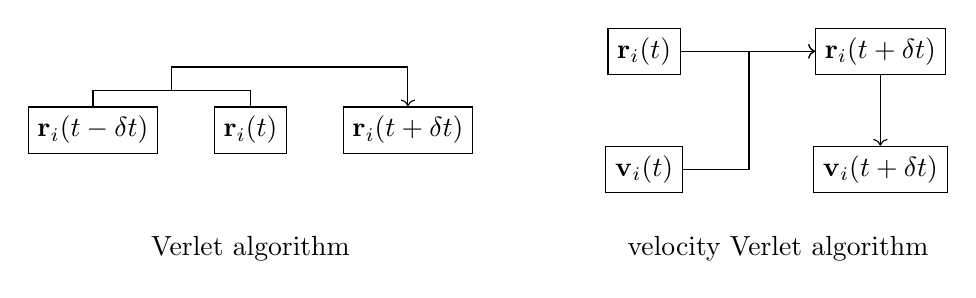
\begin{tikzpicture}
            \begin{scope}[shift={(-3.5,-1)}]
                \node[draw,fill=white] (E) at (0,0){\(\vb{r}_i(t-\delta t)\)};
                \node[draw,fill=white] (F) at (2,0){\(\vb{r}_i(t)\)};
                \node[draw,fill=white] (G) at (4,0){\(\vb{r}_i(t+\delta t)\)};
                \draw (E.north)--(0,0.5)--(2,0.5)--(F.north);
                \draw[->] (1,0.5)--(1,0.8)--(4,0.8)--(G.north);
                \node at (2,-1.5){Verlet algorithm};
            \end{scope}
            \begin{scope}[shift={(3.5,0)}]
                \node[draw] (A) at (0,0){\(\vb{r}_i(t)\)};
                \node[draw] (B) at (0,-1.5){\(\vb{v}_i(t)\)};
                \node[draw] (C) at (3,0){\(\vb{r}_i(t+\delta t)\)};
                \node[draw] (D) at (3,-1.5){\(\vb{v}_i(t+\delta t)\)};
                \draw[->] (A)--(C);
                \draw[fork] (B.east)--(C.west);
                \draw[->] (C)--(D);
                \node at (1.7,-2.5){velocity Verlet algorithm};
            \end{scope}
        \end{tikzpicture}
        \caption{Schemes of Verlet and velocity Verlet algorithms.}
    \end{figure}

    Now let's examine the accuracy of Verlet's algorithm using harmonic oscillator.

    \begin{figure}[ht!]
        \begin{subfigure}[h]{0.48\linewidth}
            \begin{adjustbox}{width=\linewidth}
            % This file was created with tikzplotlib v0.10.1.
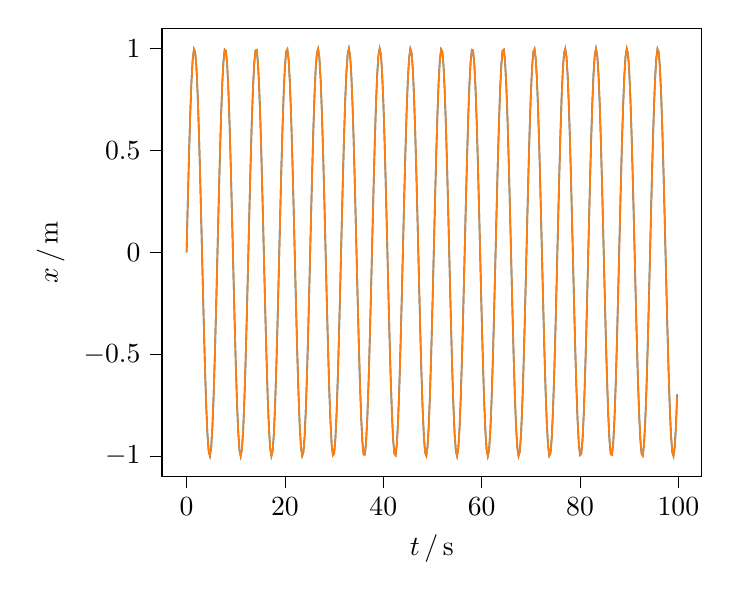
\begin{tikzpicture}

\definecolor{darkgray176}{RGB}{176,176,176}
\definecolor{darkorange25512714}{RGB}{255,127,14}
\definecolor{steelblue31119180}{RGB}{31,119,180}

\begin{axis}[
tick align=outside,
tick pos=left,
x grid style={darkgray176},
xlabel={\(\displaystyle t\,/\,\mathrm{s}\)},
xmin=-4.9875, xmax=104.7375,
xtick style={color=black},
y grid style={darkgray176},
ylabel={\(\displaystyle x\,/\,\mathrm{m}\)},
ymin=-1.10033, ymax=1.10033,
ytick style={color=black}
]
\addplot [semithick, steelblue31119180]
table {%
0 0
0.25 0.2475
0.5 0.4796
0.75 0.6819
1 0.8418
1.25 0.9493
1.5 0.9978
1.75 0.9843
2 0.9095
2.25 0.7782
2.5 0.5985
2.75 0.3815
3 0.1409
3.25 -0.1086
3.5 -0.3512
3.75 -0.5721
4 -0.7573
4.25 -0.8955
4.5 -0.9779
4.75 -0.9996
5 -0.9591
5.25 -0.8589
5.5 -0.7054
5.75 -0.5079
6 -0.2789
6.25 -0.0325
6.5 0.2158
6.75 0.4508
7 0.6577
7.25 0.8238
7.5 0.9386
7.75 0.995
8 0.9895
8.25 0.9226
8.5 0.7982
8.75 0.6242
9 0.4114
9.25 0.173
9.5 -0.0762
9.75 -0.3206
10 -0.5451
10.25 -0.7357
10.5 -0.8805
10.75 -0.9706
11 -1.0003
11.25 -0.9678
11.5 -0.8751
11.75 -0.7281
12 -0.5357
12.25 -0.31
12.5 -0.065
12.75 0.184
13 0.4215
13.25 0.6329
13.5 0.8049
13.75 0.9268
14 0.9911
14.25 0.9938
14.5 0.9346
14.75 0.8174
15 0.6493
15.25 0.4408
15.5 0.205
15.75 -0.0437
16 -0.2896
16.25 -0.5175
16.5 -0.7132
16.75 -0.8646
17 -0.9622
17.25 -0.9999
17.5 -0.9755
17.75 -0.8904
18 -0.75
18.25 -0.5629
18.5 -0.3408
18.75 -0.0975
19 0.1519
19.25 0.3918
19.5 0.6073
19.75 0.7851
20 0.9141
20.25 0.9862
20.5 0.997
20.75 0.9457
21 0.8357
21.25 0.6737
21.5 0.4698
21.75 0.2367
22 -0.0111
22.25 -0.2583
22.5 -0.4894
22.75 -0.69
23 -0.8478
23.25 -0.9528
23.5 -0.9985
23.75 -0.9822
24 -0.9048
24.25 -0.7711
24.5 -0.5895
24.75 -0.3712
25 -0.1298
25.25 0.1196
25.5 0.3616
25.75 0.5812
26 0.7645
26.25 0.9004
26.5 0.9802
26.75 0.9991
27 0.9558
27.25 0.8532
27.5 0.6974
27.75 0.4983
28 0.2682
28.25 0.0214
28.5 -0.2267
28.75 -0.4607
29 -0.6661
29.25 -0.83
29.5 -0.9424
29.75 -0.9961
30 -0.9879
30.25 -0.9182
30.5 -0.7914
30.75 -0.6155
31 -0.4012
31.25 -0.162
31.5 0.0873
31.75 0.3311
32 0.5544
32.25 0.7432
32.5 0.8857
32.75 0.9732
33 1.0002
33.25 0.9649
33.5 0.8697
33.75 0.7204
34 0.5262
34.25 0.2994
34.5 0.0539
34.75 -0.1949
35 -0.4316
35.25 -0.6415
35.5 -0.8114
35.75 -0.9309
36 -0.9926
36.25 -0.9925
36.5 -0.9306
36.75 -0.8109
37 -0.6408
37.25 -0.4308
37.5 -0.194
37.75 0.0548
38 0.3002
38.25 0.527
38.5 0.721
38.75 0.8701
39 0.9652
39.25 1.0002
39.5 0.973
39.75 0.8853
40 0.7426
40.25 0.5536
40.5 0.3303
40.75 0.0864
41 -0.1629
41.25 -0.402
41.5 -0.6162
41.75 -0.792
42 -0.9186
42.25 -0.988
42.5 -0.996
42.75 -0.9421
43 -0.8295
43.25 -0.6654
43.5 -0.4599
43.75 -0.2258
44 0.0223
44.25 0.269
44.5 0.4991
44.75 0.698
45 0.8536
45.25 0.9561
45.5 0.9991
45.75 0.98
46 0.9
46.25 0.764
46.5 0.5804
46.75 0.3608
47 0.1187
47.25 -0.1307
47.5 -0.372
47.75 -0.5902
48 -0.7717
48.25 -0.9052
48.5 -0.9824
48.75 -0.9985
49 -0.9525
49.25 -0.8473
49.5 -0.6894
49.75 -0.4886
50 -0.2574
50.25 -0.0102
50.5 0.2376
50.75 0.4706
51 0.6744
51.25 0.8362
51.5 0.946
51.75 0.997
52 0.986
52.25 0.9137
52.5 0.7846
52.75 0.6066
53 0.391
53.25 0.151
53.5 -0.0984
53.75 -0.3416
54 -0.5636
54.25 -0.7506
54.5 -0.8909
54.75 -0.9757
55 -0.9999
55.25 -0.9619
55.5 -0.8641
55.75 -0.7126
56 -0.5167
56.25 -0.2887
56.5 -0.0428
56.75 0.2058
57 0.4416
57.25 0.65
57.5 0.8179
57.75 0.935
58 0.9939
58.25 0.991
58.5 0.9265
58.75 0.8043
59 0.6322
59.25 0.4207
59.5 0.1831
59.75 -0.0659
60 -0.3109
60.25 -0.5364
60.5 -0.7287
60.75 -0.8756
61 -0.968
61.25 -1.0003
61.5 -0.9704
61.75 -0.8801
62 -0.735
62.25 -0.5443
62.5 -0.3197
62.75 -0.0753
63 0.1739
63.25 0.4122
63.5 0.6249
63.75 0.7987
64 0.9229
64.25 0.9897
64.5 0.9949
64.75 0.9383
65 0.8233
65.25 0.6571
65.5 0.45
65.75 0.215
66 -0.0334
66.25 -0.2798
66.5 -0.5087
66.75 -0.706
67 -0.8594
67.25 -0.9593
67.5 -0.9996
67.75 -0.9777
68 -0.8951
68.25 -0.7567
68.5 -0.5713
68.75 -0.3504
69 -0.1077
69.25 0.1417
69.5 0.3823
69.75 0.5992
70 0.7787
70.25 0.9099
70.5 0.9844
70.75 0.9978
71 0.949
71.25 0.8413
71.5 0.6813
71.75 0.4788
72 0.2466
72.25 -0.0009
72.5 -0.2484
72.75 -0.4804
73 -0.6826
73.25 -0.8423
73.5 -0.9496
73.75 -0.9979
74 -0.9841
74.25 -0.9091
74.5 -0.7776
74.75 -0.5977
75 -0.3807
75.25 -0.14
75.5 0.1095
75.75 0.3521
76 0.5728
76.25 0.7579
76.5 0.8959
76.75 0.9781
77 0.9996
77.25 0.9588
77.5 0.8585
77.75 0.7047
78 0.5071
78.25 0.278
78.5 0.0316
78.75 -0.2167
79 -0.4516
79.25 -0.6584
79.5 -0.8243
79.75 -0.9389
80 -0.9951
80.25 -0.9894
80.5 -0.9222
80.75 -0.7977
81 -0.6235
81.25 -0.4106
81.5 -0.1721
81.75 0.0771
82 0.3214
82.25 0.5458
82.5 0.7363
82.75 0.8809
83 0.9708
83.25 1.0003
83.5 0.9676
83.75 0.8747
84 0.7274
84.25 0.5349
84.5 0.3091
84.75 0.0641
85 -0.1848
85.25 -0.4223
85.5 -0.6336
85.75 -0.8054
86 -0.9271
86.25 -0.9912
86.5 -0.9937
86.75 -0.9343
87 -0.8169
87.25 -0.6486
87.5 -0.44
87.75 -0.2041
88 0.0446
88.25 0.2904
88.5 0.5183
88.75 0.7138
89 0.865
89.25 0.9624
89.5 1
89.75 0.9753
90 0.89
90.25 0.7494
90.5 0.5621
90.75 0.3399
91 0.0966
91.25 -0.1528
91.5 -0.3926
91.75 -0.6081
92 -0.7857
92.25 -0.9144
92.5 -0.9863
92.75 -0.9969
93 -0.9455
93.25 -0.8352
93.5 -0.673
93.75 -0.469
94 -0.2358
94.25 0.012
94.5 0.2592
94.75 0.4902
95 0.6907
95.25 0.8482
95.5 0.953
95.75 0.9986
96 0.982
96.25 0.9044
96.5 0.7705
96.75 0.5888
97 0.3704
97.25 0.1289
97.5 -0.1205
97.75 -0.3625
98 -0.5819
98.25 -0.7651
98.5 -0.9008
98.75 -0.9804
99 -0.9991
99.25 -0.9556
99.5 -0.8527
99.75 -0.6968
};
\addplot [semithick, darkorange25512714]
table {%
0 0
0.25 0.247
0.5 0.479
0.75 0.682
1 0.841
1.25 0.949
1.5 0.997
1.75 0.984
2 0.909
2.25 0.778
2.5 0.598
2.75 0.382
3 0.141
3.25 -0.108
3.5 -0.351
3.75 -0.572
4 -0.757
4.25 -0.895
4.5 -0.978
4.75 -0.999
5 -0.959
5.25 -0.859
5.5 -0.706
5.75 -0.508
6 -0.279
6.25 -0.033
6.5 0.215
6.75 0.45
7 0.657
7.25 0.823
7.5 0.938
7.75 0.995
8 0.989
8.25 0.923
8.5 0.798
8.75 0.625
9 0.412
9.25 0.174
9.5 -0.075
9.75 -0.32
10 -0.544
10.25 -0.735
10.5 -0.88
10.75 -0.97
11 -1
11.25 -0.968
11.5 -0.875
11.75 -0.729
12 -0.537
12.25 -0.311
12.5 -0.066
12.75 0.183
13 0.42
13.25 0.632
13.5 0.804
13.75 0.926
14 0.991
14.25 0.994
14.5 0.935
14.75 0.818
15 0.65
15.25 0.442
15.5 0.206
15.75 -0.042
16 -0.288
16.25 -0.516
16.5 -0.712
16.75 -0.863
17 -0.961
17.25 -1
17.5 -0.976
17.75 -0.891
18 -0.751
18.25 -0.564
18.5 -0.342
18.75 -0.099
19 0.15
19.25 0.39
19.5 0.606
19.75 0.784
20 0.913
20.25 0.986
20.5 0.997
20.75 0.946
21 0.837
21.25 0.675
21.5 0.472
21.75 0.239
22 -0.009
22.25 -0.256
22.5 -0.487
22.75 -0.688
23 -0.846
23.25 -0.952
23.5 -0.998
23.75 -0.982
24 -0.906
24.25 -0.772
24.5 -0.591
24.75 -0.373
25 -0.132
25.25 0.117
25.5 0.359
25.75 0.579
26 0.763
26.25 0.899
26.5 0.979
26.75 0.999
27 0.956
27.25 0.854
27.5 0.699
27.75 0.501
28 0.271
28.25 0.024
28.5 -0.224
28.75 -0.458
29 -0.664
29.25 -0.828
29.5 -0.941
29.75 -0.995
30 -0.988
30.25 -0.919
30.5 -0.793
30.75 -0.618
31 -0.404
31.25 -0.165
31.5 0.084
31.75 0.328
32 0.551
32.25 0.741
32.5 0.884
32.75 0.972
33 1
33.25 0.966
33.5 0.871
33.75 0.723
34 0.529
34.25 0.303
34.5 0.057
34.75 -0.191
35 -0.428
35.25 -0.638
35.5 -0.809
35.75 -0.929
36 -0.992
36.25 -0.993
36.5 -0.932
36.75 -0.813
37 -0.644
37.25 -0.434
37.5 -0.198
37.75 0.051
38 0.296
38.25 0.523
38.5 0.718
38.75 0.868
39 0.964
39.25 1
39.5 0.974
39.75 0.887
40 0.745
40.25 0.557
40.5 0.334
40.75 0.091
41 -0.159
41.25 -0.398
41.5 -0.613
41.75 -0.789
42 -0.917
42.25 -0.987
42.5 -0.996
42.75 -0.943
43 -0.832
43.25 -0.669
43.5 -0.464
43.75 -0.23
44 0.018
44.25 0.265
44.5 0.495
44.75 0.694
45 0.851
45.25 0.954
45.5 0.999
45.75 0.981
46 0.902
46.25 0.767
46.5 0.584
46.75 0.365
47 0.124
47.25 -0.126
47.5 -0.367
47.75 -0.586
48 -0.768
48.25 -0.903
48.5 -0.981
48.75 -0.998
49 -0.954
49.25 -0.85
49.5 -0.693
49.75 -0.493
50 -0.262
50.25 -0.015
50.5 0.232
50.75 0.466
51 0.67
51.25 0.833
51.5 0.944
51.75 0.996
52 0.987
52.25 0.916
52.5 0.788
52.75 0.611
53 0.396
53.25 0.156
53.5 -0.093
53.75 -0.336
54 -0.559
54.25 -0.747
54.5 -0.888
54.75 -0.974
55 -1
55.25 -0.963
55.5 -0.867
55.75 -0.716
56 -0.522
56.25 -0.294
56.5 -0.049
56.75 0.2
57 0.436
57.25 0.645
57.5 0.814
57.75 0.933
58 0.993
58.25 0.991
58.5 0.928
58.75 0.808
59 0.637
59.25 0.426
59.5 0.189
59.75 -0.06
60 -0.305
60.25 -0.531
60.5 -0.724
60.75 -0.872
61 -0.966
61.25 -1
61.5 -0.972
61.75 -0.883
62 -0.739
62.25 -0.55
62.5 -0.326
62.75 -0.082
63 0.167
63.25 0.406
63.5 0.62
63.75 0.794
64 0.92
64.25 0.988
64.5 0.995
64.75 0.94
65 0.827
65.25 0.662
65.5 0.456
65.75 0.222
66 -0.027
66.25 -0.273
66.5 -0.503
66.75 -0.701
67 -0.856
67.25 -0.957
67.5 -0.999
67.75 -0.979
68 -0.898
68.25 -0.761
68.5 -0.577
68.75 -0.357
69 -0.115
69.25 0.135
69.5 0.376
69.75 0.593
70 0.774
70.25 0.907
70.5 0.983
70.75 0.998
71 0.951
71.25 0.845
71.5 0.686
71.75 0.485
72 0.254
72.25 0.007
72.5 -0.241
72.75 -0.474
73 -0.677
73.25 -0.838
73.5 -0.947
73.75 -0.997
74 -0.985
74.25 -0.912
74.5 -0.782
74.75 -0.604
75 -0.388
75.25 -0.148
75.5 0.102
75.75 0.345
76 0.566
76.25 0.752
76.5 0.892
76.75 0.976
77 1
77.25 0.961
77.5 0.862
77.75 0.71
78 0.514
78.25 0.286
78.5 0.04
78.75 -0.209
79 -0.444
79.25 -0.652
79.5 -0.819
79.75 -0.936
80 -0.994
80.25 -0.99
80.5 -0.925
80.75 -0.802
81 -0.63
81.25 -0.418
81.5 -0.18
81.75 0.069
82 0.313
82.25 0.538
82.5 0.73
82.75 0.877
83 0.968
83.25 1
83.5 0.969
83.75 0.879
84 0.733
84.25 0.542
84.5 0.317
84.75 0.073
85 -0.176
85.25 -0.414
85.5 -0.626
85.75 -0.8
86 -0.923
86.25 -0.99
86.5 -0.994
86.75 -0.937
87 -0.822
87.25 -0.655
87.5 -0.448
87.75 -0.213
88 0.035
88.25 0.282
88.5 0.51
88.75 0.707
89 0.86
89.25 0.96
89.5 0.999
89.75 0.977
90 0.894
90.25 0.755
90.5 0.57
90.75 0.349
91 0.106
91.25 -0.143
91.5 -0.384
91.75 -0.6
92 -0.779
92.25 -0.91
92.5 -0.984
92.75 -0.997
93 -0.948
93.25 -0.84
93.5 -0.68
93.75 -0.477
94 -0.245
94.25 0.002
94.5 0.25
94.75 0.481
95 0.683
95.25 0.843
95.5 0.95
95.75 0.998
96 0.984
96.25 0.908
96.5 0.777
96.75 0.597
97 0.38
97.25 0.139
97.5 -0.11
97.75 -0.353
98 -0.573
98.25 -0.758
98.5 -0.896
98.75 -0.978
99 -0.999
99.25 -0.958
99.5 -0.858
99.75 -0.704
};
\end{axis}

\end{tikzpicture}

            \end{adjustbox}
            \caption{Displacement against time}
        \end{subfigure}
        \hfill
        \begin{subfigure}[h]{0.48\linewidth}
            \begin{adjustbox}{width=\linewidth}
            % This file was created with tikzplotlib v0.10.1.
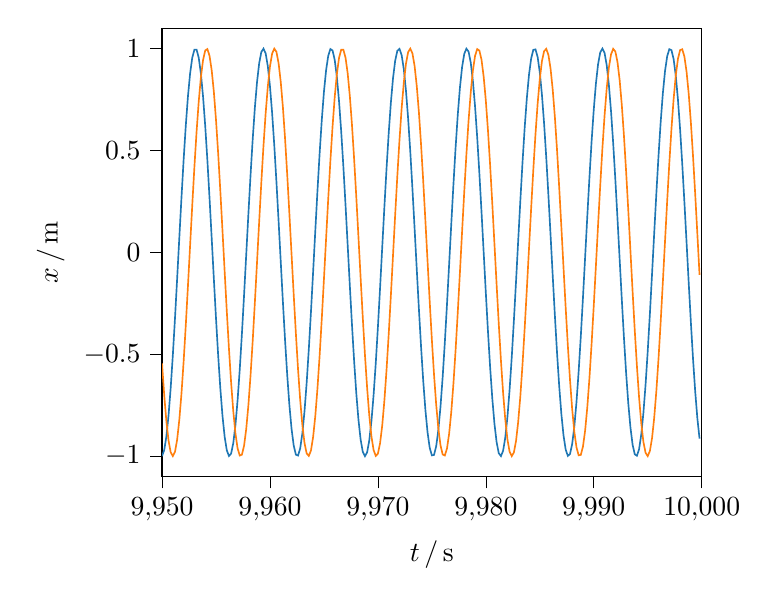
\begin{tikzpicture}

\definecolor{darkgray176}{RGB}{176,176,176}
\definecolor{darkorange25512714}{RGB}{255,127,14}
\definecolor{steelblue31119180}{RGB}{31,119,180}

\begin{axis}[
tick align=outside,
tick pos=left,
x grid style={darkgray176},
xlabel={\(\displaystyle t\,/\,\mathrm{s}\)},
xmin=9950, xmax=10000,
xtick style={color=black},
scaled ticks=false,
y grid style={darkgray176},
ylabel={\(\displaystyle x\,/\,\mathrm{m}\)},
ymin=-1.10033, ymax=1.10033,
ytick style={color=black}
]
\addplot [semithick, steelblue31119180]
table {%
9950 -0.9994
9950.2 -0.9712
9950.4 -0.9042
9950.6 -0.8011
9950.8 -0.6661
9951 -0.5045
9951.2 -0.3229
9951.4 -0.1283
9951.6 0.0714
9951.8 0.2682
9952 0.4543
9952.2 0.6223
9952.4 0.7655
9952.6 0.8782
9952.8 0.9558
9953 0.9954
9953.2 0.9952
9953.4 0.9554
9953.6 0.8775
9953.8 0.7646
9954 0.6211
9954.2 0.453
9954.4 0.2667
9954.6 0.0699
9954.8 -0.1298
9955 -0.3243
9955.2 -0.5058
9955.4 -0.6672
9955.6 -0.802
9955.8 -0.9048
9956 -0.9715
9956.2 -0.9995
9956.4 -0.9876
9956.6 -0.9364
9956.8 -0.8478
9957 -0.7254
9957.2 -0.574
9957.4 -0.3998
9957.6 -0.2097
9957.8 -0.0112
9958 0.1878
9958.2 0.3793
9958.4 0.5556
9958.6 0.7098
9958.8 0.8357
9959 0.9283
9959.2 0.9838
9959.4 1.0001
9959.6 0.9766
9959.8 0.9141
9960 0.8151
9960.2 0.6837
9960.4 0.525
9960.6 0.3453
9960.8 0.1519
9961 -0.0476
9961.2 -0.2452
9961.4 -0.433
9961.6 -0.6035
9961.8 -0.75
9962 -0.8665
9962.2 -0.9486
9962.4 -0.9927
9962.6 -0.9974
9962.8 -0.9622
9963 -0.8887
9963.2 -0.7797
9963.4 -0.6396
9963.6 -0.4741
9963.8 -0.2896
9964 -0.0936
9964.2 0.1062
9964.4 0.3017
9964.6 0.4852
9964.8 0.6493
9965 0.7875
9965.2 0.8944
9965.4 0.9656
9965.6 0.9982
9965.8 0.9911
9966 0.9445
9966.2 0.8602
9966.4 0.7415
9966.6 0.5934
9966.8 0.4215
9967 0.2329
9967.2 0.035
9967.4 -0.1644
9967.6 -0.3571
9967.8 -0.5357
9968 -0.6929
9968.2 -0.8224
9968.4 -0.9191
9968.6 -0.9792
9968.8 -1.0003
9969 -0.9815
9969.2 -0.9235
9969.4 -0.8287
9969.6 -0.7009
9969.8 -0.5451
9970 -0.3675
9970.2 -0.1754
9970.4 0.0238
9970.6 0.222
9970.8 0.4114
9971 0.5844
9971.2 0.734
9971.4 0.8544
9971.6 0.9407
9971.8 0.9895
9972 0.9989
9972.2 0.9684
9972.4 0.8993
9972.6 0.7944
9972.8 0.6577
9973 0.4949
9973.2 0.3123
9973.4 0.1173
9973.6 -0.0825
9973.8 -0.2789
9974 -0.4642
9974.2 -0.631
9974.4 -0.7726
9974.6 -0.8835
9974.8 -0.9591
9975 -0.9964
9975.2 -0.9941
9975.4 -0.952
9975.6 -0.8721
9975.8 -0.7573
9976 -0.6124
9976.2 -0.443
9976.4 -0.256
9976.6 -0.0587
9976.8 0.1408
9977 0.3348
9977.2 0.5154
9977.4 0.6755
9977.6 0.8086
9977.8 0.9095
9978 0.9741
9978.2 0.9999
9978.4 0.9858
9978.6 0.9324
9978.8 0.8418
9979 0.7176
9979.2 0.5649
9979.4 0.3896
9979.6 0.1988
9979.8 0
9980 -0.1987
9980.2 -0.3896
9980.4 -0.5649
9980.6 -0.7176
9980.8 -0.8418
9981 -0.9324
9981.2 -0.9858
9981.4 -0.9999
9981.6 -0.9741
9981.8 -0.9095
9982 -0.8086
9982.2 -0.6755
9982.4 -0.5154
9982.6 -0.3348
9982.8 -0.1409
9983 0.0587
9983.2 0.256
9983.4 0.443
9983.6 0.6124
9983.8 0.7573
9984 0.8721
9984.2 0.952
9984.4 0.9941
9984.6 0.9964
9984.8 0.9591
9985 0.8835
9985.2 0.7727
9985.4 0.631
9985.6 0.4642
9985.8 0.2789
9986 0.0825
9986.2 -0.1172
9986.4 -0.3123
9986.6 -0.4949
9986.8 -0.6577
9987 -0.7944
9987.2 -0.8993
9987.4 -0.9684
9987.6 -0.9989
9987.8 -0.9895
9988 -0.9407
9988.2 -0.8544
9988.4 -0.734
9988.6 -0.5844
9988.8 -0.4114
9989 -0.222
9989.2 -0.0238
9989.4 0.1754
9989.6 0.3675
9989.8 0.5451
9990 0.7008
9990.2 0.8287
9990.4 0.9235
9990.6 0.9815
9990.8 1.0003
9991 0.9792
9991.2 0.9191
9991.4 0.8224
9991.6 0.6929
9991.8 0.5357
9992 0.3572
9992.2 0.1644
9992.4 -0.0349
9992.6 -0.2329
9992.8 -0.4215
9993 -0.5934
9993.2 -0.7415
9993.4 -0.8602
9993.6 -0.9445
9993.8 -0.9911
9994 -0.9982
9994.2 -0.9656
9994.4 -0.8944
9994.6 -0.7876
9994.8 -0.6493
9995 -0.4852
9995.2 -0.3017
9995.4 -0.1062
9995.6 0.0936
9995.8 0.2896
9996 0.4741
9996.2 0.6396
9996.4 0.7797
9996.6 0.8886
9996.8 0.9622
9997 0.9974
9997.2 0.9927
9997.4 0.9486
9997.6 0.8666
9997.8 0.75
9998 0.6035
9998.2 0.433
9998.4 0.2452
9998.6 0.0476
9998.8 -0.1519
9999 -0.3453
9999.2 -0.5249
9999.4 -0.6837
9999.6 -0.8151
9999.8 -0.9141
};
\addplot [semithick, darkorange25512714]
table {%
9950 -0.545
9950.2 -0.7
9950.4 -0.828
9950.6 -0.923
9950.8 -0.981
9951 -1
9951.2 -0.979
9951.4 -0.919
9951.6 -0.822
9951.8 -0.693
9952 -0.536
9952.2 -0.357
9952.4 -0.165
9952.6 0.034
9952.8 0.232
9953 0.421
9953.2 0.593
9953.4 0.741
9953.6 0.86
9953.8 0.944
9954 0.991
9954.2 0.998
9954.4 0.965
9954.6 0.894
9954.8 0.788
9955 0.65
9955.2 0.486
9955.4 0.302
9955.6 0.107
9955.8 -0.093
9956 -0.289
9956.2 -0.473
9956.4 -0.639
9956.6 -0.779
9956.8 -0.888
9957 -0.962
9957.2 -0.997
9957.4 -0.993
9957.6 -0.949
9957.8 -0.867
9958 -0.75
9958.2 -0.604
9958.4 -0.434
9958.6 -0.246
9958.8 -0.049
9959 0.151
9959.2 0.344
9959.4 0.524
9959.6 0.683
9959.8 0.814
9960 0.913
9960.2 0.976
9960.4 1
9960.6 0.984
9960.8 0.928
9961 0.836
9961.2 0.711
9961.4 0.557
9961.6 0.38
9961.8 0.189
9962 -0.01
9962.2 -0.208
9962.4 -0.398
9962.6 -0.573
9962.8 -0.724
9963 -0.847
9963.2 -0.936
9963.4 -0.987
9963.6 -0.999
9963.8 -0.972
9964 -0.905
9964.2 -0.803
9964.4 -0.668
9964.6 -0.507
9964.8 -0.326
9965 -0.132
9965.2 0.068
9965.4 0.265
9965.6 0.451
9965.8 0.619
9966 0.763
9966.2 0.876
9966.4 0.955
9966.6 0.995
9966.8 0.995
9967 0.956
9967.2 0.879
9967.4 0.767
9967.6 0.624
9967.8 0.456
9968 0.27
9968.2 0.073
9968.4 -0.126
9968.6 -0.321
9968.8 -0.503
9969 -0.664
9969.2 -0.8
9969.4 -0.903
9969.6 -0.97
9969.8 -0.999
9970 -0.988
9970.2 -0.937
9970.4 -0.85
9970.6 -0.728
9970.8 -0.577
9971 -0.403
9971.2 -0.213
9971.4 -0.015
9971.6 0.184
9971.8 0.375
9972 0.552
9972.2 0.707
9972.4 0.833
9972.6 0.926
9972.8 0.983
9973 1
9973.2 0.977
9973.4 0.915
9973.6 0.817
9973.8 0.687
9974 0.528
9974.2 0.349
9974.4 0.156
9974.6 -0.043
9974.8 -0.241
9975 -0.429
9975.2 -0.6
9975.4 -0.747
9975.6 -0.864
9975.8 -0.947
9976 -0.992
9976.2 -0.997
9976.4 -0.963
9976.6 -0.89
9976.8 -0.782
9977 -0.643
9977.2 -0.478
9977.4 -0.294
9977.6 -0.098
9977.8 0.102
9978 0.297
9978.2 0.481
9978.4 0.646
9978.6 0.784
9978.8 0.892
9979 0.964
9979.2 0.998
9979.4 0.991
9979.6 0.946
9979.8 0.862
9980 0.745
9980.2 0.597
9980.4 0.426
9980.6 0.238
9980.8 0.04
9981 -0.159
9981.2 -0.352
9981.4 -0.531
9981.6 -0.689
9981.8 -0.819
9982 -0.917
9982.2 -0.978
9982.4 -1
9982.6 -0.982
9982.8 -0.925
9983 -0.831
9983.2 -0.704
9983.4 -0.549
9983.6 -0.372
9983.8 -0.18
9984 0.019
9984.2 0.217
9984.4 0.406
9984.6 0.58
9984.8 0.73
9985 0.851
9985.2 0.939
9985.4 0.988
9985.6 0.999
9985.8 0.969
9986 0.901
9986.2 0.797
9986.4 0.662
9986.6 0.5
9986.8 0.317
9987 0.123
9987.2 -0.077
9987.4 -0.273
9987.6 -0.459
9987.8 -0.626
9988 -0.769
9988.2 -0.881
9988.4 -0.957
9988.6 -0.996
9988.8 -0.994
9989 -0.953
9989.2 -0.875
9989.4 -0.761
9989.6 -0.617
9989.8 -0.448
9990 -0.262
9990.2 -0.065
9990.4 0.135
9990.6 0.329
9990.8 0.51
9991 0.671
9991.2 0.805
9991.4 0.907
9991.6 0.972
9991.8 0.999
9992 0.986
9992.2 0.934
9992.4 0.845
9992.6 0.722
9992.8 0.57
9993 0.395
9993.2 0.205
9993.4 0.006
9993.6 -0.193
9993.8 -0.384
9994 -0.559
9994.2 -0.713
9994.4 -0.838
9994.6 -0.93
9994.8 -0.984
9995 -1
9995.2 -0.975
9995.4 -0.912
9995.6 -0.812
9995.8 -0.68
9996 -0.521
9996.2 -0.341
9996.4 -0.147
9996.6 0.052
9996.8 0.25
9997 0.437
9997.2 0.607
9997.4 0.753
9997.6 0.869
9997.8 0.95
9998 0.993
9998.2 0.997
9998.4 0.961
9998.6 0.886
9998.8 0.777
9999 0.636
9999.2 0.47
9999.4 0.285
9999.6 0.089
9999.8 -0.11
};
\end{axis}

\end{tikzpicture}

            \end{adjustbox}
            \caption{Displacement at long \(t\)}
        \end{subfigure}\\
        \vskip 0.5cm
        \begin{subfigure}[h]{0.48\linewidth}
            \begin{adjustbox}{width=\linewidth}
            % This file was created with tikzplotlib v0.10.1.
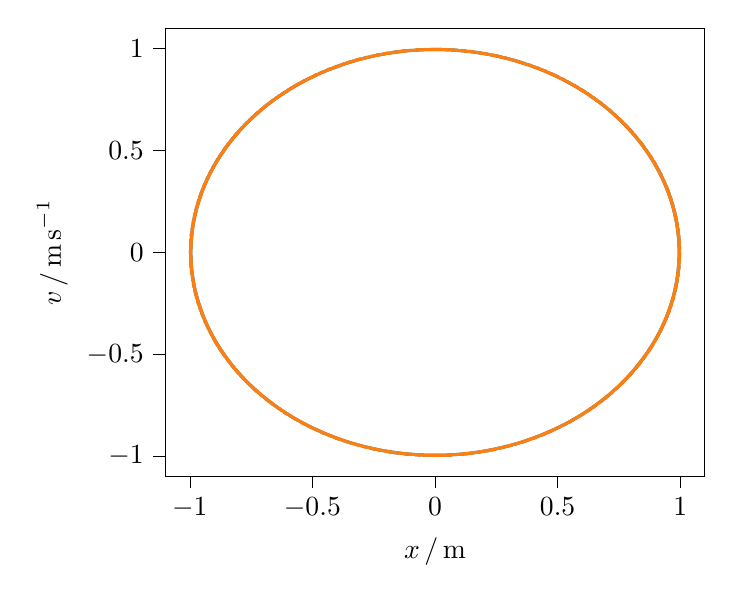
\begin{tikzpicture}

\definecolor{darkgray176}{RGB}{176,176,176}
\definecolor{darkorange25512714}{RGB}{255,127,14}
\definecolor{steelblue31119180}{RGB}{31,119,180}

\begin{axis}[
tick align=outside,
tick pos=left,
x grid style={darkgray176},
xlabel={\(\displaystyle x\,/\,\mathrm{m}\)},
xmin=-1.10033, xmax=1.10033,
xtick style={color=black},
y grid style={darkgray176},
ylabel={\(\displaystyle v\,/\,\mathrm{m\, s^{-1}}\)},
ymin=-1.1, ymax=1.1,
ytick style={color=black}
]
\addplot [semithick, steelblue31119180]
table {%
0 1
0.2475 0.969
0.4796 0.878
0.6819 0.732
0.8418 0.54
0.9493 0.315
0.9978 0.071
0.9843 -0.178
0.9095 -0.416
0.7782 -0.628
0.5985 -0.801
0.3815 -0.924
0.1409 -0.99
-0.1086 -0.994
-0.3512 -0.936
-0.5721 -0.82
-0.7573 -0.653
-0.8955 -0.446
-0.9779 -0.21
-0.9996 0.038
-0.9591 0.284
-0.8589 0.513
-0.7054 0.709
-0.5079 0.861
-0.2789 0.96
-0.0325 0.999
0.2158 0.976
0.4508 0.893
0.6577 0.753
0.8238 0.567
0.9386 0.346
0.995 0.103
0.9895 -0.146
0.9226 -0.387
0.7982 -0.603
0.6242 -0.781
0.4114 -0.912
0.173 -0.985
-0.0762 -0.997
-0.3206 -0.947
-0.5451 -0.839
-0.7357 -0.678
-0.8805 -0.475
-0.9706 -0.242
-1.0003 0.006
-0.9678 0.253
-0.8751 0.484
-0.7281 0.686
-0.5357 0.845
-0.31 0.951
-0.065 0.998
0.184 0.983
0.4215 0.907
0.6329 0.774
0.8049 0.594
0.9268 0.376
0.9911 0.135
0.9938 -0.114
0.9346 -0.356
0.8174 -0.576
0.6493 -0.761
0.4408 -0.898
0.205 -0.979
-0.0437 -0.999
-0.2896 -0.957
-0.5175 -0.856
-0.7132 -0.701
-0.8646 -0.503
-0.9622 -0.273
-0.9999 -0.027
-0.9755 0.221
-0.8904 0.456
-0.75 0.662
-0.5629 0.827
-0.3408 0.94
-0.0975 0.995
0.1519 0.988
0.3918 0.92
0.6073 0.795
0.7851 0.62
0.9141 0.406
0.9862 0.167
0.997 -0.082
0.9457 -0.326
0.8357 -0.55
0.6737 -0.739
0.4698 -0.883
0.2367 -0.972
-0.0111 -1
-0.2583 -0.966
-0.4894 -0.872
-0.69 -0.724
-0.8478 -0.531
-0.9528 -0.305
-0.9985 -0.059
-0.9822 0.189
-0.9048 0.426
-0.7711 0.637
-0.5895 0.808
-0.3712 0.929
-0.1298 0.992
0.1196 0.993
0.3616 0.932
0.5812 0.814
0.7645 0.645
0.9004 0.436
0.9802 0.199
0.9991 -0.049
0.9558 -0.295
0.8532 -0.522
0.6974 -0.717
0.4983 -0.867
0.2682 -0.963
0.0214 -1
-0.2267 -0.974
-0.4607 -0.888
-0.6661 -0.746
-0.83 -0.558
-0.9424 -0.335
-0.9961 -0.092
-0.9879 0.157
-0.9182 0.397
-0.7914 0.612
-0.6155 0.788
-0.4012 0.916
-0.162 0.987
0.0873 0.996
0.3311 0.944
0.5544 0.832
0.7432 0.669
0.8857 0.465
0.9732 0.231
1.0002 -0.017
0.9649 -0.264
0.8697 -0.494
0.7204 -0.694
0.5262 -0.85
0.2994 -0.954
0.0539 -0.999
-0.1949 -0.981
-0.4316 -0.902
-0.6415 -0.767
-0.8114 -0.585
-0.9309 -0.366
-0.9926 -0.124
-0.9925 0.125
-0.9306 0.367
-0.8109 0.586
-0.6408 0.768
-0.4308 0.903
-0.194 0.981
0.0548 0.998
0.3002 0.954
0.527 0.85
0.721 0.693
0.8701 0.493
0.9652 0.263
1.0002 0.016
0.973 -0.232
0.8853 -0.466
0.7426 -0.67
0.5536 -0.833
0.3303 -0.944
0.0864 -0.996
-0.1629 -0.987
-0.402 -0.916
-0.6162 -0.788
-0.792 -0.611
-0.9186 -0.396
-0.988 -0.156
-0.996 0.093
-0.9421 0.336
-0.8295 0.559
-0.6654 0.747
-0.4599 0.888
-0.2258 0.974
0.0223 1
0.269 0.963
0.4991 0.867
0.698 0.716
0.8536 0.521
0.9561 0.294
0.9991 0.048
0.98 -0.2
0.9 -0.436
0.764 -0.646
0.5804 -0.814
0.3608 -0.933
0.1187 -0.993
-0.1307 -0.991
-0.372 -0.928
-0.5902 -0.807
-0.7717 -0.636
-0.9052 -0.426
-0.9824 -0.188
-0.9985 0.06
-0.9525 0.305
-0.8473 0.532
-0.6894 0.725
-0.4886 0.873
-0.2574 0.966
-0.0102 1
0.2376 0.971
0.4706 0.882
0.6744 0.739
0.8362 0.549
0.946 0.325
0.997 0.081
0.986 -0.168
0.9137 -0.407
0.7846 -0.62
0.6066 -0.795
0.391 -0.92
0.151 -0.989
-0.0984 -0.995
-0.3416 -0.94
-0.5636 -0.826
-0.7506 -0.661
-0.8909 -0.455
-0.9757 -0.22
-0.9999 0.028
-0.9619 0.274
-0.8641 0.504
-0.7126 0.702
-0.5167 0.856
-0.2887 0.957
-0.0428 0.999
0.2058 0.979
0.4416 0.897
0.65 0.76
0.8179 0.576
0.935 0.355
0.9939 0.113
0.991 -0.136
0.9265 -0.377
0.8043 -0.595
0.6322 -0.775
0.4207 -0.907
0.1831 -0.983
-0.0659 -0.998
-0.3109 -0.95
-0.5364 -0.844
-0.7287 -0.685
-0.8756 -0.484
-0.968 -0.252
-1.0003 -0.005
-0.9704 0.243
-0.8801 0.475
-0.735 0.678
-0.5443 0.839
-0.3197 0.948
-0.0753 0.997
0.1739 0.985
0.4122 0.911
0.6249 0.781
0.7987 0.602
0.9229 0.386
0.9897 0.145
0.9949 -0.104
0.9383 -0.347
0.8233 -0.568
0.6571 -0.754
0.45 -0.893
0.215 -0.977
-0.0334 -0.999
-0.2798 -0.96
-0.5087 -0.861
-0.706 -0.708
-0.8594 -0.512
-0.9593 -0.283
-0.9996 -0.037
-0.9777 0.211
-0.8951 0.446
-0.7567 0.654
-0.5713 0.821
-0.3504 0.937
-0.1077 0.994
0.1417 0.99
0.3823 0.924
0.5992 0.801
0.7787 0.628
0.9099 0.416
0.9844 0.178
0.9978 -0.071
0.949 -0.316
0.8413 -0.541
0.6813 -0.732
0.4788 -0.878
0.2466 -0.969
-0.0009 -1
-0.2484 -0.969
-0.4804 -0.877
-0.6826 -0.731
-0.8423 -0.539
-0.9496 -0.314
-0.9979 -0.07
-0.9841 0.179
-0.9091 0.417
-0.7776 0.629
-0.5977 0.802
-0.3807 0.925
-0.14 0.99
0.1095 0.994
0.3521 0.936
0.5728 0.82
0.7579 0.653
0.8959 0.445
0.9781 0.209
0.9996 -0.039
0.9588 -0.285
0.8585 -0.513
0.7047 -0.71
0.5071 -0.862
0.278 -0.961
0.0316 -0.999
-0.2167 -0.976
-0.4516 -0.892
-0.6584 -0.753
-0.8243 -0.567
-0.9389 -0.345
-0.9951 -0.102
-0.9894 0.147
-0.9222 0.387
-0.7977 0.603
-0.6235 0.782
-0.4106 0.912
-0.1721 0.985
0.0771 0.997
0.3214 0.947
0.5458 0.838
0.7363 0.677
0.8809 0.474
0.9708 0.241
1.0003 -0.006
0.9676 -0.254
0.8747 -0.485
0.7274 -0.686
0.5349 -0.845
0.3091 -0.951
0.0641 -0.998
-0.1848 -0.983
-0.4223 -0.906
-0.6336 -0.774
-0.8054 -0.593
-0.9271 -0.375
-0.9912 -0.134
-0.9937 0.115
-0.9343 0.357
-0.8169 0.577
-0.6486 0.761
-0.44 0.898
-0.2041 0.979
0.0446 0.999
0.2904 0.957
0.5183 0.855
0.7138 0.701
0.865 0.502
0.9624 0.273
1 0.026
0.9753 -0.222
0.89 -0.456
0.7494 -0.662
0.5621 -0.827
0.3399 -0.94
0.0966 -0.995
-0.1528 -0.988
-0.3926 -0.92
-0.6081 -0.794
-0.7857 -0.619
-0.9144 -0.405
-0.9863 -0.167
-0.9969 0.083
-0.9455 0.327
-0.8352 0.55
-0.673 0.74
-0.469 0.883
-0.2358 0.972
0.012 1
0.2592 0.966
0.4902 0.872
0.6907 0.723
0.8482 0.53
0.953 0.304
0.9986 0.059
0.982 -0.19
0.9044 -0.427
0.7705 -0.638
0.5888 -0.808
0.3704 -0.929
0.1289 -0.992
-0.1205 -0.993
-0.3625 -0.932
-0.5819 -0.813
-0.7651 -0.644
-0.9008 -0.435
-0.9804 -0.199
-0.9991 0.05
-0.9556 0.296
-0.8527 0.523
-0.6968 0.718
};
\addplot [semithick, darkorange25512714]
table {%
0 1
0.2475 0.969
0.4796 0.878
0.6819 0.732
0.8418 0.54
0.9493 0.315
0.9978 0.071
0.9843 -0.178
0.9095 -0.416
0.7782 -0.628
0.5985 -0.801
0.3815 -0.924
0.1409 -0.99
-0.1086 -0.994
-0.3512 -0.936
-0.5721 -0.82
-0.7573 -0.653
-0.8955 -0.446
-0.9779 -0.21
-0.9996 0.038
-0.9591 0.284
-0.8589 0.513
-0.7054 0.709
-0.5079 0.861
-0.2789 0.96
-0.0325 0.999
0.2158 0.976
0.4508 0.893
0.6577 0.753
0.8238 0.567
0.9386 0.346
0.995 0.103
0.9895 -0.146
0.9226 -0.387
0.7982 -0.603
0.6242 -0.781
0.4114 -0.912
0.173 -0.985
-0.0762 -0.997
-0.3206 -0.947
-0.5451 -0.839
-0.7357 -0.678
-0.8805 -0.475
-0.9706 -0.242
-1.0003 0.006
-0.9678 0.253
-0.8751 0.484
-0.7281 0.686
-0.5357 0.845
-0.31 0.951
-0.065 0.998
0.184 0.983
0.4215 0.907
0.6329 0.774
0.8049 0.594
0.9268 0.376
0.9911 0.135
0.9938 -0.114
0.9346 -0.356
0.8174 -0.576
0.6493 -0.761
0.4408 -0.898
0.205 -0.979
-0.0437 -0.999
-0.2896 -0.957
-0.5175 -0.856
-0.7132 -0.701
-0.8646 -0.503
-0.9622 -0.273
-0.9999 -0.027
-0.9755 0.221
-0.8904 0.456
-0.75 0.662
-0.5629 0.827
-0.3408 0.94
-0.0975 0.995
0.1519 0.988
0.3918 0.92
0.6073 0.795
0.7851 0.62
0.9141 0.406
0.9862 0.167
0.997 -0.082
0.9457 -0.326
0.8357 -0.55
0.6737 -0.739
0.4698 -0.883
0.2367 -0.972
-0.0111 -1
-0.2583 -0.966
-0.4894 -0.872
-0.69 -0.724
-0.8478 -0.531
-0.9528 -0.305
-0.9985 -0.059
-0.9822 0.189
-0.9048 0.426
-0.7711 0.637
-0.5895 0.808
-0.3712 0.929
-0.1298 0.992
0.1196 0.993
0.3616 0.932
0.5812 0.814
0.7645 0.645
0.9004 0.436
0.9802 0.199
0.9991 -0.049
0.9558 -0.295
0.8532 -0.522
0.6974 -0.717
0.4983 -0.867
0.2682 -0.963
0.0214 -1
-0.2267 -0.974
-0.4607 -0.888
-0.6661 -0.746
-0.83 -0.558
-0.9424 -0.335
-0.9961 -0.092
-0.9879 0.157
-0.9182 0.397
-0.7914 0.612
-0.6155 0.788
-0.4012 0.916
-0.162 0.987
0.0873 0.996
0.3311 0.944
0.5544 0.832
0.7432 0.669
0.8857 0.465
0.9732 0.231
1.0002 -0.017
0.9649 -0.264
0.8697 -0.494
0.7204 -0.694
0.5262 -0.85
0.2994 -0.954
0.0539 -0.999
-0.1949 -0.981
-0.4316 -0.902
-0.6415 -0.767
-0.8114 -0.585
-0.9309 -0.366
-0.9926 -0.124
-0.9925 0.125
-0.9306 0.367
-0.8109 0.586
-0.6408 0.768
-0.4308 0.903
-0.194 0.981
0.0548 0.998
0.3002 0.954
0.527 0.85
0.721 0.693
0.8701 0.493
0.9652 0.263
1.0002 0.016
0.973 -0.232
0.8853 -0.466
0.7426 -0.67
0.5536 -0.833
0.3303 -0.944
0.0864 -0.996
-0.1629 -0.987
-0.402 -0.916
-0.6162 -0.788
-0.792 -0.611
-0.9186 -0.396
-0.988 -0.156
-0.996 0.093
-0.9421 0.336
-0.8295 0.559
-0.6654 0.747
-0.4599 0.888
-0.2258 0.974
0.0223 1
0.269 0.963
0.4991 0.867
0.698 0.716
0.8536 0.521
0.9561 0.294
0.9991 0.048
0.98 -0.2
0.9 -0.436
0.764 -0.646
0.5804 -0.814
0.3608 -0.933
0.1187 -0.993
-0.1307 -0.991
-0.372 -0.928
-0.5902 -0.807
-0.7717 -0.636
-0.9052 -0.426
-0.9824 -0.188
-0.9985 0.06
-0.9525 0.305
-0.8473 0.532
-0.6894 0.725
-0.4886 0.873
-0.2574 0.966
-0.0102 1
0.2376 0.971
0.4706 0.882
0.6744 0.739
0.8362 0.549
0.946 0.325
0.997 0.081
0.986 -0.168
0.9137 -0.407
0.7846 -0.62
0.6066 -0.795
0.391 -0.92
0.151 -0.989
-0.0984 -0.995
-0.3416 -0.94
-0.5636 -0.826
-0.7506 -0.661
-0.8909 -0.455
-0.9757 -0.22
-0.9999 0.028
-0.9619 0.274
-0.8641 0.504
-0.7126 0.702
-0.5167 0.856
-0.2887 0.957
-0.0428 0.999
0.2058 0.979
0.4416 0.897
0.65 0.76
0.8179 0.576
0.935 0.355
0.9939 0.113
0.991 -0.136
0.9265 -0.377
0.8043 -0.595
0.6322 -0.775
0.4207 -0.907
0.1831 -0.983
-0.0659 -0.998
-0.3109 -0.95
-0.5364 -0.844
-0.7287 -0.685
-0.8756 -0.484
-0.968 -0.252
-1.0003 -0.005
-0.9704 0.243
-0.8801 0.475
-0.735 0.678
-0.5443 0.839
-0.3197 0.948
-0.0753 0.997
0.1739 0.985
0.4122 0.911
0.6249 0.781
0.7987 0.602
0.9229 0.386
0.9897 0.145
0.9949 -0.104
0.9383 -0.347
0.8233 -0.568
0.6571 -0.754
0.45 -0.893
0.215 -0.977
-0.0334 -0.999
-0.2798 -0.96
-0.5087 -0.861
-0.706 -0.708
-0.8594 -0.512
-0.9593 -0.283
-0.9996 -0.037
-0.9777 0.211
-0.8951 0.446
-0.7567 0.654
-0.5713 0.821
-0.3504 0.937
-0.1077 0.994
0.1417 0.99
0.3823 0.924
0.5992 0.801
0.7787 0.628
0.9099 0.416
0.9844 0.178
0.9978 -0.071
0.949 -0.316
0.8413 -0.541
0.6813 -0.732
0.4788 -0.878
0.2466 -0.969
-0.0009 -1
-0.2484 -0.969
-0.4804 -0.877
-0.6826 -0.731
-0.8423 -0.539
-0.9496 -0.314
-0.9979 -0.07
-0.9841 0.179
-0.9091 0.417
-0.7776 0.629
-0.5977 0.802
-0.3807 0.925
-0.14 0.99
0.1095 0.994
0.3521 0.936
0.5728 0.82
0.7579 0.653
0.8959 0.445
0.9781 0.209
0.9996 -0.039
0.9588 -0.285
0.8585 -0.513
0.7047 -0.71
0.5071 -0.862
0.278 -0.961
0.0316 -0.999
-0.2167 -0.976
-0.4516 -0.892
-0.6584 -0.753
-0.8243 -0.567
-0.9389 -0.345
-0.9951 -0.102
-0.9894 0.147
-0.9222 0.387
-0.7977 0.603
-0.6235 0.782
-0.4106 0.912
-0.1721 0.985
0.0771 0.997
0.3214 0.947
0.5458 0.838
0.7363 0.677
0.8809 0.474
0.9708 0.241
1.0003 -0.006
0.9676 -0.254
0.8747 -0.485
0.7274 -0.686
0.5349 -0.845
0.3091 -0.951
0.0641 -0.998
-0.1848 -0.983
-0.4223 -0.906
-0.6336 -0.774
-0.8054 -0.593
-0.9271 -0.375
-0.9912 -0.134
-0.9937 0.115
-0.9343 0.357
-0.8169 0.577
-0.6486 0.761
-0.44 0.898
-0.2041 0.979
0.0446 0.999
0.2904 0.957
0.5183 0.855
0.7138 0.701
0.865 0.502
0.9624 0.273
1 0.026
0.9753 -0.222
0.89 -0.456
0.7494 -0.662
0.5621 -0.827
0.3399 -0.94
0.0966 -0.995
-0.1528 -0.988
-0.3926 -0.92
-0.6081 -0.794
-0.7857 -0.619
-0.9144 -0.405
-0.9863 -0.167
-0.9969 0.083
-0.9455 0.327
-0.8352 0.55
-0.673 0.74
-0.469 0.883
-0.2358 0.972
0.012 1
0.2592 0.966
0.4902 0.872
0.6907 0.723
0.8482 0.53
0.953 0.304
0.9986 0.059
0.982 -0.19
0.9044 -0.427
0.7705 -0.638
0.5888 -0.808
0.3704 -0.929
0.1289 -0.992
-0.1205 -0.993
-0.3625 -0.932
-0.5819 -0.813
-0.7651 -0.644
-0.9008 -0.435
-0.9804 -0.199
-0.9991 0.05
-0.9556 0.296
-0.8527 0.523
-0.6968 0.718
};
\end{axis}

\end{tikzpicture}

            \end{adjustbox}
            \caption{Phase diagram}
        \end{subfigure}
        \hfill
        \begin{subfigure}[h]{0.48\linewidth}
            \begin{adjustbox}{width=\linewidth}
            % This file was created with tikzplotlib v0.10.1.
\begin{tikzpicture}

\definecolor{darkgray176}{RGB}{176,176,176}
\definecolor{darkorange25512714}{RGB}{255,127,14}
\definecolor{steelblue31119180}{RGB}{31,119,180}

\begin{axis}[
tick align=outside,
tick pos=left,
x grid style={darkgray176},
xlabel={\(\displaystyle t\,/\,\mathrm{s}\)},
xmin=-497.5, xmax=10447.5,
xtick style={color=black},
scaled ticks=false,
y grid style={darkgray176},
ylabel={\(\displaystyle E\,/\,\mathrm{J}\)},
ymin=0, ymax=1,
ytick style={color=black}
]
\addplot [semithick, steelblue31119180]
table {%
0 0.5
50 0.5
100 0.5
150 0.5
200 0.5
250 0.5
300 0.5
350 0.5
400 0.5
450 0.5
500 0.5
550 0.5
600 0.5
650 0.5
700 0.5
750 0.5
800 0.5
850 0.5
900 0.5
950 0.5
1000 0.5
1050 0.5
1100 0.5
1150 0.5
1200 0.5
1250 0.5
1300 0.5
1350 0.5
1400 0.5
1450 0.5
1500 0.5
1550 0.5
1600 0.5
1650 0.5
1700 0.5
1750 0.5
1800 0.5
1850 0.5
1900 0.5
1950 0.5
2000 0.5
2050 0.5
2100 0.5
2150 0.5
2200 0.5
2250 0.5
2300 0.5
2350 0.5
2400 0.5
2450 0.5
2500 0.5
2550 0.5
2600 0.5
2650 0.5
2700 0.5
2750 0.5
2800 0.5
2850 0.5
2900 0.5
2950 0.5
3000 0.5
3050 0.5
3100 0.5
3150 0.5
3200 0.5
3250 0.5
3300 0.5
3350 0.5
3400 0.5
3450 0.5
3500 0.5
3550 0.5
3600 0.5
3650 0.5
3700 0.5
3750 0.5
3800 0.5
3850 0.5
3900 0.5
3950 0.5
4000 0.5
4050 0.5
4100 0.5
4150 0.5
4200 0.5
4250 0.5
4300 0.5
4350 0.5
4400 0.5
4450 0.5
4500 0.5
4550 0.5
4600 0.5
4650 0.5
4700 0.5
4750 0.5
4800 0.5
4850 0.5
4900 0.5
4950 0.5
5000 0.5
5050 0.5
5100 0.5
5150 0.5
5200 0.5
5250 0.5
5300 0.5
5350 0.5
5400 0.5
5450 0.5
5500 0.5
5550 0.5
5600 0.5
5650 0.5
5700 0.5
5750 0.5
5800 0.5
5850 0.5
5900 0.5
5950 0.5
6000 0.5
6050 0.5
6100 0.5
6150 0.5
6200 0.5
6250 0.5
6300 0.5
6350 0.5
6400 0.5
6450 0.5
6500 0.5
6550 0.5
6600 0.5
6650 0.5
6700 0.5
6750 0.5
6800 0.5
6850 0.5
6900 0.5
6950 0.5
7000 0.5
7050 0.5
7100 0.5
7150 0.5
7200 0.5
7250 0.5
7300 0.5
7350 0.5
7400 0.5
7450 0.5
7500 0.5
7550 0.5
7600 0.5
7650 0.5
7700 0.5
7750 0.5
7800 0.5
7850 0.5
7900 0.5
7950 0.5
8000 0.5
8050 0.5
8100 0.5
8150 0.5
8200 0.5
8250 0.5
8300 0.5
8350 0.5
8400 0.5
8450 0.5
8500 0.5
8550 0.5
8600 0.5
8650 0.5
8700 0.5
8750 0.5
8800 0.5
8850 0.5
8900 0.5
8950 0.5
9000 0.5
9050 0.5
9100 0.5
9150 0.5
9200 0.5
9250 0.5
9300 0.5
9350 0.5
9400 0.5
9450 0.5
9500 0.5
9550 0.5
9600 0.5
9650 0.5
9700 0.5
9750 0.5
9800 0.5
9850 0.5
9900 0.5
9950 0.5
};
\addplot [semithick, darkorange25512714]
table {%
0 0.5
50 0.5
100 0.5
150 0.5
200 0.5
250 0.5
300 0.5
350 0.5
400 0.5
450 0.5
500 0.5
550 0.5
600 0.5
650 0.5
700 0.5
750 0.5
800 0.5
850 0.5
900 0.5
950 0.5
1000 0.5
1050 0.5
1100 0.5
1150 0.5
1200 0.5
1250 0.5
1300 0.5
1350 0.5
1400 0.5
1450 0.5
1500 0.5
1550 0.5
1600 0.5
1650 0.5
1700 0.5
1750 0.5
1800 0.5
1850 0.5
1900 0.5
1950 0.5
2000 0.5
2050 0.5
2100 0.5
2150 0.5
2200 0.5
2250 0.5
2300 0.5
2350 0.5
2400 0.5
2450 0.5
2500 0.5
2550 0.5
2600 0.5
2650 0.5
2700 0.5
2750 0.5
2800 0.5
2850 0.5
2900 0.5
2950 0.5
3000 0.5
3050 0.5
3100 0.5
3150 0.5
3200 0.5
3250 0.5
3300 0.5
3350 0.5
3400 0.5
3450 0.5
3500 0.5
3550 0.5
3600 0.5
3650 0.5
3700 0.5
3750 0.5
3800 0.5
3850 0.5
3900 0.5
3950 0.5
4000 0.5
4050 0.5
4100 0.5
4150 0.5
4200 0.5
4250 0.5
4300 0.5
4350 0.5
4400 0.5
4450 0.5
4500 0.5
4550 0.5
4600 0.5
4650 0.5
4700 0.5
4750 0.5
4800 0.5
4850 0.5
4900 0.5
4950 0.5
5000 0.5
5050 0.5
5100 0.5
5150 0.5
5200 0.5
5250 0.5
5300 0.5
5350 0.5
5400 0.5
5450 0.5
5500 0.5
5550 0.5
5600 0.5
5650 0.5
5700 0.5
5750 0.5
5800 0.5
5850 0.5
5900 0.5
5950 0.5
6000 0.5
6050 0.5
6100 0.5
6150 0.5
6200 0.5
6250 0.5
6300 0.5
6350 0.5
6400 0.5
6450 0.5
6500 0.5
6550 0.5
6600 0.5
6650 0.5
6700 0.5
6750 0.5
6800 0.5
6850 0.5
6900 0.5
6950 0.5
7000 0.5
7050 0.5
7100 0.5
7150 0.5
7200 0.5
7250 0.5
7300 0.5
7350 0.5
7400 0.5
7450 0.5
7500 0.5
7550 0.5
7600 0.5
7650 0.5
7700 0.5
7750 0.5
7800 0.5
7850 0.5
7900 0.5
7950 0.5
8000 0.5
8050 0.5
8100 0.5
8150 0.5
8200 0.5
8250 0.5
8300 0.5
8350 0.5
8400 0.5
8450 0.5
8500 0.5
8550 0.5
8600 0.5
8650 0.5
8700 0.5
8750 0.5
8800 0.5
8850 0.5
8900 0.5
8950 0.5
9000 0.5
9050 0.5
9100 0.5
9150 0.5
9200 0.5
9250 0.5
9300 0.5
9350 0.5
9400 0.5
9450 0.5
9500 0.5
9550 0.5
9600 0.5
9650 0.5
9700 0.5
9750 0.5
9800 0.5
9850 0.5
9900 0.5
9950 0.5
};
\end{axis}

\end{tikzpicture}

            \end{adjustbox}
            \caption{Energy against time}
        \end{subfigure}%
        \caption{The motion of a harmonic oscillator solved by Verlet algorithm (blue) and the exact solution (orange). The step length in Verlet's method is also \(\delta t=0.05\unit{s}\).}
        \label{Fig:Verlet}
    \end{figure}

    We can see that the Verlet algorithm is very accurate. Although the displacements deviate from the exact displacement over time, the phase-space volume is conserved exactly and the total energy remains nearly constant (with only small bounded oscillations) over very long times.

    \subsubsection{Why use the Verlet Algorithm? (Non-examinable)}
    While there are algorithms with better short time accuracy than the Verlet algorithm, the overwhelming majority of condensed matter molecular dynamics simulations is based on just the Verlet algorithm. There are a number of reasons for its popularity.
    \begin{enumerate}[topsep=0pt,label=(\roman*)]
        \item The Verlet algorithm is simple and only depends on forces. No higher derivatives of the energy are needed. This is important because the force evaluation is the most CPU time consuming in MD simulations of interacting many-particle systems. Computation of higher derivatives of energy will increase computational costs substantially. Although the algorithms using force derivatives are more accurate, this gain is actually relatively minor. Because of the chaotic nature of the motion in many-particle systems, the particles rapidly deviate from the ``true'' trajectories. This is known as \textit{Lyapunov instability}: trajectories that differ slightly in initial conditions will diverge exponentially in time. If we denote \(\vb{r}(t)=\vb{r}(t\mid \vb{r}_0,\vb{p}_0)\) and \(\vb{r}'(t)=\vb{r}(t\mid \vb{r}_0,\vb{p}_0+\epsilon)\), then
        \begin{equation}
            \abs{\vb{r}(t)-\vb{r}'(t)}\sim\epsilon\exp(\lambda t)\,,
        \end{equation}
        where \(\lambda\) is the \textit{Lyapunov exponent}. This can be seen if we plot the logarithmic error of displacement against time, where the upper bound of the plot is a straight line with gradient \(\lambda\).

        \begin{figure}[ht!]
            \centering
            % This file was created with tikzplotlib v0.10.1.
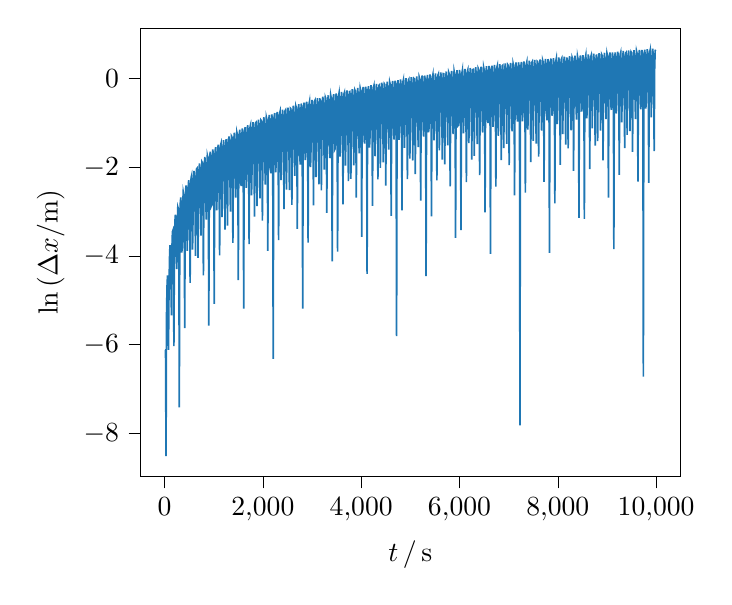
\begin{tikzpicture}

\definecolor{darkgray176}{RGB}{176,176,176}
\definecolor{steelblue31119180}{RGB}{31,119,180}

\begin{axis}[
tick align=outside,
tick pos=left,
unbounded coords=jump,
x grid style={darkgray176},
xlabel={\(\displaystyle t\,/\,\mathrm{s}\)},
xmin=-489, xmax=10489,
xtick style={color=black},
scaled ticks=false,
y grid style={darkgray176},
ylabel={\(\displaystyle \mathrm{ln}\,(\Delta x/\mathrm{m})\)},
ymin=-8.97685, ymax=1.13985,
ytick style={color=black}
]
\addplot [semithick, steelblue31119180]
table {%
0 -inf
10 -6.119
20 -6.119
30 -8.517
40 -5.339
50 -4.689
60 -4.44
70 -4.667
80 -6.119
90 -4.828
100 -4.075
110 -3.755
120 -3.922
130 -4.547
140 -5.339
150 -3.826
160 -3.455
170 -3.423
180 -3.772
190 -6.032
200 -3.932
210 -3.239
220 -3.07
230 -3.27
240 -4.063
250 -4.298
260 -3.239
270 -2.893
280 -2.93
290 -3.399
300 -7.419
310 -3.364
320 -2.81
330 -2.677
340 -2.919
350 -3.922
360 -3.808
370 -2.837
380 -2.551
390 -2.612
400 -3.156
410 -5.627
420 -2.984
430 -2.482
440 -2.406
450 -2.688
460 -3.882
470 -3.417
480 -2.526
490 -2.291
500 -2.401
510 -2.988
520 -4.605
530 -2.691
540 -2.233
550 -2.187
560 -2.533
570 -3.854
580 -3.058
590 -2.275
600 -2.083
610 -2.22
620 -2.904
630 -3.995
640 -2.435
650 -2.036
660 -2.022
670 -2.406
680 -4.04
690 -2.765
700 -2.079
710 -1.911
720 -2.094
730 -2.861
740 -3.54
750 -2.224
760 -1.873
770 -1.893
780 -2.323
790 -4.44
800 -2.521
810 -1.911
820 -1.767
830 -1.995
840 -2.847
850 -3.18
860 -2.034
870 -1.728
880 -1.78
890 -2.256
900 -5.573
910 -2.313
920 -1.749
930 -1.645
940 -1.905
950 -2.872
960 -2.844
970 -1.873
980 -1.597
990 -1.683
1000 -2.222
1010 -5.083
1020 -2.114
1030 -1.618
1040 -1.543
1050 -1.838
1060 -2.968
1070 -2.596
1080 -1.726
1090 -1.488
1100 -1.599
1110 -2.204
1120 -3.985
1130 -1.941
1140 -1.494
1150 -1.455
1160 -1.789
1170 -3.124
1180 -2.377
1190 -1.59
1200 -1.389
1210 -1.538
1220 -2.2
1230 -3.405
1240 -1.79
1250 -1.385
1260 -1.382
1270 -1.758
1280 -3.313
1290 -2.166
1300 -1.464
1310 -1.3
1320 -1.478
1330 -2.231
1340 -3
1350 -1.646
1360 -1.289
1370 -1.308
1380 -1.734
1390 -3.705
1400 -1.982
1410 -1.358
1420 -1.22
1430 -1.436
1440 -2.283
1450 -2.682
1460 -1.519
1470 -1.204
1480 -1.254
1490 -1.728
1500 -4.547
1510 -1.819
1520 -1.259
1530 -1.149
1540 -1.406
1550 -2.356
1560 -2.421
1570 -1.398
1580 -1.124
1590 -1.205
1600 -1.729
1610 -5.185
1620 -1.673
1630 -1.162
1640 -1.092
1650 -1.378
1660 -2.46
1670 -2.196
1680 -1.292
1690 -1.049
1700 -1.162
1710 -1.751
1720 -3.73
1730 -1.533
1740 -1.08
1750 -1.038
1760 -1.36
1770 -2.631
1780 -1.986
1790 -1.192
1800 -0.983
1810 -1.125
1820 -1.784
1830 -3.11
1840 -1.407
1850 -0.999
1860 -0.986
1870 -1.355
1880 -2.875
1890 -1.815
1900 -1.097
1910 -0.924
1920 -1.1
1930 -1.828
1940 -2.7
1950 -1.295
1960 -0.932
1970 -0.947
1980 -1.36
1990 -3.204
2000 -1.652
2010 -1.014
2020 -0.869
2030 -1.082
2040 -1.9
2050 -2.388
2060 -1.186
2070 -0.862
2080 -0.911
2090 -1.37
2100 -3.882
2110 -1.506
2120 -0.931
2130 -0.819
2140 -1.064
2150 -1.994
2160 -2.135
2170 -1.089
2180 -0.804
2190 -0.879
2200 -1.395
2210 -6.32
2220 -1.375
2230 -0.858
2240 -0.775
2250 -1.06
2260 -2.112
2270 -1.921
2280 -0.995
2290 -0.748
2300 -0.855
2310 -1.426
2320 -3.642
2330 -1.257
2340 -0.787
2350 -0.74
2360 -1.058
2370 -2.289
2380 -1.736
2390 -0.912
2400 -0.696
2410 -0.835
2420 -1.475
2430 -2.945
2440 -1.143
2450 -0.726
2460 -0.707
2470 -1.064
2480 -2.503
2490 -1.563
2500 -0.833
2510 -0.651
2520 -0.819
2530 -1.534
2540 -2.511
2550 -1.04
2560 -0.665
2570 -0.675
2580 -1.079
2590 -2.847
2600 -1.418
2610 -0.758
2620 -0.61
2630 -0.812
2640 -1.607
2650 -2.191
2660 -0.946
2670 -0.614
2680 -0.653
2690 -1.104
2700 -3.387
2710 -1.28
2720 -0.692
2730 -0.572
2740 -0.811
2750 -1.709
2760 -1.938
2770 -0.856
2780 -0.561
2790 -0.634
2800 -1.134
2810 -5.185
2820 -1.156
2830 -0.625
2840 -0.538
2850 -0.811
2860 -1.834
2870 -1.725
2880 -0.775
2890 -0.518
2900 -0.617
2910 -1.177
2920 -3.697
2930 -1.044
2940 -0.568
2950 -0.508
2960 -0.822
2970 -1.994
2980 -1.543
2990 -0.698
3000 -0.476
3010 -0.607
3020 -1.228
3030 -2.858
3040 -0.942
3050 -0.51
3060 -0.486
3070 -0.835
3080 -2.22
3090 -1.382
3100 -0.627
3110 -0.438
3120 -0.6
3130 -1.296
3140 -2.386
3150 -0.844
3160 -0.461
3170 -0.465
3180 -0.856
3190 -2.518
3200 -1.234
3210 -0.561
3220 -0.404
3230 -0.598
3240 -1.377
3250 -2.053
3260 -0.756
3270 -0.413
3280 -0.446
3290 -0.885
3300 -3.028
3310 -1.107
3320 -0.499
3330 -0.374
3340 -0.603
3350 -1.473
3360 -1.792
3370 -0.675
3380 -0.373
3390 -0.434
3400 -0.924
3410 -4.123
3420 -0.987
3430 -0.443
3440 -0.347
3450 -0.613
3460 -1.6
3470 -1.577
3480 -0.597
3490 -0.331
3500 -0.426
3510 -0.969
3520 -3.902
3530 -0.878
3540 -0.388
3550 -0.323
3560 -0.625
3570 -1.758
3580 -1.394
3590 -0.527
3600 -0.297
3610 -0.419
3620 -1.027
3630 -2.834
3640 -0.779
3650 -0.339
3660 -0.306
3670 -0.647
3680 -1.962
3690 -1.235
3700 -0.46
3710 -0.264
3720 -0.419
3730 -1.093
3740 -2.311
3750 -0.689
3760 -0.294
3770 -0.289
3780 -0.671
3790 -2.258
3800 -1.094
3810 -0.399
3820 -0.234
3830 -0.422
3840 -1.178
3850 -1.955
3860 -0.603
3870 -0.251
3880 -0.277
3890 -0.707
3900 -2.682
3910 -0.963
3920 -0.342
3930 -0.209
3940 -0.429
3950 -1.277
3960 -1.683
3970 -0.524
3980 -0.214
3990 -0.266
4000 -0.747
4010 -3.568
4020 -0.85
4030 -0.288
4040 -0.187
4050 -0.443
4060 -1.397
4070 -1.463
4080 -0.452
4090 -0.178
4100 -0.263
4110 -0.794
4120 -4.406
4130 -0.742
4140 -0.24
4150 -0.167
4160 -0.461
4170 -1.552
4180 -1.277
4190 -0.384
4200 -0.146
4210 -0.262
4220 -0.851
4230 -2.868
4240 -0.645
4250 -0.193
4260 -0.151
4270 -0.483
4280 -1.749
4290 -1.117
4300 -0.321
4310 -0.117
4320 -0.263
4330 -0.921
4340 -2.271
4350 -0.557
4360 -0.152
4370 -0.14
4380 -0.513
4390 -2.01
4400 -0.976
4410 -0.262
4420 -0.091
4430 -0.27
4440 -1.003
4450 -1.888
4460 -0.475
4470 -0.113
4480 -0.131
4490 -0.546
4500 -2.41
4510 -0.85
4520 -0.209
4530 -0.068
4540 -0.281
4550 -1.104
4560 -1.601
4570 -0.398
4580 -0.077
4590 -0.125
4600 -0.591
4610 -3.092
4620 -0.732
4630 -0.159
4640 -0.049
4650 -0.298
4660 -1.223
4670 -1.374
4680 -0.328
4690 -0.045
4700 -0.121
4710 -0.642
4720 -5.809
4730 -0.63
4740 -0.111
4750 -0.033
4760 -0.316
4770 -1.377
4780 -1.184
4790 -0.263
4800 -0.016
4810 -0.124
4820 -0.699
4830 -2.968
4840 -0.533
4850 -0.069
4860 -0.019
4870 -0.342
4880 -1.558
4890 -1.021
4900 -0.202
4910 0.01
4920 -0.129
4930 -0.767
4940 -2.265
4950 -0.446
4960 -0.028
4970 -0.009
4980 -0.371
4990 -1.804
5000 -0.878
5010 -0.146
5020 0.034
5030 -0.137
5040 -0.851
5050 -1.845
5060 -0.365
5070 0.007
5080 -0.004
5090 -0.409
5100 -2.151
5110 -0.751
5120 -0.093
5130 0.054
5140 -0.15
5150 -0.947
5160 -1.543
5170 -0.292
5180 0.04
5190 0
5200 -0.451
5210 -2.749
5220 -0.638
5230 -0.046
5240 0.072
5250 -0.167
5260 -1.067
5270 -1.305
5280 -0.222
5290 0.071
5300 0
5310 -0.505
5320 -4.457
5330 -0.531
5340 -0.001
5350 0.085
5360 -0.19
5370 -1.209
5380 -1.109
5390 -0.158
5400 0.097
5410 -0.003
5420 -0.564
5430 -3.106
5440 -0.439
5450 0.041
5460 0.097
5470 -0.215
5480 -1.391
5490 -0.942
5500 -0.099
5510 0.122
5520 -0.009
5530 -0.632
5540 -2.293
5550 -0.351
5560 0.078
5570 0.105
5580 -0.248
5590 -1.616
5600 -0.797
5610 -0.044
5620 0.143
5630 -0.02
5640 -0.712
5650 -1.825
5660 -0.27
5670 0.114
5680 0.111
5690 -0.284
5700 -1.935
5710 -0.668
5720 0.006
5730 0.162
5740 -0.033
5750 -0.809
5760 -1.501
5770 -0.197
5780 0.144
5790 0.111
5800 -0.329
5810 -2.43
5820 -0.554
5830 0.054
5840 0.178
5850 -0.052
5860 -0.922
5870 -1.252
5880 -0.13
5890 0.173
5900 0.11
5910 -0.379
5920 -3.59
5930 -0.45
5940 0.096
5950 0.191
5960 -0.074
5970 -1.061
5980 -1.049
5990 -0.066
6000 0.199
6010 0.106
6020 -0.441
6030 -3.417
6040 -0.354
6050 0.136
6060 0.2
6070 -0.103
6080 -1.231
6090 -0.877
6100 -0.008
6110 0.221
6120 0.097
6130 -0.51
6140 -2.333
6150 -0.269
6160 0.173
6170 0.207
6180 -0.134
6190 -1.452
6200 -0.729
6210 0.045
6220 0.241
6230 0.087
6240 -0.588
6250 -1.828
6260 -0.189
6270 0.206
6280 0.211
6290 -0.173
6300 -1.738
6310 -0.598
6320 0.095
6330 0.258
6340 0.071
6350 -0.681
6360 -1.477
6370 -0.115
6380 0.237
6390 0.211
6400 -0.216
6410 -2.177
6420 -0.482
6430 0.141
6440 0.273
6450 0.053
6460 -0.793
6470 -1.213
6480 -0.048
6490 0.264
6500 0.209
6510 -0.268
6520 -3.016
6530 -0.378
6540 0.182
6550 0.285
6560 0.029
6570 -0.924
6580 -1.001
6590 0.014
6600 0.288
6610 0.204
6620 -0.326
6630 -3.953
6640 -0.283
6650 0.222
6660 0.294
6670 0.001
6680 -1.088
6690 -0.824
6700 0.072
6710 0.311
6720 0.195
6730 -0.396
6740 -2.437
6750 -0.195
6760 0.258
6770 0.299
6780 -0.033
6790 -1.292
6800 -0.672
6810 0.125
6820 0.329
6830 0.182
6840 -0.475
6850 -1.838
6860 -0.117
6870 0.291
6880 0.302
6890 -0.07
6900 -1.568
6910 -0.539
6920 0.174
6930 0.346
6940 0.167
6950 -0.565
6960 -1.468
6970 -0.043
6980 0.319
6990 0.302
7000 -0.115
7010 -1.952
7020 -0.421
7030 0.219
7040 0.359
7050 0.147
7060 -0.676
7070 -1.187
7080 0.024
7090 0.347
7100 0.298
7110 -0.167
7120 -2.634
7130 -0.315
7140 0.261
7150 0.37
7160 0.124
7170 -0.801
7180 -0.965
7190 0.086
7200 0.37
7210 0.293
7220 -0.224
7230 -7.824
7240 -0.219
7250 0.298
7260 0.378
7270 0.095
7280 -0.96
7290 -0.781
7300 0.143
7310 0.391
7320 0.283
7330 -0.293
7340 -2.572
7350 -0.133
7360 0.334
7370 0.382
7380 0.062
7390 -1.15
7400 -0.624
7410 0.196
7420 0.41
7430 0.27
7440 -0.37
7450 -1.883
7460 -0.052
7470 0.366
7480 0.386
7490 0.023
7500 -1.401
7510 -0.488
7520 0.243
7530 0.425
7540 0.254
7550 -0.459
7560 -1.464
7570 0.02
7580 0.395
7590 0.385
7600 -0.02
7610 -1.76
7620 -0.368
7630 0.289
7640 0.438
7650 0.234
7660 -0.562
7670 -1.172
7680 0.088
7690 0.421
7700 0.381
7710 -0.071
7720 -2.325
7730 -0.26
7740 0.33
7750 0.448
7760 0.21
7770 -0.689
7780 -0.939
7790 0.15
7800 0.443
7810 0.374
7820 -0.13
7830 -3.932
7840 -0.164
7850 0.369
7860 0.455
7870 0.182
7880 -0.834
7890 -0.747
7900 0.208
7910 0.465
7920 0.364
7930 -0.195
7940 -2.81
7950 -0.076
7960 0.402
7970 0.46
7980 0.149
7990 -1.022
8000 -0.586
8010 0.26
8020 0.482
8030 0.351
8040 -0.272
8050 -1.941
8060 0.004
8070 0.435
8080 0.461
8090 0.111
8100 -1.252
8110 -0.446
8120 0.309
8130 0.498
8140 0.334
8150 -0.359
8160 -1.485
8170 0.079
8180 0.463
8190 0.461
8200 0.066
8210 -1.573
8220 -0.323
8230 0.352
8240 0.509
8250 0.314
8260 -0.461
8270 -1.163
8280 0.145
8290 0.488
8300 0.457
8310 0.017
8320 -2.078
8330 -0.213
8340 0.394
8350 0.519
8360 0.29
8370 -0.578
8380 -0.922
8390 0.208
8400 0.511
8410 0.45
8420 -0.04
8430 -3.142
8440 -0.115
8450 0.431
8460 0.526
8470 0.262
8480 -0.724
8490 -0.722
8500 0.265
8510 0.531
8520 0.439
8530 -0.106
8540 -3.161
8550 -0.026
8560 0.466
8570 0.531
8580 0.229
8590 -0.895
8600 -0.554
8610 0.318
8620 0.549
8630 0.426
8640 -0.179
8650 -2.042
8660 0.055
8670 0.497
8680 0.532
8690 0.191
8700 -1.12
8710 -0.41
8720 0.366
8730 0.563
8740 0.409
8750 -0.266
8760 -1.512
8770 0.129
8780 0.526
8790 0.53
8800 0.148
8810 -1.41
8820 -0.284
8830 0.411
8840 0.576
8850 0.389
8860 -0.364
8870 -1.171
8880 0.198
8890 0.551
8900 0.526
8910 0.098
8920 -1.845
8930 -0.172
8940 0.451
8950 0.585
8960 0.364
8970 -0.48
8980 -0.909
8990 0.259
9000 0.573
9010 0.519
9020 0.043
9030 -2.685
9040 -0.072
9050 0.489
9060 0.591
9070 0.336
9080 -0.614
9090 -0.704
9100 0.317
9110 0.593
9120 0.508
9130 -0.021
9140 -3.844
9150 0.018
9160 0.523
9170 0.595
9180 0.304
9190 -0.784
9200 -0.53
9210 0.37
9220 0.61
9230 0.495
9240 -0.095
9250 -2.168
9260 0.1
9270 0.555
9280 0.597
9290 0.265
9300 -0.987
9310 -0.381
9320 0.419
9330 0.625
9340 0.478
9350 -0.177
9360 -1.566
9370 0.175
9380 0.582
9390 0.595
9400 0.224
9410 -1.264
9420 -0.252
9430 0.463
9440 0.636
9450 0.458
9460 -0.274
9470 -1.184
9480 0.243
9490 0.608
9500 0.59
9510 0.174
9520 -1.649
9530 -0.137
9540 0.503
9550 0.645
9560 0.434
9570 -0.385
9580 -0.91
9590 0.307
9600 0.63
9610 0.584
9620 0.12
9630 -2.319
9640 -0.035
9650 0.541
9660 0.652
9670 0.405
9680 -0.517
9690 -0.69
9700 0.364
9710 0.649
9720 0.573
9730 0.058
9740 -6.725
9750 0.057
9760 0.576
9770 0.656
9780 0.373
9790 -0.673
9800 -0.512
9810 0.418
9820 0.666
9830 0.559
9840 -0.014
9850 -2.348
9860 0.14
9870 0.606
9880 0.656
9890 0.336
9900 -0.872
9910 -0.358
9920 0.466
9930 0.68
9940 0.542
9950 -0.096
9960 -1.631
9970 0.216
9980 0.635
9990 0.655
};
\end{axis}

\end{tikzpicture}

            \caption{Logarithmic error of displacement of a harmonic oscillator using Verlet algorithm.}
        \end{figure}
        
        Having an exponentially growing error may seems horrible, but it is actually not as big a problem as it seems!
        \begin{thm}[Shadowing theorem]
            Every numerical trajectory will be uniformly close to some true trajectory with slightly altered initial position. In other words, a numerical trajectory is ``shadowed'' by a true one.
        \end{thm}
        \begin{figure}[ht!]
            \centering
            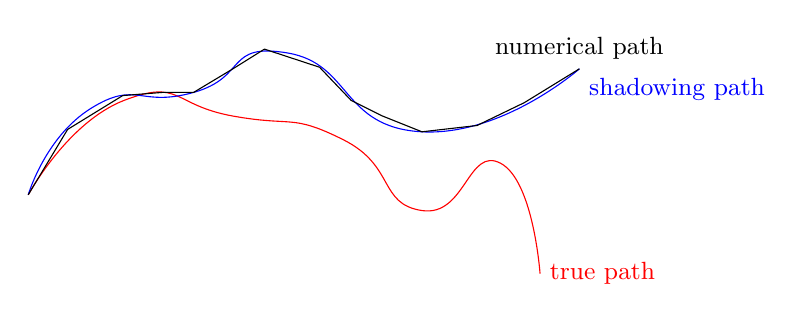
\begin{tikzpicture}
                \draw[red] plot[smooth, tension = 1] coordinates {(0,0) (1.22,1.2) (2.6,1) (4,0.7) (5,-0.2) (6,0.4) (6.5,-1) };
                \node[red] at (6.5,-1) [right]{\small true path};
                \draw[blue] plot[smooth, tension = 1] coordinates {(0,0) (0.8,1.1) (2.1,1.3) (3.3,1.8) (5,0.8) (7,1.6) };
                \draw (0,0) -- (0.5,0.83) -- (1.2,1.26) -- (1.7,1.3) -- (2.1,1.3) -- (2.6,1.6) -- (3,1.85) -- (3.7,1.62) -- (4.1,1.2) -- (4.5,1) -- (5,0.8) --(5.7,0.88) -- (6.3,1.17) -- (7,1.6);
                \node[blue] at (7,1.6) [below right]{\small shadowing path};
                \node at (7,1.6) [above]{\small numerical path};
            \end{tikzpicture}
        \end{figure}

        This strong molecular chaos is ultimately the justification of methods of statistical mechanics.
        \item Even though it only uses forces, the Verlet algorithm is correct up to and including \(O(\delta t^3)\).
        \item The Verlet algorithm is explicitly time reversible and, even though the trajectory relatively quickly diverges substantially from the true trajectory, the energy is conserved over an extremely long period of time. Moreover, the Verlet algorithm rigorously conserves the normalisation of an ensemble probability distribution of points in phase space. In more advanced language, the Verlet integrator is said to be \textit{symplectic}. These formal properties contribute to the superior long time stability of the Verlet algorithm.
        
        For example, as we will discuss later, energy is the defining quantity for the microcanonical ensemble, since, for chaotic systems, there are no constraints on the regions trajectories can reach in phase space other than that they are confined to the hypersurface of constant energy. Energy conservation, together with norm conservation are therefore necessary conditions for thermodynamic stability, and ultimately for a proper definition of temperature. Long time stability is particularly important for the simulation of liquids which are stabilised by finite temperature dynamical fluctuations.
    \end{enumerate}

    \subsection{Connection to Equilibrium Statistical Mechanics}
    \subsubsection{The Microcanonical Ensemble}
    So far, we have studied systems using Newtonian dynamics, in which the energy is naturally conserved if the system is closed. This corresponds to a microcanonical ensemble. For each observable \(A\) of the system, there is a corresponding \textit{phase function} \(\mathcal{A}(\vb{r}^N,\vb{p}^N)\) telling us the value of \(A\) given a state \((\vb{r}^N,\vb{p}^N)\) of the system. Then the ensemble average of the system is given by
    \begin{equation}\label{microcanonical_average}
        \eval{A}_{NVE}=\int\dd[3N]{\vb{r}^N}\dd[3N]{\vb{p}^N}\rho_{NVE}(\vb{r}^N,\vb{p}^N)\mathcal{A}(\vb{r}^N,\vb{p}^{N})\,,
    \end{equation}
    where \(\rho_{NVE}(\vb{r}^N,\vb{p}^N)\) is the \textit{microcanonical phase-space distribution function} restricting the manifold of accessible phase points \((\vb{r}^N,\vb{p}^N)\) to a hypersurface of constant energy \(E\) only, given by
    \begin{equation}
        \rho_{NVE}(\vb{r}^N,\vb{p}^N)=\frac{f(N)}{\Omega_N}\delta(\mathcal{H}(\vb{r}^N,\vb{p}^N)-E)\,.
    \end{equation}
    The phase function \(\mathcal{H}(\vb{r}^N,\vb{p}^N)\) is the Hamiltonian, \(f(N)\) is some function of the number of particles accounting for their indistinguishability, and \(\Omega_N\) is the microcanonical partition function given by
    \begin{equation}
        \Omega_N=f(N)\int\dd[3N]{\vb{r}^N}\dd[3N]{\vb{p}^N}\delta(\mathcal{H}(\vb{r}^N,\vb{p}^N)-E)\,.
    \end{equation}
    The factors \(f(N)\) in the above expression can be omitted if we are only interested in mechanical observable averages over the ensemble distributions using \(\rho_{NVE}\), but it becomes crucial if we want to give the normalisation factor \(\Omega_N\) a thermodynamical interpretation when calculating entropy, free energy \textit{etc.}

    \subsubsection{The Ergodic Principle and Time Averages}
    The above thermodynamic average of a quantity require us to evaluate it over the whole hypersurface of constant energy \(\mathcal{H}(\vb{r}^N,\vb{p}^N)\) in the phase space --- it is difficult to do this in a computer simulation. However, we know that the state of a deterministic \(NVE\) system also evolves on this hypersurface of constant energy with time, with trajectory \((\vb{r}^N(t),\vb{p}^N(t))\). This allows us to determine how the physical observable \(A\) evolve along a certain trajectory as a function of time
    \begin{equation}
        A(t)\equiv \mathcal{A}(\vb{r}^N(t),\vb{p}^N(t))\,.
    \end{equation}
    Now we are going to invoke some hypothesis.
    \begin{hyp}[Ergodic Hypothesis]
        Over a long enough period of time, the time spent by a system in some region of the phase space of microstates with the same energy is proportional to the volume of this region, i.e., that all accessible microstates are equiprobable over a long period of time.
    \end{hyp}
    This means that if we let our system evolves for a long period of time, then it will go over the whole subset of the phase space that it is allowed to go to --- it is not saying that it will travel to every single point in the hypersurface of constant energy, which is impossible for a finite amount of time. What we are saying is that the system is sampling through a large enough portion of the phase space, so that the time average of the quantity \(A(t)\) is essentially the ensemble average \(\eval{A}_{NVE}\). We are replacing the ensemble average with a time average from a very long trajectory.
    \begin{equation}
        \eval{A}_{NVE}=\lim_{\tau\to\infty}\overline{A}_{\tau}=\lim_{\tau\to\infty}\frac{1}{\tau}\int_{0}^{\tau}\dd{t}\mathcal{A}(\vb{r}^N(t),\vb{p}^N(t))\,.
    \end{equation}
    In molecular dynamics computer simulation, we can only approximate a discrete path of time interval \(\delta t\) over a finite amount of time \(\tau=M\delta t\). We then need to replace the above integral by a sum.
    \begin{equation}
        \eval{A}_{\tau}\approx\frac{1}{M}\sum_{m=1}^{M}\mathcal{A}(\vb{r}^N(t_m),\vb{p}^N(t_m))\,.
    \end{equation}
    
    \begin{figure}[ht!]
        \centering
        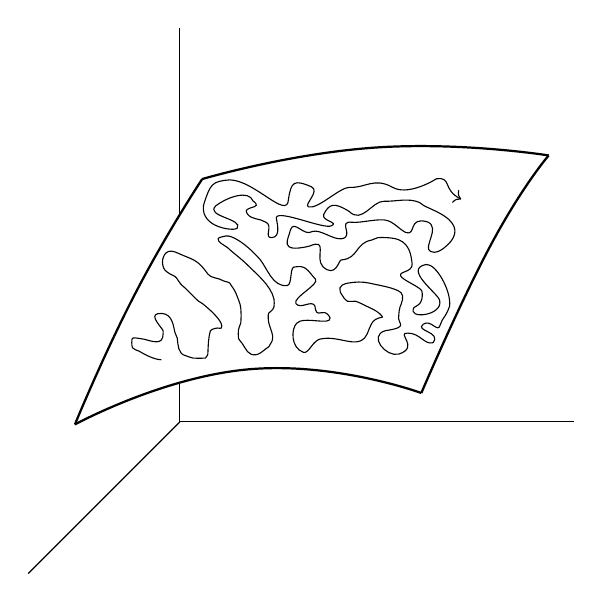
\begin{tikzpicture}
            \draw (0,0)--(5,0);
            \draw (0,0)--(0,0.5);
            \draw (0,2.63)--(0,5);
            \draw (0,0)--(0,0,5);
            \draw[thick] plot[smooth, tension = 0.9] coordinates {(0.4,1.7,4.5) (0.4,2.6,2.5) (0.4,3.2,0.3)};
            \draw[thick] plot[smooth, tension = 0.9] coordinates {(0.4,1.7,4.5) (2.6,2.4,4.5) (4.8,2.1,4.5)};
            \draw[thick] plot[smooth, tension = 0.9] coordinates {(0.4,3.2,0.3) (2.6,3.6,0.3) (4.8,3.5,0.3)};
            \draw[thick] plot[smooth, tension = 0.9] coordinates {(4.8,2.1,4.5) (4.8,3.1,2.2) (4.8,3.5,0.3)};
            \begin{scope}[shift={(-2.1,0.1)}]
                \draw [scale=0.23,->] (8.11,3) .. controls (7.73,3) and (7.19,3.29) .. (6.89,3.47) .. controls (6.79,3.54) and (6.58,3.54) .. (6.52,3.66) .. controls (6.46,3.77) and (6.48,4.09) .. (6.49,4.13) .. controls (6.5,4.28) and (6.82,4.17) .. (6.99,4.16) .. controls (7.32,4.14) and (8.05,3.75) .. (8.18,4.22) .. controls (8.2,4.29) and (8.22,4.55) .. (8.21,4.6) .. controls (8.17,4.74) and (7.43,5.45) .. (7.91,5.54) .. controls (8.64,5.67) and (8.76,5.04) .. (8.85,4.54) .. controls (8.87,4.41) and (8.97,4.32) .. (8.99,4.19) .. controls (9.04,3.81) and (9.02,3.32) .. (9.46,3.22) .. controls (9.58,3.19) and (9.75,3.1) .. (9.87,3.09) .. controls (10.09,3.08) and (10.32,3.08) .. (10.54,3.09) .. controls (10.58,3.1) and (10.67,3.28) .. (10.68,3.31) .. controls (10.7,3.77) and (10.7,4.16) .. (10.81,4.57) .. controls (10.84,4.68) and (11.09,4.74) .. (11.22,4.75) .. controls (11.28,4.76) and (11.38,4.7) .. (11.42,4.75) .. controls (11.62,5.03) and (10.8,5.75) .. (10.61,5.91) .. controls (10.45,6.05) and (10.33,6.15) .. (10.17,6.23) .. controls (10.12,6.25) and (9.4,7.01) .. (9.26,7.1) .. controls (9.12,7.2) and (8.97,7.55) .. (8.85,7.61) .. controls (8.7,7.68) and (8.46,7.78) .. (8.31,7.95) .. controls (8.09,8.21) and (8.13,8.85) .. (8.51,8.98) .. controls (8.72,9.06) and (9.05,8.87) .. (9.22,8.8) .. controls (9.99,8.48) and (10.15,8.47) .. (10.68,7.73) .. controls (10.85,7.49) and (11.26,7.54) .. (11.55,7.35) .. controls (11.59,7.33) and (11.87,7.28) .. (11.89,7.23) .. controls (11.98,7.07) and (12.15,6.88) .. (12.23,6.67) .. controls (12.33,6.4) and (12.48,6.11) .. (12.5,5.82) .. controls (12.52,5.56) and (12.52,5.3) .. (12.5,5.04) .. controls (12.49,4.91) and (12.37,4.79) .. (12.37,4.66) .. controls (12.36,4.5) and (12.35,4.35) .. (12.37,4.19) .. controls (12.38,4.12) and (12.53,3.96) .. (12.57,3.91) .. controls (12.8,3.58) and (12.89,3.2) .. (13.38,3.28) .. controls (13.6,3.32) and (13.88,3.64) .. (14.05,3.72) .. controls (14.1,3.74) and (14.09,3.81) .. (14.12,3.85) .. controls (14.47,4.27) and (14.06,4.72) .. (14.02,5.19) .. controls (14.01,5.31) and (14.01,5.42) .. (14.02,5.54) .. controls (14.03,5.6) and (14.3,5.74) .. (14.33,5.91) .. controls (14.34,6.06) and (14.36,6.21) .. (14.33,6.35) .. controls (14.16,7.1) and (13.39,7.71) .. (12.87,8.23) .. controls (12.51,8.59) and (12.12,8.86) .. (11.79,9.17) .. controls (11.69,9.26) and (11.34,9.44) .. (11.28,9.55) .. controls (11.17,9.76) and (11.33,9.75) .. (11.66,9.83) .. controls (11.99,9.91) and (12.66,9.39) .. (12.7,9.36) .. controls (13,9.13) and (13.32,8.81) .. (13.55,8.55) .. controls (13.94,8.09) and (14.26,6.98) .. (15.07,7.1) .. controls (15.32,7.14) and (15.22,8.02) .. (15.41,8.11) .. controls (16.12,8.26) and (16.18,7.92) .. (16.62,7.45) .. controls (16.86,7.16) and (15.36,6.44) .. (15.54,6.1) .. controls (15.81,5.76) and (16.39,6.32) .. (16.59,5.98) .. controls (16.69,5.1) and (17.03,6.04) .. (17.43,5.32) .. controls (17.5,4.85) and (15.95,5.44) .. (15.58,5.01) .. controls (15.27,4.69) and (15.26,3.66) .. (15.95,3.41) .. controls (16.26,3.29) and (16.49,4.16) .. (16.99,4.16) .. controls (17.91,4.32) and (18.83,3.66) .. (19.33,4.19) .. controls (19.59,4.47) and (19.57,4.97) .. (19.93,5.22) .. controls (20.06,5.31) and (20.13,5.29) .. (20.31,5.35) .. controls (20.35,5.37) and (20.19,5.52) .. (20.17,5.54) .. controls (19.96,5.73) and (19.65,5.86) .. (19.39,5.98) .. controls (19.22,6.06) and (19,6.19) .. (18.82,6.23) .. controls (18.62,6.27) and (18.53,6.16) .. (18.38,6.23) .. controls (18.26,6.28) and (18.17,6.46) .. (18.11,6.54) .. controls (17.87,6.87) and (17.89,7.13) .. (18.41,7.23) .. controls (18.81,7.3) and (19.19,7.32) .. (19.6,7.23) .. controls (20,7.13) and (21.05,6.98) .. (21.35,6.7) .. controls (21.54,6.52) and (21.38,6.12) .. (21.29,5.91) .. controls (21.22,5.77) and (21.25,5.59) .. (21.22,5.44) .. controls (21.11,4.96) and (21.86,4.82) .. (20.47,4.6) .. controls (19.53,4.32) and (20.51,3.13) .. (21.22,3.31) .. controls (22.4,3.69) and (21.05,4.5) .. (21.72,4.47) .. controls (22.4,4.47) and (22.64,3.81) .. (23.11,3.94) .. controls (23.6,4.55) and (22.08,4.58) .. (22.57,4.96) .. controls (23.01,5.27) and (23.38,4.41) .. (23.52,4.94) .. controls (23.62,5.32) and (23.8,5.3) .. (24.03,5.96) .. controls (24.12,6.84) and (23.27,8.31) .. (22.74,8.26) .. controls (21.41,8.02) and (23.48,6.6) .. (23.48,6.26) .. controls (23.68,5.44) and (21.66,5.19) .. (22.06,5.88) .. controls (22.05,5.93) and (22.64,5.98) .. (22.5,6.79) .. controls (22.42,7.02) and (21.4,7.4) .. (21.32,7.64) .. controls (21.23,7.89) and (21.99,7.82) .. (21.96,8.29) .. controls (21.9,8.82) and (21.81,9.35) .. (21.25,9.61) .. controls (20.95,9.75) and (20.34,9.76) .. (20.07,9.74) .. controls (19.97,9.73) and (19.83,9.63) .. (19.73,9.61) .. controls (18.79,9.44) and (19.02,8.58) .. (18.04,8.51) .. controls (17.91,8.5) and (17.74,7.48) .. (17.03,8.14) .. controls (16.56,8.64) and (17.37,9.74) .. (16.28,9.27) .. controls (14.53,8.86) and (15.14,9.67) .. (15.24,10.17) .. controls (15.44,10.77) and (15.98,9.77) .. (16.45,10.08) .. controls (16.89,10.22) and (17.58,9.62) .. (18.05,9.68) .. controls (18.81,9.78) and (17.8,10.69) .. (18.64,10.59) .. controls (19.08,10.53) and (20.18,10.84) .. (20.61,10.68) .. controls (20.95,10.58) and (21.33,10.15) .. (21.62,10.02) .. controls (22.2,9.83) and (21.72,10.93) .. (22.81,10.61) .. controls (23.55,10.3) and (22.53,9.19) .. (22.97,8.98) .. controls (23.27,8.85) and (23.5,9.01) .. (23.72,9.17) .. controls (24.34,9.66) and (24.57,10.2) .. (23.99,10.74) .. controls (23.63,11.07) and (23.08,11.28) .. (22.64,11.49) .. controls (22.54,11.53) and (22.46,11.64) .. (22.37,11.68) .. controls (21.77,11.95) and (21.07,11.73) .. (20.41,11.75) .. controls (19.74,11.77) and (19.2,10.47) .. (18.48,11.19) .. controls (17.67,11.69) and (17.39,11.64) .. (17.08,11.03) .. controls (16.93,10.64) and (17.96,10.61) .. (17.49,10.39) .. controls (17.06,10.2) and (14.61,11.29) .. (14.46,10.86) .. controls (14.43,10.77) and (14.8,9.74) .. (14.19,9.74) .. controls (13.75,9.74) and (14.33,10.43) .. (13.85,10.61) .. controls (13.5,10.83) and (13.09,10.71) .. (12.84,11.08) .. controls (12.55,11.51) and (13.82,11.31) .. (13.17,11.77) .. controls (12.95,12.38) and (11.8,12.01) .. (11.12,11.5) .. controls (10.5,10.91) and (12.67,10.78) .. (12.3,10.26) .. controls (12.18,10.09) and (10.26,10.26) .. (10.44,11.53) .. controls (10.82,12.72) and (10.9,12.85) .. (11.89,12.93) .. controls (13.26,12.91) and (15.09,10.67) .. (15.13,11.86) .. controls (15.28,12.84) and (15.44,12.96) .. (16.4,12.55) .. controls (16.9,12.3) and (15.94,11.54) .. (16.24,11.44) .. controls (16.76,11.29) and (17.98,12.54) .. (18.51,12.52) .. controls (19.36,12.46) and (19.85,13.1) .. (20.88,12.52) .. controls (21.65,12.08) and (22.92,12.75) .. (23.3,12.99) .. controls (24.17,13.1) and (23.61,12.41) .. (24.67,11.86) ;
            \end{scope}
        \end{tikzpicture}
        \caption{By the ergodic hypothesis, a trajectory will sample enough points on the whole hypersurface of constant energy such that the time average is a very good approximation to the ensemble average.}
    \end{figure}
    \subsubsection{The Canonical Ensemble}
    Real world systems are hardly ever isolated. The least they do is to exchange energy with the environment. The states of such a system in equilibrium with a thermal reservoir of temperature \(T\) are distributed according to the canonical ensemble
    \begin{equation}\label{canonical_state_distribution}
        \rho_{NVT}(\vb{r}^N,\vb{p}^N)=\frac{f(N)}{Q_N}\exp\left(-\frac{\mathcal{H}(\vb{r}^N,\vb{p}^N)}{k_B T}\right)\,,
    \end{equation}
    where \(Q\) is the canonical partition function
    \begin{equation}
        Q_N=f(N)\int\dd[3N]{\vb{r}^N}\dd[3N]\vb{\vb{p}^N}\exp\left(-\frac{\mathcal{H}(\vb{r}^N,\vb{p}^N)}{k_B T}\right)\,.
    \end{equation}
    Canonical expectation values of observables are exponentially weighted averages over all points in phase space
    \begin{align}
        \eval{A}_{NVT}&=\int\dd[3N]{\vb{r}^N}\dd[3N]{\vb{p}^N}\rho_{NVT}(\vb{r}^N,\vb{p}^N)\mathcal{A}(\vb{r}^N,\vb{p}^N)\notag\\
        &=\frac{f(N)}{Q_N}\int\dd[3N]{\vb{r}^N}\dd[3N]{\vb{p}^N}\mathcal{A}(\vb{r}^N,\vb{p}^N)\exp(-\beta \mathcal{H}(\vb{r}^N,\vb{p}^N))\,.\label{canonical_average}
    \end{align}
    By taking the classical limit of the quantum canonical ensemble, the expression for the factor \(f(N)\) can evaluated. If all \(N\) particles are identical, then it is
    \begin{equation}
        f(N)=\frac{1}{h^{3N}N!}\,.
    \end{equation}
    The canonical partition function \(Q_N\) and microcanonical partition function \(\Omega_N\) have all taken this into account. Their interpretation is suggested by considering the dimension of \(h\), which is equal to that of position times momentum. \(f(N)\) is therefore a very small reciprocal space volume which makes the canonical/microcanonical partition function dimensionless. Planck's constant therefore acts as a measure of the phase space metric and \(Q_N\) is interpreted as the effective number of accessible states at temperature \(T\). The \(N!\) factor takes account of the indistinguishability of the particles. It can be viewed as correcting for over-counting in the classical ensemble where permuting the position and momentum of a pair of particles would lead to a different but equivalent state (point) \((\vb{r}^N,\vb{p}^N)\) in the phase space. Similarly \(\Omega_N\) is also the number of accessible states, except that in microcanonical ensemble it is restricted to the hypersurface of constant energy in the phase space (a manifold of dimension \(6N-1\)). A mathematically more correct way of thinking the microcanonical partition function is that for a given infinitesimal change in energy \(\d{E}\), the quantity \(\Omega_N\d{E}\) gives the effective number of states contained in the volume between hypersurfaces with energy \(E\) and \(E+\d{E}\).

    \(\Omega_N\) and \(Q_N\) are related to two very important thermodynamic quantities, namely the Boltzmann entropy
    \begin{equation}
        S=k_B\ln\Omega_N
    \end{equation}
    and the Helmholtz free energy
    \begin{equation}\label{helmholtz_fundamental_eqn}
        A=-k_B T\ln Q_N\,.
    \end{equation}
    They are the central relations linking statistical mechanics to thermodynamics. The factor \(f(N)\) plays a crucial role in this identification. The founding fathers of statistical mechanics arrived at these results without the help of quantum mechanics --- arguments concerning the additivity of entropy of mixing and similar considerations led them to postulate the form of the \(N\) dependence.

    \subsubsection{The Configuration Integral}
    It turns out that the kinetic energy is a rather trivial quantity in classical statistical thermodynamics.
    \begin{thm}[Equipartition theorem]
        The average kinetic energy per particle is
        \begin{equation}
            \eval{K}/N=\frac{d}{2}k_B T\,,
        \end{equation}
        where \(d\) is the dimension of the system.
    \end{thm}
    This result is independent of the interaction potential or the mass. The origin of this is because the kinetic energy always takes the same form
    \begin{equation}
        \mathcal{K}(\vb{p}^N)=\sum_{i=1}^{N}\frac{\vb{p}_i^2}{2m}\,.
    \end{equation}
    When we evaluate the partition function, we can separate the Hamiltonian into a kinetic and a potential part, and the integral over the kinetic part will always be the same.
    \begin{align}
        Q_N&=f(N)\int\dd[3N]{\vb{p}^N}\dd[3N]{\vb{r}^N}\exp(-\beta \mathcal{H}(\vb{r}^N,\vb{p}^N))\notag\\
        &=f(N)\int\dd[3N]{\vb{p}^N}\exp(-\beta \mathcal{K}(\vb{p}^N))\int\dd[3N]{\vb{r}^N}\exp(-\beta \mathcal{V}(\vb{r}^N))\notag \\
        &=f(N)\int\prod_{i=1}^{N}\dd[3]{\vb{p}_i}\exp\left(-\frac{\beta\vb{p}_i^2}{2m}\right)\int\dd[3N]{\vb{r}^N}\exp(-\beta \mathcal{V}(\vb{r}^N))\notag\\
        &\eqqcolon\frac{1}{N!\Lambda^{3N}} Z_N\,,
    \end{align}
    where \(\Lambda=h/\sqrt{2\pi m k_B T}\) is the thermal wavelength and we have defined the \textit{configuration integral} to be
    \begin{equation}\label{configuration_integral}
        Z_N=\int\dd[3N]{\vb{r}^N}\exp(-\beta \mathcal{V}(\vb{r}^N))\,.
    \end{equation}
    This is the more interesting quantity. For example, if we want to know the probability distribution \(P_N(\vb{r}^N)\) for the configuration of the system, then we need to evaluate
    \begin{equation}
        P_N(\vb{r}^N)=\frac{\exp(-\beta \mathcal{V}(\vb{r}^N))}{Z_N}\,.
    \end{equation}

    The factor \(\Lambda^{3N}\) in the partition function, absorbing the \(h^{3N}\), can be seen as a temperature dependent version of the volume element in the configuration space. The deeper significance of \(\Lambda\) is that it provides a criterion for the approach from the quantum to the classical limit. Quantum effects can be ignored in equilibrium statistics if \(\Lambda\) is smaller than any characteristic length in the system.

    \subsection{Temperature in Molecular Dynamics}
    Temperature was introduced in (\ref{canonical_state_distribution}) as a parameter in the canonical ensemble, and via the fundamental equation (\ref{helmholtz_fundamental_eqn}), this statistical mechanical temperature is identified with the empirical temperature in classical thermodynamics. It is not immediately obvious, however, how to define and measure temperature in an MD simulation. To do this, we have to return to the microcanonical ensemble and find an observable (and correspondingly a phase function) whose microcanonical expectation value is a simple function of temperature, preferably linear. This would then allow us to measure the temperature of the ensemble by tracking the time average of the phase function over a sufficiently long period by the ergodic hypothesis. Such phase function is the kinetic energy, whose canonical average is
    \begin{equation}
        K=\eval{\sum_{i=1}^{N}\frac{\vb{p}_i^2}{2m_i}}_{NVT}=\frac{3}{2}Nk_B T
    \end{equation} 
    in three dimensional system, as given by the equipartition theorem. The microcanonical average \(\eval{-}_{NVE}\) (\ref{microcanonical_average}) and the canonical average \(\eval{-}_{NVT}\) (\ref{canonical_average}) are not identical in general. But in Part II Statistical Mechanics we have shown that such fractional difference is vanishing as \(N\to\infty\) --- all ensembles are equivalent in the thermodynamic limit. Therefore the microcanonical average of the kinetic energy of a many particle system will also approach \(\frac{3}{2}Nk_B T\). Hence we can define an instantaneous or kinetic temperature function \(\mathcal{T}\) in terms of the instantaneous kinetic energy \(\mathcal{K}\) via\footnote{Technically, we have \(\mathcal{T}=2\mathcal{K}/k_B N_{\text{dof}}\), where \(N_{\text{dof}}=3N-3\) is the degree of freedom if the centre of mass momentum of the system is removed.}
    \begin{equation}
        \mathcal{T}=\frac{1}{3k_B N}\sum_{i=1}^{N}m_i\vb{v}_i^2=\frac{2}{3k_B N}\mathcal{K}\,,
    \end{equation}
    which, averaged over an MD run over a long time will give us the temperature of a system
    \begin{equation}
        T=\frac{1}{M}\sum_{m=1}^{M}\mathcal{T}(t_m)\,.
    \end{equation}
    \subsubsection{Velocity Rescaling}
    Having found a method of measuring temperature in an MD run, the next problem is how to impose a specified temperature on the system and control it during a simulation. Several approaches has been developed, and the most simple one of them is just to scale all particle velocities by a factor determined from the current instantaneous temperature and desired temperature. Suppose the current instantaneous temperature \(T(t)\) is considerably different from our desired target temperature, and we want to adjust it to \(T_0\). Then we only need to rescale all current velocities \(\vb{v}_i\) to
    \begin{equation}
        \vb{v}_i'=\sqrt{\frac{T_0}{T}}\vb{v}_i=\sqrt{\frac{K_0}{\mathcal{K}(\vb{x}^N(t),\vb{p}^N(t))}}\vb{v}_i\,.
    \end{equation}

    In the canonical ensemble, velocities are distributed according to a Gaussian, leading to the famous Maxwell--Boltzmann distributions. The probability functions for each of the three Cartesian components of velocity of every particle \(i\) is strictly a Gaussian
    \begin{equation}
        P(v_{x,i})=\sqrt{\frac{m_i}{2\pi k_B T}}\exp\left(-\frac{m_i v_{x,i}^2}{2k_B T}\right)\,,
    \end{equation}
    and the same for \(v_{y,i}\) and \(v_{z,i}\). Temperature rescaling only alters the width of the velocity distribution --- it will not change a non-equilibrium distribution (non-Gaussian) into a Gaussian. Due to the chaotic motion of particles, the velocity distribution should eventually converge to a Gaussian, although it may take a while for this to establish.

    We can accelerate this equilibration process by interfering with the dynamics more strongly and randomise the velocities by a sampling from a Gaussian distribution --- the \textit{thermostats} described in the next section are one approach to do this.

    \subsubsection{Thermostats}
    The simple velocity scaling has an apparent advantage of interfering the dynamics minimally by only scaling the velocities and not changing anything else. However, in principle this action is not what a canonical ensemble (or any standard ensemble) does to keep the temperature of a system constant. In addition, this algorithm can produce artifacts when frequently applied because energy will be transferred from other modes to the translational and rotational degrees of freedom --- the system acquires high linear momentum and experiences extremely damped internal motions, being frozen into a single conformation, reminiscent of an ice cube flying through space, leading to a so called \textit{flying ice cube} effect. This is wholly unphysical, since it violates the principle of equipartition of energy, which states that the energy should be equally partitioned into every degree of freedom of the molecule.

    This problem is solved by using a \textit{thermostat}, which simulates the effect of placing our small simulation system in contact with an infinite heat bath. From the statistical mechanical point of view, this exactly produces a canonical ensemble. There are multiple ways of achieving this, and the approaches can be broadly classified as being stochastic or deterministic. We will focus on stochastic thermostats.

    Stochastic thermostats act by adding random noise to the system, which mimic the effect coupling with the heat bath. This will ensure that all accessible constant-energy surfaces are each visited according to their Boltzmann weight. Although this produces an exact canonical distribution, it comes at the expense of interfering with the dynamics, and so transport properties like diffusion will be affected. If those are of interest then the deterministic thermostat will be better.

    \subsubsection*{Andersen Thermostat}
    The Andersen method mimics the effect of a heat bath by selecting a certain fraction of the particles/atoms at a regular interval to undergo ``collisions'' with a heat bath. These collisions are characterised by a collision frequency \(\nu\). For discrete time steps of length \(\delta t\), the probability of a particle undergoing a collision is therefore \(\nu\delta t\).

    To implement this, we just need to randomly select particles for collision with probability \(\nu\delta t\) at each time step, and reassign the velocity of the selected particles from a Maxwell--Boltzmann distribution with desired temperature. By doing so, the velocities after collisions are clearly completely uncorrelated with those before, so this procedure will strongly affect the dynamics if the collision frequency is high.

    The Andersen thermostat is useful for sampling conformational space, but not so much for the computation of time-dependent properties.

    \begin{figure}[ht!]
        \centering
        % This file was created with tikzplotlib v0.10.1.
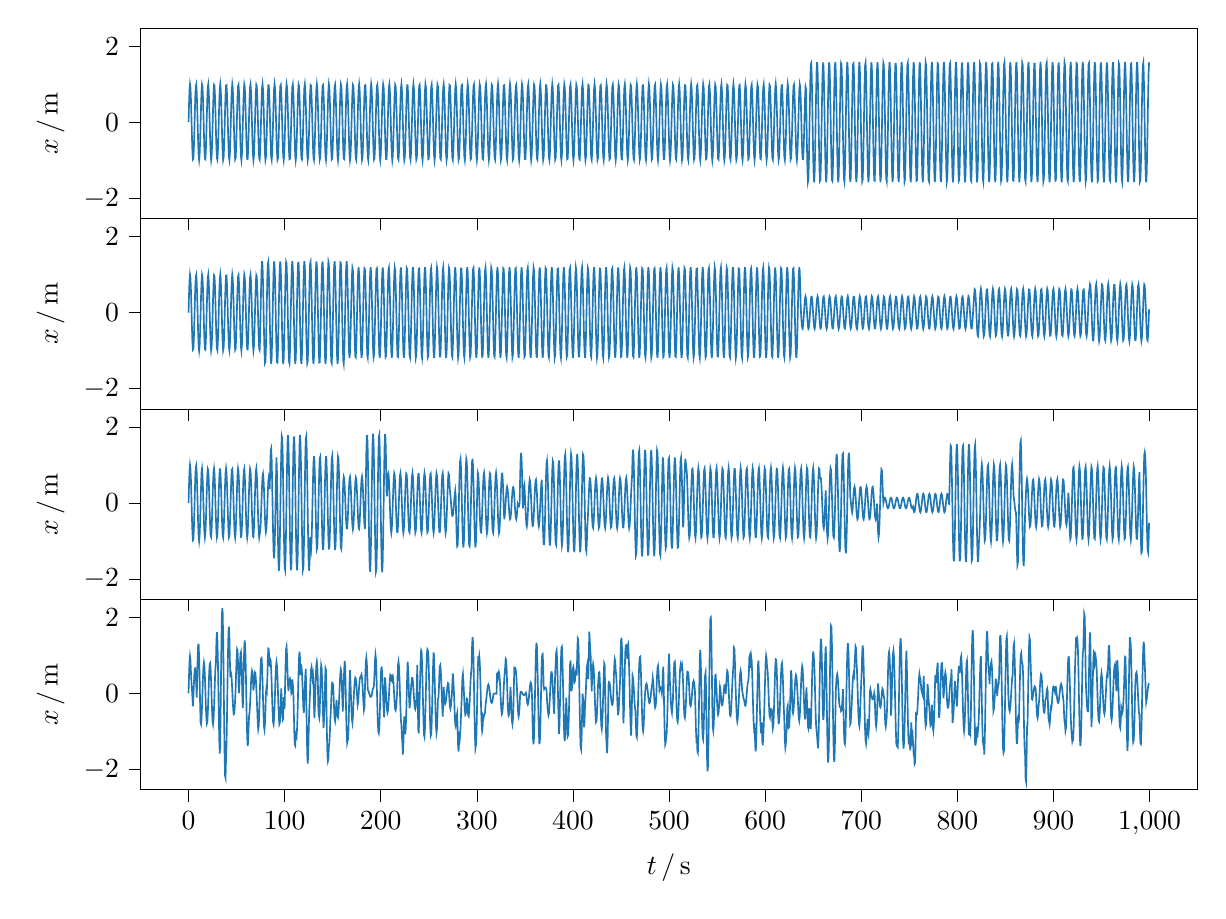
\begin{tikzpicture}

\definecolor{darkgray176}{RGB}{176,176,176}
\definecolor{steelblue31119180}{RGB}{31,119,180}

\begin{groupplot}[group style={group size=1 by 4,vertical sep=0pt,xticklabels at=edge bottom},height=4cm,width=15cm]
\nextgroupplot[
scaled x ticks=manual:{}{\pgfmathparse{#1}},
tick align=outside,
tick pos=left,
x grid style={darkgray176},
xmin=-49.975, xmax=1049.475,
xtick style={color=black},
xticklabels={},
y grid style={darkgray176},
ylabel={\(\displaystyle x\,/\,\mathrm{m}\)},
ymin=-2.53655, ymax=2.46955,
ytick style={color=black}
]
\addplot [semithick, steelblue31119180]
table {%
0 0
0.5 0.48
1 0.842
1.5 0.998
2 0.909
2.5 0.598
3 0.141
3.5 -0.351
4 -0.757
4.5 -0.978
5 -0.959
5.5 -0.705
6 -0.279
6.5 0.216
7 0.658
7.5 0.939
8 0.99
8.5 0.798
9 0.411
9.5 -0.076
10 -0.545
10.5 -0.88
11 -1
11.5 -0.875
12 -0.536
12.5 -0.065
13 0.422
13.5 0.805
14 0.991
14.5 0.935
15 0.649
15.5 0.205
16 -0.29
16.5 -0.713
17 -0.962
17.5 -0.976
18 -0.75
18.5 -0.341
19 0.152
19.5 0.607
20 0.914
20.5 0.997
21 0.836
21.5 0.47
22 -0.011
22.5 -0.489
23 -0.848
23.5 -0.999
24 -0.905
24.5 -0.589
25 -0.13
25.5 0.362
26 0.765
26.5 0.98
27 0.956
27.5 0.697
28 0.268
28.5 -0.227
29 -0.666
29.5 -0.942
30 -0.988
30.5 -0.791
31 -0.401
31.5 0.087
32 0.554
32.5 0.886
33 1
33.5 0.87
34 0.526
34.5 0.054
35 -0.432
35.5 -0.811
36 -0.993
36.5 -0.931
37 -0.641
37.5 -0.194
38 0.3
38.5 0.721
39 0.965
39.5 0.973
40 0.743
40.5 0.33
41 -0.163
41.5 -0.616
42 -0.919
42.5 -0.996
43 -0.83
43.5 -0.46
44 0.022
44.5 0.499
45 0.854
45.5 0.999
46 0.9
46.5 0.58
47 0.119
47.5 -0.372
48 -0.772
48.5 -0.982
49 -0.953
49.5 -0.689
50 -0.257
50.5 0.238
51 0.674
51.5 0.946
52 0.986
52.5 0.785
53 0.391
53.5 -0.098
54 -0.564
54.5 -0.891
55 -1
55.5 -0.864
56 -0.517
56.5 -0.043
57 0.442
57.5 0.818
58 0.994
58.5 0.926
59 0.632
59.5 0.183
60 -0.311
60.5 -0.729
61 -0.968
61.5 -0.97
62 -0.735
62.5 -0.32
63 0.174
63.5 0.625
64 0.923
64.5 0.995
65 0.823
65.5 0.45
66 -0.033
66.5 -0.509
67 -0.859
67.5 -1
68 -0.895
68.5 -0.571
69 -0.108
69.5 0.382
70 0.779
70.5 0.984
71 0.949
71.5 0.681
72 0.247
72.5 -0.248
73 -0.683
73.5 -0.95
74 -0.984
74.5 -0.778
75 -0.381
75.5 0.109
76 0.573
76.5 0.896
77 1
77.5 0.858
78 0.507
78.5 0.032
79 -0.452
79.5 -0.824
80 -0.995
80.5 -0.922
81 -0.624
81.5 -0.172
82 0.321
82.5 0.736
83 0.971
83.5 0.968
84 0.727
84.5 0.309
85 -0.185
85.5 -0.634
86 -0.927
86.5 -0.994
87 -0.817
87.5 -0.44
88 0.045
88.5 0.518
89 0.865
89.5 1
90 0.89
90.5 0.562
91 0.097
91.5 -0.393
92 -0.786
92.5 -0.986
93 -0.945
93.5 -0.673
94 -0.236
94.5 0.259
95 0.691
95.5 0.953
96 0.982
96.5 0.771
97 0.37
97.5 -0.121
98 -0.582
98.5 -0.901
99 -0.999
99.5 -0.853
100 -0.498
100.5 -0.02
101 0.462
101.5 0.831
102 0.996
102.5 0.918
103 0.615
103.5 0.161
104 -0.332
104.5 -0.744
105 -0.973
105.5 -0.965
106 -0.72
106.5 -0.299
107 0.196
107.5 0.642
108 0.931
108.5 0.992
109 0.81
109.5 0.43
110 -0.056
110.5 -0.528
111 -0.871
111.5 -1
112 -0.885
112.5 -0.553
113 -0.085
113.5 0.403
114 0.793
114.5 0.988
115 0.942
115.5 0.665
116 0.225
116.5 -0.27
117 -0.699
117.5 -0.956
118 -0.98
118.5 -0.763
119 -0.36
119.5 0.132
120 0.591
120.5 0.906
121 0.998
121.5 0.847
122 0.488
122.5 0.009
123 -0.471
123.5 -0.837
124 -0.997
124.5 -0.913
125 -0.606
125.5 -0.15
126 0.342
126.5 0.751
127 0.976
127.5 0.962
128 0.712
128.5 0.288
129 -0.207
129.5 -0.651
130 -0.935
130.5 -0.991
131 -0.804
131.5 -0.42
132 0.067
132.5 0.537
133 0.876
133.5 1
134 0.88
134.5 0.544
135 0.074
135.5 -0.413
136 -0.799
136.5 -0.99
137 -0.938
137.5 -0.656
138 -0.214
138.5 0.281
139 0.707
139.5 0.96
140 0.978
140.5 0.756
141 0.35
141.5 -0.143
142 -0.6
142.5 -0.91
143 -0.998
143.5 -0.841
144 -0.478
144.5 0.002
145 0.481
145.5 0.843
146 0.998
146.5 0.909
147 0.597
147.5 0.139
148 -0.353
148.5 -0.758
149 -0.978
149.5 -0.959
150 -0.704
150.5 -0.277
151 0.218
151.5 0.659
152 0.939
152.5 0.989
153 0.797
153.5 0.41
154 -0.078
154.5 -0.547
155 -0.881
155.5 -1
156 -0.874
156.5 -0.534
157 -0.063
157.5 0.423
158 0.806
158.5 0.991
159 0.934
159.5 0.648
160 0.203
160.5 -0.291
161 -0.714
161.5 -0.963
162 -0.975
162.5 -0.749
163 -0.339
163.5 0.154
164 0.609
164.5 0.915
165 0.997
165.5 0.835
166 0.468
166.5 -0.013
167 -0.491
167.5 -0.849
168 -0.999
168.5 -0.904
169 -0.588
169.5 -0.128
170 0.363
170.5 0.766
171 0.981
171.5 0.955
172 0.696
172.5 0.266
173 -0.228
173.5 -0.667
174 -0.943
174.5 -0.988
175 -0.79
175.5 -0.4
176 0.089
176.5 0.556
177 0.887
177.5 1
178 0.869
178.5 0.525
179 0.052
179.5 -0.433
180 -0.812
180.5 -0.993
181 -0.93
181.5 -0.639
182 -0.192
182.5 0.302
183 0.722
183.5 0.966
184 0.973
184.5 0.741
185 0.329
185.5 -0.165
186 -0.618
186.5 -0.919
187 -0.996
187.5 -0.829
188 -0.458
188.5 0.024
189 0.501
189.5 0.855
190 0.999
190.5 0.899
191 0.579
191.5 0.117
192 -0.374
192.5 -0.773
193 -0.983
193.5 -0.952
194 -0.688
194.5 -0.256
195 0.239
195.5 0.676
196 0.947
196.5 0.986
197 0.783
197.5 0.389
198 -0.1
198.5 -0.565
199 -0.892
199.5 -1
200 -0.863
200.5 -0.515
201 -0.041
201.5 0.443
202 0.819
202.5 0.994
203 0.926
203.5 0.631
204 0.181
204.5 -0.313
205 -0.73
205.5 -0.968
206 -0.97
206.5 -0.734
207 -0.318
207.5 0.176
208 0.626
208.5 0.924
209 0.995
209.5 0.822
210 0.448
210.5 -0.035
211 -0.51
211.5 -0.86
212 -1
212.5 -0.894
213 -0.57
213.5 -0.106
214 0.384
214.5 0.78
215 0.985
215.5 0.948
216 0.68
216.5 0.245
217 -0.25
217.5 -0.684
218 -0.95
218.5 -0.984
219 -0.776
219.5 -0.379
220 0.111
220.5 0.574
221 0.897
221.5 0.999
222 0.858
222.5 0.506
223 0.03
223.5 -0.453
224 -0.825
224.5 -0.995
225 -0.922
225.5 -0.622
226 -0.17
226.5 0.323
227 0.737
227.5 0.971
228 0.967
228.5 0.726
229 0.307
229.5 -0.187
230 -0.635
230.5 -0.928
231 -0.993
231.5 -0.816
232 -0.438
232.5 0.046
233 0.52
233.5 0.866
234 1
234.5 0.889
235 0.561
235.5 0.095
236 -0.394
236.5 -0.787
237 -0.987
237.5 -0.945
238 -0.672
238.5 -0.234
239 0.261
239.5 0.692
240 0.954
240.5 0.982
241 0.769
241.5 0.369
242 -0.122
242.5 -0.583
243 -0.902
243.5 -0.999
244 -0.852
244.5 -0.496
245 -0.019
245.5 0.463
246 0.832
246.5 0.996
247 0.917
247.5 0.613
248 0.159
248.5 -0.334
249 -0.745
249.5 -0.974
250 -0.964
250.5 -0.718
251 -0.297
251.5 0.198
252 0.644
252.5 0.932
253 0.992
253.5 0.809
254 0.428
254.5 -0.057
255 -0.529
255.5 -0.871
256 -1
256.5 -0.884
257 -0.551
257.5 -0.084
258 0.404
258.5 0.794
259 0.988
259.5 0.941
260 0.663
260.5 0.223
261 -0.272
261.5 -0.7
262 -0.957
262.5 -0.979
263 -0.762
263.5 -0.358
264 0.133
264.5 0.592
265 0.906
265.5 0.998
266 0.846
266.5 0.486
267 0.008
267.5 -0.473
268 -0.838
268.5 -0.997
269 -0.913
269.5 -0.604
270 -0.148
270.5 0.344
271 0.752
271.5 0.976
272 0.961
272.5 0.711
273 0.286
273.5 -0.208
274 -0.652
274.5 -0.936
275 -0.991
275.5 -0.803
276 -0.418
276.5 0.069
277 0.539
277.5 0.877
278 1
278.5 0.879
279 0.542
279.5 0.073
280 -0.415
280.5 -0.8
281 -0.99
281.5 -0.937
282 -0.655
282.5 -0.212
283 0.282
283.5 0.708
284 0.96
284.5 0.977
285 0.755
285.5 0.348
286 -0.144
286.5 -0.601
287 -0.911
287.5 -0.998
288 -0.84
288.5 -0.476
289 0.004
289.5 0.483
290 0.844
290.5 0.998
291 0.908
291.5 0.596
292 0.137
292.5 -0.355
293 -0.76
293.5 -0.979
294 -0.958
294.5 -0.703
295 -0.275
295.5 0.219
296 0.66
296.5 0.94
297 0.989
297.5 0.796
298 0.408
298.5 -0.08
299 -0.548
299.5 -0.882
300 -1
300.5 -0.873
301 -0.533
301.5 -0.061
302 0.425
302.5 0.807
303 0.992
303.5 0.933
304 0.647
304.5 0.201
305 -0.293
305.5 -0.716
306 -0.963
306.5 -0.975
307 -0.748
307.5 -0.337
308 0.155
308.5 0.61
309 0.916
309.5 0.997
310 0.834
310.5 0.467
311 -0.015
311.5 -0.493
312 -0.85
312.5 -0.999
313 -0.903
313.5 -0.587
314 -0.126
314.5 0.365
315 0.767
315.5 0.981
316 0.955
316.5 0.695
317 0.265
317.5 -0.23
318 -0.669
318.5 -0.944
319 -0.987
319.5 -0.789
320 -0.398
320.5 0.091
321 0.557
321.5 0.887
322 1
322.5 0.868
323 0.523
323.5 0.05
324 -0.435
324.5 -0.814
325 -0.993
325.5 -0.929
326 -0.638
326.5 -0.191
327 0.304
327.5 0.723
328 0.966
328.5 0.972
329 0.74
329.5 0.327
330 -0.166
330.5 -0.619
331 -0.92
331.5 -0.996
332 -0.828
332.5 -0.457
333 0.026
333.5 0.502
334 0.855
334.5 0.999
335 0.898
335.5 0.578
336 0.115
336.5 -0.375
337 -0.774
337.5 -0.983
338 -0.951
338.5 -0.687
339 -0.254
339.5 0.241
340 0.677
340.5 0.947
341 0.985
341.5 0.782
342 0.388
342.5 -0.102
343 -0.567
343.5 -0.892
344 -1
344.5 -0.862
345 -0.514
345.5 -0.039
346 0.445
346.5 0.82
347 0.994
347.5 0.925
348 0.629
348.5 0.18
349 -0.314
349.5 -0.731
350 -0.969
350.5 -0.969
351 -0.733
351.5 -0.316
352 0.177
352.5 0.628
353 0.924
353.5 0.995
354 0.821
354.5 0.447
355 -0.037
355.5 -0.512
356 -0.861
356.5 -1
357 -0.893
357.5 -0.568
358 -0.104
358.5 0.386
359 0.781
359.5 0.985
360 0.948
360.5 0.679
361 0.243
361.5 -0.252
362 -0.685
362.5 -0.951
363 -0.983
363.5 -0.775
364 -0.377
364.5 0.113
365 0.576
365.5 0.897
366 0.999
366.5 0.857
367 0.504
367.5 0.028
368 -0.455
368.5 -0.826
369 -0.995
369.5 -0.921
370 -0.621
370.5 -0.169
371 0.325
371.5 0.739
372 0.972
372.5 0.967
373 0.725
373.5 0.306
374 -0.188
374.5 -0.636
375 -0.928
375.5 -0.993
376 -0.815
376.5 -0.437
377 0.048
377.5 0.521
378 0.867
378.5 1
379 0.888
379.5 0.559
380 0.093
380.5 -0.396
381 -0.788
381.5 -0.987
382 -0.944
382.5 -0.67
383 -0.232
383.5 0.263
384 0.693
384.5 0.954
385 0.981
385.5 0.768
386 0.367
386.5 -0.124
387 -0.585
387.5 -0.902
388 -0.999
388.5 -0.851
389 -0.494
389.5 -0.017
390 0.465
390.5 0.833
391 0.996
391.5 0.916
392 0.612
392.5 0.158
393 -0.335
393.5 -0.746
394 -0.974
394.5 -0.964
395 -0.717
395.5 -0.295
396 0.199
396.5 0.645
397 0.933
397.5 0.992
398 0.808
398.5 0.427
399 -0.059
399.5 -0.531
400 -0.872
400.5 -1
401 -0.883
401.5 -0.55
402 -0.082
402.5 0.406
403 0.795
403.5 0.989
404 0.941
404.5 0.662
405 0.221
405.5 -0.273
406 -0.701
406.5 -0.957
407 -0.979
407.5 -0.761
408 -0.357
408.5 0.135
409 0.594
409.5 0.907
410 0.998
410.5 0.845
411 0.485
411.5 0.006
412 -0.475
412.5 -0.839
413 -0.997
413.5 -0.912
414 -0.603
414.5 -0.147
415 0.346
415.5 0.754
416 0.977
416.5 0.961
417 0.709
417.5 0.284
418 -0.21
418.5 -0.653
419 -0.937
419.5 -0.99
420 -0.802
420.5 -0.417
421 0.07
421.5 0.54
422 0.878
422.5 1
423 0.878
423.5 0.541
424 0.071
424.5 -0.416
425 -0.801
425.5 -0.99
426 -0.937
426.5 -0.654
427 -0.211
427.5 0.284
428 0.709
428.5 0.961
429 0.977
429.5 0.754
430 0.346
430.5 -0.146
431 -0.603
431.5 -0.912
432 -0.997
432.5 -0.839
433 -0.475
433.5 0.005
434 0.484
434.5 0.845
435 0.998
435.5 0.907
436 0.594
436.5 0.136
437 -0.356
437.5 -0.761
438 -0.979
438.5 -0.958
439 -0.702
439.5 -0.274
440 0.221
440.5 0.662
441 0.94
441.5 0.989
442 0.795
442.5 0.406
443 -0.082
443.5 -0.55
444 -0.883
444.5 -1
445 -0.873
445.5 -0.531
446 -0.06
446.5 0.426
447 0.808
447.5 0.992
448 0.933
448.5 0.645
449 0.2
449.5 -0.295
450 -0.717
450.5 -0.964
451 -0.974
451.5 -0.746
452 -0.336
452.5 0.157
453 0.612
453.5 0.916
454 0.997
454.5 0.833
455 0.465
455.5 -0.017
456 -0.494
456.5 -0.851
457 -0.999
457.5 -0.902
458 -0.585
458.5 -0.124
459 0.367
459.5 0.768
460 0.981
460.5 0.954
461 0.694
461.5 0.263
462 -0.232
462.5 -0.67
463 -0.944
463.5 -0.987
464 -0.788
464.5 -0.396
465 0.093
465.5 0.559
466 0.888
466.5 1
467 0.867
467.5 0.522
468 0.049
468.5 -0.436
469 -0.815
469.5 -0.993
470 -0.929
470.5 -0.637
471 -0.189
471.5 0.305
472 0.725
472.5 0.967
473 0.972
473.5 0.739
474 0.325
474.5 -0.168
475 -0.62
475.5 -0.921
476 -0.995
476.5 -0.827
477 -0.455
477.5 0.028
478 0.504
478.5 0.856
479 0.999
479.5 0.898
480 0.576
480.5 0.113
481 -0.377
481.5 -0.775
482 -0.983
482.5 -0.951
483 -0.685
483.5 -0.252
484 0.243
484.5 0.678
485 0.948
485.5 0.985
486 0.781
486.5 0.386
487 -0.104
487.5 -0.568
488 -0.893
488.5 -1
489 -0.861
489.5 -0.512
490 -0.037
490.5 0.446
491 0.821
491.5 0.994
492 0.924
492.5 0.628
493 0.178
493.5 -0.316
494 -0.732
494.5 -0.969
495 -0.969
495.5 -0.731
496 -0.315
496.5 0.179
497 0.629
497.5 0.925
498 0.994
498.5 0.82
499 0.445
499.5 -0.039
500 -0.513
500.5 -0.862
501 -1
501.5 -0.893
502 -0.567
502.5 -0.102
503 0.387
503.5 0.782
504 0.985
504.5 0.947
505 0.677
505.5 0.241
506 -0.254
506.5 -0.686
507 -0.951
507.5 -0.983
508 -0.774
508.5 -0.376
509 0.115
509.5 0.577
510 0.898
510.5 0.999
511 0.856
511.5 0.503
512 0.026
512.5 -0.456
513 -0.827
513.5 -0.996
514 -0.92
514.5 -0.619
515 -0.167
515.5 0.327
516 0.74
516.5 0.972
517 0.966
517.5 0.724
518 0.304
518.5 -0.19
519 -0.638
519.5 -0.929
520 -0.993
520.5 -0.814
521 -0.435
521.5 0.05
522 0.523
522.5 0.868
523 1
523.5 0.888
524 0.558
524.5 0.091
525 -0.398
525.5 -0.789
526 -0.987
526.5 -0.944
527 -0.669
527.5 -0.231
528 0.264
528.5 0.695
529 0.955
529.5 0.981
530 0.767
530.5 0.365
531 -0.126
531.5 -0.586
532 -0.903
532.5 -0.999
533 -0.85
533.5 -0.493
534 -0.015
534.5 0.466
535 0.834
535.5 0.997
536 0.916
536.5 0.61
537 0.156
537.5 -0.337
538 -0.747
538.5 -0.975
539 -0.963
539.5 -0.716
540 -0.293
540.5 0.201
541 0.646
541.5 0.933
542 0.992
542.5 0.807
543 0.425
543.5 -0.061
544 -0.532
544.5 -0.873
545 -1
545.5 -0.882
546 -0.548
546.5 -0.08
547 0.408
547.5 0.796
548 0.989
548.5 0.94
549 0.661
549.5 0.22
550 -0.275
550.5 -0.703
551 -0.958
551.5 -0.979
552 -0.76
552.5 -0.355
553 0.137
553.5 0.595
554 0.908
554.5 0.998
555 0.844
555.5 0.483
556 0.004
556.5 -0.476
557 -0.84
557.5 -0.998
558 -0.911
558.5 -0.602
559 -0.145
559.5 0.348
560 0.755
560.5 0.977
561 0.96
561.5 0.708
562 0.283
562.5 -0.212
563 -0.655
563.5 -0.937
564 -0.99
564.5 -0.801
565 -0.415
565.5 0.072
566 0.542
566.5 0.879
567 1
567.5 0.877
568 0.539
568.5 0.069
569 -0.418
569.5 -0.803
570 -0.991
570.5 -0.936
571 -0.652
571.5 -0.209
572 0.286
572.5 0.71
573 0.961
573.5 0.976
574 0.753
574.5 0.345
575 -0.148
575.5 -0.604
576 -0.912
576.5 -0.997
577 -0.838
577.5 -0.473
578 0.007
578.5 0.486
579 0.846
579.5 0.998
580 0.906
580.5 0.593
581 0.134
581.5 -0.358
582 -0.762
582.5 -0.979
583 -0.957
583.5 -0.7
584 -0.272
584.5 0.223
585 0.663
585.5 0.941
586 0.988
586.5 0.794
587 0.405
587.5 -0.083
588 -0.551
588.5 -0.884
589 -1
589.5 -0.872
590 -0.53
590.5 -0.058
591 0.428
591.5 0.809
592 0.992
592.5 0.932
593 0.644
593.5 0.198
594 -0.296
594.5 -0.718
595 -0.964
595.5 -0.974
596 -0.745
596.5 -0.334
597 0.159
597.5 0.613
598 0.917
598.5 0.996
599 0.832
599.5 0.463
600 -0.018
600.5 -0.496
601 -0.852
601.5 -0.999
602 -0.902
602.5 -0.584
603 -0.123
603.5 0.368
604 0.769
604.5 0.982
605 0.954
605.5 0.692
606 0.261
606.5 -0.234
607 -0.671
607.5 -0.945
608 -0.987
608.5 -0.787
609 -0.395
609.5 0.094
610 0.56
610.5 0.889
611 1
611.5 0.866
612 0.52
612.5 0.047
613 -0.438
613.5 -0.816
614 -0.993
614.5 -0.928
615 -0.635
615.5 -0.187
616 0.307
616.5 0.726
617 0.967
617.5 0.971
618 0.738
618.5 0.323
619 -0.17
619.5 -0.622
620 -0.921
620.5 -0.995
621 -0.826
621.5 -0.454
622 0.029
622.5 0.505
623 0.857
623.5 0.999
624 0.897
624.5 0.575
625 0.112
625.5 -0.379
626 -0.776
626.5 -0.984
627 -0.95
627.5 -0.684
628 -0.25
628.5 0.245
629 0.68
629.5 0.948
630 0.985
630.5 0.78
631 0.384
631.5 -0.106
632 -0.57
632.5 -0.894
633 -1
633.5 -0.86
634 -0.511
634.5 -0.036
635 0.448
635.5 0.822
636 0.995
636.5 0.924
637 0.627
637.5 0.176
638 -0.318
638.5 -0.734
639 -0.97
639.5 -0.969
640 -0.73
640.5 -0.313
641 0.181
641.5 0.63
642 0.926
642.5 0.873
643 0.132
643.5 -0.641
644 -1.257
644.5 -1.565
645 -1.49
645.5 -1.05
646 -0.353
646.5 0.431
647 1.109
647.5 1.516
648 1.551
648.5 1.207
649 0.567
649.5 -0.212
650 -0.939
650.5 -1.436
651 -1.581
651.5 -1.339
652 -0.769
652.5 -0.011
653 0.75
653.5 1.327
654 1.579
654.5 1.445
655 0.957
655.5 0.234
656 -0.546
656.5 -1.192
657 -1.546
657.5 -1.522
658 -1.125
658.5 -0.453
659 0.331
659.5 1.033
660 1.482
660.5 1.569
661 1.271
661.5 0.662
662 -0.109
662.5 -0.854
663 -1.389
663.5 -1.584
664 -1.391
664.5 -0.858
665 -0.114
665.5 0.657
666 1.268
666.5 1.568
667 1.484
667.5 1.037
668 0.336
668.5 -0.448
669 -1.121
669.5 -1.521
670 -1.547
670.5 -1.195
671 -0.55
671.5 0.229
672 0.953
672.5 1.443
673 1.58
673.5 1.33
674 0.754
674.5 -0.006
675 -0.765
675.5 -1.336
676 -1.581
676.5 -1.438
677 -0.943
677.5 -0.217
678 0.562
678.5 1.203
679 1.55
679.5 1.517
680 1.112
680.5 0.436
681 -0.348
681.5 -1.046
682 -1.488
682.5 -1.566
683 -1.26
683.5 -0.646
684 0.127
684.5 0.868
685 1.397
685.5 1.584
686 1.383
686.5 0.843
687 0.097
687.5 -0.673
688 -1.278
688.5 -1.57
689 -1.478
689.5 -1.023
690 -0.318
690.5 0.465
691 1.134
691.5 1.525
692 1.543
692.5 1.183
693 0.534
693.5 -0.247
694 -0.967
694.5 -1.45
695 -1.578
695.5 -1.32
696 -0.738
696.5 0.024
697 0.78
697.5 1.346
698 1.582
698.5 1.43
699 0.928
699.5 0.199
700 -0.579
700.5 -1.215
701 -1.554
701.5 -1.512
702 -1.1
702.5 -0.419
703 0.365
703.5 1.06
704 1.494
704.5 1.563
705 1.249
705.5 0.63
706 -0.145
706.5 -0.883
707 -1.406
707.5 -1.584
708 -1.374
708.5 -0.828
709 -0.079
709.5 0.689
710 1.289
710.5 1.573
711 1.471
711.5 1.01
712 0.301
712.5 -0.482
713 -1.146
713.5 -1.53
714 -1.539
714.5 -1.172
715 -0.517
715.5 0.264
716 0.981
716.5 1.457
717 1.577
717.5 1.31
718 0.723
718.5 -0.042
719 -0.796
719.5 -1.355
720 -1.583
720.5 -1.422
721 -0.914
721.5 -0.182
722 0.595
722.5 1.226
723 1.557
723.5 1.506
724 1.087
724.5 0.402
725 -0.382
725.5 -1.073
726 -1.5
726.5 -1.56
727 -1.238
727.5 -0.613
728 0.162
728.5 0.898
729 1.414
729.5 1.583
730 1.365
730.5 0.813
731 0.061
731.5 -0.705
732 -1.299
732.5 -1.575
733 -1.465
733.5 -0.996
734 -0.284
734.5 0.498
735 1.158
735.5 1.535
736 1.535
736.5 1.16
737 0.5
737.5 -0.282
738 -0.995
738.5 -1.464
739 -1.575
739.5 -1.3
740 -0.707
740.5 0.059
741 0.811
741.5 1.364
742 1.583
742.5 1.415
743 0.9
743.5 0.164
744 -0.611
744.5 -1.237
745 -1.56
745.5 -1.501
746 -1.074
746.5 -0.384
747 0.399
747.5 1.086
748 1.506
748.5 1.557
749 1.227
749.5 0.597
750 -0.18
750.5 -0.912
751 -1.421
751.5 -1.583
752 -1.356
752.5 -0.798
753 -0.044
753.5 0.721
754 1.309
754.5 1.576
755 1.458
755.5 0.982
756 0.266
756.5 -0.515
757 -1.17
757.5 -1.539
758 -1.531
758.5 -1.148
759 -0.484
759.5 0.299
760 1.008
760.5 1.471
761 1.573
761.5 1.29
762 0.691
762.5 -0.077
763 -0.826
763.5 -1.373
764 -1.584
764.5 -1.407
765 -0.885
765.5 -0.147
766 0.628
766.5 1.248
767 1.563
767.5 1.495
768 1.061
768.5 0.367
769 -0.417
769.5 -1.098
770 -1.511
770.5 -1.554
771 -1.216
771.5 -0.581
772 0.197
772.5 0.927
773 1.429
773.5 1.582
774 1.347
774.5 0.782
775 0.026
775.5 -0.736
776 -1.319
776.5 -1.578
777 -1.451
777.5 -0.968
778 -0.249
778.5 0.532
779 1.182
779.5 1.543
780 1.526
780.5 1.135
781 0.467
781.5 -0.316
782 -1.022
782.5 -1.477
783 -1.571
783.5 -1.28
784 -0.675
784.5 0.095
785 0.841
785.5 1.382
786 1.584
786.5 1.398
787 0.87
787.5 0.129
788 -0.644
788.5 -1.259
789 -1.566
789.5 -1.489
790 -1.048
790.5 -0.35
791 0.434
791.5 1.111
792 1.516
792.5 1.55
793 1.205
793.5 0.564
794 -0.215
794.5 -0.941
795 -1.437
795.5 -1.581
796 -1.338
796.5 -0.767
797 -0.008
797.5 0.752
798 1.328
798.5 1.579
799 1.444
799.5 0.954
800 0.231
800.5 -0.548
801 -1.194
801.5 -1.547
802 -1.521
802.5 -1.123
803 -0.45
803.5 0.334
804 1.035
804.5 1.483
805 1.568
805.5 1.269
806 0.659
806.5 -0.112
807 -0.856
807.5 -1.39
808 -1.584
808.5 -1.39
809 -0.855
809.5 -0.111
810 0.66
810.5 1.27
811 1.568
811.5 1.483
812 1.035
812.5 0.333
813 -0.45
813.5 -1.123
814 -1.521
814.5 -1.547
815 -1.193
815.5 -0.548
816 0.232
816.5 0.955
817 1.444
817.5 1.579
818 1.328
818.5 0.751
819 -0.009
819.5 -0.768
820 -1.338
820.5 -1.581
821 -1.436
821.5 -0.94
822 -0.214
822.5 0.565
823 1.205
823.5 1.551
824 1.516
824.5 1.11
825 0.433
825.5 -0.351
826 -1.048
826.5 -1.489
827 -1.566
827.5 -1.258
828 -0.643
828.5 0.13
829 0.871
829.5 1.399
830 1.584
830.5 1.381
831 0.841
831.5 0.094
832 -0.676
832.5 -1.28
833 -1.571
833.5 -1.477
834 -1.021
834.5 -0.316
835 0.467
835.5 1.136
836 1.526
836.5 1.543
837 1.182
837.5 0.531
838 -0.25
838.5 -0.969
839 -1.451
839.5 -1.578
840 -1.318
840.5 -0.736
841 0.027
841.5 0.783
842 1.347
842.5 1.582
843 1.429
843.5 0.926
844 0.196
844.5 -0.581
845 -1.217
845.5 -1.554
846 -1.511
846.5 -1.098
847 -0.416
847.5 0.368
848 1.062
848.5 1.495
849 1.563
849.5 1.248
850 0.627
850.5 -0.147
851 -0.886
851.5 -1.407
852 -1.584
852.5 -1.373
853 -0.826
853.5 -0.076
854 0.692
854.5 1.29
855 1.573
855.5 1.47
856 1.008
856.5 0.298
857 -0.484
857.5 -1.148
858 -1.531
858.5 -1.539
859 -1.17
859.5 -0.514
860 0.267
860.5 0.983
861 1.458
861.5 1.576
862 1.308
862.5 0.72
863 -0.044
863.5 -0.798
864 -1.357
864.5 -1.583
865 -1.421
865.5 -0.912
866 -0.179
866.5 0.598
867 1.228
867.5 1.557
868 1.506
868.5 1.085
869 0.399
869.5 -0.385
870 -1.075
870.5 -1.501
871 -1.56
871.5 -1.237
872 -0.611
872.5 0.165
873 0.9
873.5 1.415
874 1.583
874.5 1.364
875 0.81
875.5 0.059
876 -0.708
876.5 -1.3
877 -1.575
877.5 -1.464
878 -0.994
878.5 -0.281
879 0.501
879.5 1.16
880 1.535
880.5 1.534
881 1.158
881.5 0.498
882 -0.284
882.5 -0.997
883 -1.465
883.5 -1.575
884 -1.298
884.5 -0.704
885 0.062
885.5 0.813
886 1.366
886.5 1.583
887 1.413
887.5 0.897
888 0.161
888.5 -0.614
889 -1.239
889.5 -1.561
890 -1.5
890.5 -1.072
891 -0.382
891.5 0.402
892 1.088
892.5 1.507
893 1.557
893.5 1.226
894 0.594
894.5 -0.182
895 -0.915
895.5 -1.423
896 -1.582
896.5 -1.355
897 -0.795
897.5 -0.041
898 0.723
898.5 1.31
899 1.577
899.5 1.457
900 0.98
900.5 0.263
901 -0.518
901.5 -1.172
902 -1.54
902.5 -1.53
903 -1.146
903.5 -0.481
904 0.302
904.5 1.01
905 1.472
905.5 1.572
906 1.288
906.5 0.689
907 -0.08
907.5 -0.829
908 -1.374
908.5 -1.584
909 -1.405
909.5 -0.883
910 -0.144
910.5 0.63
911 1.25
911.5 1.563
912 1.494
912.5 1.059
913 0.365
913.5 -0.419
914 -1.1
914.5 -1.512
915 -1.553
915.5 -1.214
916 -0.578
916.5 0.2
917 0.929
917.5 1.43
918 1.582
918.5 1.345
919 0.78
919.5 0.023
920 -0.739
920.5 -1.32
921 -1.578
921.5 -1.45
922 -0.966
922.5 -0.246
923 0.534
923.5 1.184
924 1.544
924.5 1.525
925 1.133
925.5 0.464
926 -0.319
926.5 -1.024
927 -1.478
927.5 -1.57
928 -1.278
928.5 -0.673
929 0.097
929.5 0.844
930 1.383
930.5 1.584
931 1.397
931.5 0.868
932 0.126
932.5 -0.646
933 -1.261
933.5 -1.566
934 -1.488
934.5 -1.046
935 -0.347
935.5 0.436
936 1.113
936.5 1.517
937 1.55
937.5 1.203
938 0.561
938.5 -0.217
939 -0.943
939.5 -1.438
940 -1.581
940.5 -1.336
941 -0.764
941.5 -0.006
942 0.755
942.5 1.33
943 1.58
943.5 1.443
944 0.952
944.5 0.229
945 -0.551
945.5 -1.196
946 -1.547
946.5 -1.52
947 -1.121
947.5 -0.447
948 0.336
948.5 1.037
949 1.484
949.5 1.568
950 1.267
950.5 0.657
951 -0.115
951.5 -0.858
952 -1.392
952.5 -1.584
953 -1.389
953.5 -0.853
954 -0.109
954.5 0.662
955 1.271
955.5 1.569
956 1.482
956.5 1.032
957 0.33
957.5 -0.453
958 -1.125
958.5 -1.522
959 -1.546
959.5 -1.191
960 -0.545
960.5 0.235
961 0.957
961.5 1.445
962 1.579
962.5 1.327
963 0.749
963.5 -0.012
964 -0.77
964.5 -1.339
965 -1.581
965.5 -1.435
966 -0.938
966.5 -0.211
967 0.567
967.5 1.207
968 1.551
968.5 1.515
969 1.108
969.5 0.43
970 -0.354
970.5 -1.051
971 -1.49
971.5 -1.565
972 -1.257
972.5 -0.64
973 0.133
973.5 0.873
974 1.4
974.5 1.584
975 1.38
975.5 0.838
976 0.091
976.5 -0.678
977 -1.282
977.5 -1.571
978 -1.476
978.5 -1.019
979 -0.313
979.5 0.47
980 1.138
980.5 1.527
981 1.542
981.5 1.18
982 0.528
982.5 -0.252
983 -0.971
983.5 -1.452
984 -1.578
984.5 -1.317
985 -0.733
985.5 0.03
986 0.785
986.5 1.349
987 1.582
987.5 1.428
988 0.924
988.5 0.194
989 -0.584
989.5 -1.218
990 -1.555
990.5 -1.51
991 -1.096
991.5 -0.413
992 0.371
992.5 1.064
993 1.496
993.5 1.562
994 1.246
994.5 0.624
995 -0.15
995.5 -0.888
996 -1.408
996.5 -1.584
997 -1.371
997.5 -0.823
998 -0.073
998.5 0.694
999 1.292
999.5 1.573
};

\nextgroupplot[
scaled x ticks=manual:{}{\pgfmathparse{#1}},
tick align=outside,
tick pos=left,
x grid style={darkgray176},
xmin=-49.975, xmax=1049.475,
xtick style={color=black},
xticklabels={},
y grid style={darkgray176},
ylabel={\(\displaystyle x\,/\,\mathrm{m}\)},
ymin=-2.53655, ymax=2.46955,
ytick style={color=black}
]
\addplot [semithick, steelblue31119180]
table {%
0 0
0.5 0.48
1 0.842
1.5 0.998
2 0.909
2.5 0.598
3 0.141
3.5 -0.351
4 -0.757
4.5 -0.978
5 -0.959
5.5 -0.705
6 -0.279
6.5 0.216
7 0.658
7.5 0.939
8 0.99
8.5 0.798
9 0.411
9.5 -0.076
10 -0.545
10.5 -0.88
11 -1
11.5 -0.875
12 -0.536
12.5 -0.065
13 0.422
13.5 0.805
14 0.991
14.5 0.935
15 0.649
15.5 0.205
16 -0.29
16.5 -0.713
17 -0.962
17.5 -0.976
18 -0.75
18.5 -0.341
19 0.152
19.5 0.607
20 0.914
20.5 0.997
21 0.836
21.5 0.47
22 -0.011
22.5 -0.489
23 -0.848
23.5 -0.999
24 -0.905
24.5 -0.589
25 -0.13
25.5 0.362
26 0.765
26.5 0.98
27 0.956
27.5 0.697
28 0.268
28.5 -0.227
29 -0.666
29.5 -0.942
30 -0.988
30.5 -0.791
31 -0.401
31.5 0.087
32 0.554
32.5 0.886
33 1
33.5 0.87
34 0.526
34.5 0.054
35 -0.432
35.5 -0.811
36 -0.993
36.5 -0.931
37 -0.641
37.5 -0.194
38 0.3
38.5 0.721
39 0.965
39.5 0.973
40 0.743
40.5 0.33
41 -0.163
41.5 -0.616
42 -0.919
42.5 -0.996
43 -0.83
43.5 -0.46
44 0.022
44.5 0.499
45 0.854
45.5 0.999
46 0.9
46.5 0.58
47 0.119
47.5 -0.372
48 -0.772
48.5 -0.982
49 -0.953
49.5 -0.689
50 -0.257
50.5 0.238
51 0.674
51.5 0.946
52 0.986
52.5 0.785
53 0.391
53.5 -0.098
54 -0.564
54.5 -0.891
55 -1
55.5 -0.864
56 -0.517
56.5 -0.043
57 0.442
57.5 0.818
58 0.994
58.5 0.926
59 0.632
59.5 0.183
60 -0.311
60.5 -0.729
61 -0.968
61.5 -0.97
62 -0.735
62.5 -0.32
63 0.174
63.5 0.625
64 0.923
64.5 0.995
65 0.823
65.5 0.45
66 -0.033
66.5 -0.509
67 -0.859
67.5 -1
68 -0.895
68.5 -0.571
69 -0.108
69.5 0.382
70 0.779
70.5 0.984
71 0.949
71.5 0.681
72 0.247
72.5 -0.248
73 -0.683
73.5 -0.95
74 -0.984
74.5 -0.633
75 0.018
75.5 0.665
76 1.148
76.5 1.351
77 1.223
77.5 0.795
78 0.173
78.5 -0.492
79 -1.036
79.5 -1.327
80 -1.292
80.5 -0.941
81 -0.36
81.5 0.31
82 0.903
82.5 1.276
83 1.336
83.5 1.069
84 0.54
84.5 -0.121
85 -0.752
85.5 -1.2
86 -1.353
86.5 -1.175
87 -0.709
87.5 -0.07
88 0.587
88.5 1.099
89 1.343
89.5 1.258
90 0.864
90.5 0.259
91 -0.409
91.5 -0.977
92 -1.306
92.5 -1.316
93 -1.002
93.5 -0.444
94 0.223
94.5 0.836
95 1.244
95.5 1.347
96 1.12
96.5 0.619
97 -0.033
97.5 -0.678
98 -1.156
98.5 -1.352
99 -1.216
99.5 -0.783
100 -0.158
100.5 0.506
101 1.046
101.5 1.329
102 1.288
102.5 0.93
103 0.345
103.5 -0.324
104 -0.915
104.5 -1.281
105 -1.333
105.5 -1.059
106 -0.526
106.5 0.136
107 0.765
107.5 1.206
108 1.353
108.5 1.167
109 0.696
109.5 0.055
110 -0.6
110.5 -1.108
111 -1.345
111.5 -1.252
112 -0.853
112.5 -0.245
113 0.423
113.5 0.988
114 1.31
114.5 1.312
115 0.992
115.5 0.43
116 -0.238
116.5 -0.848
117 -1.25
117.5 -1.346
118 -1.112
118.5 -0.606
119 0.048
119.5 0.691
120 1.164
120.5 1.352
121 1.209
121.5 0.77
122 0.143
122.5 -0.52
123 -1.055
123.5 -1.332
124 -1.283
124.5 -0.919
125 -0.331
125.5 0.339
126 0.926
126.5 1.286
127 1.331
127.5 1.05
128 0.512
128.5 -0.151
129 -0.777
129.5 -1.213
130 -1.352
130.5 -1.16
131 -0.683
131.5 -0.04
132 0.614
132.5 1.117
133 1.346
133.5 1.246
134 0.841
134.5 0.23
135 -0.438
135.5 -0.998
136 -1.314
136.5 -1.308
137 -0.982
137.5 -0.415
138 0.253
138.5 0.859
139 1.255
139.5 1.344
140 1.103
140.5 0.593
141 -0.063
141.5 -0.704
142 -1.172
142.5 -1.353
143 -1.203
143.5 -0.758
144 -0.128
144.5 0.534
145 1.065
145.5 1.335
146 1.278
146.5 0.908
147 0.316
147.5 -0.354
148 -0.937
148.5 -1.29
149 -1.328
149.5 -1.04
150 -0.498
150.5 0.166
151 0.79
151.5 1.22
152 1.351
152.5 1.152
153 0.67
153.5 0.025
154 -0.627
154.5 -1.125
155 -1.348
155.5 -1.24
156 -0.829
156.5 -0.215
157 0.452
157.5 1.008
158 1.317
158.5 1.304
159 0.972
159.5 0.401
160 -0.268
160.5 -0.871
161 -1.261
161.5 -1.342
162 -1.094
162.5 -0.579
163 0.078
163.5 0.717
164 1.179
164.5 1.353
165 1.196
165.5 0.745
166 0.113
166.5 -0.548
167 -1.038
167.5 -1.192
168 -1.054
168.5 -0.658
169 -0.101
169.5 0.481
170 0.945
170.5 1.178
171 1.122
171.5 0.791
172 0.267
172.5 -0.323
173 -0.834
173.5 -1.14
174 -1.168
174.5 -0.909
175 -0.428
175.5 0.158
176 0.705
176.5 1.08
177 1.19
177.5 1.009
178 0.58
178.5 0.01
179 -0.563
179.5 -0.998
180 -1.188
180.5 -1.088
181 -0.721
181.5 -0.178
182 0.409
182.5 0.896
183 1.163
183.5 1.146
184 0.848
184.5 0.342
185 -0.247
185.5 -0.776
186 -1.115
186.5 -1.181
187 -0.957
187.5 -0.499
188 0.081
188.5 0.641
189 1.045
189.5 1.192
190 1.048
190.5 0.647
191 0.088
191.5 -0.493
192 -0.953
192.5 -1.18
193 -1.117
193.5 -0.781
194 -0.254
194.5 0.336
195 0.843
195.5 1.144
196 1.165
196.5 0.9
197 0.416
197.5 -0.171
198 -0.716
198.5 -1.085
199 -1.189
199.5 -1.002
200 -0.569
200.5 0.003
201 0.574
201.5 1.005
202 1.189
202.5 1.083
203 0.711
203.5 0.165
204 -0.422
204.5 -0.905
205 -1.166
205.5 -1.142
206 -0.838
206.5 -0.329
207 0.26
207.5 0.786
208 1.12
208.5 1.179
209 0.949
209.5 0.487
210 -0.094
210.5 -0.652
211 -1.051
211.5 -1.192
212 -1.041
212.5 -0.636
213 -0.074
213.5 0.505
214 0.961
214.5 1.182
215 1.113
215.5 0.771
216 0.241
216.5 -0.348
217 -0.852
217.5 -1.148
218 -1.162
218.5 -0.892
219 -0.403
219.5 0.184
220 0.726
220.5 1.091
221 1.188
221.5 0.994
222 0.557
222.5 -0.017
223 -0.586
223.5 -1.012
224 -1.19
224.5 -1.077
225 -0.7
225.5 -0.152
226 0.434
226.5 0.913
227 1.169
227.5 1.138
228 0.829
228.5 0.317
229 -0.273
229.5 -0.796
230 -1.124
230.5 -1.177
231 -0.941
231.5 -0.475
232 0.107
232.5 0.663
233 1.057
233.5 1.192
234 1.035
234.5 0.624
235 0.061
235.5 -0.517
236 -0.969
236.5 -1.183
237 -1.108
237.5 -0.761
238 -0.228
238.5 0.361
239 0.862
239.5 1.151
240 1.159
240.5 0.883
241 0.391
241.5 -0.197
242 -0.737
242.5 -1.096
243 -1.187
243.5 -0.987
244 -0.545
244.5 0.03
245 0.598
245.5 1.019
246 1.191
246.5 1.071
247 0.689
247.5 0.138
248 -0.446
248.5 -0.922
249 -1.171
249.5 -1.134
250 -0.819
250.5 -0.304
251 0.286
251.5 0.806
252 1.129
252.5 1.175
253 0.933
253.5 0.463
254 -0.12
254.5 -0.674
255 -1.063
255.5 -1.192
256 -1.028
256.5 -0.613
257 -0.048
257.5 0.529
258 0.977
258.5 1.185
259 1.103
259.5 0.751
260 0.215
260.5 -0.374
261 -0.871
261.5 -1.155
262 -1.156
262.5 -0.874
263 -0.378
263.5 0.21
264 0.747
264.5 1.101
265 1.185
265.5 0.979
266 0.533
266.5 -0.043
267 -0.609
267.5 -1.026
268 -1.192
268.5 -1.065
269 -0.678
269.5 -0.125
270 0.459
270.5 0.93
271 1.174
271.5 1.13
272 0.81
272.5 0.291
273 -0.299
273.5 -0.816
274 -1.133
274.5 -1.172
275 -0.925
275.5 -0.451
276 0.134
276.5 0.685
277 1.069
277.5 1.191
278 1.021
278.5 0.602
279 0.034
279.5 -0.541
280 -0.984
280.5 -1.186
281 -1.098
281.5 -0.741
282 -0.202
282.5 0.386
283 0.88
283.5 1.158
284 1.152
284.5 0.865
285 0.365
285.5 -0.223
286 -0.758
286.5 -1.106
287 -1.184
287.5 -0.972
288 -0.522
288.5 0.056
289 0.62
289.5 1.033
290 1.192
290.5 1.059
291 0.667
291.5 0.112
292 -0.471
292.5 -0.938
293 -1.176
293.5 -1.126
294 -0.8
294.5 -0.278
295 0.312
295.5 0.826
296 1.137
296.5 1.17
297 0.916
297.5 0.438
298 -0.147
298.5 -0.696
299 -1.075
299.5 -1.191
300 -1.015
300.5 -0.59
301 -0.021
301.5 0.553
302 0.992
302.5 1.188
303 1.093
303.5 0.73
304 0.189
304.5 -0.399
305 -0.889
305.5 -1.161
306 -1.149
306.5 -0.856
307 -0.353
307.5 0.237
308 0.768
308.5 1.111
309 1.182
309.5 0.964
310 0.51
310.5 -0.07
311 -0.632
311.5 -1.039
312 -1.192
312.5 -1.053
313 -0.656
313.5 -0.099
314 0.483
314.5 0.947
315 1.178
315.5 1.121
316 0.79
316.5 0.265
317 -0.325
317.5 -0.835
318 -1.141
318.5 -1.167
319 -0.908
319.5 -0.426
320 0.16
320.5 0.707
321 1.081
321.5 1.19
322 1.008
322.5 0.579
323 0.008
323.5 -0.565
324 -0.999
324.5 -1.189
325 -1.087
325.5 -0.72
326 -0.176
326.5 0.411
327 0.897
327.5 1.164
328 1.145
328.5 0.846
329 0.34
329.5 -0.25
330 -0.778
330.5 -1.116
331 -1.181
331.5 -0.956
332 -0.498
332.5 0.083
333 0.643
333.5 1.046
334 1.192
334.5 1.047
335 0.645
335.5 0.085
336 -0.495
336.5 -0.955
337 -1.18
337.5 -1.117
338 -0.78
338.5 -0.252
339 0.338
339.5 0.844
340 1.145
340.5 1.164
341 0.899
341.5 0.414
342 -0.173
342.5 -0.718
343 -1.086
343.5 -1.189
344 -1
344.5 -0.567
345 0.005
345.5 0.576
346 1.006
346.5 1.19
347 1.082
347.5 0.709
348 0.163
348.5 -0.424
349 -0.906
349.5 -1.167
350 -1.142
350.5 -0.837
351 -0.327
351.5 0.263
352 0.788
352.5 1.12
353 1.179
353.5 0.948
354 0.485
354.5 -0.096
355 -0.654
355.5 -1.052
356 -1.192
356.5 -1.04
357 -0.634
357.5 -0.072
358 0.507
358.5 0.962
359 1.182
359.5 1.112
360 0.77
360.5 0.239
361 -0.35
361.5 -0.854
362 -1.148
362.5 -1.161
363 -0.89
363.5 -0.401
364 0.186
364.5 0.728
365 1.092
365.5 1.188
366 0.993
366.5 0.555
367 -0.019
367.5 -0.588
368 -1.013
368.5 -1.19
369 -1.076
369.5 -0.698
370 -0.149
370.5 0.436
371 0.915
371.5 1.169
372 1.138
372.5 0.827
373 0.314
373.5 -0.275
374 -0.798
374.5 -1.125
375 -1.177
375.5 -0.94
376 -0.473
376.5 0.109
377 0.665
377.5 1.058
378 1.192
378.5 1.034
379 0.623
379.5 0.059
380 -0.519
380.5 -0.97
381 -1.184
381.5 -1.107
382 -0.76
382.5 -0.226
383 0.363
383.5 0.863
384 1.152
384.5 1.158
385 0.881
385.5 0.389
386 -0.199
386.5 -0.739
387 -1.097
387.5 -1.187
388 -0.986
388.5 -0.543
389 0.032
389.5 0.599
390 1.02
390.5 1.191
391 1.07
391.5 0.687
392 0.136
392.5 -0.448
393 -0.923
393.5 -1.172
394 -1.134
394.5 -0.818
395 -0.302
395.5 0.288
396 0.808
396.5 1.129
397 1.174
397.5 0.932
398 0.461
398.5 -0.123
399 -0.676
399.5 -1.064
400 -1.192
400.5 -1.027
401 -0.611
401.5 -0.046
402 0.531
402.5 0.978
403 1.185
403.5 1.102
404 0.749
404.5 0.213
405 -0.376
405.5 -0.872
406 -1.155
406.5 -1.155
407 -0.872
407.5 -0.376
408 0.213
408.5 0.749
409 1.102
409.5 1.185
410 0.978
410.5 0.532
411 -0.045
411.5 -0.611
412 -1.027
412.5 -1.192
413 -1.064
413.5 -0.677
414 -0.123
414.5 0.461
415 0.931
415.5 1.174
416 1.129
416.5 0.808
417 0.289
417.5 -0.301
418 -0.817
418.5 -1.133
419 -1.172
419.5 -0.923
420 -0.449
420.5 0.136
421 0.687
421.5 1.07
422 1.191
422.5 1.02
423 0.6
423.5 0.032
424 -0.543
424.5 -0.985
425 -1.187
425.5 -1.097
426 -0.739
426.5 -0.2
427 0.388
427.5 0.881
428 1.158
428.5 1.152
429 0.863
429.5 0.363
430 -0.226
430.5 -0.759
431 -1.107
431.5 -1.184
432 -0.97
432.5 -0.52
433 0.058
433.5 0.622
434 1.034
434.5 1.192
435 1.058
435.5 0.666
436 0.11
436.5 -0.473
437 -0.94
437.5 -1.176
438 -1.125
438.5 -0.798
439 -0.276
439.5 0.314
440 0.827
440.5 1.138
441 1.169
441.5 0.915
442 0.436
442.5 -0.149
443 -0.698
443.5 -1.076
444 -1.19
444.5 -1.013
445 -0.588
445.5 -0.019
446 0.555
446.5 0.993
447 1.188
447.5 1.092
448 0.728
448.5 0.187
449 -0.401
449.5 -0.89
450 -1.161
450.5 -1.148
451 -0.854
451.5 -0.351
452 0.239
452.5 0.769
453 1.112
453.5 1.182
454 0.963
454.5 0.508
455 -0.072
455.5 -0.634
456 -1.04
456.5 -1.192
457 -1.052
457.5 -0.654
458 -0.097
458.5 0.485
459 0.948
459.5 1.179
460 1.121
460.5 0.788
461 0.263
461.5 -0.327
462 -0.837
462.5 -1.141
463 -1.167
463.5 -0.906
464 -0.424
464.5 0.162
465 0.709
465.5 1.082
466 1.19
466.5 1.006
467 0.577
467.5 0.006
468 -0.567
468.5 -1
469 -1.189
469.5 -1.086
470 -0.718
470.5 -0.174
471 0.413
471.5 0.899
472 1.164
472.5 1.145
473 0.845
473.5 0.338
474 -0.252
474.5 -0.78
475 -1.117
475.5 -1.18
476 -0.955
476.5 -0.496
477 0.085
477.5 0.645
478 1.047
478.5 1.192
479 1.046
479.5 0.643
480 0.083
480.5 -0.497
481 -0.956
481.5 -1.18
482 -1.116
482.5 -0.778
483 -0.25
483.5 0.34
484 0.846
484.5 1.145
485 1.164
485.5 0.898
486 0.412
486.5 -0.175
487 -0.719
487.5 -1.087
488 -1.189
488.5 -0.999
489 -0.565
489.5 0.008
490 0.578
490.5 1.007
491 1.19
491.5 1.081
492 0.707
492.5 0.16
493 -0.426
493.5 -0.907
494 -1.167
494.5 -1.141
495 -0.835
495.5 -0.325
496 0.265
496.5 0.79
497 1.121
497.5 1.178
498 0.947
498.5 0.483
499 -0.098
499.5 -0.656
500 -1.053
500.5 -1.192
501 -1.039
501.5 -0.632
502 -0.07
502.5 0.509
503 0.964
503.5 1.182
504 1.111
504.5 0.768
505 0.237
505.5 -0.352
506 -0.855
506.5 -1.149
507 -1.161
507.5 -0.889
508 -0.399
508.5 0.188
509 0.73
509.5 1.092
510 1.188
510.5 0.992
511 0.553
511.5 -0.021
512 -0.59
512.5 -1.014
513 -1.191
513.5 -1.075
514 -0.696
514.5 -0.147
515 0.438
515.5 0.916
516 1.17
516.5 1.137
517 0.826
517.5 0.312
518 -0.278
518.5 -0.799
519 -1.126
519.5 -1.176
520 -0.939
520.5 -0.471
521 0.111
521.5 0.667
522 1.059
522.5 1.192
523 1.033
523.5 0.621
524 0.057
524.5 -0.521
525 -0.971
525.5 -1.184
526 -1.106
526.5 -0.758
527 -0.224
527.5 0.365
528 0.864
528.5 1.152
529 1.158
529.5 0.88
530 0.387
530.5 -0.202
531 -0.74
531.5 -1.098
532 -1.186
532.5 -0.984
533 -0.541
533.5 0.034
534 0.601
534.5 1.021
535 1.191
535.5 1.069
536 0.686
536.5 0.134
537 -0.45
537.5 -0.924
538 -1.172
538.5 -1.133
539 -0.816
539.5 -0.3
540 0.29
540.5 0.809
541 1.13
541.5 1.174
542 0.93
542.5 0.459
543 -0.125
543.5 -0.678
544 -1.065
544.5 -1.192
545 -1.026
545.5 -0.609
546 -0.043
546.5 0.533
547 0.979
547.5 1.185
548 1.101
548.5 0.748
549 0.211
549.5 -0.378
550 -0.874
550.5 -1.156
551 -1.155
551.5 -0.871
552 -0.374
552.5 0.215
553 0.751
553.5 1.103
554 1.185
554.5 0.977
555 0.53
555.5 -0.047
556 -0.613
556.5 -1.028
557 -1.192
557.5 -1.063
558 -0.675
558.5 -0.121
559 0.463
559.5 0.933
560 1.175
560.5 1.129
561 0.806
561.5 0.287
562 -0.303
562.5 -0.819
563 -1.134
563.5 -1.172
564 -0.922
564.5 -0.447
565 0.138
565.5 0.689
566 1.071
566.5 1.191
567 1.019
567.5 0.598
568 0.03
568.5 -0.545
569 -0.987
569.5 -1.187
570 -1.096
570.5 -0.737
571 -0.198
571.5 0.39
572 0.883
572.5 1.159
573 1.151
573.5 0.862
574 0.361
574.5 -0.228
575 -0.761
575.5 -1.108
576 -1.183
576.5 -0.969
577 -0.518
577.5 0.061
578 0.624
578.5 1.035
579 1.192
579.5 1.057
580 0.664
580.5 0.108
581 -0.475
581.5 -0.941
582 -1.177
582.5 -1.124
583 -0.797
583.5 -0.274
584 0.316
584.5 0.829
585 1.138
585.5 1.169
586 0.914
586.5 0.434
587 -0.151
587.5 -0.7
588 -1.077
588.5 -1.19
589 -1.012
589.5 -0.586
590 -0.017
590.5 0.557
591 0.994
591.5 1.188
592 1.091
592.5 0.727
593 0.185
593.5 -0.403
594 -0.891
594.5 -1.162
595 -1.148
595.5 -0.853
596 -0.349
596.5 0.241
597 0.771
597.5 1.113
598 1.182
598.5 0.961
599 0.506
599.5 -0.074
600 -0.635
600.5 -1.041
601 -1.192
601.5 -1.051
602 -0.653
602.5 -0.094
603 0.487
603.5 0.949
604 1.179
604.5 1.12
605 0.787
605.5 0.261
606 -0.329
606.5 -0.838
607 -1.142
607.5 -1.166
608 -0.905
608.5 -0.422
609 0.164
609.5 0.71
610 1.082
610.5 1.189
611 1.005
611.5 0.575
612 0.004
612.5 -0.568
613 -1.001
613.5 -1.189
614 -1.085
614.5 -0.716
615 -0.171
615.5 0.415
616 0.9
616.5 1.165
617 1.144
617.5 0.843
618 0.336
618.5 -0.254
619 -0.781
619.5 -1.117
620 -1.18
620.5 -0.954
621 -0.494
621.5 0.087
622 0.647
622.5 1.048
623 1.192
623.5 1.045
624 0.642
624.5 0.081
625 -0.499
625.5 -0.957
626 -1.181
626.5 -1.115
627 -0.777
627.5 -0.248
628 0.342
628.5 0.847
629 1.146
629.5 1.163
630 0.896
630.5 0.41
631 -0.177
631.5 -0.721
632 -1.088
632.5 -1.189
633 -0.998
633.5 -0.563
634 0.01
634.5 0.58
635 1.008
635.5 1.19
636 1.08
636.5 0.705
637 0.158
637.5 -0.092
638 -0.281
638.5 -0.402
639 -0.424
639.5 -0.342
640 -0.176
640.5 0.032
641 0.233
641.5 0.377
642 0.428
642.5 0.375
643 0.23
643.5 0.028
644 -0.18
644.5 -0.344
645 -0.424
645.5 -0.4
646 -0.278
646.5 -0.088
647 0.124
647.5 0.305
648 0.412
648.5 0.418
649 0.321
649.5 0.146
650 -0.065
650.5 -0.26
651 -0.391
651.5 -0.427
652 -0.358
652.5 -0.201
653 0.004
653.5 0.209
654 0.363
654.5 0.427
655 0.387
655.5 0.253
656 0.056
656.5 -0.154
657 -0.327
657.5 -0.419
658 -0.409
658.5 -0.299
659 -0.115
659.5 0.097
660 0.285
660.5 0.403
661 0.423
661.5 0.339
662 0.172
662.5 -0.037
663 -0.237
663.5 -0.379
664 -0.428
664.5 -0.372
665 -0.226
665.5 -0.023
666 0.184
666.5 0.347
667 0.425
667.5 0.398
668 0.275
668.5 0.083
669 -0.128
669.5 -0.308
670 -0.413
670.5 -0.417
671 -0.318
671.5 -0.142
672 0.069
672.5 0.263
673 0.393
673.5 0.426
674 0.355
674.5 0.197
675 -0.009
675.5 -0.213
676 -0.365
676.5 -0.428
677 -0.385
677.5 -0.249
678 -0.051
678.5 0.159
679 0.33
679.5 0.42
680 0.408
680.5 0.295
681 0.111
681.5 -0.101
682 -0.288
682.5 -0.405
683 -0.422
683.5 -0.336
684 -0.168
684.5 0.042
685 0.241
685.5 0.381
686 0.428
686.5 0.37
687 0.222
687.5 0.019
688 -0.189
688.5 -0.35
689 -0.425
689.5 -0.397
690 -0.271
690.5 -0.079
691 0.133
691.5 0.312
692 0.414
692.5 0.415
693 0.315
693.5 0.137
694 -0.074
694.5 -0.267
695 -0.395
695.5 -0.426
696 -0.353
696.5 -0.193
697 0.014
697.5 0.217
698 0.368
698.5 0.428
699 0.383
699.5 0.245
700 0.046
700.5 -0.163
701 -0.333
701.5 -0.421
702 -0.406
702.5 -0.292
703 -0.106
703.5 0.106
704 0.292
704.5 0.406
705 0.421
705.5 0.333
706 0.163
706.5 -0.046
707 -0.245
707.5 -0.383
708 -0.428
708.5 -0.368
709 -0.217
709.5 -0.014
710 0.193
710.5 0.353
711 0.426
711.5 0.395
712 0.267
712.5 0.074
713 -0.137
713.5 -0.315
714 -0.415
714.5 -0.414
715 -0.312
715.5 -0.133
716 0.079
716.5 0.271
717 0.397
717.5 0.425
718 0.35
718.5 0.189
719 -0.019
719.5 -0.222
720 -0.37
720.5 -0.428
721 -0.381
721.5 -0.241
722 -0.042
722.5 0.168
723 0.336
723.5 0.422
724 0.405
724.5 0.288
725 0.101
725.5 -0.111
726 -0.295
726.5 -0.408
727 -0.42
727.5 -0.33
728 -0.159
728.5 0.051
729 0.249
729.5 0.385
730 0.428
730.5 0.365
731 0.213
731.5 0.009
732 -0.197
732.5 -0.355
733 -0.426
733.5 -0.393
734 -0.263
734.5 -0.069
735 0.142
735.5 0.318
736 0.417
736.5 0.413
737 0.308
737.5 0.128
738 -0.083
738.5 -0.275
739 -0.398
739.5 -0.425
740 -0.347
740.5 -0.184
741 0.023
741.5 0.226
742 0.372
742.5 0.428
743 0.379
743.5 0.237
744 0.037
744.5 -0.172
745 -0.339
745.5 -0.423
746 -0.403
746.5 -0.285
747 -0.097
747.5 0.115
748 0.299
748.5 0.409
749 0.419
749.5 0.327
750 0.154
750.5 -0.056
751 -0.253
751.5 -0.387
752 -0.427
752.5 -0.363
753 -0.209
753.5 -0.004
754 0.201
754.5 0.358
755 0.427
755.5 0.391
756 0.26
756.5 0.065
757 -0.146
757.5 -0.321
758 -0.418
758.5 -0.412
759 -0.305
759.5 -0.124
760 0.088
760.5 0.278
761 0.4
761.5 0.424
762 0.344
762.5 0.18
763 -0.028
763.5 -0.23
764 -0.375
764.5 -0.428
765 -0.377
765.5 -0.233
766 -0.032
766.5 0.176
767 0.342
767.5 0.424
768 0.402
768.5 0.281
769 0.092
769.5 -0.12
770 -0.302
770.5 -0.411
771 -0.419
771.5 -0.324
772 -0.15
772.5 0.061
773 0.256
773.5 0.389
774 0.427
774.5 0.36
775 0.205
775.5 -0
776 -0.206
776.5 -0.361
777 -0.427
777.5 -0.389
778 -0.256
778.5 -0.06
779 0.151
779.5 0.324
780 0.419
780.5 0.41
781 0.302
781.5 0.119
782 -0.093
782.5 -0.282
783 -0.402
783.5 -0.424
784 -0.341
784.5 -0.176
785 0.033
785.5 0.234
786 0.377
786.5 0.428
787 0.374
787.5 0.229
788 0.027
788.5 -0.181
789 -0.345
789.5 -0.424
790 -0.4
790.5 -0.278
791 -0.087
791.5 0.124
792 0.306
792.5 0.412
793 0.417
793.5 0.321
794 0.145
794.5 -0.065
795 -0.26
795.5 -0.391
796 -0.427
796.5 -0.358
797 -0.201
797.5 0.005
798 0.21
798.5 0.363
799 0.427
799.5 0.387
800 0.252
800.5 0.055
801 -0.155
801.5 -0.328
802 -0.42
802.5 -0.409
803 -0.298
803.5 -0.114
804 0.097
804.5 0.285
805 0.403
805.5 0.423
806 0.339
806.5 0.171
807 -0.038
807.5 -0.238
808 -0.379
808.5 -0.428
809 -0.372
809.5 -0.225
810 -0.023
810.5 0.185
811 0.348
811.5 0.425
812 0.398
812.5 0.274
813 0.083
813.5 -0.129
814 -0.309
814.5 -0.413
815 -0.416
815.5 -0.318
816 -0.141
816.5 0.07
817 0.264
817.5 0.478
818 0.613
818.5 0.597
819 0.435
819.5 0.166
820 -0.143
820.5 -0.417
821 -0.589
821.5 -0.617
822 -0.494
822.5 -0.25
823 0.056
823.5 0.347
824 0.554
824.5 0.625
825 0.543
825.5 0.328
826 0.033
826.5 -0.271
827 -0.508
827.5 -0.62
828 -0.581
828.5 -0.399
829 -0.12
829.5 0.189
830 0.451
830.5 0.603
831 0.608
831.5 0.463
832 0.205
832.5 -0.103
833 -0.386
833.5 -0.574
834 -0.622
834.5 -0.518
835 -0.286
835.5 0.015
836 0.313
836.5 0.534
837 0.624
837.5 0.562
838 0.362
838.5 0.073
839 -0.233
839.5 -0.483
840 -0.614
840.5 -0.595
841 -0.43
841.5 -0.16
842 0.15
842.5 0.422
843 0.591
843.5 0.616
844 0.489
844.5 0.243
845 -0.063
845.5 -0.353
846 -0.557
846.5 -0.625
847 -0.539
847.5 -0.322
848 -0.026
848.5 0.277
849 0.512
849.5 0.621
850 0.578
850.5 0.394
851 0.113
851.5 -0.195
852 -0.456
852.5 -0.605
853 -0.606
853.5 -0.458
854 -0.199
854.5 0.11
855 0.391
855.5 0.577
856 0.621
856.5 0.514
857 0.28
857.5 -0.022
858 -0.319
858.5 -0.537
859 -0.625
859.5 -0.559
860 -0.356
860.5 -0.066
861 0.24
861.5 0.487
862 0.615
862.5 0.593
863 0.425
863.5 0.153
864 -0.156
864.5 -0.427
865 -0.594
865.5 -0.615
866 -0.485
866.5 -0.237
867 0.07
867.5 0.359
868 0.56
868.5 0.624
869 0.536
869.5 0.316
870 0.019
870.5 -0.283
871 -0.516
871.5 -0.622
872 -0.576
872.5 -0.389
873 -0.106
873.5 0.202
874 0.461
874.5 0.607
875 0.604
875.5 0.454
876 0.192
876.5 -0.117
877 -0.397
877.5 -0.58
878 -0.621
878.5 -0.51
879 -0.274
879.5 0.029
880 0.325
880.5 0.541
881 0.625
881.5 0.556
882 0.35
882.5 0.059
883 -0.246
883.5 -0.492
884 -0.616
884.5 -0.59
885 -0.42
885.5 -0.146
886 0.163
886.5 0.432
887 0.596
887.5 0.613
888 0.481
888.5 0.23
889 -0.076
889.5 -0.364
890 -0.563
890.5 -0.624
891 -0.532
891.5 -0.31
892 -0.012
892.5 0.289
893 0.519
893.5 0.622
894 0.573
894.5 0.383
895 0.1
895.5 -0.208
896 -0.465
896.5 -0.608
897 -0.602
897.5 -0.449
898 -0.185
898.5 0.123
899 0.402
899.5 0.582
900 0.62
900.5 0.506
901 0.268
901.5 -0.036
902 -0.331
902.5 -0.544
903 -0.625
903.5 -0.552
904 -0.344
904.5 -0.052
905 0.253
905.5 0.496
906 0.617
906.5 0.588
907 0.414
907.5 0.139
908 -0.17
908.5 -0.437
909 -0.598
909.5 -0.612
910 -0.476
910.5 -0.224
911 0.083
911.5 0.37
912 0.566
912.5 0.624
913 0.528
913.5 0.304
914 0.005
914.5 -0.295
915 -0.523
915.5 -0.623
916 -0.57
916.5 -0.378
917 -0.093
917.5 0.215
918 0.47
918.5 0.61
919 0.6
919.5 0.444
920 0.179
920.5 -0.13
921 -0.407
921.5 -0.585
922 -0.619
922.5 -0.501
923 -0.261
923.5 0.043
924 0.337
924.5 0.548
925 0.625
925.5 0.549
926 0.339
926.5 0.045
927 -0.259
927.5 -0.5
928 -0.619
928.5 -0.586
929 -0.409
929.5 -0.133
930 0.176
930.5 0.442
931 0.6
931.5 0.61
932 0.472
932.5 0.217
933 -0.09
933.5 -0.376
934 -0.569
934.5 -0.623
935 -0.525
935.5 -0.298
936 0.002
936.5 0.302
937 0.527
937.5 0.624
938 0.742
938.5 0.7
939 0.486
939.5 0.153
940 -0.218
940.5 -0.535
941 -0.721
941.5 -0.73
942 -0.561
942.5 -0.254
943 0.115
943.5 0.456
944 0.685
944.5 0.747
945 0.625
945.5 0.351
946 -0.009
946.5 -0.367
947 -0.635
947.5 -0.748
948 -0.677
948.5 -0.441
949 -0.096
949.5 0.272
950 0.573
950.5 0.734
951 0.716
951.5 0.522
952 0.2
952.5 -0.171
953 -0.5
953.5 -0.706
954 -0.74
954.5 -0.592
955 -0.3
955.5 0.066
956 0.416
956.5 0.664
957 0.749
957.5 0.651
958 0.393
958.5 0.039
959 -0.324
959.5 -0.608
960 -0.743
960.5 -0.697
961 -0.479
961.5 -0.144
962 0.226
962.5 0.541
963 0.723
963.5 0.728
964 0.555
964.5 0.246
965 -0.123
965.5 -0.462
966 -0.688
966.5 -0.746
967 -0.621
967.5 -0.344
968 0.018
968.5 0.375
969 0.64
969.5 0.748
970 0.674
970.5 0.434
971 0.088
971.5 -0.28
972 -0.579
972.5 -0.736
973 -0.713
973.5 -0.516
974 -0.192
974.5 0.179
975 0.506
975.5 0.709
976 0.738
976.5 0.587
977 0.292
977.5 -0.075
978 -0.423
978.5 -0.668
979 -0.749
979.5 -0.647
980 -0.386
980.5 -0.031
981 0.332
981.5 0.613
982 0.744
982.5 0.693
983 0.473
983.5 0.136
984 -0.234
984.5 -0.546
985 -0.725
985.5 -0.726
986 -0.55
986.5 -0.239
987 0.131
987.5 0.469
988 0.692
988.5 0.745
989 0.616
989.5 0.336
990 -0.026
990.5 -0.382
991 -0.644
991.5 -0.749
992 -0.67
992.5 -0.427
993 -0.08
993.5 0.287
994 0.584
994.5 0.737
995 0.71
995.5 0.509
996 0.184
996.5 -0.187
997 -0.512
997.5 -0.712
998 -0.737
998.5 -0.582
999 -0.284
999.5 0.083
};

\nextgroupplot[
scaled x ticks=manual:{}{\pgfmathparse{#1}},
tick align=outside,
tick pos=left,
x grid style={darkgray176},
xmin=-49.975, xmax=1049.475,
xtick style={color=black},
xticklabels={},
y grid style={darkgray176},
ylabel={\(\displaystyle x\,/\,\mathrm{m}\)},
ymin=-2.53655, ymax=2.46955,
ytick style={color=black}
]
\addplot [semithick, steelblue31119180]
table {%
0 0
0.5 0.48
1 0.842
1.5 0.998
2 0.909
2.5 0.598
3 0.141
3.5 -0.351
4 -0.757
4.5 -0.978
5 -0.959
5.5 -0.705
6 -0.279
6.5 0.216
7 0.658
7.5 0.939
8 0.99
8.5 0.798
9 0.411
9.5 -0.076
10 -0.545
10.5 -0.88
11 -1
11.5 -0.875
12 -0.536
12.5 -0.065
13 0.422
13.5 0.805
14 0.904
14.5 0.745
15 0.402
15.5 -0.038
16 -0.47
16.5 -0.786
17 -0.91
17.5 -0.811
18 -0.513
18.5 -0.09
19 0.355
19.5 0.713
20 0.897
20.5 0.861
21 0.614
21.5 0.217
22 -0.234
22.5 -0.627
23 -0.866
23.5 -0.894
24 -0.703
24.5 -0.339
25 0.107
25.5 0.528
26 0.819
26.5 0.909
27 0.777
27.5 0.455
28 0.021
28.5 -0.418
29 -0.754
29.5 -0.906
30 -0.836
30.5 -0.561
31 -0.149
31.5 0.3
32 0.675
32.5 0.885
33 0.878
33.5 0.656
34 0.274
34.5 -0.176
35 -0.583
35.5 -0.846
36 -0.903
36.5 -0.739
37 -0.393
37.5 0.048
38 0.478
38.5 0.791
39 0.91
39.5 0.806
40 0.505
40.5 0.08
41 -0.364
41.5 -0.72
42 -0.899
42.5 -0.858
43 -0.607
43.5 -0.207
44 0.243
44.5 0.634
45 0.869
45.5 0.892
46 0.696
46.5 0.33
47 -0.117
47.5 -0.536
48 -0.823
48.5 -0.909
49 -0.772
49.5 -0.446
50 -0.011
50.5 0.427
51 0.76
51.5 0.907
52 0.832
52.5 0.553
53 0.139
53.5 -0.309
54 -0.682
54.5 -0.887
55 -0.876
55.5 -0.649
56 -0.264
56.5 0.186
57 0.59
57.5 0.85
58 0.902
58.5 0.733
59 0.384
59.5 -0.059
60 -0.487
60.5 -0.796
61 -0.91
61.5 -0.801
62 -0.496
62.5 -0.07
63 0.374
63.5 0.726
64 0.9
64.5 0.854
65 0.599
65.5 0.197
66 -0.253
66.5 -0.641
67 -0.872
67.5 -0.89
68 -0.689
68.5 -0.32
69 0.128
69.5 0.544
70 0.827
70.5 0.908
71 0.766
71.5 0.437
72 0.001
72.5 -0.436
73 -0.766
73.5 -0.908
74 -0.828
74.5 -0.75
75 -0.579
75.5 -0.266
76 0.113
76.5 0.464
77 0.701
77.5 0.766
78 0.644
78.5 0.364
79 -0.005
79.5 -0.373
80 -0.649
80.5 -0.767
81 -0.697
81.5 -0.456
82 -0.104
82.5 0.274
83 0.585
83.5 0.676
84 0.592
84.5 0.364
85 0.994
85.5 1.381
86 1.43
86.5 1.128
87 0.551
87.5 -0.162
88 -0.835
88.5 -1.303
89 -1.453
89.5 -1.246
90 -0.735
90.5 -0.043
91 0.659
91.5 1.2
92 0.815
92.5 -0.045
93 -0.894
93.5 -1.524
94 -1.781
94.5 -1.601
95 -1.03
95.5 -0.206
96 0.668
96.5 1.379
97 1.752
97.5 1.696
98 1.224
98.5 0.453
99 -0.429
99.5 -1.206
100 -1.688
100.5 -1.756
101 -1.395
101.5 -0.692
102 0.181
102.5 1.009
103 1.59
103.5 1.782
104 1.537
104.5 0.916
105 0.071
105.5 -0.792
106 -1.461
106.5 -1.772
107 -1.649
107.5 -1.122
108 -0.321
108.5 0.559
109 1.302
109.5 1.726
110 1.728
110.5 1.306
111 0.565
111.5 -0.315
112 -1.118
112.5 -1.647
113 -1.772
113.5 -1.464
114 -0.797
114.5 0.065
115 0.911
115.5 1.534
116 1.781
116.5 1.593
117 1.014
117.5 0.186
118 -0.686
118.5 -1.391
119 -1.755
119.5 -1.689
120 -1.21
120.5 -0.434
121 0.448
121.5 1.22
122 1.694
122.5 1.753
123 1.382
123.5 0.673
124 -0.201
124.5 -1.025
125 -1.599
125.5 -1.781
126 -1.527
126.5 -0.899
127 -1.14
127.5 -1.227
128 -1.013
128.5 -0.552
129 0.045
129.5 0.631
130 1.062
130.5 1.233
131 1.102
131.5 0.702
132 0.129
132.5 -0.475
133 -0.963
133.5 -1.215
134 -1.169
134.5 -0.837
135 -0.3
135.5 0.31
136 0.845
136.5 1.173
137 1.213
137.5 0.957
138 0.466
138.5 -0.139
139 -0.71
139.5 -1.107
140 -1.233
140.5 -1.057
141 -0.622
141.5 -0.035
142 0.561
142.5 1.019
143 1.228
143.5 1.136
144 0.766
144.5 0.208
145 -0.4
145.5 -0.911
146 -1.198
146.5 -1.193
147 -0.895
147.5 -0.378
148 0.232
148.5 0.785
149 1.145
149.5 1.225
150 1.005
150.5 0.539
151 -0.059
151.5 -0.643
152 -1.069
152.5 -1.234
153 -1.096
153.5 -0.69
154 -0.115
154.5 0.488
155 0.972
155.5 1.217
156 1.165
156.5 0.827
157 0.287
157.5 -0.323
158 -0.855
158.5 -1.177
159 -1.211
159.5 -0.948
160 -0.453
160.5 0.153
161 0.566
161.5 0.686
162 0.638
162.5 0.434
163 0.123
163.5 -0.217
164 -0.505
164.5 -0.669
165 -0.669
165.5 -0.505
166 -0.218
166.5 0.123
167 0.434
167.5 0.638
168 0.686
168.5 0.566
169 0.308
169.5 -0.026
170 -0.354
170.5 -0.594
171 -0.69
171.5 -0.616
172 -0.392
172.5 -0.071
173 0.267
173.5 0.539
174 0.68
174.5 0.654
175 0.468
175.5 0.167
176 -0.174
176.5 -0.473
177 -0.656
177.5 -0.678
178 -0.535
178.5 -0.26
179 0.079
179.5 0.398
180 0.619
180.5 0.69
181 0.591
181.5 0.347
182 0.019
182.5 -0.314
183 -0.57
183.5 -0.687
184 -0.326
184.5 0.573
185 1.332
185.5 1.765
186 1.766
186.5 1.334
187 0.576
187.5 -0.324
188 -1.144
188.5 -1.684
189 -1.812
189.5 -1.496
190 -0.813
190.5 0.068
191 0.933
191.5 1.569
192 1.821
192.5 1.627
193 1.035
193.5 0.189
194 -0.703
194.5 -1.423
195 -1.795
195.5 -1.727
196 -1.236
196.5 -0.442
197 0.459
197.5 1.249
198 1.732
198.5 1.791
199 1.412
199.5 0.687
200 -0.207
200.5 -1.049
201 -1.635
201.5 -1.821
202 -1.56
202.5 -0.918
203 -0.05
203.5 0.829
204 1.506
204.5 1.813
205 1.677
205.5 1.13
206 0.306
206.5 0.178
207 0.523
207.5 0.741
208 0.777
208.5 0.623
209 0.316
209.5 -0.068
210 -0.435
210.5 -0.696
211 -0.786
211.5 -0.684
212 -0.414
212.5 -0.043
213 0.339
213.5 0.638
214 0.78
214.5 0.732
215 0.504
215.5 0.153
216 -0.236
216.5 -0.566
217 -0.759
217.5 -0.765
218 -0.584
218.5 -0.26
219 0.128
219.5 0.484
220 0.722
220.5 0.783
221 0.652
221.5 0.362
222 -0.017
222.5 -0.392
223 -0.671
223.5 -0.785
224 -0.708
224.5 -0.457
225 -0.094
225.5 0.292
226 0.606
226.5 0.772
227 0.749
227.5 0.542
228 0.203
228.5 -0.186
229 -0.53
229.5 -0.744
230 -0.775
230.5 -0.617
231 -0.308
231.5 0.077
232 0.443
232.5 0.7
233 0.786
233.5 0.68
234 0.407
234.5 0.034
235 -0.347
235.5 -0.643
236 -0.781
236.5 -0.729
237 -0.497
237.5 -0.144
238 0.244
238.5 0.573
239 0.761
239.5 0.763
240 0.578
240.5 0.252
241 -0.136
241.5 -0.491
242 -0.725
242.5 -0.782
243 -0.648
243.5 -0.354
244 0.026
244.5 0.4
245 0.675
245.5 0.787
246 0.705
246.5 0.451
247 0.087
247.5 -0.299
248 -0.612
248.5 -0.774
249 -0.747
249.5 -0.538
250 -0.196
250.5 0.194
251 0.536
251.5 0.747
252 0.775
252.5 0.613
253 0.301
253.5 -0.084
254 -0.449
254.5 -0.704
255 -0.787
255.5 -0.677
256 -0.401
256.5 -0.027
257 0.354
257.5 0.647
258 0.783
258.5 0.726
259 0.492
259.5 0.137
260 -0.251
260.5 -0.578
261 -0.763
261.5 -0.762
262 -0.574
262.5 -0.245
263 0.144
263.5 0.497
264 0.729
264.5 0.782
265 0.644
265.5 0.348
266 -0.033
266.5 -0.406
267 -0.68
267.5 -0.787
268 -0.701
268.5 -0.444
269 -0.078
269.5 0.307
270 0.617
270.5 0.776
271 0.745
271.5 0.531
272 0.313
272.5 0.206
273 0.048
273.5 -0.122
274 -0.262
274.5 -0.337
275 -0.33
275.5 -0.243
276 -0.095
276.5 0.075
277 0.227
277.5 0.324
278 0.174
278.5 -0.402
279 -0.88
279.5 -1.142
280 -1.125
280.5 -0.832
281 -0.335
281.5 0.244
282 0.763
282.5 1.095
283 1.159
283.5 0.939
284 0.49
284.5 -0.08
285 -0.63
285.5 -1.026
286 -1.17
286.5 -1.028
287 -0.634
287.5 -0.085
288 0.485
288.5 0.936
289 1.158
289.5 1.097
290 0.767
290.5 0.249
291 -0.33
291.5 -0.828
292 -1.123
292.5 -1.143
293 -0.884
293.5 -0.407
294 0.169
294.5 0.703
295 1.066
295.5 1.167
296 0.983
296.5 0.558
297 -0.004
297.5 -0.565
298 -0.987
298.5 -1.168
299 -1.063
299.5 -0.697
300 -0.161
300.5 0.415
301 0.789
301.5 0.743
302 0.514
302.5 0.16
303 -0.234
303.5 -0.57
304 -0.767
304.5 -0.776
305 -0.594
305.5 -0.268
306 0.124
306.5 0.486
307 0.729
307.5 0.793
308 0.663
308.5 0.371
309 -0.013
309.5 -0.393
310 -0.677
310.5 -0.795
311 -0.719
311.5 -0.466
312 -0.1
312.5 0.291
313 0.611
313.5 0.781
314 0.76
314.5 0.552
315 0.21
315.5 -0.184
316 -0.533
316.5 -0.751
317 -0.786
317.5 -0.628
318 -0.316
318.5 0.073
319 0.444
319.5 0.707
320 0.796
320.5 0.69
321 0.416
321.5 0.039
322 -0.347
322.5 -0.648
323 -0.79
323.5 -0.739
324 -0.507
324.5 -0.151
325 0.242
325.5 0.576
326 0.769
326.5 0.774
327 0.589
327.5 0.259
328 -0.133
328.5 -0.425
329 -0.345
329.5 -0.182
330 0.027
330.5 0.229
331 0.375
331.5 0.429
332 0.378
332.5 0.234
333 0.034
333.5 -0.175
334 -0.341
334.5 -0.424
335 -0.403
335.5 -0.283
336 -0.093
336.5 0.119
337 0.302
337.5 0.411
338 0.419
338.5 0.325
339 0.151
339.5 -0.059
340 -0.256
340.5 -0.389
341 -0.428
341.5 -0.361
342 -0.206
342.5 -0.027
343 -0.067
343.5 -0.09
344 -0.091
344.5 -0.007
345 0.628
345.5 1.11
346 1.319
346.5 1.206
347 0.797
347.5 0.193
348 -0.138
348.5 0.053
349 0.409
349.5 0.47
350 0.221
350.5 -0.082
351 -0.365
351.5 -0.558
352 -0.615
352.5 -0.521
353 -0.3
353.5 -0.005
354 0.291
354.5 0.516
355 0.614
355.5 0.562
356 0.372
356.5 0.091
357 -0.212
357.5 -0.463
358 -0.601
358.5 -0.592
359 -0.438
359.5 -0.176
360 0.128
360.5 0.402
361 0.577
361.5 0.61
362 0.495
362.5 0.258
363 -0.042
363.5 -0.332
364 -0.54
364.5 -0.616
365 -0.541
365.5 -0.334
366 -0.045
366.5 0.255
367 0.493
367.5 0.61
368 0.197
368.5 -0.356
369 -0.822
369.5 -1.086
370 -1.085
370.5 -0.818
371 -0.351
371.5 0.203
372 0.706
372.5 1.037
373 1.114
373.5 0.918
374 0.497
374.5 -0.045
375 -0.577
375.5 -0.967
376 -1.12
376.5 -0.999
377 -0.633
377.5 -0.113
378 0.436
378.5 0.877
379 1.104
379.5 1.061
380 0.757
380.5 0.269
381 -0.286
381.5 -0.77
382 -1.066
382.5 -1.101
383 -0.866
383.5 -0.419
384 0.131
384.5 0.648
385 1.007
385.5 1.119
386 0.958
386.5 0.561
387 0.027
387.5 -0.513
388 -0.928
388.5 -1.116
389 -1.03
389.5 -0.692
390 -0.185
390.5 0.368
391 0.863
391.5 1.222
392 1.282
392.5 1.028
393 0.522
393.5 -0.112
394 -0.718
394.5 -1.148
395 -1.298
395.5 -1.129
396 -0.684
396.5 -0.072
397 0.558
397.5 1.052
398 1.287
398.5 1.208
399 0.832
399.5 0.253
400 -0.388
400.5 -0.934
401 -1.252
401.5 -1.263
402 -0.964
402.5 -0.43
403 0.21
403.5 0.798
404 1.191
404.5 1.292
405 1.077
405.5 0.598
406 -0.027
406.5 -0.646
407 -1.107
407.5 -1.296
408 -1.168
408.5 -0.754
409 -0.156
409.5 0.481
410 1
410.5 1.274
411 1.236
411.5 0.895
412 0.335
412.5 -0.307
413 -0.874
413.5 -1.227
414 -1.279
414.5 -1.019
415 -0.601
415.5 -0.395
416 -0.092
416.5 0.233
417 0.501
417.5 0.647
418 0.634
418.5 0.466
419 0.183
419.5 -0.144
420 -0.436
420.5 -0.621
421 -0.654
421.5 -0.527
422 -0.271
422.5 0.051
423 0.361
423.5 0.582
424 0.661
424.5 0.578
425 0.353
425.5 0.042
426 -0.28
426.5 -0.533
427 -0.655
427.5 -0.617
428 -0.428
428.5 -0.134
429 0.192
429.5 0.472
430 0.636
430.5 0.645
431 0.495
431.5 0.224
432 -0.101
432.5 -0.402
433 -0.605
433.5 -0.659
434 -0.552
434.5 -0.31
435 0.008
435.5 0.324
436 0.561
436.5 0.66
437 0.598
437.5 0.389
438 0.085
438.5 -0.24
439 -0.506
439.5 -0.648
440 -0.632
440.5 -0.46
441 -0.176
441.5 0.151
442 0.441
442.5 0.623
443 0.653
443.5 0.523
444 0.264
444.5 -0.059
445 -0.367
445.5 -0.586
446 -0.661
446.5 -0.574
447 -0.347
447.5 -0.035
448 0.286
448.5 0.537
449 0.656
449.5 0.615
450 0.423
450.5 0.127
451 -0.199
451.5 -0.477
452 -0.638
452.5 -0.643
453 -0.49
453.5 -0.217
454 0.109
454.5 0.408
455 0.608
455.5 0.658
456 0.548
456.5 0.303
457 -0.016
457.5 -0.331
458 -0.565
458.5 -0.66
459 -0.594
459.5 -0.383
460 -0.077
460.5 0.247
461 0.511
461.5 0.704
462 1.201
462.5 1.404
463 1.263
463.5 0.812
464 0.163
464.5 -0.526
465 -1.086
465.5 -1.381
466 -1.337
466.5 -0.966
467 -0.358
467.5 0.337
468 0.95
468.5 1.33
469 1.385
469.5 1.1
470 0.546
470.5 -0.142
471 -0.795
471.5 -1.253
472 -1.405
472.5 -1.212
473 -0.723
473.5 -0.057
474 0.624
474.5 1.151
475 1.397
475.5 1.3
476 0.885
476.5 0.254
477 -0.44
477.5 -1.026
478 -1.361
478.5 -1.362
479 -1.03
479.5 -0.446
480 0.248
480.5 0.881
481 1.298
481.5 1.397
482 1.154
482.5 0.629
483 -0.051
483.5 -0.718
484 -1.209
484.5 -1.404
485 -1.256
485.5 -0.8
486 -0.148
486.5 0.54
487 1.096
487.5 1.384
488 1.332
488.5 0.954
489 0.343
489.5 -0.352
490 -0.962
490.5 -1.335
491 -1.382
491.5 -1.09
492 -0.531
492.5 0.157
493 0.808
493.5 1.201
494 1.068
494.5 0.674
495 0.115
495.5 -0.473
496 -0.944
496.5 -1.185
497 -1.135
497.5 -0.807
498 -0.282
498.5 0.312
499 0.83
499.5 1.145
500 1.179
500.5 0.924
501 0.444
501.5 -0.146
502 -0.7
502.5 -1.082
503 -1.2
503.5 -1.023
504 -0.596
504.5 -0.023
505 0.555
505.5 0.998
506 1.196
506.5 1.102
507 0.737
507.5 0.192
508 -0.4
508.5 -0.894
509 -1.169
509.5 -1.158
510 -0.863
510.5 -0.357
511 0.236
511.5 0.772
512 1.119
512.5 1.191
513 0.972
513.5 0.515
514 -0.068
514.5 -0.635
515 -0.545
515.5 0.015
516 0.571
516.5 0.987
517 1.162
517.5 1.052
518 0.923
518.5 0.806
519 0.492
519.5 0.058
520 -0.391
520.5 -0.744
521 -0.915
521.5 -0.862
522 -0.598
522.5 -0.187
523 0.269
523.5 0.66
524 0.888
524.5 0.9
525 0.691
525.5 0.312
526 -0.142
526.5 -0.562
527 -0.844
527.5 -0.92
528 -0.77
528.5 -0.432
529 0.012
529.5 0.453
530 0.783
530.5 0.922
531 0.834
531.5 0.542
532 0.118
532.5 -0.336
533 -0.707
533.5 -0.905
534 -0.881
534.5 -0.642
535 -0.245
535.5 0.211
536 0.616
536.5 0.87
537 0.911
537.5 0.729
538 0.368
538.5 -0.083
539 -0.513
539.5 -0.818
540 -0.923
540.5 -0.801
541 -0.484
541.5 -0.048
542 0.4
542.5 0.75
543 0.916
543.5 0.858
544 0.59
544.5 0.177
545 -0.279
545.5 -0.667
546 -0.891
546.5 -0.897
547 -0.684
547.5 -0.303
548 0.152
548.5 0.57
549 0.848
549.5 0.919
550 0.764
550.5 0.423
551 -0.023
551.5 -0.462
552 -0.789
552.5 -0.922
553 -0.83
553.5 -0.534
554 -0.107
554.5 0.345
555 0.713
555.5 0.907
556 0.878
556.5 0.635
557 0.235
557.5 -0.221
558 -0.624
558.5 -0.874
559 -0.91
559.5 -0.723
560 -0.359
560.5 0.093
561 0.522
561.5 0.823
562 0.923
562.5 0.796
563 0.475
563.5 0.037
564 -0.409
564.5 -0.756
565 -0.917
565.5 -0.854
566 -0.582
566.5 -0.167
567 0.289
567.5 0.674
568 0.894
568.5 0.895
569 0.677
569.5 0.293
570 -0.163
570.5 -0.578
571 -0.852
571.5 -0.918
572 -0.758
572.5 -0.413
573 0.033
573.5 0.471
574 0.794
574.5 0.922
575 0.825
575.5 0.525
576 0.097
576.5 -0.355
577 -0.72
577.5 -0.909
578 -0.875
578.5 -0.627
579 -0.226
579.5 0.231
580 0.631
580.5 0.877
581 0.908
581.5 0.716
582 0.349
582.5 -0.103
583 -0.53
583.5 -0.828
584 -0.922
584.5 -0.791
585 -0.466
585.5 -0.027
586 0.419
586.5 0.762
587 0.918
587.5 0.85
588 0.574
588.5 0.157
589 -0.299
589.5 -0.681
590 -0.896
590.5 -0.892
591 -0.67
591.5 -0.283
592 0.173
592.5 0.586
593 0.856
593.5 0.917
594 0.753
594.5 0.404
595 -0.043
595.5 -0.48
596 -0.799
596.5 -0.923
597 -0.82
597.5 -0.517
598 -0.087
598.5 0.364
599 0.726
599.5 0.91
600 0.872
600.5 0.619
601 0.216
601.5 -0.241
602 -0.639
602.5 -0.88
603 -0.906
603.5 -0.71
604 -0.34
604.5 0.113
605 0.539
605.5 0.832
606 0.922
606.5 0.786
607 0.457
607.5 0.017
608 -0.428
608.5 -0.768
609 -0.919
609.5 -0.846
610 -0.566
610.5 -0.147
611 0.308
611.5 0.688
612 0.899
612.5 0.89
613 0.663
613.5 0.273
614 -0.183
614.5 -0.594
615 -0.86
615.5 -0.915
616 -0.747
616.5 -0.395
617 0.054
617.5 0.489
618 0.804
618.5 0.923
619 0.816
619.5 0.508
620 0.077
620.5 -0.374
621 -0.733
621.5 -0.912
622 -0.868
622.5 -0.612
623 -0.206
623.5 0.251
624 0.646
624.5 0.883
625 0.904
625.5 0.703
626 0.33
626.5 -0.124
627 -0.547
627.5 -0.837
628 -0.921
628.5 -0.78
629 -0.448
629.5 -0.006
630 0.437
630.5 0.773
631 0.92
631.5 0.842
632 0.557
632.5 0.136
633 -0.318
633.5 -0.695
634 -0.901
634.5 -0.887
635 -0.655
635.5 -0.264
636 0.193
636.5 0.602
637 0.864
637.5 0.914
638 0.74
638.5 0.386
639 -0.064
639.5 -0.498
640 -0.809
640.5 -0.923
641 -0.811
641.5 -0.5
642 -0.066
642.5 0.383
643 0.739
643.5 0.914
644 0.865
644.5 0.604
645 0.195
645.5 -0.261
646 -0.654
646.5 -0.886
647 -0.902
647.5 -0.696
648 -0.321
648.5 0.134
649 0.555
649.5 0.841
650 0.92
650.5 0.775
651 0.439
651.5 -0.004
652 -0.446
652.5 -0.779
653 -0.921
653.5 -0.838
654 -0.549
654.5 -0.126
655 0.328
655.5 0.701
656 0.903
656.5 0.884
657 0.648
657.5 0.642
658 0.648
658.5 0.495
659 0.221
659.5 -0.107
660 -0.409
660.5 -0.611
661 -0.663
661.5 -0.553
662 -0.307
662.5 0.014
663 0.331
663.5 -0.051
664 -0.491
664.5 -0.811
665 -0.933
665.5 -0.826
666 -0.517
666.5 -0.081
667 0.374
667.5 0.738
668 0.921
668.5 0.879
669 0.621
669.5 0.211
670 -0.25
670.5 -0.651
671 -0.891
671.5 -0.914
672 -0.713
672.5 -0.337
673 0.175
673.5 0.766
674 1.17
674.5 1.287
675 1.089
675.5 0.624
676 0.007
676.5 -0.612
677 -1.082
677.5 -1.286
678 -1.176
678.5 -0.777
679 -0.188
679.5 0.446
680 0.972
680.5 1.274
681 1.296
681.5 1.001
682 0.461
682.5 -0.192
683 -0.798
683.5 -1.209
684 -1.323
684.5 -1.113
685 -0.631
685.5 0.006
686 0.641
686.5 1.12
687 1.324
687.5 1.204
688 0.789
688.5 0.181
689 0.068
689.5 -0.062
690 -0.177
690.5 -0.248
691 -0.169
691.5 0.042
692 0.242
692.5 0.383
693 0.431
693.5 0.373
694 0.223
694.5 0.019
695 -0.19
695.5 -0.352
696 -0.428
696.5 -0.399
697 -0.273
697.5 -0.08
698 0.133
698.5 0.313
699 0.417
699.5 0.418
700 0.317
700.5 0.138
701 -0.074
701.5 -0.269
702 -0.397
702.5 -0.429
703 -0.355
703.5 -0.194
704 0.014
704.5 0.219
705 0.37
705.5 0.431
706 0.386
706.5 0.247
707 0.047
707.5 -0.164
708 -0.335
708.5 -0.424
709 -0.409
709.5 -0.294
710 -0.107
710.5 0.106
711 0.294
711.5 0.409
712 0.424
712.5 0.335
713 0.165
713.5 -0.047
714 -0.246
714.5 -0.386
715 -0.431
715.5 -0.37
716 -0.219
716.5 -0.014
717 -0.445
717.5 -0.766
718 -0.9
718.5 -0.814
719 -0.528
719.5 -0.113
720 0.33
720.5 0.692
721 0.884
721.5 0.86
722 0.626
722.5 0.238
723 -0.002
723.5 0.065
724 0.117
724.5 0.14
725 0.129
725.5 0.086
726 0.022
726.5 -0.047
727 -0.105
727.5 -0.137
728 -0.135
728.5 -0.101
729 -0.041
729.5 0.028
730 0.091
730.5 0.131
731 0.139
731.5 0.113
732 0.06
732.5 -0.009
733 -0.075
733.5 -0.123
734 -0.14
734.5 -0.124
735 -0.077
735.5 -0.011
736 0.057
736.5 0.112
737 0.139
737.5 0.132
738 0.093
738.5 0.031
739 -0.039
739.5 -0.099
740 -0.134
740.5 -0.137
741 -0.107
741.5 -0.05
742 0.019
742.5 0.084
743 0.127
743.5 0.14
744 0.119
744.5 0.068
745 0.001
745.5 -0.067
746 -0.118
746.5 -0.14
747 -0.128
747.5 -0.085
748 -0.02
748.5 0.049
749 0.106
749.5 0.137
750 0.135
750.5 0.099
751 0.04
751.5 -0.03
752 -0.092
752.5 -0.132
753 -0.139
753.5 -0.112
754 -0.094
754.5 -0.19
755 -0.24
755.5 -0.231
756 -0.165
756.5 -0.059
757 0.061
757.5 0.167
758 0.231
758.5 0.24
759 0.189
759.5 0.092
760 -0.027
760.5 -0.14
761 -0.218
761.5 -0.243
762 -0.209
762.5 -0.123
763 -0.007
763.5 0.111
764 0.201
764.5 0.242
765 0.224
765.5 0.151
766 0.041
766.5 -0.079
767 -0.18
767.5 -0.237
768 -0.235
768.5 -0.177
769 -0.075
769.5 0.046
770 0.155
770.5 0.226
771 0.242
771.5 0.199
772 0.107
772.5 -0.011
773 -0.127
773.5 -0.211
774 -0.244
774.5 -0.216
775 -0.136
775.5 -0.023
776 0.096
776.5 0.192
777 0.24
777.5 0.23
778 0.163
778.5 0.057
779 -0.064
779.5 -0.169
780 -0.232
780.5 -0.239
781 -0.187
781.5 -0.09
782 0.03
782.5 0.142
783 0.22
783.5 0.243
784 0.207
784.5 0.121
785 0.004
785.5 -0.113
786 -0.203
786.5 -0.243
787 -0.223
787.5 -0.149
788 -0.039
788.5 0.081
789 0.182
789.5 0.237
790 0.235
790.5 0.175
791 0.072
791.5 -0.048
792 0.537
792.5 1.168
793 1.513
793.5 1.488
794 1.098
794.5 0.44
795 -0.327
795.5 -1.013
796 -1.451
796.5 -1.534
797 -1.241
797.5 -0.644
798 0.11
798.5 0.838
799 1.36
799.5 1.549
800 1.359
800.5 0.836
801 0.109
801.5 -0.646
802 -1.242
802.5 -1.534
803 -1.451
803.5 -1.012
804 -0.325
804.5 0.441
805 1.099
805.5 1.488
806 1.513
806.5 1.167
807 0.535
807.5 -0.227
808 -0.934
808.5 -1.413
809 -1.545
809.5 -1.299
810 -0.735
810.5 0.009
811 0.751
811.5 1.309
812 1.546
812.5 1.405
813 0.92
813.5 0.209
814 -0.553
814.5 -1.179
815 -1.517
815.5 -1.483
816 -1.086
816.5 -0.423
817 0.343
817.5 1.026
818 1.457
818.5 1.531
819 1.231
819.5 0.629
820 -0.127
820.5 -0.852
821 -1.368
821.5 -1.549
822 -1.351
822.5 -1.004
823 -0.83
823.5 -0.453
824 0.035
824.5 0.515
825 0.868
825.5 1.009
826 0.903
826.5 0.576
827 0.107
827.5 -0.387
828 -0.787
828.5 -0.994
829 -0.958
829.5 -0.687
830 -0.248
830.5 0.252
831 0.69
831.5 0.959
832 0.993
832.5 0.784
833 0.383
833.5 -0.112
834 -0.579
834.5 -0.905
835 -1.009
835.5 -0.866
836 -0.511
836.5 -0.031
837 0.457
837.5 0.833
838 1.005
838.5 0.931
839 0.629
839.5 0.172
840 -0.326
840.5 -0.744
841 -0.98
841.5 -0.977
842 -0.734
842.5 -0.311
843 0.188
843.5 0.641
844 0.937
844.5 1.003
845 0.824
845.5 0.443
846 -0.046
846.5 -0.524
847 -0.874
847.5 -1.01
848 -0.898
848.5 -0.566
849 -0.096
849.5 0.398
850 0.794
850.5 0.996
851 0.954
851.5 0.679
852 0.237
852.5 -0.263
853 -0.698
853.5 -0.963
854 -0.991
854.5 -0.777
855 -0.373
855.5 0.123
856 0.589
856.5 0.91
857 1.009
857.5 0.86
858 0.501
858.5 0.194
859 0.098
859.5 -0.022
860 -0.136
860.5 -0.217
861 -0.245
861.5 -0.635
862 -1.291
862.5 -1.63
863 -1.571
863.5 -1.127
864 -0.407
864.5 0.413
865 1.131
865.5 1.573
866 1.629
866.5 1.287
867 0.629
867.5 -0.183
868 -0.95
868.5 -1.484
869 -1.655
869.5 -1.421
870 -0.838
870.5 -0.272
871 0.033
871.5 0.33
872 0.546
872.5 0.628
873 0.556
873.5 0.349
874 0.055
874.5 -0.251
875 -0.496
875.5 -0.62
876 -0.592
876.5 -0.419
877 -0.143
877.5 0.168
878 0.437
878.5 0.6
879 0.616
879.5 0.48
880 0.228
880.5 -0.081
881 -0.37
881.5 -0.568
882 -0.627
882.5 -0.533
883 -0.308
883.5 -0.008
884 0.294
884.5 0.524
885 0.626
885.5 0.574
886 0.382
886.5 0.096
887 -0.213
887.5 -0.47
888 -0.612
888.5 -0.604
889 -0.448
889.5 -0.182
890 0.128
890.5 0.407
891 0.587
891.5 0.622
892 0.506
892.5 0.265
893 -0.04
893.5 -0.336
894 -0.549
894.5 -0.628
895 -0.553
895.5 -0.343
896 -0.049
896.5 0.258
897 0.501
897.5 0.621
898 0.589
898.5 0.413
899 0.136
899.5 -0.174
900 -0.442
900.5 -0.602
901 -0.614
901.5 -0.476
902 -0.221
902.5 0.088
903 0.375
903.5 0.571
904 0.626
904.5 0.529
905 0.302
905.5 0.001
906 -0.3
906.5 -0.528
907 -0.626
907.5 -0.571
908 -0.376
908.5 -0.089
909 0.22
909.5 0.475
910 0.614
910.5 0.602
911 0.443
911.5 0.208
912 -0.074
912.5 -0.338
913 -0.52
913.5 -0.574
914 -0.487
914.5 -0.282
915 -0.007
915.5 0.27
916 0.085
916.5 -0.385
917 -0.762
917.5 -0.951
918 -0.908
918.5 -0.642
919 -0.219
919.5 0.257
920 0.671
920.5 0.92
921 0.944
921.5 0.737
922 0.349
922.5 -0.124
923 -0.567
923.5 -0.871
924 -0.962
924.5 -0.817
925 -0.472
925.5 -0.012
926 0.452
926.5 0.804
927 0.96
927.5 0.881
928 0.586
928.5 0.147
929 -0.327
929.5 -0.722
930 -0.939
930.5 -0.927
931 -0.688
931.5 -0.28
932 0.196
932.5 0.625
933 0.9
933.5 0.955
934 0.776
934.5 0.407
935 -0.062
935.5 -0.515
936 -0.842
936.5 -0.963
937 -0.849
937.5 -0.526
938 -0.074
938.5 0.395
939 0.768
939.5 0.953
940 0.904
940.5 0.634
941 0.209
941.5 -0.268
942 -0.679
942.5 -0.923
943 -0.942
943.5 -0.73
944 -0.339
944.5 0.135
945 0.576
945.5 0.876
946 0.961
946.5 0.811
947 0.463
947.5 0.001
948 -0.461
948.5 -0.81
949 -0.961
949.5 -0.877
950 -0.577
950.5 -0.137
951 0.337
951.5 0.729
952 0.942
952.5 0.924
953 0.68
953.5 0.27
954 -0.207
954.5 -0.633
955 -0.904
955.5 -0.953
956 -0.77
956.5 -0.397
957 0.072
957.5 0.524
958 0.848
958.5 0.964
959 0.843
959.5 0.517
960 0.064
960.5 -0.405
961 -0.775
961.5 -0.955
962 -0.901
962.5 -0.626
963 -0.198
963.5 0.278
964 0.686
964.5 0.926
965 0.94
965.5 0.723
966 0.329
966.5 -0.145
967 -0.584
967.5 -0.88
968 -0.96
968.5 -0.806
969 -0.454
969.5 0.01
970 0.47
970.5 0.816
971 0.962
971.5 0.872
972 0.569
972.5 0.126
973 -0.347
973.5 -0.736
974 -0.944
974.5 -0.921
975 -0.673
975.5 -0.259
976 0.217
976.5 0.641
977 0.907
977.5 0.952
978 0.763
978.5 0.387
979 -0.083
979.5 -0.533
980 -0.853
980.5 -0.963
981 -0.838
981.5 -0.508
982 -0.053
982.5 0.415
983 0.781
983.5 0.956
984 0.897
984.5 0.618
985 0.188
985.5 -0.288
986 -0.694
986.5 -0.929
987 -0.937
987.5 -0.716
988 -0.319
988.5 0.156
989 0.593
989.5 0.811
990 0.197
990.5 -0.465
991 -1.014
991.5 -1.314
992 -1.293
992.5 -0.955
993 -0.383
993.5 0.283
994 0.879
994.5 1.26
995 1.333
995.5 1.253
996 0.912
996.5 0.347
997 -0.303
997.5 -0.879
998 -1.239
998.5 -1.296
999 -1.036
999.5 -0.522
};

\nextgroupplot[
tick align=outside,
tick pos=left,
x grid style={darkgray176},
xlabel={\(\displaystyle t\,/\,\mathrm{s}\)},
xmin=-49.975, xmax=1049.475,
xtick style={color=black},
y grid style={darkgray176},
ylabel={\(\displaystyle x\,/\,\mathrm{m}\)},
ymin=-2.53655, ymax=2.46955,
ytick style={color=black}
]
\addplot [semithick, steelblue31119180]
table {%
0 0
0.5 0.48
1 0.838
1.5 0.977
2 0.876
2.5 0.561
3 0.287
3.5 0.12
4 -0.091
4.5 -0.339
5 -0.131
5.5 0.204
6 0.489
6.5 0.655
7 0.66
7.5 0.503
8 0.223
8.5 -0.111
9 0.365
9.5 0.953
10 1.284
10.5 1.285
11 0.971
11.5 0.42
12 -0.234
12.5 -0.756
13 -0.805
13.5 -0.662
14 -0.357
14.5 0.036
15 0.42
15.5 0.701
16 0.81
16.5 0.722
17 0.456
17.5 0.079
18 -0.318
18.5 -0.636
19 -0.799
19.5 -0.766
20 -0.546
20.5 -0.192
21 0.21
21.5 0.559
22 0.772
22.5 0.796
23 0.625
23.5 0.301
24 -0.097
24.5 -0.471
25 -0.73
25.5 -0.81
26 -0.691
26.5 -0.404
27 -0.017
27.5 0.374
28 0.673
28.5 0.807
29 1.377
29.5 1.609
30 1.447
30.5 0.931
31 0.187
31.5 -0.603
32 -1.245
32.5 -1.583
33 -1.249
33.5 -0.188
34 0.919
34.5 1.801
35 2.242
35.5 2.134
36 1.503
36.5 0.504
37 -0.618
37.5 -1.589
38 -2.171
38.5 -2.221
39 -1.727
39.5 -1.355
40 -0.65
40.5 0.214
41 1.025
41.5 1.586
42 1.758
42.5 1.499
43 0.874
43.5 0.423
44 0.56
44.5 0.508
45 0.331
45.5 0.073
46 -0.202
46.5 -0.428
47 -0.549
47.5 -0.536
48 -0.391
48.5 -0.151
49 0.126
49.5 0.577
50 0.909
50.5 1.163
51 1.131
51.5 0.823
52 0.313
52.5 0.006
53 0.264
53.5 0.746
54 1.045
54.5 1.088
55 0.865
55.5 0.43
56 -0.111
56.5 -0.383
57 0.136
57.5 0.784
58 1.24
58.5 1.392
59 1.204
59.5 0.721
60 0.061
60.5 -0.614
61 -1.138
61.5 -1.383
62 -1.29
62.5 -0.881
63 -0.593
63.5 -0.496
64 -0.278
64.5 0.008
65 0.292
65.5 0.505
66 0.594
66.5 0.538
67 0.349
67.5 0.076
68 0.195
68.5 0.435
69 0.557
69.5 0.542
70 0.394
70.5 0.15
71 -0.131
71.5 -0.442
72 -0.787
72.5 -0.94
73 -0.862
73.5 -0.573
74 -0.144
74.5 0.32
75 0.706
75.5 0.919
76 0.932
76.5 0.719
77 0.33
77.5 -0.14
78 -0.575
78.5 -0.87
79 -0.951
79.5 -0.8
80 -0.453
80.5 0.005
81 0.129
81.5 0.076
82 0.405
82.5 0.902
83 1.179
83.5 1.167
84 0.87
84.5 0.708
85 0.894
85.5 0.86
86 0.616
86.5 0.251
87 -0.155
87.5 -0.523
88 -0.763
88.5 -0.816
89 -0.669
89.5 -0.359
90 0.04
90.5 0.428
91 0.712
91.5 0.822
92 0.73
92.5 0.459
93 0.076
93.5 -0.325
94 -0.647
94.5 -0.811
95 -0.776
95.5 -0.551
96 -0.191
96.5 0.132
97 -0.304
97.5 -0.509
98 -0.699
98.5 -0.673
99 -0.097
99.5 -0.343
100 -0.358
100.5 0.253
101 0.803
101.5 1.156
102 1.225
102.5 0.995
103 0.58
103.5 0.216
104 0.06
104.5 0.237
105 0.356
105.5 0.387
106 0.324
106.5 0.182
107 -0.005
107.5 0.018
108 0.371
108.5 0.244
109 0.058
109.5 -0.389
110 -0.987
110.5 -1.343
111 -1.371
111.5 -1.062
112 -1.023
112.5 -1.089
113 -0.889
113.5 -0.47
114 0.063
114.5 0.581
115 0.957
115.5 1.098
116 0.923
116.5 0.48
117 0.673
117.5 0.701
118 0.558
118.5 0.278
119 -0.07
119.5 -0.401
120 -0.507
120.5 -0.199
121 0.159
121.5 0.477
122 0.645
122.5 -0.085
123 -0.957
123.5 -1.594
124 -1.841
124.5 -1.638
125 -1.033
125.5 -0.527
126 -0.244
126.5 0.098
127 0.417
127.5 0.633
128 0.695
128.5 0.586
129 0.422
129.5 0.497
130 0.298
130.5 -0.324
131 -0.648
131.5 -0.311
132 0.102
132.5 0.488
133 0.753
133.5 0.834
134 0.711
134.5 0.381
135 -0.325
135.5 -0.574
136 -0.64
136.5 -0.504
137 0.069
137.5 0.506
138 0.738
138.5 0.665
139 0.343
139.5 -0.149
140 -0.604
140.5 -0.911
141 -0.667
141.5 -0.244
142 0.239
142.5 0.663
143 0.625
143.5 -0.253
144 -1.069
144.5 -1.623
145 -1.78
145.5 -1.732
146 -1.403
146.5 -1.292
147 -1.083
147.5 -0.704
148 -0.496
148.5 -0.167
149 0.204
149.5 0.307
150 0.095
150.5 0.258
151 -0.101
151.5 -0.435
152 -0.663
152.5 -0.728
153 -0.615
153.5 -0.352
154 -0.169
154.5 -0.403
155 -0.587
155.5 -0.627
156 -0.514
156.5 -0.275
157 0.031
157.5 0.33
158 0.548
158.5 0.632
159 0.561
159.5 0.264
160 -0.121
160.5 -0.476
161 -0.144
161.5 0.288
162 0.65
162.5 0.853
163 0.715
163.5 0.1
164 -0.54
164.5 -1.047
165 -1.298
165.5 -1.232
166 -1.21
166.5 -0.893
167 -0.357
167.5 0.267
168 0.609
168.5 0.307
169 -0.071
169.5 -0.431
170 -0.686
170.5 -0.772
171 -0.636
171.5 -0.33
172 -0.038
172.5 0.169
173 0.334
173.5 0.417
174 0.398
174.5 0.282
175 0.096
175.5 -0.112
176 -0.294
176.5 -0.226
177 -0.026
177.5 0.181
178 0.343
178.5 0.421
179 0.437
179.5 0.467
180 0.498
180.5 0.407
181 0.217
181.5 -0.027
182 -0.264
182.5 -0.436
183 -0.371
183.5 0.086
184 0.522
184.5 0.83
185 0.935
185.5 0.811
186 0.488
186.5 0.092
187 0.078
187.5 0.044
188 -0.001
188.5 -0.045
189 -0.078
189.5 -0.092
190 -0.084
190.5 -0.055
191 0.017
191.5 0.087
192 0.137
192.5 0.152
193 0.239
193.5 0.531
194 0.882
194.5 1.017
195 0.903
195.5 0.568
196 0.094
196.5 -0.403
197 -0.802
197.5 -1.004
198 -1.043
198.5 -0.915
199 -0.562
199.5 -0.072
200 0.436
200.5 0.662
201 0.677
201.5 0.526
202 0.247
202.5 -0.093
203 -0.41
203.5 -0.627
204 -0.002
204.5 0.419
205 0.234
205.5 -0.008
206 -0.248
206.5 -0.428
207 -0.502
207.5 -0.454
208 -0.294
208.5 -0.063
209 0.184
209.5 0.386
210 0.493
210.5 0.48
211 0.349
211.5 0.329
212 0.457
212.5 0.473
213 0.374
213.5 0.183
214 -0.053
214.5 -0.276
215 -0.422
215.5 -0.446
216 -0.36
216.5 -0.186
217 0.034
217.5 0.462
218 0.758
218.5 0.835
219 0.708
219.5 0.407
220 0.007
220.5 -0.395
221 -0.7
221.5 -0.834
222 -1.123
222.5 -1.294
223 -1.607
223.5 -1.402
224 -0.854
224.5 -0.602
225 -0.954
225.5 -1.072
226 -0.928
226.5 -0.556
227 -0.049
227.5 0.471
228 0.835
228.5 0.644
229 0.296
229.5 -0.125
230 -0.388
230.5 -0.265
231 -0.077
231.5 0.129
232 0.304
232.5 0.405
233 0.406
233.5 0.308
234 0.135
234.5 -0.072
235 -0.261
235.5 -0.386
236 -0.416
236.5 -0.345
237 -0.189
237.5 0.154
238 0.747
238.5 -0.11
239 -0.941
239.5 -1.048
240 -0.684
240.5 -0.152
241 0.417
241.5 0.884
242 1.134
242.5 1.107
243 0.809
243.5 0.312
244 -0.261
244.5 -0.77
245 -1.09
245.5 -1.144
246 -0.918
246.5 -0.466
247 0.099
247.5 0.64
248 1.025
248.5 1.158
249 1.133
249.5 1.018
250 0.653
250.5 0.129
251 -0.428
251.5 -0.879
252 -1.115
252.5 -1.078
253 -0.777
253.5 -0.286
254 0.275
254.5 0.769
255 1.075
255.5 0.992
256 0.499
256.5 0.002
257 -0.496
257.5 -0.872
258 -1.034
258.5 -0.943
259 -0.622
259.5 -0.148
260 -0.123
260.5 0.115
261 0.511
261.5 0.717
262 0.747
262.5 0.594
263 0.299
263.5 -0.041
264 -0.371
264.5 -0.61
265 -0.239
265.5 0.168
266 -0.018
266.5 -0.199
267 -0.276
267.5 -0.248
268 -0.16
268.5 -0.033
269 0.103
269.5 0.213
270 0.271
270.5 0.249
271 0.04
271.5 -0.179
272 -0.354
272.5 -0.4
273 -0.315
273.5 -0.195
274 -0.028
274.5 0.246
275 0.528
275.5 0.37
276 0.122
276.5 -0.172
277 -0.56
277.5 -0.811
278 -0.864
278.5 -0.77
279 -0.585
279.5 -0.524
280 -0.912
280.5 -1.388
281 -1.525
281.5 -1.288
282 -1.008
282.5 -1.105
283 -0.932
283.5 -0.58
284 -0.284
284.5 0.083
285 0.429
285.5 0.513
286 0.325
286.5 0.06
287 -0.22
287.5 -0.447
288 -0.564
288.5 -0.542
289 -0.389
289.5 -0.139
290 -0.149
290.5 -0.416
291 -0.58
291.5 -0.603
292 -0.478
292.5 -0.236
293 0.064
293.5 0.348
294 0.547
294.5 0.679
295 1.228
295.5 1.476
296 1.363
296.5 0.916
297 0.245
297.5 -0.487
298 -1.099
298.5 -1.442
299 -1.367
299.5 -1.143
300 -0.64
300.5 0.021
301 0.676
301.5 0.979
302 0.886
302.5 0.984
303 0.84
303.5 0.49
304 0.021
304.5 -0.454
305 -0.817
305.5 -0.981
306 -0.904
306.5 -0.606
307 -0.644
307.5 -0.581
308 -0.548
308.5 -0.499
309 -0.327
309.5 -0.213
310 -0.105
310.5 0.015
311 0.13
311.5 0.207
312 0.234
312.5 0.203
313 0.123
313.5 0.012
314 -0.101
314.5 -0.19
315 -0.232
315.5 -0.249
316 -0.238
316.5 -0.168
317 -0.054
317.5 -0.01
318 -0.01
318.5 -0.008
319 -0.004
319.5 0.002
320 0.006
320.5 -0.002
321 0.517
321.5 0.533
322 0.418
322.5 0.483
323 0.552
323.5 0.486
324 0.301
324.5 0.042
325 -0.227
325.5 -0.441
326 -0.546
326.5 -0.518
327 -0.363
327.5 -0.119
328 0.154
328.5 0.389
329 0.529
329.5 0.709
330 0.91
330.5 0.888
331 0.649
331.5 0.25
332 -0.209
332.5 -0.463
333 -0.585
333.5 -0.564
334 -0.405
334.5 -0.147
335 0.173
335.5 -0.084
336 -0.457
336.5 -0.719
337 -0.804
337.5 -0.692
338 -0.411
338.5 0.153
339 0.672
339.5 0.654
340 0.663
340.5 0.62
341 0.49
341.5 0.262
342 -0.029
342.5 -0.314
343 -0.521
343.5 -0.601
344 -0.534
344.5 -0.336
345 -0.056
345.5 0.042
346 0.044
346.5 0.035
347 0.018
347.5 -0.004
348 -0.025
348.5 -0.04
349 -0.045
349.5 -0.039
350 -0.023
350.5 -0.002
351 0.019
351.5 -0.028
352 -0.164
352.5 -0.26
353 -0.292
353.5 -0.253
354 -0.152
354.5 -0.013
355 0.128
355.5 0.239
356 0.29
356.5 0.271
357 0.185
357.5 -0.158
358 -0.777
358.5 -1.206
359 -1.34
359.5 -1.146
360 -0.671
360.5 -0.032
361 0.615
361.5 1.112
362 1.336
362.5 1.233
363 0.828
363.5 0.22
364 -0.441
364.5 -0.995
365 -1.305
365.5 -1.295
366 -0.968
366.5 -0.404
367 0.259
367.5 0.858
368 1.016
368.5 1.034
369 0.756
369.5 0.196
370 0.116
370.5 0.144
371 0.136
371.5 0.152
372 0.137
372.5 0.088
373 -0.155
373.5 -0.361
374 -0.478
374.5 -0.575
375 -0.531
375.5 -0.357
376 -0.096
376.5 0.189
377 0.427
377.5 0.561
378 0.558
378.5 0.417
379 0.175
379.5 -0.11
380 -0.368
380.5 -0.536
381 0.027
381.5 0.52
382 0.765
382.5 1.08
383 1.13
383.5 0.903
384 0.455
384.5 -0.104
385 -0.638
385.5 -1.068
386 -0.828
386.5 -0.275
387 0.346
387.5 0.882
388 1.202
388.5 1.228
389 0.953
389.5 0.444
390 -0.173
390.5 -0.747
391 -1.139
391.5 -1.252
392 -1.058
392.5 -0.605
393 -0.114
393.5 -0.421
394 -0.884
394.5 -1.13
395 -1.1
395.5 -0.801
396 -0.305
396.5 0.265
397 0.771
397.5 0.866
398 0.527
398.5 0.059
399 0.156
399.5 0.467
400 0.663
400.5 0.698
401 0.561
401.5 0.287
402 0.308
402.5 0.499
403 0.568
403.5 0.498
404 0.494
404.5 1.107
405 1.448
405.5 1.422
406 1.017
406.5 0.364
407 -0.379
407.5 -1.028
408 -1.426
408.5 -1.475
409 -1.162
409.5 -0.565
410 -0.006
410.5 -0.131
411 -0.225
411.5 -0.892
412 -0.77
412.5 -0.385
413 -0.145
413.5 0.103
414 0.458
414.5 0.701
415 0.772
415.5 0.654
416 0.376
416.5 1.021
417 1.627
417.5 1.416
418 1.143
418.5 0.962
419 0.467
419.5 0.054
420 0.394
420.5 0.659
421 0.768
421.5 0.688
422 0.441
422.5 0.085
423 -0.292
423.5 -0.597
424 -0.756
424.5 -0.73
425 -0.525
425.5 -0.191
426 0.159
426.5 0.402
427 0.547
427.5 0.557
428 0.329
428.5 -0.131
429 -0.56
429.5 -0.851
430 -0.934
430.5 -0.788
431 -0.45
431.5 -0.001
432 0.448
432.5 0.788
433 0.752
433.5 0.113
434 -0.553
434.5 -1.084
435 -1.349
435.5 -1.568
436 -1.337
436.5 -0.626
437 0.237
437.5 0.301
438 0.291
438.5 0.21
439 0.077
439.5 -0.075
440 -0.208
440.5 -0.29
441 -0.301
441.5 -0.239
442 -0.055
442.5 0.386
443 0.733
443.5 0.901
444 0.848
444.5 0.615
445 0.475
445.5 0.219
446 -0.091
446.5 -0.379
447 -0.573
447.5 -0.47
448 -0.237
448.5 0.035
449 0.299
449.5 0.955
450 1.378
450.5 1.463
451 1.19
451.5 0.625
452 -0.092
452.5 -0.787
453 -0.499
453.5 0.114
454 0.699
454.5 1.113
455 1.254
455.5 1.269
456 1.24
456.5 0.908
457 1.256
457.5 1.297
458 1.02
458.5 0.638
459 0.117
459.5 -0.432
460 -0.876
460.5 -1.106
461 -0.724
461.5 -0.078
462 0.464
462.5 0.411
463 0.257
463.5 0.041
464 -0.186
464.5 -0.367
465 -0.459
465.5 -0.807
466 -1.119
466.5 -1.157
467 -0.911
467.5 -0.443
468 0.024
468.5 0.457
469 0.778
469.5 0.955
470 0.968
470.5 0.744
471 0.337
471.5 -0.152
472 -0.604
472.5 -0.908
473 -0.99
473.5 -0.893
474 -0.594
474.5 -0.258
475 -0.02
475.5 0.137
476 0.224
476.5 0.255
477 0.224
477.5 0.138
478 0.019
478.5 -0.106
479 -0.204
479.5 -0.252
480 -0.239
480.5 -0.167
481 -0.054
481.5 0.072
482 0.18
482.5 0.245
483 0.405
483.5 0.31
484 0.126
484.5 -0.09
485 -0.283
485.5 -0.374
486 -0.343
486.5 -0.225
487 0.137
487.5 0.464
488 0.679
488.5 0.726
489 0.596
489.5 0.32
490 0.097
490.5 0.15
491 0.167
491.5 0.143
492 0.083
492.5 0.004
493 0.177
493.5 0.5
494 0.702
494.5 0.139
495 -0.526
495.5 -1.063
496 -1.338
496.5 -1.287
497 -1.166
497.5 -1.051
498 -0.761
498.5 -0.285
499 0.261
499.5 0.743
500 1.043
500.5 0.701
501 0.225
501.5 -0.019
502 -0.259
502.5 -0.435
503 -0.505
503.5 -0.332
504 -0.182
504.5 0.242
505 0.607
505.5 0.822
506 0.837
506.5 0.646
507 0.298
507.5 -0.124
508 -0.498
508.5 -0.71
509 -0.749
509.5 -0.604
510 -0.323
510.5 0.034
511 0.382
511.5 0.637
512 0.736
512.5 0.655
513 0.695
513.5 0.754
514 0.629
514.5 0.35
515 -0.015
515.5 -0.376
516 -0.597
516.5 -0.64
517 -0.525
517.5 -0.282
518 0.03
518.5 0.335
519 0.573
519.5 0.57
520 0.531
520.5 0.375
521 0.126
521.5 -0.153
522 -0.309
522.5 -0.33
523 -0.271
523.5 -0.145
524 0.016
524.5 0.173
525 0.288
525.5 0.333
526 0.296
526.5 0.186
527 0.031
527.5 -0.448
528 -0.955
528.5 -1.229
529 -1.201
529.5 -1.533
530 -1.564
530.5 -1.212
531 -0.564
531.5 0.223
532 0.955
532.5 1.147
533 0.844
533.5 0.312
534 -0.297
534.5 -0.834
535 -1.166
535.5 -1.212
536 -0.962
536.5 -0.476
537 0.126
537.5 0.467
538 0.539
538.5 0.111
539 -0.89
539.5 -1.673
540 -2.047
540.5 -1.919
541 -1.321
541.5 -0.4
542 0.619
542.5 1.487
543 1.99
543.5 2.006
544 1.531
544.5 0.681
545 -0.336
545.5 -0.892
546 -0.976
546.5 -0.82
547 -0.464
547.5 0.006
548 0.475
548.5 0.486
549 0.292
549.5 0.025
550 -0.247
550.5 -0.459
551 -0.558
551.5 -0.521
552 -0.356
552.5 -0.104
553 0.173
553.5 0.11
554 -0.07
554.5 -0.232
555 -0.311
555.5 -0.302
556 -0.219
556.5 -0.082
557 0.074
557.5 0.213
558 0.22
558.5 0.119
559 -0.01
559.5 0.241
560 0.477
560.5 0.596
561 0.569
561.5 0.403
562 0.138
562.5 -0.161
563 -0.42
563.5 -0.576
564 -0.592
564.5 -0.462
565 -0.219
565.5 0.077
566 0.355
566.5 0.545
567 0.771
567.5 1.205
568 1.182
568.5 0.869
569 0.344
569.5 -0.011
570 -0.363
570.5 -0.626
571 -0.736
571.5 -0.666
572 -0.467
572.5 -0.231
573 0.062
573.5 0.339
574 0.533
574.5 0.597
575 0.514
575.5 0.292
576 0.092
576.5 0.015
577 -0.065
577.5 -0.129
578 -0.162
578.5 -0.229
579 -0.315
579.5 -0.323
580 -0.252
580.5 -0.12
581 0.042
581.5 0.194
582 0.298
582.5 0.329
583 0.473
583.5 0.943
584 0.992
584.5 0.67
585 0.834
585.5 0.96
586 0.852
586.5 0.535
587 0.087
587.5 -0.383
588 -0.758
588.5 -0.948
589 -0.906
589.5 -1.237
590 -1.524
590.5 -1.438
591 -1
591.5 -0.394
592 0.195
592.5 0.736
593 0.864
593.5 0.548
594 0.097
594.5 -0.376
595 -0.758
595.5 -0.954
596 -0.917
596.5 -0.759
597 -1.251
597.5 -1.366
598 -1.145
598.5 -0.863
599 -0.516
599.5 -0.043
600 0.441
600.5 0.817
601 0.993
601.5 0.925
602 0.68
602.5 0.62
603 0.374
603.5 0.037
604 -0.309
604.5 -0.579
605 -0.626
605.5 -0.5
606 -0.409
606.5 -0.419
607 -0.424
607.5 -0.765
608 -0.919
608.5 -0.847
609 -0.568
609.5 -0.15
610 0.305
610.5 0.685
611 0.897
611.5 0.89
612 0.665
612.5 0.277
613 -0.179
613.5 -0.591
614 -0.781
614.5 -0.772
615 -0.573
615.5 -0.234
616 0.162
616.5 0.519
617 0.748
617.5 0.795
618 0.646
618.5 0.34
619 -0.05
619.5 -0.428
620 -0.743
620.5 -1.243
621 -1.423
621.5 -1.34
622 -1.095
622.5 -0.848
623 -0.38
623.5 -0.326
624 -0.7
624.5 -0.902
625 -0.884
625.5 -0.649
626 -0.255
626.5 0.201
627 0.608
627.5 0.463
628 -0.066
628.5 -0.474
629 -0.522
629.5 -0.442
630 -0.254
630.5 -0.014
631 0.219
631.5 0.399
632 0.481
632.5 0.446
633 0.301
633.5 0.082
634 -0.157
634.5 -0.433
635 -0.655
635.5 -0.717
636 -0.603
636.5 -0.341
637 0.004
637.5 0.348
638 0.607
638.5 0.717
639 0.652
639.5 0.427
640 0.097
640.5 -0.256
641 -0.547
641.5 -0.682
642 -0.506
642.5 -0.073
643 0.157
643.5 -0.2
644 -0.611
644.5 -0.873
645 -0.921
645.5 -0.743
646 -0.384
646.5 -0.634
647 -0.91
647.5 -0.914
648 -0.504
648.5 0.029
649 0.555
649.5 0.945
650 1.104
650.5 0.992
651 0.838
651.5 0.479
652 0.002
652.5 -0.475
653 -0.836
653.5 -0.992
654 -1.116
654.5 -1.299
655 -1.44
655.5 -1.228
656 -0.716
656.5 -0.028
657 0.666
657.5 1.198
658 1.436
658.5 1.323
659 0.885
659.5 0.231
660 -0.48
660.5 -0.696
661 -0.578
661.5 -0.125
662 0.489
662.5 0.984
663 1.237
663.5 0.886
664 0.014
664.5 -0.86
665 -1.524
665.5 -1.815
666 -1.661
666.5 -1.101
667 -0.271
667.5 0.626
668 1.369
668.5 1.777
669 1.75
669.5 1.294
670 0.521
670.5 -0.379
671 -1.186
671.5 -1.703
672 -1.803
672.5 -1.461
673 -0.762
673.5 0.059
674 0.295
674.5 0.459
675 0.51
675.5 0.437
676 0.256
676.5 0.013
677 -0.233
677.5 -0.35
678 -0.362
678.5 -0.366
679 -0.464
679.5 -0.448
680 -0.323
680.5 -0.118
681 0.115
681.5 -0.452
682 -0.998
682.5 -1.299
683 -1.332
683.5 -1.152
684 -0.69
684.5 -0.059
685 0.586
685.5 1.088
686 1.323
686.5 1.235
687 0.844
687.5 0.246
688 -0.412
688.5 -0.81
689 -0.775
689.5 -0.55
690 -0.327
690.5 -0.024
691 0.255
691.5 0.442
692 0.521
692.5 0.472
693 0.721
693.5 0.972
694 1.236
694.5 1.197
695 0.865
695.5 0.633
696 0.283
696.5 -0.137
697 -0.524
697.5 -0.782
698 -0.849
698.5 -0.707
699 -0.393
699.5 0.018
700 0.295
700.5 0.633
701 1.078
701.5 1.259
702 1.131
702.5 0.727
703 0.144
703.5 -0.473
704 -0.975
704.5 -1.238
705 -1.315
705.5 -1.156
706 -0.935
706.5 -0.675
707 -0.989
707.5 -1.061
708 -0.873
708.5 -0.472
709 0.045
709.5 0.115
710 0.045
710.5 -0.031
711 -0.1
711.5 -0.145
712 -0.154
712.5 -0.125
713 -0.066
713.5 0.01
714 -0.068
714.5 -0.473
715 -0.762
715.5 -0.864
716 -0.755
716.5 -0.461
717 -0.054
717.5 0.261
718 0.106
718.5 -0.075
719 -0.238
719.5 -0.343
720 -0.363
720.5 -0.295
721 -0.154
721.5 0.024
722 0.125
722.5 0.098
723 0.007
723.5 -0.085
724 -0.143
724.5 -0.541
725 -0.807
725.5 -0.875
726 -0.75
726.5 -0.621
727 -0.321
727.5 0.225
728 0.716
728.5 1.032
729 1.095
729.5 0.965
730 0.632
730.5 0.125
731 -0.58
731.5 -0.317
732 0.235
732.5 0.73
733 1.046
733.5 1.124
734 0.968
734.5 0.615
735 0.111
735.5 -0.468
736 -0.965
736.5 -1.33
737 -1.369
737.5 -1.401
738 -1.417
738.5 -1.086
739 -0.489
739.5 0.228
740 0.888
740.5 1.332
741 1.449
741.5 1.211
742 0.677
742.5 -0.023
743 -0.717
743.5 -1.236
744 -1.452
744.5 -1.312
745 -0.967
745.5 -0.435
746 0.204
746.5 0.792
747 1.124
747.5 0.637
748 -0.007
748.5 -0.649
749 -1.132
749.5 -1.338
750 -1.216
750.5 -1.337
751 -1.495
751.5 -1.287
752 -0.763
752.5 -0.983
753 -1.2
753.5 -1.123
754 -1.335
754.5 -1.583
755 -1.566
755.5 -1.856
756 -1.827
756.5 -1.351
757 -0.544
757.5 -0.562
758 -0.553
758.5 -0.409
759 -0.164
759.5 0.121
760 0.376
760.5 0.51
761 0.425
761.5 0.397
762 0.271
762.5 0.097
763 0.05
763.5 -0.009
764 -0.051
764.5 0.15
765 0.462
765.5 0.054
766 -0.367
766.5 -0.698
767 -0.859
767.5 -0.809
768 -0.561
768.5 -0.175
769 0.253
769.5 0.118
770 -0.104
770.5 -0.3
771 -0.423
771.5 -0.664
772 -0.84
772.5 -0.81
773 -0.602
773.5 -0.294
774 -0.574
774.5 -0.884
775 -0.977
775.5 -0.831
776 -0.481
776.5 -0.014
777 0.457
777.5 0.467
778 0.273
778.5 0.526
779 0.671
779.5 0.81
780 0.338
780.5 -0.306
781 -0.639
781.5 -0.527
782 -0.163
782.5 0.24
783 0.585
783.5 0.787
784 0.795
784.5 0.609
785 0.274
785.5 -0.128
786 0.008
786.5 0.272
787 0.47
787.5 0.552
788 0.486
788.5 0.248
789 -0.05
789.5 -0.286
790 -0.376
790.5 -0.374
791 -0.28
791.5 -0.118
792 0.073
792.5 0.246
793 0.359
793.5 0.415
794 0.635
794.5 -0.23
795 -0.776
795.5 -0.664
796 -0.514
796.5 -0.239
797 0.095
797.5 0.329
798 0.18
798.5 -0.012
799 -0.202
799.5 -0.342
800 -0.131
800.5 0.228
801 0.531
801.5 0.705
802 0.705
802.5 0.533
803 0.653
803.5 0.929
804 0.978
804.5 0.787
805 0.403
805.5 -0.079
806 -0.542
806.5 -0.872
807 -0.989
807.5 -0.863
808 -0.526
808.5 -0.06
809 0.421
809.5 0.798
810 0.855
810.5 0.57
811 -0.035
811.5 -0.632
812 -1.074
812.5 -1.084
813 -0.934
813.5 -1.007
814 -0.638
814.5 0.178
815 0.951
815.5 1.491
816 1.666
816.5 1.433
817 0.849
817.5 0.057
818 -0.749
818.5 -1.371
819 -0.897
819.5 -1.009
820 -1.176
820.5 -1.09
821 -0.867
821.5 -0.97
822 -0.832
822.5 -0.49
823 -0.029
823.5 0.427
824 0.859
824.5 0.981
825 0.415
825.5 -0.253
826 -0.859
826.5 -1.254
827 -1.342
827.5 -1.224
828 -1.609
828.5 -1.256
829 -0.596
829.5 0.21
830 0.965
830.5 1.483
831 1.638
831.5 1.392
832 0.805
832.5 0.647
833 0.49
833.5 0.246
834 0.545
834.5 0.71
835 0.802
835.5 0.846
836 0.683
836.5 0.353
837 -0.064
837.5 -0.465
838 -0.415
838.5 -0.263
839 -0.047
839.5 0.181
840 0.364
840.5 0.359
841 0.166
841.5 -0.067
842 0.122
842.5 0.212
843 0.25
843.5 0.488
844 1.139
844.5 1.511
845 1.513
845.5 1.145
846 0.496
846.5 -0.274
847 -0.977
847.5 -1.441
848 -1.552
848.5 -1.501
849 -1.108
849.5 -0.443
850 0.33
850.5 1.01
851 1.43
851.5 1.499
852 1.202
852.5 0.61
853 -0.026
853.5 -0.278
854 -0.426
854.5 -0.469
855 -0.398
855.5 -0.229
856 -0.005
856.5 0.221
857 0.393
857.5 0.469
858 0.866
858.5 1.242
859 1.313
859.5 1.063
860 0.553
860.5 -0.093
861 -0.716
861.5 -1.164
862 -1.326
862.5 -1.164
863 -0.717
863.5 -0.767
864 -0.745
864.5 -0.277
865 0.259
865.5 0.732
866 1.025
866.5 1.067
867 0.848
867.5 0.8
868 0.732
868.5 0.43
869 -0.333
869.5 -1.014
870 -1.448
870.5 -1.623
871 -2.24
871.5 -2.309
872 -1.812
872.5 -0.872
873 -0.852
873.5 -0.158
874 0.574
874.5 1.166
875 1.472
875.5 1.418
876 1.016
876.5 0.594
877 0.255
877.5 -0.147
878 -0.16
878.5 -0.093
879 -0.003
879.5 0.087
880 0.156
880.5 0.187
881 0.172
881.5 0.115
882 -0.111
882.5 -0.405
883 -0.6
883.5 -0.648
884 -0.537
884.5 -0.337
885 -0.22
885.5 -0.043
886 0.208
886.5 0.407
887 0.507
887.5 0.482
888 0.34
888.5 0.114
889 -0.14
889.5 -0.359
890 -0.491
890.5 -0.502
891 -0.391
891.5 -0.183
892 -0.161
892.5 -0.097
893 0.091
893.5 0.128
894 0.048
894.5 -0.493
895 -0.701
895.5 -0.741
896 -0.815
896.5 -0.69
897 -0.395
897.5 -0.431
898 -0.351
898.5 -0.226
899 0.006
899.5 0.149
900 0.18
900.5 0.166
901 0.112
901.5 0.052
902 0.169
902.5 0.173
903 0.064
903.5 -0.06
904 -0.17
904.5 -0.238
905 -0.248
905.5 -0.197
906 -0.098
906.5 0.025
907 0.142
907.5 0.225
908 0.252
908.5 0.217
909 0.13
909.5 0.01
910 -0.112
910.5 -0.206
911 -0.519
911.5 -0.736
912 -0.806
912.5 -0.98
913 -0.913
913.5 -0.623
914 -0.18
914.5 0.307
915 0.718
915.5 0.954
916 0.957
916.5 0.725
917 0.315
917.5 -0.172
918 -0.616
918.5 -0.91
919 -1.112
919.5 -1.238
920 -1.159
920.5 -1.185
921 -0.92
921.5 -0.43
922 0.165
922.5 0.72
923 1.099
923.5 1.439
924 1.427
924.5 1.464
925 1.409
925.5 1.14
926 0.625
926.5 -0.043
927 -0.7
927.5 -1.187
928 -1.382
928.5 -1.239
929 -0.793
929.5 -0.152
930 0.526
930.5 1.075
931 1.117
931.5 1.637
932 2.09
932.5 2.031
933 1.475
933.5 0.557
934 0.085
934.5 -0.155
935 -0.356
935.5 -0.471
936 -0.47
936.5 -0.224
937 0.581
937.5 1.245
938 1.603
938.5 1.285
939 0.229
939.5 -0.884
940 -0.662
940.5 -0.15
941 0.399
941.5 0.85
942 1.093
942.5 1.068
943 0.782
943.5 0.849
944 0.945
944.5 0.832
945 0.601
945.5 0.224
946 -0.185
946.5 -0.512
947 -0.715
947.5 -0.742
948 -0.587
948.5 -0.289
949 0.08
949.5 0.43
950 0.529
950.5 0.416
951 0.202
951.5 -0.062
952 -0.311
952.5 -0.484
953 -0.538
953.5 -0.46
954 -0.27
954.5 -0.014
955 0.246
955.5 0.445
956 0.536
956.5 0.495
957 0.846
957.5 1.244
958 1.247
958.5 0.944
959 0.41
959.5 -0.224
960 -0.627
960.5 -0.699
961 -0.6
961.5 -0.354
962 -0.021
962.5 0.316
963 0.577
963.5 0.715
964 0.757
964.5 0.612
965 0.318
965.5 0.061
966 0.784
966.5 0.875
967 0.639
967.5 0.247
968 -0.205
968.5 -0.608
969 -0.861
969.5 -0.904
970 -0.725
970.5 -0.369
971 -0.434
971.5 -0.524
972 -0.486
972.5 -0.329
973 -0.091
973.5 0.242
974 0.684
974.5 0.958
975 0.944
975.5 0.235
976 -0.532
976.5 -1.169
977 -1.519
977.5 -1.229
978 -0.57
978.5 0.229
979 0.972
979.5 1.477
980 1.405
980.5 1.26
981 0.806
981.5 0.154
982 -0.535
982.5 -1.093
983 -1.283
983.5 -1.242
984 -0.998
984.5 -0.509
985 0.104
985.5 0.417
986 0.536
986.5 0.562
987 0.451
987.5 0.229
988 -0.048
988.5 -0.314
989 -0.503
989.5 -0.569
990 -0.993
990.5 -1.312
991 -1.331
991.5 -1.024
992 -0.466
992.5 0.206
993 0.828
993.5 1.247
994 1.36
994.5 1.141
995 0.79
995.5 0.466
996 0.029
996.5 -0.232
997 -0.16
997.5 -0.049
998 0.073
998.5 0.178
999 0.239
999.5 0.265
};
\end{groupplot}

\end{tikzpicture}

        \caption{Displacements and velocities of a harmonic oscillator with Andersen thermostats of \(\nu=0.0005,0.005,0.05\) and \(0.5\) respectively.}
    \end{figure}

    \begin{figure}[ht!]
        \centering
        % This file was created with tikzplotlib v0.10.1.
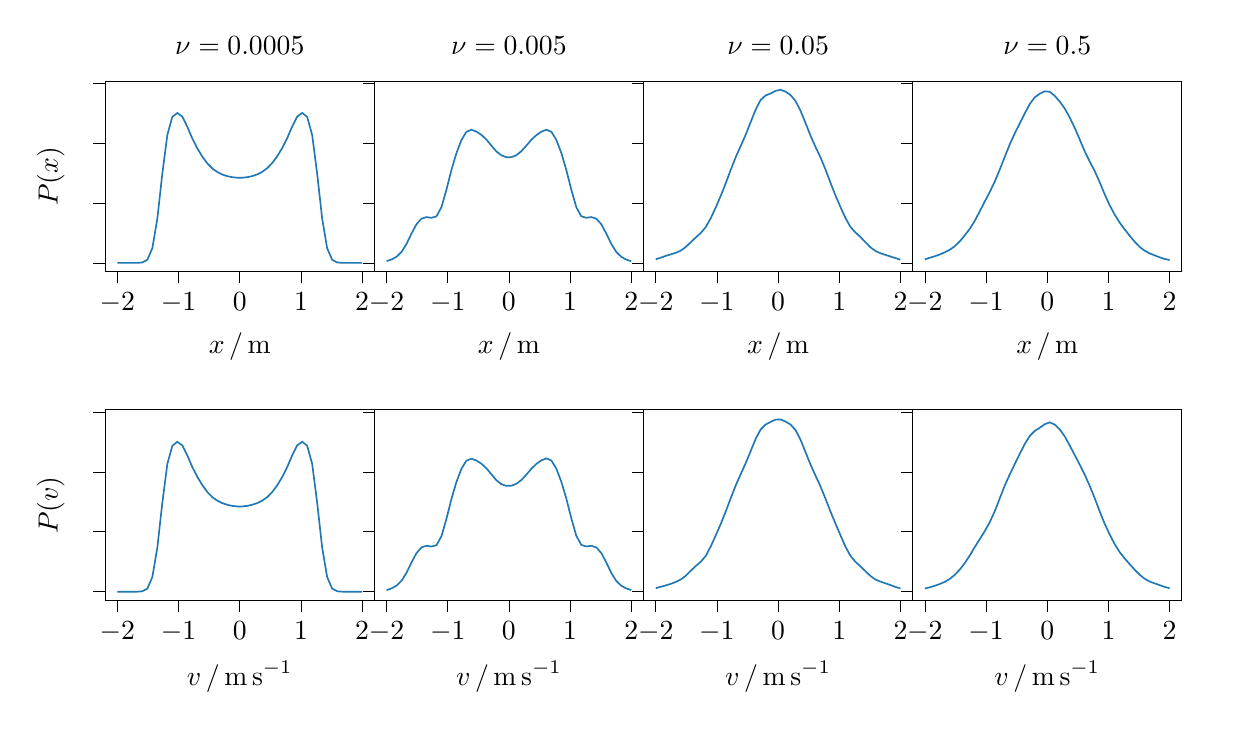
\begin{tikzpicture}

\definecolor{darkgray176}{RGB}{176,176,176}
\definecolor{steelblue31119180}{RGB}{31,119,180}

\begin{groupplot}[group style={group size=4 by 2,horizontal sep=0pt,vertical sep=50pt,yticklabels at=edge right},height=4cm,width=5cm]
\nextgroupplot[
tick align=outside,
tick pos=left,
title={\(\displaystyle \nu = 0.0005\)},
x grid style={darkgray176},
xlabel={\(\displaystyle x\,/\,\mathrm{m}\)},
xmin=-2.2, xmax=2.2,
xtick style={color=black},
y grid style={darkgray176},
ylabel={\(\displaystyle P(x)\)},
ymin=-0.0288848492832037, ymax=0.60658183623849,
ytick style={color=black}
]
\addplot [semithick, steelblue31119180]
table {%
-2 6.11775450295717e-11
-1.91836734693878 4.70066612885493e-09
-1.83673469387755 2.24563474812511e-07
-1.75510204081633 6.68108251839583e-06
-1.6734693877551 0.000124079868556266
-1.59183673469388 0.00144349508251656
-1.51020408163265 0.0105768940401462
-1.42857142857143 0.049260992486123
-1.3469387755102 0.148279603564339
-1.26530612244898 0.298049835103302
-1.18367346938776 0.426942508586909
-1.10204081632653 0.487141832867622
-1.02040816326531 0.500277867856152
-0.938775510204082 0.487916784147066
-0.857142857142857 0.454285825554003
-0.775510204081633 0.415087126006831
-0.693877551020408 0.382216881791806
-0.612244897959184 0.354855889933952
-0.530612244897959 0.332180143662908
-0.448979591836735 0.315139855709671
-0.36734693877551 0.303194965958504
-0.285714285714286 0.294985721351712
-0.204081632653061 0.289444563771024
-0.122448979591837 0.285974940345126
-0.0408163265306123 0.284261995617878
0.0408163265306123 0.28423518192165
0.122448979591836 0.285993801831124
0.204081632653061 0.289618322270837
0.285714285714286 0.295358486949551
0.36734693877551 0.303850897673412
0.448979591836734 0.316035304201495
0.530612244897959 0.333143211109938
0.612244897959183 0.355802029059258
0.693877551020408 0.383164356731793
0.775510204081633 0.416011136995191
0.857142857142857 0.455012032214682
0.938775510204081 0.488340999869285
1.02040816326531 0.500492212532273
1.10204081632653 0.487183464605509
1.18367346938775 0.426793966458542
1.26530612244898 0.29783179184179
1.3469387755102 0.148136932603607
1.42857142857143 0.0492087889083442
1.51020408163265 0.0105655253000722
1.59183673469388 0.00144198364323881
1.6734693877551 0.000123955704248286
1.75510204081633 6.67474003848864e-06
1.83673469387755 2.24361340502048e-07
1.91836734693878 4.69663990614777e-09
2 6.11273849684347e-11
};

\nextgroupplot[
scaled y ticks=manual:{}{\pgfmathparse{#1}},
tick align=outside,
tick pos=left,
title={\(\displaystyle \nu = 0.005\)},
x grid style={darkgray176},
xlabel={\(\displaystyle x\,/\,\mathrm{m}\)},
xmin=-2.2, xmax=2.2,
xtick style={color=black},
y grid style={darkgray176},
ymin=-0.0288848492832037, ymax=0.60658183623849,
ytick style={color=black},
yticklabels={}
]
\addplot [semithick, steelblue31119180]
table {%
-2 0.0058143851647466
-1.91836734693878 0.0113413918819546
-1.83673469387755 0.0205360344533247
-1.75510204081633 0.0366224772792197
-1.6734693877551 0.0634540503508966
-1.59183673469388 0.098141127362255
-1.51020408163265 0.12916458910757
-1.42857142857143 0.147646461534807
-1.3469387755102 0.152862134213635
-1.26530612244898 0.150405533137588
-1.18367346938776 0.155322784490766
-1.10204081632653 0.186287402626523
-1.02040816326531 0.244860949484816
-0.938775510204082 0.310747748195973
-0.857142857142857 0.366854149282772
-0.775510204081633 0.410497821748874
-0.693877551020408 0.437489928855338
-0.612244897959184 0.444229950824344
-0.530612244897959 0.43808550939311
-0.448979591836735 0.427020865280856
-0.36734693877551 0.411392197189834
-0.285714285714286 0.391147867344857
-0.204081632653061 0.3718465301318
-0.122448979591837 0.358831975813425
-0.0408163265306123 0.352729490138753
0.0408163265306123 0.352805530860583
0.122448979591836 0.359349360962621
0.204081632653061 0.372767057136335
0.285714285714286 0.391626563063652
0.36734693877551 0.411047055896099
0.448979591836734 0.426356679810055
0.530612244897959 0.43767845539226
0.612244897959183 0.444237271507783
0.693877551020408 0.437615670916896
0.775510204081633 0.410369396159934
0.857142857142857 0.366331594214071
0.938775510204081 0.309863549708622
1.02040816326531 0.243848643581878
1.10204081632653 0.185649587455602
1.18367346938775 0.155316366664118
1.26530612244898 0.150603753891591
1.3469387755102 0.152882147752401
1.42857142857143 0.14756901426714
1.51020408163265 0.129045937184189
1.59183673469388 0.0980412968236783
1.6734693877551 0.0634599589490442
1.75510204081633 0.0365785458974304
1.83673469387755 0.0202826275031532
1.91836734693878 0.0109701377541459
2 0.00550318633707327
};

\nextgroupplot[
scaled y ticks=manual:{}{\pgfmathparse{#1}},
tick align=outside,
tick pos=left,
title={\(\displaystyle \nu = 0.05\)},
x grid style={darkgray176},
xlabel={\(\displaystyle x\,/\,\mathrm{m}\)},
xmin=-2.2, xmax=2.2,
xtick style={color=black},
y grid style={darkgray176},
ymin=-0.0288848492832037, ymax=0.60658183623849,
ytick style={color=black},
yticklabels={}
]
\addplot [semithick, steelblue31119180]
table {%
-2 0.0118064634310015
-1.91836734693878 0.0174340513744936
-1.83673469387755 0.0232130613663361
-1.75510204081633 0.0284960057779477
-1.6734693877551 0.0335112152789481
-1.59183673469388 0.0406804886994124
-1.51020408163265 0.0528175660965527
-1.42857142857143 0.0687385333643094
-1.3469387755102 0.084639625753916
-1.26530612244898 0.0995115959377911
-1.18367346938776 0.119088386940006
-1.10204081632653 0.148498628365461
-1.02040816326531 0.18418574935171
-0.938775510204082 0.222806893719895
-0.857142857142857 0.265098538520558
-0.775510204081633 0.309677018788382
-0.693877551020408 0.351998439637468
-0.612244897959184 0.389490951236161
-0.530612244897959 0.42720422101869
-0.448979591836735 0.469274616985082
-0.36734693877551 0.511202797840088
-0.285714285714286 0.543682801176091
-0.204081632653061 0.558630679676709
-0.122448979591837 0.565183703365105
-0.0408163265306123 0.574031875579155
0.0408163265306123 0.577696986896595
0.122448979591836 0.57141892599766
0.204081632653061 0.56005115561198
0.285714285714286 0.539983286444197
0.36734693877551 0.507365069553471
0.448979591836734 0.466781399821781
0.530612244897959 0.424336744862625
0.612244897959183 0.386728954532642
0.693877551020408 0.351586140188729
0.775510204081633 0.311515945411037
0.857142857142857 0.267030809264349
0.938775510204081 0.224736832321779
1.02040816326531 0.186151688498683
1.10204081632653 0.149504826822563
1.18367346938775 0.119889554701488
1.26530612244898 0.101400060015833
1.3469387755102 0.0863723014638925
1.42857142857143 0.0688007289634417
1.51020408163265 0.0520091054119528
1.59183673469388 0.039797080378181
1.6734693877551 0.0322139604425845
1.75510204081633 0.0266728852439479
1.83673469387755 0.0214572284646834
1.91836734693878 0.0159362078200703
2 0.0107987692286987
};

\nextgroupplot[
scaled y ticks=manual:{}{\pgfmathparse{#1}},
tick align=outside,
tick pos=left,
title={\(\displaystyle \nu = 0.5\)},
x grid style={darkgray176},
xlabel={\(\displaystyle x\,/\,\mathrm{m}\)},
xmin=-2.2, xmax=2.2,
xtick style={color=black},
y grid style={darkgray176},
ymin=-0.0288848492832037, ymax=0.60658183623849,
ytick style={color=black},
yticklabels={}
]
\addplot [semithick, steelblue31119180]
table {%
-2 0.0119718140653906
-1.91836734693878 0.0172033809966442
-1.83673469387755 0.0223144202675052
-1.75510204081633 0.0281955711862652
-1.6734693877551 0.0355279224422913
-1.59183673469388 0.0441015423062132
-1.51020408163265 0.0557754292062578
-1.42857142857143 0.0722666598505082
-1.3469387755102 0.092122617877488
-1.26530612244898 0.114116487835797
-1.18367346938776 0.140885967716007
-1.10204081632653 0.172755799296933
-1.02040816326531 0.205190724576517
-0.938775510204082 0.236936472172241
-0.857142857142857 0.271922612310315
-0.775510204081633 0.311793910899495
-0.693877551020408 0.354248280862157
-0.612244897959184 0.395700845307824
-0.530612244897959 0.432571527274349
-0.448979591836735 0.465605441085597
-0.36734693877551 0.498775747310658
-0.285714285714286 0.530400990468793
-0.204081632653061 0.552429534378658
-0.122448979591837 0.564699414080358
-0.0408163265306123 0.572591028501527
0.0408163265306123 0.570857133198132
0.122448979591836 0.557323852923112
0.204081632653061 0.538431464980367
0.285714285714286 0.515073941065277
0.36734693877551 0.485240331861086
0.448979591836734 0.4505656700152
0.530612244897959 0.411890695701982
0.612244897959183 0.372426756828738
0.693877551020408 0.338295415109696
0.775510204081633 0.306511585167341
0.857142857142857 0.269399263025346
0.938775510204081 0.228906449316998
1.02040816326531 0.192254133112313
1.10204081632653 0.161050141182112
1.18367346938775 0.134546062801566
1.26530612244898 0.111845175201673
1.3469387755102 0.0907991355390343
1.42857142857143 0.0707316697918318
1.51020408163265 0.0533983431019971
1.59183673469388 0.0406904293886049
1.6734693877551 0.0319493432582222
1.75510204081633 0.0250500475622281
1.83673469387755 0.0186770696427034
1.91836734693878 0.0132138974519563
2 0.00945750512532519
};

\nextgroupplot[
tick align=outside,
tick pos=left,
x grid style={darkgray176},
xlabel={\(\displaystyle v\,/\,\mathrm{m\, s^{-1}}\)},
xmin=-2.2, xmax=2.2,
xtick style={color=black},
y grid style={darkgray176},
ylabel={\(\displaystyle P(v)\)},
ymin=-0.0288848492832037, ymax=0.60658183623849,
ytick style={color=black}
]
\addplot [semithick, steelblue31119180]
table {%
-2 5.86914524023381e-11
-1.91836734693878 4.53714669881298e-09
-1.83673469387755 2.17975825012644e-07
-1.75510204081633 6.51877558149514e-06
-1.6734693877551 0.000121639147326901
-1.59183673469388 0.00142115441672483
-1.51020408163265 0.010452891976031
-1.42857142857143 0.0488458449402282
-1.3469387755102 0.147447040871813
-1.26530612244898 0.297054319549894
-1.18367346938776 0.426219091205434
-1.10204081632653 0.486794000053463
-1.02040816326531 0.500209911265777
-0.938775510204082 0.488162909815839
-0.857142857142857 0.454918222134453
-0.775510204081633 0.416054145092474
-0.693877551020408 0.383304709933391
-0.612244897959184 0.35574682922472
-0.530612244897959 0.332731144596436
-0.448979591836735 0.315580566935527
-0.36734693877551 0.303747770308699
-0.285714285714286 0.295592555963097
-0.204081632653061 0.290013130703891
-0.122448979591837 0.286437413176055
-0.0408163265306123 0.284555851450018
0.0408163265306123 0.284465672106043
0.122448979591836 0.286371986575893
0.204081632653061 0.290143562864774
0.285714285714286 0.295729144830354
0.36734693877551 0.303797261200101
0.448979591836734 0.31557742044405
0.530612244897959 0.332427629607534
0.612244897959183 0.354981305821709
0.693877551020408 0.38242703550779
0.775510204081633 0.41547573795405
0.857142857142857 0.454697272762385
0.938775510204081 0.488195874168117
1.02040816326531 0.500456662171049
1.10204081632653 0.487214400121966
1.18367346938775 0.426680750142304
1.26530612244898 0.297399679422197
1.3469387755102 0.147620808780801
1.42857142857143 0.0489033684815528
1.51020408163265 0.0104651860506388
1.59183673469388 0.00142282568102608
1.6734693877551 0.000121781984444609
1.75510204081633 6.52638387109464e-06
1.83673469387755 2.18226823090709e-07
1.91836734693878 4.54225319907562e-09
2 5.87553324608365e-11
};

\nextgroupplot[
scaled y ticks=manual:{}{\pgfmathparse{#1}},
tick align=outside,
tick pos=left,
x grid style={darkgray176},
xlabel={\(\displaystyle v\,/\,\mathrm{m\, s^{-1}}\)},
xmin=-2.2, xmax=2.2,
xtick style={color=black},
y grid style={darkgray176},
ymin=-0.0288848492832037, ymax=0.60658183623849,
ytick style={color=black},
yticklabels={}
]
\addplot [semithick, steelblue31119180]
table {%
-2 0.00551714739605367
-1.91836734693878 0.0110421749030161
-1.83673469387755 0.0203293169073477
-1.75510204081633 0.036442341693434
-1.6734693877551 0.0632049941919938
-1.59183673469388 0.0978963905949751
-1.51020408163265 0.129119789656481
-1.42857142857143 0.147850648471358
-1.3469387755102 0.153252692209117
-1.26530612244898 0.150801679105277
-1.18367346938776 0.155215412475142
-1.10204081632653 0.185462319203967
-1.02040816326531 0.243826086669345
-0.938775510204082 0.309981710593249
-0.857142857142857 0.366467232180845
-0.775510204081633 0.410428252424829
-0.693877551020408 0.437384468033677
-0.612244897959184 0.443816578474338
-0.530612244897959 0.437728255555724
-0.448979591836735 0.427124112379046
-0.36734693877551 0.411831002348732
-0.285714285714286 0.391479968925266
-0.204081632653061 0.371716035007309
-0.122448979591837 0.35858691149742
-0.0408163265306123 0.353101497859893
0.0408163265306123 0.353823478944731
0.122448979591836 0.36018388369387
0.204081632653061 0.372647403051785
0.285714285714286 0.390735177454602
0.36734693877551 0.410336606461049
0.448979591836734 0.426485753052467
0.530612244897959 0.438404623537877
0.612244897959183 0.444868996113933
0.693877551020408 0.437829364683439
0.775510204081633 0.410444349591425
0.857142857142857 0.366706995189955
0.938775510204081 0.310632605477749
1.02040816326531 0.244735502538705
1.10204081632653 0.186489395584589
1.18367346938775 0.156058550955205
1.26530612244898 0.15110650097618
1.3469387755102 0.153183894404026
1.42857142857143 0.147801532303679
1.51020408163265 0.129067044245367
1.59183673469388 0.0975998207861607
1.6734693877551 0.0626727639078765
1.75510204081633 0.035855349623176
1.83673469387755 0.0198696150676399
1.91836734693878 0.0108244844982867
2 0.00546717718855678
};

\nextgroupplot[
scaled y ticks=manual:{}{\pgfmathparse{#1}},
tick align=outside,
tick pos=left,
x grid style={darkgray176},
xlabel={\(\displaystyle v\,/\,\mathrm{m\, s^{-1}}\)},
xmin=-2.2, xmax=2.2,
xtick style={color=black},
y grid style={darkgray176},
ymin=-0.0288848492832037, ymax=0.60658183623849,
ytick style={color=black},
yticklabels={}
]
\addplot [semithick, steelblue31119180]
table {%
-2 0.011614956824997
-1.91836734693878 0.0163548489773017
-1.83673469387755 0.0209219688614205
-1.75510204081633 0.0261441896049662
-1.6734693877551 0.0325186112816037
-1.59183673469388 0.0405875407816977
-1.51020408163265 0.0529862712735497
-1.42857142857143 0.0695283320619505
-1.3469387755102 0.08549036176856
-1.26530612244898 0.0995329214424592
-1.18367346938776 0.119216404719595
-1.10204081632653 0.150335075156849
-1.02040816326531 0.187152607863327
-0.938775510204082 0.225166899902218
-0.857142857142857 0.266852426559231
-0.775510204081633 0.311314691049764
-0.693877551020408 0.353833486170166
-0.612244897959184 0.391891877758582
-0.530612244897959 0.428473076480132
-0.448979591836735 0.468691169035506
-0.36734693877551 0.509588586154379
-0.285714285714286 0.541117230207448
-0.204081632653061 0.557719949491352
-0.122448979591837 0.566688404683057
-0.0408163265306123 0.574161704854439
0.0408163265306123 0.574798943541143
0.122448979591836 0.567808429187662
0.204081632653061 0.557700271451346
0.285714285714286 0.539238092517103
0.36734693877551 0.506927316610253
0.448979591836734 0.465533891174024
0.530612244897959 0.423919785295491
0.612244897959183 0.387269330638758
0.693877551020408 0.351007879266921
0.775510204081633 0.310172224730743
0.857142857142857 0.267345228577535
0.938775510204081 0.226943188271818
1.02040816326531 0.188034653549296
1.10204081632653 0.150047436521472
1.18367346938775 0.119440703892863
1.26530612244898 0.0997316272414308
1.3469387755102 0.0844100245611192
1.42857142857143 0.0682002023324855
1.51020408163265 0.0524604768400898
1.59183673469388 0.0406015497264836
1.6734693877551 0.0335648806260605
1.75510204081633 0.0281057447577706
1.83673469387755 0.0221498650703646
1.91836734693878 0.0160582487747666
2 0.0109877090528637
};

\nextgroupplot[
scaled y ticks=manual:{}{\pgfmathparse{#1}},
tick align=outside,
tick pos=left,
x grid style={darkgray176},
xlabel={\(\displaystyle v\,/\,\mathrm{m\, s^{-1}}\)},
xmin=-2.2, xmax=2.2,
xtick style={color=black},
y grid style={darkgray176},
ymin=-0.0288848492832037, ymax=0.60658183623849,
ytick style={color=black},
yticklabels={}
]
\addplot [semithick, steelblue31119180]
table {%
-2 0.0105873308728834
-1.91836734693878 0.0147351498615252
-1.83673469387755 0.0198949115476638
-1.75510204081633 0.0259065990005047
-1.6734693877551 0.0330573892940091
-1.59183673469388 0.0427557828852562
-1.51020408163265 0.056641053852346
-1.42857142857143 0.0742714279770395
-1.3469387755102 0.0955571009908887
-1.26530612244898 0.121414696359349
-1.18367346938776 0.149248943146021
-1.10204081632653 0.175645560718672
-1.02040816326531 0.202508594621693
-0.938775510204082 0.232480914400855
-0.857142857142857 0.268618121729021
-0.775510204081633 0.311914393246962
-0.693877551020408 0.354444740856914
-0.612244897959184 0.391462450077331
-0.530612244897959 0.426231740191707
-0.448979591836735 0.46031783470532
-0.36734693877551 0.49280618914811
-0.285714285714286 0.519970126897522
-0.204081632653061 0.536551521291684
-0.122448979591837 0.54695397274705
-0.0408163265306123 0.55891793606677
0.0408163265306123 0.565016660950064
0.122448979591836 0.557588138302581
0.204081632653061 0.541617263467511
0.285714285714286 0.518310035078635
0.36734693877551 0.48783293631112
0.448979591836734 0.455913736666006
0.530612244897959 0.424311258138328
0.612244897959183 0.390505639780525
0.693877551020408 0.353447755818725
0.775510204081633 0.312168336434773
0.857142857142857 0.26806344810678
0.938775510204081 0.226895285592817
1.02040816326531 0.190968071087271
1.10204081632653 0.158865401004489
1.18367346938775 0.132053939576313
1.26530612244898 0.11108908250438
1.3469387755102 0.0919647891323109
1.42857142857143 0.0732825127853657
1.51020408163265 0.0567006179564101
1.59183673469388 0.043325862114011
1.6734693877551 0.0340354627311093
1.75510204081633 0.0278232310250329
1.83673469387755 0.0219848643565427
1.91836734693878 0.0160322331036919
2 0.0115041129586745
};
\end{groupplot}

\end{tikzpicture}

        \caption{Distributions of displacements and velocities of a harmonic oscillator with Andersen thermostats of different \(\nu\).}
    \end{figure}

    \begin{figure}[ht!]
        \centering
        % This file was created with tikzplotlib v0.10.1.
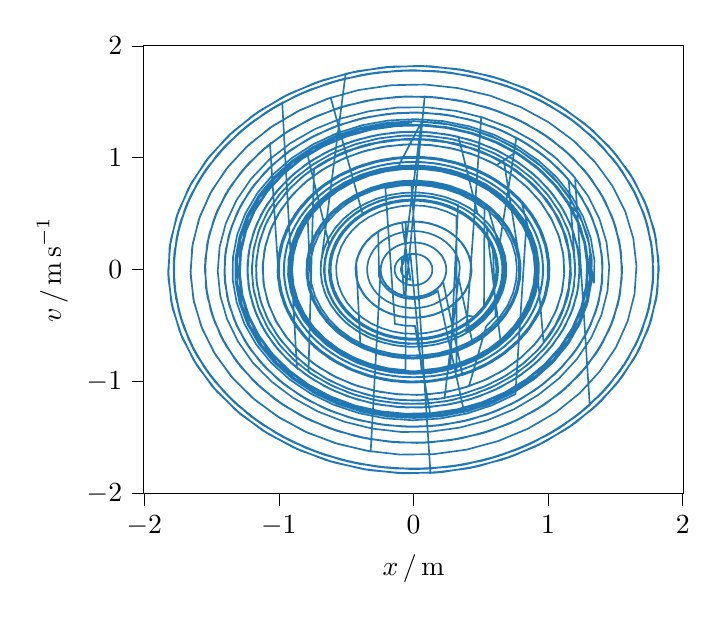
\begin{tikzpicture}

\definecolor{darkgray176}{RGB}{176,176,176}
\definecolor{steelblue31119180}{RGB}{31,119,180}

\begin{axis}[
tick align=outside,
tick pos=left,
x grid style={darkgray176},
xlabel={\(\displaystyle x\,/\,\mathrm{m}\)},
xmin=-2.0042, xmax=2.0042,
xtick style={color=black},
y grid style={darkgray176},
ylabel={\(\displaystyle v\,/\,\mathrm{m\, s^{-1}}\)},
ymin=-2.0031, ymax=2.0031,
ytick style={color=black}
]
\addplot [semithick, steelblue31119180]
table {%
0 1
0.15 0.989
0.296 0.955
0.435 0.9
0.565 0.825
0.682 0.732
0.784 0.622
0.868 0.497
0.932 0.362
0.976 0.219
0.998 0.071
0.997 -0.079
0.974 -0.227
0.929 -0.37
0.863 -0.505
0.778 -0.628
0.675 -0.738
0.558 -0.83
0.427 -0.904
0.287 -0.958
0.141 -0.99
-0.009 -1
-0.158 -0.987
-0.304 -0.953
-0.443 -0.897
-0.572 -0.82
-0.688 -0.726
-0.789 -0.615
-0.872 -0.49
-0.936 -0.354
-0.978 -0.21
-0.998 -0.062
-0.996 0.088
-0.972 0.236
-0.926 0.378
-0.859 0.513
-0.773 0.635
-0.669 0.743
-0.55 0.835
-0.419 0.908
-0.279 0.96
-0.132 0.991
0.017 1
0.167 0.986
0.312 0.95
0.451 0.893
0.579 0.815
0.695 0.72
0.794 0.608
0.876 0.482
0.939 0.346
0.98 0.202
0.999 0.053
0.996 -0.097
0.97 -0.244
0.923 -0.387
0.854 -0.52
0.767 -0.642
0.662 -0.749
0.543 -0.84
0.411 -0.912
0.271 -0.963
0.124 -0.992
-0.026 -1
-0.175 -0.985
-0.321 -0.947
-0.459 -0.889
-0.586 -0.81
-0.701 -0.714
-0.8 -0.601
-0.88 -0.475
-0.942 -0.338
-0.981 -0.193
-0.999 -0.044
-0.995 0.105
-0.968 0.253
-0.919 0.395
-0.85 0.527
-0.761 0.649
-0.656 0.755
-0.536 0.845
-0.403 0.915
-0.262 0.965
-0.115 0.993
0.035 0.999
0.184 0.983
0.329 0.944
0.466 0.885
0.593 0.805
0.707 0.707
0.805 0.594
0.885 0.214
0.907 0.079
0.908 -0.057
0.89 -0.192
0.851 -0.323
0.793 -0.446
0.717 -0.56
0.626 -0.661
0.52 -0.747
0.402 -0.816
0.276 -0.867
0.143 -0.899
0.007 -0.91
-0.129 -0.901
-0.262 -0.871
-0.389 -0.822
-0.508 -0.755
-0.615 -0.671
-0.708 -0.571
-0.786 -0.459
-0.846 -0.336
-0.886 -0.206
-0.907 -0.071
-0.908 0.065
-0.888 0.2
-0.848 0.33
-0.789 0.453
-0.713 0.566
-0.62 0.666
-0.513 0.751
-0.395 0.82
-0.268 0.869
-0.135 0.9
0.001 0.91
0.137 0.899
0.27 0.869
0.397 0.819
0.515 0.75
0.621 0.665
0.713 0.565
0.79 0.452
0.849 0.329
0.888 0.198
0.908 0.063
0.907 -0.073
0.886 -0.208
0.845 -0.338
0.785 -0.46
0.708 -0.572
0.614 -0.672
0.507 -0.756
0.388 -0.823
0.261 -0.872
0.127 -0.901
-0.009 -0.91
-0.145 -0.898
-0.277 -0.867
-0.404 -0.815
-0.521 -0.746
-0.627 -0.66
-0.718 -0.559
-0.794 -0.445
-0.851 -0.321
-0.89 -0.191
-0.908 -0.056
-0.907 0.081
-0.884 0.215
-0.842 0.345
-0.781 0.467
-0.703 0.578
-0.608 0.677
-0.5 0.76
-0.381 0.826
-0.253 0.874
-0.12 0.902
0.017 0.91
0.152 0.897
0.285 0.864
0.411 0.812
0.528 0.741
0.632 0.654
0.723 0.552
0.798 0.438
0.854 0.314
0.892 0.183
0.909 0.048
0.906 -0.089
0.882 -0.223
0.839 -0.352
0.777 -0.474
0.697 -0.585
0.602 -0.682
0.493 -0.764
0.374 -0.83
0.245 -0.876
0.112 -0.903
-0.025 -0.909
-0.16 -0.896
-0.292 -0.862
-0.418 -0.808
-0.534 -0.737
-0.638 -0.649
-0.728 -0.546
-0.801 -0.431
-0.857 -0.307
-0.893 -0.175
-0.909 -0.04
-0.905 0.097
-0.88 0.231
-0.836 0.36
-0.773 0.481
-0.692 0.591
-0.596 0.687
-0.487 0.769
-0.366 0.833
-0.238 0.878
-0.104 0.904
0.033 0.909
0.168 0.894
0.3 0.859
0.425 0.805
0.54 0.732
0.644 0.643
0.733 0.54
0.805 0.424
0.86 0.299
0.895 0.167
0.91 0.032
0.904 -0.105
0.878 -0.238
0.833 -0.367
0.769 -0.487
0.687 -0.597
0.59 -0.693
0.48 -0.773
0.359 -0.836
0.23 -0.88
0.096 -0.905
-0.04 -0.909
-0.176 -0.893
-0.307 -0.856
-0.432 -0.801
-0.547 -0.727
-0.649 -0.637
-0.737 -0.533
-0.809 -0.417
-0.862 -0.292
-0.896 -0.159
-0.91 -0.024
-0.903 0.112
-0.876 0.246
-0.83 0.374
-0.764 0.494
-0.682 0.603
-0.584 0.698
-0.473 0.777
-0.352 0.839
-0.222 0.882
-0.088 0.906
0.048 0.909
0.184 0.891
0.315 0.854
0.439 0.797
0.553 0.722
0.655 0.632
0.742 0.527
0.812 0.41
0.865 0.284
0.897 0.152
0.91 0.016
0.902 -0.12
0.874 -0.254
0.826 -0.381
0.76 -0.501
0.677 -0.609
0.578 -0.703
0.466 -0.781
0.344 -0.842
0.215 -0.884
0.08 -0.906
-0.056 -0.908
-0.191 -0.889
-0.322 -0.851
-0.446 -0.793
-0.559 -0.718
-0.66 -0.626
-0.747 -0.52
-0.816 -0.403
-0.867 -0.276
-0.899 -0.144
-0.91 -0.008
-0.901 0.128
-0.872 0.261
-0.823 0.389
-0.756 0.507
-0.671 0.614
-0.572 0.708
-0.46 0.785
-0.337 0.845
-0.207 0.886
-0.072 0.907
0.064 0.908
0.199 0.888
0.33 0.848
0.453 0.789
0.566 0.713
0.666 0.62
0.751 0.514
0.82 0.396
0.869 0.269
0.9 0.136
0.91 -0
0.9 -0.136
0.869 -0.269
0.819 -0.396
0.751 -0.514
0.666 -0.62
0.566 -0.713
0.453 -0.789
0.33 -0.848
0.199 -0.888
0.064 -0.908
-0.072 -0.907
-0.207 -0.886
-0.337 -0.845
-0.46 -0.785
-0.572 -0.708
-0.671 -0.614
-0.756 -0.507
-0.823 -0.389
-0.872 -0.261
-0.901 -0.128
-0.91 0.008
-0.899 0.144
-0.867 0.277
-0.816 0.403
-0.747 0.52
-0.66 0.626
-0.559 0.718
-0.446 0.793
-0.322 0.851
-0.191 0.889
-0.056 0.908
0.08 0.906
0.215 0.884
0.344 0.842
0.467 0.781
0.578 0.703
0.677 0.608
0.76 0.501
0.826 0.381
0.874 0.254
0.902 0.12
0.91 -0.016
0.897 -0.152
0.865 -0.284
0.812 -0.41
0.742 -0.527
0.655 -0.632
0.553 -0.723
0.439 -0.797
0.315 -0.854
0.184 -0.891
0.048 -0.909
-0.088 -0.906
-0.222 -0.882
-0.352 -0.839
-0.473 -0.777
-0.584 -0.698
-0.682 -0.603
-0.764 -0.494
-0.83 -0.374
-0.876 -0.246
-0.903 -0.112
-0.91 0.024
-0.896 0.16
-0.862 0.292
-0.809 0.417
-0.737 0.533
-0.649 0.637
-0.547 0.727
-0.432 0.801
-0.307 0.856
-0.176 0.893
-0.04 0.909
0.096 0.905
0.23 0.88
0.359 0.836
0.48 0.773
0.59 0.693
0.687 0.597
0.769 0.487
0.833 0.367
0.878 0.238
0.904 0.104
0.91 -0.032
0.895 -0.167
0.86 -0.299
0.805 -0.424
0.733 -0.54
0.644 -0.643
0.54 -0.732
0.425 -0.805
0.3 -0.859
0.168 -0.894
0.032 -0.909
-0.104 -0.904
-0.238 -0.878
-0.366 -0.833
-0.487 -0.769
-0.596 -0.687
-0.692 -0.591
-0.773 -0.48
-0.836 -0.36
-0.88 -0.231
-0.905 -0.097
-0.909 0.04
-0.893 0.175
-0.857 0.307
-0.801 0.431
-0.728 0.546
-0.638 0.649
-0.534 0.737
-0.418 0.808
-0.292 0.862
-0.16 0.896
-0.024 0.909
0.112 0.903
0.245 0.876
0.374 0.83
0.494 0.764
0.602 0.682
0.697 0.584
0.777 0.474
0.839 0.352
0.882 0.223
0.906 0.089
0.909 -0.048
0.892 -0.183
0.854 -0.314
0.798 -0.438
0.723 -0.552
0.632 -0.654
0.527 -0.741
0.411 -0.812
0.285 -0.864
0.152 -0.897
0.017 -0.91
-0.12 -0.902
-0.253 -0.874
-0.381 -0.826
-0.5 -0.76
-0.608 -0.677
-0.703 -0.578
-0.781 -0.467
-0.842 -0.345
-0.884 -0.215
-0.907 -0.081
-0.908 0.056
-0.89 0.191
-0.851 0.322
-0.794 0.445
-0.718 0.559
-0.627 0.66
-0.521 0.746
-0.404 0.815
-0.277 0.867
-0.145 0.898
-0.009 0.91
0.128 0.901
0.261 0.872
0.388 0.823
0.507 0.756
0.614 0.671
0.708 0.572
0.785 0.46
0.845 0.338
0.886 0.208
0.907 0.073
0.908 -0.064
0.888 -0.199
0.849 -0.329
0.79 -0.452
0.713 -0.565
0.621 -0.665
0.514 -0.751
0.396 -0.819
0.27 -0.869
0.137 -0.9
0.001 -0.91
-0.135 -0.9
-0.268 -0.869
-0.395 -0.82
-0.513 -0.751
-0.62 -0.666
-0.713 -0.566
-0.789 -0.453
-0.848 -0.33
-0.888 -0.2
-0.908 -0.065
-0.907 0.072
-0.886 0.206
-0.846 0.336
-0.786 0.459
-0.768 -0.025
-0.763 0.09
-0.741 0.203
-0.702 0.312
-0.648 0.413
-0.579 0.505
-0.497 0.586
-0.404 0.654
-0.301 0.707
-0.192 0.744
-0.079 0.764
0.036 0.768
0.151 0.753
0.262 0.722
0.367 0.675
0.464 0.613
0.55 0.537
0.624 0.449
0.684 0.35
0.729 0.244
0.757 0.133
0.768 0.018
0.762 -0.097
0.739 -0.21
0.7 -0.318
0.644 -0.419
0.574 -0.511
0.492 -0.591
0.398 -0.657
0.295 -0.709
0.186 -0.746
0.072 -0.765
-0.043 -0.767
-0.157 -0.752
-0.268 -0.72
-0.373 -0.672
-0.469 -0.609
-0.555 -0.532
-0.628 -0.443
-0.687 -0.344
-0.731 -0.238
-0.758 -0.126
-0.769 -0.011
-0.762 0.104
-0.738 0.216
-0.697 0.324
-0.641 0.425
-0.57 0.516
-0.486 0.595
-0.392 0.661
-0.289 0.712
-0.179 0.747
-0.065 0.766
0.05 0.767
0.164 0.751
0.274 0.718
0.378 0.669
0.474 0.605
0.559 0.527
0.623 0.262
0.655 0.166
0.673 0.066
0.675 -0.035
0.662 -0.136
0.634 -0.233
0.592 -0.325
0.537 -0.41
0.47 -0.486
0.392 -0.55
0.503 1.364
0.701 1.274
0.883 1.155
1.046 1.01
1.185 0.842
1.298 0.655
1.381 0.454
1.434 0.243
1.454 0.026
1.441 -0.192
1.396 -0.405
1.32 -0.609
1.214 -0.799
1.081 -0.972
0.924 -1.122
0.746 -1.248
0.551 -1.345
0.343 -1.412
0.128 -1.448
-0.09 -1.451
-0.305 -1.421
-0.514 -1.359
-0.712 -1.267
-0.893 -1.147
-1.055 -1
-1.193 -0.832
-1.303 -0.644
-1.385 -0.442
-1.436 -0.23
-1.454 -0.013
-1.44 0.204
-1.393 0.417
-1.315 0.62
-1.207 0.81
-1.073 0.981
-0.914 1.13
-0.735 1.254
-0.539 1.35
-0.331 1.415
-0.116 1.449
0.102 1.45
0.318 1.418
0.526 1.355
0.723 1.261
0.903 1.139
1.063 0.991
1.2 0.821
1.309 -1.21
1.113 -1.392
0.893 -1.542
0.652 -1.658
0.397 -1.737
0.133 -1.777
-0.134 -1.777
-0.398 -1.737
-0.654 -1.658
-0.894 -1.542
-1.114 -1.391
-1.31 -1.209
-1.476 -0.999
-1.609 -0.768
-1.705 -0.519
-1.764 -0.258
-1.782 0.008
-1.761 0.275
-1.7 0.535
-1.601 0.783
-1.466 1.013
-1.298 1.221
-1.101 1.401
-0.879 1.55
-0.638 1.664
-0.382 1.741
-0.117 1.778
0.15 1.776
0.414 1.733
0.668 1.652
0.907 1.534
1.127 1.381
1.32 1.197
1.485 0.986
1.615 0.753
1.71 0.504
1.766 0.243
1.782 -0.024
1.759 -0.29
1.696 -0.55
1.594 -0.797
1.457 -1.026
1.288 -1.232
1.089 -1.411
0.866 -1.558
0.623 -1.669
0.367 -1.744
0.102 -1.779
-0.165 -1.774
-0.429 -1.73
-0.682 -1.646
-0.921 -1.526
-1.139 -1.371
-1.331 -1.186
-1.493 -0.973
-1.622 -0.739
-1.714 -0.489
-1.768 -0.227
-1.782 0.04
-1.756 0.305
-1.691 0.564
-1.587 0.811
-1.448 1.039
-1.277 1.243
-1.077 1.42
-0.852 1.565
-0.609 1.675
-0.351 1.747
-0.086 1.78
0.181 1.773
0.444 1.726
0.697 1.64
0.934 1.518
1.151 1.361
1.341 1.174
1.502 0.96
1.628 0.725
1.718 0.474
1.77 0.212
1.782 -0.055
1.753 -0.321
1.686 -0.579
1.58 -0.824
1.439 -1.051
1.266 -1.254
1.064 -1.43
0.839 -1.572
0.594 -1.68
0.336 -1.75
0.071 -1.781
-0.196 -1.771
-0.459 -1.722
-0.711 -1.634
-0.947 -1.509
-1.162 -1.351
-1.351 -1.162
-1.51 -0.947
-1.635 -0.711
-1.722 -0.459
-1.772 -0.196
-1.781 0.071
-1.751 0.336
-1.681 0.594
-1.573 0.838
-1.43 1.064
-1.255 1.266
-1.052 1.439
-0.825 1.58
-0.579 1.685
-0.321 1.753
-0.055 1.781
0.212 1.769
0.474 1.718
0.725 1.628
0.961 1.501
1.174 1.341
1.361 1.15
1.518 0.934
1.641 0.697
1.726 0.444
1.773 0.181
1.78 -0.086
1.748 -0.351
1.675 -0.608
1.566 -0.852
1.421 -1.076
1.244 -1.276
1.039 -1.448
0.811 -1.587
0.565 -1.69
0.306 -1.756
0.04 -1.782
-0.227 -1.767
-0.489 -1.714
-0.74 -1.621
-0.974 -1.493
-1.186 -1.33
-1.371 -1.138
-1.526 -0.921
-1.647 -0.682
-1.73 -0.429
-1.775 -0.165
-1.78 0.102
-1.744 0.367
-1.67 0.623
-1.558 0.866
-1.411 1.089
-1.233 1.287
-1.026 1.457
-0.797 1.594
-0.55 1.695
-0.29 1.758
-0.024 1.782
0.243 1.765
0.504 1.709
0.754 1.615
0.987 1.484
1.197 1.32
1.381 1.126
1.534 0.907
1.653 0.668
1.734 0.413
1.776 0.15
1.779 -0.117
1.741 -0.382
1.665 -0.638
1.55 -0.879
1.402 -1.101
1.221 -1.298
1.014 -1.466
0.783 -1.601
0.535 -1.7
0.275 -1.761
0.008 -1.782
-0.258 -1.763
-0.519 -1.705
-0.768 -1.608
-1 -1.475
-1.209 -1.31
-1.391 -1.114
-1.542 -0.894
-1.658 -0.653
-1.737 -0.398
-1.777 -0.134
-1.778 0.133
-1.738 0.397
-1.659 0.652
-1.543 0.893
-1.392 1.113
-1.21 1.309
-1.001 1.475
-0.769 1.608
-0.52 1.704
-0.259 1.763
0.007 1.782
0.273 1.761
0.534 1.7
0.782 1.601
1.012 1.467
1.22 1.299
1.401 1.102
1.55 0.88
1.664 0.639
1.741 0.383
1.779 0.119
1.776 -0.148
1.734 -0.412
1.653 -0.667
1.535 -0.906
1.382 -1.125
1.198 -1.319
0.988 -1.483
0.755 -1.614
0.505 -1.709
0.244 -1.765
-0.023 -1.782
-0.289 -1.758
-0.548 -1.696
-0.796 -1.595
-1.025 -1.458
-1.232 -1.288
-1.41 -1.09
-1.557 -0.867
-1.67 -0.624
-1.744 -0.368
-1.78 -0.103
-1.775 0.164
-1.731 0.427
-1.647 0.681
-1.527 0.919
-1.372 1.137
-1.187 1.329
-0.975 1.492
-0.866 -0.879
-0.988 -0.739
-1.087 -0.584
-1.162 -0.415
-1.211 -0.236
-1.233 -0.053
-1.227 0.132
-1.193 0.314
-1.133 0.489
-1.047 0.652
-0.938 0.801
-0.808 0.933
-0.659 1.043
-0.496 1.13
-0.321 1.191
-0.14 1.226
0.045 1.233
0.229 1.212
0.408 1.164
0.577 1.09
0.734 0.992
0.874 0.871
0.994 0.731
1.092 0.574
1.166 0.404
1.213 0.226
1.233 0.042
1.226 -0.143
1.191 -0.324
1.129 -0.498
1.041 -0.661
0.931 -0.81
0.799 -0.94
0.65 -1.049
0.486 -1.134
0.311 -1.194
0.129 -1.227
-0.056 -1.232
-0.239 -1.21
-0.418 -1.161
-0.587 -1.085
-0.742 -0.985
-0.881 -0.863
-1 -0.722
-1.097 -0.565
-1.169 -0.394
-1.215 -0.215
-1.233 -0.031
-1.224 0.153
-1.188 0.335
-1.124 0.508
-1.036 0.671
-0.924 0.818
-0.791 0.947
-0.641 1.054
-0.476 1.138
-0.3 1.196
-0.118 1.228
0.067 1.232
0.25 1.208
0.428 1.157
0.596 1.08
0.751 0.979
0.889 0.856
1.007 0.713
1.102 0.555
1.173 0.384
1.217 0.205
1.234 0.02
1.223 -0.164
1.185 -0.345
1.12 -0.518
1.03 -0.68
0.917 -0.826
0.783 -0.953
0.632 -1.06
0.466 -1.142
0.29 -1.199
0.108 -1.229
-0.077 -1.231
-0.261 -1.206
-0.438 -1.153
-0.605 -1.075
-0.759 -0.972
-0.896 -0.848
-1.013 -0.705
-1.107 -0.545
-1.176 -0.374
-1.219 -0.194
-1.234 -0.01
-1.221 0.175
-1.182 0.355
-1.115 0.528
-1.024 0.689
-0.909 0.834
-0.774 0.96
-0.622 1.065
-0.456 1.146
-0.28 1.201
-0.097 1.23
0.088 1.23
0.271 1.203
0.448 1.149
0.615 1.07
0.768 0.966
0.903 0.84
1.019 0.696
1.111 0.536
1.179 0.364
1.22 0.183
1.234 -0.001
1.22 -0.185
1.178 -0.366
1.111 -0.538
1.018 -0.697
0.902 -0.842
0.766 -0.967
0.613 -1.071
0.446 -1.15
0.269 -1.204
0.086 -1.231
-0.099 -1.23
-0.282 -1.201
-0.458 -1.145
-0.624 -1.064
-0.776 -0.959
-0.911 -0.832
-1.025 -0.687
-1.116 -0.526
-1.182 -0.353
-1.222 -0.173
-1.234 0.012
-1.218 0.196
-1.175 0.376
-1.106 0.547
-1.012 0.706
-0.895 0.85
-0.758 0.974
-0.604 1.076
-0.436 1.154
-0.258 1.206
-0.075 1.231
0.11 1.229
0.292 1.198
0.468 1.141
0.633 1.059
0.785 0.952
0.918 0.824
1.031 0.678
1.121 0.516
1.185 0.343
1.223 0.162
1.234 -0.023
1.216 -0.207
1.172 -0.386
1.101 -0.557
1.005 -0.715
0.887 -0.857
0.749 -0.98
0.594 -1.081
0.426 -1.158
0.248 -1.208
0.064 -1.232
-0.12 -1.228
-0.303 -1.196
-0.478 -1.137
-0.643 -1.053
-0.793 -0.945
-0.925 -0.816
-1.037 -0.669
-1.125 -0.506
-1.188 -0.333
-1.225 -0.151
-1.233 0.033
-1.215 0.217
-1.168 0.396
-1.096 0.566
-0.999 0.724
-0.88 0.865
-0.74 0.987
-0.585 1.086
-0.416 1.161
-0.237 1.21
-0.054 1.232
0.131 1.227
0.313 1.193
0.488 1.133
0.652 1.047
0.801 0.938
0.932 0.808
1.043 0.66
1.13 0.496
1.191 0.322
1.226 0.141
1.233 -0.044
1.213 -0.228
1.165 -0.407
1.091 -0.576
0.993 -0.733
0.872 -0.873
0.732 -0.993
0.575 -1.091
0.405 -1.165
0.227 -1.212
0.043 -1.233
-0.142 -1.225
-0.323 -1.19
-0.498 -1.129
-0.661 -1.042
-0.809 -0.931
-0.939 -0.8
-1.048 -0.651
-1.134 -0.487
-1.194 -0.312
-1.227 -0.13
-1.233 0.055
-1.211 0.238
-1.161 0.417
-1.086 0.586
-0.986 0.741
-0.864 0.88
-0.723 0.999
-0.566 1.096
-0.395 1.168
-0.216 1.214
-0.032 1.233
0.153 1.224
0.334 1.188
0.476 0.499
0.546 0.423
0.603 0.336
0.646 0.242
0.675 0.143
0.689 0.041
0.687 -0.063
0.67 -0.165
0.638 -0.263
0.592 -0.355
0.532 -0.44
0.46 -0.514
0.378 -0.577
0.288 -0.627
0.191 -0.663
0.089 -0.684
-0.014 -0.69
-0.117 -0.68
-0.217 -0.655
-0.313 -0.615
-0.401 -0.561
-0.481 -0.495
-0.549 -0.418
-0.606 -0.331
-0.648 -0.237
-0.676 -0.137
-0.689 -0.035
-0.687 0.069
-0.669 0.17
-0.636 0.269
-0.588 0.36
-0.528 0.444
-0.456 0.518
-0.373 0.58
-0.282 0.63
-0.185 0.665
-0.083 0.685
0.02 0.69
0.123 0.679
0.223 0.653
0.318 0.612
0.406 0.558
0.485 0.491
0.553 0.413
0.608 0.326
0.65 0.231
0.678 0.131
0.69 0.029
0.686 -0.075
0.667 -0.176
0.633 -0.274
0.585 -0.366
0.524 -0.449
0.451 -0.522
0.368 -0.584
0.277 -0.632
0.179 -0.666
0.077 -0.686
-0.026 -0.689
-0.129 -0.678
-0.229 -0.651
-0.323 -0.609
-0.411 -0.554
-0.489 -0.487
-0.556 -0.408
-0.611 -0.32
-0.652 -0.225
-0.679 -0.125
-0.69 -0.023
-0.685 0.081
-0.666 0.182
-0.631 0.28
-0.582 0.371
-0.52 0.454
-0.447 0.526
-0.363 0.587
-0.271 0.635
-0.173 0.668
-0.071 0.686
0.032 0.689
0.135 0.677
0.234 0.649
0.329 0.607
0.416 0.551
0.493 0.482
0.56 0.403
0.614 0.315
0.654 0.22
0.68 0.12
0.69 0.017
0.685 -0.087
0.664 -0.188
0.629 -0.285
0.579 -0.376
0.516 -0.458
0.442 -0.53
0.358 -0.59
0.265 -0.637
0.167 -0.669
0.065 -0.687
-0.038 -0.689
-0.141 -0.675
-0.24 -0.647
-0.334 -0.604
-0.421 -0.547
-0.498 -0.478
-0.564 -0.398
-0.617 -0.31
-0.656 -0.214
-0.681 -0.114
-0.69 -0.011
-0.684 0.093
-0.662 0.194
-0.626 0.291
-0.576 0.381
-0.512 0.463
-0.437 0.534
-0.353 0.593
-0.26 0.639
-0.161 0.671
-0.059 0.687
0.044 0.689
0.147 0.674
0.246 0.645
0.339 0.601
0.425 0.543
0.502 0.474
0.567 0.393
0.619 0.304
0.658 0.208
0.682 0.108
0.69 0.005
0.683 -0.099
0.661 -0.2
0.623 -0.296
0.572 -0.386
0.508 -0.467
0.433 -0.538
0.347 -0.596
0.254 -0.641
0.156 -0.672
0.053 -0.688
-0.05 -0.688
-0.152 -0.673
-0.251 -0.643
-0.345 -0.598
-0.43 -0.54
-0.506 -0.469
-0.57 -0.388
-0.622 -0.299
-0.66 -0.203
-0.683 -0.102
-0.69 0.001
-0.682 0.105
-0.504 1.751
-0.236 1.806
0.036 1.821
0.308 1.795
0.573 1.729
0.825 1.624
1.059 1.483
1.269 1.308
1.45 1.104
1.599 0.875
1.711 0.626
1.786 0.363
1.82 0.092
1.813 -0.181
1.766 -0.449
1.679 -0.708
1.554 -0.951
1.395 -1.173
1.204 -1.368
0.986 -1.532
0.745 -1.662
0.488 -1.755
0.221 -1.808
-0.052 -1.821
-0.324 -1.793
-0.588 -1.724
-0.839 -1.617
-1.072 -1.473
-1.28 -1.297
-1.459 -1.091
-1.606 -0.861
-1.717 -0.611
-1.789 -0.348
-1.821 -0.076
-1.812 0.196
-1.762 0.465
-1.673 0.723
-1.546 0.965
-1.384 1.185
-1.192 1.378
-0.972 1.541
-0.731 1.669
-0.473 1.759
-0.205 1.81
0.068 1.82
0.34 1.79
0.603 1.719
0.853 1.61
1.085 1.464
1.291 1.285
1.469 1.078
1.614 0.847
1.722 0.596
1.792 0.332
1.821 0.061
1.81 -0.212
1.758 -0.48
1.666 -0.737
1.537 -0.978
1.374 -1.197
1.179 -1.389
0.959 -1.549
0.716 -1.675
0.458 -1.763
0.189 -1.812
-0.084 -1.82
-0.355 -1.787
-0.618 -1.714
-0.868 -1.602
-1.097 -1.454
-1.302 -1.274
-1.478 -1.065
-1.621 -0.832
-1.727 -0.581
-1.795 -0.316
-1.822 -0.045
-1.808 0.228
-1.754 0.496
-1.66 0.752
-1.529 0.992
-1.363 1.209
-1.167 1.399
-0.945 1.558
-0.702 1.681
-0.442 1.767
-0.173 1.813
0.1 1.819
0.371 1.784
0.633 1.708
0.881 1.594
1.11 1.445
1.313 1.263
1.488 1.052
1.628 0.818
1.732 0.566
1.797 0.301
1.822 0.029
1.806 -0.244
1.749 -0.511
1.653 -0.766
1.52 -1.005
1.353 -1.221
1.155 -1.409
0.931 -1.566
0.687 -1.687
0.427 -1.771
0.157 -1.815
-0.116 -1.818
-0.386 -1.78
-0.648 -1.703
-0.895 -1.587
-1.123 -1.435
-1.324 -1.251
-1.497 -1.039
-1.635 -0.804
-1.737 -0.551
-1.8 -0.285
-1.822 -0.013
-1.804 0.26
-1.745 0.526
-1.646 0.781
-1.511 1.018
-1.342 1.232
-1.143 1.419
-0.918 1.574
-0.672 1.693
-0.411 1.775
-0.141 1.816
0.132 1.817
0.402 1.777
0.663 1.697
0.909 1.579
1.135 1.425
1.335 1.24
1.506 1.026
1.642 0.79
1.742 0.535
1.802 0.269
1.822 -0.003
1.801 -0.275
1.74 -0.541
1.639 -0.795
1.502 -1.031
1.331 -1.244
1.13 -1.429
0.904 -1.582
0.657 -1.699
0.396 -1.778
0.126 -1.817
-0.017 0.786
0.1 0.78
0.216 0.756
0.326 0.715
0.43 0.658
0.523 0.587
0.605 0.502
0.673 0.406
0.727 0.301
0.763 0.189
0.783 0.073
0.785 -0.045
0.77 -0.162
0.737 -0.275
0.687 -0.382
0.623 -0.48
0.544 -0.568
0.453 -0.643
0.351 -0.703
0.242 -0.748
0.128 -0.776
0.01 -0.786
-0.107 -0.779
-0.222 -0.754
-0.333 -0.712
-0.435 -0.655
-0.528 -0.582
-0.61 -0.497
-0.677 -0.4
-0.729 -0.294
-0.765 -0.182
-0.784 -0.066
-0.785 0.052
-0.768 0.169
-0.734 0.281
-0.684 0.388
-0.618 0.486
-0.539 0.573
-0.447 0.647
-0.345 0.706
-0.236 0.75
-0.121 0.777
-0.004 0.786
0.114 0.778
0.229 0.752
0.339 0.709
0.441 0.651
0.533 0.578
0.614 0.491
0.68 0.394
0.732 0.288
0.767 0.176
0.784 0.059
0.784 -0.059
0.767 -0.175
0.732 -0.288
0.681 -0.394
0.614 -0.491
0.534 -0.577
0.441 -0.651
0.339 -0.709
0.229 -0.752
0.114 -0.778
-0.003 -0.786
-0.121 -0.777
-0.236 -0.75
-0.345 -0.706
-0.447 -0.647
-0.539 -0.573
-0.618 -0.486
-0.684 -0.388
-0.734 -0.282
-0.768 -0.169
-0.785 -0.052
-0.784 0.066
-0.765 0.182
-0.729 0.294
-0.677 0.4
-0.61 0.497
-0.529 0.582
-0.436 0.655
-0.333 0.712
-0.223 0.754
-0.107 0.779
0.01 0.786
0.128 0.776
0.242 0.748
0.351 0.703
0.452 0.643
0.544 0.568
0.622 0.481
0.687 0.382
0.737 0.275
0.77 0.162
0.785 0.045
0.783 -0.072
0.763 -0.189
0.727 -0.301
0.674 -0.406
0.605 -0.502
0.524 -0.587
0.43 -0.658
0.327 -0.715
0.216 -0.756
0.101 -0.78
-0.017 -0.786
-0.134 -0.775
-0.249 -0.746
-0.357 -0.7
-0.458 -0.639
-0.548 -0.563
-0.627 -0.475
-0.691 -0.376
-0.739 -0.269
-0.771 -0.155
-0.785 -0.038
-0.782 0.079
-0.762 0.195
-0.724 0.307
-0.67 0.412
-0.601 0.507
-0.518 0.591
-0.424 0.662
-0.32 0.718
-0.209 0.758
-0.094 0.781
0.024 0.786
0.141 0.773
0.255 0.744
0.363 0.697
0.464 0.635
0.553 0.559
0.631 0.47
0.694 0.37
0.741 0.262
0.772 0.149
0.786 0.032
0.782 -0.086
0.76 -0.202
0.721 -0.313
0.666 -0.417
0.596 -0.512
0.513 -0.596
0.418 -0.666
0.314 -0.721
0.203 -0.76
0.087 -0.781
-0.031 -0.786
-0.148 -0.772
-0.262 -0.741
-0.37 -0.694
-0.469 -0.631
-0.558 -0.554
-0.635 -0.464
-0.697 -0.364
-0.744 -0.256
-0.774 -0.142
-0.786 -0.025
-0.781 0.093
-0.758 0.209
-0.719 0.32
-0.663 0.423
-0.592 0.518
-0.508 0.6
-0.413 0.669
-0.308 0.723
-0.196 0.761
-0.08 0.782
0.038 0.785
0.155 0.771
0.268 0.739
0.376 0.691
0.475 0.627
0.563 0.549
0.639 0.459
0.7 0.358
0.746 0.249
0.775 0.135
0.786 0.018
0.78 -0.1
0.756 -0.215
0.716 -0.326
0.659 -0.429
0.587 -0.523
0.503 -0.605
0.407 -0.673
0.301 -0.726
0.19 -0.763
0.073 -0.783
-0.044 -0.785
-0.161 -0.769
-0.275 -0.737
-0.382 -0.687
-0.48 -0.623
-0.568 -0.544
-0.643 -0.453
-0.703 -0.352
-0.748 -0.243
-0.776 -0.128
-0.786 -0.011
-0.779 0.107
-0.754 0.222
-0.713 0.332
-0.655 0.435
-0.583 0.528
-0.497 0.609
-0.401 0.676
-0.295 0.729
-0.183 0.765
-0.067 0.783
0.051 0.785
0.168 0.768
0.281 0.734
0.388 0.684
0.486 0.618
0.573 0.539
0.647 0.447
0.706 0.346
0.75 0.236
0.777 0.122
0.786 0.004
0.778 -0.113
0.753 -0.228
0.71 -0.338
0.651 -0.441
0.578 -0.533
0.492 -0.613
0.395 -0.68
0.289 -0.731
0.176 -0.766
0.06 -0.784
-0.058 -0.784
-0.175 -0.767
-0.287 -0.732
-0.394 -0.681
-0.491 -0.614
-0.577 -0.534
-0.651 -0.442
-0.709 -0.34
-0.752 -0.23
-0.778 -0.115
-0.786 0.003
-0.777 0.12
-0.751 0.235
-0.707 0.344
-0.648 0.446
-0.574 0.538
-0.487 0.618
-0.389 0.683
-0.282 0.734
-0.169 0.768
-0.053 0.784
0.065 0.783
0.181 0.765
0.294 0.729
0.4 0.677
0.496 0.61
0.582 0.529
0.654 0.436
0.712 0.335
0.754 0.225
0.779 0.11
0.787 -0.008
0.777 -0.126
0.75 -0.24
0.705 -0.35
0.645 -0.451
0.57 -0.542
0.483 -0.621
0.385 -0.687
0.278 -0.736
0.164 -0.77
0.047 -0.785
-0.07 -0.784
-0.187 -0.764
-0.299 -0.728
-0.405 -0.675
-0.501 -0.607
-0.586 -0.525
-0.658 -0.432
-0.715 -0.329
-0.756 -0.218
-0.78 -0.103
-0.787 0.015
-0.776 0.132
-0.747 0.247
-0.702 0.356
-0.641 0.457
-0.566 0.547
-0.477 0.626
-0.379 0.69
-0.271 0.739
-0.158 0.771
-0.041 0.786
0.077 0.783
0.194 0.763
0.305 0.725
0.41 0.671
0.506 0.603
0.591 0.52
0.662 0.426
0.718 0.322
0.758 0.212
0.781 0.096
0.787 -0.022
0.775 -0.139
0.745 -0.253
0.699 -0.362
0.637 -0.462
0.561 -0.552
0.472 -0.63
0.372 -0.693
0.265 -0.741
0.151 -0.772
0.034 -0.786
-0.084 -0.782
-0.2 -0.761
-0.312 -0.723
-0.416 -0.668
-0.511 -0.598
-0.595 -0.515
-0.665 -0.42
-0.721 -0.316
-0.76 -0.205
-0.782 -0.089
-0.787 0.029
-0.773 0.146
-0.743 0.26
-0.696 0.368
-0.633 0.468
-0.556 0.557
-0.466 0.634
-0.366 0.696
-0.258 0.743
-0.144 0.774
-0.027 0.786
0.091 0.782
0.207 0.759
0.318 0.72
0.422 0.664
0.517 0.594
0.6 0.51
0.669 0.415
0.724 0.31
0.762 0.198
0.783 0.082
0.786 -0.036
0.772 -0.153
0.741 -0.266
0.693 -0.374
0.629 -0.473
0.551 -0.562
0.461 -0.638
0.36 -0.7
0.252 -0.746
0.137 -0.775
0.02 -0.787
-0.098 -0.781
-0.213 -0.757
-0.324 -0.717
-0.428 -0.66
-0.522 -0.589
-0.604 -0.505
-0.673 -0.409
-0.726 -0.304
-0.763 -0.192
-0.784 -0.075
-0.786 0.042
-0.771 0.159
-0.738 0.273
-0.689 0.38
-0.625 0.479
-0.546 0.567
-0.455 0.642
-0.354 0.703
-0.245 0.748
-0.131 0.776
-0.013 0.787
0.105 0.78
0.22 0.756
0.331 0.714
0.434 0.657
0.527 0.585
0.608 0.499
0.676 0.403
0.729 0.297
0.765 0.185
0.784 0.069
0.786 -0.049
0.769 -0.166
0.736 -0.279
0.686 -0.386
0.62 -0.484
0.541 -0.571
0.45 -0.646
0.348 -0.706
0.239 -0.75
0.124 -0.777
0.006 -0.787
-0.111 -0.779
-0.227 -0.754
-0.337 -0.711
-0.439 -0.653
-0.532 -0.58
-0.613 -0.494
-0.68 -0.397
-0.731 -0.291
-0.767 -0.178
-0.785 -0.062
-0.785 0.056
-0.768 0.173
-0.733 0.286
-0.682 0.392
-0.616 0.49
-0.536 0.576
-0.444 0.65
-0.342 0.709
-0.232 0.752
-0.117 0.778
0.001 0.787
0.118 0.778
0.233 0.752
0.343 0.708
0.445 0.649
0.537 0.575
0.617 0.489
0.683 0.391
0.734 0.284
0.768 0.172
0.785 0.055
0.785 -0.063
0.766 -0.18
0.731 -0.292
0.679 -0.398
0.612 -0.495
0.531 -0.581
0.438 -0.654
0.336 -0.079
0.32 -0.129
0.297 -0.175
0.268 -0.217
0.232 -0.255
0.192 -0.287
0.147 -0.312
0.098 -0.33
0.048 -0.341
-0.004 -0.345
-0.055 -0.34
-0.106 -0.328
-0.154 -0.309
-0.198 -0.282
-0.238 -0.25
-0.273 -0.211
-0.301 -0.168
-0.323 -0.121
-0.337 -0.072
-0.344 -0.02
-0.343 0.031
-0.335 0.082
-0.319 0.131
-0.296 0.177
-0.266 0.22
-0.23 0.257
-0.189 0.288
-0.144 0.313
-0.095 0.331
-0.045 0.342
0.007 0.345
0.058 0.34
0.109 0.327
0.156 0.307
0.2 0.281
0.24 0.247
0.274 0.209
0.303 0.165
0.324 0.118
0.338 0.069
0.344 0.017
0.231 -1.147
0.057 -1.169
-0.118 -1.164
-0.291 -1.133
-0.457 -1.077
-0.613 -0.997
-0.755 -0.894
-0.88 -0.771
-0.986 -0.631
-1.069 -0.477
-1.128 -0.312
-1.162 -0.14
-1.17 0.035
-1.151 0.21
-1.107 0.38
-1.038 0.541
-0.946 0.69
-0.832 0.823
-0.699 0.938
-0.551 1.032
-0.391 1.103
-0.221 1.149
-0.047 1.169
0.128 1.163
0.301 1.131
0.466 1.073
0.621 0.992
0.763 0.888
0.887 0.764
0.991 0.623
1.073 0.467
1.131 0.302
1.163 0.13
1.17 -0.046
1.15 -0.22
1.104 -0.389
1.033 -0.55
0.939 -0.698
0.825 -0.83
0.691 -0.944
0.542 -1.037
0.381 -1.106
0.211 -1.151
0.037 -1.17
-0.138 -1.162
-0.31 -1.128
-0.476 -1.069
-0.63 -0.986
-0.77 -0.881
-0.893 -0.756
-0.996 -0.614
-1.077 -0.458
-1.133 -0.292
-1.164 -0.119
-1.169 0.056
-1.148 0.23
-1.1 0.399
-1.028 0.559
-0.933 0.706
-0.817 0.838
-0.683 0.95
-0.533 1.042
-0.371 1.11
-0.201 1.153
-0.027 1.17
0.148 1.161
0.32 1.125
0.485 1.065
0.639 0.981
0.778 0.874
0.9 0.748
1.002 0.605
1.081 0.449
1.136 0.282
1.165 0.109
1.169 -0.066
1.146 -0.24
1.097 -0.408
1.023 -0.568
0.927 -0.714
0.81 -0.845
0.675 -0.956
0.524 -1.046
0.362 -1.113
0.191 -1.154
0.017 -1.17
-0.159 -1.159
-0.33 -1.123
-0.494 -1.061
-0.647 -0.975
-0.786 -0.867
-0.907 -0.74
-1.007 -0.596
-1.085 -0.439
-1.138 -0.272
-1.166 -0.099
-1.168 0.076
-1.143 0.25
-1.093 0.418
-1.018 0.577
-0.921 0.722
-0.802 0.852
-0.666 0.962
-0.515 1.051
-0.352 1.116
-0.181 1.156
-0.006 1.17
0.169 1.158
0.34 1.12
0.503 1.056
0.656 0.969
0.793 0.86
0.913 0.732
1.012 0.588
1.089 0.43
1.141 0.262
1.167 0.089
1.167 -0.087
1.141 -0.26
1.09 -0.428
1.013 -0.586
0.914 -0.73
0.795 -0.859
0.658 -0.968
0.506 -1.055
0.342 -1.119
0.171 -1.158
-0.004 -1.17
-0.179 -1.156
-0.35 -1.117
-0.513 -1.052
-0.664 -0.963
-0.801 -0.853
-0.919 -0.724
-1.017 -0.579
-1.092 -0.42
-1.143 -0.252
-1.168 -0.079
-1.166 0.097
-1.139 0.27
-1.086 0.437
-1.008 0.594
-0.908 0.738
-0.787 0.866
-0.649 0.974
-0.496 1.06
-0.332 1.122
-0.161 1.159
0.014 1.17
0.189 1.155
0.359 1.114
0.522 1.047
0.673 0.958
0.775 0.182
0.794 0.064
0.794 -0.055
0.777 -0.173
0.743 -0.287
0.691 -0.395
0.625 -0.494
0.544 -0.581
0.451 -0.656
0.348 -0.716
0.237 -0.76
0.12 -0.787
0.001 -0.796
-0.118 -0.787
-0.234 -0.761
-0.345 -0.717
-0.448 -0.658
-0.542 -0.583
-0.623 -0.496
-0.69 -0.397
-0.742 -0.29
-0.777 -0.176
-0.794 -0.058
-0.794 0.062
-0.776 0.18
-0.74 0.293
-0.688 0.401
-0.62 0.499
-0.539 0.586
-0.445 0.66
-0.341 0.719
-0.23 0.762
-0.113 0.788
0.006 0.796
0.124 0.786
0.241 0.759
0.351 0.714
0.454 0.654
0.547 0.578
0.627 0.49
0.693 0.391
0.744 0.283
0.778 0.169
0.795 0.051
0.793 -0.069
0.774 -0.186
0.737 -0.3
0.684 -0.407
0.616 -0.504
0.533 -0.591
0.439 -0.664
0.335 -0.722
0.223 -0.764
0.107 -0.789
-0.013 -0.796
-0.131 -0.785
-0.247 -0.757
-0.358 -0.711
-0.46 -0.65
-0.552 -0.574
-0.631 -0.485
-0.697 -0.385
-0.747 -0.277
-0.779 -0.162
-0.795 -0.044
-0.793 0.076
-0.772 0.193
-0.735 0.306
-0.681 0.413
-0.611 0.51
-0.528 0.595
-0.433 0.668
-0.329 0.725
-0.217 0.766
-0.1 0.79
0.019 0.796
0.138 0.784
0.254 0.754
0.364 0.708
0.466 0.646
0.557 0.569
0.636 0.479
0.7 0.379
0.749 0.27
0.781 0.155
0.795 0.037
0.792 -0.082
0.771 -0.2
0.732 -0.313
0.677 -0.419
0.607 -0.515
0.523 -0.6
0.428 -0.671
0.322 -0.728
0.21 -0.768
0.093 -0.79
-0.026 -0.795
-0.145 -0.783
-0.26 -0.752
-0.37 -0.705
-0.471 -0.642
-0.562 -0.564
-0.64 -0.474
-0.703 -0.373
-0.751 -0.264
-0.782 -0.148
-0.796 -0.03
-0.791 0.089
-0.769 0.207
-0.729 0.319
-0.673 0.425
-0.602 0.52
-0.518 0.605
-0.422 0.675
-0.316 0.731
-0.203 0.77
-0.086 0.791
0.033 0.795
0.152 0.781
0.267 0.75
0.376 0.701
0.477 0.637
0.567 0.559
0.644 0.468
0.707 0.367
0.753 0.257
0.783 0.141
0.796 0.023
0.79 -0.096
0.767 -0.213
0.726 -0.326
0.67 -0.43
0.598 -0.526
0.513 -0.609
0.416 -0.679
0.31 -0.733
0.196 -0.771
0.079 -0.792
-0.04 -0.795
-0.159 -0.78
-0.274 -0.747
-0.382 -0.698
-0.482 -0.633
-0.572 -0.554
-0.648 -0.462
-0.71 -0.36
-0.756 -0.25
-0.785 -0.135
-0.796 -0.016
-0.789 0.103
-0.765 0.22
-0.724 0.332
-0.666 0.436
-0.593 0.531
-0.507 0.613
-0.41 0.682
-0.303 0.736
-0.19 0.773
-0.072 0.793
0.047 0.794
0.166 0.778
0.28 0.745
0.388 0.695
0.488 0.629
0.576 0.549
0.652 0.457
0.713 0.354
0.758 0.244
0.786 0.128
0.796 0.009
0.788 -0.11
0.763 -0.227
0.721 -0.338
0.662 -0.442
0.589 -0.536
0.502 -0.618
0.404 -0.686
0.297 -0.739
0.183 -0.775
0.065 -0.793
-0.054 -0.794
-0.172 -0.777
-0.287 -0.743
-0.394 -0.691
-0.425 0.057
-0.412 0.12
-0.389 0.18
-0.358 0.236
-0.318 0.287
-0.272 0.331
-0.219 0.368
-0.162 0.397
-0.101 0.417
-0.037 0.427
0.027 0.428
0.091 0.419
0.152 0.401
0.21 0.373
0.264 0.338
0.311 0.295
0.352 0.245
0.384 0.189
0.408 0.13
0.423 0.067
0.429 0.003
0.424 -0.061
0.41 -0.123
0.387 -0.183
0.356 -0.239
0.316 -0.29
0.269 -0.334
0.216 -0.37
0.158 -0.398
0.097 -0.417
0.034 -0.427
-0.031 -0.427
-0.094 -0.418
-0.156 -0.399
-0.214 -0.372
-0.267 -0.335
-0.314 -0.292
-0.354 -0.242
-0.386 -0.186
-0.41 -0.126
-0.424 -0.064
-0.429 0
-0.424 0.064
-0.409 0.127
-0.386 0.187
-0.354 0.242
-0.313 0.292
-0.266 0.336
-0.213 0.372
-0.155 0.4
-0.093 0.418
-0.03 0.427
0.034 0.427
0.098 0.417
0.159 0.398
0.217 0.37
0.27 0.333
0.316 0.289
0.356 0.239
0.388 0.183
0.411 0.123
0.424 0.06
0.429 -0.004
0.423 -0.068
0.408 -0.131
0.384 -0.19
0.351 -0.245
0.311 -0.295
0.263 -0.338
0.21 -0.374
0.151 -0.401
0.09 -0.419
0.026 -0.428
-0.038 -0.427
-0.101 -0.416
-0.163 -0.397
-0.22 -0.368
-0.273 -0.331
-0.319 -0.286
-0.358 -0.235
-0.389 -0.179
-0.412 -0.119
-0.425 -0.056
-0.429 0.008
-0.423 0.072
-0.407 0.134
-0.382 0.193
-0.349 0.248
-0.308 0.298
-0.26 0.341
-0.206 0.376
-0.148 0.402
-0.086 0.42
-0.022 -0.091
-0.036 -0.086
-0.048 -0.08
-0.06 -0.072
-0.07 -0.062
-0.078 -0.051
-0.085 -0.039
-0.09 -0.026
-0.093 -0.012
-0.093 0.002
-0.092 0.016
-0.089 0.03
-0.083 0.042
-0.076 0.054
0.059 1.321
0.256 1.298
0.447 1.245
0.628 1.164
0.795 1.057
0.944 0.926
1.072 0.775
1.176 0.606
1.253 0.424
1.303 0.232
1.323 0.034
1.313 -0.164
1.274 -0.358
1.206 -0.544
1.111 -0.718
0.991 -0.876
0.849 -1.015
0.688 -1.13
0.511 -1.22
0.323 -1.283
0.128 -1.317
0.011 -0.504
-0.064 -0.5
-0.138 -0.485
-0.209 0.728
-0.098 0.751
0.015 0.757
0.128 0.746
0.238 0.719
0.343 0.675
0.44 0.616
0.527 0.544
0.524 -0.324
0.47 -0.399
0.405 -0.465
0.331 -0.52
0.249 -0.563
0.162 -0.594
0.072 -0.612
-0.021 -0.616
-0.113 -0.606
-0.202 -0.582
-0.287 -0.545
-0.365 -0.496
-0.435 -0.436
-0.495 -0.366
-0.545 -0.288
-0.582 -0.204
-0.606 -0.115
-0.616 -0.023
-0.612 0.069
-0.595 0.16
-0.564 0.247
-0.521 0.329
-0.466 0.403
-0.401 0.468
-0.326 0.523
-0.244 0.566
-0.157 0.596
-0.066 0.613
0.026 0.616
0.118 0.605
0.207 0.58
0.291 0.543
0.369 0.493
0.439 0.433
0.499 0.362
0.547 0.284
0.583 0.199
0.607 0.109
0.616 0.017
0.612 -0.075
0.594 -0.165
0.562 -0.252
0.518 -0.333
0.463 -0.407
0.397 -0.472
0.322 -0.526
0.239 -0.568
0.152 -0.597
0.061 -0.613
-0.031 -0.615
-0.123 -0.604
-0.212 -0.579
-0.296 -0.54
-0.374 -0.49
-0.443 -0.429
-0.502 -0.358
-0.55 -0.279
-0.585 -0.194
-0.607 -0.104
-0.616 -0.012
-0.611 0.08
-0.592 0.171
-0.56 0.257
-0.515 0.338
-0.459 0.411
-0.392 0.475
-0.317 0.528
-0.234 0.57
-0.147 0.598
-0.056 0.614
0.037 0.615
0.128 0.603
0.217 0.577
0.301 0.538
0.378 0.487
0.446 0.425
0.505 0.353
0.552 0.274
0.587 0.188
0.608 0.099
0.616 0.007
0.61 -0.085
0.591 -0.176
0.558 -0.262
0.512 -0.342
0.455 -0.415
0.388 -0.478
0.312 -0.531
0.229 -0.572
0.141 -0.6
0.05 -0.614
-0.042 -0.615
-0.134 -0.601
-0.222 -0.575
-0.305 -0.535
-0.382 -0.483
-0.45 -0.421
-0.508 -0.349
-0.554 -0.269
-0.588 -0.183
-0.609 -0.093
-0.616 -0.001
-0.61 0.091
-0.589 0.181
-0.555 0.267
-0.509 0.347
-0.452 0.419
-0.384 0.482
-0.308 0.534
-0.224 0.574
-0.136 0.601
-0.045 0.614
0.048 0.614
0.139 0.6
0.227 0.573
0.31 0.532
0.386 0.48
0.454 0.417
0.511 0.345
0.557 0.264
0.59 0.178
0.61 -0.419
0.54 -0.506
0.412 -1.042
0.252 -1.092
0.086 -1.117
-0.082 -1.117
-0.248 -1.093
-0.408 -1.043
-0.56 -0.97
-0.699 -0.876
-0.822 -0.762
-0.926 -0.63
-1.01 -0.485
-1.071 -0.328
-1.108 -0.165
-1.121 0.003
-1.108 0.17
-1.07 0.334
-1.008 0.49
-0.923 0.635
-0.818 0.766
-0.694 0.879
-0.555 0.973
-0.403 1.045
-0.243 1.094
-0.076 1.118
0.092 1.117
0.257 1.09
0.418 1.04
0.568 0.966
0.706 0.87
0.828 0.754
0.932 0.622
1.014 0.476
1.074 0.319
1.11 0.155
1.121 -0.013
1.106 -0.18
1.067 -0.343
1.004 -0.499
0.918 -0.643
0.811 -0.773
0.687 -0.885
0.547 -0.978
0.394 -1.049
0.233 -1.096
0.067 -1.118
-0.101 -1.116
-0.267 -1.088
-0.427 -1.036
-0.577 -0.961
-0.714 -0.864
-0.835 -0.747
-0.937 -0.614
-1.019 -0.467
-1.077 -0.31
-1.111 -0.145
-1.12 0.022
-1.104 0.189
-1.064 0.352
-0.999 0.507
-0.912 0.651
-0.805 0.78
-0.679 0.891
-0.538 0.983
-0.385 1.052
-0.223 1.098
-0.057 1.119
0.111 1.115
0.276 1.086
0.436 1.032
0.585 0.955
0.721 0.857
0.841 0.74
0.943 0.606
1.023 0.458
1.08 0.3
1.112 0.136
1.12 -0.032
1.103 -0.199
1.061 -0.362
0.995 -0.516
0.906 -0.659
0.798 -0.787
0.671 -0.897
0.529 -0.987
0.376 -1.055
0.214 -1.1
0.047 -1.119
-0.121 -1.114
-0.286 -1.083
-0.445 -1.028
-0.593 -0.95
-0.729 -0.851
-0.848 -0.733
-0.948 -0.598
-1.027 -0.449
-1.082 -0.291
-1.114 -0.126
-1.12 0.042
-1.101 0.209
-1.057 0.371
-0.99 0.525
-0.901 0.667
-0.791 0.794
-0.663 0.903
-0.521 0.992
-0.367 1.059
-0.204 1.102
-0.037 1.12
0.131 1.113
0.295 1.081
0.454 1.024
0.602 0.945
0.736 0.845
0.854 0.725
0.953 0.589
1.03 0.44
1.085 0.281
1.115 0.116
1.119 -0.052
1.099 -0.218
1.054 -0.38
0.985 -0.533
0.895 -0.675
0.784 -0.801
0.655 -0.909
0.512 -0.996
0.357 -1.062
0.195 -1.103
0.027 -1.12
-0.14 -1.111
-0.305 -1.078
-0.463 -1.02
-0.61 -0.94
-0.744 -0.838
-0.861 -0.718
-0.958 -0.581
-1.034 -0.431
-1.087 -0.272
-1.116 -0.106
-1.119 0.061
-1.097 0.228
-1.051 0.389
-0.981 0.542
-0.889 0.682
-0.777 0.807
-0.647 0.914
-0.503 1.001
-0.348 1.065
-0.185 1.105
-0.018 1.12
0.15 1.11
0.314 1.075
0.471 1.016
0.618 0.934
0.762 1.05
0.91 0.925
1.038 0.778
1.143 0.614
1.222 0.437
1.274 0.249
1.296 0.056
1.29 -0.138
1.255 -0.329
1.192 -0.513
1.102 -0.686
0.987 -0.842
0.85 -0.98
0.694 -1.096
0.522 -1.188
0.339 -1.252
0.147 -1.289
-0.047 -1.296
-0.24 -1.275
-0.428 -1.225
-0.606 -1.147
-0.771 -1.043
-0.918 -0.917
-1.045 -0.769
-1.148 -0.604
-1.226 -0.426
-1.276 -0.238
-1.297 -0.045
-1.289 0.149
-1.252 0.34
-1.187 0.524
-1.096 0.695
-0.979 0.851
-0.841 0.988
-0.684 1.102
-0.512 1.192
-0.328 1.255
-0.136 1.29
0.058 1.296
0.251 1.273
0.439 1.221
0.616 1.142
0.78 1.037
0.926 0.909
1.052 0.76
1.154 0.594
1.229 0.415
1.278 0.227
1.297 0.033
1.288 -0.161
1.249 -0.351
1.183 -0.534
1.09 -0.705
0.972 -0.86
0.832 -0.995
0.674 -1.108
0.501 -1.197
0.317 -1.258
0.125 -1.291
-0.07 -1.295
-0.262 -1.27
-0.449 -1.217
-0.626 -1.136
-0.789 -1.03
-0.934 -0.9
-1.058 -0.751
-1.159 -0.584
-1.233 -0.404
-1.28 -0.216
-1.297 -0.022
-1.286 0.172
-1.246 0.362
-1.178 0.544
-1.083 0.714
-0.964 0.868
-0.824 1.002
-0.665 1.114
-0.491 1.201
-0.306 1.261
-0.114 1.292
0.081 1.295
0.273 1.268
0.46 1.213
0.636 1.131
0.798 1.023
0.942 0.892
1.065 0.741
1.164 0.574
1.236 0.394
1.281 0.205
1.298 0.011
1.285 -0.183
1.243 -0.373
1.173 -0.555
1.077 -0.724
0.957 -0.876
0.815 -1.01
0.655 -1.12
0.48 -1.205
0.295 -1.263
0.102 -1.293
-0.092 -1.294
-0.285 -1.266
-0.471 -1.209
-0.646 -1.125
-0.807 -1.016
-0.95 -0.884
-1.071 -0.732
-1.169 -0.564
-1.24 -0.383
-1.283 -0.193
-1.298 0.001
-1.283 0.194
-1.24 0.384
-1.168 0.565
-1.071 0.733
-0.949 0.885
-0.806 1.017
-0.645 1.126
-0.47 1.209
-0.283 1.266
-0.091 1.294
0.103 1.293
0.296 1.263
0.481 1.205
0.656 1.119
0.816 1.009
0.957 0.876
1.078 0.723
1.174 0.554
1.243 0.372
1.285 0.182
1.298 -0.012
1.281 -0.206
1.236 -0.395
1.163 -0.575
1.064 -0.742
0.941 -0.893
0.797 -1.024
0.635 -1.131
0.459 -1.213
0.272 -1.268
0.08 -1.295
-0.115 -1.292
-0.307 -1.261
-0.492 -1.201
-0.666 -1.114
-0.825 -1.002
-0.965 -0.867
-1.084 -0.713
-1.178 -0.543
-1.246 -0.361
-1.286 -0.171
-1.297 0.023
-1.279 0.217
-1.233 0.406
-1.158 0.585
-1.058 0.752
-0.933 0.901
-0.788 1.031
-0.625 0.215
-0.586 0.306
-0.534 0.39
-0.47 0.465
-0.395 0.53
-0.311 0.583
-0.22 0.623
-0.125 0.649
-0.026 0.66
0.073 0.657
0.17 0.639
0.264 0.606
0.351 0.56
0.431 0.501
0.501 0.431
0.56 0.351
0.606 0.264
0.639 0.17
0.657 0.073
0.661 -0.026
0.649 -0.125
0.623 -0.22
0.583 -0.311
0.53 -0.395
0.466 -0.469
0.39 -0.534
0.306 -0.586
0.215 -0.625
0.119 -0.65
0.021 -0.661
-0.078 -0.656
-0.176 -0.637
-0.269 -0.604
-0.356 -0.557
-0.436 -0.497
-0.505 -0.427
-0.563 -0.346
-0.609 -0.258
-0.64 -0.165
-0.658 -0.067
-0.66 0.032
-0.648 0.13
-0.621 0.226
-0.581 0.316
-0.527 0.399
-0.461 0.473
-0.385 0.537
-0.301 0.589
-0.209 0.627
-0.113 0.651
-0.015 0.661
0.084 0.656
0.181 0.636
0.274 0.601
0.361 0.554
0.44 0.494
0.509 0.422
0.566 0.342
0.611 0.253
0.642 0.159
0.658 0.061
0.66 -0.038
0.647 -0.136
0.619 -0.231
0.578 -0.321
0.523 -0.404
0.457 -0.477
0.381 -0.54
0.296 -0.591
0.204 -0.629
0.108 -0.652
0.009 -0.661
-0.09 -0.655
-0.187 -0.634
-0.28 -0.599
-0.366 -0.551
-0.444 -0.49
-0.512 -0.418
-0.569 -0.337
-0.613 -0.248
-0.643 -0.153
-0.659 -0.056
-0.66 0.043
-0.646 0.142
-0.617 0.236
-0.575 0.326
-0.52 0.408
-0.453 0.481
-0.376 0.544
-0.29 0.594
-0.198 0.631
-0.102 0.653
-0.003 0.661
0.096 0.654
0.192 0.632
0.285 0.597
0.371 0.547
0.448 0.486
0.516 0.413
0.572 0.332
0.615 0.242
0.644 0.148
0.659 0.05
0.659 -0.049
0.645 -0.147
0.615 -0.242
0.572 -0.331
0.516 -0.413
0.449 -0.485
0.371 -0.547
0.285 -0.596
0.193 -0.632
0.096 -0.654
-0.003 -0.661
-0.101 -0.653
-0.198 -0.631
-0.29 -0.594
-0.376 -0.544
-0.453 -0.482
-0.52 -0.409
-0.575 -0.327
-0.617 -0.237
-0.646 -0.142
-0.66 -0.044
-0.659 0.055
-0.643 0.153
-0.613 0.247
-0.569 0.336
-0.513 0.417
-0.445 0.489
-0.366 0.55
-0.28 0.599
-0.187 0.634
-0.091 0.655
0.008 0.661
0.107 0.652
0.203 0.629
0.295 0.591
0.38 0.541
0.457 0.478
0.523 0.404
0.578 0.322
0.619 0.232
0.647 0.136
0.66 0.038
0.658 -0.061
0.642 -0.158
0.611 -0.253
0.566 -0.341
0.509 -0.422
0.44 -0.493
0.362 -0.553
0.275 -0.601
0.182 -0.635
0.085 -0.656
-0.014 -0.661
-0.113 -0.651
-0.209 -0.627
-0.3 -0.589
-0.385 -0.537
-0.461 -0.474
-0.527 -0.4
-0.58 -0.316
-0.621 -0.226
-0.648 -0.131
-0.66 -0.033
-0.658 0.066
-0.641 0.164
-0.609 0.258
-0.563 0.346
-0.505 0.426
-0.436 0.497
-0.357 0.557
-0.27 0.604
-0.176 0.637
-0.079 0.656
0.02 0.661
0.118 0.65
0.214 0.625
0.305 0.586
0.39 0.534
0.465 0.47
0.53 0.395
0.583 0.311
0.623 0.221
0.649 0.125
0.661 0.027
0.657 -0.072
0.639 -0.17
0.607 -0.263
0.56 -0.351
0.502 -0.431
0.432 -0.501
0.352 -0.56
0.264 -0.606
0.171 -0.639
0.073 -0.657
-0.026 -0.66
-0.124 -0.649
-0.22 -0.623
-0.311 -0.584
-0.394 -0.531
-0.469 -0.466
-0.534 -0.39
-0.586 -0.306
-0.625 -0.215
-0.65 -0.12
-0.661 -0.021
-0.657 0.078
-0.638 0.175
-0.604 0.268
-0.557 0.356
-0.498 0.435
-0.427 0.504
-0.347 0.563
-0.259 0.608
-0.165 0.64
-0.068 0.658
0.031 0.66
0.13 0.648
0.225 0.621
0.316 0.581
0.399 0.527
0.473 0.462
0.537 0.386
0.589 0.301
0.627 0.21
0.651 0.114
0.661 0.015
0.656 -0.084
0.636 -0.181
0.602 -0.274
0.554 -0.361
0.494 -0.439
0.423 -0.508
0.342 -0.566
0.254 -0.61
0.16 -0.641
0.062 -0.658
-0.037 -0.66
-0.135 -0.647
-0.231 -0.619
-0.321 -0.578
-0.404 -0.524
-0.477 -0.457
-0.54 -0.381
-0.591 -0.296
-0.629 -0.204
-0.652 -0.108
-0.661 -0.009
-0.655 0.089
-0.634 0.186
-0.599 0.279
-0.551 0.365
-0.49 0.444
-0.418 0.512
-0.337 0.569
-0.248 0.613
-0.154 0.643
-0.056 0.659
0.043 0.66
0.141 0.646
0.236 0.617
0.326 0.575
0.408 0.52
0.481 0.453
0.544 0.376
0.594 0.291
0.631 0.199
0.653 0.102
0.661 0.004
0.654 -0.095
0.633 -0.192
0.597 -0.284
0.548 -0.37
0.486 -0.448
0.414 -0.516
0.332 -0.572
0.243 -0.615
0.148 -0.644
0.05 -0.659
-0.049 -0.659
-0.147 -0.645
-0.241 -0.615
-0.331 -0.572
-0.413 -0.517
-0.485 -0.449
-0.547 -0.372
-0.596 -0.286
-0.632 -0.193
-0.654 -0.097
-0.661 0.002
-0.653 0.101
-0.631 0.197
-0.594 0.289
-0.545 0.375
-0.482 0.452
-0.409 0.519
-0.327 0.574
-0.238 0.617
-0.143 0.645
-0.045 0.659
0.055 0.659
0.152 0.643
0.247 0.613
0.336 0.569
0.417 0.513
0.489 0.445
0.55 0.367
0.599 0.28
0.634 0.188
0.764 1.179
0.932 1.052
1.079 0.901
1.201 0.729
1.297 0.542
1.363 0.342
1.399 0.134
1.403 -0.076
1.376 -0.285
1.318 -0.487
1.23 -0.679
1.115 -0.855
0.975 -1.012
0.812 -1.146
0.632 -1.255
0.437 -1.335
0.233 -1.385
0.023 -1.405
-0.187 -1.392
-0.393 -1.349
-0.59 -1.275
-0.774 -1.172
-0.941 -1.043
-1.086 -0.891
-1.207 -0.719
-1.301 -0.53
-1.366 -0.33
-1.4 -0.122
-1.402 0.088
-1.374 0.297
-1.314 0.499
-1.224 0.689
-1.108 0.865
-0.966 1.02
-0.802 1.153
-0.621 1.26
-0.426 1.339
-0.221 1.387
-0.011 1.405
0.199 1.391
0.405 1.345
0.602 1.27
0.785 1.165
0.95 1.035
1.094 0.882
1.214 0.708
1.306 0.519
1.369 0.318
1.401 0.11
1.402 -0.101
1.371 -0.309
1.309 -0.51
1.218 -0.7
1.1 -0.874
0.957 -1.029
0.792 -1.16
0.61 -1.266
0.414 -1.343
0.209 -1.389
-0.001 -1.405
-0.211 -1.389
-0.417 -1.342
-0.613 -1.264
-0.795 -1.159
-0.959 -1.027
-1.102 -0.872
-1.22 -0.698
-1.31 -0.508
-1.372 -0.306
-1.402 -0.098
-1.401 0.113
-1.368 0.321
-1.305 0.522
-1.212 0.711
-1.092 0.884
-0.948 1.037
-0.782 1.167
-0.599 1.271
-0.402 1.346
-0.196 1.391
0.014 1.405
0.224 1.387
0.428 1.338
0.624 1.259
0.805 1.152
0.968 1.018
1.109 0.862
1.226 0.687
1.315 0.496
1.374 0.294
1.403 0.085
1.4 -0.125
1.365 -0.333
1.3 -0.533
1.206 -0.721
1.085 -0.893
0.939 -1.045
0.772 -1.174
0.588 -1.276
0.39 -1.35
0.184 -1.393
-0.026 -1.405
-0.236 -1.385
-0.44 -1.334
-0.635 -1.253
-0.815 -1.145
-0.977 -1.01
-1.117 -0.853
-1.232 -0.676
-1.319 -0.485
-1.377 -0.282
-1.403 -0.073
-1.399 0.137
-1.362 0.345
-1.295 0.544
-1.2 0.732
-1.077 0.903
-0.93 1.054
-0.762 1.181
-0.577 1.281
-0.379 1.353
-0.172 1.394
0.038 1.404
0.248 1.383
0.452 1.33
0.646 1.248
0.825 1.137
0.986 1.001
1.124 0.843
1.238 0.665
1.323 0.473
1.379 0.27
1.404 0.061
1.397 -0.149
1.359 -0.357
1.291 -0.556
1.193 -0.742
1.069 -0.912
0.92 -1.062
0.751 -1.187
0.565 -1.286
0.367 -1.356
0.16 -1.396
-0.051 -1.404
-0.26 -1.381
-0.463 -1.326
-0.656 -1.242
-0.835 -1.13
-0.994 -0.993
-1.132 -0.833
-1.243 -0.655
-1.327 -0.461
-1.381 -0.258
-1.404 -0.049
-1.396 0.162
-1.356 0.368
-1.286 0.567
-1.187 0.753
-1.061 0.921
-0.911 1.07
-0.741 1.194
-0.554 1.291
-0.355 1.359
-0.148 1.397
0.063 1.403
0.272 1.378
0.475 1.322
0.667 1.236
0.845 1.123
1.003 0.984
1.139 0.823
1.249 0.644
1.331 0.45
1.384 0.246
1.405 0.036
1.394 -0.174
1.353 -0.38
1.281 -0.578
1.18 -0.763
1.053 -0.931
0.902 -1.078
0.73 -1.2
0.543 -1.296
0.343 -1.362
0.135 -1.398
-0.075 -1.403
-0.284 -1.376
-0.486 -1.318
-0.678 -1.23
-0.854 -1.115
-1.012 -0.975
-1.146 -0.813
-1.255 -0.633
-1.335 -0.438
-1.386 -0.234
-1.405 -0.024
-1.393 0.186
-1.349 0.392
-1.276 0.589
-1.173 0.773
-1.044 0.94
-0.892 1.085
-0.72 1.206
-0.531 1.3
-0.331 1.365
-0.123 1.399
0.087 1.402
0.296 1.373
0.498 1.314
0.689 1.225
0.864 1.108
1.02 0.966
1.153 0.803
1.201 0.03
1.192 -0.15
1.156 -0.326
1.094 -0.495
1.008 -0.653
0.899 -0.796
0.77 -0.922
0.623 -1.026
0.463 -1.108
0.292 -1.165
0.115 -1.195
-0.065 -1.199
-0.244 -1.176
-0.417 -1.126
-0.58 -1.051
-0.731 -0.953
-0.865 -0.833
-0.98 -0.694
-1.073 -0.54
-1.142 -0.374
-1.185 -0.199
-1.201 -0.02
-1.19 0.16
-1.153 0.336
-1.09 0.505
-1.002 0.662
-0.892 0.804
-0.762 0.928
-0.614 1.032
-0.453 1.112
-0.282 1.167
-0.104 1.196
0.076 1.198
0.254 1.174
0.427 1.122
0.59 1.046
0.739 0.946
0.873 0.825
0.986 0.686
1.078 0.53
1.145 0.364
1.186 0.188
1.201 0.009
1.189 -0.17
1.15 -0.346
1.085 -0.514
0.996 -0.671
0.885 -0.812
0.754 -0.935
0.605 -1.037
0.444 -1.116
0.272 -1.17
0.094 -1.197
-0.086 -1.198
-0.264 -1.171
-0.436 -1.119
-0.599 -1.041
-0.748 -0.94
-0.88 -0.817
-0.992 -0.677
-1.082 -0.521
-1.148 -0.354
-1.188 -0.178
-1.201 0.001
-1.187 0.181
-1.147 0.356
-1.081 0.524
-0.99 0.679
-0.878 0.82
-0.745 0.942
-0.596 1.042
-0.434 1.12
-0.262 1.172
-0.083 1.198
0.097 1.197
0.274 1.169
0.446 1.115
0.608 1.036
0.756 0.933
0.887 0.81
0.998 0.668
1.087 0.512
1.151 0.343
1.189 0.168
1.201 -0.012
1.186 -0.191
1.144 -0.366
1.076 -0.533
0.985 -0.688
0.871 -0.827
0.737 -0.948
0.587 -1.047
0.424 -1.123
0.251 -1.174
0.073 -1.199
-0.107 -1.196
-0.285 -1.167
-0.456 -1.111
-0.617 -1.03
-0.764 -0.927
-0.894 -0.802
-1.004 -0.659
-1.091 -0.502
-1.154 -0.333
-1.191 -0.157
-1.201 0.022
-1.184 0.202
-1.141 0.376
-1.072 0.542
-0.978 0.696
-0.863 0.835
-0.729 0.954
-0.578 1.053
-0.414 1.127
-0.241 1.176
-0.062 1.199
0.118 1.195
0.295 1.164
0.466 1.107
0.626 1.025
0.772 0.92
0.901 0.794
1.009 0.651
1.095 0.493
1.157 0.323
1.192 0.147
1.201 -0.033
1.182 -0.212
1.137 -0.386
1.067 -0.552
0.972 -0.705
0.856 -0.842
0.72 -0.961
0.569 -1.058
0.404 -1.131
0.231 -1.178
0.052 -1.2
-0.128 -1.194
-0.305 -1.161
-0.475 -1.103
-0.635 -1.019
-0.78 -0.913
-0.739 0.899
-0.596 0.999
-0.44 1.077
-0.274 1.131
-0.102 1.159
0.073 1.161
0.245 1.137
0.413 1.088
0.571 1.014
0.716 0.917
0.845 0.8
0.955 0.665
1.044 0.515
1.109 0.353
1.149 0.183
1.164 0.01
1.152 -0.164
1.115 -0.335
1.052 -0.498
0.966 -0.649
0.906 0.176
0.922 0.039
0.918 -0.099
0.893 -0.235
0.847 -0.366
0.783 -0.489
0.701 -0.6
0.604 -0.698
0.492 -0.78
0.37 -0.845
0.24 -0.891
0.104 -0.917
-0.034 -0.922
-0.172 -0.907
-0.305 -0.871
-0.432 -0.815
-0.549 -0.742
-0.654 -0.651
-0.744 -0.546
-0.817 -0.429
-0.872 -0.302
-0.908 -0.168
-0.923 -0.031
-0.917 0.107
-0.89 0.243
-0.844 0.373
-0.779 0.495
-0.696 0.606
-0.598 0.703
-0.486 0.785
-0.363 0.848
-0.232 0.893
-0.096 0.918
0.042 0.922
0.18 0.905
0.313 0.868
0.439 0.812
0.556 0.737
0.66 0.645
0.749 0.54
0.821 0.422
0.875 0.294
0.909 0.16
0.923 0.023
0.916 -0.115
0.888 -0.251
0.841 -0.381
0.774 -0.502
0.691 -0.612
0.591 -0.709
0.479 -0.789
0.355 -0.852
0.224 -0.895
0.088 -0.919
-0.05 -0.921
-0.188 -0.903
-0.321 -0.865
-0.446 -0.808
-0.562 -0.732
-0.665 -0.64
-0.753 -0.533
-0.825 -0.415
-0.877 -0.287
-0.91 -0.152
-0.923 -0.015
-0.915 0.123
-0.886 0.259
-0.837 0.388
-0.77 0.509
-0.685 0.618
-0.585 0.714
-0.472 0.793
-0.348 0.855
-0.216 0.897
-0.08 0.919
0.059 0.921
0.196 0.902
0.328 0.862
0.453 0.804
0.569 0.727
0.671 0.634
0.758 0.527
0.828 0.407
0.88 0.279
0.912 0.144
0.923 0.007
0.914 -0.131
0.884 -0.266
0.834 -0.395
0.765 -0.516
0.68 -0.624
0.579 -0.719
0.465 -0.797
0.341 -0.858
0.208 -0.899
0.072 -0.92
-0.067 -0.92
-0.203 -0.9
-0.336 -0.86
-0.46 -0.8
-0.575 -0.722
-0.676 -0.628
-0.763 -0.52
-0.832 -0.4
-0.882 -0.271
-0.913 -0.136
-0.923 0.001
-0.912 0.139
-0.881 0.274
-0.83 0.403
-0.761 0.522
-0.674 0.63
-0.573 0.724
-0.458 0.801
-0.333 0.861
-0.201 0.901
-0.064 0.921
0.075 0.92
0.211 0.898
0.343 0.857
0.467 0.796
0.581 0.717
0.682 0.622
0.767 0.513
0.835 0.393
0.885 0.264
0.914 0.129
0.923 -0.01
0.911 -0.147
0.879 -0.282
0.827 -0.41
0.756 -0.529
0.669 -0.636
0.566 -0.729
0.451 -0.805
0.325 -0.863
0.193 -0.902
0.056 -0.921
-0.083 -0.919
-0.219 -0.896
-0.351 -0.854
-0.474 -0.792
-0.587 -0.712
-0.687 -0.616
-0.772 -0.506
-0.839 -0.386
-0.887 -0.256
-0.915 -0.121
-0.923 0.018
-0.91 0.155
-0.876 0.289
-0.823 0.417
-0.752 0.535
-0.663 0.642
-0.56 0.734
-0.444 0.809
-0.318 0.866
-0.185 0.904
-0.048 0.922
0.091 0.918
0.227 0.894
0.358 0.85
0.481 0.787
0.594 0.707
0.693 0.61
0.776 0.5
0.842 0.378
0.889 0.248
0.916 0.113
0.923 -0.026
0.908 -0.163
0.874 -0.297
0.82 -0.424
0.747 -0.542
0.658 -0.648
0.553 -0.739
0.437 -0.813
0.31 -0.869
0.177 -0.906
0.04 -0.922
-0.099 -0.917
-0.235 -0.892
-0.366 -0.847
-0.488 -0.783
-0.6 -0.701
-0.698 -0.604
-0.78 -0.493
-0.845 -0.371
-0.891 -0.24
-0.917 -0.105
-0.922 0.034
-0.907 0.171
-0.871 0.305
-0.816 0.431
-0.742 0.549
-0.652 0.653
-0.547 0.743
-0.43 0.817
-0.303 0.872
-0.169 0.907
-0.031 0.922
0.107 0.917
0.243 0.89
0.373 0.844
0.495 0.779
0.606 0.696
0.703 0.598
0.785 0.486
0.848 0.363
0.893 0.233
0.918 0.096
0.922 -0.042
0.905 -0.179
0.869 -0.312
0.812 -0.439
0.737 -0.555
0.646 -0.659
0.54 -0.748
0.423 -0.82
0.295 -0.874
0.161 -0.909
0.023 -0.922
-0.115 -0.916
-0.25 -0.888
-0.38 -0.841
-0.502 -0.775
-0.612 -0.691
-0.708 -0.592
-0.789 -0.479
-0.852 -0.356
-0.895 -0.225
-0.919 -0.088
-0.922 0.05
-0.904 0.187
-0.866 0.32
-0.808 0.446
-0.733 0.561
-0.64 0.665
-0.534 0.753
-0.415 0.824
-0.287 0.877
-0.153 0.91
-0.015 0.923
0.123 0.915
0.258 0.886
0.388 0.837
0.508 0.77
0.618 0.686
0.713 0.585
0.793 0.472
0.855 0.349
0.897 0.217
0.92 0.08
0.921 -0.058
0.902 -0.195
0.863 -0.327
0.804 -0.453
0.728 -0.568
0.635 -0.67
0.527 -0.757
0.408 -0.828
0.28 -0.879
0.145 -0.911
0.007 -0.923
-0.131 -0.913
-0.266 -0.884
-0.395 -0.834
-0.515 -0.766
-0.624 -0.68
-0.719 -0.579
-0.797 -0.465
-0.858 -0.341
-0.899 -0.209
-0.92 -0.072
-0.921 0.066
-0.9 0.203
-0.86 0.335
-0.8 0.46
-0.723 0.574
-0.629 0.676
-0.521 0.762
-0.401 0.831
-0.272 0.882
-0.137 0.912
0.001 0.923
0.139 0.912
0.274 0.881
0.402 0.831
0.522 0.761
0.63 0.675
0.724 0.573
0.801 0.458
0.861 0.334
0.901 0.201
0.921 0.064
0.92 -0.074
0.899 -0.211
0.857 -0.342
0.796 -0.467
0.718 -0.58
0.623 -0.681
0.514 -0.766
0.394 -0.835
0.264 -0.884
0.129 -0.914
-0.009 -0.923
-0.147 -0.911
-0.281 -0.879
-0.409 -0.827
-0.528 -0.757
-0.636 -0.669
-0.729 -0.567
-0.805 -0.451
-0.864 -0.326
-0.903 -0.193
-0.921 -0.056
-0.919 0.082
-0.897 0.218
-0.854 0.35
-0.792 0.474
-0.712 0.587
-0.617 0.687
-0.507 0.771
-0.386 0.838
-0.257 0.886
-0.121 0.915
0.017 0.923
0.155 0.91
0.289 0.876
0.417 0.823
0.535 0.752
0.641 0.664
0.733 0.56
0.809 0.444
0.866 0.318
0.904 0.185
0.922 0.048
0.919 -0.09
0.895 -0.226
0.851 -0.357
0.788 -0.481
0.707 -0.593
0.611 -0.692
0.5 -0.775
0.379 -0.841
0.249 -0.889
0.113 -0.916
-0.025 -0.922
-0.163 -0.908
-0.297 -0.874
-0.424 -0.82
-0.542 -0.747
-0.647 -0.658
-0.738 -0.554
-0.813 -0.437
-0.869 -0.311
-0.906 -0.178
-0.922 -0.04
-0.918 0.098
-0.893 0.234
-0.848 0.365
-0.784 0.487
-0.702 0.599
-0.605 0.697
-0.494 0.78
-0.372 0.845
-0.241 0.891
-0.105 0.917
0.033 0.922
0.17 0.907
0.304 0.871
0.431 0.816
0.548 0.742
0.653 0.652
0.743 0.547
0.817 0.43
0.872 0.303
0.907 0.17
0.922 0.032
0.917 -0.106
0.891 -0.242
0.845 -0.372
0.779 -0.494
0.697 -0.605
0.599 -0.702
0.487 -0.784
0.364 -0.848
0.233 -0.893
0.097 -0.918
-0.041 -0.922
-0.178 -0.905
-0.312 -0.869
-0.438 -0.812
-0.555 -0.738
-0.659 -0.646
-0.748 -0.541
-0.82 -0.423
-0.874 -0.296
-0.909 -0.162
-0.923 -0.024
-0.916 0.114
-0.889 0.25
-0.841 0.38
-0.775 0.501
-0.692 0.611
-0.592 0.708
-0.48 0.788
-0.357 0.851
-0.226 0.895
-0.089 0.918
0.049 0.921
0.186 0.904
0.319 0.866
0.445 0.808
0.561 0.733
0.664 0.641
0.753 0.534
0.824 0.416
0.877 0.288
0.91 0.154
0.923 0.016
0.915 -0.122
0.886 -0.257
0.838 -0.387
0.771 -0.508
0.686 -0.617
0.586 -0.713
0.473 -0.792
0.349 -0.854
0.218 -0.897
0.081 -0.919
-0.057 -0.921
-0.194 -0.902
-0.327 -0.863
-0.452 -0.804
-0.567 -0.728
-0.67 -0.635
-0.757 -0.528
-0.828 -0.409
-0.879 -0.28
-0.911 -0.146
-0.923 -0.008
-0.914 0.13
-0.884 0.265
-0.835 0.394
-0.766 0.514
-0.681 0.623
-0.58 0.718
-0.466 0.796
-0.342 0.857
-0.21 0.899
-0.073 0.92
0.065 0.92
0.202 0.9
0.334 0.86
0.459 0.8
0.574 0.723
0.675 0.629
0.762 0.521
0.831 0.401
0.882 0.273
0.913 0.138
0.923 -0
0.913 -0.138
0.882 -0.273
0.831 -0.401
0.762 -0.521
0.675 -0.629
0.574 -0.723
0.459 -0.8
0.334 -0.86
0.202 -0.9
0.065 -0.92
-0.073 -0.92
-0.21 -0.899
-0.342 -0.857
-0.466 -0.796
-0.58 -0.718
-0.681 -0.623
-0.766 -0.514
-0.835 -0.394
-0.884 -0.265
-0.914 -0.13
-0.923 0.008
-0.911 0.146
-0.879 0.28
-0.828 0.409
-0.757 0.528
-0.67 0.635
-0.567 0.728
-0.452 0.804
-0.327 0.863
-0.194 0.902
-0.057 0.921
0.081 0.919
0.218 0.897
0.349 0.854
0.473 0.792
0.586 0.713
0.686 0.617
0.771 0.508
0.838 0.387
0.886 0.257
0.915 0.122
0.923 -0.016
0.91 -0.154
0.877 -0.288
0.824 -0.416
0.753 -0.534
0.664 -0.641
0.561 -0.733
0.445 -0.808
0.319 -0.866
0.186 -0.904
0.049 -0.921
-0.089 -0.918
-0.226 -0.895
-0.357 -0.851
-0.48 -0.788
-0.592 -0.708
-0.692 -0.611
-0.775 -0.501
-0.841 -0.379
-0.889 -0.249
-0.916 -0.114
-0.923 0.024
-0.909 0.162
-0.874 0.296
-0.82 0.423
-0.748 0.541
-0.659 0.647
-0.555 0.738
-0.438 0.812
-0.312 0.869
-0.178 0.905
-0.041 0.922
0.097 0.918
0.233 0.893
0.364 0.848
0.487 0.784
0.599 0.702
0.697 0.605
0.78 0.494
0.845 0.372
0.891 0.242
0.917 0.106
0.922 -0.032
0.907 -0.17
0.872 -0.303
0.817 -0.43
0.743 -0.547
0.653 -0.652
0.548 -0.742
0.431 -0.816
0.304 -0.871
0.17 -0.907
0.033 -0.922
-0.105 -0.917
-0.241 -0.891
-0.372 -0.845
-0.494 -0.78
-0.605 -0.697
-0.702 -0.599
-0.784 -0.487
-0.848 -0.365
-0.893 -0.234
-0.918 -0.098
-0.922 0.04
-0.906 0.178
-0.869 0.311
-0.813 0.437
-0.738 0.554
-0.647 0.658
-0.542 0.747
-0.424 0.82
-0.296 0.874
-0.162 0.908
-0.025 0.922
0.113 0.916
0.249 0.889
0.379 0.841
0.501 0.775
0.611 0.692
0.707 0.593
0.788 0.48
0.851 0.357
0.895 0.226
0.919 0.09
0.922 -0.048
0.904 -0.186
0.866 -0.319
0.809 -0.444
0.733 -0.56
0.641 -0.664
0.535 -0.752
0.417 -0.823
0.289 -0.876
0.155 -0.91
0.017 -0.923
-0.121 -0.915
-0.257 -0.886
-0.386 -0.838
-0.507 -0.771
-0.617 -0.686
-0.713 -0.587
-0.792 -0.474
-0.854 -0.35
-0.897 -0.218
-0.919 -0.082
-0.921 0.056
-0.903 0.193
-0.863 0.326
-0.805 0.451
-0.728 0.567
-0.636 0.669
-0.528 0.757
-0.409 0.827
-0.281 0.879
-0.147 0.911
-0.009 0.923
0.129 0.914
0.264 0.884
0.394 0.835
0.514 0.766
0.623 0.681
0.718 0.58
0.796 0.467
0.857 0.342
0.899 0.21
0.92 0.074
0.921 -0.064
0.901 -0.201
0.861 -0.334
0.801 -0.458
0.723 -0.573
0.63 -0.675
0.522 -0.761
0.402 -0.831
0.273 -0.881
0.139 -0.912
0.001 -0.923
-0.137 -0.912
-0.272 -0.882
-0.401 -0.831
-0.521 -0.762
-0.629 -0.676
-0.723 -0.574
-0.8 -0.46
-0.86 -0.335
-0.901 -0.203
-0.921 -0.066
-0.92 0.073
-0.899 0.209
-0.858 0.341
-0.797 0.465
-0.718 0.579
-0.624 0.68
-0.515 0.766
-0.395 0.834
-0.266 0.884
-0.131 0.913
0.007 0.923
0.145 0.911
0.28 0.879
0.408 0.828
0.527 0.757
0.635 0.67
0.728 0.568
0.804 0.453
0.863 0.327
0.902 0.195
0.921 0.058
0.92 -0.081
0.897 -0.217
0.855 -0.349
0.793 -0.472
0.713 -0.586
0.618 -0.686
0.508 -0.77
0.388 -0.837
0.258 -0.886
0.123 -0.915
-0.015 -0.923
-0.153 -0.91
-0.288 -0.877
-0.415 -0.824
-0.534 -0.753
-0.64 -0.664
-0.733 -0.561
-0.808 -0.446
-0.866 -0.32
-0.904 -0.187
-0.922 -0.05
-0.919 0.089
-0.895 0.225
-0.852 0.356
-0.789 0.479
-0.708 0.592
-0.612 0.691
-0.502 0.775
-0.38 0.841
-0.25 0.888
-0.115 0.916
0.024 0.922
0.161 0.909
0.295 0.874
0.423 0.82
0.54 0.748
0.646 0.659
0.737 0.555
0.812 0.438
0.869 0.312
0.906 0.179
0.922 0.042
0.918 -0.097
0.893 -0.233
0.848 -0.364
0.785 -0.486
0.703 -0.598
0.606 -0.696
0.495 -0.779
0.373 -0.844
0.242 -0.89
0.107 -0.917
-0.032 -0.922
-0.169 -0.907
-0.303 -0.872
-0.43 -0.817
-0.547 -0.743
-0.652 -0.653
-0.742 -0.548
-0.816 -0.431
-0.871 -0.305
-0.907 -0.171
-0.922 -0.034
-0.917 0.105
-0.891 0.24
-0.845 0.371
-0.78 0.493
-0.698 0.604
-0.6 0.702
-0.488 0.783
-0.365 0.847
-0.235 0.892
-0.099 0.917
0.04 0.922
0.177 0.906
0.31 0.869
0.437 0.813
0.553 0.738
0.658 0.647
0.747 0.542
0.82 0.424
0.874 0.297
0.909 0.163
0.923 0.026
0.916 -0.113
0.889 -0.248
0.842 -0.378
0.776 -0.5
0.692 -0.61
0.593 -0.707
0.481 -0.787
0.358 -0.851
0.227 -0.894
0.091 -0.918
-0.048 -0.922
-0.185 -0.904
-0.318 -0.866
-0.444 -0.809
-0.56 -0.734
-0.663 -0.642
-0.752 -0.535
-0.823 -0.417
-0.876 -0.289
-0.91 -0.155
-0.923 -0.017
-0.915 0.121
-0.887 0.256
-0.839 0.386
-0.772 0.507
-0.687 0.616
-0.587 0.712
-0.474 0.792
-0.351 0.854
-0.219 0.896
-0.083 0.919
0.056 0.921
0.193 0.902
0.326 0.863
0.451 0.805
0.566 0.729
0.669 0.636
0.756 0.529
0.827 0.41
0.879 0.282
0.911 0.147
0.923 0.009
0.914 -0.129
0.885 -0.264
0.835 -0.393
0.767 -0.513
0.682 -0.622
0.581 -0.717
0.467 -0.796
0.343 -0.857
0.211 -0.898
0.075 -0.92
-0.064 -0.921
-0.201 -0.901
-0.333 -0.861
-0.458 -0.801
-0.573 -0.724
-0.674 -0.63
-0.761 -0.522
-0.831 -0.403
-0.881 -0.274
-0.912 -0.139
-0.923 -0.001
-0.913 0.137
-0.882 0.271
-0.832 0.4
-0.763 0.52
-0.676 0.628
-0.575 0.722
-0.46 0.8
-0.336 0.86
-0.203 0.9
-0.066 0.92
0.072 0.92
0.209 0.899
0.341 0.858
0.465 0.797
0.579 0.719
0.68 0.624
0.766 0.516
0.834 0.395
0.884 0.266
0.914 0.131
0.923 -0.007
0.912 -0.145
0.88 -0.279
0.828 -0.407
0.758 -0.527
0.671 -0.634
0.568 -0.727
0.453 -0.804
0.328 -0.862
0.195 -0.902
0.058 -0.921
-0.08 -0.919
-0.216 -0.897
-0.348 -0.855
-0.472 -0.793
-0.585 -0.714
-0.685 -0.618
-0.77 -0.509
-0.837 -0.388
-0.886 -0.259
-0.915 -0.123
-0.923 0.015
-0.91 0.153
-0.877 0.287
-0.825 0.415
-0.753 0.533
-0.665 0.64
-0.562 0.732
-0.446 0.808
-0.321 0.865
-0.188 0.903
-0.05 0.921
0.088 0.919
0.224 0.895
0.356 0.852
0.479 0.789
0.591 0.708
0.691 0.612
0.774 0.502
0.841 0.381
0.888 0.251
0.916 0.115
0.923 -0.023
0.909 -0.16
0.875 -0.294
0.821 -0.422
0.749 -0.54
0.66 -0.646
0.556 -0.737
0.439 -0.812
0.313 -0.868
0.18 -0.905
0.042 -0.922
-0.096 -0.918
-0.232 -0.893
-0.363 -0.848
-0.486 -0.785
-0.598 -0.703
-0.696 -0.606
-0.779 -0.495
-0.844 -0.373
-0.89 -0.243
-0.917 -0.107
-0.923 0.031
-0.908 0.168
-0.872 0.302
-0.817 0.429
-0.744 0.546
-0.654 0.651
-0.549 0.742
-0.432 0.815
-0.305 0.871
-0.172 0.907
-0.034 0.922
0.104 0.917
0.24 0.891
0.37 0.845
0.493 0.78
0.604 0.698
0.701 0.6
0.783 0.488
0.847 0.366
0.893 0.235
0.918 0.099
0.922 -0.039
0.906 -0.176
0.87 -0.31
0.813 -0.436
0.739 -0.553
0.648 -0.657
0.543 0.385
0.594 0.3
0.632 0.208
0.656 0.111
0.666 0.012
0.66 -0.088
0.639 -0.185
0.604 -0.279
0.556 -0.366
0.495 -0.445
0.423 -0.514
0.341 -0.571
0.252 -0.616
0.157 -0.647
0.059 -0.663
-0.041 -0.664
-0.14 -0.651
-0.236 -0.622
-0.326 -0.58
-0.409 -0.525
-0.483 -0.458
-0.546 -0.381
-0.597 -0.295
-0.634 -0.202
-0.657 -0.105
-0.666 -0.006
-0.659 0.094
-0.638 0.191
-0.602 0.284
-0.553 0.371
-0.491 0.449
-0.418 0.518
-0.336 0.574
-0.247 0.618
-0.151 0.648
-0.053 0.663
0.047 0.664
0.146 0.649
0.241 0.62
0.331 0.577
0.272 -0.892
0.135 -0.923
-0.004 -0.932
-0.143 -0.921
-0.28 -0.89
-0.409 -0.838
-0.53 -0.767
-0.639 -0.679
-0.733 -0.576
-0.811 -0.46
-0.871 -0.334
-0.911 -0.2
-0.931 -0.062
-0.929 0.078
-0.907 0.216
-0.865 0.349
-0.803 0.474
-0.723 0.589
-0.627 0.69
-0.517 0.776
-0.395 0.845
-0.264 0.894
-0.127 0.924
0.012 0.932
0.151 0.92
0.287 0.887
0.417 0.834
0.537 0.763
0.645 0.674
0.738 0.57
0.815 0.453
0.874 0.326
0.913 0.192
0.931 0.054
0.929 -0.086
0.905 -0.224
0.862 -0.357
0.799 -0.481
0.718 -0.595
0.621 -0.696
0.51 -0.781
0.387 -0.848
0.256 -0.897
0.119 -0.925
-0.02 -0.932
-0.159 -0.919
-0.295 -0.885
-0.424 -0.831
-0.543 -0.758
-0.651 -0.668
-0.743 -0.563
-0.819 -0.446
-0.877 -0.319
-0.914 -0.184
-0.932 -0.046
-0.928 0.094
-0.903 0.232
-0.859 0.364
-0.795 0.488
-0.713 0.602
-0.615 0.701
-0.503 0.785
-0.38 0.852
-0.248 0.899
-0.111 0.926
0.046 1.289
0.238 1.267
0.425 1.217
0.602 1.14
0.766 1.037
0.913 0.911
1.039 0.765
1.141 0.601
1.218 0.424
1.268 0.237
1.289 0.045
1.281 -0.148
1.245 -0.338
1.18 -0.52
1.089 -0.691
0.974 -0.846
0.836 -0.982
0.68 -1.096
0.509 -1.185
0.326 -1.248
0.136 -1.282
-0.058 -1.288
-0.249 -1.265
-0.436 -1.214
-0.612 -1.135
-0.775 -1.031
-0.92 -0.903
-1.045 -0.756
-1.146 -0.591
-1.222 -0.413
-1.27 -0.226
-1.289 -0.034
-1.28 0.16
-1.242 0.349
-1.176 0.531
-1.083 0.7
-0.966 0.854
-0.828 0.989
-0.67 1.101
-0.498 1.189
-0.315 1.25
-0.124 1.283
0.069 1.288
0.261 1.263
0.446 1.21
0.622 1.129
0.784 1.024
0.928 0.895
1.052 0.746
1.152 0.581
1.23 0.497
1.291 0.307
1.322 0.111
1.324 -0.088
1.296 -0.285
1.239 -0.475
1.154 -0.655
1.043 -0.82
0.909 -0.966
0.754 -1.091
0.582 -1.192
0.398 -1.265
0.204 -1.31
0.006 -1.326
-0.192 -1.312
-0.386 -1.269
-0.572 -1.197
-0.744 -1.098
-0.9 -0.974
-1.036 -0.829
-1.148 -0.665
-1.234 -0.486
-1.293 -0.296
-1.323 -0.1
-1.323 0.099
-1.293 0.296
-1.235 0.486
-1.148 0.665
-1.036 0.829
-0.9 0.974
-0.744 1.098
-0.572 1.197
-0.387 1.269
-0.193 1.312
0.006 1.326
0.204 1.311
0.398 1.265
0.582 1.192
0.754 1.091
0.909 0.966
1.043 0.82
1.154 0.655
1.239 0.475
1.296 0.285
1.324 0.088
1.322 -0.111
1.291 -0.307
1.23 -0.496
1.142 -0.675
1.028 -0.838
0.892 -0.982
0.735 -1.104
0.562 -1.202
0.376 -1.272
0.181 -0.19
0.151 -0.215
0.117 -0.235
0.08 -0.25
0.042 -0.259
0.003 -0.263
-0.036 -0.26
-0.075 -0.252
-0.112 -0.238
-0.146 -0.218
-0.177 -0.194
-0.204 -0.165
-0.226 -0.133
-0.244 -0.098
-0.256 -0.06
-0.262 0.342
-0.208 0.377
-0.149 0.404
-0.087 0.422
-0.023 0.43
0.042 0.429
0.105 0.418
0.167 0.397
0.224 0.368
0.277 0.33
0.323 0.285
0.362 0.234
0.393 0.177
0.415 0.116
0.428 0.053
0.431 -0.011
0.424 -0.076
0.408 -0.138
0.383 -0.198
0.349 -0.253
0.307 -0.302
0.259 -0.344
0.204 -0.379
0.145 -0.406
0.083 -0.423
0.019 -0.43
-0.045 -0.428
-0.109 -0.417
-0.17 -0.396
-0.227 -0.366
-0.28 -0.328
-0.325 -0.282
-0.364 -0.231
-0.394 -0.174
-0.416 -0.113
-0.428 -0.049
-0.431 0.015
-0.424 0.079
-0.407 0.142
-0.381 0.201
-0.347 0.256
-0.305 0.305
-0.256 0.347
-0.201 0.381
-0.142 0.407
-0.08 0.423
-0.015 0.431
0.049 0.428
0.113 0.416
0.174 0.394
0.231 0.364
0.282 0.325
0.328 0.28
0.366 0.227
0.396 0.17
0.417 0.109
0.429 0.046
0.431 -0.019
0.423 -0.083
0.406 -0.145
0.379 -0.204
0.345 -0.259
0.302 -0.307
0.253 -0.349
0.198 -0.383
0.138 -0.408
0.076 -0.424
0.012 -0.431
-0.053 -0.428
-0.116 -0.415
-0.177 -0.393
-0.234 -0.362
-0.285 -0.323
-0.33 -0.277
-0.368 -0.224
-0.397 -0.167
-0.418 -0.106
-0.429 -0.042
-0.43 0.023
-0.422 0.087
-0.404 0.149
-0.378 0.208
-0.342 0.262
-0.299 0.31
-0.25 0.351
-0.194 0.384
-0.135 0.409
-0.072 0.425
-0.008 0.431
0.057 0.427
0.12 0.414
0.18 0.391
0.237 0.36
0.288 0.32
0.333 0.274
0.37 0.221
0.399 0.163
0.419 0.102
0.429 0.038
0.43 -0.026
0.421 -0.09
0.403 -0.152
0.376 -0.211
0.34 -0.265
0.297 -0.312
0.247 -0.353
0.191 -0.386
0.131 -0.41
0.068 -0.425
0.004 -0.431
-0.06 -0.427
-0.124 -0.413
-0.184 -0.39
-0.24 -0.358
-0.291 -0.318
-0.335 -0.271
-0.372 -0.218
-0.4 -0.16
-0.42 -0.098
-0.43 -0.034
-0.43 0.03
-0.421 0.094
-0.402 0.156
-0.374 0.214
-0.338 0.268
-0.294 0.315
-0.244 0.355
-0.188 0.388
-0.128 0.411
-0.065 0.426
-0 0.431
0.064 0.426
0.127 0.412
0.187 0.388
0.243 0.356
0.294 0.315
0.337 0.268
0.374 0.215
0.402 0.156
0.42 0.095
0.43 0.031
0.43 -0.034
0.42 -0.098
0.4 -0.159
0.372 -0.217
0.335 -0.271
0.291 -0.318
0.24 -0.358
0.184 -0.389
0.124 -0.413
0.061 -0.426
-0.004 -0.431
-0.068 -0.425
-0.131 -0.411
-0.191 -0.386
-0.246 -0.354
-0.296 -0.313
-0.34 -0.265
-0.376 -0.211
-0.403 -0.153
-0.421 -0.091
-0.43 -0.027
-0.429 0.038
-0.419 0.101
-0.399 0.163
-0.37 0.221
-0.333 0.273
-0.288 0.32
-0.237 0.36
-0.181 0.391
-0.12 0.414
-0.057 0.427
-0.059 -0.899
-0.193 -0.881
-0.323 -0.842
-0.445 -0.784
-0.557 -0.709
-0.657 -0.618
-0.742 -0.513
-0.81 -0.396
-0.86 -0.271
-0.891 -0.139
-0.902 -0.004
-0.892 0.13
-0.863 0.262
-0.814 0.388
-0.747 0.505
-0.663 0.611
-0.564 0.703
-0.452 0.78
-0.331 0.839
-0.202 0.879
-0.068 0.899
0.067 0.899
0.201 0.879
0.33 0.839
0.452 0.78
0.563 0.704
0.662 0.612
0.746 0.506
0.813 0.389
0.862 0.263
0.892 0.131
0.902 -0.004
0.891 -0.138
0.86 -0.27
0.81 -0.395
0.742 -0.512
0.657 -0.617
0.558 -0.708
0.446 -0.784
0.323 -0.842
0.194 -0.88
0.06 -0.899
-0.023 0.138
-0.002 0.14
0.019 0.139
0.039 0.135
0.059 0.127
0.078 0.117
0.094 0.104
0.109 0.089
0.121 0.072
0.13 0.053
0.137 0.033
0.14 0.012
0.14 -0.009
0.137 -0.03
0.131 -0.05
0.122 -0.069
0.111 -0.087
0.096 -0.102
0.08 -0.115
0.062 -0.126
0.042 -0.134
0.022 -0.139
0.001 -0.14
-0.02 -0.139
-0.041 -0.134
-0.06 -0.127
-0.079 -0.116
-0.095 -0.103
-0.109 -0.088
-0.121 -0.071
-0.131 -0.052
-0.137 -0.032
-0.14 -0.011
-0.14 0.01
-0.137 0.031
-0.131 0.051
-0.122 0.07
-0.11 0.087
-0.096 0.103
-0.079 0.116
-0.061 0.127
-0.041 0.134
-0.021 0.139
0 0.14
0.021 0.139
0.042 0.134
0.061 0.126
0.08 0.116
0.096 0.103
0.11 0.087
0.122 0.07
0.131 0.051
0.137 0.03
0.14 0.01
0.14 -0.011
0.137 -0.032
0.13 -0.052
0.121 -0.071
0.109 -0.088
0.095 -0.104
0.078 -0.117
0.06 -0.127
0.04 -0.135
0.019 -0.139
-0.002 -0.14
-0.022 -0.139
-0.043 -0.134
-0.062 -0.126
-0.081 -0.115
-0.097 -0.102
-0.111 -0.086
-0.123 -0.069
-0.131 -0.049
-0.137 -0.029
-0.14 -0.008
-0.14 0.013
-0.136 0.033
-0.13 0.053
-0.12 0.072
-0.108 0.089
-0.094 0.105
-0.077 0.117
-0.059 0.128
-0.039 0.135
-0.018 0.139
0.003 0.14
0.024 0.138
0.044 0.133
0.064 0.125
0.082 0.114
0.098 0.101
0.112 0.085
0.123 0.067
0.132 0.048
0.138 0.028
0.14 0.007
0.14 -0.014
0.136 -0.035
0.129 -0.055
0.12 -0.073
0.108 -0.09
0.093 -0.105
0.076 -0.118
0.057 -0.128
0.038 -0.135
0.017 -0.139
-0.004 -0.14
-0.025 -0.138
-0.045 -0.133
-0.065 -0.125
-0.083 -0.114
-0.099 -0.1
-0.112 -0.084
-0.124 -0.066
-0.132 -0.047
-0.138 -0.027
-0.14 -0.006
-0.14 0.015
-0.136 0.036
-0.129 0.056
-0.119 0.074
-0.107 0.091
-0.092 0.106
-0.075 0.119
-0.056 0.129
-0.037 0.136
-0.016 0.14
0.005 0.14
0.026 0.138
0.046 0.133
0.066 0.124
0.084 0.113
0.099 0.099
0.113 0.083
0.124 0.065
0.133 0.046
0.138 0.026
0.14 0.005
0.14 -0.016
0.135 -0.037
0.128 -0.057
0.119 -0.075
0.106 -0.092
0.091 -0.107
0.074 -0.119
0.055 -0.129
0.035 -0.136
0.015 -0.14
-0.006 -0.14
-0.027 -0.138
-0.048 -0.132
-0.067 -0.123
-0.085 -0.112
-0.1 -0.098
-0.114 -0.082
-0.125 -0.064
-0.133 -0.045
-0.138 -0.024
-0.14 -0.003
-0.139 0.018
-0.135 0.038
-0.128 0.058
-0.118 0.076
-0.105 0.093
-0.09 0.108
-0.073 0.12
-0.054 0.13
-0.034 0.136
-0.013 0.14
0.008 0.14
0.029 0.137
0.049 0.132
0.068 0.123
0.086 0.111
0.101 0.097
0.115 0.081
0.125 0.063
0.133 0.044
0.139 0.023
0.14 0.002
0.139 -0.019
0.135 -0.039
0.127 -0.059
0.117 -0.077
0.104 -0.094
0.089 -0.109
0.072 -0.121
0.053 -0.13
0.033 -0.136
0.012 -0.14
-0.009 -0.14
-0.03 -0.137
-0.05 -0.131
-0.069 -0.122
-0.086 -0.111
-0.102 -0.096
-0.115 -0.08
-0.126 -0.062
-0.134 -0.042
-0.139 -0.022
-0.14 -0.001
-0.139 0.02
-0.134 0.041
-0.127 0.06
-0.116 0.078
-0.103 0.095
-0.088 0.109
-0.071 -0.233
-0.105 -0.22
-0.136 -0.202
-0.165 -0.179
-0.19 -0.152
-0.211 -0.122
-0.227 -0.089
-0.237 -0.055
-0.243 -0.018
-0.243 0.018
-0.237 0.054
-0.227 0.089
-0.211 0.122
-0.19 0.152
-0.165 0.179
-0.137 0.201
-0.105 0.22
-0.071 0.233
-0.036 0.241
0.001 0.243
0.037 0.241
0.073 0.232
0.107 0.219
0.138 0.2
0.167 0.178
0.191 0.151
0.212 0.12
0.227 0.087
0.238 0.052
0.243 0.016
0.243 -0.02
0.237 -0.056
0.226 -0.091
0.21 -0.124
0.189 -0.154
0.164 -0.18
0.135 -0.203
0.103 -0.221
0.069 -0.233
0.033 -0.241
-0.003 -0.243
-0.039 -0.24
-0.075 -0.232
-0.109 -0.218
-0.14 -0.199
-0.168 -0.176
-0.193 -0.149
-0.213 -0.119
-0.228 -0.085
-0.238 -0.05
-0.243 -0.014
-0.243 0.022
-0.236 0.058
-0.225 0.093
-0.209 0.126
-0.188 0.155
-0.162 0.182
-0.133 0.204
-0.101 0.221
-0.067 0.234
-0.031 0.241
0.005 0.243
0.041 0.24
0.077 0.231
0.111 0.217
0.142 0.198
0.17 0.175
0.194 0.147
0.214 0.117
0.229 0.083
0.239 0.048
0.243 0.012
0.242 -0.024
0.236 -0.06
0.224 -0.095
0.208 -0.127
0.186 -0.157
0.161 -0.183
0.132 -0.205
0.099 -0.222
0.065 -0.235
0.029 -0.242
-0.007 -0.243
-0.044 -0.24
-0.079 -0.23
-0.112 -0.216
-0.143 -0.197
-0.171 -0.173
-0.195 -0.146
-0.215 -0.115
-0.23 -0.081
-0.239 -0.046
-0.243 -0.01
-0.242 0.027
-0.235 0.062
-0.223 0.097
-0.206 0.129
-0.185 0.159
-0.159 0.184
-0.13 0.206
-0.097 0.223
-0.063 0.235
-0.027 0.242
0.009 0.243
0.046 0.239
0.081 0.23
0.114 0.215
0.145 0.196
0.173 0.172
0.196 0.144
0.216 0.113
0.23 0.079
0.24 0.044
0.243 0.008
0.242 -0.029
0.235 -0.064
0.223 -0.099
0.205 -0.131
0.183 -0.16
0.157 -0.186
0.128 -0.207
0.095 -0.224
0.061 -0.236
0.025 -0.242
-0.011 -0.243
-0.048 -0.239
-0.083 -0.229
-0.116 -0.214
-0.147 -0.194
-0.174 -0.17
-0.198 -0.142
-0.217 -0.111
-0.231 -0.077
-0.24 -0.042
-0.244 -0.006
-0.242 0.031
-0.234 0.066
-0.222 0.101
-0.204 0.133
-0.182 0.162
-0.156 0.187
-0.126 0.208
-0.094 0.225
-0.059 0.236
-0.023 0.242
0.014 0.243
0.05 0.238
0.085 0.228
0.118 0.213
0.149 0.193
0.176 0.169
0.199 0.14
0.218 0.109
0.232 0.075
0.24 0.04
0.244 0.004
0.241 -0.033
0.234 -0.069
0.221 -0.103
0.203 -0.135
0.181 -0.163
0.154 -0.189
0.124 -0.209
0.092 -0.226
0.057 -0.237
0.021 -0.243
-0.016 -0.243
-0.052 -0.238
-0.087 -0.227
-0.12 -0.212
-0.15 -0.192
-0.177 -0.167
-0.2 -0.139
-0.219 -0.107
-0.232 -0.073
-0.241 -0.038
-0.244 -0.001
-0.241 0.035
-0.233 0.071
-0.22 0.105
-0.202 0.136
-0.179 0.165
-0.153 0.19
-0.122 0.21
-0.09 0.226
-0.055 0.237
-0.019 0.243
0.018 0.243
0.054 0.237
0.089 0.227
0.122 0.211
0.152 0.19
0.179 0.165
0.201 0.137
0.22 0.105
0.233 0.071
0.241 0.036
0.244 -0.001
0.241 -0.037
0.232 -0.073
0.219 -0.107
0.201 -0.138
0.178 -0.166
0.151 -0.191
0.121 -0.212
0.088 -0.227
0.053 -0.238
0.017 -0.243
-0.02 -0.243
-0.056 -0.237
-0.091 -0.226
-0.124 -0.21
-0.154 -0.189
-0.18 -0.164
-0.203 -0.135
-0.221 -0.103
-0.234 -0.069
-0.241 -0.034
-0.244 0.003
-0.24 0.039
-0.232 0.075
-0.218 0.108
-0.199 0.14
-0.176 0.168
-0.149 0.192
-0.119 0.213
-0.086 0.228
-0.051 0.238
-0.014 0.243
0.022 0.242
0.058 0.236
0.093 0.225
0.125 0.209
0.155 0.188
0.182 0.162
0.204 0.133
0.221 0.101
0.234 0.067
0.242 0.032
0.244 -0.005
0.24 -0.041
0.231 -0.077
0.217 -0.11
0.198 -0.142
0.175 -0.17
0.147 -0.194
0.117 -0.214
0.084 -0.229
0.048 -0.239
0.012 -0.243
-0.024 -0.242
-0.06 -0.236
0.083 1.547
0.313 1.517
0.537 1.453
0.748 1.357
0.942 1.23
1.115 1.075
1.264 0.896
1.383 0.697
1.472 0.483
1.528 0.258
1.549 0.026
1.536 -0.205
1.488 -0.433
1.406 -0.65
1.293 -0.853
1.151 -1.036
0.984 -1.197
0.794 -1.33
0.586 -1.434
0.365 -1.505
0.136 -1.543
-0.097 -1.546
-0.327 -1.514
-0.549 -1.448
-0.76 -1.35
-0.953 -1.221
-1.125 -1.065
-1.271 -0.885
-1.39 -0.685
-1.476 -0.47
-1.53 -0.244
-1.549 -0.013
-1.534 0.219
-1.484 0.445
-1.401 0.662
-1.286 0.864
-1.142 1.046
-0.973 1.205
-0.782 1.337
-0.573 1.439
-0.352 1.509
-0.122 1.544
0.11 1.545
0.34 1.511
0.562 1.444
0.771 1.343
0.964 1.213
1.134 1.055
1.279 0.874
1.395 0.673
1.48 0.457
1.532 0.231
1.549 -0.001
1.532 -0.232
1.48 -0.458
1.395 -0.674
1.278 -0.875
1.133 -1.056
0.963 -1.214
0.77 -1.344
0.561 -1.444
0.338 -1.512
0.109 -1.545
-0.124 -1.544
-0.353 -1.508
-0.574 -1.439
-0.783 -1.337
-0.974 -1.205
-1.143 -1.045
-1.287 -0.863
-1.401 -0.661
-1.484 -0.444
-1.534 -0.217
-1.549 0.014
-1.53 0.246
-1.476 0.471
-1.389 0.687
-1.271 0.886
-1.124 1.066
-0.952 1.222
-0.758 1.351
-0.548 1.449
-0.325 1.514
-0.095 1.546
0.137 1.543
0.366 1.505
0.587 1.433
0.795 1.33
0.985 1.196
1.152 1.035
1.294 0.852
1.407 0.649
1.488 0.431
1.536 0.204
1.549 -0.028
1.528 -0.259
1.472 -0.484
1.383 -0.699
1.263 -0.897
1.115 -1.076
0.941 -1.23
0.747 -1.357
0.535 -1.454
0.312 -1.517
0.082 -1.547
-0.15 -1.542
-0.379 -1.502
-0.6 -1.428
-0.806 -1.323
-0.995 -1.187
-1.161 -1.025
-1.302 -0.84
-1.413 -0.636
-1.492 -0.418
-1.538 -0.191
-1.549 0.041
-1.525 0.272
-1.467 0.497
-1.377 0.711
-1.255 0.908
-1.105 1.086
-0.93 1.239
-0.735 1.364
-0.523 1.458
-0.299 1.52
-0.068 1.547
0.164 1.54
0.392 1.498
0.612 1.423
0.818 1.316
1.005 1.179
1.17 1.015
1.309 0.829
1.418 0.624
1.495 0.405
1.539 0.177
1.548 -0.055
1.523 -0.286
1.463 -0.51
1.37 -0.723
1.247 -0.919
1.096 -1.095
0.92 -1.247
0.723 -1.37
0.51 -1.463
0.285 -1.522
0.055 -1.548
-0.177 -1.539
-0.405 -1.495
-0.624 -1.418
-0.829 -1.308
-1.016 -1.17
-1.179 -1.005
-1.316 -0.817
-1.424 -0.612
-1.499 -0.392
-1.541 -0.164
-1.548 0.068
-1.52 0.299
-1.459 0.523
-1.364 0.735
-1.239 0.93
-1.086 1.105
-0.909 1.255
-0.711 1.376
-0.497 1.467
-0.272 1.525
-0.041 1.548
0.191 1.537
0.418 1.491
0.637 1.412
0.841 1.301
1.026 1.161
1.188 0.995
1.323 0.806
1.429 0.599
1.502 0.379
1.542 0.15
1.547 -0.082
1.518 -0.312
1.454 -0.535
1.358 -0.747
1.231 -0.941
1.076 -1.114
0.898 -1.263
0.699 -1.383
0.484 -1.471
0.259 -1.527
0.028 -1.549
-0.204 -1.535
-0.432 -1.488
-0.649 -1.406
-0.852 -1.294
-1.036 -1.152
-1.196 -0.984
-1.33 -0.794
-1.434 -0.587
-1.506 -0.366
-1.543 -0.137
-1.547 0.095
-1.515 0.325
-1.449 0.548
-1.351 0.758
-1.222 0.952
-1.066 1.124
-1.008 0.056
-0.989 0.206
-0.947 0.351
-0.884 0.489
-0.801 0.615
-0.7 0.728
-0.583 0.824
-0.453 0.902
-0.313 0.96
-0.166 0.996
-0.015 1.01
0.136 1.001
0.284 0.969
0.425 0.916
0.558 0.842
0.677 0.749
0.782 0.64
0.868 0.516
0.936 0.38
0.982 0.236
1.006 0.087
1.008 -0.065
0.987 -0.215
0.944 -0.36
0.879 -0.497
0.795 -0.622
0.693 -0.734
0.576 -0.83
0.445 -0.906
0.305 -0.963
0.157 -0.997
0.007 -1.01
-0.144 -0.999
-0.292 -0.966
-0.433 -0.912
-0.565 -0.837
-0.684 -0.743
-0.787 -0.633
-0.873 -0.508
-0.939 -0.372
-0.984 -0.227
-1.007 -0.078
-1.007 0.073
-0.985 0.223
-0.941 0.368
-0.875 0.504
-0.79 0.629
-0.687 0.74
-0.568 0.835
-0.437 0.91
-0.296 0.965
-0.149 0.999
0.002 1.01
0.153 0.998
0.301 0.964
0.441 0.908
0.572 0.832
0.69 0.737
0.793 0.626
0.877 0.5
0.942 0.364
0.986 0.219
1.008 0.069
1.007 -0.082
0.983 -0.232
0.937 -0.376
0.871 -0.512
0.784 -0.636
0.68 -0.746
0.561 -0.839
0.429 -0.914
0.288 -0.968
0.14 -1
-0.011 -1.01
-0.162 -0.997
-0.309 -0.961
-0.449 -0.904
-0.579 -0.827
-0.697 -0.731
-0.798 -0.619
-0.882 -0.493
-0.945 -0.355
-0.988 -0.21
-1.008 -0.06
-1.006 0.091
-0.981 0.24
-0.934 0.384
-0.866 0.519
-0.779 0.643
-0.674 0.752
-0.554 0.844
-0.421 0.918
-0.279 0.97
-0.131 1.001
0.02 1.009
0.171 0.995
0.317 0.958
0.457 0.9
0.587 0.822
0.703 0.725
0.803 0.612
0.886 0.485
0.948 0.347
0.99 0.202
1.009 0.051
1.005 -0.1
0.979 -0.249
0.931 -0.392
0.862 -0.527
0.773 -0.65
0.667 -0.758
0.546 -0.849
0.413 -0.921
0.271 -0.973
0.123 -1.002
-0.029 -1.009
-0.179 -0.994
-0.326 -0.956
-0.465 -0.896
-0.594 -0.817
-0.709 -0.719
-0.809 -0.605
-0.89 -0.477
-0.951 -0.339
-0.991 -0.193
-1.009 -0.043
-1.004 0.109
-0.977 0.257
-0.927 0.4
-0.857 0.534
-0.767 0.656
-0.661 0.764
-0.539 0.854
-0.405 0.925
-0.262 0.975
-0.114 1.003
0.037 1.009
0.188 0.992
0.334 0.953
0.473 0.892
0.601 0.812
0.715 0.713
0.814 0.598
0.894 0.469
0.954 0.331
0.993 0.184
1.009 0.034
1.003 -0.117
0.974 -0.266
0.924 -0.409
0.852 -0.542
0.762 -0.663
0.654 -0.769
0.532 -0.859
0.397 -0.928
0.254 -0.977
0.105 -1.004
-0.046 -1.009
-0.197 -0.99
-0.342 -0.95
-0.481 -0.888
-0.608 -0.806
-0.722 -0.706
-0.819 -0.591
-0.898 -0.462
-0.957 -0.322
-0.995 -0.176
-1.01 -0.025
-1.002 0.126
-0.972 0.274
-0.92 0.417
-0.847 0.549
-0.756 0.67
-0.647 0.775
-0.524 0.863
-0.389 0.932
-0.245 0.979
-0.096 1.005
0.055 1.008
0.205 0.989
0.351 0.947
0.488 0.884
0.615 0.801
0.728 0.7
0.824 0.583
0.902 0.454
0.96 0.314
0.996 0.167
1.01 0.016
1.001 -0.135
0.97 -0.283
0.916 -0.425
0.843 -0.557
0.75 -0.676
0.64 -0.781
0.516 -0.868
0.381 -0.935
0.237 -0.982
0.087 -1.006
-0.064 -1.008
-0.214 -0.987
-0.359 -0.944
-0.496 -0.879
-0.622 -0.796
-0.734 -0.694
-0.829 -0.576
-0.906 -0.446
-0.963 -0.305
-0.997 -0.158
-1.01 -0.007
-1 0.144
-0.967 0.291
-0.913 0.433
-0.838 0.564
-0.744 0.683
-0.633 0.786
-0.509 0.872
-0.373 0.938
-0.228 0.984
-0.079 1.007
0.073 1.007
0.222 0.985
0.367 0.941
0.504 0.875
0.629 0.79
0.74 0.687
0.834 0.569
0.91 0.438
0.965 0.297
0.999 0.149
1.01 -0.001
0.998 -0.152
0.964 -0.3
0.909 -0.441
0.833 -0.571
0.738 -0.689
0.627 -0.792
0.501 -0.877
0.364 -0.942
0.22 -0.109
0.201 -0.141
0.178 -0.169
0.15 -0.194
0.12 -0.214
0.086 -0.229
0.051 -0.24
0.015 -0.245
-0.022 -0.244
-0.058 -0.238
-0.093 -0.227
-0.126 -0.21
-0.156 -0.189
-0.183 -0.164
-0.205 -0.135
-0.223 -0.102
-0.236 -0.068
-0.243 -0.032
-0.245 0.005
-0.242 0.041
-0.318 -1.625
-0.557 -1.559
-0.784 -1.459
-0.993 -1.325
-1.18 -1.162
-1.341 -0.972
-1.471 -0.761
-1.568 -0.533
-1.63 -0.292
-1.656 -0.045
-1.644 0.202
-1.595 0.446
-1.511 0.679
-1.392 0.897
-1.242 1.095
-1.065 1.268
-0.863 1.413
-0.642 1.526
-0.407 1.605
-0.162 1.648
0.086 1.654
0.332 1.622
0.571 1.554
0.797 1.452
1.005 1.316
1.19 1.151
1.349 0.96
1.478 0.748
1.573 0.519
1.633 0.278
1.656 0.031
1.642 -0.217
1.591 -0.46
1.505 -0.692
1.384 -0.909
1.233 -1.106
1.054 -1.278
0.851 -1.421
0.629 -1.532
0.393 -1.609
0.148 -1.649
-0.1 -1.653
-0.346 -1.619
-0.585 -1.549
-0.81 -1.445
-1.016 -1.307
-1.201 -1.141
-1.358 -0.949
-1.484 -0.735
-1.577 -0.505
-1.635 -0.264
-1.656 -0.017
-1.64 0.231
-1.587 0.474
-1.499 0.705
-1.376 0.921
-1.223 1.117
-1.042 1.287
-0.838 1.428
-0.615 1.537
-0.379 0.501
-0.3 0.552
-0.214 0.59
-0.123 0.616
-0.03 0.627
0.064 0.624
0.157 0.608
0.246 0.578
0.33 0.534
0.406 0.479
0.473 0.413
0.529 0.338
0.574 0.255
0.606 0.166
0.624 0.074
0.628 -0.02
0.618 -0.114
0.594 -0.205
0.556 -0.291
0.507 -0.371
0.445 -0.443
0.374 -0.504
0.295 -0.554
0.209 -0.592
0.118 -0.617
0.024 -0.627
-0.07 -0.624
-0.162 -0.606
-0.251 -0.575
-0.334 -0.531
-0.41 -0.475
-0.477 -0.409
-0.532 -0.333
-0.576 -0.25
-0.607 -0.161
-0.624 -0.068
-0.627 0.026
-0.617 0.119
-0.592 0.21
-0.554 0.296
-0.503 0.375
-0.442 0.446
-0.37 0.507
-0.29 0.557
-0.203 0.594
-0.112 0.618
-0.019 0.628
0.075 0.623
0.168 0.605
0.256 0.573
0.339 0.528
0.414 0.472
0.48 0.405
0.535 0.328
0.578 0.245
0.608 0.156
0.625 0.063
0.627 -0.031
0.616 -0.125
0.59 -0.215
0.551 -0.301
0.5 -0.38
0.438 -0.45
0.365 -0.511
0.285 -0.559
0.198 -0.596
0.107 -0.619
0.013 -0.628
-0.081 -0.623
-0.173 -0.604
-0.261 -0.571
-0.344 -0.525
-0.418 -0.468
-0.484 -0.4
-0.538 -0.324
-0.58 -0.24
-0.61 -0.15
-0.625 -0.057
-0.627 0.037
-0.614 0.13
-0.588 0.22
-0.549 0.306
-0.497 0.384
-0.434 0.454
-0.361 0.514
-0.28 0.562
-0.193 0.597
-0.101 0.62
-0.008 0.628
0.086 0.622
0.178 0.602
0.266 0.569
0.348 0.522
0.422 0.465
0.487 0.396
0.541 0.319
0.583 0.235
0.611 0.145
0.626 0.052
0.627 -0.042
0.613 -0.135
0.586 -0.225
0.546 -0.31
0.493 -0.388
0.43 -0.458
0.356 -0.517
0.275 -0.564
0.188 -0.599
0.096 -0.62
0.002 -0.628
-0.092 -0.621
-0.183 -0.6
-0.271 -0.566
-0.353 -0.519
-0.426 -0.461
-0.491 -0.392
-0.544 -0.314
-0.585 -0.229
-0.612 -0.14
-0.626 -0.047
-0.626 0.048
-0.612 0.141
-0.584 0.23
-0.543 0.315
-0.49 0.393
-0.426 0.462
-0.352 0.52
-0.27 0.567
-0.182 0.601
-0.091 0.621
0.003 0.628
0.097 0.62
0.189 0.599
0.276 0.564
0.357 0.516
0.43 0.457
0.494 0.388
0.546 0.309
0.587 0.224
0.613 0.134
0.627 0.041
0.626 -0.053
0.611 -0.146
0.582 -0.236
0.54 -0.32
0.486 -0.397
0.422 -0.465
0.347 -0.523
0.265 -0.569
0.177 -0.602
0.085 -0.622
-0.009 -0.628
-0.103 -0.619
-0.194 -0.597
-0.281 -0.561
-0.362 -0.513
-0.434 -0.453
-0.497 -0.383
-0.549 -0.305
-0.588 -0.219
-0.615 -0.129
-0.627 -0.036
-0.625 0.059
-0.609 0.151
-0.58 0.241
-0.538 0.325
-0.483 0.401
-0.418 0.469
-0.343 0.526
-0.26 0.571
-0.172 0.604
-0.08 0.623
0.014 0.628
0.108 0.618
0.199 0.595
0.286 0.559
0.366 0.51
0.438 0.449
0.501 0.379
0.552 0.3
0.59 0.214
0.616 0.123
0.627 0.03
0.625 -0.064
0.608 -0.157
0.578 -0.246
0.535 -0.329
0.479 -0.405
0.413 -0.473
0.338 -0.529
0.255 -0.574
0.167 -0.605
0.074 -0.623
-0.02 -0.627
-0.113 -0.617
-0.204 -0.594
-0.291 -0.556
-0.371 -0.507
-0.442 -0.446
-0.504 -0.375
-0.554 -0.295
-0.592 -0.209
-0.617 -0.118
-0.628 -0.025
-0.624 0.069
-0.607 0.162
-0.576 0.251
-0.532 0.334
-0.476 0.41
-0.409 0.476
-0.334 0.532
-0.25 0.576
-0.161 0.607
-0.069 0.624
0.025 0.627
0.119 0.616
0.21 0.592
0.296 0.554
0.375 0.503
0.446 0.442
0.507 0.37
0.557 0.29
0.594 0.204
0.618 0.113
0.628 0.019
0.624 -0.075
0.605 -0.167
0.574 -0.256
0.529 -0.339
0.472 -0.414
0.405 -0.48
0.329 -0.535
0.245 -0.578
0.156 -0.608
0.063 -0.625
-0.031 -0.627
-0.124 -0.615
-0.215 -0.59
-0.3 -0.551
-0.38 -0.5
-0.45 -0.438
-0.51 -0.366
-0.559 -0.285
-0.596 -0.199
-0.619 -0.107
-0.628 -0.014
-0.623 0.08
-0.604 0.172
-0.571 0.261
-0.526 0.343
-0.469 0.418
-0.401 0.483
-0.324 0.538
-0.24 0.58
-0.151 0.609
-0.058 0.625
0.036 0.627
0.129 0.614
0.22 0.588
0.305 0.549
0.384 0.497
0.454 0.434
0.514 0.361
0.562 0.28
0.597 0.193
0.62 0.102
0.628 0.008
0.622 -0.086
0.602 -0.178
0.569 -0.266
0.523 -0.348
0.465 -0.422
0.4 -0.412
0.334 -0.467
0.261 -0.512
0.181 -0.545
0.098 -0.566
0.012 -0.574
-0.074 -0.57
-0.158 -0.552
-0.239 -0.522
-0.315 -0.481
-0.383 -0.428
-0.443 -0.366
-0.493 -0.296
-0.531 -0.219
-0.558 -0.137
-0.572 -0.052
-0.574 0.034
-0.562 0.119
-0.538 0.202
-0.502 0.28
-0.454 0.352
-0.397 0.416
-0.33 0.47
-0.256 0.514
-0.176 0.547
-0.093 0.567
-0.007 0.575
0.079 0.569
0.163 0.551
0.244 0.52
0.319 0.478
0.32 -0.909
0.181 -0.946
0.037 -0.963
-0.107 -0.957
-0.249 -0.93
-0.385 -0.883
-0.513 -0.815
-0.629 -0.729
-0.731 -0.627
-0.817 -0.511
-0.884 -0.383
-0.931 -0.247
-0.958 -0.105
-0.963 0.039
-0.946 0.183
-0.908 0.322
-0.85 0.454
-0.772 0.576
-0.678 0.685
-0.568 0.778
-0.445 0.854
-0.312 0.911
-0.172 0.948
-0.029 0.963
0.116 0.956
0.257 0.928
0.393 0.879
0.52 0.811
0.636 0.724
0.737 0.621
0.821 0.504
0.887 0.375
0.933 0.239
0.959 0.097
0.962 -0.048
0.944 -0.191
0.905 -0.33
0.846 -0.461
0.767 -0.583
0.672 -0.691
0.561 -0.783
0.437 -0.858
0.304 -0.914
0.164 -0.949
0.02 -0.963
-0.124 -0.955
-0.265 -0.926
-0.401 -0.876
-0.527 -0.806
-0.642 -0.718
-0.742 -0.614
-0.826 -0.497
-0.891 -0.368
-0.936 -0.231
-0.959 -0.088
-0.962 0.056
-0.943 0.199
-0.902 0.338
-0.842 0.469
-0.762 0.589
-0.665 0.697
-0.554 0.788
-0.43 0.862
-0.296 0.917
-0.156 0.951
-0.012 0.963
0.132 0.954
0.273 0.924
0.408 0.872
0.534 0.802
0.648 0.713
0.747 0.608
0.83 0.489
0.894 0.36
0.937 0.222
0.96 0.08
0.961 -0.065
0.941 -0.207
0.899 -0.346
0.838 -0.476
0.757 -0.596
0.659 -0.702
0.547 -0.793
0.422 -0.866
0.288 -0.919
0.147 -0.952
0.003 -0.963
-0.141 -0.953
-0.281 -0.921
-0.416 -0.869
-0.541 -0.797
-0.654 -0.707
-0.753 -0.601
-0.834 -0.482
-0.897 -0.352
-0.939 -0.214
-0.961 -0.071
-0.961 0.073
-0.939 0.216
-0.896 0.354
-0.833 0.483
-0.752 0.603
-0.653 0.708
-0.54 0.798
-0.415 0.869
-0.28 0.922
-0.139 0.953
0.005 0.963
0.149 0.952
0.29 0.919
0.424 0.865
0.548 0.792
0.66 0.701
0.758 0.595
0.838 0.475
0.9 0.344
0.941 0.206
0.961 0.063
0.96 -0.081
0.937 -0.224
0.893 -0.361
0.829 -0.491
0.746 -0.609
0.647 -0.714
0.533 -0.802
0.407 -0.873
0.272 -0.924
0.131 -0.954
-0.013 -0.963
-0.157 -0.95
-0.298 -0.916
-0.431 -0.861
-0.555 -0.787
-0.667 -0.696
-0.763 -0.588
-0.842 -0.468
-0.903 -0.336
-0.943 -0.198
-0.962 -0.055
-0.959 0.09
-0.935 0.232
-0.89 0.369
-0.825 0.498
-0.741 0.616
-0.641 0.719
-0.526 0.807
-0.399 0.877
-0.264 0.926
-0.122 0.955
0.022 0.963
0.166 0.949
0.306 0.914
0.439 0.858
0.562 0.782
0.673 0.69
0.768 0.581
0.846 0.46
0.906 0.328
0.945 0.189
0.962 0.046
0.959 -0.098
0.933 -0.24
0.887 -0.377
0.82 -0.505
0.736 -0.622
0.634 -0.725
0.519 -0.812
0.392 -0.88
0.256 -0.929
0.114 -0.956
-0.03 -0.963
-0.174 -0.947
-0.314 -0.911
-0.446 -0.854
-0.569 -0.777
-0.679 -0.684
-0.773 -0.575
-0.85 -0.453
-0.909 -0.321
-0.946 -0.181
-0.963 -0.038
-0.958 0.106
-0.931 0.248
-0.883 0.385
-0.816 0.512
-0.73 0.628
-0.628 0.73
-0.512 0.816
-0.384 0.883
-0.248 0.931
-0.106 0.957
0.039 0.962
0.182 0.946
0.321 0.908
0.454 0.85
0.576 0.772
0.685 0.678
0.778 0.568
0.854 0.445
0.911 0.313
0.948 0.173
0.963 0.029
0.957 -0.115
0.929 -0.256
0.88 -0.392
0.811 -0.519
0.725 -0.635
0.622 -0.736
0.505 -0.821
0.376 -0.887
0.239 -0.933
0.097 -0.958
-0.047 -0.962
-0.19 -0.944
-0.329 -0.905
-0.461 -0.846
-0.582 -0.767
-0.69 -0.672
-0.783 -0.561
-0.858 -0.438
-0.914 -0.305
-0.949 -0.165
-0.963 -0.021
-0.956 0.123
-0.926 0.265
-0.877 0.4
-0.807 0.526
-0.719 0.641
-0.615 0.741
-0.497 0.825
-0.369 0.89
-0.231 0.935
-0.089 0.959
0.055 0.962
0.199 0.943
0.337 0.902
0.468 0.842
0.589 0.762
0.696 0.666
0.788 0.554
0.862 0.43
0.917 0.297
0.951 0.156
0.963 0.013
0.954 -0.132
0.924 -0.273
0.873 -0.408
0.802 -0.534
0.713 -0.647
0.609 -0.747
0.49 -0.829
0.361 -0.893
0.223 -0.937
0.081 -0.96
-0.064 -0.961
-0.207 -0.941
-0.345 -0.899
-0.476 -0.838
-0.596 -0.757
-0.702 -0.66
-0.793 -0.547
-0.866 -0.423
-0.919 -0.289
-0.952 -0.148
-0.964 -0.004
-0.953 0.14
-0.922 0.281
-0.869 0.415
-0.798 0.54
-0.708 0.654
-0.602 0.752
-0.483 0.833
-0.353 0.896
-0.215 0.939
-0.072 0.961
0.072 0.961
0.215 0.939
0.353 0.896
0.483 0.833
0.602 0.752
0.708 0.654
0.798 0.54
0.869 0.415
0.922 0.281
0.953 0.14
0.964 -0.004
0.952 -0.148
0.919 -0.289
0.866 -0.423
0.793 -0.547
0.702 -0.66
0.596 -0.757
0.476 -0.838
0.345 -0.899
0.207 -0.941
0.064 -0.961
-0.081 -0.96
-0.223 -0.937
-0.361 -0.893
-0.49 -0.829
-0.609 -0.747
-0.714 -0.647
-0.802 -0.533
-0.873 -0.408
-0.924 -0.273
-0.955 -0.131
-0.963 0.013
-0.951 0.156
-0.917 0.297
-0.862 0.43
-0.788 0.554
-0.696 0.666
-0.589 0.762
-0.468 0.842
-0.337 0.902
-0.198 0.943
-0.055 0.962
0.089 0.959
0.231 0.935
0.369 0.89
0.498 0.825
0.615 0.741
0.719 0.641
0.807 0.526
0.877 0.4
0.926 0.264
0.956 0.123
0.963 -0.021
0.949 -0.165
0.914 -0.305
0.858 -0.438
0.783 -0.561
0.69 -0.672
0.582 -0.767
0.461 -0.846
0.329 -0.905
0.19 -0.944
0.047 -0.962
-0.097 -0.958
-0.24 -0.933
-0.376 -0.887
-0.505 -0.821
-0.622 -0.736
-0.725 -0.635
-0.811 -0.519
-0.88 -0.392
-0.929 -0.256
-0.957 -0.115
-0.963 0.029
-0.948 0.173
-0.911 0.313
-0.854 0.445
-0.778 0.568
-0.685 0.678
-0.575 0.773
-0.454 0.85
-0.321 0.908
-0.182 0.946
-0.039 0.962
0.106 0.957
0.248 0.931
0.384 0.883
0.512 0.816
0.628 0.73
0.73 0.628
0.816 0.512
0.883 0.385
0.931 0.248
0.958 0.106
0.963 -0.038
0.946 -0.181
0.909 -0.321
0.85 -0.453
0.773 -0.575
0.679 -0.684
0.569 -0.778
0.446 -0.854
0.313 -0.911
0.174 -0.947
0.03 -0.963
-0.114 -0.956
-0.256 -0.929
-0.392 -0.88
-0.519 -0.812
-0.634 -0.725
-0.736 -0.622
-0.82 -0.505
-0.887 -0.377
-0.933 -0.24
-0.959 -0.098
-0.962 0.046
-0.945 0.19
-0.906 0.329
-0.846 0.46
-0.768 0.582
-0.673 0.69
-0.562 0.782
-0.439 0.858
-0.305 0.914
-0.165 0.949
-0.022 0.963
0.122 0.955
0.264 0.926
0.399 0.877
0.526 0.807
0.641 0.719
0.741 0.616
0.825 0.498
0.89 0.369
0.935 0.232
0.959 0.09
0.962 -0.055
0.943 -0.198
0.903 -0.336
0.842 -0.468
0.763 -0.588
0.666 -0.696
0.555 -0.787
0.431 -0.861
0.297 -0.916
0.157 -0.95
0.013 -0.963
-0.131 -0.954
-0.272 -0.924
-0.407 -0.873
-0.533 -0.802
-0.647 -0.714
-0.746 -0.609
-0.829 -0.491
-0.893 -0.361
-0.937 -0.224
-0.96 -0.081
-0.961 0.063
-0.941 0.206
-0.9 0.344
-0.838 0.475
-0.758 0.595
-0.66 0.701
-0.548 0.792
-0.424 0.865
-0.289 0.919
-0.149 0.952
-0.005 0.963
0.139 0.953
0.28 0.922
0.415 0.869
0.54 0.798
0.653 0.708
0.752 0.602
0.833 0.483
0.896 0.353
0.939 0.216
0.961 0.073
0.961 -0.072
0.939 -0.214
0.897 -0.352
0.834 -0.482
0.753 -0.601
0.654 -0.707
0.541 -0.797
0.416 -0.869
0.281 -0.921
0.141 -0.953
-0.004 -0.963
-0.147 -0.952
-0.288 -0.919
-0.422 -0.866
-0.547 -0.793
-0.659 -0.702
-0.757 -0.596
-0.838 -0.476
-0.899 -0.346
-0.941 -0.207
-0.961 -0.064
-0.96 0.08
-0.937 0.222
-0.894 0.36
-0.83 0.49
-0.747 0.608
-0.648 0.713
-0.534 0.802
-0.408 0.872
-0.273 0.924
-0.132 0.954
0.012 0.963
0.156 0.951
0.296 0.917
0.43 0.862
0.554 0.788
0.666 0.697
0.762 0.589
0.842 0.469
0.757 -1.113
0.582 -1.213
0.394 -1.287
0.197 -1.331
-0.004 -1.346
-0.205 -1.33
-0.402 -1.284
-0.589 -1.21
-0.763 -1.108
-0.92 -0.982
-1.057 -0.833
-1.17 -0.666
-1.256 -0.484
-1.314 -0.291
-1.343 -0.091
-1.341 0.111
-1.31 0.31
-1.249 0.502
-1.16 0.683
-1.045 0.849
-0.906 0.995
-0.747 1.119
-0.571 1.218
-0.383 1.29
-0.186 1.333
0.016 1.345
0.217 1.328
0.413 1.281
0.6 1.205
0.773 1.102
0.929 0.974
1.064 0.824
1.175 0.656
1.26 0.473
1.317 0.279
1.344 0.079
1.34 -0.122
1.307 0.127
1.311 -0.07
1.286 -0.265
1.232 -0.454
1.15 -0.633
1.043 -0.798
0.912 -0.945
0.76 -1.071
0.591 -1.172
0.41 -1.247
0.219 -1.294
0.023 -1.313
-0.174 -1.301
-0.366 -1.261
-0.551 -1.192
-0.723 -1.096
-0.879 -0.976
-1.015 -0.833
-1.128 -0.673
-1.216 -0.497
-1.276 -0.309
-1.308 -0.115
-1.311 0.082
-1.284 0.276
-1.228 0.465
-1.145 0.643
-1.036 0.807
-0.903 0.953
-0.751 1.077
-0.581 1.177
-0.399 1.251
-0.207 1.296
-0.011 1.313
};
\end{axis}

\end{tikzpicture}

        \caption{Phase diagram of a harmonic oscillator with Andersen thermostat of \(\nu=0.05\). At this thermalisation frequency, the dynamical nature of the harmonic oscillator is not lost while maintaining an efficient thermalisation such that a large area of phase space is explored according to their Boltzmann weight.}
    \end{figure}

    \subsubsection*{Canonical Velocity Rescaling (Non-examinable)}
    Is it possible to somehow combine the advantages of the fairly continuous trajectory afforded by the velocity rescaling with the canonical sampling we desire in Andersen thermostat? The problem with velocity rescaling is that it will give the correct average kinetic energy by construction, but not necessarily the canonical distribution of kinetic energies. A simple way to fix this is to rescale to match not the average kinetic energy, but a kinetic energy chosen at random from the canonical distribution, given by
    \begin{equation}
        p(K)\d{K}=AK^{3N/2-1}\exp(-\beta K)\d{K}\,,
    \end{equation}
    where the factor \(K^{3N/2-1}\) comes from the volume element in the velocity hyperspace corresponding to the kinetic energy \(K\), and \(A\) is a normalisation constant given in this case by
    \begin{equation}
        A=\frac{\beta^{3N/2}}{\Gamma(\frac{3N}{2})}\,.
    \end{equation}
    In one dimension, this is more or less the same as the Andersen thermostat. However, in higher dimensions, the width of the kinetic energy distribution is relatively narrow, so the rescaling will generally be close to unity.

    \subsubsection*{Berendsen Thermostat (Non-examinable)}
    Instead of abruptly rescaling the temperature at a single time step, Berendsen thermostat rescales the temperature by an exponential relaxation
    \begin{equation}
        \dv{T(t)}{t}=\frac{T_0-T(t)}{\tau}\,,
    \end{equation}
    where \(T_0\) is the desired temperature and \(\tau\) is the characteristic time scale of relaxation. This leads to a temperature change of
    \begin{equation}
        \frac{\delta T}{T_0}=\left[1-\frac{T(t)}{T_0}\right]\frac{\delta t}{\tau}
    \end{equation}
    per step. This, however, still does not generate the correct kinetic energy distribution, and can lead to serious artifacts. The stochastic terms introduced by Bussi \textit{et al}. fix this problem. It submits the target temperature to a stochastic differential equation
    \begin{equation}
        \frac{\delta T}{T_0}=\left[1-\frac{T(t)}{T_0}\right]\frac{\delta t}{\tau}-2\sqrt{\frac{T(t)}{3T_0 N\tau}}\xi(t)\,,
    \end{equation}
    where an extra stochastic term is added.

    \subsubsection*{Nos\'{e}--Hoover Thermostat (Non-examinable)}
    Finally, let's briefly introduce a deterministic thermostat. It couples the system to a heat-bath ``particle'' with mass \(Q\), generalised coordinate \(s\) and conjugate momentum \(p_s\), giving what is known as the \textit{Nos\'{e} Hamiltonian}
    \begin{equation}
        \mathcal{H}_N=\sum_{i=1}^{N}\frac{\vb{p}_i^2}{2m_i s^2}+U(\vb{r}^N)+\frac{p_s^2}{2Q}+gk_B Tf(s)\,,
    \end{equation}
    where \(g\) and \(f(s)\) are chosen such that the \(NVE\) distribution function for the super-system (including the heat bath) corresponds to a canonical distribution function for the physical subsystem. To do this, we start by calculating the phase-space volume for a given total energy \(E\):
    \begin{equation}
        \Omega\propto\int\dd[3N]{\vb{r}^N}\dd[3N]{\vb{p}^N}\dd{s}\dd{p_s}\delta\left(\sum_{i=1}^{N}\frac{\vb{p}_i^2}{2m_i s^2}+U(\vb{r}^N)+\frac{p_s^2}{2Q}+gk_B Tf(s)-E\right)\,.
    \end{equation}
    We can recover the physical Hamiltonian
    \begin{equation}
        \mathcal{H}(\vb{r}^N,\vb{p}^N)=\sum_{i=1}^{N}\frac{\vb{p}_i}{2m_i}+U(\vb{r}^N)
    \end{equation}
    by scaling the momentum by \(\vb{p}_i\to\vb{p}_i/s\), giving
    \begin{equation}
        \Omega\propto\int\dd[3N]{\vb{r}^N}\dd[3N]{\vb{p}^N}\dd{s}\dd{p_s}s^{dN}\delta\left(\mathcal{H}(\vb{r}^N,\vb{p}^N)+\frac{p_s^2}{2Q}+gk_B Tf(s)-E\right)\,,
    \end{equation}
    where \(d\) is the dimension of the system. We need to find a way to integrate over the heat-bath coordinates \(s\) and \(p_s\). Assuming that the argument of the delta function has a single root at \(s=s_0\), then we can rewrite
    \begin{equation}
        \delta(h(s))=\frac{\delta(s-s_0)}{\abs{h'(s_0)}}\,,
    \end{equation}
    and so
    \begin{equation}
        \Omega\propto\int\dd[3N]{\vb{r}^N}\dd[3N]{\vb{p}^N}\dd{p_s}\frac{s_0^{dN}}{\abs{h'(s_0)}}\,.
    \end{equation}
    We would like to choose \(f(s)\) and \(g\) such that
    \begin{equation}
        \frac{s_0^{dN}}{\abs{h'(s_0)}}\sim\exp\left(-\frac{\mathcal{H}(\vb{r}^N,\vb{p}^N)}{k_B T}\right)\,.
    \end{equation}
    It turns out that this can be achieved via \(f(s)=\ln(s)\) and \(g=dN+1\), giving
    \begin{align}
        s_0&=\exp\left(\frac{E-\mathcal{H}(\vb{r}^N,\vb{p}^N)-\frac{p_s^2}{2Q}}{gk_B T}\right)\\
        \frac{1}{\abs{h'(s_0)}}&=\frac{1}{gk_B T}\exp\left(\frac{E-\mathcal{H}(\vb{r}^N,\vb{p}^N)-\frac{p_s^2}{2Q}}{gk_B T}\right)\,.
    \end{align}
    By doing so, an integration over \(p_s\) finally leads to
    \begin{equation}
        \Omega\propto\frac{\exp\left(\frac{E}{k_B T}\right)\sqrt{2\pi Qk_B T}}{(dN+1)k_B T}\int\dd[3N]{\vb{p}^N}\dd[3N]{\vb{r}^N}\exp\left(-\frac{\mathcal{H}(\vb{r}^N,\vb{p}^N)}{k_B T}\right)\,,
    \end{equation}
    proportional to the canonical distribution. A molecular dynamics \(NVE\) simulation with the Hamiltonian \(\mathcal{H}_N\) should therefore produce a canonical distribution of \((\vb{r}^N,\vb{p}^N)\) with Hamiltonian \(\mathcal{H}\)! The equations of motion can be obtained using Hamilton's equation from classical mechanics.
    \begin{align}
        \dot{\vb{p}}_i&=-\pdv{H_N}{\vb{r}_i}=\vb{f}_i & \dot{\vb{r}}_i&=\pdv{H_N}{\vb{p}_i}=\frac{\vb{p}_i}{m_i s^2}\\
        \dot{p}_s&=-\pdv{H_N}{s}=\frac{1}{s}\left[\sum_{i=1}^{N}\frac{\vb{p}_i^2}{m_i s^2}-gk_B T\right] & \dot{s}&=\pdv{H_N}{p_s}=\frac{p_s}{Q}\,.
    \end{align}
    The equations are, however, not straightforward to implement numerically. Hoover applied a non-canonical transformation to recast these equations into a more amenable form, known as the \textit{Nos\'{e}--Hoover equations}.
    \begin{alg}[Nos\'{e}--Hoover equations]
        \begin{align}
            \dot{\vb{p}}_i&=\vb{f}_i-\frac{p_\eta}{Q}\vb{p}_i & \dot{\vb{r}}_i&=\frac{\vb{p}_i}{m_i} \\
            \dot{p}_\eta&=\sum_{i=1}^{N}\frac{\vb{p}_i^2}{m_i}-dNk_B T & \dot{\eta}&=\frac{p_\eta}{Q}\,.
        \end{align}
    \end{alg}

    \begin{figure}[ht!]
        \centering
        % This file was created with tikzplotlib v0.10.1.
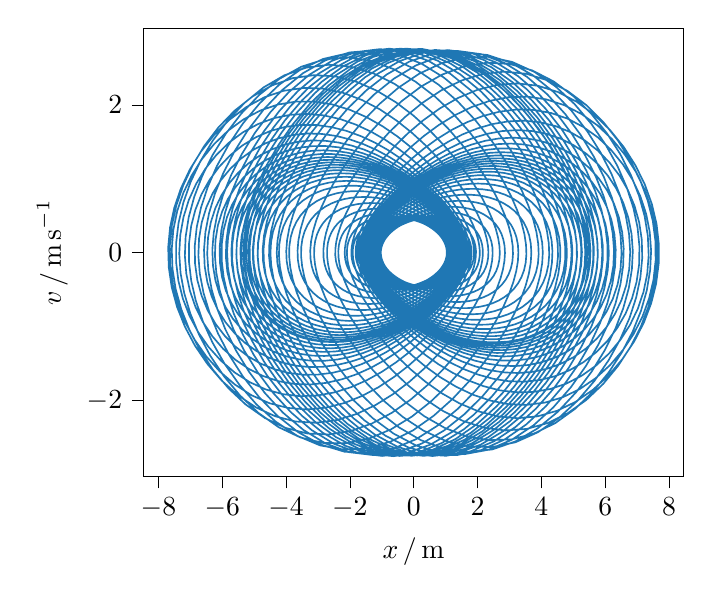
\begin{tikzpicture}

\definecolor{darkgray176}{RGB}{176,176,176}
\definecolor{steelblue31119180}{RGB}{31,119,180}

\begin{axis}[
tick align=outside,
tick pos=left,
x grid style={darkgray176},
xlabel={\(\displaystyle x\,/\,\mathrm{m}\)},
xmin=-8.4616, xmax=8.4476,
xtick style={color=black},
y grid style={darkgray176},
ylabel={\(\displaystyle v\,/\,\mathrm{m\, s^{-1}}\)},
ymin=-3.02975, ymax=3.03675,
ytick style={color=black}
]
\addplot [semithick, steelblue31119180]
table {%
0 1
0.14 0.498
0.279 0.493
0.415 0.483
0.549 0.47
0.678 0.454
0.802 0.433
0.921 0.41
1.032 0.383
1.135 0.352
1.229 0.319
1.313 0.282
1.386 0.242
1.448 0.2
1.498 0.154
1.534 0.106
1.557 0.055
1.565 0.002
1.557 -0.054
1.534 -0.113
1.494 -0.173
1.437 -0.236
1.362 -0.301
1.268 -0.367
1.156 -0.436
1.024 -0.505
0.873 -0.576
0.702 -0.647
0.511 -0.718
0.3 -0.788
0.07 -0.856
-0.179 -0.922
-0.446 -0.984
-0.73 -1.042
-1.029 -1.092
-1.341 -1.136
-1.664 -1.17
-1.995 -1.193
-2.331 -1.204
-2.668 -1.203
-3.003 -1.187
-3.332 -1.157
-3.649 -1.111
-3.953 -1.051
-4.236 -0.975
-4.497 -0.884
-4.73 -0.779
-4.932 -0.659
-5.098 -0.525
-5.224 -0.377
-5.307 -0.215
-5.343 -0.038
-5.327 0.153
-5.256 0.36
-5.124 0.583
-4.928 0.821
-4.663 1.074
-4.325 1.339
-3.912 1.611
-3.423 1.883
-2.859 2.142
-2.226 2.373
-1.534 2.559
-0.798 2.684
-0.038 2.734
0.725 2.703
1.469 2.596
2.173 2.423
2.821 2.201
3.402 1.947
3.91 1.676
4.341 1.402
4.695 1.133
4.976 0.875
5.187 0.632
5.331 0.403
5.414 0.19
5.439 -0.007
5.411 -0.19
5.334 -0.357
5.212 -0.511
5.049 -0.65
4.849 -0.776
4.616 -0.886
4.355 -0.982
4.068 -1.062
3.761 -1.127
3.438 -1.176
3.104 -1.21
2.762 -1.228
2.418 -1.231
2.074 -1.221
1.735 -1.198
1.404 -1.164
1.084 -1.12
0.778 -1.068
0.487 -1.01
0.213 -0.946
-0.043 -0.879
-0.279 -0.808
-0.495 -0.736
-0.691 -0.664
-0.867 -0.591
-1.022 -0.519
-1.157 -0.448
-1.273 -0.378
-1.369 -0.31
-1.446 -0.244
-1.506 -0.18
-1.547 -0.118
-1.572 -0.059
-1.581 -0.002
-1.574 0.052
-1.552 0.103
-1.516 0.152
-1.467 0.198
-1.406 0.241
-1.332 0.281
-1.249 0.318
-1.155 0.352
-1.052 0.382
-0.941 0.409
-0.823 0.433
-0.699 0.453
-0.57 0.47
-0.436 0.483
-0.3 0.492
-0.161 0.498
-0.022 0.499
0.118 0.497
0.257 0.492
0.393 0.482
0.526 0.469
0.656 0.453
0.78 0.433
0.898 0.409
1.008 0.382
1.111 0.352
1.205 0.319
1.29 0.282
1.363 0.243
1.425 0.201
1.475 0.156
1.513 0.109
1.536 0.058
1.545 0.006
1.539 -0.049
1.517 -0.107
1.479 -0.166
1.424 -0.228
1.351 -0.291
1.261 -0.356
1.152 -0.423
1.024 -0.491
0.877 -0.559
0.711 -0.629
0.525 -0.698
0.32 -0.766
0.096 -0.833
-0.146 -0.897
-0.406 -0.957
-0.682 -1.013
-0.973 -1.063
-1.277 -1.106
-1.591 -1.14
-1.914 -1.164
-2.242 -1.177
-2.572 -1.177
-2.9 -1.164
-3.222 -1.137
-3.535 -1.095
-3.834 -1.038
-4.115 -0.967
-4.374 -0.882
-4.607 -0.781
-4.81 -0.667
-4.98 -0.539
-5.111 -0.397
-5.2 -0.24
-5.244 -0.07
-5.238 0.116
-5.178 0.316
-5.059 0.533
-4.878 0.765
-4.629 1.013
-4.31 1.274
-3.915 1.543
-3.445 1.815
-2.9 2.078
-2.284 2.317
-1.606 2.517
-0.879 2.659
-0.123 2.73
0.642 2.72
1.393 2.632
2.109 2.475
2.774 2.263
3.373 2.015
3.9 1.746
4.35 1.47
4.724 1.197
5.022 0.935
5.248 0.685
5.407 0.45
5.502 0.231
5.538 0.028
5.519 -0.161
5.449 -0.335
5.332 -0.494
5.173 -0.639
4.976 -0.77
4.743 -0.886
4.481 -0.987
4.192 -1.073
3.882 -1.142
3.554 -1.195
3.214 -1.232
2.866 -1.253
2.514 -1.258
2.162 -1.249
1.815 -1.227
1.476 -1.193
1.148 -1.149
0.834 -1.097
0.535 -1.037
0.253 -0.971
-0.009 -0.902
-0.251 -0.83
-0.474 -0.756
-0.675 -0.682
-0.855 -0.607
-1.015 -0.533
-1.154 -0.461
-1.273 -0.389
-1.372 -0.32
-1.452 -0.253
-1.514 -0.188
-1.558 -0.125
-1.584 -0.065
-1.594 -0.007
-1.588 0.047
-1.568 0.099
-1.533 0.149
-1.485 0.195
-1.424 0.238
-1.352 0.279
-1.269 0.316
-1.175 0.35
-1.073 0.38
-0.963 0.407
-0.845 0.431
-0.722 0.451
-0.593 0.468
-0.46 0.481
-0.324 0.49
-0.186 0.496
-0.047 0.498
0.093 0.496
0.231 0.49
0.367 0.481
0.5 0.468
0.628 0.451
0.752 0.431
0.87 0.408
0.98 0.382
1.083 0.352
1.177 0.319
1.261 0.283
1.335 0.244
1.398 0.203
1.449 0.159
1.486 0.112
1.511 0.063
1.521 0.011
1.517 -0.043
1.497 -0.099
1.461 -0.157
1.409 -0.217
1.339 -0.279
1.252 -0.343
1.147 -0.408
1.024 -0.474
0.882 -0.541
0.721 -0.608
0.541 -0.675
0.343 -0.741
0.126 -0.806
-0.108 -0.868
-0.36 -0.927
-0.627 -0.982
-0.909 -1.031
-1.204 -1.073
-1.509 -1.107
-1.823 -1.132
-2.142 -1.146
-2.464 -1.149
-2.784 -1.138
-3.1 -1.115
-3.407 -1.077
-3.702 -1.025
-3.98 -0.96
-4.238 -0.879
-4.471 -0.785
-4.676 -0.677
-4.849 -0.555
-4.986 -0.42
-5.083 -0.27
-5.136 -0.106
-5.141 0.072
-5.094 0.266
-4.99 0.476
-4.826 0.701
-4.596 0.943
-4.296 1.198
-3.924 1.465
-3.476 1.736
-2.952 2.002
-2.356 2.25
-1.695 2.463
-0.982 2.625
-0.232 2.719
0.534 2.734
1.292 2.669
2.022 2.531
2.704 2.333
3.324 2.093
3.874 1.827
4.347 1.551
4.742 1.275
5.061 1.006
5.307 0.75
5.483 0.509
5.593 0.283
5.642 0.072
5.635 -0.124
5.575 -0.304
5.466 -0.471
5.312 -0.622
5.118 -0.76
4.888 -0.882
4.626 -0.989
4.336 -1.081
4.022 -1.155
3.69 -1.213
3.344 -1.254
2.989 -1.279
2.63 -1.287
2.27 -1.28
1.914 -1.26
1.566 -1.226
1.228 -1.182
0.905 -1.128
0.597 -1.067
0.307 -1.001
0.037 -0.93
-0.213 -0.855
-0.442 -0.78
-0.649 -0.703
-0.835 -0.627
-1 -0.551
-1.144 -0.476
-1.267 -0.404
-1.37 -0.333
-1.454 -0.264
-1.518 -0.198
-1.565 -0.134
-1.594 -0.073
-1.606 -0.015
-1.602 0.041
-1.583 0.094
-1.55 0.143
-1.503 0.19
-1.444 0.234
-1.373 0.274
-1.291 0.312
-1.198 0.346
-1.097 0.377
-0.988 0.404
-0.871 0.428
-0.749 0.448
-0.621 0.465
-0.489 0.478
-0.353 0.487
-0.216 0.493
-0.078 0.495
0.061 0.493
0.198 0.488
0.333 0.478
0.466 0.466
0.594 0.45
0.717 0.43
0.834 0.407
0.945 0.381
1.048 0.352
1.142 0.319
1.226 0.284
1.3 0.246
1.364 0.206
1.415 0.162
1.454 0.117
1.48 0.068
1.492 0.018
1.49 -0.035
1.473 -0.089
1.44 -0.146
1.391 -0.204
1.325 -0.264
1.243 -0.326
1.143 -0.389
1.025 -0.453
0.889 -0.518
0.735 -0.583
0.562 -0.648
0.372 -0.712
0.164 -0.774
-0.061 -0.835
-0.303 -0.892
-0.561 -0.946
-0.832 -0.994
-1.117 -1.036
-1.412 -1.07
-1.715 -1.096
-2.024 -1.112
-2.336 -1.116
-2.648 -1.11
-2.957 -1.09
-3.258 -1.057
-3.547 -1.011
-3.823 -0.951
-4.079 -0.878
-4.313 -0.79
-4.52 -0.689
-4.698 -0.575
-4.841 -0.447
-4.947 -0.305
-5.011 -0.149
-5.029 0.021
-4.997 0.206
-4.912 0.408
-4.768 0.625
-4.56 0.859
-4.285 1.107
-3.939 1.369
-3.518 1.638
-3.022 1.906
-2.452 2.162
-1.814 2.391
-1.117 2.574
-0.378 2.695
0.385 2.741
1.149 2.706
1.893 2.594
2.595 2.416
3.241 2.188
3.818 1.928
4.319 1.653
4.743 1.373
5.089 1.099
5.359 0.836
5.558 0.586
5.689 0.351
5.756 0.132
5.764 -0.072
5.717 -0.261
5.62 -0.435
5.475 -0.595
5.287 -0.741
5.061 -0.871
4.801 -0.986
4.511 -1.085
4.195 -1.166
3.859 -1.231
3.508 -1.278
3.145 -1.307
2.777 -1.319
2.408 -1.316
2.042 -1.297
1.683 -1.265
1.335 -1.221
1 -1.167
0.682 -1.105
0.382 -1.036
0.102 -0.963
-0.157 -0.887
-0.394 -0.809
-0.61 -0.731
-0.803 -0.652
-0.975 -0.574
-1.125 -0.497
-1.254 -0.423
-1.362 -0.35
-1.45 -0.28
-1.519 -0.212
-1.569 -0.147
-1.601 -0.085
-1.617 -0.025
-1.616 0.031
-1.599 0.085
-1.569 0.135
-1.524 0.182
-1.467 0.227
-1.397 0.268
-1.317 0.305
-1.227 0.34
-1.127 0.371
-1.019 0.399
-0.904 0.423
-0.783 0.443
-0.656 0.46
-0.525 0.473
-0.391 0.483
-0.255 0.489
-0.118 0.491
0.019 0.489
0.156 0.484
0.29 0.476
0.422 0.463
0.549 0.448
0.672 0.429
0.789 0.406
0.899 0.381
1.002 0.352
1.096 0.321
1.181 0.287
1.257 0.25
1.321 0.21
1.374 0.168
1.415 0.123
1.443 0.077
1.457 0.028
1.458 -0.023
1.444 -0.076
1.415 -0.131
1.371 -0.187
1.31 -0.246
1.233 -0.305
1.139 -0.366
1.028 -0.427
0.9 -0.489
0.754 -0.552
0.591 -0.614
0.41 -0.676
0.212 -0.736
-0.002 -0.795
-0.232 -0.85
-0.478 -0.902
-0.737 -0.95
-1.009 -0.991
-1.292 -1.026
-1.583 -1.053
-1.881 -1.071
-2.182 -1.079
-2.484 -1.076
-2.783 -1.061
-3.077 -1.034
-3.361 -0.994
-3.632 -0.941
-3.887 -0.876
-4.121 -0.796
-4.332 -0.704
-4.515 -0.598
-4.666 -0.48
-4.782 -0.347
-4.859 -0.201
-4.893 -0.041
-4.88 0.134
-4.816 0.325
-4.697 0.532
-4.517 0.756
-4.272 0.995
-3.958 1.249
-3.572 1.513
-3.11 1.782
-2.574 2.045
-1.967 2.288
-1.296 2.495
-0.575 2.648
0.18 2.731
0.947 2.735
1.704 2.659
2.429 2.51
3.104 2.303
3.715 2.055
4.253 1.784
4.713 1.502
5.095 1.223
5.399 0.951
5.628 0.691
5.787 0.446
5.879 0.217
5.91 0.002
5.882 -0.197
5.801 -0.382
5.669 -0.553
5.492 -0.708
5.274 -0.849
5.019 -0.973
4.73 -1.082
4.414 -1.173
4.075 -1.246
3.718 -1.301
3.348 -1.337
2.971 -1.356
2.591 -1.357
2.213 -1.341
1.841 -1.311
1.48 -1.268
1.132 -1.215
0.8 -1.152
0.487 -1.082
0.195 -1.007
-0.076 -0.929
-0.325 -0.848
-0.551 -0.767
-0.755 -0.685
-0.935 -0.605
-1.093 -0.526
-1.23 -0.449
-1.345 -0.374
-1.439 -0.301
-1.514 -0.232
-1.569 -0.165
-1.606 -0.101
-1.626 -0.041
-1.629 0.017
-1.617 0.072
-1.589 0.123
-1.548 0.171
-1.494 0.216
-1.427 0.258
-1.35 0.296
-1.262 0.331
-1.165 0.363
-1.059 0.391
-0.946 0.415
-0.827 0.436
-0.702 0.453
-0.573 0.467
-0.441 0.477
-0.306 0.483
-0.171 0.486
-0.035 0.485
0.101 0.48
0.234 0.472
0.365 0.461
0.492 0.446
0.614 0.427
0.731 0.406
0.841 0.381
0.944 0.354
1.039 0.324
1.125 0.29
1.201 0.255
1.267 0.216
1.322 0.176
1.366 0.133
1.397 0.088
1.415 0.041
1.419 -0.008
1.41 -0.059
1.386 -0.112
1.347 -0.166
1.293 -0.222
1.223 -0.278
1.137 -0.336
1.034 -0.395
0.915 -0.455
0.78 -0.514
0.627 -0.574
0.458 -0.633
0.273 -0.691
0.072 -0.747
-0.145 -0.801
-0.376 -0.851
-0.621 -0.897
-0.878 -0.939
-1.146 -0.974
-1.423 -1.002
-1.707 -1.022
-1.995 -1.033
-2.284 -1.035
-2.573 -1.025
-2.857 -1.005
-3.135 -0.972
-3.401 -0.928
-3.653 -0.871
-3.887 -0.801
-4.101 -0.719
-4.289 -0.624
-4.449 -0.516
-4.577 -0.395
-4.669 -0.261
-4.722 -0.113
-4.731 0.05
-4.692 0.228
-4.602 0.421
-4.455 0.632
-4.247 0.858
-3.973 1.101
-3.629 1.357
-3.212 1.622
-2.72 1.888
-2.155 2.144
-1.522 2.374
-0.83 2.562
-0.093 2.69
0.67 2.743
1.436 2.716
2.183 2.61
2.891 2.436
3.543 2.211
4.126 1.95
4.633 1.671
5.061 1.387
5.41 1.107
5.682 0.837
5.88 0.579
6.008 0.336
6.07 0.109
6.07 -0.104
6.013 -0.302
5.902 -0.485
5.742 -0.654
5.537 -0.808
5.291 -0.946
5.009 -1.067
4.695 -1.171
4.355 -1.256
3.994 -1.322
3.616 -1.369
3.229 -1.396
2.836 -1.405
2.444 -1.395
2.056 -1.369
1.678 -1.329
1.313 -1.276
0.964 -1.213
0.634 -1.142
0.325 -1.065
0.038 -0.984
-0.226 -0.9
-0.466 -0.816
-0.682 -0.731
-0.875 -0.647
-1.045 -0.564
-1.192 -0.484
-1.316 -0.406
-1.419 -0.331
-1.502 -0.259
-1.565 -0.19
-1.609 -0.125
-1.635 -0.062
-1.644 -0.003
-1.637 0.053
-1.614 0.106
-1.578 0.156
-1.527 0.202
-1.465 0.244
-1.391 0.283
-1.307 0.319
-1.213 0.351
-1.11 0.38
-1 0.405
-0.883 0.427
-0.761 0.445
-0.635 0.459
-0.505 0.47
-0.372 0.477
-0.238 0.48
-0.104 0.48
0.03 0.476
0.163 0.469
0.292 0.458
0.419 0.444
0.541 0.427
0.657 0.406
0.768 0.383
0.871 0.357
0.967 0.328
1.055 0.296
1.133 0.262
1.201 0.225
1.259 0.186
1.305 0.145
1.34 0.102
1.362 0.057
1.372 0.011
1.368 -0.038
1.351 -0.088
1.319 -0.139
1.273 -0.192
1.211 -0.246
1.135 -0.301
1.042 -0.357
0.935 -0.413
0.811 -0.47
0.672 -0.526
0.516 -0.582
0.346 -0.637
0.16 -0.69
-0.041 -0.742
-0.255 -0.79
-0.483 -0.835
-0.722 -0.876
-0.973 -0.911
-1.232 -0.941
-1.499 -0.963
-1.771 -0.978
-2.046 -0.984
-2.321 -0.98
-2.594 -0.967
-2.862 -0.943
-3.121 -0.907
-3.369 -0.86
-3.602 -0.802
-3.816 -0.731
-4.01 -0.649
-4.178 -0.554
-4.319 -0.446
-4.427 -0.326
-4.5 -0.193
-4.534 -0.045
-4.524 0.117
-4.467 0.294
-4.358 0.487
-4.192 0.697
-3.966 0.924
-3.673 1.166
-3.311 1.422
-2.876 1.685
-2.368 1.947
-1.787 2.197
-1.14 2.418
-0.438 2.593
0.306 2.705
1.07 2.741
1.833 2.697
2.573 2.575
3.269 2.388
3.906 2.153
4.472 1.886
4.961 1.603
5.369 1.317
5.699 1.035
5.95 0.764
6.128 0.506
6.235 0.262
6.276 0.033
6.254 -0.182
6.175 -0.382
6.042 -0.567
5.859 -0.738
5.63 -0.893
5.36 -1.032
5.054 -1.153
4.717 -1.255
4.353 -1.337
3.97 -1.399
3.571 -1.44
3.165 -1.46
2.756 -1.46
2.349 -1.442
1.95 -1.406
1.563 -1.356
1.191 -1.294
0.839 -1.223
0.507 -1.143
0.199 -1.059
-0.085 -0.972
-0.345 -0.883
-0.58 -0.793
-0.789 -0.705
-0.974 -0.618
-1.135 -0.533
-1.273 -0.452
-1.389 -0.373
-1.482 -0.297
-1.555 -0.225
-1.609 -0.156
-1.643 -0.091
-1.66 -0.029
-1.66 0.029
-1.644 0.083
-1.614 0.134
-1.569 0.182
-1.512 0.226
-1.443 0.267
-1.363 0.304
-1.273 0.337
-1.175 0.367
-1.068 0.393
-0.955 0.415
-0.836 0.434
-0.712 0.449
-0.585 0.461
-0.455 0.469
-0.323 0.473
-0.19 0.474
-0.058 0.471
0.073 0.465
0.202 0.455
0.328 0.442
0.449 0.426
0.566 0.407
0.677 0.386
0.782 0.361
0.879 0.333
0.968 0.304
1.049 0.271
1.12 0.237
1.181 0.2
1.232 0.161
1.271 0.12
1.299 0.078
1.315 0.034
1.318 -0.012
1.308 -0.059
1.284 -0.108
1.247 -0.158
1.196 -0.208
1.13 -0.26
1.05 -0.312
0.955 -0.365
0.846 -0.418
0.721 -0.471
0.582 -0.523
0.428 -0.575
0.26 -0.625
0.078 -0.674
-0.117 -0.72
-0.325 -0.763
-0.544 -0.803
-0.774 -0.839
-1.013 -0.869
-1.26 -0.893
-1.513 -0.911
-1.769 -0.921
-2.028 -0.924
-2.286 -0.917
-2.541 -0.901
-2.789 -0.875
-3.03 -0.839
-3.258 -0.793
-3.473 -0.735
-3.669 -0.666
-3.844 -0.586
-3.996 -0.494
-4.12 -0.39
-4.213 -0.273
-4.272 -0.144
-4.292 -0.001
-4.271 0.157
-4.203 0.329
-4.085 0.518
-3.911 0.724
-3.678 0.946
-3.38 1.184
-3.014 1.434
-2.576 1.693
-2.066 1.951
-1.485 2.196
-0.839 2.413
-0.138 2.585
0.603 2.695
1.365 2.73
2.124 2.685
2.861 2.563
3.554 2.377
4.187 2.141
4.75 1.874
5.235 1.59
5.64 1.301
5.964 1.017
6.21 0.742
6.381 0.48
6.48 0.231
6.512 -0.004
6.479 -0.224
6.387 -0.431
6.239 -0.623
6.04 -0.8
5.793 -0.961
5.503 -1.105
5.176 -1.231
4.816 -1.336
4.429 -1.42
4.023 -1.481
3.602 -1.52
3.174 -1.535
2.744 -1.529
2.319 -1.503
1.904 -1.46
1.503 -1.401
1.121 -1.329
0.76 -1.249
0.422 -1.161
0.11 -1.069
-0.176 -0.974
-0.436 -0.879
-0.669 -0.785
-0.875 -0.692
-1.056 -0.601
-1.212 -0.513
-1.344 -0.429
-1.453 -0.349
-1.54 -0.272
-1.606 -0.199
-1.652 -0.13
-1.679 -0.065
-1.688 -0.004
-1.681 0.054
-1.659 0.107
-1.622 0.157
-1.571 0.203
-1.508 0.246
-1.434 0.284
-1.349 0.319
-1.255 0.35
-1.153 0.378
-1.044 0.402
-0.929 0.422
-0.808 0.438
-0.684 0.451
-0.556 0.46
-0.426 0.465
-0.296 0.467
-0.165 0.466
-0.035 0.461
0.093 0.453
0.218 0.442
0.34 0.427
0.457 0.41
0.569 0.389
0.675 0.366
0.774 0.341
0.866 0.313
0.949 0.283
1.024 0.25
1.089 0.216
1.144 0.179
1.189 0.141
1.223 0.101
1.246 0.06
1.256 0.017
1.255 -0.027
1.241 -0.073
1.214 -0.119
1.174 -0.166
1.121 -0.214
1.054 -0.263
0.974 -0.312
0.88 -0.361
0.772 -0.41
0.65 -0.458
0.515 -0.506
0.367 -0.553
0.206 -0.599
0.032 -0.642
-0.154 -0.683
-0.35 -0.721
-0.557 -0.756
-0.773 -0.786
-0.997 -0.812
-1.228 -0.832
-1.463 -0.846
-1.701 -0.853
-1.94 -0.853
-2.178 -0.845
-2.412 -0.829
-2.641 -0.803
-2.861 -0.768
-3.07 -0.724
-3.266 -0.669
-3.444 -0.605
-3.603 -0.529
-3.74 -0.443
-3.85 -0.345
-3.932 -0.236
-3.981 -0.114
-3.994 0.021
-3.968 0.17
-3.898 0.334
-3.779 0.514
-3.608 0.71
-3.38 0.922
-3.091 1.15
-2.735 1.391
-2.311 1.641
-1.816 1.893
-1.251 2.136
-0.622 2.354
0.063 2.532
0.791 2.653
1.542 2.704
2.297 2.676
3.034 2.572
3.731 2.401
4.373 2.177
4.947 1.918
5.445 1.637
5.863 1.349
6.2 1.061
6.458 0.781
6.639 0.511
6.746 0.254
6.782 0.009
6.752 -0.222
6.659 -0.44
6.507 -0.644
6.3 -0.833
6.042 -1.007
5.738 -1.163
5.392 -1.299
5.012 -1.414
4.603 -1.505
4.171 -1.572
3.725 -1.613
3.27 -1.629
2.815 -1.62
2.365 -1.589
1.927 -1.538
1.505 -1.471
1.104 -1.39
0.728 -1.3
0.377 -1.202
0.055 -1.101
-0.239 -0.998
-0.504 -0.895
-0.74 -0.793
-0.949 -0.694
-1.129 -0.598
-1.284 -0.506
-1.413 -0.419
-1.519 -0.335
-1.601 -0.256
-1.662 -0.182
-1.703 -0.111
-1.725 -0.046
-1.729 0.016
-1.717 0.073
-1.689 0.127
-1.646 0.176
-1.591 0.221
-1.523 0.262
-1.444 0.299
-1.356 0.332
-1.259 0.362
-1.154 0.387
-1.042 0.409
-0.925 0.427
-0.803 0.441
-0.678 0.452
-0.55 0.459
-0.421 0.462
-0.292 0.462
-0.163 0.459
-0.035 0.452
0.09 0.442
0.212 0.43
0.33 0.414
0.444 0.395
0.551 0.374
0.653 0.35
0.747 0.324
0.834 0.296
0.913 0.266
0.983 0.234
1.044 0.2
1.095 0.164
1.135 0.127
1.165 0.088
1.185 0.048
1.192 0.007
1.189 -0.035
1.173 -0.078
1.145 -0.121
1.105 -0.166
1.052 -0.211
0.987 -0.256
0.909 -0.301
0.818 -0.346
0.715 -0.39
0.6 -0.435
0.472 -0.478
0.332 -0.52
0.181 -0.56
0.019 -0.598
-0.154 -0.634
-0.336 -0.667
-0.527 -0.697
-0.726 -0.723
-0.931 -0.744
-1.142 -0.761
-1.357 -0.772
-1.574 -0.777
-1.791 -0.775
-2.007 -0.766
-2.22 -0.75
-2.426 -0.726
-2.625 -0.694
-2.814 -0.653
-2.99 -0.603
-3.151 -0.544
-3.294 -0.475
-3.416 -0.397
-3.515 -0.308
-3.588 -0.208
-3.63 -0.096
-3.64 0.028
-3.614 0.165
-3.547 0.316
-3.436 0.481
-3.276 0.662
-3.063 0.859
-2.793 1.071
-2.462 1.298
-2.066 1.534
-1.602 1.775
-1.072 2.012
-0.477 2.233
0.176 2.422
0.875 2.563
1.605 2.642
2.348 2.649
3.082 2.581
3.787 2.444
4.445 2.248
5.042 2.009
5.567 1.741
6.015 1.459
6.384 1.171
6.671 0.886
6.881 0.608
7.013 0.34
7.072 0.083
7.061 -0.163
6.982 -0.396
6.84 -0.618
6.637 -0.825
6.379 -1.018
6.069 -1.194
5.712 -1.35
5.315 -1.483
4.884 -1.591
4.426 -1.672
3.95 -1.724
3.464 -1.746
2.975 -1.74
2.492 -1.707
2.021 -1.651
1.569 -1.576
1.14 -1.486
0.738 -1.384
0.366 -1.275
0.024 -1.162
-0.285 -1.047
-0.562 -0.934
-0.808 -0.822
-1.023 -0.715
-1.209 -0.611
-1.366 -0.513
-1.496 -0.419
-1.601 -0.331
-1.682 -0.248
-1.741 -0.171
-1.778 -0.098
-1.796 -0.03
-1.796 0.032
-1.779 0.09
-1.746 0.144
-1.698 0.193
-1.638 0.238
-1.565 0.278
-1.482 0.314
-1.39 0.347
-1.289 0.375
-1.18 0.399
-1.066 0.419
-0.946 0.435
-0.823 0.447
-0.696 0.456
-0.568 0.461
-0.438 0.462
-0.309 0.46
-0.181 0.455
-0.055 0.447
0.069 0.436
0.189 0.421
0.305 0.404
0.415 0.385
0.52 0.363
0.618 0.338
0.709 0.312
0.793 0.284
0.868 0.254
0.935 0.222
0.992 0.188
1.04 0.154
1.078 0.117
1.106 0.08
1.123 0.042
1.129 0.003
1.124 -0.037
1.108 -0.077
1.081 -0.118
1.042 -0.159
0.992 -0.201
0.93 -0.242
0.856 -0.283
0.771 -0.324
0.675 -0.365
0.567 -0.404
0.449 -0.442
0.319 -0.479
0.18 -0.515
0.031 -0.548
-0.126 -0.579
-0.292 -0.607
-0.466 -0.632
-0.646 -0.654
-0.832 -0.671
-1.022 -0.684
-1.214 -0.692
-1.409 -0.695
-1.603 -0.692
-1.796 -0.683
-1.985 -0.668
-2.169 -0.646
-2.346 -0.616
-2.514 -0.579
-2.67 -0.535
-2.812 -0.482
-2.939 -0.42
-3.047 -0.35
-3.134 -0.271
-3.197 -0.181
-3.234 -0.082
-3.242 0.029
-3.217 0.152
-3.156 0.287
-3.055 0.435
-2.911 0.597
-2.719 0.774
-2.476 0.966
-2.177 1.171
-1.819 1.388
-1.399 1.611
-0.916 1.836
-0.372 2.052
0.231 2.248
0.884 2.408
1.575 2.52
2.289 2.57
3.008 2.553
3.712 2.466
4.383 2.317
5.005 2.117
5.565 1.878
6.054 1.614
6.467 1.336
6.802 1.053
7.057 0.771
7.234 0.495
7.335 0.226
7.361 -0.035
7.316 -0.287
7.201 -0.529
7.02 -0.76
6.777 -0.978
6.474 -1.181
6.117 -1.366
5.711 -1.528
5.264 -1.665
4.782 -1.772
4.274 -1.846
3.751 -1.885
3.222 -1.89
2.696 -1.863
2.182 -1.806
1.687 -1.725
1.217 -1.625
0.778 -1.511
0.372 -1.387
0.002 -1.259
-0.332 -1.129
-0.631 -1.001
-0.893 -0.876
-1.121 -0.756
-1.317 -0.641
-1.481 -0.533
-1.616 -0.431
-1.723 -0.336
-1.804 -0.247
-1.862 -0.164
-1.897 -0.087
-1.911 -0.016
-1.906 0.049
-1.884 0.109
-1.846 0.164
-1.792 0.214
-1.726 0.26
-1.648 0.3
-1.558 0.336
-1.46 0.367
-1.353 0.394
-1.24 0.417
-1.12 0.435
-0.996 0.45
-0.869 0.46
-0.739 0.467
-0.607 0.47
-0.476 0.47
-0.345 0.466
-0.215 0.459
-0.088 0.449
0.036 0.436
0.156 0.42
0.271 0.401
0.38 0.381
0.484 0.358
0.58 0.332
0.67 0.305
0.751 0.277
0.825 0.246
0.889 0.215
0.945 0.182
0.991 0.147
1.027 0.112
1.053 0.076
1.07 0.039
1.075 0.002
1.071 -0.036
1.055 -0.074
1.029 -0.112
0.992 -0.151
0.945 -0.189
0.887 -0.227
0.818 -0.265
0.738 -0.302
0.649 -0.338
0.549 -0.373
0.44 -0.407
0.322 -0.439
0.194 -0.47
0.059 -0.499
-0.085 -0.525
-0.235 -0.549
-0.392 -0.569
-0.554 -0.587
-0.72 -0.6
-0.89 -0.61
-1.061 -0.616
-1.234 -0.616
-1.406 -0.612
-1.576 -0.603
-1.743 -0.588
-1.905 -0.567
-2.06 -0.539
-2.206 -0.506
-2.342 -0.465
-2.466 -0.418
-2.576 -0.363
-2.669 -0.301
-2.743 -0.23
-2.797 -0.151
-2.827 -0.063
-2.831 0.035
-2.807 0.142
-2.751 0.261
-2.66 0.391
-2.53 0.534
-2.36 0.689
-2.144 0.857
-1.879 1.037
-1.562 1.228
-1.19 1.428
-0.761 1.633
-0.276 1.834
0.265 2.025
0.856 2.194
1.49 2.328
2.156 2.417
2.838 2.449
3.522 2.421
4.188 2.332
4.822 2.187
5.409 1.996
5.937 1.769
6.397 1.518
6.785 1.252
7.097 0.978
7.333 0.702
7.491 0.428
7.573 0.157
7.579 -0.108
7.512 -0.369
7.373 -0.622
7.165 -0.867
6.889 -1.102
6.549 -1.321
6.151 -1.522
5.699 -1.699
5.202 -1.846
4.669 -1.957
4.11 -2.029
3.536 -2.06
2.96 -2.05
2.392 -2.001
1.842 -1.92
1.319 -1.812
0.829 -1.685
0.377 -1.544
-0.035 -1.397
-0.405 -1.247
-0.733 -1.1
-1.021 -0.956
-1.269 -0.819
-1.48 -0.689
-1.656 -0.567
-1.799 -0.453
-1.911 -0.348
-1.994 -0.249
-2.051 -0.159
-2.084 -0.076
-2.094 0.001
-2.084 0.071
-2.055 0.135
-2.009 0.193
-1.947 0.245
-1.872 0.291
-1.785 0.332
-1.687 0.369
-1.579 0.4
-1.463 0.426
-1.341 0.448
-1.213 0.465
-1.08 0.478
-0.945 0.487
-0.808 0.492
-0.67 0.493
-0.532 0.49
-0.396 0.484
-0.262 0.475
-0.13 0.462
-0.003 0.447
0.12 0.429
0.237 0.408
0.348 0.386
0.453 0.361
0.55 0.334
0.64 0.306
0.721 0.276
0.794 0.245
0.859 0.213
0.913 0.179
0.959 0.145
0.995 0.11
1.021 0.075
1.036 0.039
1.042 0.002
1.038 -0.034
1.023 -0.071
0.998 -0.107
0.963 -0.144
0.917 -0.18
0.862 -0.215
0.797 -0.25
0.722 -0.284
0.638 -0.316
0.545 -0.348
0.444 -0.378
0.334 -0.407
0.216 -0.434
0.091 -0.458
-0.041 -0.48
-0.178 -0.5
-0.32 -0.517
-0.467 -0.531
-0.617 -0.541
-0.77 -0.548
-0.923 -0.55
-1.077 -0.549
-1.23 -0.543
-1.381 -0.532
-1.528 -0.517
-1.67 -0.496
-1.806 -0.47
-1.933 -0.439
-2.051 -0.402
-2.157 -0.358
-2.251 -0.308
-2.33 -0.252
-2.391 -0.189
-2.435 -0.118
-2.457 -0.04
-2.456 0.046
-2.43 0.141
-2.376 0.245
-2.292 0.359
-2.174 0.483
-2.021 0.617
-1.828 0.762
-1.593 0.918
-1.313 1.083
-0.985 1.257
-0.609 1.435
-0.182 1.615
0.295 1.79
0.82 1.952
1.387 2.093
1.989 2.202
2.616 2.27
3.256 2.29
3.894 2.258
4.516 2.174
5.107 2.041
5.655 1.867
6.149 1.66
6.582 1.428
6.948 1.18
7.242 0.921
7.463 0.655
7.609 0.387
7.679 0.118
7.675 -0.151
7.595 -0.419
7.441 -0.684
7.213 -0.944
6.913 -1.197
6.544 -1.437
6.11 -1.659
5.617 -1.855
5.074 -2.018
4.491 -2.14
3.88 -2.215
3.255 -2.24
2.63 -2.216
2.019 -2.146
1.432 -2.039
0.879 -1.903
0.368 -1.747
-0.098 -1.579
-0.516 -1.406
-0.885 -1.234
-1.207 -1.067
-1.483 -0.908
-1.716 -0.758
-1.909 -0.618
-2.063 -0.487
-2.183 -0.367
-2.27 -0.256
-2.327 -0.155
-2.357 -0.062
-2.363 0.022
-2.346 0.099
-2.308 0.169
-2.252 0.231
-2.179 0.287
-2.092 0.336
-1.991 0.38
-1.88 0.417
-1.758 0.449
-1.629 0.476
-1.493 0.497
-1.351 0.513
-1.206 0.525
-1.058 0.532
-0.908 0.534
-0.759 0.533
-0.61 0.528
-0.464 0.519
-0.32 0.506
-0.18 0.491
-0.045 0.473
0.084 0.452
0.207 0.428
0.324 0.403
0.433 0.376
0.534 0.347
0.627 0.316
0.711 0.284
0.786 0.251
0.851 0.217
0.907 0.182
0.953 0.147
0.989 0.111
1.016 0.075
1.031 0.039
1.037 0.003
1.033 -0.034
1.018 -0.07
0.994 -0.105
0.959 -0.141
0.915 -0.175
0.861 -0.209
0.798 -0.242
0.726 -0.273
0.645 -0.304
0.556 -0.333
0.459 -0.36
0.354 -0.386
0.243 -0.41
0.125 -0.431
0.002 -0.45
-0.127 -0.467
-0.259 -0.48
-0.395 -0.491
-0.534 -0.498
-0.674 -0.502
-0.815 -0.502
-0.955 -0.499
-1.094 -0.491
-1.23 -0.479
-1.362 -0.463
-1.489 -0.442
-1.609 -0.416
-1.721 -0.386
-1.824 -0.35
-1.916 -0.309
-1.997 -0.262
-2.063 -0.21
-2.114 -0.152
-2.147 -0.088
-2.162 -0.017
-2.156 0.061
-2.127 0.146
-2.074 0.238
-1.993 0.338
-1.884 0.447
-1.743 0.564
-1.567 0.689
-1.356 0.823
-1.105 0.965
-0.814 1.114
-0.481 1.268
-0.104 1.424
0.316 1.578
0.779 1.725
1.281 1.858
1.818 1.971
2.382 2.054
2.965 2.103
3.556 2.111
4.143 2.075
4.714 1.996
5.257 1.876
5.762 1.72
6.218 1.534
6.618 1.324
6.957 1.096
7.231 0.854
7.435 0.603
7.568 0.345
7.628 0.082
7.613 -0.186
7.523 -0.457
7.357 -0.73
7.114 -1.003
6.796 -1.272
6.403 -1.532
5.939 -1.775
5.411 -1.992
4.827 -2.172
4.199 -2.306
3.541 -2.385
2.869 -2.406
2.199 -2.368
1.547 -2.278
0.927 -2.145
0.349 -1.981
-0.18 -1.795
-0.655 -1.6
-1.076 -1.403
-1.441 -1.209
-1.754 -1.024
-2.016 -0.85
-2.231 -0.687
-2.402 -0.537
-2.532 -0.398
-2.626 -0.272
-2.685 -0.156
-2.714 -0.051
-2.715 0.045
-2.69 0.131
-2.642 0.208
-2.574 0.277
-2.488 0.339
-2.385 0.393
-2.268 0.44
-2.139 0.48
-2 0.514
-1.852 0.541
-1.697 0.563
-1.537 0.579
-1.374 0.589
-1.208 0.595
-1.041 0.595
-0.875 0.591
-0.71 0.583
-0.549 0.571
-0.391 0.555
-0.239 0.536
-0.092 0.514
0.049 0.489
0.182 0.462
0.307 0.433
0.424 0.402
0.532 0.369
0.631 0.335
0.72 0.3
0.799 0.265
0.868 0.228
0.927 0.191
0.975 0.153
1.012 0.116
1.04 0.078
1.056 0.04
1.062 0.003
1.058 -0.034
1.043 -0.07
1.019 -0.106
0.984 -0.141
0.939 -0.176
0.886 -0.209
0.823 -0.241
0.751 -0.271
0.671 -0.301
0.583 -0.328
0.487 -0.354
0.385 -0.378
0.276 -0.399
0.161 -0.418
0.042 -0.435
-0.082 -0.449
-0.209 -0.46
-0.34 -0.468
-0.471 -0.473
-0.604 -0.475
-0.737 -0.473
-0.869 -0.467
-0.998 -0.458
-1.125 -0.444
-1.247 -0.427
-1.363 -0.405
-1.473 -0.379
-1.575 -0.348
-1.668 -0.313
-1.75 -0.273
-1.82 -0.228
-1.877 -0.179
-1.92 -0.124
-1.946 -0.064
-1.955 0.002
-1.944 0.074
-1.913 0.151
-1.859 0.235
-1.781 0.325
-1.676 0.422
-1.544 0.526
-1.381 0.637
-1.187 0.754
-0.958 0.878
-0.695 1.007
-0.394 1.14
-0.056 1.274
0.319 1.408
0.732 1.538
1.18 1.658
1.659 1.763
2.165 1.849
2.692 1.908
3.231 1.937
3.773 1.931
4.309 1.889
4.828 1.812
5.32 1.699
5.777 1.557
6.19 1.387
6.552 1.195
6.857 0.986
7.102 0.761
7.282 0.525
7.395 0.279
7.438 0.023
7.407 -0.24
7.302 -0.511
7.12 -0.788
6.86 -1.069
6.522 -1.349
6.105 -1.623
5.614 -1.882
5.054 -2.114
4.434 -2.307
3.767 -2.448
3.069 -2.526
2.359 -2.538
1.654 -2.485
0.973 -2.372
0.33 -2.213
-0.264 -2.021
-0.8 -1.81
-1.276 -1.591
-1.691 -1.372
-2.046 -1.161
-2.342 -0.961
-2.585 -0.774
-2.777 -0.602
-2.923 -0.443
-3.027 -0.298
-3.091 -0.166
-3.121 -0.046
-3.118 0.062
-3.087 0.16
-3.029 0.248
-2.949 0.326
-2.848 0.395
-2.729 0.455
-2.594 0.508
-2.445 0.552
-2.285 0.589
-2.116 0.618
-1.939 0.641
-1.758 0.657
-1.572 0.667
-1.384 0.671
-1.197 0.67
-1.01 0.663
-0.826 0.652
-0.645 0.636
-0.47 0.616
-0.301 0.593
-0.138 0.566
0.016 0.537
0.162 0.506
0.299 0.472
0.426 0.437
0.543 0.4
0.65 0.362
0.746 0.323
0.831 0.283
0.905 0.243
0.967 0.203
1.018 0.163
1.058 0.122
1.087 0.082
1.104 0.042
1.111 0.003
1.106 -0.035
1.091 -0.073
1.065 -0.11
1.029 -0.146
0.984 -0.181
0.928 -0.214
0.864 -0.246
0.791 -0.276
0.709 -0.305
0.62 -0.332
0.524 -0.357
0.421 -0.379
0.312 -0.399
0.197 -0.417
0.078 -0.432
-0.044 -0.444
-0.17 -0.454
-0.298 -0.46
-0.427 -0.463
-0.557 -0.462
-0.686 -0.458
-0.813 -0.451
-0.938 -0.439
-1.059 -0.424
-1.175 -0.405
-1.285 -0.382
-1.389 -0.355
-1.484 -0.324
-1.57 -0.289
-1.645 -0.249
-1.709 -0.205
-1.76 -0.157
-1.796 -0.104
-1.817 -0.046
-1.822 0.017
-1.808 0.084
-1.774 0.157
-1.719 0.235
-1.642 0.318
-1.54 0.407
-1.413 0.502
-1.259 0.602
-1.076 0.707
-0.862 0.817
-0.618 0.931
-0.341 1.048
-0.031 1.166
0.312 1.284
0.688 1.397
1.094 1.504
1.529 1.6
1.989 1.68
2.468 1.74
2.961 1.776
3.46 1.785
3.957 1.764
4.445 1.712
4.913 1.63
5.355 1.52
5.762 1.383
6.127 1.223
6.445 1.044
6.71 0.847
6.917 0.635
7.064 0.41
7.146 0.173
7.159 -0.076
7.102 -0.335
6.971 -0.605
6.763 -0.883
6.475 -1.168
6.108 -1.455
5.661 -1.736
5.137 -2.001
4.543 -2.238
3.888 -2.431
3.187 -2.566
2.458 -2.631
1.72 -2.624
0.995 -2.546
0.301 -2.407
-0.348 -2.221
-0.94 -2.004
-1.469 -1.77
-1.931 -1.533
-2.327 -1.3
-2.66 -1.077
-2.932 -0.868
-3.147 -0.674
-3.31 -0.495
-3.426 -0.332
-3.497 -0.183
-3.529 -0.048
-3.525 0.074
-3.489 0.184
-3.423 0.283
-3.331 0.371
-3.216 0.449
-3.081 0.517
-2.928 0.576
-2.759 0.625
-2.578 0.666
-2.387 0.699
-2.188 0.724
-1.982 0.741
-1.774 0.75
-1.563 0.753
-1.352 0.75
-1.143 0.741
-0.938 0.726
-0.737 0.706
-0.543 0.682
-0.356 0.655
-0.177 0.623
-0.007 0.589
0.153 0.553
0.303 0.514
0.441 0.474
0.568 0.432
0.683 0.39
0.786 0.347
0.877 0.303
0.956 0.259
1.022 0.215
1.076 0.171
1.118 0.128
1.148 0.085
1.166 0.043
1.172 0.001
1.166 -0.039
1.15 -0.079
1.122 -0.117
1.084 -0.154
1.036 -0.19
0.978 -0.224
0.911 -0.256
0.835 -0.287
0.75 -0.315
0.658 -0.342
0.559 -0.366
0.454 -0.388
0.343 -0.407
0.226 -0.423
0.106 -0.437
-0.018 -0.448
-0.145 -0.455
-0.273 -0.46
-0.402 -0.461
-0.53 -0.459
-0.658 -0.453
-0.784 -0.443
-0.906 -0.43
-1.024 -0.413
-1.137 -0.393
-1.244 -0.368
-1.343 -0.34
-1.434 -0.308
-1.515 -0.272
-1.586 -0.232
-1.645 -0.188
-1.691 -0.139
-1.722 -0.087
-1.739 -0.03
-1.739 0.03
-1.722 0.096
-1.685 0.165
-1.628 0.24
-1.55 0.319
-1.45 0.402
-1.325 0.49
-1.174 0.583
-0.998 0.68
-0.793 0.78
-0.561 0.884
-0.299 0.989
-0.007 1.095
0.314 1.199
0.665 1.301
1.042 1.395
1.445 1.481
1.87 1.553
2.313 1.609
2.769 1.645
3.232 1.658
3.695 1.646
4.152 1.608
4.593 1.544
5.014 1.453
5.405 1.339
5.761 1.202
6.076 1.045
6.344 0.87
6.562 0.679
6.723 0.473
6.825 0.254
6.864 0.021
6.836 -0.224
6.737 -0.483
6.564 -0.753
6.315 -1.033
5.985 -1.321
5.575 -1.61
5.084 -1.891
4.518 -2.152
3.882 -2.378
3.191 -2.554
2.459 -2.663
1.706 -2.696
0.956 -2.653
0.228 -2.538
-0.46 -2.365
-1.093 -2.151
-1.662 -1.912
-2.163 -1.663
-2.593 -1.414
-2.955 -1.174
-3.252 -0.947
-3.487 -0.735
-3.665 -0.54
-3.791 -0.361
-3.869 -0.197
-3.903 -0.049
-3.897 0.086
-3.856 0.208
-3.782 0.317
-3.679 0.414
-3.551 0.501
-3.4 0.576
-3.229 0.641
-3.042 0.696
-2.84 0.741
-2.628 0.777
-2.406 0.804
-2.178 0.822
-1.947 0.831
-1.714 0.833
-1.481 0.828
-1.251 0.816
-1.025 0.798
-0.805 0.774
-0.592 0.746
-0.387 0.713
-0.193 0.677
-0.009 0.638
0.164 0.596
0.325 0.552
0.473 0.507
0.609 0.461
0.731 0.413
0.84 0.366
0.936 0.318
1.018 0.27
1.087 0.222
1.143 0.175
1.185 0.129
1.215 0.083
1.232 0.038
1.236 -0.005
1.229 -0.048
1.21 -0.089
1.179 -0.129
1.138 -0.167
1.086 -0.204
1.024 -0.238
0.953 -0.271
0.872 -0.302
0.784 -0.33
0.688 -0.356
0.585 -0.38
0.476 -0.4
0.361 -0.419
0.241 -0.434
0.118 -0.446
-0.008 -0.456
-0.137 -0.462
-0.267 -0.464
-0.396 -0.463
-0.526 -0.459
-0.653 -0.451
-0.778 -0.44
-0.899 -0.425
-1.016 -0.406
-1.127 -0.384
-1.23 -0.358
-1.326 -0.328
-1.414 -0.294
-1.491 -0.257
-1.557 -0.216
-1.611 -0.171
-1.652 -0.122
-1.679 -0.07
-1.691 -0.013
-1.686 0.047
-1.664 0.111
-1.624 0.179
-1.564 0.252
-1.483 0.328
-1.38 0.408
-1.254 0.492
-1.104 0.579
-0.929 0.67
-0.728 0.764
-0.501 0.86
-0.247 0.956
0.035 1.053
0.343 1.148
0.677 1.239
1.036 1.324
1.418 1.399
1.819 1.463
2.236 1.513
2.664 1.545
3.099 1.556
3.534 1.546
3.963 1.513
4.379 1.456
4.776 1.376
5.148 1.274
5.488 1.151
5.79 1.009
6.051 0.849
6.264 0.673
6.426 0.481
6.532 0.276
6.579 0.056
6.562 -0.178
6.478 -0.426
6.322 -0.688
6.092 -0.962
5.783 -1.246
5.394 -1.534
4.924 -1.821
4.375 -2.093
3.755 -2.336
3.072 -2.532
2.342 -2.667
1.585 -2.727
0.823 -2.706
0.077 -2.61
-0.633 -2.448
-1.29 -2.238
-1.883 -1.998
-2.407 -1.742
-2.858 -1.484
-3.238 -1.232
-3.55 -0.993
-3.796 -0.769
-3.982 -0.562
-4.112 -0.371
-4.191 -0.197
-4.223 -0.038
-4.213 0.107
-4.165 0.237
-4.082 0.355
-3.967 0.46
-3.825 0.553
-3.658 0.635
-3.471 0.705
-3.265 0.764
-3.044 0.813
-2.811 0.851
-2.568 0.878
-2.32 0.896
-2.067 0.905
-1.814 0.905
-1.561 0.897
-1.312 0.882
-1.068 0.86
-0.831 0.832
-0.602 0.799
-0.383 0.762
-0.176 0.72
0.02 0.676
0.202 0.629
0.372 0.58
0.527 0.53
0.669 0.479
0.796 0.428
0.908 0.376
1.006 0.324
1.09 0.272
1.159 0.222
1.214 0.171
1.255 0.122
1.282 0.074
1.296 0.027
1.298 -0.018
1.286 -0.063
1.263 -0.105
1.228 -0.146
1.181 -0.185
1.124 -0.222
1.057 -0.257
0.981 -0.29
0.895 -0.32
0.802 -0.348
0.7 -0.373
0.593 -0.396
0.479 -0.416
0.36 -0.433
0.237 -0.447
0.11 -0.458
-0.019 -0.465
-0.15 -0.469
-0.282 -0.47
-0.413 -0.467
-0.543 -0.461
-0.671 -0.451
-0.795 -0.437
-0.915 -0.42
-1.03 -0.399
-1.138 -0.374
-1.239 -0.346
-1.331 -0.314
-1.414 -0.279
-1.487 -0.24
-1.548 -0.197
-1.597 -0.151
-1.633 -0.101
-1.654 -0.048
-1.659 0.009
-1.649 0.069
-1.62 0.133
-1.574 0.201
-1.508 0.272
-1.421 0.346
-1.314 0.424
-1.183 0.505
-1.03 0.59
-0.853 0.676
-0.651 0.765
-0.425 0.855
-0.172 0.945
0.105 1.035
0.407 1.121
0.732 1.204
1.08 1.279
1.448 1.346
1.833 1.402
2.232 1.443
2.64 1.469
3.053 1.476
3.464 1.463
3.87 1.429
4.263 1.374
4.637 1.297
4.987 1.2
5.307 1.084
5.593 0.95
5.838 0.798
6.038 0.631
6.19 0.449
6.288 0.251
6.329 0.04
6.309 -0.186
6.223 -0.427
6.068 -0.683
5.839 -0.952
5.534 -1.232
5.149 -1.519
4.683 -1.805
4.139 -2.079
3.522 -2.326
2.841 -2.53
2.111 -2.672
1.351 -2.74
0.584 -2.727
-0.169 -2.636
-0.886 -2.477
-1.551 -2.267
-2.152 -2.024
-2.683 -1.763
-3.14 -1.5
-3.523 -1.242
-3.836 -0.996
-4.082 -0.765
-4.266 -0.551
-4.392 -0.353
-4.465 -0.172
-4.49 -0.007
-4.47 0.144
-4.411 0.28
-4.315 0.403
-4.186 0.513
-4.028 0.611
-3.845 0.696
-3.64 0.77
-3.415 0.831
-3.175 0.881
-2.923 0.92
-2.661 0.947
-2.394 0.964
-2.123 0.971
-1.851 0.968
-1.581 0.956
-1.316 0.937
-1.057 0.91
-0.807 0.877
-0.567 0.839
-0.338 0.796
-0.121 0.75
0.082 0.7
0.271 0.649
0.445 0.595
0.604 0.541
0.748 0.485
0.876 0.43
0.988 0.374
1.085 0.319
1.167 0.265
1.234 0.211
1.285 0.158
1.323 0.107
1.345 0.057
1.355 0.009
1.35 -0.038
1.333 -0.083
1.304 -0.127
1.262 -0.168
1.21 -0.207
1.146 -0.245
1.073 -0.279
0.99 -0.312
0.899 -0.341
0.799 -0.369
0.693 -0.393
0.579 -0.414
0.461 -0.433
0.337 -0.448
0.21 -0.46
0.08 -0.469
-0.052 -0.474
-0.185 -0.476
-0.318 -0.474
-0.451 -0.469
-0.581 -0.46
-0.708 -0.448
-0.831 -0.432
-0.949 -0.412
-1.061 -0.388
-1.166 -0.361
-1.263 -0.331
-1.351 -0.297
-1.429 -0.26
-1.496 -0.219
-1.552 -0.174
-1.594 -0.127
-1.622 -0.076
-1.636 -0.021
-1.634 0.036
-1.615 0.097
-1.579 0.162
-1.524 0.229
-1.45 0.3
-1.356 0.374
-1.241 0.45
-1.104 0.53
-0.944 0.611
-0.761 0.695
-0.555 0.78
-0.324 0.865
-0.07 0.95
0.207 1.033
0.508 1.112
0.83 1.187
1.172 1.254
1.532 1.313
1.906 1.359
2.292 1.392
2.684 1.41
3.079 1.409
3.472 1.391
3.856 1.352
4.227 1.295
4.579 1.217
4.907 1.121
5.205 1.006
5.469 0.874
5.693 0.727
5.874 0.563
6.007 0.385
6.089 0.192
6.114 -0.015
6.079 -0.238
5.979 -0.475
5.811 -0.728
5.57 -0.995
5.253 -1.273
4.857 -1.558
4.381 -1.841
3.827 -2.112
3.2 -2.355
2.512 -2.553
1.776 -2.689
1.013 -2.749
0.244 -2.727
-0.507 -2.627
-1.221 -2.461
-1.88 -2.244
-2.474 -1.996
-2.996 -1.731
-3.444 -1.464
-3.817 -1.203
-4.119 -0.955
-4.353 -0.722
-4.524 -0.505
-4.637 -0.305
-4.696 -0.121
-4.706 0.047
-4.672 0.2
-4.596 0.339
-4.483 0.465
-4.337 0.577
-4.161 0.676
-3.959 0.763
-3.735 0.837
-3.492 0.898
-3.233 0.947
-2.962 0.984
-2.683 1.009
-2.398 1.023
-2.111 1.026
-1.825 1.019
-1.541 1.003
-1.264 0.978
-0.994 0.946
-0.735 0.908
-0.486 0.864
-0.251 0.816
-0.03 0.764
0.177 0.71
0.368 0.653
0.542 0.596
0.701 0.537
0.843 0.478
0.969 0.419
1.078 0.361
1.171 0.303
1.247 0.246
1.308 0.19
1.354 0.136
1.385 0.083
1.401 0.032
1.403 -0.017
1.391 -0.065
1.367 -0.11
1.33 -0.154
1.281 -0.195
1.221 -0.234
1.15 -0.271
1.07 -0.305
0.98 -0.336
0.882 -0.365
0.776 -0.39
0.663 -0.413
0.545 -0.433
0.421 -0.449
0.293 -0.463
0.162 -0.472
0.029 -0.479
-0.105 -0.481
-0.24 -0.481
-0.374 -0.476
-0.506 -0.468
-0.636 -0.457
-0.762 -0.441
-0.883 -0.422
-0.998 -0.4
-1.106 -0.374
-1.207 -0.344
-1.299 -0.311
-1.381 -0.275
-1.453 -0.235
-1.513 -0.193
-1.56 -0.146
-1.594 -0.097
-1.614 -0.044
-1.619 0.011
-1.607 0.07
-1.579 0.132
-1.533 0.197
-1.468 0.265
-1.384 0.336
-1.28 0.409
-1.155 0.485
-1.009 0.562
-0.84 0.642
-0.649 0.723
-0.435 0.804
-0.198 0.886
0.061 0.965
0.342 1.042
0.644 1.115
0.966 1.182
1.305 1.241
1.66 1.29
2.027 1.328
2.402 1.351
2.782 1.359
3.162 1.351
3.537 1.324
3.902 1.28
4.252 1.216
4.581 1.135
4.885 1.036
5.16 0.919
5.399 0.787
5.599 0.639
5.755 0.476
5.864 0.299
5.921 0.107
5.923 -0.1
5.864 -0.323
5.74 -0.561
5.548 -0.814
5.283 -1.08
4.942 -1.358
4.522 -1.641
4.023 -1.921
3.448 -2.184
2.803 -2.416
2.1 -2.598
1.354 -2.714
0.587 -2.752
-0.179 -2.709
-0.923 -2.589
-1.623 -2.406
-2.266 -2.178
-2.84 -1.922
-3.341 -1.653
-3.766 -1.384
-4.117 -1.124
-4.396 -0.876
-4.609 -0.644
-4.758 -0.428
-4.85 -0.229
-4.888 -0.046
-4.877 0.121
-4.822 0.274
-4.725 0.413
-4.591 0.539
-4.425 0.65
-4.228 0.749
-4.006 0.834
-3.762 0.907
-3.5 0.966
-3.223 1.012
-2.935 1.045
-2.639 1.065
-2.339 1.074
-2.038 1.071
-1.74 1.059
-1.447 1.036
-1.161 1.005
-0.884 0.967
-0.619 0.923
-0.368 0.874
-0.13 0.82
0.091 0.764
0.297 0.705
0.486 0.644
0.657 0.582
0.812 0.52
0.949 0.458
1.068 0.397
1.171 0.336
1.257 0.276
1.326 0.218
1.379 0.161
1.416 0.106
1.438 0.052
1.446 0.001
1.439 -0.049
1.419 -0.096
1.385 -0.142
1.34 -0.185
1.282 -0.225
1.214 -0.263
1.135 -0.299
1.047 -0.332
0.949 -0.361
0.844 -0.388
0.732 -0.412
0.614 -0.433
0.49 -0.45
0.362 -0.464
0.23 -0.475
0.096 -0.482
-0.039 -0.486
-0.175 -0.486
-0.311 -0.482
-0.445 -0.474
-0.576 -0.463
-0.704 -0.449
-0.827 -0.431
-0.945 -0.409
-1.056 -0.383
-1.159 -0.355
-1.254 -0.323
-1.34 -0.287
-1.415 -0.248
-1.478 -0.206
-1.53 -0.161
-1.568 -0.113
-1.593 -0.062
-1.603 -0.008
-1.597 0.05
-1.575 0.11
-1.535 0.172
-1.478 0.238
-1.402 0.306
-1.306 0.377
-1.19 0.45
-1.054 0.525
-0.896 0.601
-0.717 0.679
-0.516 0.757
-0.293 0.835
-0.048 0.912
0.218 0.987
0.504 1.058
0.81 1.124
1.133 1.183
1.471 1.233
1.823 1.273
2.183 1.301
2.55 1.314
2.918 1.313
3.283 1.294
3.641 1.259
3.987 1.206
4.315 1.136
4.621 1.049
4.901 0.945
5.149 0.825
5.361 0.69
5.534 0.539
5.662 0.374
5.742 0.195
5.77 0
5.741 -0.209
5.651 -0.434
5.496 -0.675
5.272 -0.93
4.974 -1.199
4.6 -1.477
4.147 -1.758
3.616 -2.031
3.011 -2.283
2.341 -2.496
1.619 -2.653
0.862 -2.738
0.093 -2.744
-0.667 -2.668
-1.395 -2.521
-2.073 -2.318
-2.689 -2.075
-3.233 -1.811
-3.702 -1.539
-4.096 -1.271
-4.415 -1.013
-4.664 -0.768
-4.847 -0.54
-4.968 -0.328
-5.032 -0.132
-5.043 0.048
-5.006 0.213
-4.925 0.364
-4.804 0.5
-4.646 0.623
-4.456 0.732
-4.238 0.828
-3.994 0.909
-3.73 0.977
-3.448 1.032
-3.153 1.072
-2.849 1.1
-2.539 1.114
-2.226 1.116
-1.915 1.106
-1.608 1.086
-1.307 1.057
-1.017 1.019
-0.737 0.975
-0.471 0.924
-0.22 0.869
0.015 0.811
0.234 0.749
0.435 0.686
0.618 0.622
0.783 0.557
0.93 0.492
1.058 0.428
1.169 0.365
1.263 0.303
1.339 0.242
1.398 0.183
1.441 0.125
1.469 0.07
1.481 0.016
1.478 -0.035
1.461 -0.085
1.431 -0.131
1.388 -0.176
1.332 -0.218
1.266 -0.257
1.189 -0.294
1.101 -0.328
1.005 -0.359
0.901 -0.386
0.789 -0.411
0.671 -0.433
0.547 -0.451
0.419 -0.466
0.287 -0.477
0.152 -0.485
0.016 -0.489
-0.121 -0.489
-0.258 -0.486
-0.393 -0.479
-0.526 -0.469
-0.655 -0.454
-0.78 -0.437
-0.899 -0.415
-1.012 -0.391
-1.118 -0.362
-1.215 -0.331
-1.303 -0.296
-1.38 -0.258
-1.447 -0.217
-1.501 -0.173
-1.543 -0.125
-1.571 -0.075
-1.585 -0.022
-1.584 0.033
-1.566 0.092
-1.532 0.153
-1.48 0.217
-1.41 0.283
-1.321 0.352
-1.213 0.422
-1.085 0.495
-0.936 0.569
-0.766 0.644
-0.576 0.719
-0.364 0.795
-0.131 0.869
0.123 0.942
0.396 1.011
0.689 1.075
0.998 1.134
1.323 1.184
1.66 1.226
2.008 1.256
2.362 1.273
2.72 1.276
3.076 1.264
3.426 1.236
3.767 1.192
4.092 1.131
4.398 1.053
4.68 0.959
4.934 0.849
5.154 0.724
5.338 0.584
5.48 0.43
5.577 0.261
5.625 0.077
5.619 -0.121
5.555 -0.335
5.429 -0.565
5.237 -0.81
4.974 -1.07
4.637 -1.342
4.222 -1.62
3.73 -1.897
3.161 -2.16
2.523 -2.394
1.825 -2.58
1.084 -2.703
0.319 -2.75
-0.448 -2.715
-1.194 -2.603
-1.9 -2.425
-2.548 -2.2
-3.129 -1.943
-3.635 -1.673
-4.065 -1.4
-4.42 -1.134
-4.701 -0.88
-4.914 -0.641
-5.062 -0.418
-5.15 -0.211
-5.182 -0.021
-5.162 0.155
-5.096 0.316
-4.987 0.462
-4.838 0.595
-4.655 0.714
-4.44 0.818
-4.198 0.909
-3.932 0.985
-3.648 1.047
-3.347 1.095
-3.036 1.128
-2.717 1.148
-2.394 1.154
-2.072 1.148
-1.752 1.13
-1.44 1.102
-1.136 1.065
-0.844 1.021
-0.565 0.969
-0.301 0.913
-0.054 0.852
0.176 0.789
0.387 0.723
0.581 0.657
0.755 0.589
0.911 0.522
1.048 0.456
1.166 0.39
1.266 0.325
1.348 0.262
1.413 0.201
1.461 0.142
1.493 0.084
1.509 0.029
1.509 -0.024
1.496 -0.074
1.468 -0.123
1.427 -0.168
1.374 -0.211
1.309 -0.252
1.233 -0.289
1.147 -0.324
1.052 -0.356
0.948 -0.384
0.837 -0.41
0.719 -0.432
0.595 -0.451
0.467 -0.466
0.335 -0.478
0.2 -0.486
0.063 -0.49
-0.075 -0.491
-0.212 -0.489
-0.348 -0.482
-0.481 -0.472
-0.612 -0.458
-0.738 -0.441
-0.858 -0.42
-0.973 -0.396
-1.08 -0.368
-1.178 -0.337
-1.268 -0.303
-1.347 -0.265
-1.416 -0.225
-1.473 -0.182
-1.518 -0.135
-1.549 -0.086
-1.566 -0.034
-1.568 0.02
-1.554 0.077
-1.524 0.137
-1.477 0.199
-1.412 0.264
-1.329 0.33
-1.227 0.399
-1.106 0.469
-0.964 0.541
-0.803 0.613
-0.621 0.686
-0.418 0.76
-0.196 0.832
0.047 0.902
0.309 0.969
0.59 1.033
0.887 1.09
1.2 1.141
1.525 1.183
1.861 1.215
2.204 1.235
2.551 1.242
2.898 1.234
3.241 1.212
3.576 1.174
3.897 1.121
4.202 1.051
4.484 0.965
4.741 0.864
4.967 0.748
5.158 0.618
5.311 0.473
5.421 0.313
5.485 0.139
5.498 -0.05
5.456 -0.254
5.354 -0.474
5.189 -0.709
4.956 -0.96
4.65 -1.225
4.269 -1.499
3.81 -1.776
3.275 -2.045
2.667 -2.293
1.994 -2.503
1.27 -2.656
0.513 -2.738
-0.255 -2.74
-1.013 -2.661
-1.739 -2.511
-2.414 -2.305
-3.026 -2.059
-3.566 -1.792
-4.029 -1.518
-4.416 -1.246
-4.728 -0.984
-4.968 -0.736
-5.141 -0.503
-5.251 -0.287
-5.303 -0.086
-5.301 0.099
-5.249 0.269
-5.152 0.425
-5.012 0.567
-4.836 0.694
-4.625 0.807
-4.385 0.906
-4.119 0.99
-3.832 1.06
-3.527 1.114
-3.209 1.153
-2.883 1.178
-2.551 1.189
-2.218 1.186
-1.888 1.171
-1.564 1.144
-1.249 1.108
-0.944 1.063
-0.654 1.011
-0.379 0.953
-0.121 0.891
0.12 0.826
0.341 0.758
0.544 0.689
0.727 0.619
0.891 0.55
1.035 0.481
1.16 0.413
1.266 0.346
1.354 0.281
1.424 0.218
1.477 0.157
1.512 0.098
1.532 0.041
1.536 -0.013
1.525 -0.065
1.499 -0.114
1.461 -0.161
1.409 -0.205
1.346 -0.247
1.272 -0.285
1.187 -0.32
1.092 -0.353
0.99 -0.382
0.879 -0.408
0.761 -0.431
0.638 -0.45
0.51 -0.465
0.378 -0.478
0.243 -0.486
0.106 -0.491
-0.032 -0.492
-0.169 -0.49
-0.306 -0.484
-0.44 -0.474
-0.571 -0.46
-0.697 -0.443
-0.819 -0.423
-0.934 -0.399
-1.042 -0.372
-1.142 -0.341
-1.233 -0.308
-1.314 -0.271
-1.384 -0.231
-1.443 -0.189
-1.49 -0.143
-1.523 -0.095
-1.543 -0.045
-1.548 0.009
-1.538 0.065
-1.512 0.123
-1.469 0.183
-1.409 0.246
-1.331 0.311
-1.235 0.377
-1.119 0.445
-0.985 0.515
-0.831 0.585
-0.657 0.656
-0.463 0.727
-0.25 0.797
-0.017 0.865
0.234 0.931
0.503 0.992
0.789 1.049
1.09 1.099
1.404 1.142
1.729 1.175
2.061 1.197
2.398 1.207
2.736 1.204
3.071 1.187
3.399 1.155
3.716 1.108
4.018 1.045
4.3 0.967
4.558 0.874
4.788 0.767
4.986 0.645
5.148 0.508
5.269 0.358
5.347 0.193
5.376 0.013
5.353 -0.181
5.273 -0.392
5.132 -0.618
4.925 -0.861
4.649 -1.118
4.298 -1.386
3.872 -1.661
3.368 -1.934
2.79 -2.192
2.143 -2.42
1.439 -2.599
0.694 -2.713
-0.073 -2.749
-0.838 -2.704
-1.58 -2.583
-2.279 -2.398
-2.919 -2.167
-3.489 -1.906
-3.984 -1.632
-4.403 -1.356
-4.744 -1.087
-5.013 -0.831
-5.211 -0.589
-5.344 -0.363
-5.416 -0.153
-5.431 0.042
-5.394 0.221
-5.309 0.385
-5.179 0.536
-5.01 0.672
-4.804 0.793
-4.567 0.9
-4.302 0.992
-4.013 1.069
-3.704 1.13
-3.381 1.176
-3.047 1.206
-2.707 1.221
-2.365 1.222
-2.025 1.209
-1.689 1.184
-1.362 1.149
-1.047 1.104
-0.745 1.051
-0.459 0.992
-0.19 0.929
0.061 0.861
0.292 0.792
0.504 0.72
0.696 0.648
0.867 0.577
1.019 0.505
1.15 0.435
1.262 0.367
1.356 0.3
1.431 0.235
1.487 0.172
1.527 0.112
1.55 0.053
1.557 -0.002
1.549 -0.055
1.526 -0.106
1.49 -0.154
1.441 -0.199
1.379 -0.241
1.306 -0.28
1.223 -0.316
1.13 -0.349
1.028 -0.379
0.918 -0.405
0.801 -0.428
0.679 -0.448
0.551 -0.464
0.419 -0.476
0.285 -0.485
0.148 -0.49
0.01 -0.492
-0.127 -0.49
-0.264 -0.484
-0.398 -0.474
-0.529 -0.461
-0.656 -0.445
-0.778 -0.425
-0.893 -0.401
-1.002 -0.375
-1.103 -0.345
-1.195 -0.312
-1.277 -0.276
-1.349 -0.237
-1.41 -0.195
-1.458 -0.151
-1.494 -0.104
-1.516 -0.054
-1.524 -0.002
-1.517 0.052
-1.495 0.109
-1.456 0.168
-1.401 0.229
-1.328 0.291
-1.237 0.356
-1.129 0.422
-1.001 0.489
-0.855 0.557
-0.689 0.626
-0.504 0.694
-0.3 0.762
-0.078 0.828
0.163 0.892
0.422 0.952
0.696 1.008
0.985 1.057
1.288 1.1
1.601 1.134
1.922 1.158
2.248 1.171
2.576 1.172
2.903 1.159
3.224 1.133
3.536 1.092
3.834 1.036
4.115 0.966
4.374 0.881
4.607 0.782
4.811 0.669
4.98 0.541
5.112 0.399
5.203 0.244
5.247 0.074
5.242 -0.112
5.183 -0.313
5.066 -0.529
4.885 -0.762
4.637 -1.011
4.318 -1.273
3.923 -1.545
3.452 -1.818
2.906 -2.084
2.288 -2.326
1.607 -2.528
0.877 -2.672
0.117 -2.744
-0.652 -2.735
-1.407 -2.646
-2.127 -2.487
-2.795 -2.273
-3.396 -2.021
-3.925 -1.75
-4.376 -1.472
-4.749 -1.197
-5.047 -0.933
-5.273 -0.682
-5.43 -0.446
-5.524 -0.227
-5.559 -0.023
-5.538 0.166
-5.467 0.34
-5.349 0.5
-5.189 0.645
-4.989 0.775
-4.756 0.891
-4.492 0.991
-4.203 1.075
-3.891 1.144
-3.563 1.196
-3.223 1.232
-2.875 1.252
-2.523 1.257
-2.172 1.248
-1.826 1.225
-1.487 1.191
-1.16 1.146
-0.846 1.093
-0.548 1.033
-0.268 0.968
-0.007 0.899
0.235 0.827
0.456 0.753
0.657 0.679
0.837 0.605
0.996 0.531
1.134 0.459
1.253 0.388
1.352 0.32
1.432 0.253
1.494 0.188
1.538 0.126
1.565 0.067
1.575 0.01
1.57 -0.044
1.551 -0.096
1.517 -0.145
1.47 -0.191
1.41 -0.233
1.339 -0.273
1.258 -0.31
1.166 -0.343
1.066 -0.374
0.957 -0.401
0.842 -0.424
0.72 -0.444
0.593 -0.461
0.463 -0.473
0.329 -0.483
0.193 -0.488
0.056 -0.49
-0.081 -0.488
-0.218 -0.483
-0.352 -0.474
-0.483 -0.461
-0.61 -0.445
-0.732 -0.426
-0.848 -0.403
-0.957 -0.377
-1.059 -0.348
-1.152 -0.316
-1.235 -0.281
-1.309 -0.243
-1.371 -0.202
-1.422 -0.159
-1.46 -0.113
-1.485 -0.065
-1.496 -0.014
-1.492 0.039
-1.474 0.094
-1.439 0.151
-1.389 0.21
-1.322 0.271
-1.237 0.333
-1.135 0.397
-1.015 0.462
-0.876 0.527
-0.72 0.593
-0.544 0.659
-0.35 0.725
-0.139 0.789
0.091 0.85
0.337 0.909
0.6 0.963
0.876 1.013
1.166 1.055
1.467 1.09
1.776 1.116
2.091 1.132
2.408 1.136
2.726 1.128
3.039 1.108
3.345 1.073
3.639 1.025
3.918 0.963
4.177 0.886
4.412 0.796
4.621 0.691
4.798 0.573
4.94 0.441
5.044 0.295
5.104 0.135
5.118 -0.04
5.081 -0.23
4.987 -0.437
4.834 -0.659
4.617 -0.898
4.33 -1.152
3.97 -1.418
3.535 -1.69
3.024 -1.96
2.439 -2.215
1.787 -2.438
1.078 -2.612
0.33 -2.721
-0.438 -2.751
-1.203 -2.7
-1.943 -2.573
-2.638 -2.383
-3.273 -2.146
-3.837 -1.881
-4.325 -1.603
-4.735 -1.324
-5.067 -1.051
-5.325 -0.791
-5.511 -0.545
-5.631 -0.315
-5.689 -0.1
-5.688 0.099
-5.634 0.284
-5.531 0.453
-5.382 0.608
-5.192 0.748
-4.964 0.874
-4.704 0.984
-4.415 1.077
-4.102 1.155
-3.77 1.215
-3.423 1.258
-3.067 1.284
-2.706 1.294
-2.344 1.289
-1.985 1.269
-1.634 1.236
-1.294 1.193
-0.967 1.14
-0.657 1.079
-0.364 1.012
-0.09 0.941
0.163 0.867
0.395 0.791
0.606 0.714
0.795 0.637
0.963 0.561
1.109 0.487
1.235 0.414
1.341 0.343
1.428 0.274
1.495 0.208
1.544 0.144
1.576 0.083
1.591 0.024
1.59 -0.031
1.573 -0.084
1.543 -0.134
1.499 -0.18
1.442 -0.224
1.374 -0.264
1.294 -0.302
1.205 -0.336
1.107 -0.367
1 -0.394
0.886 -0.418
0.766 -0.439
0.641 -0.456
0.511 -0.469
0.378 -0.479
0.243 -0.485
0.107 -0.487
-0.029 -0.486
-0.164 -0.481
-0.298 -0.473
-0.429 -0.461
-0.556 -0.445
-0.678 -0.426
-0.794 -0.404
-0.904 -0.379
-1.006 -0.351
-1.1 -0.32
-1.185 -0.286
-1.26 -0.249
-1.324 -0.21
-1.377 -0.168
-1.418 -0.123
-1.446 -0.076
-1.46 -0.027
-1.461 0.024
-1.447 0.077
-1.418 0.132
-1.373 0.189
-1.312 0.247
-1.234 0.307
-1.14 0.368
-1.028 0.431
-0.899 0.494
-0.752 0.557
-0.587 0.62
-0.404 0.683
-0.205 0.744
0.012 0.804
0.245 0.861
0.494 0.914
0.757 0.963
1.033 1.005
1.319 1.041
1.615 1.069
1.917 1.087
2.223 1.095
2.529 1.093
2.833 1.078
3.132 1.05
3.42 1.01
3.696 0.956
3.954 0.888
4.192 0.807
4.405 0.713
4.59 0.605
4.743 0.484
4.86 0.349
4.937 0.2
4.971 0.037
4.956 -0.141
4.89 -0.336
4.767 -0.546
4.583 -0.773
4.332 -1.016
4.012 -1.273
3.618 -1.541
3.149 -1.812
2.604 -2.076
1.988 -2.318
1.309 -2.522
0.581 -2.67
-0.179 -2.746
-0.949 -2.741
-1.706 -2.656
-2.429 -2.498
-3.1 -2.285
-3.705 -2.032
-4.236 -1.758
-4.689 -1.476
-5.063 -1.196
-5.36 -0.926
-5.582 -0.668
-5.735 -0.426
-5.822 -0.199
-5.848 0.012
-5.817 0.209
-5.733 0.39
-5.6 0.557
-5.422 0.709
-5.204 0.846
-4.95 0.967
-4.664 1.072
-4.352 1.16
-4.017 1.23
-3.664 1.283
-3.3 1.317
-2.929 1.334
-2.555 1.334
-2.183 1.319
-1.818 1.289
-1.462 1.247
-1.12 1.194
-0.794 1.133
-0.487 1.065
-0.199 0.992
0.068 0.915
0.313 0.836
0.536 0.757
0.737 0.677
0.916 0.598
1.072 0.521
1.207 0.445
1.321 0.371
1.415 0.3
1.49 0.232
1.545 0.166
1.583 0.103
1.603 0.043
1.607 -0.014
1.596 -0.068
1.57 -0.119
1.529 -0.167
1.476 -0.211
1.411 -0.253
1.335 -0.291
1.249 -0.326
1.153 -0.358
1.049 -0.386
0.937 -0.41
0.819 -0.431
0.696 -0.449
0.568 -0.463
0.437 -0.473
0.304 -0.48
0.169 -0.483
0.034 -0.482
-0.101 -0.478
-0.234 -0.47
-0.364 -0.459
-0.49 -0.445
-0.612 -0.427
-0.729 -0.406
-0.839 -0.382
-0.942 -0.355
-1.038 -0.325
-1.124 -0.292
-1.201 -0.256
-1.267 -0.218
-1.323 -0.178
-1.367 -0.135
-1.398 -0.09
-1.417 -0.043
-1.422 0.006
-1.414 0.057
-1.391 0.109
-1.352 0.164
-1.299 0.22
-1.229 0.277
-1.144 0.335
-1.041 0.395
-0.922 0.455
-0.787 0.515
-0.634 0.575
-0.464 0.635
-0.278 0.694
-0.076 0.751
0.142 0.806
0.375 0.858
0.622 0.905
0.882 0.948
1.152 0.984
1.432 1.014
1.719 1.035
2.011 1.047
2.305 1.049
2.598 1.041
2.887 1.02
3.168 0.988
3.439 0.944
3.695 0.886
3.934 0.816
4.151 0.733
4.343 0.637
4.507 0.528
4.638 0.406
4.733 0.27
4.788 0.12
4.799 -0.044
4.762 -0.224
4.672 -0.42
4.525 -0.632
4.316 -0.861
4.041 -1.106
3.696 -1.365
3.276 -1.632
2.782 -1.9
2.213 -2.157
1.576 -2.389
0.879 -2.576
0.139 -2.703
-0.627 -2.754
-1.396 -2.723
-2.144 -2.613
-2.853 -2.436
-3.504 -2.207
-4.085 -1.944
-4.591 -1.664
-5.017 -1.38
-5.364 -1.099
-5.634 -0.83
-5.83 -0.573
-5.956 -0.332
-6.017 -0.106
-6.017 0.105
-5.96 0.301
-5.85 0.482
-5.691 0.648
-5.488 0.799
-5.245 0.935
-4.966 1.054
-4.657 1.156
-4.321 1.239
-3.965 1.304
-3.593 1.35
-3.21 1.377
-2.823 1.385
-2.436 1.376
-2.054 1.351
-1.681 1.312
-1.321 1.261
-0.976 1.199
-0.65 1.13
-0.344 1.055
-0.06 0.976
0.202 0.894
0.441 0.811
0.656 0.728
0.849 0.645
1.018 0.564
1.165 0.485
1.29 0.408
1.393 0.334
1.477 0.263
1.541 0.195
1.586 0.129
1.614 0.067
1.624 0.008
1.619 -0.047
1.598 -0.1
1.563 -0.149
1.515 -0.195
1.454 -0.238
1.382 -0.277
1.3 -0.313
1.207 -0.345
1.107 -0.374
0.998 -0.4
0.883 -0.422
0.762 -0.44
0.637 -0.455
0.508 -0.466
0.377 -0.473
0.244 -0.477
0.11 -0.477
-0.023 -0.474
-0.155 -0.467
-0.285 -0.457
-0.411 -0.444
-0.533 -0.427
-0.65 -0.407
-0.761 -0.384
-0.865 -0.359
-0.961 -0.33
-1.049 -0.299
-1.128 -0.265
-1.198 -0.229
-1.257 -0.19
-1.304 -0.15
-1.34 -0.107
-1.364 -0.062
-1.375 -0.015
-1.372 0.033
-1.356 0.083
-1.326 0.135
-1.281 0.188
-1.22 0.242
-1.145 0.297
-1.054 0.353
-0.947 0.41
-0.824 0.467
-0.686 0.524
-0.531 0.581
-0.36 0.637
-0.174 0.691
0.026 0.743
0.242 0.793
0.47 0.839
0.711 0.881
0.964 0.918
1.225 0.949
1.494 0.973
1.769 0.989
2.047 0.996
2.326 0.994
2.603 0.981
2.875 0.958
3.138 0.923
3.391 0.877
3.628 0.819
3.848 0.748
4.046 0.666
4.22 0.57
4.365 0.463
4.477 0.342
4.555 0.208
4.593 0.06
4.587 -0.103
4.533 -0.281
4.428 -0.475
4.266 -0.686
4.042 -0.914
3.752 -1.158
3.392 -1.415
2.959 -1.68
2.451 -1.945
1.871 -2.197
1.224 -2.421
0.52 -2.598
-0.226 -2.713
-0.992 -2.751
-1.758 -2.708
-2.501 -2.586
-3.201 -2.4
-3.84 -2.163
-4.409 -1.896
-4.9 -1.612
-5.312 -1.325
-5.643 -1.043
-5.897 -0.772
-6.076 -0.514
-6.186 -0.271
-6.229 -0.042
-6.211 0.171
-6.135 0.37
-6.005 0.554
-5.825 0.724
-5.601 0.877
-5.336 1.015
-5.034 1.134
-4.702 1.236
-4.344 1.318
-3.966 1.379
-3.574 1.421
-3.172 1.441
-2.768 1.443
-2.366 1.426
-1.971 1.392
-1.588 1.344
-1.22 1.284
-0.87 1.214
-0.54 1.137
-0.233 1.055
0.05 0.97
0.309 0.882
0.544 0.794
0.754 0.707
0.94 0.622
1.103 0.538
1.242 0.457
1.359 0.379
1.455 0.304
1.53 0.233
1.585 0.164
1.622 0.099
1.641 0.038
1.643 -0.02
1.63 -0.075
1.602 -0.126
1.56 -0.174
1.505 -0.218
1.438 -0.259
1.36 -0.296
1.273 -0.33
1.176 -0.36
1.072 -0.386
0.96 -0.409
0.843 -0.429
0.72 -0.444
0.594 -0.457
0.465 -0.465
0.334 -0.47
0.202 -0.471
0.07 -0.469
-0.06 -0.464
-0.189 -0.455
-0.315 -0.443
-0.437 -0.428
-0.554 -0.409
-0.666 -0.388
-0.771 -0.364
-0.869 -0.337
-0.959 -0.308
-1.041 -0.276
-1.114 -0.242
-1.176 -0.205
-1.228 -0.167
-1.269 -0.126
-1.299 -0.084
-1.316 -0.04
-1.321 0.006
-1.313 0.053
-1.291 0.101
-1.256 0.151
-1.206 0.202
-1.143 0.254
-1.064 0.306
-0.971 0.36
-0.863 0.413
-0.74 0.466
-0.602 0.519
-0.449 0.572
-0.282 0.623
-0.1 0.673
0.095 0.72
0.303 0.765
0.523 0.806
0.754 0.842
0.994 0.874
1.242 0.9
1.497 0.919
1.757 0.931
2.018 0.935
2.279 0.93
2.538 0.915
2.791 0.891
3.035 0.856
3.269 0.81
3.488 0.753
3.689 0.685
3.87 0.605
4.027 0.514
4.157 0.41
4.256 0.294
4.32 0.165
4.346 0.022
4.331 -0.136
4.269 -0.309
4.156 -0.498
3.989 -0.703
3.761 -0.926
3.469 -1.164
3.108 -1.416
2.675 -1.676
2.169 -1.936
1.592 -2.185
0.948 -2.407
0.248 -2.584
-0.494 -2.7
-1.257 -2.74
-2.021 -2.7
-2.762 -2.582
-3.46 -2.398
-4.1 -2.164
-4.669 -1.897
-5.16 -1.612
-5.571 -1.323
-5.902 -1.038
-6.153 -0.763
-6.33 -0.5
-6.434 -0.25
-6.471 -0.016
-6.445 0.205
-6.358 0.411
-6.216 0.602
-6.022 0.778
-5.781 0.939
-5.498 1.083
-5.177 1.208
-4.823 1.314
-4.443 1.398
-4.043 1.46
-3.628 1.5
-3.205 1.518
-2.78 1.514
-2.359 1.49
-1.947 1.449
-1.549 1.393
-1.168 1.324
-0.808 1.246
-0.471 1.161
-0.158 1.071
0.129 0.978
0.389 0.884
0.624 0.791
0.833 0.699
1.016 0.61
1.174 0.523
1.309 0.439
1.42 0.359
1.51 0.283
1.579 0.21
1.628 0.141
1.659 0.076
1.671 0.015
1.667 -0.043
1.647 -0.097
1.613 -0.147
1.566 -0.193
1.505 -0.236
1.434 -0.275
1.352 -0.311
1.26 -0.342
1.16 -0.37
1.053 -0.395
0.94 -0.416
0.821 -0.433
0.698 -0.446
0.571 -0.456
0.443 -0.462
0.313 -0.465
0.182 -0.464
0.053 -0.46
-0.075 -0.453
-0.2 -0.442
-0.322 -0.429
-0.44 -0.412
-0.553 -0.392
-0.66 -0.37
-0.76 -0.345
-0.853 -0.318
-0.937 -0.288
-1.014 -0.256
-1.081 -0.222
-1.138 -0.186
-1.184 -0.148
-1.22 -0.108
-1.245 -0.067
-1.258 -0.025
-1.259 0.019
-1.247 0.065
-1.222 0.111
-1.185 0.158
-1.134 0.206
-1.069 0.255
-0.991 0.304
-0.899 0.354
-0.793 0.403
-0.673 0.452
-0.539 0.501
-0.392 0.549
-0.232 0.595
-0.059 0.64
0.126 0.682
0.322 0.721
0.529 0.757
0.746 0.789
0.971 0.816
1.202 0.838
1.439 0.853
1.679 0.862
1.921 0.863
2.162 0.857
2.4 0.842
2.633 0.818
2.857 0.785
3.071 0.742
3.272 0.688
3.456 0.625
3.621 0.55
3.763 0.465
3.88 0.368
3.968 0.26
4.024 0.139
4.044 0.004
4.025 -0.144
3.962 -0.307
3.852 -0.486
3.689 -0.681
3.469 -0.893
3.187 -1.121
2.839 -1.363
2.423 -1.614
1.935 -1.869
1.377 -2.115
0.753 -2.339
0.071 -2.525
-0.656 -2.654
-1.409 -2.713
-2.168 -2.694
-2.91 -2.597
-3.615 -2.431
-4.266 -2.21
-4.85 -1.952
-5.357 -1.672
-5.785 -1.383
-6.132 -1.094
-6.398 -0.813
-6.588 -0.542
-6.703 -0.283
-6.748 -0.038
-6.726 0.193
-6.641 0.411
-6.496 0.615
-6.297 0.805
-6.047 0.978
-5.751 1.134
-5.414 1.272
-5.041 1.388
-4.639 1.481
-4.214 1.549
-3.774 1.593
-3.324 1.612
-2.873 1.606
-2.427 1.579
-1.991 1.531
-1.571 1.467
-1.17 1.39
-0.793 1.302
-0.442 1.208
-0.117 1.108
0.179 1.007
0.446 0.905
0.686 0.805
0.897 0.707
1.082 0.612
1.24 0.52
1.373 0.433
1.483 0.349
1.569 0.27
1.634 0.196
1.679 0.125
1.705 0.059
1.713 -0.003
1.704 -0.06
1.679 -0.114
1.641 -0.164
1.588 -0.209
1.524 -0.251
1.448 -0.289
1.362 -0.323
1.268 -0.353
1.165 -0.379
1.056 -0.402
0.94 -0.421
0.82 -0.436
0.697 -0.447
0.57 -0.455
0.442 -0.459
0.313 -0.46
0.185 -0.458
0.057 -0.452
-0.068 -0.443
-0.19 -0.431
-0.309 -0.416
-0.423 -0.398
-0.532 -0.378
-0.634 -0.355
-0.73 -0.329
-0.819 -0.302
-0.899 -0.272
-0.971 -0.24
-1.033 -0.207
-1.086 -0.172
-1.129 -0.135
-1.162 -0.096
-1.183 -0.057
-1.193 -0.016
-1.192 0.026
-1.179 0.069
-1.153 0.112
-1.116 0.157
-1.066 0.202
-1.003 0.247
-0.927 0.292
-0.839 0.338
-0.738 0.383
-0.625 0.427
-0.499 0.471
-0.361 0.514
-0.211 0.555
-0.05 0.594
0.121 0.631
0.303 0.666
0.494 0.697
0.693 0.724
0.899 0.747
1.111 0.765
1.327 0.777
1.545 0.784
1.765 0.784
1.984 0.777
2.199 0.763
2.41 0.74
2.613 0.71
2.807 0.67
2.988 0.622
3.154 0.565
3.303 0.497
3.432 0.42
3.537 0.332
3.617 0.234
3.667 0.124
3.685 0.001
3.667 -0.134
3.608 -0.284
3.506 -0.448
3.356 -0.628
3.153 -0.824
2.893 -1.035
2.572 -1.261
2.186 -1.498
1.732 -1.742
1.211 -1.982
0.623 -2.208
-0.023 -2.405
-0.719 -2.556
-1.449 -2.647
-2.195 -2.665
-2.935 -2.608
-3.648 -2.479
-4.317 -2.289
-4.926 -2.054
-5.464 -1.787
-5.925 -1.505
-6.306 -1.216
-6.607 -0.93
-6.828 -0.651
-6.972 -0.381
-7.042 -0.123
-7.041 0.124
-6.974 0.359
-6.842 0.58
-6.65 0.789
-6.401 0.982
-6.101 1.159
-5.754 1.316
-5.366 1.451
-4.944 1.562
-4.494 1.646
-4.024 1.702
-3.544 1.728
-3.059 1.727
-2.579 1.699
-2.11 1.648
-1.658 1.577
-1.228 1.491
-0.824 1.393
-0.449 1.286
-0.104 1.175
0.209 1.063
0.491 0.95
0.742 0.84
0.962 0.733
1.152 0.63
1.315 0.531
1.45 0.438
1.56 0.35
1.647 0.266
1.71 0.188
1.752 0.115
1.775 0.047
1.779 -0.016
1.766 -0.075
1.738 -0.129
1.694 -0.179
1.638 -0.225
1.569 -0.266
1.489 -0.303
1.4 -0.336
1.302 -0.365
1.196 -0.39
1.084 -0.411
0.966 -0.428
0.844 -0.441
0.719 -0.451
0.592 -0.457
0.464 -0.459
0.335 -0.459
0.207 -0.454
0.081 -0.447
-0.042 -0.436
-0.163 -0.423
-0.279 -0.407
-0.391 -0.388
-0.496 -0.367
-0.596 -0.344
-0.689 -0.318
-0.774 -0.29
-0.851 -0.261
-0.92 -0.229
-0.979 -0.196
-1.029 -0.162
-1.07 -0.126
-1.1 -0.09
-1.12 -0.052
-1.129 -0.013
-1.127 0.027
-1.114 0.067
-1.089 0.108
-1.053 0.149
-1.006 0.191
-0.946 0.232
-0.875 0.274
-0.793 0.315
-0.699 0.356
-0.594 0.396
-0.477 0.435
-0.35 0.472
-0.213 0.509
-0.066 0.543
0.091 0.575
0.256 0.604
0.429 0.63
0.609 0.653
0.794 0.672
0.985 0.687
1.178 0.696
1.374 0.701
1.57 0.7
1.765 0.693
1.958 0.679
2.145 0.659
2.326 0.631
2.498 0.596
2.659 0.553
2.806 0.502
2.939 0.442
3.053 0.374
3.147 0.296
3.218 0.208
3.263 0.111
3.279 0.002
3.263 -0.119
3.211 -0.252
3.121 -0.398
2.987 -0.559
2.806 -0.734
2.574 -0.924
2.287 -1.128
1.941 -1.344
1.534 -1.569
1.062 -1.797
0.528 -2.018
-0.066 -2.221
-0.713 -2.391
-1.401 -2.515
-2.116 -2.579
-2.839 -2.575
-3.551 -2.501
-4.233 -2.362
-4.868 -2.168
-5.443 -1.933
-5.948 -1.671
-6.377 -1.393
-6.728 -1.109
-6.998 -0.826
-7.191 -0.548
-7.306 -0.277
-7.347 -0.015
-7.315 0.238
-7.214 0.481
-7.047 0.713
-6.816 0.932
-6.526 1.137
-6.181 1.323
-5.787 1.489
-5.35 1.629
-4.878 1.74
-4.379 1.82
-3.862 1.866
-3.337 1.877
-2.814 1.857
-2.3 1.807
-1.804 1.731
-1.332 1.636
-0.889 1.526
-0.479 1.406
-0.103 1.28
0.238 1.152
0.542 1.025
0.812 0.9
1.047 0.78
1.249 0.666
1.42 0.557
1.562 0.455
1.676 0.359
1.764 0.269
1.827 0.186
1.868 0.108
1.888 0.036
1.889 -0.03
1.872 -0.091
1.838 -0.147
1.79 -0.198
1.728 -0.244
1.654 -0.286
1.568 -0.323
1.473 -0.355
1.37 -0.383
1.259 -0.407
1.143 -0.427
1.021 -0.442
0.895 -0.454
0.767 -0.462
0.637 -0.466
0.506 -0.467
0.376 -0.464
0.247 -0.458
0.12 -0.449
-0.005 -0.437
-0.125 -0.422
-0.241 -0.405
-0.351 -0.385
-0.456 -0.363
-0.554 -0.338
-0.645 -0.312
-0.729 -0.284
-0.804 -0.254
-0.871 -0.223
-0.929 -0.19
-0.977 -0.157
-1.016 -0.122
-1.045 -0.086
-1.064 -0.05
-1.073 -0.013
-1.072 0.025
-1.059 0.063
-1.036 0.101
-1.002 0.14
-0.958 0.178
-0.903 0.216
-0.837 0.254
-0.76 0.292
-0.674 0.328
-0.577 0.364
-0.47 0.398
-0.354 0.431
-0.229 0.463
-0.095 0.492
0.047 0.52
0.196 0.544
0.351 0.566
0.513 0.585
0.679 0.6
0.848 0.611
1.02 0.618
1.194 0.62
1.367 0.618
1.539 0.61
1.709 0.597
1.873 0.578
2.032 0.553
2.182 0.521
2.323 0.482
2.451 0.437
2.567 0.384
2.666 0.324
2.747 0.255
2.808 0.178
2.846 0.092
2.859 -0.003
2.843 -0.109
2.797 -0.225
2.716 -0.353
2.598 -0.493
2.439 -0.646
2.235 -0.811
1.984 -0.99
1.68 -1.18
1.322 -1.38
0.906 -1.586
0.434 -1.791
-0.096 -1.988
-0.678 -2.165
-1.305 -2.311
-1.968 -2.413
-2.652 -2.46
-3.34 -2.447
-4.016 -2.371
-4.663 -2.238
-5.265 -2.055
-5.81 -1.833
-6.289 -1.585
-6.696 -1.32
-7.027 -1.046
-7.281 -0.769
-7.458 -0.494
-7.558 -0.222
-7.582 0.046
-7.533 0.307
-7.411 0.562
-7.219 0.808
-6.959 1.044
-6.636 1.266
-6.252 1.47
-5.815 1.651
-5.33 1.804
-4.807 1.923
-4.257 2.004
-3.689 2.044
-3.116 2.044
-2.548 2.005
-1.996 1.932
-1.469 1.831
-0.973 1.709
-0.513 1.573
-0.093 1.428
0.286 1.281
0.624 1.134
0.921 0.99
1.179 0.853
1.4 0.722
1.584 0.599
1.736 0.484
1.856 0.377
1.948 0.278
2.012 0.186
2.052 0.101
2.07 0.023
2.066 -0.048
2.043 -0.113
2.003 -0.172
1.947 -0.226
1.877 -0.274
1.795 -0.316
1.701 -0.354
1.597 -0.386
1.485 -0.414
1.366 -0.437
1.241 -0.456
1.111 -0.47
0.978 -0.48
0.842 -0.486
0.706 -0.489
0.569 -0.487
0.433 -0.482
0.299 -0.474
0.168 -0.463
0.04 -0.449
-0.083 -0.432
-0.201 -0.412
-0.314 -0.391
-0.42 -0.367
-0.519 -0.341
-0.61 -0.313
-0.694 -0.284
-0.77 -0.254
-0.836 -0.222
-0.894 -0.189
-0.942 -0.155
-0.981 -0.121
-1.01 -0.086
-1.029 -0.05
-1.038 -0.014
-1.036 0.023
-1.025 0.059
-1.003 0.095
-0.971 0.132
-0.929 0.168
-0.878 0.203
-0.816 0.238
-0.744 0.272
-0.663 0.306
-0.573 0.338
-0.474 0.368
-0.367 0.398
-0.252 0.425
-0.129 0.451
0 0.474
0.136 0.494
0.277 0.512
0.423 0.527
0.572 0.539
0.724 0.547
0.878 0.551
1.033 0.551
1.186 0.547
1.339 0.538
1.487 0.525
1.632 0.506
1.77 0.482
1.901 0.452
2.023 0.417
2.134 0.376
2.233 0.328
2.317 0.274
2.385 0.213
2.436 0.144
2.466 0.069
2.473 -0.015
2.456 -0.108
2.412 -0.209
2.338 -0.32
2.232 -0.441
2.09 -0.573
1.91 -0.716
1.688 -0.869
1.422 -1.033
1.109 -1.205
0.747 -1.384
0.334 -1.566
-0.13 -1.745
-0.642 -1.913
-1.2 -2.063
-1.795 -2.184
-2.419 -2.266
-3.06 -2.302
-3.703 -2.285
-4.334 -2.215
-4.939 -2.095
-5.504 -1.931
-6.017 -1.731
-6.47 -1.503
-6.857 -1.257
-7.173 -0.999
-7.416 -0.734
-7.584 -0.466
-7.676 -0.196
-7.693 0.074
-7.635 0.342
-7.502 0.608
-7.295 0.869
-7.016 1.124
-6.667 1.367
-6.252 1.594
-5.776 1.797
-5.248 1.969
-4.677 2.103
-4.075 2.19
-3.455 2.229
-2.831 2.219
-2.217 2.163
-1.624 2.066
-1.062 1.939
-0.54 1.788
-0.062 1.624
0.369 1.453
0.751 1.282
1.087 1.115
1.376 0.954
1.622 0.802
1.826 0.66
1.992 0.527
2.122 0.405
2.22 0.292
2.287 0.188
2.326 0.093
2.34 0.007
2.33 -0.072
2.3 -0.143
2.251 -0.207
2.185 -0.265
2.103 -0.316
2.008 -0.361
1.901 -0.4
1.784 -0.434
1.659 -0.462
1.526 -0.485
1.388 -0.503
1.245 -0.516
1.099 -0.525
0.951 -0.529
0.803 -0.529
0.655 -0.525
0.509 -0.518
0.366 -0.507
0.226 -0.493
0.09 -0.475
-0.04 -0.456
-0.165 -0.433
-0.283 -0.409
-0.394 -0.383
-0.497 -0.354
-0.592 -0.325
-0.678 -0.293
-0.756 -0.261
-0.825 -0.228
-0.884 -0.194
-0.933 -0.159
-0.972 -0.123
-1.002 -0.088
-1.021 -0.052
-1.031 -0.015
-1.03 0.021
-1.019 0.057
-0.998 0.092
-0.967 0.127
-0.927 0.162
-0.877 0.196
-0.817 0.229
-0.749 0.261
-0.671 0.292
-0.585 0.322
-0.491 0.35
-0.389 0.376
-0.281 0.4
-0.165 0.423
-0.044 0.443
0.082 0.46
0.213 0.475
0.348 0.487
0.485 0.495
0.625 0.501
0.765 0.502
0.906 0.5
1.045 0.494
1.182 0.484
1.316 0.469
1.445 0.45
1.567 0.426
1.683 0.398
1.79 0.364
1.886 0.325
1.971 0.281
2.043 0.231
2.1 0.175
2.14 0.113
2.163 0.045
2.165 -0.031
2.145 -0.113
2.101 -0.202
2.031 -0.3
1.932 -0.406
1.803 -0.52
1.64 -0.643
1.442 -0.774
1.206 -0.914
0.929 -1.062
0.61 -1.215
0.248 -1.371
-0.158 -1.528
-0.607 -1.679
-1.097 -1.819
-1.624 -1.94
-2.181 -2.036
-2.761 -2.098
-3.352 -2.122
-3.945 -2.101
-4.525 -2.037
-5.081 -1.93
-5.602 -1.785
-6.078 -1.607
-6.5 -1.404
-6.862 -1.18
-7.159 -0.942
-7.388 -0.693
-7.546 -0.436
-7.632 -0.173
-7.643 0.094
-7.579 0.364
-7.439 0.637
-7.222 0.911
-6.929 1.181
-6.561 1.445
-6.121 1.694
-5.614 1.92
-5.049 2.114
-4.435 2.264
-3.786 2.362
-3.117 2.402
-2.446 2.384
-1.788 2.311
-1.156 2.191
-0.564 2.036
-0.018 1.858
0.475 1.665
0.914 1.468
1.298 1.274
1.628 1.086
1.907 0.909
2.138 0.742
2.324 0.588
2.468 0.446
2.575 0.316
2.646 0.197
2.686 0.089
2.697 -0.009
2.682 -0.098
2.643 -0.178
2.583 -0.25
2.504 -0.314
2.408 -0.37
2.297 -0.42
2.174 -0.462
2.039 -0.498
1.895 -0.528
1.744 -0.551
1.587 -0.569
1.426 -0.581
1.262 -0.589
1.097 -0.591
0.932 -0.589
0.768 -0.582
0.606 -0.571
0.448 -0.557
0.295 -0.539
0.146 -0.519
0.004 -0.495
-0.131 -0.469
-0.258 -0.441
-0.378 -0.411
-0.488 -0.379
-0.59 -0.346
-0.682 -0.312
-0.765 -0.277
-0.837 -0.241
-0.899 -0.204
-0.951 -0.167
-0.993 -0.13
-1.024 -0.092
-1.045 -0.055
-1.055 -0.018
-1.054 0.019
-1.044 0.056
-1.023 0.092
-0.992 0.127
-0.952 0.161
-0.902 0.195
-0.843 0.227
-0.775 0.258
-0.699 0.288
-0.614 0.316
-0.522 0.342
-0.423 0.367
-0.317 0.389
-0.205 0.409
-0.088 0.427
0.034 0.442
0.16 0.454
0.288 0.464
0.419 0.47
0.551 0.473
0.683 0.472
0.815 0.468
0.945 0.46
1.073 0.449
1.196 0.433
1.315 0.413
1.427 0.389
1.532 0.36
1.628 0.327
1.715 0.289
1.79 0.247
1.852 0.199
1.901 0.147
1.934 0.089
1.95 0.025
1.947 -0.044
1.925 -0.119
1.88 -0.2
1.812 -0.287
1.719 -0.381
1.598 -0.483
1.448 -0.59
1.267 -0.705
1.053 -0.826
0.803 -0.954
0.518 -1.085
0.195 -1.22
-0.165 -1.355
-0.563 -1.487
-0.997 -1.612
-1.465 -1.725
-1.962 -1.82
-2.482 -1.891
-3.018 -1.933
-3.561 -1.942
-4.102 -1.915
-4.63 -1.852
-5.136 -1.753
-5.609 -1.622
-6.041 -1.462
-6.425 -1.278
-6.755 -1.075
-7.026 -0.855
-7.233 -0.623
-7.374 -0.38
-7.445 -0.128
-7.444 0.133
-7.369 0.402
-7.218 0.677
-6.99 0.957
-6.682 1.239
-6.296 1.516
-5.834 1.783
-5.3 2.027
-4.702 2.237
-4.052 2.4
-3.364 2.504
-2.655 2.543
-1.946 2.514
-1.253 2.424
-0.593 2.281
0.021 2.101
0.581 1.895
1.081 1.678
1.52 1.458
1.898 1.244
2.217 1.039
2.481 0.847
2.693 0.669
2.857 0.505
2.977 0.355
3.057 0.218
3.1 0.094
3.11 -0.019
3.091 -0.121
3.044 -0.212
2.973 -0.293
2.881 -0.366
2.769 -0.429
2.641 -0.485
2.498 -0.532
2.344 -0.572
2.179 -0.604
2.006 -0.63
1.827 -0.648
1.644 -0.661
1.458 -0.667
1.271 -0.668
1.084 -0.663
0.9 -0.653
0.719 -0.64
0.542 -0.622
0.371 -0.6
0.206 -0.575
0.049 -0.547
-0.1 -0.517
-0.24 -0.484
-0.37 -0.449
-0.491 -0.413
-0.602 -0.376
-0.702 -0.338
-0.791 -0.299
-0.869 -0.259
-0.936 -0.219
-0.992 -0.179
-1.036 -0.139
-1.07 -0.099
-1.092 -0.059
-1.103 -0.02
-1.103 0.019
-1.092 0.057
-1.071 0.094
-1.04 0.13
-0.999 0.165
-0.948 0.199
-0.888 0.231
-0.819 0.262
-0.741 0.291
-0.656 0.319
-0.563 0.344
-0.463 0.368
-0.357 0.389
-0.246 0.407
-0.129 0.423
-0.009 0.437
0.115 0.447
0.242 0.455
0.37 0.459
0.498 0.46
0.627 0.458
0.755 0.452
0.88 0.442
1.002 0.429
1.12 0.412
1.232 0.391
1.338 0.366
1.437 0.337
1.527 0.303
1.606 0.266
1.675 0.224
1.731 0.178
1.774 0.127
1.802 0.072
1.814 0.011
1.808 -0.054
1.783 -0.124
1.738 -0.199
1.671 -0.28
1.581 -0.366
1.466 -0.458
1.324 -0.555
1.155 -0.658
0.956 -0.765
0.726 -0.877
0.464 -0.993
0.169 -1.111
-0.158 -1.229
-0.519 -1.345
-0.911 -1.455
-1.333 -1.556
-1.781 -1.644
-2.252 -1.714
-2.739 -1.762
-3.236 -1.784
-3.735 -1.777
-4.228 -1.74
-4.706 -1.672
-5.162 -1.575
-5.586 -1.45
-5.972 -1.301
-6.312 -1.13
-6.603 -0.941
-6.838 -0.736
-7.013 -0.516
-7.126 -0.285
-7.171 -0.041
-7.147 0.214
-7.051 0.479
-6.878 0.754
-6.628 1.037
-6.297 1.324
-5.886 1.61
-5.396 1.885
-4.833 2.137
-4.203 2.353
-3.52 2.516
-2.8 2.615
-2.062 2.641
-1.328 2.594
-0.616 2.481
0.056 2.313
0.676 2.108
1.234 1.88
1.728 1.642
2.154 1.406
2.515 1.177
2.815 0.961
3.055 0.76
3.241 0.574
3.378 0.404
3.469 0.248
3.518 0.107
3.53 -0.021
3.508 -0.136
3.455 -0.24
3.374 -0.332
3.27 -0.415
3.143 -0.487
2.998 -0.55
2.836 -0.603
2.661 -0.648
2.474 -0.684
2.279 -0.712
2.076 -0.732
1.869 -0.745
1.66 -0.751
1.449 -0.751
1.24 -0.744
1.033 -0.732
0.831 -0.714
0.634 -0.692
0.443 -0.666
0.261 -0.637
0.087 -0.604
-0.077 -0.569
-0.231 -0.531
-0.374 -0.492
-0.506 -0.451
-0.626 -0.409
-0.735 -0.366
-0.831 -0.322
-0.915 -0.279
-0.987 -0.235
-1.047 -0.191
-1.094 -0.148
-1.13 -0.105
-1.153 -0.062
-1.165 -0.021
-1.165 0.02
-1.154 0.06
-1.131 0.099
-1.098 0.136
-1.055 0.172
-1.002 0.207
-0.94 0.24
-0.868 0.271
-0.788 0.3
-0.7 0.328
-0.605 0.353
-0.503 0.375
-0.395 0.396
-0.282 0.413
-0.164 0.428
-0.042 0.44
0.083 0.449
0.209 0.455
0.337 0.458
0.466 0.457
0.593 0.453
0.719 0.446
0.842 0.434
0.962 0.419
1.077 0.401
1.186 0.378
1.289 0.352
1.383 0.322
1.468 0.288
1.544 0.25
1.608 0.208
1.66 0.162
1.699 0.112
1.723 0.058
1.731 -0.001
1.722 -0.063
1.695 -0.131
1.648 -0.202
1.581 -0.278
1.492 -0.359
1.379 -0.445
1.242 -0.535
1.08 -0.629
0.89 -0.727
0.672 -0.829
0.426 -0.933
0.15 -1.038
-0.156 -1.143
-0.49 -1.246
-0.853 -1.344
-1.242 -1.434
-1.655 -1.513
-2.088 -1.578
-2.537 -1.625
-2.996 -1.65
-3.459 -1.652
-3.918 -1.628
-4.368 -1.577
-4.799 -1.501
-5.206 -1.399
-5.581 -1.274
-5.917 -1.128
-6.211 -0.963
-6.455 -0.781
-6.646 -0.583
-6.78 -0.371
-6.853 -0.145
-6.86 0.094
-6.799 0.345
-6.665 0.61
-6.456 0.886
-6.169 1.171
-5.8 1.46
-5.351 1.748
-4.823 2.022
-4.221 2.27
-3.555 2.475
-2.84 2.621
-2.094 2.695
-1.338 2.691
-0.594 2.612
0.118 2.467
0.783 2.271
1.387 2.042
1.924 1.795
2.392 1.544
2.789 1.297
3.119 1.062
3.385 0.842
3.592 0.637
3.744 0.45
3.845 0.278
3.901 0.121
3.915 -0.02
3.891 -0.149
3.833 -0.264
3.744 -0.368
3.628 -0.46
3.487 -0.541
3.326 -0.611
3.146 -0.671
2.951 -0.721
2.743 -0.761
2.526 -0.792
2.3 -0.815
2.07 -0.828
1.837 -0.834
1.604 -0.832
1.372 -0.823
1.144 -0.808
0.92 -0.787
0.704 -0.761
0.495 -0.73
0.295 -0.696
0.106 -0.658
-0.073 -0.617
-0.24 -0.575
-0.395 -0.53
-0.537 -0.484
-0.666 -0.437
-0.781 -0.39
-0.884 -0.342
-0.973 -0.294
-1.049 -0.247
-1.111 -0.199
-1.16 -0.153
-1.197 -0.107
-1.22 -0.061
-1.231 -0.017
-1.23 0.026
-1.217 0.067
-1.192 0.108
-1.156 0.147
-1.11 0.184
-1.054 0.219
-0.988 0.253
-0.912 0.284
-0.829 0.314
-0.737 0.341
-0.638 0.366
-0.532 0.388
-0.421 0.407
-0.305 0.424
-0.184 0.438
-0.06 0.449
0.067 0.456
0.195 0.46
0.325 0.461
0.454 0.459
0.581 0.453
0.707 0.444
0.829 0.431
0.948 0.414
1.061 0.393
1.168 0.369
1.267 0.342
1.359 0.31
1.441 0.275
1.512 0.236
1.573 0.194
1.62 0.147
1.655 0.097
1.674 0.043
1.679 -0.015
1.666 -0.076
1.635 -0.142
1.586 -0.211
1.517 -0.285
1.426 -0.362
1.313 -0.444
1.177 -0.529
1.017 -0.617
0.832 -0.709
0.62 -0.803
0.382 -0.898
0.117 -0.994
-0.175 -1.09
-0.493 -1.182
-0.836 -1.27
-1.204 -1.351
-1.592 -1.422
-1.999 -1.479
-2.419 -1.521
-2.849 -1.545
-3.282 -1.548
-3.713 -1.528
-4.136 -1.486
-4.543 -1.42
-4.929 -1.331
-5.287 -1.221
-5.611 -1.091
-5.896 -0.942
-6.137 -0.776
-6.329 -0.594
-6.468 -0.397
-6.55 -0.186
-6.571 0.039
-6.527 0.279
-6.414 0.532
-6.228 0.799
-5.965 1.078
-5.623 1.366
-5.2 1.655
-4.697 1.939
-4.116 2.202
-3.467 2.429
-2.761 2.603
-2.015 2.709
-1.251 2.736
-0.491 2.683
0.244 2.557
0.936 2.372
1.569 2.146
2.135 1.895
2.629 1.636
3.051 1.378
3.402 1.13
3.685 0.896
3.905 0.678
4.067 0.477
4.174 0.293
4.232 0.125
4.245 -0.029
4.218 -0.167
4.153 -0.293
4.055 -0.405
3.927 -0.505
3.773 -0.594
3.596 -0.67
3.399 -0.736
3.185 -0.79
2.957 -0.834
2.719 -0.868
2.472 -0.891
2.221 -0.905
1.966 -0.909
1.712 -0.906
1.46 -0.894
1.212 -0.876
0.97 -0.851
0.736 -0.82
0.511 -0.785
0.297 -0.745
0.094 -0.702
-0.096 -0.657
-0.273 -0.609
-0.437 -0.559
-0.586 -0.509
-0.722 -0.457
-0.842 -0.405
-0.949 -0.353
-1.04 -0.302
-1.117 -0.25
-1.18 -0.2
-1.229 -0.15
-1.265 -0.101
-1.286 -0.054
-1.295 -0.008
-1.291 0.037
-1.274 0.081
-1.246 0.122
-1.206 0.162
-1.155 0.2
-1.094 0.236
-1.023 0.27
-0.943 0.302
-0.855 0.331
-0.758 0.357
-0.655 0.382
-0.545 0.403
-0.429 0.421
-0.309 0.437
-0.185 0.449
-0.058 0.458
0.072 0.464
0.202 0.467
0.333 0.466
0.463 0.462
0.591 0.454
0.716 0.442
0.838 0.427
0.955 0.408
1.066 0.386
1.171 0.36
1.268 0.33
1.356 0.297
1.434 0.261
1.501 0.22
1.557 0.177
1.6 0.129
1.629 0.079
1.644 0.024
1.643 -0.033
1.625 -0.095
1.589 -0.16
1.535 -0.228
1.461 -0.3
1.367 -0.375
1.251 -0.454
1.112 -0.535
0.95 -0.62
0.765 -0.707
0.555 -0.795
0.32 -0.884
0.06 -0.973
-0.225 -1.061
-0.534 -1.145
-0.866 -1.224
-1.219 -1.296
-1.591 -1.359
-1.979 -1.409
-2.379 -1.445
-2.787 -1.463
-3.197 -1.463
-3.604 -1.443
-4.003 -1.402
-4.388 -1.34
-4.752 -1.258
-5.09 -1.155
-5.397 -1.033
-5.667 -0.894
-5.896 -0.738
-6.079 -0.566
-6.211 -0.38
-6.29 -0.178
-6.31 0.038
-6.267 0.268
-6.158 0.514
-5.978 0.774
-5.723 1.048
-5.39 1.331
-4.977 1.62
-4.484 1.904
-3.912 2.173
-3.27 2.408
-2.568 2.594
-1.824 2.713
-1.056 2.754
-0.289 2.713
0.456 2.596
1.159 2.416
1.804 2.191
2.383 1.938
2.888 1.674
3.32 1.409
3.678 1.154
3.967 0.911
4.19 0.685
4.352 0.476
4.458 0.283
4.513 0.107
4.52 -0.053
4.484 -0.199
4.409 -0.332
4.3 -0.45
4.158 -0.556
3.989 -0.65
3.796 -0.731
3.581 -0.8
3.349 -0.857
3.102 -0.903
2.844 -0.937
2.578 -0.961
2.307 -0.973
2.034 -0.976
1.761 -0.97
1.492 -0.955
1.228 -0.932
0.971 -0.902
0.723 -0.867
0.486 -0.827
0.26 -0.782
0.048 -0.734
-0.15 -0.683
-0.334 -0.63
-0.503 -0.576
-0.657 -0.521
-0.795 -0.465
-0.917 -0.409
-1.024 -0.354
-1.115 -0.299
-1.191 -0.244
-1.252 -0.191
-1.298 -0.139
-1.33 -0.088
-1.348 -0.039
-1.352 0.009
-1.343 0.055
-1.321 0.1
-1.287 0.142
-1.242 0.182
-1.185 0.221
-1.118 0.257
-1.042 0.29
-0.956 0.322
-0.862 0.35
-0.76 0.376
-0.651 0.399
-0.537 0.419
-0.417 0.436
-0.293 0.45
-0.165 0.461
-0.035 0.468
0.097 0.472
0.229 0.473
0.361 0.469
0.492 0.463
0.62 0.453
0.745 0.439
0.865 0.421
0.981 0.4
1.089 0.376
1.191 0.348
1.284 0.316
1.367 0.281
1.441 0.243
1.503 0.201
1.553 0.156
1.59 0.107
1.613 0.055
1.62 0
1.612 -0.058
1.588 -0.12
1.545 -0.184
1.484 -0.252
1.404 -0.323
1.303 -0.397
1.181 -0.474
1.037 -0.553
0.871 -0.634
0.682 -0.717
0.469 -0.801
0.233 -0.885
-0.026 -0.969
-0.309 -1.049
-0.614 -1.126
-0.939 -1.198
-1.284 -1.262
-1.645 -1.316
-2.02 -1.358
-2.404 -1.386
-2.794 -1.398
-3.186 -1.393
-3.573 -1.369
-3.95 -1.326
-4.313 -1.263
-4.656 -1.181
-4.973 -1.081
-5.26 -0.963
-5.511 -0.828
-5.722 -0.677
-5.889 -0.511
-6.007 -0.33
-6.072 -0.134
-6.081 0.076
-6.028 0.302
-5.91 0.544
-5.722 0.8
-5.461 1.07
-5.122 1.351
-4.703 1.637
-4.205 1.92
-3.63 2.186
-2.984 2.421
-2.279 2.605
-1.531 2.722
-0.762 2.76
0.007 2.717
0.752 2.597
1.455 2.413
2.099 2.184
2.676 1.928
3.178 1.66
3.605 1.392
3.958 1.132
4.24 0.886
4.456 0.656
4.609 0.443
4.705 0.246
4.749 0.066
4.744 -0.098
4.695 -0.248
4.606 -0.384
4.481 -0.507
4.323 -0.616
4.137 -0.712
3.926 -0.795
3.693 -0.866
3.442 -0.924
3.177 -0.969
2.901 -1.002
2.617 -1.024
2.329 -1.034
2.039 -1.033
1.751 -1.022
1.467 -1.003
1.19 -0.975
0.922 -0.94
0.664 -0.9
0.419 -0.854
0.186 -0.804
-0.031 -0.751
-0.234 -0.695
-0.42 -0.638
-0.591 -0.579
-0.745 -0.52
-0.882 -0.46
-1.002 -0.401
-1.107 -0.343
-1.194 -0.285
-1.266 -0.229
-1.323 -0.173
-1.363 -0.119
-1.39 -0.067
-1.401 -0.017
-1.399 0.032
-1.383 0.079
-1.355 0.124
-1.314 0.166
-1.262 0.207
-1.199 0.245
-1.125 0.28
-1.042 0.313
-0.95 0.344
-0.849 0.371
-0.742 0.396
-0.628 0.417
-0.508 0.436
-0.384 0.451
-0.256 0.463
-0.125 0.471
0.007 0.476
0.141 0.478
0.275 0.476
0.407 0.47
0.538 0.461
0.665 0.448
0.789 0.432
0.907 0.412
1.019 0.389
1.124 0.362
1.221 0.331
1.309 0.297
1.387 0.26
1.455 0.22
1.51 0.177
1.553 0.13
1.583 0.08
1.598 0.027
1.598 -0.029
1.581 -0.088
1.548 -0.15
1.497 -0.215
1.427 -0.283
1.338 -0.353
1.229 -0.426
1.099 -0.501
0.948 -0.579
0.775 -0.657
0.58 -0.737
0.363 -0.817
0.123 -0.897
-0.139 -0.974
-0.423 -1.049
-0.727 -1.119
-1.049 -1.183
-1.388 -1.239
-1.742 -1.285
-2.107 -1.318
-2.479 -1.338
-2.854 -1.343
-3.229 -1.33
-3.598 -1.301
-3.956 -1.253
-4.298 -1.187
-4.619 -1.103
-4.914 -1.002
-5.178 -0.884
-5.407 -0.75
-5.597 -0.601
-5.742 -0.437
-5.84 -0.258
-5.885 -0.064
-5.875 0.145
-5.803 0.369
-5.666 0.609
-5.46 0.865
-5.181 1.134
-4.824 1.413
-4.389 1.697
-3.874 1.976
-3.284 2.237
-2.625 2.462
-1.91 2.634
-1.156 2.737
-0.385 2.76
0.382 2.701
1.121 2.567
1.814 2.373
2.446 2.136
3.008 1.874
3.494 1.603
3.905 1.333
4.242 1.073
4.507 0.826
4.706 0.595
4.842 0.382
4.921 0.184
4.947 0.003
4.924 -0.163
4.857 -0.314
4.749 -0.451
4.605 -0.574
4.429 -0.684
4.224 -0.781
3.993 -0.864
3.741 -0.933
3.472 -0.99
3.188 -1.033
2.895 -1.063
2.594 -1.08
2.291 -1.086
1.987 -1.08
1.687 -1.064
1.392 -1.039
1.106 -1.005
0.83 -0.965
0.566 -0.918
0.316 -0.867
0.081 -0.812
-0.138 -0.754
-0.341 -0.693
-0.526 -0.632
-0.694 -0.569
-0.845 -0.507
-0.978 -0.444
-1.094 -0.383
-1.192 -0.322
-1.274 -0.262
-1.339 -0.204
-1.388 -0.147
-1.422 -0.092
-1.44 -0.039
-1.444 0.012
-1.434 0.061
-1.41 0.108
-1.374 0.152
-1.325 0.194
-1.265 0.234
-1.194 0.271
-1.114 0.306
-1.023 0.338
-0.925 0.367
-0.818 0.392
-0.705 0.415
-0.586 0.435
-0.462 0.451
-0.334 0.464
-0.203 0.474
-0.069 0.48
0.066 0.482
0.201 0.481
0.335 0.476
0.467 0.468
0.596 0.456
0.722 0.44
0.842 0.421
0.957 0.399
1.065 0.373
1.165 0.343
1.257 0.31
1.339 0.275
1.41 0.235
1.471 0.193
1.518 0.148
1.553 0.099
1.574 0.048
1.58 -0.006
1.57 -0.063
1.544 -0.123
1.501 -0.185
1.44 -0.25
1.361 -0.318
1.262 -0.388
1.143 -0.46
1.004 -0.534
0.844 -0.609
0.663 -0.686
0.46 -0.762
0.236 -0.838
-0.009 -0.913
-0.275 -0.986
-0.561 -1.054
-0.865 -1.118
-1.186 -1.174
-1.522 -1.221
-1.869 -1.259
-2.225 -1.284
-2.587 -1.295
-2.949 -1.291
-3.308 -1.271
-3.659 -1.234
-3.998 -1.181
-4.319 -1.11
-4.618 -1.022
-4.89 -0.918
-5.13 -0.799
-5.335 -0.664
-5.5 -0.514
-5.622 -0.349
-5.695 -0.17
-5.715 0.024
-5.679 0.234
-5.583 0.46
-5.42 0.701
-5.189 0.957
-4.883 1.227
-4.5 1.506
-4.039 1.788
-3.5 2.061
-2.887 2.311
-2.209 2.522
-1.48 2.674
-0.719 2.753
0.054 2.751
0.814 2.668
1.541 2.513
2.216 2.303
2.827 2.055
3.365 1.787
3.827 1.513
4.213 1.243
4.524 0.984
4.765 0.739
4.94 0.51
5.052 0.298
5.108 0.103
5.111 -0.077
5.066 -0.242
4.977 -0.393
4.848 -0.529
4.682 -0.651
4.484 -0.76
4.258 -0.854
4.007 -0.935
3.735 -1.002
3.447 -1.054
3.146 -1.093
2.836 -1.118
2.521 -1.13
2.205 -1.13
1.89 -1.118
1.58 -1.095
1.277 -1.063
0.985 -1.023
0.705 -0.976
0.439 -0.924
0.188 -0.867
-0.046 -0.807
-0.263 -0.744
-0.463 -0.68
-0.644 -0.614
-0.807 -0.549
-0.951 -0.483
-1.077 -0.419
-1.186 -0.355
-1.276 -0.293
-1.35 -0.232
-1.406 -0.173
-1.447 -0.115
-1.471 -0.06
-1.48 -0.007
-1.475 0.044
-1.456 0.093
-1.424 0.139
-1.378 0.183
-1.321 0.224
-1.253 0.263
-1.174 0.299
-1.086 0.332
-0.989 0.362
-0.884 0.389
-0.772 0.412
-0.653 0.433
-0.529 0.45
-0.401 0.464
-0.27 0.474
-0.136 0.481
-0.001 0.484
0.135 0.484
0.27 0.48
0.403 0.472
0.534 0.461
0.661 0.446
0.784 0.428
0.901 0.406
1.011 0.381
1.114 0.352
1.208 0.321
1.293 0.286
1.368 0.248
1.431 0.206
1.483 0.162
1.522 0.115
1.547 0.066
1.559 0.013
1.555 -0.042
1.535 -0.1
1.498 -0.16
1.445 -0.223
1.373 -0.289
1.283 -0.356
1.173 -0.425
1.045 -0.496
0.895 -0.569
0.726 -0.642
0.536 -0.716
0.325 -0.789
0.094 -0.861
-0.157 -0.931
-0.427 -0.998
-0.715 -1.06
-1.02 -1.117
-1.34 -1.165
-1.672 -1.204
-2.013 -1.233
-2.361 -1.249
-2.712 -1.251
-3.061 -1.239
-3.404 -1.211
-3.737 -1.167
-4.056 -1.107
-4.356 -1.031
-4.632 -0.939
-4.88 -0.831
-5.096 -0.709
-5.276 -0.571
-5.415 -0.419
-5.509 -0.253
-5.555 -0.071
-5.548 0.125
-5.484 0.337
-5.357 0.566
-5.165 0.81
-4.903 1.069
-4.566 1.34
-4.151 1.619
-3.659 1.897
-3.09 2.162
-2.451 2.398
-1.752 2.587
-1.008 2.713
-0.24 2.761
0.531 2.728
1.28 2.616
1.989 2.437
2.641 2.21
3.224 1.951
3.732 1.678
4.163 1.403
4.518 1.134
4.799 0.877
5.011 0.636
5.157 0.41
5.242 0.201
5.271 0.008
5.248 -0.169
5.177 -0.332
5.063 -0.48
4.91 -0.614
4.72 -0.734
4.5 -0.84
4.251 -0.931
3.979 -1.008
3.688 -1.07
3.382 -1.117
3.064 -1.15
2.739 -1.168
2.411 -1.173
2.083 -1.165
1.759 -1.146
1.442 -1.116
1.135 -1.077
0.84 -1.03
0.559 -0.977
0.293 -0.919
0.045 -0.856
-0.186 -0.791
-0.398 -0.724
-0.592 -0.656
-0.766 -0.588
-0.921 -0.52
-1.057 -0.452
-1.174 -0.386
-1.273 -0.321
-1.354 -0.258
-1.418 -0.196
-1.465 -0.137
-1.495 -0.08
-1.509 -0.025
-1.509 0.028
-1.494 0.079
-1.465 0.126
-1.423 0.172
-1.369 0.214
-1.303 0.254
-1.227 0.291
-1.141 0.325
-1.045 0.356
-0.941 0.384
-0.83 0.409
-0.713 0.43
-0.59 0.448
-0.462 0.463
-0.331 0.474
-0.197 0.481
-0.061 0.485
0.075 0.486
0.21 0.482
0.344 0.475
0.476 0.465
0.604 0.451
0.728 0.433
0.846 0.412
0.958 0.387
1.063 0.36
1.159 0.329
1.247 0.295
1.324 0.258
1.391 0.218
1.446 0.175
1.488 0.129
1.518 0.081
1.533 0.03
1.534 -0.024
1.52 -0.08
1.489 -0.139
1.442 -0.199
1.377 -0.262
1.295 -0.327
1.194 -0.394
1.074 -0.462
0.935 -0.532
0.776 -0.602
0.598 -0.673
0.399 -0.744
0.181 -0.814
-0.056 -0.882
-0.313 -0.947
-0.586 -1.008
-0.876 -1.063
-1.181 -1.112
-1.498 -1.153
-1.826 -1.184
-2.16 -1.204
-2.499 -1.211
-2.838 -1.205
-3.172 -1.185
-3.5 -1.15
-3.815 -1.099
-4.114 -1.033
-4.392 -0.951
-4.645 -0.854
-4.869 -0.743
-5.059 -0.617
-5.213 -0.477
-5.325 -0.322
-5.392 -0.153
-5.409 0.031
-5.373 0.231
-5.278 0.447
-5.121 0.679
-4.897 0.927
-4.601 1.189
-4.23 1.462
-3.781 1.74
-3.256 2.012
-2.656 2.266
-1.99 2.484
-1.27 2.648
-0.514 2.743
0.258 2.757
1.023 2.69
1.758 2.548
2.444 2.346
3.068 2.103
3.619 1.835
4.094 1.558
4.492 1.282
4.813 1.015
5.062 0.762
5.241 0.524
5.357 0.303
5.412 0.097
5.413 -0.092
5.362 -0.267
5.265 -0.427
5.124 -0.572
4.945 -0.703
4.732 -0.82
4.488 -0.922
4.217 -1.009
3.924 -1.08
3.613 -1.137
3.289 -1.177
2.955 -1.203
2.617 -1.213
2.277 -1.21
1.94 -1.194
1.61 -1.167
1.288 -1.129
0.978 -1.082
0.682 -1.029
0.403 -0.969
0.14 -0.905
-0.104 -0.838
-0.329 -0.768
-0.534 -0.698
-0.72 -0.627
-0.885 -0.556
-1.031 -0.486
-1.157 -0.417
-1.265 -0.349
-1.353 -0.284
-1.424 -0.22
-1.477 -0.158
-1.513 -0.099
-1.532 -0.042
-1.536 0.012
-1.526 0.064
-1.501 0.113
-1.462 0.16
-1.411 0.204
-1.348 0.245
-1.274 0.283
-1.19 0.318
-1.097 0.35
-0.995 0.379
-0.885 0.404
-0.769 0.426
-0.646 0.445
-0.52 0.46
-0.389 0.472
-0.256 0.48
-0.12 0.485
0.016 0.486
0.151 0.483
0.286 0.477
0.418 0.467
0.547 0.453
0.671 0.436
0.791 0.416
0.904 0.392
1.01 0.366
1.108 0.336
1.198 0.302
1.277 0.266
1.347 0.228
1.405 0.186
1.45 0.142
1.484 0.095
1.503 0.045
1.509 -0.007
1.499 -0.061
1.474 -0.118
1.433 -0.176
1.375 -0.237
1.3 -0.3
1.207 -0.364
1.096 -0.43
0.967 -0.496
0.818 -0.564
0.651 -0.632
0.464 -0.7
0.258 -0.768
};
\end{axis}

\end{tikzpicture}

        \caption{Phase diagram of a harmonic oscillator with Nos\'{e}--Hoover thermostat.}
    \end{figure}

    \subsection{Pressure in Molecular Dynamics}
    Experiments are most often performed at constant pressure, rendering the \(NPT\) (isothermal-isobaric) ensemble the most realistic choice. Especially during the initial equilibration, pressure coupling is essential in order to let the volume of the simulation cell adjust.

    We first need an expression for the pressure. The macroscopic pressure can be derived from the free energy, and hence from the bridge relation (\ref{helmholtz_fundamental_eqn}), we get
    \begin{align}
        P&=-\left(\pdv{A}{V}\right)_{N,T}=k_B T\left(\pdv{\ln Q}{V}\right)_{N,T}\notag\\
        &=\frac{k_B T}{Z}\left(\pdv{Z}{V}\right)_{N,T}\,,
    \end{align}
    where
    \begin{equation}
        Z(N,V,T)=\int\dd[3N]{\vb{r}^N}\exp(-\beta \mathcal{U}(\vb{r}^N))
    \end{equation}
    is the configuration integral. To differentiate with respect to \(V\), we switch to the scaled coordinate defined as
    \begin{equation}
        \vb{s}^N=\frac{1}{L}\vb{r}^N=V^{-1/3}\vb{r}^N\,,
    \end{equation}
    and so
    \begin{equation}
        Z(N,V,T)=V^N\int\dd[3N]{\vb{s}^N}\exp\left[-\beta \mathcal{U}(V^{1/3}\vb{s}_1,\dots,V^{1/3}\vb{s}_N)\right]\,.
    \end{equation}
    Differentiate with respect to \(V\) gives
    \begin{equation}
        \pdv{Z}{V}=\frac{N}{V}Z(N,V,T)-\beta\int\dd[3N]{\vb{s}^N}\left[\frac{1}{3V}\sum_{i=1}^{N}\vb{r}_i\vdot\pdv{\mathcal{U}}{\vb{r}_i}+\pdv{\mathcal{U}}{V}\right]\exp(-\beta\mathcal{U}(\vb{r}^N))
    \end{equation}
    and so
    \begin{align}
        P&=\frac{k_B T N}{V}+\frac{1}{3V}\eval{\sum_{i=1}^{N}\vb{r}_i\vdot\vb{f}_i}-\eval{\pdv{\mathcal{U}}{V}}\notag \\
        &=\frac{1}{3V}\eval{\sum_{i=1}^{N}\left[\frac{\vb{p}_i^2}{m_i}+\vb{r}_i\vdot\vb{f}_i\right]}-\eval{\pdv{\mathcal{U}}{V}}\,.
    \end{align}
    The last term vanishes if \(\mathcal{U}\) has no explicit dependence on the volume \(V\). From this expression of the ensemble average of pressure, we get an expression of the \textit{isotropic instantaneous pressure}
    \begin{equation}
        \mathcal{P}=\frac{1}{3V}\sum_{i=1}^{N}\left[\frac{\vb{p}_i^2}{m_i}+\vb{r}_i\vdot\vb{f}_i\right]
    \end{equation}
    The quantity
    \begin{equation}
        \mathcal{W}\coloneqq\sum_{i=1}^{N}\vb{r}_i\vdot\vb{f}_i
    \end{equation}
    is also known as the \textit{virial} of the system, and hence the pressure can also be compactly denoted as
    \begin{equation}
        \mathcal{P}=\frac{1}{3V}\left(2\mathcal{K}+\mathcal{W}\right)\,.
    \end{equation}

    \subsubsection{Barostats}
    As for simulating a canonical ensemble using thermostats, we can simulate an isothermal-isobaric ensemble using a \textit{barostat}. If the pressure coupling is only important during the initial equilibrium phase, it can be acceptable to use the simple Berendsen barostat, which imposes the correct external pressure \(P_0\), but violates the thermodynamic ensemble as it has no correct fluctuations. Similar to Berendsen thermostat, it is also an exponential relation
    \begin{equation}
        \dv{P(t)}{t}=\frac{P_0-P(t)}{\tau}\,.
    \end{equation}
    This is achieved via an isotropic scaling factor \(\mu\) applied to all particle coordinates as well as simulation-cell dimensions
    \begin{equation}
        \mu=1-\frac{\kappa_T\delta t}{3\tau}(P_0-P)\,,
    \end{equation}
    where the \(\kappa_T\) here is the isothermal compressibility.

    There are also Nos\'{e}--Hoover type barostat, in which coordinates, momenta and volume are coupled to a barostat coordinate \(\epsilon\) via
    \begin{align}
        \dot{\vb{r}}_i&=\frac{\vb{p}_i}{m_i}+\underbrace{\frac{p_\epsilon}{W}\vb{r}_i}_{\text{barostat}} & \dot{\vb{p}}_i&=\vb{f}_i\underbrace{-\left(1+\frac{d}{N}\right)\frac{p_\epsilon}{W}\vb{p}_i}_{\text{barostat}}\underbrace{-\frac{p_{\eta,1}}{Q_1}\vb{p}_i}_{\begin{subarray}{c}\text{thermostat} \\ \text{chain}\end{subarray}}\,.
    \end{align}

    In addition, grand canonical ensemble can also be realised using an extended Lagrangian formalism
    \begin{align}
        L_{\mu VT}&=\sum_{i=1}^{N}\sum_\alpha\frac{1}{2}ms^2\dot{x}_{i,\alpha}^2-\sum_i\sum_{j\ne i,j\ne f}U_{ij}\notag\\
        &\quad\ \underbrace{+(\nu-N)\left[\frac{1}{2}ms^2\sum_\alpha \dot{x}_{f,\alpha}^2-\sum_{i\ne f}U_{if}\right]+\frac{1}{2}W\dot{\nu}^2+U_\nu}_{\text{particle bath}}\notag\\
        &\quad\ \underbrace{+\frac{1}{2}Q\dot{s}^2-U_s}_{\text{heat bath}}\,,
    \end{align}
    in which
    \begin{align}
        U_s&=gk_B T\ln(s)\\
        U_\nu&=\nu\mu=\nu(\mu_{\text{id}}+\mu_{\text{ex}})\,.
    \end{align}
    However, this scheme is rarely used in practice due to its complexity. Monte Carlo (see later) is much more convenient for this purpose.

    \subsection{Condensed Phase Simulations in Practice}
    In this section, we will discuss some practical aspects of molecular dynamics simulations using condensed phase fluid (e.g. liquid argon) as an example. What is so special about liquids? Unlike solids the atoms in liquid have no fixed equilibrium position, so there is no \textit{long-range order} in the form of a lattice. This is true for gases as well, but unlike gases, the particle density in liquid is high, often comparable with the corresponding solid. The atoms in liquids are strongly interacting, establishing a local environment very similar to solids. Liquids exhibit solid-like \textit{short-range order}.

    Under Born--Oppenheimer approximation, we can write the potential energy as a function of the nuclear positions only
    \begin{equation}
        U=U(\vb{r}_1,\dots,\vb{r}_N)=U(\vb{r}^N)\,,
    \end{equation}
    and then the force acting on particle \(i\) given a nuclear configuration \(\vb{r}^N\) is
    \begin{equation}
        \vb{f}_i(\vb{r}^N)=-\pdv{U(\vb{r}^N)}{\vb{r}_i}=m_i\ddot{\vb{r}}_i\,.
    \end{equation}
    We can then try to partition the Born--Oppenheimer potential energy surface onto many-body terms
    \begin{equation}
        U(\vb{r}^N)=\sum_i U_1(\vb{r}_i)+\sum_{i,j>i}U_2(\vb{r}_i,\vb{r}_j)+\sum_{i,j>i,k>j}U_3(\vb{r}_i,\vb{r}_j,\vb{r}_k)+\dots
    \end{equation}
    We can ignore the one-body term because it will be constant if the space is homogeneous, as this term will be a constant. Three-body interactions and above are usually due to polarisations, and accounts for \(\sim 10\%\) to the total interactions in liquid argons. This percentage may be higher for more polarisable systems. If we are assuming interactions are pairwise additive, then we are also ignoring three-body interactions and higher, so we are only left with two-body (pairwise) interactions.

    \subsubsection{Lennard-Jones Potential}
    A first step is to choose what model of interaction do we use. A simple example is the Lennard-Jones potential
    \begin{equation}
        V(\vb{r})=4\epsilon\left[\left(\frac{\sigma}{r}\right)^{12}-\left(\frac{\sigma}{r}\right)^6\right]\,.
    \end{equation}
    It has a long-range \(r^{-6}\) attractive force to account for the van der Waals dispersion, and a short-range \(r^{-12}\) repulsive force due to electron density overlap. For argon, \(\sigma\approx 3.4\,\text{\AA}\) and \(\epsilon\approx 1.65\times 10^{-21}\unit{J}\). This also allows us to express everything in reduced units, in which energies, lengths and masses are scaled by \(E^*=E/\epsilon\), \(r^*=r/\sigma\) and \(m^*=m/m_0\), where \(m_0\) is the mass of the particle. Under these definitions, all Lennard-Jones potentials are the same in reduced units
    \begin{equation}
        V^*(\vb{r})=4\left[\left(\frac{1}{r^*}\right)^{12}-\left(\frac{1}{r^*}\right)^{6}\right]\,.
    \end{equation}
    This also allows us to define other scaled quantities, like scales density \(\rho^*=\rho\sigma^3\), scales temperature \(T^*=k_B T/\epsilon\), scaled pressure \(P^*=P\sigma^3/\epsilon\) and scaled time \(t^*=\sqrt{\epsilon/m\sigma^2}t\).

    \subsubsection{System Size and Periodic Boundary Conditions}
    Having chosen the force field, we can set up our simulation cells. The thermodynamic state of a liquid is specified by only two parameters, the temperature \(T\) and the pressure \(P\), or alternatively the temperature \(T\) and the particle number density \(\rho=N/V\). This means that if you want to simulate a specific state of the liquid, choosing the system size is equivalent to choosing how many particles you want to put into the cell. Due to the limited computational power, we cannot make the cell as large as we want. In the early days of molecular dynamics, the number of atoms was typically on the order of 100. Due to the rapid progress in the performance of computer hardware, this number is continuously increasing. A simulation of systems consisting of \(10^5\) atoms are common nowadays.

    System size in MD is in practice a compromise between the length scale of the problem of interest and the minimum duration of a run required for proper statistical sampling. If we are interested in, for example, the onset of freezing of the system, then the size of the system must be much larger than if we want to study the distribution of atoms in a stable liquid. Similarly, computations of transport properties, such as diffusion coefficients, will require much longer runs than the estimation of internal energy.

    However, a real world system rarely consists of \(\sim 10^5\) atoms. There will be significant surface/boundary and some finite size effect if we directly use a small system for simulation. We want the system to mimic a bulk, homogeneous liquid or solid. To do this, we can either take a very big cluster and hope that in the interior of the cluster the surface effect can be neglected, or more cleverly, we can use the periodic boundary conditions. To do this, we make our simulation cell into a parallelepiped (e.g. simply a cube), and repeat its contents over the whole space, mimicking the homogeneous state of a liquid or solid. If the MD box is spanned by three vectors \(\vb{a},\vb{b},\vb{c}\) and the cells are displaced by \(\ell\vb{a}+m\vb{b}+n\vb{c}\), where \(\ell,m,n\in\ZZ\). This means that if we have a particle in \(\vb{r}_i\) in the central cell, then there will also be particles at \(\vb{r}_i+\ell\vb{a}+m\vb{b}+n\vb{c}\) for all \(\ell,m,n\in\ZZ\). This means that we can simulate an infinite system with infinite particles by only calculating the motion of \(N\) particles in the central cell.

    Still, due to the periodic nature, applying periodic boundary conditions to a small cell will still introduce certain errors, called finite size effect. This can be small or rather serious depending on the nature of the system. Moreover, note that the linear momentum is still a constant of motion in such a set of infinitely replicated systems. The conservation of angular momentum, however, is lost as a result of the reduction of rotational symmetry from spherical to cubic.

    \subsubsection{The Minimum Image Convention and Truncation of Interaction}
    Periodic boundary conditions create some other difficulties. Since the size of the simulation cell is now effectively infinite, a particle will now interact with an infinite number of particles, making the force evaluation difficult. The potential energy of the particles in the central cell, corresponding to \((\ell,m,n)=(0,0,0)\), is a sum of the interactions over all cells:
    \begin{align}
        \mathcal{V}(\vb{r}^N)&=\frac{1}{2}\sum_{i}^{N}V_i(\vb{r}^N)\\
        V_i(\vb{r}^N)&=\sum_{\ell,m,n=-\infty}^{\infty}{\sum_{j}^{N}}'V(\norm{\vb{r}_j+\ell\vb{a}+m\vb{b}+n\vb{c}-\vb{r}_i})\,,
    \end{align} 
    where the \('\) indicates that we are excluding \(j=i\) for \(\ell,m,n=0\) (self interaction in the central cell).

    For short-range interactions like the van der Waals interaction, it is possible to make the simplification that if the system is sufficiently large, then the contributions of interactions with all images of the same atom, except the nearest, can be disregarded because they are too far away. Notice that the nearest image can be in the same (i.e. central) cell, but it can also be in one of the neighbouring cells if the two particles are more than half a box away in one direction in the central cell. This approximation is known as the \textit{minimum image approximation}. The distance of particle \(i\) to the nearest image of particle \(j\) can be easily calculated from their positions in the central cell, using
    \begin{equation}
        \vb{r}_{ij}^{\text{MIC}}=\vb{r}_j-\vb{r}_i-L\round\left(\frac{\vb{r}_j-\vb{r}_i}{L}\right)\,.
    \end{equation}

    One further thing we can do is to truncate the Lennard-Jones potential at some \textit{cutoff} radius. This is because such an interaction decays sufficiently quickly: if \(r=3\sigma\), then \(V(r)=-0.005\epsilon\). Therefore, we can choose to neglect the contribution to energy and forces beyond this distances. This is done by letting \(V_c(r)=0\) for \(r>r_c\), where \(r_c\) is the cutoff radius. However, we need to maintain the continuity of the potential, so we need to shift up the potential for \(r\le r_c\) by \(\abs{V(r_c)}\). The truncated potential therefore looks like
    \begin{equation}
        V_c(r)=\begin{cases}
            V(r)-V(r_c) & r\le r_c \\
            0 & r>r_c
        \end{cases}\,.
    \end{equation}
    We would often set the cutoff radius \(r_c<\frac{L}{2}\) to avoid self-interaction artefact.

    \begin{figure}
        \centering
        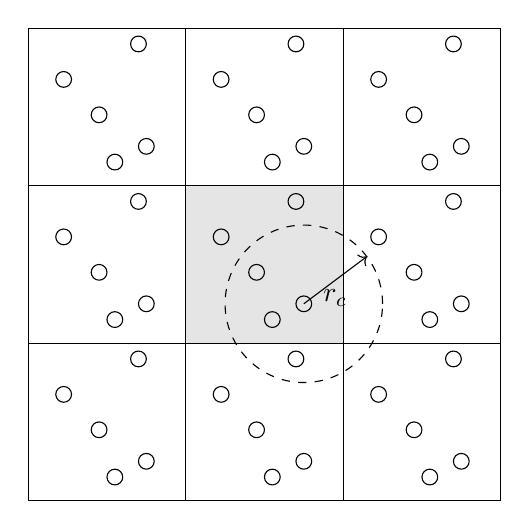
\begin{tikzpicture}
            \fill[gray!20] (0,0) rectangle (2,2);
            \foreach \i in {-2,0,2}{
                \foreach \j in {-2,0,2}{
                    \begin{scope}[shift={(\i,\j)}]
                        \draw (0,0) rectangle (2,2);
                        \draw (0.45,1.35) circle (0.1);
                        \draw (0.9,0.9) circle (0.1);
                        \draw (1.1,0.3) circle (0.1);
                        \draw (1.5,0.5) circle (0.1);
                        \draw (1.4,1.8) circle (0.1);
                    \end{scope}
                }
            }
            \draw[dashed] (1.5,0.5) circle (1);
            \draw[->] (1.5,0.5)--node[below]{\(r_c\)}(2.3,1.1);
        \end{tikzpicture}
        \caption{A simulation cell with cyclic boundary condition and cutoff radius \(r=r_c\).}
    \end{figure}

    \subsubsection{Pair Lists}
    When the cutoff radius \(r_c\) is much smaller than the cell dimensions, a lot of time will be spent checking whether a given pair of atoms is within the cutoff, when in fact most lie outside of it. In this case a useful time-saving measure is to use a ``pair list'' of atoms which are within \(r_c+\delta r\) of each other. Provided that this list is updated sufficiently often that no atom will have moved more than the buffer radius \(\delta r\) between updates, only this list of atom pairs needs to be checked at each time step, rather than all possible pairs.

    \subsubsection{Initialising Positions and Momenta}
    For most purposes, we want our simulation to get to equilibrium as fast as possible. You can either pre-arrange the particles on a regular lattice, or place them randomly within the simulation cell. However, putting particles randomly can sometimes lead to extreme coordinates (e.g. two molecules are too close to each other / overlapping), and so sometimes a short steepest-descent is required to remove those situations before the simulation has started.

    To set up the initial momenta, we can sample randomly from a Gaussian distribution
    \begin{equation}
        P(v)\propto \exp\left(-\frac{mv^2}{2k_B T}\right)
    \end{equation}
    for each component of a particle's velocity. However, these randomly generated velocities sometimes give a non-zero total momentum of the system, so we want to correct non-zero velocities of the centre of mass:
    \begin{align}
        \vb{v}_{\text{CoM}}&=\frac{1}{M}\sum_i m_i\vb{v}_i \\
        \vb{v}_i'&=\vb{v}_i-\vb{v}_{\text{CoM}}\,.
    \end{align}
    Moreover, the randomly generated velocity may deviate from our desired temperature (recall the equipartition theorem), so we need to rescale the velocity by a factor of \(\sqrt{T_{\text{target}}/T_{\text{sample}}}\) to reach the desired temperature.

    \subsubsection{Time Steps}
    A good choice of time step is a balance between accuracy and computational cost. Too large a time step will lead to large errors in numerical integration. The time step should be significantly smaller than the time scale \(\tau\) associated with the fastest-frequency oscillation in the system: a step of size \(\tau/20\) is usually safe for Verlet-based schemes. The best indication for the breakdown of accuracy in the Verlet scheme due to too large time steps is the drift of total energy, which should be rigorously conserved according to Newton's equation of motion.

    \begin{figure}
        \centering
        % This file was created with tikzplotlib v0.10.1.
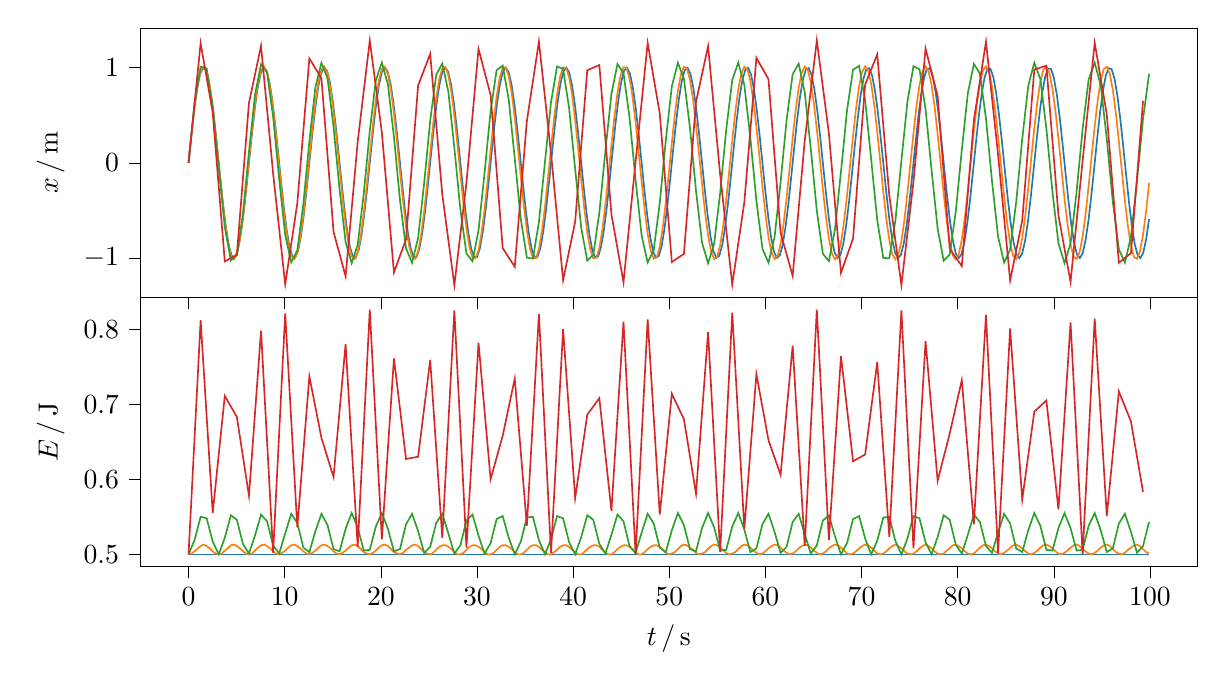
\begin{tikzpicture}

\definecolor{crimson2143940}{RGB}{214,39,40}
\definecolor{darkgray176}{RGB}{176,176,176}
\definecolor{darkorange25512714}{RGB}{255,127,14}
\definecolor{forestgreen4416044}{RGB}{44,160,44}
\definecolor{steelblue31119180}{RGB}{31,119,180}

\begin{groupplot}[group style={group size=1 by 2,vertical sep=0pt,xticklabels at=edge bottom},height=5cm,width=15cm]
\nextgroupplot[
scaled x ticks=manual:{}{\pgfmathparse{#1}},
tick align=outside,
tick pos=left,
x grid style={darkgray176},
xmin=-4.99515, xmax=104.89815,
xtick style={color=black},
xticklabels={},
y grid style={darkgray176},
ylabel={\(\displaystyle x\,/\,\mathrm{m}\)},
ymin=-1.41234, ymax=1.41334,
ytick style={color=black}
]
\addplot [semithick, steelblue31119180]
table {%
0 0
0.3 0.296
0.6 0.565
0.9 0.783
1.2 0.932
1.5 0.997
1.8 0.974
2.1 0.863
2.4 0.675
2.7 0.427
3 0.141
3.3 -0.158
3.6 -0.443
3.9 -0.688
4.2 -0.872
4.5 -0.978
4.8 -0.996
5.1 -0.926
5.4 -0.773
5.7 -0.551
6 -0.279
6.3 0.017
6.6 0.312
6.9 0.578
7.2 0.794
7.5 0.938
7.8 0.999
8.1 0.97
8.4 0.855
8.7 0.663
9 0.412
9.3 0.124
9.6 -0.174
9.9 -0.458
10.2 -0.7
10.5 -0.88
10.8 -0.981
11.1 -0.995
11.4 -0.919
11.7 -0.762
12 -0.537
12.3 -0.263
12.6 0.034
12.9 0.327
13.2 0.592
13.5 0.804
13.8 0.944
14.1 0.999
14.4 0.966
14.7 0.846
15 0.65
15.3 0.397
15.6 0.108
15.9 -0.191
16.2 -0.472
16.5 -0.712
16.8 -0.888
17.1 -0.984
17.4 -0.993
17.7 -0.913
18 -0.751
18.3 -0.522
18.6 -0.247
18.9 0.05
19.2 0.343
19.5 0.606
19.8 0.814
20.1 0.949
20.4 1
20.7 0.961
21 0.837
21.3 0.637
21.6 0.381
21.9 0.091
22.2 -0.207
22.5 -0.487
22.8 -0.723
23.1 -0.895
23.4 -0.987
23.7 -0.99
24 -0.906
24.3 -0.74
24.6 -0.508
24.9 -0.231
25.2 0.067
25.5 0.359
25.8 0.619
26.1 0.823
26.4 0.954
26.7 1
27 0.956
27.3 0.827
27.6 0.624
27.9 0.366
28.2 0.074
28.5 -0.224
28.8 -0.502
29.1 -0.735
29.4 -0.903
29.7 -0.989
30 -0.988
30.3 -0.898
30.6 -0.728
30.9 -0.493
31.2 -0.214
31.5 0.084
31.8 0.375
32.1 0.632
32.4 0.833
32.7 0.959
33 1
33.3 0.951
33.6 0.818
33.9 0.611
34.2 0.35
34.5 0.057
34.8 -0.24
35.1 -0.516
35.4 -0.746
35.7 -0.91
36 -0.992
36.3 -0.985
36.6 -0.891
36.9 -0.717
37.2 -0.479
37.5 -0.198
37.8 0.101
38.1 0.39
38.4 0.645
38.7 0.842
39 0.964
39.3 1
39.6 0.946
39.9 0.808
40.2 0.598
40.5 0.334
40.8 0.041
41.1 -0.256
41.4 -0.531
41.7 -0.757
42 -0.917
42.3 -0.994
42.6 -0.982
42.9 -0.883
43.2 -0.705
43.5 -0.464
43.8 -0.181
44.1 0.117
44.4 0.406
44.7 0.658
45 0.851
45.3 0.968
45.6 0.999
45.9 0.94
46.2 0.798
46.5 0.584
46.8 0.318
47.1 0.024
47.4 -0.273
47.7 -0.545
48 -0.768
48.3 -0.923
48.6 -0.996
48.9 -0.979
49.2 -0.875
49.5 -0.693
49.8 -0.449
50.1 -0.165
50.4 0.134
50.7 0.421
51 0.67
51.3 0.86
51.6 0.972
51.9 0.998
52.2 0.935
52.5 0.788
52.8 0.57
53.1 0.302
53.4 0.007
53.7 -0.289
54 -0.559
54.3 -0.779
54.6 -0.929
54.9 -0.997
55.2 -0.975
55.5 -0.867
55.8 -0.681
56.1 -0.434
56.4 -0.148
56.7 0.151
57 0.436
57.3 0.683
57.6 0.868
57.9 0.976
58.2 0.997
58.5 0.928
58.8 0.777
59.1 0.557
59.4 0.286
59.7 -0.01
60 -0.305
60.3 -0.573
60.6 -0.789
60.9 -0.936
61.2 -0.998
61.5 -0.972
61.8 -0.858
62.1 -0.668
62.4 -0.419
62.7 -0.131
63 0.167
63.3 0.451
63.6 0.695
63.9 0.876
64.2 0.98
64.5 0.995
64.8 0.922
65.1 0.767
65.4 0.543
65.7 0.27
66 -0.027
66.3 -0.321
66.6 -0.586
66.9 -0.8
67.2 -0.941
67.5 -0.999
67.8 -0.967
68.1 -0.85
68.4 -0.656
68.7 -0.403
69 -0.115
69.3 0.184
69.6 0.466
69.9 0.707
70.2 0.884
70.5 0.983
70.8 0.993
71.1 0.915
71.4 0.756
71.7 0.528
72 0.254
72.3 -0.043
72.6 -0.337
72.9 -0.6
73.2 -0.81
73.5 -0.947
73.8 -1
74.1 -0.963
74.4 -0.841
74.7 -0.643
75 -0.388
75.3 -0.098
75.6 0.2
75.9 0.481
76.2 0.719
76.5 0.892
76.8 0.986
77.1 0.991
77.4 0.909
77.7 0.745
78 0.514
78.3 0.238
78.6 -0.06
78.9 -0.352
79.2 -0.613
79.5 -0.819
79.8 -0.952
80.1 -1
80.4 -0.958
80.7 -0.831
81 -0.63
81.3 -0.372
81.6 -0.081
81.9 0.217
82.2 0.496
82.5 0.73
82.8 0.899
83.1 0.988
83.4 0.989
83.7 0.901
84 0.733
84.3 0.499
84.6 0.221
84.9 -0.077
85.2 -0.368
85.5 -0.626
85.8 -0.829
86.1 -0.957
86.4 -1
86.7 -0.953
87 -0.822
87.3 -0.617
87.6 -0.357
87.9 -0.065
88.2 0.233
88.5 0.51
88.8 0.742
89.1 0.907
89.4 0.991
89.7 0.986
90 0.894
90.3 0.722
90.6 0.485
90.9 0.205
91.2 -0.094
91.5 -0.384
91.8 -0.639
92.1 -0.838
92.4 -0.962
92.7 -1
93 -0.948
93.3 -0.812
93.6 -0.603
93.9 -0.341
94.2 -0.048
94.5 0.25
94.8 0.525
95.1 0.753
95.4 0.914
95.7 0.993
96 0.984
96.3 0.886
96.6 0.71
96.9 0.47
97.2 0.188
97.5 -0.11
97.8 -0.399
98.1 -0.652
98.4 -0.847
98.7 -0.966
99 -0.999
99.3 -0.943
99.6 -0.802
99.9 -0.59
};
\addplot [semithick, darkorange25512714]
table {%
0 0
0.314 0.3142
0.628 0.5973
0.942 0.8215
1.257 0.9646
1.571 1.0125
1.885 0.9605
2.199 0.8137
2.513 0.5866
2.827 0.3016
3.142 -0.0132
3.456 -0.3267
3.77 -0.6079
4.084 -0.8292
4.398 -0.9686
4.712 -1.0124
5.027 -0.9563
5.341 -0.8058
5.655 -0.5757
5.969 -0.2889
6.283 0.0265
6.597 0.3392
6.912 0.6185
7.226 0.8367
7.54 0.9723
7.854 1.012
8.168 0.9518
8.482 0.7977
8.796 0.5648
9.111 0.2762
9.425 -0.0397
9.739 -0.3516
10.053 -0.6289
10.367 -0.8441
10.681 -0.976
10.996 -1.0115
11.31 -0.9472
11.624 -0.7895
11.938 -0.5538
12.252 -0.2634
12.566 0.0529
12.881 0.364
13.195 0.6392
13.509 0.8513
13.823 0.9794
14.137 1.0108
14.451 0.9425
14.765 0.7811
15.08 0.5427
15.394 0.2507
15.708 -0.0661
16.022 -0.3763
16.336 -0.6494
16.65 -0.8584
16.965 -0.9827
17.279 -1.01
17.593 -0.9376
17.907 -0.7726
18.221 -0.5315
18.535 -0.2378
18.85 0.0793
19.164 0.3886
19.478 0.6595
19.792 0.8653
20.106 0.9858
20.42 1.0089
20.735 0.9325
21.049 0.764
21.363 0.5201
21.677 0.2249
21.991 -0.0925
22.305 -0.4008
22.619 -0.6695
22.934 -0.8721
23.248 -0.9887
23.562 -1.0077
23.876 -0.9273
24.19 -0.7553
24.504 -0.5088
24.819 -0.212
25.133 0.1056
25.447 0.4129
25.761 0.6794
26.075 0.8788
26.389 0.9915
26.704 1.0063
27.018 0.9219
27.332 0.7464
27.646 0.4973
27.96 0.1991
28.274 -0.1188
28.588 -0.4249
28.903 -0.6891
29.217 -0.8853
29.531 -0.9941
29.845 -1.0048
30.159 -0.9163
30.473 -0.7374
30.788 -0.4857
31.102 -0.1861
31.416 0.1319
31.73 0.4369
32.044 0.6987
32.358 0.8916
32.673 0.9965
32.987 1.0031
33.301 0.9106
33.615 0.7283
33.929 0.4741
34.243 0.1731
34.558 -0.145
34.872 -0.4488
35.186 -0.7083
35.5 -0.8978
35.814 -0.9988
36.128 -1.0012
36.442 -0.9047
36.757 -0.719
37.071 -0.4623
37.385 -0.16
37.699 0.1581
38.013 0.4606
38.327 0.7176
38.642 0.9039
38.956 1.0009
39.27 0.9991
39.584 0.8987
39.898 0.7096
40.212 0.4505
40.527 0.1469
40.841 -0.1712
41.155 -0.4723
41.469 -0.7269
41.783 -0.9097
42.097 -1.0028
42.412 -0.9969
42.726 -0.8925
43.04 -0.7001
43.354 -0.4386
43.668 -0.1338
43.982 0.1842
44.296 0.484
44.611 0.7361
44.925 0.9155
45.239 1.0045
45.553 0.9945
45.867 0.8862
46.181 0.6905
46.496 0.4267
46.81 0.1207
47.124 -0.1972
47.438 -0.4956
47.752 -0.7451
48.066 -0.9211
48.381 -1.0061
48.695 -0.9919
49.009 -0.8797
49.323 -0.6808
49.637 -0.4146
49.951 -0.1076
50.265 0.2101
50.58 0.5071
50.894 0.754
51.208 0.9265
51.522 1.0075
51.836 0.9891
52.15 0.8731
52.465 0.6709
52.779 0.4025
53.093 0.0944
53.407 -0.2231
53.721 -0.5185
54.035 -0.7627
54.35 -0.9317
54.664 -1.0088
54.978 -0.9862
55.292 -0.8663
55.606 -0.661
55.92 -0.3904
56.235 -0.0812
56.549 0.2359
56.863 0.5298
57.177 0.7714
57.491 0.9368
57.805 1.0098
58.119 0.9831
58.434 0.8594
58.748 0.6509
59.062 0.3781
59.376 0.068
59.69 -0.2488
60.004 -0.541
60.319 -0.7799
60.633 -0.9418
60.947 -1.0107
61.261 -0.9799
61.575 -0.8524
61.889 -0.6407
62.204 -0.3658
62.518 -0.0548
62.832 0.2616
63.146 0.5522
63.46 0.7883
63.774 0.9466
64.088 1.0114
64.403 0.9765
64.717 0.8451
65.031 0.6304
65.345 0.3534
65.659 0.0416
65.973 -0.2743
66.288 -0.5632
66.602 -0.7965
66.916 -0.9512
67.23 -1.012
67.544 -0.9729
67.858 -0.8378
68.173 -0.62
68.487 -0.341
68.801 -0.0284
69.115 0.287
69.429 0.5742
69.743 0.8046
70.058 0.9556
70.372 1.0123
70.686 0.9691
71 0.8303
71.314 0.6095
71.628 0.3285
71.942 0.0152
72.257 -0.2997
72.571 -0.585
72.885 -0.8126
73.199 -0.9599
73.513 -1.0125
73.827 -0.9652
74.142 -0.8226
74.456 -0.5989
74.77 -0.316
75.084 -0.0019
75.398 0.3123
75.712 0.5958
76.027 0.8204
76.341 0.964
76.655 1.0126
76.969 0.9611
77.283 0.8149
77.597 0.5882
77.911 0.3034
78.226 -0.0113
78.54 -0.3249
78.854 -0.6064
79.168 -0.8281
79.482 -0.968
79.796 -1.0124
80.111 -0.9569
80.425 -0.8069
80.739 -0.5773
81.053 -0.2908
81.367 0.0245
81.681 0.3374
81.996 0.6169
82.31 0.8356
82.624 0.9718
82.938 1.0121
83.252 0.9525
83.566 0.7989
83.881 0.5664
84.195 0.2781
84.509 -0.0377
84.823 -0.3498
85.137 -0.6274
85.451 -0.843
85.765 -0.9754
86.08 -1.0116
86.394 -0.9479
86.708 -0.7907
87.022 -0.5554
87.336 -0.2653
87.65 0.051
87.965 0.3622
88.279 0.6377
88.593 0.8503
88.907 0.9789
89.221 1.0109
89.535 0.9432
89.85 0.7823
90.164 0.5443
90.478 0.2525
90.792 -0.0642
91.106 -0.3745
91.42 -0.6479
91.735 -0.8574
92.049 -0.9822
92.363 -1.0101
92.677 -0.9383
92.991 -0.7739
93.305 -0.5331
93.619 -0.2397
93.934 0.0774
94.248 0.3868
94.562 0.658
94.876 0.8643
95.19 0.9853
95.504 1.0091
95.819 0.9332
96.133 0.7653
96.447 0.5218
96.761 0.2268
97.075 -0.0905
97.389 -0.399
97.704 -0.668
98.018 -0.8712
98.332 -0.9883
98.646 -1.0079
98.96 -0.928
99.274 -0.7566
99.588 -0.5104
99.903 -0.2139
};
\addplot [semithick, forestgreen4416044]
table {%
0 0
0.628 0.6283
1.257 1.0086
1.885 0.9907
2.513 0.5817
3.142 -0.057
3.77 -0.6731
4.398 -1.0235
5.027 -0.9699
5.655 -0.5333
6.283 0.1138
6.912 0.716
7.54 1.0355
8.168 0.9462
8.796 0.4834
9.425 -0.1703
10.053 -0.7567
10.681 -1.0444
11.31 -0.9198
11.938 -0.4321
12.566 0.2262
13.195 0.7952
13.823 1.0503
14.451 0.8907
15.08 0.3795
15.708 -0.2815
16.336 -0.8314
16.965 -1.0531
17.593 -0.859
18.221 -0.3258
18.85 0.336
19.478 0.8652
20.106 1.0528
20.735 0.8248
21.363 0.2711
21.991 -0.3895
22.619 -0.8964
23.248 -1.0494
23.876 -0.7881
24.504 -0.2157
25.133 0.4419
25.761 0.925
26.389 1.043
27.018 0.7491
27.646 0.1596
28.274 -0.493
28.903 -0.9509
29.531 -1.0335
30.159 -0.708
30.788 -0.103
31.416 0.5426
32.044 0.974
32.673 1.0209
33.301 0.6648
33.929 0.0462
34.558 -0.5906
35.186 -0.9943
35.814 -1.0054
36.442 -0.6196
37.071 0.0108
37.699 0.637
38.327 1.0117
38.956 0.987
39.584 0.5726
40.212 -0.0678
40.841 -0.6814
41.469 -1.026
42.097 -0.9656
42.726 -0.524
43.354 0.1245
43.982 0.7239
44.611 1.0374
45.239 0.9414
45.867 0.4738
46.496 -0.1809
47.124 -0.7642
47.752 -1.0458
48.381 -0.9145
49.009 -0.4222
49.637 0.2368
50.265 0.8023
50.894 1.0511
51.522 0.8849
52.15 0.3694
52.779 -0.2919
53.407 -0.838
54.035 -1.0533
54.664 -0.8527
55.292 -0.3155
55.92 0.3463
56.549 0.8713
57.177 1.0524
57.805 0.818
58.434 0.2607
59.062 -0.3996
59.69 -0.9021
60.319 -1.0484
60.947 -0.7809
61.575 -0.2051
62.204 0.4517
62.832 0.9302
63.46 1.0414
64.088 0.7415
64.717 0.1489
65.345 -0.5025
65.973 -0.9555
66.602 -1.0313
67.23 -0.7
67.858 -0.0923
68.487 0.5518
69.115 0.9781
69.743 1.0182
70.372 0.6564
71 0.0354
71.628 -0.5996
72.257 -0.9978
72.885 -1.0021
73.513 -0.6108
74.142 0.0216
74.77 0.6455
75.398 1.0146
76.027 0.9831
76.655 0.5635
77.283 -0.0785
77.911 -0.6896
78.54 -1.0284
79.168 -0.9612
79.796 -0.5146
80.425 0.1352
81.053 0.7317
81.681 1.0392
82.31 0.9365
82.938 0.4641
83.566 -0.1916
84.195 -0.7716
84.823 -1.047
85.451 -0.9091
86.08 -0.4123
86.708 0.2473
87.336 0.8092
87.965 1.0517
88.593 0.879
89.221 0.3592
89.85 -0.3023
90.478 -0.8445
91.106 -1.0533
91.735 -0.8463
92.363 -0.3052
92.991 0.3565
93.619 0.8773
94.248 1.0519
94.876 0.8111
95.504 0.2502
96.133 -0.4095
96.761 -0.9076
97.389 -1.0473
98.018 -0.7736
98.646 -0.1945
99.274 0.4614
99.903 0.9352
};
\addplot [semithick, crimson2143940]
table {%
0 0
1.257 1.2566
2.513 0.5289
3.77 -1.0341
5.027 -0.9641
6.283 0.6283
7.54 1.2285
8.796 -0.1113
10.053 -1.2753
11.31 -0.4255
12.566 1.0963
13.823 0.8868
15.08 -0.723
16.336 -1.1911
17.593 0.2217
18.85 1.2845
20.106 0.3189
21.363 -1.1503
22.619 -0.803
23.876 0.8123
25.133 1.1448
26.389 -0.3305
27.646 -1.2839
28.903 -0.2099
30.159 1.1956
31.416 0.713
32.673 -0.8955
33.929 -1.0899
35.186 0.4368
36.442 1.2738
37.699 0.0993
38.956 -1.232
40.212 -0.6178
41.469 0.972
42.726 1.0269
43.982 -0.5398
45.239 -1.254
46.496 0.012
47.752 1.2591
49.009 0.5179
50.265 -1.0412
51.522 -0.9561
52.779 0.6388
54.035 1.2249
55.292 -0.1233
56.549 -1.2768
57.805 -0.4141
59.062 1.1025
60.319 0.8781
61.575 -0.733
62.832 -1.1866
64.088 0.2336
65.345 1.2849
66.602 0.3072
67.858 -1.1556
69.115 -0.7935
70.372 0.8216
71.628 1.1393
72.885 -0.3421
74.142 -1.2833
75.398 -0.198
76.655 1.2
77.911 0.703
79.168 -0.9041
80.425 -1.0835
81.681 0.4481
82.938 1.2721
84.195 0.0873
85.451 -1.2354
86.708 -0.6072
87.965 0.9798
89.221 1.0196
90.478 -0.5507
91.735 -1.2513
92.991 0.0241
94.248 1.2615
95.504 0.5068
96.761 -1.0482
98.018 -0.948
99.274 0.6492
};

\nextgroupplot[
tick align=outside,
tick pos=left,
x grid style={darkgray176},
xlabel={\(\displaystyle t\,/\,\mathrm{s}\)},
xmin=-4.99515, xmax=104.89815,
xtick style={color=black},
y grid style={darkgray176},
ylabel={\(\displaystyle E\,/\,\mathrm{J}\)},
ymin=0.4837, ymax=0.8423,
ytick style={color=black}
]
\addplot [semithick, steelblue31119180]
table {%
0 0.5
0.3 0.5
0.6 0.5
0.9 0.5
1.2 0.5
1.5 0.5
1.8 0.5
2.1 0.5
2.4 0.5
2.7 0.5
3 0.5
3.3 0.5
3.6 0.5
3.9 0.5
4.2 0.5
4.5 0.5
4.8 0.5
5.1 0.5
5.4 0.5
5.7 0.5
6 0.5
6.3 0.5
6.6 0.5
6.9 0.5
7.2 0.5
7.5 0.5
7.8 0.5
8.1 0.5
8.4 0.5
8.7 0.5
9 0.5
9.3 0.5
9.6 0.5
9.9 0.5
10.2 0.5
10.5 0.5
10.8 0.5
11.1 0.5
11.4 0.5
11.7 0.5
12 0.5
12.3 0.5
12.6 0.5
12.9 0.5
13.2 0.5
13.5 0.5
13.8 0.5
14.1 0.5
14.4 0.5
14.7 0.5
15 0.5
15.3 0.5
15.6 0.5
15.9 0.5
16.2 0.5
16.5 0.5
16.8 0.5
17.1 0.5
17.4 0.5
17.7 0.5
18 0.5
18.3 0.5
18.6 0.5
18.9 0.5
19.2 0.5
19.5 0.5
19.8 0.5
20.1 0.5
20.4 0.5
20.7 0.5
21 0.5
21.3 0.5
21.6 0.5
21.9 0.5
22.2 0.5
22.5 0.5
22.8 0.5
23.1 0.5
23.4 0.5
23.7 0.5
24 0.5
24.3 0.5
24.6 0.5
24.9 0.5
25.2 0.5
25.5 0.5
25.8 0.5
26.1 0.5
26.4 0.5
26.7 0.5
27 0.5
27.3 0.5
27.6 0.5
27.9 0.5
28.2 0.5
28.5 0.5
28.8 0.5
29.1 0.5
29.4 0.5
29.7 0.5
30 0.5
30.3 0.5
30.6 0.5
30.9 0.5
31.2 0.5
31.5 0.5
31.8 0.5
32.1 0.5
32.4 0.5
32.7 0.5
33 0.5
33.3 0.5
33.6 0.5
33.9 0.5
34.2 0.5
34.5 0.5
34.8 0.5
35.1 0.5
35.4 0.5
35.7 0.5
36 0.5
36.3 0.5
36.6 0.5
36.9 0.5
37.2 0.5
37.5 0.5
37.8 0.5
38.1 0.5
38.4 0.5
38.7 0.5
39 0.5
39.3 0.5
39.6 0.5
39.9 0.5
40.2 0.5
40.5 0.5
40.8 0.5
41.1 0.5
41.4 0.5
41.7 0.5
42 0.5
42.3 0.5
42.6 0.5
42.9 0.5
43.2 0.5
43.5 0.5
43.8 0.5
44.1 0.5
44.4 0.5
44.7 0.5
45 0.5
45.3 0.5
45.6 0.5
45.9 0.5
46.2 0.5
46.5 0.5
46.8 0.5
47.1 0.5
47.4 0.5
47.7 0.5
48 0.5
48.3 0.5
48.6 0.5
48.9 0.5
49.2 0.5
49.5 0.5
49.8 0.5
50.1 0.5
50.4 0.5
50.7 0.5
51 0.5
51.3 0.5
51.6 0.5
51.9 0.5
52.2 0.5
52.5 0.5
52.8 0.5
53.1 0.5
53.4 0.5
53.7 0.5
54 0.5
54.3 0.5
54.6 0.5
54.9 0.5
55.2 0.5
55.5 0.5
55.8 0.5
56.1 0.5
56.4 0.5
56.7 0.5
57 0.5
57.3 0.5
57.6 0.5
57.9 0.5
58.2 0.5
58.5 0.5
58.8 0.5
59.1 0.5
59.4 0.5
59.7 0.5
60 0.5
60.3 0.5
60.6 0.5
60.9 0.5
61.2 0.5
61.5 0.5
61.8 0.5
62.1 0.5
62.4 0.5
62.7 0.5
63 0.5
63.3 0.5
63.6 0.5
63.9 0.5
64.2 0.5
64.5 0.5
64.8 0.5
65.1 0.5
65.4 0.5
65.7 0.5
66 0.5
66.3 0.5
66.6 0.5
66.9 0.5
67.2 0.5
67.5 0.5
67.8 0.5
68.1 0.5
68.4 0.5
68.7 0.5
69 0.5
69.3 0.5
69.6 0.5
69.9 0.5
70.2 0.5
70.5 0.5
70.8 0.5
71.1 0.5
71.4 0.5
71.7 0.5
72 0.5
72.3 0.5
72.6 0.5
72.9 0.5
73.2 0.5
73.5 0.5
73.8 0.5
74.1 0.5
74.4 0.5
74.7 0.5
75 0.5
75.3 0.5
75.6 0.5
75.9 0.5
76.2 0.5
76.5 0.5
76.8 0.5
77.1 0.5
77.4 0.5
77.7 0.5
78 0.5
78.3 0.5
78.6 0.5
78.9 0.5
79.2 0.5
79.5 0.5
79.8 0.5
80.1 0.5
80.4 0.5
80.7 0.5
81 0.5
81.3 0.5
81.6 0.5
81.9 0.5
82.2 0.5
82.5 0.5
82.8 0.5
83.1 0.5
83.4 0.5
83.7 0.5
84 0.5
84.3 0.5
84.6 0.5
84.9 0.5
85.2 0.5
85.5 0.5
85.8 0.5
86.1 0.5
86.4 0.5
86.7 0.5
87 0.5
87.3 0.5
87.6 0.5
87.9 0.5
88.2 0.5
88.5 0.5
88.8 0.5
89.1 0.5
89.4 0.5
89.7 0.5
90 0.5
90.3 0.5
90.6 0.5
90.9 0.5
91.2 0.5
91.5 0.5
91.8 0.5
92.1 0.5
92.4 0.5
92.7 0.5
93 0.5
93.3 0.5
93.6 0.5
93.9 0.5
94.2 0.5
94.5 0.5
94.8 0.5
95.1 0.5
95.4 0.5
95.7 0.5
96 0.5
96.3 0.5
96.6 0.5
96.9 0.5
97.2 0.5
97.5 0.5
97.8 0.5
98.1 0.5
98.4 0.5
98.7 0.5
99 0.5
99.3 0.5
99.6 0.5
99.9 0.5
};
\addplot [semithick, darkorange25512714]
table {%
0 0.5
0.314 0.501
0.628 0.504
0.942 0.508
1.257 0.511
1.571 0.513
1.885 0.511
2.199 0.508
2.513 0.504
2.827 0.501
3.142 0.5
3.456 0.501
3.77 0.505
4.084 0.508
4.398 0.512
4.712 0.513
5.027 0.511
5.341 0.508
5.655 0.504
5.969 0.501
6.283 0.5
6.597 0.501
6.912 0.505
7.226 0.509
7.54 0.512
7.854 0.513
8.168 0.511
8.482 0.508
8.796 0.504
9.111 0.501
9.425 0.5
9.739 0.502
10.053 0.505
10.367 0.509
10.681 0.512
10.996 0.513
11.31 0.511
11.624 0.508
11.938 0.504
12.252 0.501
12.566 0.5
12.881 0.502
13.195 0.505
13.509 0.509
13.823 0.512
14.137 0.513
14.451 0.511
14.765 0.508
15.08 0.504
15.394 0.501
15.708 0.5
16.022 0.502
16.336 0.505
16.65 0.509
16.965 0.512
17.279 0.513
17.593 0.511
17.907 0.507
18.221 0.503
18.535 0.501
18.85 0.5
19.164 0.502
19.478 0.505
19.792 0.509
20.106 0.512
20.42 0.513
20.735 0.511
21.049 0.507
21.363 0.503
21.677 0.501
21.991 0.5
22.305 0.502
22.619 0.506
22.934 0.509
23.248 0.512
23.562 0.513
23.876 0.511
24.19 0.507
24.504 0.503
24.819 0.501
25.133 0.5
25.447 0.502
25.761 0.506
26.075 0.51
26.389 0.512
26.704 0.512
27.018 0.51
27.332 0.507
27.646 0.503
27.96 0.5
28.274 0.5
28.588 0.502
28.903 0.506
29.217 0.51
29.531 0.512
29.845 0.512
30.159 0.51
30.473 0.507
30.788 0.503
31.102 0.5
31.416 0.5
31.73 0.502
32.044 0.506
32.358 0.51
32.673 0.512
32.987 0.512
33.301 0.51
33.615 0.507
33.929 0.503
34.243 0.5
34.558 0.5
34.872 0.502
35.186 0.506
35.5 0.51
35.814 0.512
36.128 0.512
36.442 0.51
36.757 0.506
37.071 0.503
37.385 0.5
37.699 0.5
38.013 0.503
38.327 0.506
38.642 0.51
38.956 0.512
39.27 0.512
39.584 0.51
39.898 0.506
40.212 0.503
40.527 0.5
40.841 0.5
41.155 0.503
41.469 0.507
41.783 0.51
42.097 0.512
42.412 0.512
42.726 0.51
43.04 0.506
43.354 0.502
43.668 0.5
43.982 0.5
44.296 0.503
44.611 0.507
44.925 0.51
45.239 0.512
45.553 0.512
45.867 0.51
46.181 0.506
46.496 0.502
46.81 0.5
47.124 0.5
47.438 0.503
47.752 0.507
48.066 0.51
48.381 0.512
48.695 0.512
49.009 0.51
49.323 0.506
49.637 0.502
49.951 0.5
50.265 0.501
50.58 0.503
50.894 0.507
51.208 0.511
51.522 0.513
51.836 0.512
52.15 0.509
52.465 0.506
52.779 0.502
53.093 0.5
53.407 0.501
53.721 0.503
54.035 0.507
54.35 0.511
54.664 0.513
54.978 0.512
55.292 0.509
55.606 0.505
55.92 0.502
56.235 0.5
56.549 0.501
56.863 0.503
57.177 0.507
57.491 0.511
57.805 0.513
58.119 0.512
58.434 0.509
58.748 0.505
59.062 0.502
59.376 0.5
59.69 0.501
60.004 0.504
60.319 0.508
60.633 0.511
60.947 0.513
61.261 0.512
61.575 0.509
61.889 0.505
62.204 0.502
62.518 0.5
62.832 0.501
63.146 0.504
63.46 0.508
63.774 0.511
64.088 0.513
64.403 0.512
64.717 0.509
65.031 0.505
65.345 0.502
65.659 0.5
65.973 0.501
66.288 0.504
66.602 0.508
66.916 0.511
67.23 0.513
67.544 0.512
67.858 0.509
68.173 0.505
68.487 0.501
68.801 0.5
69.115 0.501
69.429 0.504
69.743 0.508
70.058 0.511
70.372 0.513
70.686 0.512
71 0.509
71.314 0.505
71.628 0.501
71.942 0.5
72.257 0.501
72.571 0.504
72.885 0.508
73.199 0.511
73.513 0.513
73.827 0.511
74.142 0.508
74.456 0.504
74.77 0.501
75.084 0.5
75.398 0.501
75.712 0.504
76.027 0.508
76.341 0.511
76.655 0.513
76.969 0.511
77.283 0.508
77.597 0.504
77.911 0.501
78.226 0.5
78.54 0.501
78.854 0.505
79.168 0.508
79.482 0.512
79.796 0.513
80.111 0.511
80.425 0.508
80.739 0.504
81.053 0.501
81.367 0.5
81.681 0.501
81.996 0.505
82.31 0.509
82.624 0.512
82.938 0.513
83.252 0.511
83.566 0.508
83.881 0.504
84.195 0.501
84.509 0.5
84.823 0.502
85.137 0.505
85.451 0.509
85.765 0.512
86.08 0.513
86.394 0.511
86.708 0.508
87.022 0.504
87.336 0.501
87.65 0.5
87.965 0.502
88.279 0.505
88.593 0.509
88.907 0.512
89.221 0.513
89.535 0.511
89.85 0.508
90.164 0.504
90.478 0.501
90.792 0.5
91.106 0.502
91.42 0.505
91.735 0.509
92.049 0.512
92.363 0.513
92.677 0.511
92.991 0.507
93.305 0.504
93.619 0.501
93.934 0.5
94.248 0.502
94.562 0.505
94.876 0.509
95.19 0.512
95.504 0.513
95.819 0.511
96.133 0.507
96.447 0.503
96.761 0.501
97.075 0.5
97.389 0.502
97.704 0.506
98.018 0.509
98.332 0.512
98.646 0.513
98.96 0.511
99.274 0.507
99.588 0.503
99.903 0.501
};
\addplot [semithick, forestgreen4416044]
table {%
0 0.5
0.628 0.519
1.257 0.55
1.885 0.548
2.513 0.517
3.142 0.5
3.77 0.522
4.398 0.552
5.027 0.546
5.655 0.514
6.283 0.501
6.912 0.525
7.54 0.553
8.168 0.544
8.796 0.512
9.425 0.501
10.053 0.528
10.681 0.554
11.31 0.542
11.938 0.509
12.566 0.503
13.195 0.531
13.823 0.554
14.451 0.539
15.08 0.507
15.708 0.504
16.336 0.534
16.965 0.555
17.593 0.536
18.221 0.505
18.85 0.506
19.478 0.537
20.106 0.555
20.735 0.534
21.363 0.504
21.991 0.507
22.619 0.54
23.248 0.554
23.876 0.531
24.504 0.502
25.133 0.51
25.761 0.542
26.389 0.554
27.018 0.528
27.646 0.501
28.274 0.512
28.903 0.545
29.531 0.553
30.159 0.525
30.788 0.501
31.416 0.515
32.044 0.547
32.673 0.551
33.301 0.522
33.929 0.5
34.558 0.517
35.186 0.549
35.814 0.55
36.442 0.519
37.071 0.5
37.699 0.52
38.327 0.551
38.956 0.548
39.584 0.516
40.212 0.5
40.841 0.523
41.469 0.552
42.097 0.546
42.726 0.514
43.354 0.501
43.982 0.526
44.611 0.553
45.239 0.544
45.867 0.511
46.496 0.502
47.124 0.529
47.752 0.554
48.381 0.541
49.009 0.509
49.637 0.503
50.265 0.532
50.894 0.555
51.522 0.539
52.15 0.507
52.779 0.504
53.407 0.535
54.035 0.555
54.664 0.536
55.292 0.505
55.92 0.506
56.549 0.537
57.177 0.555
57.805 0.533
58.434 0.503
59.062 0.508
59.69 0.54
60.319 0.554
60.947 0.53
61.575 0.502
62.204 0.51
62.832 0.543
63.46 0.554
64.088 0.527
64.717 0.501
65.345 0.512
65.973 0.545
66.602 0.552
67.23 0.524
67.858 0.5
68.487 0.515
69.115 0.547
69.743 0.551
70.372 0.521
71 0.5
71.628 0.518
72.257 0.549
72.885 0.55
73.513 0.518
74.142 0.5
74.77 0.521
75.398 0.551
76.027 0.548
76.655 0.516
77.283 0.5
77.911 0.523
78.54 0.552
79.168 0.546
79.796 0.513
80.425 0.501
81.053 0.526
81.681 0.553
82.31 0.543
82.938 0.511
83.566 0.502
84.195 0.529
84.823 0.554
85.451 0.541
86.08 0.508
86.708 0.503
87.336 0.532
87.965 0.555
88.593 0.538
89.221 0.506
89.85 0.505
90.478 0.535
91.106 0.555
91.735 0.535
92.363 0.505
92.991 0.506
93.619 0.538
94.248 0.555
94.876 0.532
95.504 0.503
96.133 0.508
96.761 0.541
97.389 0.554
98.018 0.53
98.646 0.502
99.274 0.511
99.903 0.543
};
\addplot [semithick, crimson2143940]
table {%
0 0.5
1.257 0.812
2.513 0.555
3.77 0.711
5.027 0.683
6.283 0.578
7.54 0.798
8.796 0.502
10.053 0.821
11.31 0.536
12.566 0.737
13.823 0.655
15.08 0.603
16.336 0.78
17.593 0.51
18.85 0.826
20.106 0.52
21.363 0.761
22.619 0.627
23.876 0.63
25.133 0.759
26.389 0.522
27.646 0.825
28.903 0.509
30.159 0.782
31.416 0.6
32.673 0.658
33.929 0.734
35.186 0.538
36.442 0.82
37.699 0.502
38.956 0.8
40.212 0.575
41.469 0.686
42.726 0.708
43.982 0.558
45.239 0.81
46.496 0.5
47.752 0.813
49.009 0.553
50.265 0.714
51.522 0.68
52.779 0.581
54.035 0.796
55.292 0.503
56.549 0.822
57.805 0.534
59.062 0.74
60.319 0.652
61.575 0.606
62.832 0.778
64.088 0.511
65.345 0.826
66.602 0.519
67.858 0.764
69.115 0.624
70.372 0.633
71.628 0.756
72.885 0.523
74.142 0.825
75.398 0.508
76.655 0.784
77.911 0.598
79.168 0.661
80.425 0.732
81.681 0.54
82.938 0.819
84.195 0.502
85.451 0.801
86.708 0.573
87.965 0.69
89.221 0.705
90.478 0.56
91.735 0.809
92.991 0.5
94.248 0.814
95.504 0.551
96.761 0.717
98.018 0.677
99.274 0.583
};
\end{groupplot}

\end{tikzpicture}

        \caption{Displacement and energy of a harmonic oscillator using Verlet algorithm with time steps \(\delta t=\tau/20\) (orange), \(\tau/10\) (green) and \(\tau/5\) (red) with exact results (blue).}
    \end{figure}
    \begin{figure}
        \centering
        % This file was created with tikzplotlib v0.10.1.
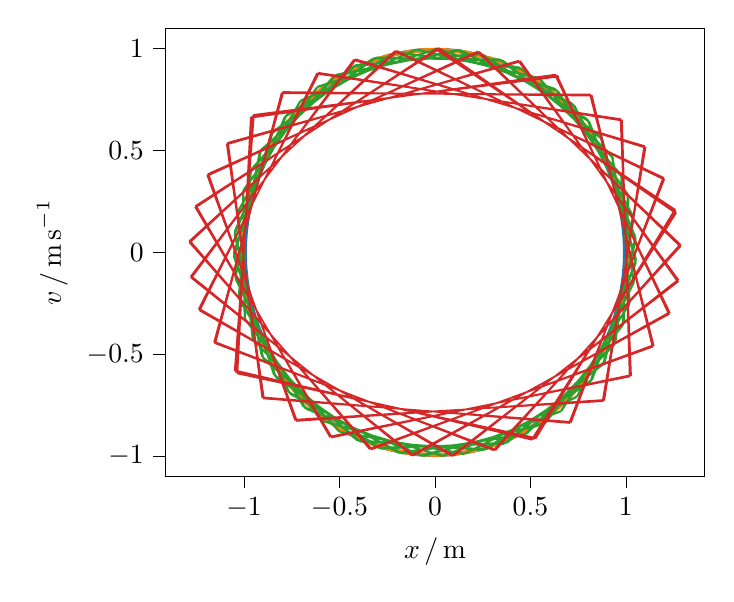
\begin{tikzpicture}

\definecolor{crimson2143940}{RGB}{214,39,40}
\definecolor{darkgray176}{RGB}{176,176,176}
\definecolor{darkorange25512714}{RGB}{255,127,14}
\definecolor{forestgreen4416044}{RGB}{44,160,44}
\definecolor{steelblue31119180}{RGB}{31,119,180}

\begin{axis}[
tick align=outside,
tick pos=left,
x grid style={darkgray176},
xlabel={\(\displaystyle x\,/\,\mathrm{m}\)},
xmin=-1.41234, xmax=1.41334,
xtick style={color=black},
y grid style={darkgray176},
ylabel={\(\displaystyle v\,/\,\mathrm{m\, s^{-1}}\)},
ymin=-1.1, ymax=1.1,
ytick style={color=black}
]
\addplot [semithick, steelblue31119180]
table {%
0 1
0.296 0.955
0.565 0.825
0.783 0.622
0.932 0.362
0.997 0.071
0.974 -0.227
0.863 -0.505
0.675 -0.737
0.427 -0.904
0.141 -0.99
-0.158 -0.987
-0.443 -0.897
-0.688 -0.726
-0.872 -0.49
-0.978 -0.211
-0.996 0.087
-0.926 0.378
-0.773 0.635
-0.551 0.835
-0.279 0.96
0.017 1
0.312 0.95
0.578 0.816
0.794 0.608
0.938 0.347
0.999 0.054
0.97 -0.244
0.855 -0.519
0.663 -0.749
0.412 -0.911
0.124 -0.992
-0.174 -0.985
-0.458 -0.889
-0.7 -0.714
-0.88 -0.476
-0.981 -0.194
-0.995 0.104
-0.919 0.393
-0.762 0.648
-0.537 0.844
-0.263 0.965
0.034 0.999
0.327 0.945
0.592 0.806
0.804 0.595
0.944 0.331
0.999 0.037
0.966 -0.26
0.846 -0.534
0.65 -0.76
0.397 -0.918
0.108 -0.994
-0.191 -0.982
-0.472 -0.881
-0.712 -0.702
-0.888 -0.461
-0.984 -0.178
-0.993 0.121
-0.913 0.409
-0.751 0.66
-0.522 0.853
-0.247 0.969
0.05 0.999
0.343 0.939
0.606 0.796
0.814 0.581
0.949 0.315
1 0.02
0.961 -0.276
0.837 -0.548
0.637 -0.771
0.381 -0.924
0.091 -0.996
-0.207 -0.978
-0.487 -0.873
-0.723 -0.69
-0.895 -0.446
-0.987 -0.161
-0.99 0.138
-0.906 0.424
-0.74 0.673
-0.508 0.861
-0.231 0.973
0.067 0.998
0.359 0.933
0.619 0.786
0.823 0.568
0.954 0.299
1 0.004
0.956 -0.292
0.827 -0.562
0.624 -0.781
0.366 -0.931
0.074 -0.997
-0.224 -0.975
-0.502 -0.865
-0.735 -0.678
-0.903 -0.431
-0.989 -0.145
-0.988 0.154
-0.898 0.439
-0.728 0.685
-0.493 0.87
-0.214 0.977
0.084 0.996
0.375 0.927
0.632 0.775
0.833 0.554
0.959 0.283
1 -0.013
0.951 -0.308
0.818 -0.576
0.611 -0.792
0.35 -0.937
0.057 -0.998
-0.24 -0.971
-0.516 -0.856
-0.746 -0.666
-0.91 -0.415
-0.992 -0.128
-0.985 0.171
-0.891 0.454
-0.717 0.697
-0.479 0.878
-0.198 0.98
0.101 0.995
0.39 0.921
0.645 0.764
0.842 0.54
0.964 0.267
1 -0.03
0.946 -0.324
0.808 -0.589
0.598 -0.802
0.334 -0.943
0.041 -0.999
-0.256 -0.967
-0.531 -0.848
-0.757 -0.653
-0.917 -0.4
-0.994 -0.111
-0.982 0.187
-0.883 0.469
-0.705 0.709
-0.464 0.886
-0.181 0.983
0.117 0.993
0.406 0.914
0.658 0.753
0.851 0.525
0.968 0.25
0.999 -0.047
0.94 -0.34
0.798 -0.603
0.584 -0.812
0.318 -0.948
0.024 -1
-0.273 -0.962
-0.545 -0.839
-0.768 -0.64
-0.923 -0.385
-0.996 -0.095
-0.979 0.204
-0.875 0.484
-0.693 0.721
-0.449 0.894
-0.165 0.986
0.134 0.991
0.421 0.907
0.67 0.742
0.86 0.511
0.972 0.234
0.998 -0.064
0.935 -0.356
0.788 -0.616
0.57 -0.821
0.302 -0.953
0.007 -1
-0.289 -0.957
-0.559 -0.829
-0.779 -0.627
-0.929 -0.369
-0.997 -0.078
-0.975 0.22
-0.867 0.499
-0.681 0.733
-0.434 0.901
-0.148 0.989
0.151 0.989
0.436 0.9
0.683 0.731
0.868 0.496
0.976 0.218
0.997 -0.08
0.928 -0.371
0.777 -0.629
0.557 -0.831
0.286 -0.958
-0.01 -1
-0.305 -0.952
-0.573 -0.82
-0.789 -0.614
-0.936 -0.353
-0.998 -0.061
-0.972 0.237
-0.858 0.513
-0.668 0.744
-0.419 0.908
-0.131 0.991
0.167 0.986
0.451 0.892
0.695 0.719
0.876 0.482
0.98 0.201
0.995 -0.097
0.922 -0.387
0.767 -0.642
0.543 -0.84
0.27 -0.963
-0.027 -1
-0.321 -0.947
-0.586 -0.81
-0.8 -0.601
-0.941 -0.337
-0.999 -0.044
-0.967 0.253
-0.85 0.528
-0.656 0.755
-0.403 0.915
-0.115 0.993
0.184 0.983
0.466 0.885
0.707 0.707
0.884 0.467
0.983 0.185
0.993 -0.114
0.915 -0.402
0.756 -0.655
0.528 -0.849
0.254 -0.967
-0.043 -0.999
-0.337 -0.942
-0.6 -0.8
-0.81 -0.587
-0.947 -0.322
-1 -0.027
-0.963 0.269
-0.841 0.542
-0.643 0.766
-0.388 0.922
-0.098 0.995
0.2 0.98
0.481 0.877
0.719 0.695
0.892 0.452
0.986 0.168
0.991 -0.131
0.909 -0.418
0.745 -0.668
0.514 -0.858
0.238 -0.971
-0.06 -0.998
-0.352 -0.936
-0.613 -0.79
-0.819 -0.573
-0.952 -0.306
-1 -0.011
-0.958 0.285
-0.831 0.556
-0.63 0.777
-0.372 0.928
-0.081 0.997
0.217 0.976
0.496 0.869
0.73 0.683
0.899 0.437
0.988 0.152
0.989 -0.147
0.901 -0.433
0.733 -0.68
0.499 -0.866
0.221 -0.975
-0.077 -0.997
-0.368 -0.93
-0.626 -0.779
-0.829 -0.56
-0.957 -0.29
-1 0.006
-0.953 0.301
-0.822 0.57
-0.617 0.787
-0.357 0.934
-0.065 0.998
0.233 0.972
0.51 0.86
0.742 0.671
0.907 0.422
0.991 0.135
0.986 -0.164
0.894 -0.448
0.722 -0.692
0.485 -0.875
0.205 -0.979
-0.094 -0.996
-0.384 -0.923
-0.639 -0.769
-0.838 -0.545
-0.962 -0.273
-1 0.023
-0.948 0.317
-0.812 0.583
-0.603 0.797
-0.341 0.94
-0.048 0.999
0.25 0.968
0.525 0.851
0.753 0.658
0.914 0.406
0.993 0.118
0.984 -0.18
0.886 -0.463
0.71 -0.704
0.47 -0.883
0.188 -0.982
-0.11 -0.994
-0.399 -0.917
-0.652 -0.758
-0.847 -0.531
-0.966 -0.257
-0.999 0.04
-0.943 0.333
-0.802 0.597
-0.59 0.807
};
\addplot [semithick, darkorange25512714]
table {%
0 1
0.3142 0.951
0.5973 0.807
0.8215 0.585
0.9646 0.304
1.0125 -0.007
0.9605 -0.316
0.8137 -0.595
0.5866 -0.815
0.3016 -0.955
-0.0132 -1
-0.3267 -0.947
-0.6079 -0.8
-0.8292 -0.574
-0.9686 -0.292
-1.0124 0.02
-0.9563 0.329
-0.8058 0.606
-0.5757 0.823
-0.2889 0.958
0.0265 1
0.3392 0.942
0.6185 0.792
0.8367 0.563
0.9723 0.279
1.012 -0.033
0.9518 -0.341
0.7977 -0.616
0.5648 -0.83
0.2762 -0.962
-0.0397 -0.999
-0.3516 -0.938
-0.6289 -0.784
-0.8441 -0.552
-0.976 -0.266
-1.0115 0.046
-0.9472 0.353
-0.7895 0.626
-0.5538 0.837
-0.2634 0.966
0.0529 0.999
0.364 0.933
0.6392 0.776
0.8513 0.541
0.9794 0.254
1.0108 -0.059
0.9425 -0.366
0.7811 -0.636
0.5427 -0.844
0.2507 -0.969
-0.0661 -0.998
-0.3763 -0.928
-0.6494 -0.767
-0.8584 -0.53
-0.9827 -0.241
-1.01 0.072
-0.9376 0.378
-0.7726 0.646
-0.5315 0.851
-0.2378 0.972
0.0793 0.997
0.3886 0.923
0.6595 0.759
0.8653 0.519
0.9858 0.229
1.0089 -0.085
0.9325 -0.39
0.764 -0.656
0.5201 -0.858
0.2249 -0.975
-0.0925 -0.996
-0.4008 -0.918
-0.6695 -0.75
-0.8721 -0.508
-0.9887 -0.216
-1.0077 0.098
-0.9273 0.402
-0.7553 0.666
-0.5088 0.865
-0.212 0.978
0.1056 0.995
0.4129 0.913
0.6794 0.742
0.8788 0.497
0.9915 0.203
1.0063 -0.111
0.9219 -0.414
0.7464 -0.676
0.4973 -0.871
0.1991 -0.98
-0.1188 -0.993
-0.4249 -0.908
-0.6891 -0.733
-0.8853 -0.485
-0.9941 -0.19
-1.0048 0.124
-0.9163 0.426
-0.7374 0.685
-0.4857 0.877
-0.1861 0.983
0.1319 0.991
0.4369 0.902
0.6987 0.724
0.8916 0.474
0.9965 0.177
1.0031 -0.137
0.9106 -0.437
0.7283 -0.695
0.4741 -0.884
0.1731 -0.985
-0.145 -0.99
-0.4488 -0.896
-0.7083 -0.715
-0.8978 -0.462
-0.9988 -0.164
-1.0012 0.15
-0.9047 0.449
-0.719 0.704
-0.4623 0.89
-0.16 0.987
0.1581 0.988
0.4606 0.891
0.7176 0.705
0.9039 0.451
1.0009 0.152
0.9991 -0.163
0.8987 -0.461
0.7096 -0.713
0.4505 -0.896
0.1469 -0.989
-0.1712 -0.986
-0.4723 -0.885
-0.7269 -0.696
-0.9097 -0.439
-1.0028 -0.139
-0.9969 0.175
-0.8925 0.472
-0.7001 0.722
-0.4386 0.901
-0.1338 0.991
0.1842 0.983
0.484 0.878
0.7361 0.687
0.9155 0.427
1.0045 0.126
0.9945 -0.188
0.8862 -0.484
0.6905 -0.731
0.4267 -0.907
0.1207 -0.993
-0.1972 -0.981
-0.4956 -0.872
-0.7451 -0.677
-0.9211 -0.415
-1.0061 -0.113
-0.9919 0.201
-0.8797 0.495
-0.6808 0.74
-0.4146 0.912
-0.1076 0.994
0.2101 0.978
0.5071 0.866
0.754 0.667
0.9265 0.404
1.0075 0.1
0.9891 -0.214
0.8731 -0.506
0.6709 -0.749
0.4025 -0.918
0.0944 -0.996
-0.2231 -0.975
-0.5185 -0.859
-0.7627 -0.658
-0.9317 -0.392
-1.0088 -0.087
-0.9862 0.227
-0.8663 0.518
-0.661 0.758
-0.3904 0.923
-0.0812 0.997
0.2359 0.972
0.5298 0.852
0.7714 0.648
0.9368 0.379
1.0098 0.074
0.9831 -0.239
0.8594 -0.529
0.6509 -0.766
0.3781 -0.928
0.068 -0.998
-0.2488 -0.969
-0.541 -0.845
-0.7799 -0.638
-0.9418 -0.367
-1.0107 -0.061
-0.9799 0.252
-0.8524 0.54
-0.6407 0.774
-0.3658 0.932
-0.0548 0.999
0.2616 0.966
0.5522 0.838
0.7883 0.628
0.9466 0.355
1.0114 0.048
0.9765 -0.265
0.8451 -0.551
0.6304 -0.783
0.3534 -0.937
0.0416 -0.999
-0.2743 -0.963
-0.5632 -0.831
-0.7965 -0.617
-0.9512 -0.343
-1.012 -0.035
-0.9729 0.277
-0.8378 0.562
-0.62 0.791
-0.341 0.942
-0.0284 1
0.287 0.959
0.5742 0.824
0.8046 0.607
0.9556 0.331
1.0123 0.022
0.9691 -0.29
0.8303 -0.572
0.6095 -0.799
0.3285 -0.946
0.0152 -1
-0.2997 -0.955
-0.585 -0.816
-0.8126 -0.597
-0.9599 -0.318
-1.0125 -0.008
-0.9652 0.302
-0.8226 0.583
-0.5989 0.806
-0.316 0.95
-0.0019 1
0.3123 0.951
0.5958 0.809
0.8204 0.586
0.964 0.306
1.0126 -0.005
0.9611 -0.315
0.8149 -0.594
0.5882 -0.814
0.3034 -0.954
-0.0113 -1
-0.3249 -0.947
-0.6064 -0.801
-0.8281 -0.576
-0.968 -0.293
-1.0124 0.018
-0.9569 0.327
-0.8069 0.604
-0.5773 0.822
-0.2908 0.958
0.0245 1
0.3374 0.943
0.6169 0.793
0.8356 0.565
0.9718 0.281
1.0121 -0.031
0.9525 -0.339
0.7989 -0.614
0.5664 -0.829
0.2781 -0.962
-0.0377 -0.999
-0.3498 -0.938
-0.6274 -0.785
-0.843 -0.554
-0.9754 -0.268
-1.0116 0.044
-0.9479 0.352
-0.7907 0.625
-0.5554 0.836
-0.2653 0.965
0.051 0.999
0.3622 0.934
0.6377 0.777
0.8503 0.543
0.9789 0.256
1.0109 -0.057
0.9432 -0.364
0.7823 -0.635
0.5443 -0.843
0.2525 -0.968
-0.0642 -0.998
-0.3745 -0.929
-0.6479 -0.768
-0.8574 -0.532
-0.9822 -0.243
-1.0101 0.07
-0.9383 0.376
-0.7739 0.645
-0.5331 0.85
-0.2397 0.972
0.0774 0.997
0.3868 0.924
0.658 0.76
0.8643 0.521
0.9853 0.23
1.0091 -0.083
0.9332 -0.388
0.7653 -0.655
0.5218 -0.857
0.2268 -0.975
-0.0905 -0.996
-0.399 -0.919
-0.668 -0.751
-0.8712 -0.51
-0.9883 -0.218
-1.0079 0.096
-0.928 0.4
-0.7566 0.665
-0.5104 0.864
-0.2139 0.977
};
\addplot [semithick, forestgreen4416044]
table {%
0 1
0.6283 0.803
1.0086 0.288
0.9907 -0.34
0.5817 -0.834
-0.057 -0.999
-0.6731 -0.769
-1.0235 -0.236
-0.9699 0.39
-0.5333 0.862
0.1138 0.994
0.716 0.733
1.0355 0.183
0.9462 -0.439
0.4834 -0.888
-0.1703 -0.987
-0.7567 -0.696
-1.0444 -0.13
-0.9198 0.487
-0.4321 0.912
0.2262 0.977
0.7952 0.656
1.0503 0.076
0.8907 -0.534
0.3795 -0.933
-0.2815 -0.964
-0.8314 -0.614
-1.0531 -0.022
-0.859 0.579
-0.3258 0.951
0.336 0.948
0.8652 0.57
1.0528 -0.032
0.8248 -0.622
0.2711 -0.966
-0.3895 -0.929
-0.8964 -0.525
-1.0494 0.086
-0.7881 0.663
-0.2157 0.979
0.4419 0.908
0.925 0.478
1.043 -0.14
0.7491 -0.703
0.1596 -0.988
-0.493 -0.884
-0.9509 -0.43
-1.0335 0.193
-0.708 0.74
-0.103 0.995
0.5426 0.857
0.974 0.381
1.0209 -0.246
0.6648 -0.776
0.0462 -0.999
-0.5906 -0.828
-0.9943 -0.33
-1.0054 0.298
-0.6196 0.809
0.0108 1
0.637 0.796
1.0117 0.279
0.987 -0.349
0.5726 -0.839
-0.0678 -0.998
-0.6814 -0.763
-1.026 -0.226
-0.9656 0.4
-0.524 0.867
0.1245 0.993
0.7239 0.726
1.0374 0.173
0.9414 -0.449
0.4738 -0.893
-0.1809 -0.985
-0.7642 -0.688
-1.0458 -0.12
-0.9145 0.496
-0.4222 0.916
0.2368 0.974
0.8023 0.648
1.0511 0.066
0.8849 -0.542
0.3694 -0.936
-0.2919 -0.961
-0.838 -0.606
-1.0533 -0.012
-0.8527 0.587
-0.3155 0.954
0.3463 0.944
0.8713 0.562
1.0524 -0.042
0.818 -0.63
0.2607 -0.969
-0.3996 -0.925
-0.9021 -0.516
-1.0484 0.096
-0.7809 0.671
-0.2051 0.981
0.4517 0.903
0.9302 0.469
1.0414 -0.15
0.7415 -0.71
0.1489 -0.99
-0.5025 -0.879
-0.9555 -0.421
-1.0313 0.203
-0.7 0.747
-0.0923 0.996
0.5518 0.852
0.9781 0.371
1.0182 -0.256
0.6564 -0.782
0.0354 -0.999
-0.5996 -0.822
-0.9978 -0.32
-1.0021 0.308
-0.6108 0.815
0.0216 1
0.6455 0.79
1.0146 0.269
0.9831 -0.359
0.5635 -0.845
-0.0785 -0.997
-0.6896 -0.756
-1.0284 -0.216
-0.9612 0.409
-0.5146 0.873
0.1352 0.992
0.7317 0.719
1.0392 0.163
0.9365 -0.458
0.4641 -0.898
-0.1916 -0.983
-0.7716 -0.681
-1.047 -0.109
-0.9091 0.505
-0.4123 0.92
0.2473 0.972
0.8092 0.64
1.0517 0.055
0.879 -0.551
0.3592 -0.94
-0.3023 -0.958
-0.8445 -0.598
-1.0533 -0.001
-0.8463 0.595
-0.3052 0.957
0.3565 0.941
0.8773 0.553
1.0519 -0.053
0.8111 -0.638
0.2502 -0.971
-0.4095 -0.921
-0.9076 -0.508
-1.0473 0.107
-0.7736 0.679
-0.1945 0.983
0.4614 0.899
0.9352 0.46
};
\addplot [semithick, crimson2143940]
table {%
0 1
1.2566 0.21
0.5289 -0.911
-1.0341 -0.594
-0.9641 0.661
0.6283 0.872
1.2285 -0.294
-0.1113 -0.996
-1.2753 -0.125
-0.4255 0.944
1.0963 0.522
0.8868 -0.724
-0.723 -0.827
-1.1911 0.376
0.2217 0.985
1.2845 0.039
0.3189 -0.969
-1.1503 -0.446
-0.803 0.781
0.8123 0.775
1.1448 -0.455
-0.3305 -0.966
-1.2839 0.048
-0.2099 0.987
1.1956 0.367
0.713 -0.832
-0.8955 -0.717
-1.0899 0.53
0.4368 0.94
1.2738 -0.134
0.0993 -0.997
-1.232 -0.285
-0.6178 0.877
0.972 0.654
1.0269 -0.602
-0.5398 -0.908
-1.254 0.22
0.012 1
1.2591 0.201
0.5179 -0.915
-1.0412 -0.586
-0.9561 0.668
0.6388 0.868
1.2249 -0.303
-0.1233 -0.995
-1.2768 -0.116
-0.4141 0.947
1.1025 0.514
0.8781 -0.73
-0.733 -0.821
-1.1866 0.385
0.2336 0.983
1.2849 0.029
0.3072 -0.971
-1.1556 -0.438
-0.7935 0.787
0.8216 0.769
1.1393 -0.463
-0.3421 -0.964
-1.2833 0.057
-0.198 0.988
1.2 0.358
0.703 -0.837
-0.9041 -0.711
-1.0835 0.538
0.4481 0.937
1.2721 -0.144
0.0873 -0.998
-1.2354 -0.276
-0.6072 0.881
0.9798 0.647
1.0196 -0.609
-0.5507 -0.904
-1.2513 0.229
0.0241 1
1.2615 0.192
0.5068 -0.919
-1.0482 -0.579
-0.948 0.675
0.6492 0.863
};
\end{axis}

\end{tikzpicture}

        \caption{Phase diagram of a harmonic oscillator using Verlet algorithm with time steps \(\delta t=\tau/20\) (orange), \(\tau/10\) (green) and \(\tau/5\) (red) with exact results (blue).}
    \end{figure}

    \begin{figure}
        \begin{subfigure}[h]{0.32\linewidth}
            \begin{adjustbox}{width=\linewidth}
            % This file was created with tikzplotlib v0.10.1.
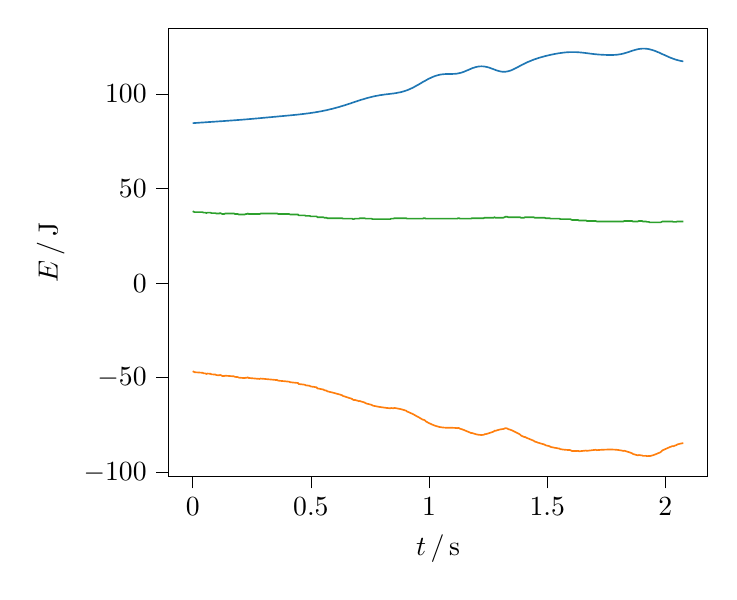
\begin{tikzpicture}

\definecolor{darkgray176}{RGB}{176,176,176}
\definecolor{darkorange25512714}{RGB}{255,127,14}
\definecolor{forestgreen4416044}{RGB}{44,160,44}
\definecolor{steelblue31119180}{RGB}{31,119,180}

\begin{axis}[
tick align=outside,
tick pos=left,
x grid style={darkgray176},
xlabel={\(\displaystyle t\,/\,\mathrm{s}\)},
xmin=-0.1038, xmax=2.1798,
xtick style={color=black},
y grid style={darkgray176},
ylabel={\(\displaystyle E\,/\,\mathrm{J}\)},
ymin=-102.273, ymax=134.733,
ytick style={color=black}
]
\addplot [semithick, steelblue31119180]
table {%
0 84.55
0.004 84.58
0.008 84.62
0.012 84.65
0.017 84.69
0.021 84.72
0.025 84.76
0.029 84.8
0.033 84.83
0.037 84.87
0.042 84.9
0.046 84.94
0.05 84.97
0.054 85.01
0.058 85.04
0.062 85.08
0.067 85.12
0.071 85.15
0.075 85.19
0.079 85.22
0.083 85.26
0.087 85.29
0.092 85.33
0.096 85.36
0.1 85.4
0.104 85.43
0.108 85.47
0.112 85.5
0.116 85.54
0.121 85.57
0.125 85.61
0.129 85.64
0.133 85.68
0.137 85.72
0.141 85.76
0.146 85.79
0.15 85.83
0.154 85.87
0.158 85.91
0.162 85.94
0.166 85.98
0.171 86.02
0.175 86.06
0.179 86.09
0.183 86.13
0.187 86.17
0.191 86.21
0.195 86.25
0.2 86.29
0.204 86.33
0.208 86.37
0.212 86.41
0.216 86.45
0.22 86.49
0.225 86.54
0.229 86.58
0.233 86.62
0.237 86.67
0.241 86.71
0.245 86.76
0.25 86.81
0.254 86.85
0.258 86.9
0.262 86.94
0.266 86.99
0.27 87.04
0.275 87.08
0.279 87.13
0.283 87.18
0.287 87.23
0.291 87.27
0.295 87.32
0.299 87.37
0.304 87.42
0.308 87.47
0.312 87.52
0.316 87.56
0.32 87.61
0.324 87.66
0.329 87.71
0.333 87.75
0.337 87.8
0.341 87.85
0.345 87.9
0.349 87.94
0.354 87.99
0.358 88.04
0.362 88.09
0.366 88.14
0.37 88.19
0.374 88.23
0.379 88.28
0.383 88.33
0.387 88.38
0.391 88.43
0.395 88.48
0.399 88.52
0.403 88.57
0.408 88.62
0.412 88.67
0.416 88.72
0.42 88.77
0.424 88.82
0.428 88.87
0.433 88.93
0.437 88.98
0.441 89.03
0.445 89.08
0.449 89.14
0.453 89.2
0.458 89.25
0.462 89.32
0.466 89.38
0.47 89.44
0.474 89.5
0.478 89.57
0.482 89.63
0.487 89.7
0.491 89.77
0.495 89.84
0.499 89.92
0.503 89.99
0.507 90.07
0.512 90.15
0.516 90.23
0.52 90.31
0.524 90.4
0.528 90.49
0.532 90.58
0.537 90.68
0.541 90.77
0.545 90.87
0.549 90.97
0.553 91.08
0.557 91.19
0.562 91.3
0.566 91.41
0.57 91.53
0.574 91.64
0.578 91.77
0.582 91.89
0.586 92.02
0.591 92.15
0.595 92.28
0.599 92.42
0.603 92.56
0.607 92.7
0.611 92.84
0.616 92.99
0.62 93.14
0.624 93.29
0.628 93.45
0.632 93.6
0.636 93.76
0.641 93.92
0.645 94.09
0.649 94.26
0.653 94.42
0.657 94.59
0.661 94.76
0.666 94.93
0.67 95.1
0.674 95.28
0.678 95.45
0.682 95.62
0.686 95.8
0.69 95.97
0.695 96.14
0.699 96.32
0.703 96.49
0.707 96.65
0.711 96.82
0.715 96.98
0.72 97.14
0.724 97.3
0.728 97.45
0.732 97.6
0.736 97.75
0.74 97.9
0.745 98.04
0.749 98.17
0.753 98.3
0.757 98.43
0.761 98.55
0.765 98.67
0.769 98.78
0.774 98.89
0.778 98.99
0.782 99.09
0.786 99.19
0.79 99.27
0.794 99.36
0.799 99.44
0.803 99.52
0.807 99.59
0.811 99.66
0.815 99.73
0.819 99.79
0.824 99.86
0.828 99.92
0.832 99.98
0.836 100.04
0.84 100.11
0.844 100.17
0.849 100.24
0.853 100.31
0.857 100.39
0.861 100.47
0.865 100.56
0.869 100.66
0.873 100.76
0.878 100.87
0.882 100.99
0.886 101.12
0.89 101.27
0.894 101.42
0.898 101.58
0.903 101.76
0.907 101.95
0.911 102.15
0.915 102.36
0.919 102.59
0.923 102.83
0.928 103.07
0.932 103.33
0.936 103.6
0.94 103.88
0.944 104.16
0.948 104.45
0.953 104.74
0.957 105.04
0.961 105.34
0.965 105.64
0.969 105.94
0.973 106.24
0.977 106.54
0.982 106.84
0.986 107.13
0.99 107.42
0.994 107.7
0.998 107.97
1.002 108.23
1.007 108.48
1.011 108.72
1.015 108.94
1.019 109.15
1.023 109.35
1.027 109.53
1.032 109.7
1.036 109.85
1.04 109.99
1.044 110.11
1.048 110.21
1.052 110.3
1.057 110.37
1.061 110.43
1.065 110.47
1.069 110.5
1.073 110.53
1.077 110.54
1.081 110.55
1.086 110.55
1.09 110.55
1.094 110.56
1.098 110.56
1.102 110.58
1.106 110.6
1.111 110.64
1.115 110.69
1.119 110.76
1.123 110.84
1.127 110.95
1.131 111.07
1.136 111.21
1.14 111.37
1.144 111.55
1.148 111.74
1.152 111.95
1.156 112.17
1.16 112.39
1.165 112.61
1.169 112.84
1.173 113.06
1.177 113.28
1.181 113.49
1.185 113.69
1.19 113.87
1.194 114.04
1.198 114.19
1.202 114.31
1.206 114.42
1.21 114.5
1.215 114.55
1.219 114.58
1.223 114.59
1.227 114.57
1.231 114.53
1.235 114.46
1.24 114.37
1.244 114.26
1.248 114.13
1.252 113.98
1.256 113.82
1.26 113.64
1.264 113.45
1.269 113.26
1.273 113.06
1.277 112.86
1.281 112.67
1.285 112.49
1.289 112.32
1.294 112.16
1.298 112.02
1.302 111.9
1.306 111.81
1.31 111.74
1.314 111.71
1.319 111.7
1.323 111.73
1.327 111.79
1.331 111.88
1.335 112
1.339 112.14
1.344 112.32
1.348 112.51
1.352 112.73
1.356 112.96
1.36 113.2
1.364 113.46
1.368 113.73
1.373 114
1.377 114.27
1.381 114.55
1.385 114.83
1.389 115.1
1.393 115.37
1.398 115.63
1.402 115.89
1.406 116.15
1.41 116.4
1.414 116.64
1.418 116.87
1.423 117.1
1.427 117.32
1.431 117.53
1.435 117.74
1.439 117.94
1.443 118.13
1.447 118.32
1.452 118.5
1.456 118.68
1.46 118.85
1.464 119.01
1.468 119.17
1.472 119.33
1.477 119.48
1.481 119.63
1.485 119.77
1.489 119.91
1.493 120.04
1.497 120.17
1.502 120.3
1.506 120.42
1.51 120.54
1.514 120.66
1.518 120.77
1.522 120.88
1.527 120.98
1.531 121.09
1.535 121.18
1.539 121.28
1.543 121.37
1.547 121.45
1.551 121.54
1.556 121.61
1.56 121.69
1.564 121.76
1.568 121.82
1.572 121.88
1.576 121.93
1.581 121.98
1.585 122.02
1.589 122.05
1.593 122.08
1.597 122.1
1.601 122.11
1.606 122.12
1.61 122.12
1.614 122.12
1.618 122.11
1.622 122.09
1.626 122.06
1.631 122.03
1.635 121.99
1.639 121.95
1.643 121.9
1.647 121.85
1.651 121.79
1.655 121.73
1.66 121.67
1.664 121.6
1.668 121.53
1.672 121.47
1.676 121.4
1.68 121.33
1.685 121.26
1.689 121.2
1.693 121.14
1.697 121.08
1.701 121.02
1.705 120.97
1.71 120.92
1.714 120.87
1.718 120.83
1.722 120.79
1.726 120.76
1.73 120.72
1.734 120.7
1.739 120.67
1.743 120.65
1.747 120.63
1.751 120.61
1.755 120.6
1.759 120.59
1.764 120.58
1.768 120.58
1.772 120.58
1.776 120.59
1.78 120.61
1.784 120.63
1.789 120.67
1.793 120.71
1.797 120.76
1.801 120.83
1.805 120.9
1.809 120.99
1.814 121.09
1.818 121.2
1.822 121.32
1.826 121.46
1.83 121.61
1.834 121.76
1.838 121.92
1.843 122.09
1.847 122.26
1.851 122.44
1.855 122.61
1.859 122.78
1.863 122.95
1.868 123.11
1.872 123.26
1.876 123.4
1.88 123.53
1.884 123.64
1.888 123.74
1.893 123.82
1.897 123.88
1.901 123.93
1.905 123.95
1.909 123.96
1.913 123.94
1.918 123.9
1.922 123.85
1.926 123.77
1.93 123.68
1.934 123.57
1.938 123.44
1.942 123.3
1.947 123.14
1.951 122.97
1.955 122.78
1.959 122.59
1.963 122.38
1.967 122.16
1.972 121.94
1.976 121.71
1.98 121.48
1.984 121.24
1.988 121
1.992 120.77
1.997 120.53
2.001 120.3
2.005 120.07
2.009 119.84
2.013 119.61
2.017 119.39
2.021 119.17
2.026 118.96
2.03 118.76
2.034 118.57
2.038 118.39
2.042 118.21
2.046 118.05
2.051 117.89
2.055 117.75
2.059 117.62
2.063 117.5
2.067 117.39
2.071 117.29
2.076 117.2
};
\addplot [semithick, darkorange25512714]
table {%
0 -46.57
0.004 -46.85
0.008 -47.12
0.012 -47.16
0.017 -47.2
0.021 -47.23
0.025 -47.27
0.029 -47.3
0.033 -47.34
0.037 -47.37
0.042 -47.41
0.046 -47.69
0.05 -47.72
0.054 -47.76
0.058 -48.04
0.062 -47.83
0.067 -47.87
0.071 -47.9
0.075 -47.94
0.079 -48.22
0.083 -48.26
0.087 -48.29
0.092 -48.33
0.096 -48.36
0.1 -48.64
0.104 -48.67
0.108 -48.71
0.112 -48.74
0.116 -48.53
0.121 -48.81
0.125 -49.09
0.129 -49.13
0.133 -49.17
0.137 -48.96
0.141 -49
0.146 -49.04
0.15 -49.07
0.154 -49.11
0.158 -49.15
0.162 -49.19
0.166 -49.22
0.171 -49.26
0.175 -49.3
0.179 -49.58
0.183 -49.62
0.187 -49.66
0.191 -49.7
0.195 -49.98
0.2 -50.02
0.204 -50.06
0.208 -50.11
0.212 -50.15
0.216 -50.19
0.22 -50.23
0.225 -50.02
0.229 -50.07
0.233 -49.86
0.237 -50.15
0.241 -50.2
0.245 -50.25
0.25 -50.29
0.254 -50.34
0.258 -50.39
0.262 -50.43
0.266 -50.48
0.27 -50.53
0.275 -50.57
0.279 -50.62
0.283 -50.67
0.287 -50.47
0.291 -50.52
0.295 -50.56
0.299 -50.61
0.304 -50.66
0.308 -50.71
0.312 -50.76
0.316 -50.81
0.32 -50.85
0.324 -50.9
0.329 -50.95
0.333 -51
0.337 -51.04
0.341 -51.09
0.345 -51.14
0.349 -51.19
0.354 -51.23
0.358 -51.28
0.362 -51.57
0.366 -51.62
0.37 -51.67
0.374 -51.72
0.379 -51.77
0.383 -51.82
0.387 -51.87
0.391 -51.92
0.395 -51.96
0.399 -52.01
0.403 -52.06
0.408 -52.11
0.412 -52.4
0.416 -52.45
0.42 -52.5
0.424 -52.56
0.428 -52.61
0.433 -52.66
0.437 -52.71
0.441 -52.76
0.445 -52.81
0.449 -53.36
0.453 -53.42
0.458 -53.48
0.462 -53.54
0.466 -53.6
0.47 -53.66
0.474 -53.72
0.478 -54.03
0.482 -54.1
0.487 -54.17
0.491 -54.24
0.495 -54.31
0.499 -54.63
0.503 -54.71
0.507 -54.78
0.512 -54.86
0.516 -54.94
0.52 -55.03
0.524 -55.11
0.528 -55.69
0.532 -55.78
0.537 -55.88
0.541 -55.98
0.545 -56.08
0.549 -56.18
0.553 -56.28
0.557 -56.63
0.562 -56.74
0.566 -56.86
0.57 -57.22
0.574 -57.34
0.578 -57.46
0.582 -57.59
0.586 -57.71
0.591 -57.84
0.595 -57.98
0.599 -58.11
0.603 -58.25
0.607 -58.39
0.611 -58.54
0.616 -58.68
0.62 -58.83
0.624 -58.98
0.628 -59.14
0.632 -59.3
0.636 -59.7
0.641 -59.86
0.645 -60.03
0.649 -60.19
0.653 -60.36
0.657 -60.53
0.661 -60.7
0.666 -60.87
0.67 -61.04
0.674 -61.22
0.678 -61.63
0.682 -61.81
0.686 -61.74
0.69 -61.91
0.695 -62.08
0.699 -62.25
0.703 -62.42
0.707 -62.35
0.711 -62.51
0.715 -62.68
0.72 -62.84
0.724 -62.99
0.728 -63.15
0.732 -63.54
0.736 -63.69
0.74 -63.83
0.745 -63.97
0.749 -64.11
0.753 -64.24
0.757 -64.37
0.761 -64.73
0.765 -64.85
0.769 -64.97
0.774 -65.07
0.778 -65.18
0.782 -65.28
0.786 -65.37
0.79 -65.46
0.794 -65.54
0.799 -65.62
0.803 -65.7
0.807 -65.77
0.811 -65.84
0.815 -65.91
0.819 -65.98
0.824 -66.04
0.828 -66.1
0.832 -66.16
0.836 -66.23
0.84 -66.05
0.844 -66.11
0.849 -66.18
0.853 -66.01
0.857 -66.08
0.861 -66.17
0.865 -66.26
0.869 -66.35
0.873 -66.45
0.878 -66.57
0.882 -66.69
0.886 -66.82
0.89 -66.96
0.894 -67.11
0.898 -67.28
0.903 -67.45
0.907 -67.89
0.911 -68.09
0.915 -68.3
0.919 -68.53
0.923 -68.77
0.928 -69.01
0.932 -69.27
0.936 -69.54
0.94 -69.81
0.944 -70.1
0.948 -70.39
0.953 -70.68
0.957 -70.98
0.961 -71.28
0.965 -71.58
0.969 -71.88
0.973 -72.18
0.977 -72.24
0.982 -72.53
0.986 -73.07
0.99 -73.36
0.994 -73.63
0.998 -73.9
1.002 -74.17
1.007 -74.42
1.011 -74.65
1.015 -74.88
1.019 -75.09
1.023 -75.29
1.027 -75.47
1.032 -75.64
1.036 -75.79
1.04 -75.93
1.044 -76.05
1.048 -76.15
1.052 -76.24
1.057 -76.31
1.061 -76.37
1.065 -76.41
1.069 -76.44
1.073 -76.46
1.077 -76.48
1.081 -76.49
1.086 -76.49
1.09 -76.49
1.094 -76.49
1.098 -76.5
1.102 -76.52
1.106 -76.54
1.111 -76.58
1.115 -76.63
1.119 -76.7
1.123 -76.54
1.127 -76.64
1.131 -77.01
1.136 -77.15
1.14 -77.31
1.144 -77.49
1.148 -77.68
1.152 -77.89
1.156 -78.1
1.16 -78.33
1.165 -78.55
1.169 -78.78
1.173 -79
1.177 -79.22
1.181 -79.19
1.185 -79.38
1.19 -79.57
1.194 -79.73
1.198 -79.88
1.202 -80.01
1.206 -80.11
1.21 -80.19
1.215 -80.25
1.219 -80.28
1.223 -80.28
1.227 -80.26
1.231 -80.22
1.235 -79.91
1.24 -79.82
1.244 -79.71
1.248 -79.58
1.252 -79.43
1.256 -79.26
1.26 -79.09
1.264 -78.9
1.269 -78.71
1.273 -78.51
1.277 -78.07
1.281 -78.12
1.285 -77.94
1.289 -77.77
1.294 -77.61
1.298 -77.47
1.302 -77.35
1.306 -77.26
1.31 -77.19
1.314 -77.15
1.319 -76.9
1.323 -76.69
1.327 -76.75
1.331 -76.84
1.335 -77.2
1.339 -77.35
1.344 -77.52
1.348 -77.71
1.352 -77.93
1.356 -78.16
1.36 -78.41
1.364 -78.66
1.368 -78.93
1.373 -79.2
1.377 -79.48
1.381 -79.75
1.385 -80.03
1.389 -80.55
1.393 -80.82
1.398 -81.08
1.402 -81.34
1.406 -81.35
1.41 -81.6
1.414 -81.84
1.418 -82.07
1.423 -82.3
1.427 -82.52
1.431 -82.73
1.435 -82.94
1.439 -83.14
1.443 -83.33
1.447 -83.76
1.452 -83.95
1.456 -84.12
1.46 -84.3
1.464 -84.46
1.468 -84.62
1.472 -84.78
1.477 -84.93
1.481 -85.08
1.485 -85.22
1.489 -85.36
1.493 -85.73
1.497 -85.86
1.502 -85.99
1.506 -86.11
1.51 -86.23
1.514 -86.59
1.518 -86.71
1.522 -86.82
1.527 -86.92
1.531 -87.03
1.535 -87.12
1.539 -87.22
1.543 -87.31
1.547 -87.39
1.551 -87.47
1.556 -87.8
1.56 -87.87
1.564 -87.94
1.568 -88.01
1.572 -88.06
1.576 -88.12
1.581 -88.16
1.585 -88.2
1.589 -88.24
1.593 -88.26
1.597 -88.28
1.601 -88.54
1.606 -88.8
1.61 -88.8
1.614 -88.79
1.618 -88.78
1.622 -88.76
1.626 -88.74
1.631 -88.71
1.635 -88.91
1.639 -88.87
1.643 -88.82
1.647 -88.77
1.651 -88.71
1.655 -88.65
1.66 -88.59
1.664 -88.52
1.668 -88.7
1.672 -88.63
1.676 -88.56
1.68 -88.5
1.685 -88.43
1.689 -88.36
1.693 -88.3
1.697 -88.24
1.701 -88.18
1.705 -88.13
1.71 -88.33
1.714 -88.28
1.718 -88.24
1.722 -88.2
1.726 -88.17
1.73 -88.13
1.734 -88.11
1.739 -88.08
1.743 -88.06
1.747 -88.04
1.751 -88.02
1.755 -88.01
1.759 -88
1.764 -87.99
1.768 -87.99
1.772 -87.99
1.776 -88
1.78 -88.02
1.784 -88.04
1.789 -88.08
1.793 -88.12
1.797 -88.17
1.801 -88.24
1.805 -88.31
1.809 -88.4
1.814 -88.5
1.818 -88.61
1.822 -88.73
1.826 -88.62
1.83 -88.77
1.834 -88.93
1.838 -89.09
1.843 -89.26
1.847 -89.43
1.851 -89.6
1.855 -89.78
1.859 -89.95
1.863 -90.36
1.868 -90.52
1.872 -90.67
1.876 -90.81
1.88 -90.94
1.884 -91.05
1.888 -90.9
1.893 -90.98
1.897 -91.05
1.901 -91.09
1.905 -91.36
1.909 -91.36
1.913 -91.35
1.918 -91.31
1.922 -91.5
1.926 -91.43
1.93 -91.34
1.934 -91.47
1.938 -91.34
1.942 -91.2
1.947 -91.04
1.951 -90.87
1.955 -90.68
1.959 -90.49
1.963 -90.28
1.967 -90.06
1.972 -89.84
1.976 -89.61
1.98 -89.38
1.984 -88.89
1.988 -88.41
1.992 -88.18
1.997 -87.94
2.001 -87.71
2.005 -87.47
2.009 -87.24
2.013 -87.02
2.017 -86.8
2.021 -86.58
2.026 -86.37
2.03 -86.17
2.034 -86.22
2.038 -86.04
2.042 -85.87
2.046 -85.7
2.051 -85.3
2.055 -85.16
2.059 -85.03
2.063 -84.91
2.067 -84.8
2.071 -84.7
2.076 -84.61
};
\addplot [semithick, forestgreen4416044]
table {%
0 37.98
0.004 37.74
0.008 37.49
0.012 37.49
0.017 37.49
0.021 37.49
0.025 37.49
0.029 37.49
0.033 37.49
0.037 37.49
0.042 37.49
0.046 37.25
0.05 37.25
0.054 37.25
0.058 37
0.062 37.25
0.067 37.25
0.071 37.25
0.075 37.25
0.079 37
0.083 37
0.087 37
0.092 37
0.096 37
0.1 36.76
0.104 36.76
0.108 36.76
0.112 36.76
0.116 37
0.121 36.76
0.125 36.51
0.129 36.51
0.133 36.51
0.137 36.76
0.141 36.76
0.146 36.76
0.15 36.76
0.154 36.76
0.158 36.76
0.162 36.76
0.166 36.76
0.171 36.76
0.175 36.76
0.179 36.51
0.183 36.51
0.187 36.51
0.191 36.51
0.195 36.27
0.2 36.27
0.204 36.27
0.208 36.27
0.212 36.27
0.216 36.27
0.22 36.27
0.225 36.51
0.229 36.51
0.233 36.76
0.237 36.51
0.241 36.51
0.245 36.51
0.25 36.51
0.254 36.51
0.258 36.51
0.262 36.51
0.266 36.51
0.27 36.51
0.275 36.51
0.279 36.51
0.283 36.51
0.287 36.76
0.291 36.76
0.295 36.76
0.299 36.76
0.304 36.76
0.308 36.76
0.312 36.76
0.316 36.76
0.32 36.76
0.324 36.76
0.329 36.76
0.333 36.76
0.337 36.76
0.341 36.76
0.345 36.76
0.349 36.76
0.354 36.76
0.358 36.76
0.362 36.51
0.366 36.51
0.37 36.51
0.374 36.51
0.379 36.51
0.383 36.51
0.387 36.51
0.391 36.51
0.395 36.51
0.399 36.51
0.403 36.51
0.408 36.51
0.412 36.27
0.416 36.27
0.42 36.27
0.424 36.27
0.428 36.27
0.433 36.27
0.437 36.27
0.441 36.27
0.445 36.27
0.449 35.78
0.453 35.78
0.458 35.78
0.462 35.78
0.466 35.78
0.47 35.78
0.474 35.78
0.478 35.53
0.482 35.53
0.487 35.53
0.491 35.53
0.495 35.53
0.499 35.29
0.503 35.29
0.507 35.29
0.512 35.29
0.516 35.29
0.52 35.29
0.524 35.29
0.528 34.8
0.532 34.8
0.537 34.8
0.541 34.8
0.545 34.8
0.549 34.8
0.553 34.8
0.557 34.55
0.562 34.55
0.566 34.55
0.57 34.31
0.574 34.31
0.578 34.31
0.582 34.31
0.586 34.31
0.591 34.31
0.595 34.31
0.599 34.31
0.603 34.31
0.607 34.31
0.611 34.31
0.616 34.31
0.62 34.31
0.624 34.31
0.628 34.31
0.632 34.31
0.636 34.06
0.641 34.06
0.645 34.06
0.649 34.06
0.653 34.06
0.657 34.06
0.661 34.06
0.666 34.06
0.67 34.06
0.674 34.06
0.678 33.82
0.682 33.82
0.686 34.06
0.69 34.06
0.695 34.06
0.699 34.06
0.703 34.06
0.707 34.31
0.711 34.31
0.715 34.31
0.72 34.31
0.724 34.31
0.728 34.31
0.732 34.06
0.736 34.06
0.74 34.06
0.745 34.06
0.749 34.06
0.753 34.06
0.757 34.06
0.761 33.82
0.765 33.82
0.769 33.82
0.774 33.82
0.778 33.82
0.782 33.82
0.786 33.82
0.79 33.82
0.794 33.82
0.799 33.82
0.803 33.82
0.807 33.82
0.811 33.82
0.815 33.82
0.819 33.82
0.824 33.82
0.828 33.82
0.832 33.82
0.836 33.82
0.84 34.06
0.844 34.06
0.849 34.06
0.853 34.31
0.857 34.31
0.861 34.31
0.865 34.31
0.869 34.31
0.873 34.31
0.878 34.31
0.882 34.31
0.886 34.31
0.89 34.31
0.894 34.31
0.898 34.31
0.903 34.31
0.907 34.06
0.911 34.06
0.915 34.06
0.919 34.06
0.923 34.06
0.928 34.06
0.932 34.06
0.936 34.06
0.94 34.06
0.944 34.06
0.948 34.06
0.953 34.06
0.957 34.06
0.961 34.06
0.965 34.06
0.969 34.06
0.973 34.06
0.977 34.31
0.982 34.31
0.986 34.06
0.99 34.06
0.994 34.06
0.998 34.06
1.002 34.06
1.007 34.06
1.011 34.06
1.015 34.06
1.019 34.06
1.023 34.06
1.027 34.06
1.032 34.06
1.036 34.06
1.04 34.06
1.044 34.06
1.048 34.06
1.052 34.06
1.057 34.06
1.061 34.06
1.065 34.06
1.069 34.06
1.073 34.06
1.077 34.06
1.081 34.06
1.086 34.06
1.09 34.06
1.094 34.06
1.098 34.06
1.102 34.06
1.106 34.06
1.111 34.06
1.115 34.06
1.119 34.06
1.123 34.31
1.127 34.31
1.131 34.06
1.136 34.06
1.14 34.06
1.144 34.06
1.148 34.06
1.152 34.06
1.156 34.06
1.16 34.06
1.165 34.06
1.169 34.06
1.173 34.06
1.177 34.06
1.181 34.31
1.185 34.31
1.19 34.31
1.194 34.31
1.198 34.31
1.202 34.31
1.206 34.31
1.21 34.31
1.215 34.31
1.219 34.31
1.223 34.31
1.227 34.31
1.231 34.31
1.235 34.55
1.24 34.55
1.244 34.55
1.248 34.55
1.252 34.55
1.256 34.55
1.26 34.55
1.264 34.55
1.269 34.55
1.273 34.55
1.277 34.8
1.281 34.55
1.285 34.55
1.289 34.55
1.294 34.55
1.298 34.55
1.302 34.55
1.306 34.55
1.31 34.55
1.314 34.55
1.319 34.8
1.323 35.04
1.327 35.04
1.331 35.04
1.335 34.8
1.339 34.8
1.344 34.8
1.348 34.8
1.352 34.8
1.356 34.8
1.36 34.8
1.364 34.8
1.368 34.8
1.373 34.8
1.377 34.8
1.381 34.8
1.385 34.8
1.389 34.55
1.393 34.55
1.398 34.55
1.402 34.55
1.406 34.8
1.41 34.8
1.414 34.8
1.418 34.8
1.423 34.8
1.427 34.8
1.431 34.8
1.435 34.8
1.439 34.8
1.443 34.8
1.447 34.55
1.452 34.55
1.456 34.55
1.46 34.55
1.464 34.55
1.468 34.55
1.472 34.55
1.477 34.55
1.481 34.55
1.485 34.55
1.489 34.55
1.493 34.31
1.497 34.31
1.502 34.31
1.506 34.31
1.51 34.31
1.514 34.06
1.518 34.06
1.522 34.06
1.527 34.06
1.531 34.06
1.535 34.06
1.539 34.06
1.543 34.06
1.547 34.06
1.551 34.06
1.556 33.82
1.56 33.82
1.564 33.82
1.568 33.82
1.572 33.82
1.576 33.82
1.581 33.82
1.585 33.82
1.589 33.82
1.593 33.82
1.597 33.82
1.601 33.57
1.606 33.33
1.61 33.33
1.614 33.33
1.618 33.33
1.622 33.33
1.626 33.33
1.631 33.33
1.635 33.08
1.639 33.08
1.643 33.08
1.647 33.08
1.651 33.08
1.655 33.08
1.66 33.08
1.664 33.08
1.668 32.84
1.672 32.84
1.676 32.84
1.68 32.84
1.685 32.84
1.689 32.84
1.693 32.84
1.697 32.84
1.701 32.84
1.705 32.84
1.71 32.59
1.714 32.59
1.718 32.59
1.722 32.59
1.726 32.59
1.73 32.59
1.734 32.59
1.739 32.59
1.743 32.59
1.747 32.59
1.751 32.59
1.755 32.59
1.759 32.59
1.764 32.59
1.768 32.59
1.772 32.59
1.776 32.59
1.78 32.59
1.784 32.59
1.789 32.59
1.793 32.59
1.797 32.59
1.801 32.59
1.805 32.59
1.809 32.59
1.814 32.59
1.818 32.59
1.822 32.59
1.826 32.84
1.83 32.84
1.834 32.84
1.838 32.84
1.843 32.84
1.847 32.84
1.851 32.84
1.855 32.84
1.859 32.84
1.863 32.59
1.868 32.59
1.872 32.59
1.876 32.59
1.88 32.59
1.884 32.59
1.888 32.84
1.893 32.84
1.897 32.84
1.901 32.84
1.905 32.59
1.909 32.59
1.913 32.59
1.918 32.59
1.922 32.35
1.926 32.35
1.93 32.35
1.934 32.1
1.938 32.1
1.942 32.1
1.947 32.1
1.951 32.1
1.955 32.1
1.959 32.1
1.963 32.1
1.967 32.1
1.972 32.1
1.976 32.1
1.98 32.1
1.984 32.35
1.988 32.59
1.992 32.59
1.997 32.59
2.001 32.59
2.005 32.59
2.009 32.59
2.013 32.59
2.017 32.59
2.021 32.59
2.026 32.59
2.03 32.59
2.034 32.35
2.038 32.35
2.042 32.35
2.046 32.35
2.051 32.59
2.055 32.59
2.059 32.59
2.063 32.59
2.067 32.59
2.071 32.59
2.076 32.59
};
\end{axis}

\end{tikzpicture}

            \end{adjustbox}
            \caption{\(\delta t^*=0.001\)}
        \end{subfigure}
        \hfill
        \begin{subfigure}[h]{0.32\linewidth}
            \begin{adjustbox}{width=\linewidth}
            % This file was created with tikzplotlib v0.10.1.
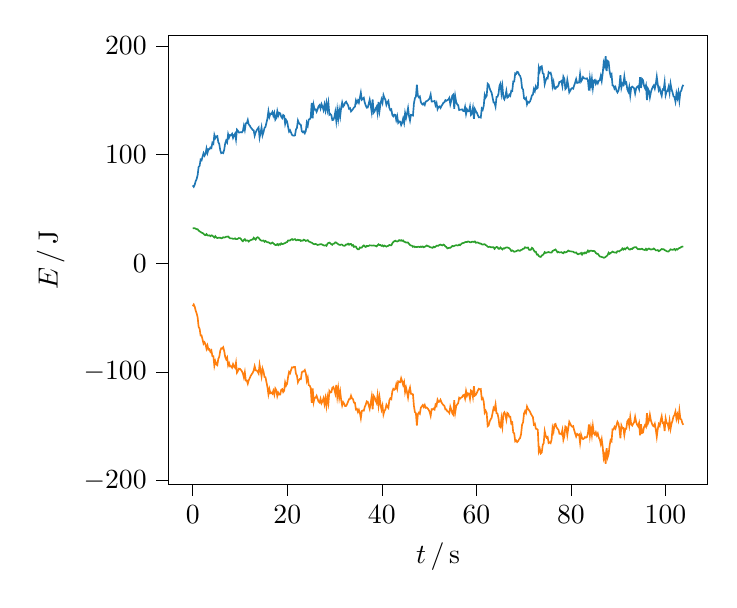
\begin{tikzpicture}

\definecolor{darkgray176}{RGB}{176,176,176}
\definecolor{darkorange25512714}{RGB}{255,127,14}
\definecolor{forestgreen4416044}{RGB}{44,160,44}
\definecolor{steelblue31119180}{RGB}{31,119,180}

\begin{axis}[
tick align=outside,
tick pos=left,
x grid style={darkgray176},
xlabel={\(\displaystyle t\,/\,\mathrm{s}\)},
xmin=-5.1889, xmax=108.9669,
xtick style={color=black},
y grid style={darkgray176},
ylabel={\(\displaystyle E\,/\,\mathrm{J}\)},
ymin=-203.363, ymax=209.203,
ytick style={color=black}
]
\addplot [semithick, steelblue31119180]
table {%
0 71.57
0.208 70.26
0.416 72.12
0.624 75.41
0.832 77.4
1.04 81.09
1.248 88.56
1.456 89.52
1.664 95.3
1.872 94.62
2.08 98.05
2.288 101.2
2.496 98.86
2.704 100.52
2.912 105.48
3.12 101.42
3.328 104.95
3.536 104.75
3.744 106.48
3.951 105.91
4.159 110.85
4.367 109.88
4.575 117.97
4.783 115.07
4.991 116.63
5.199 116.98
5.407 111.44
5.615 109.54
5.823 103.98
6.031 101.23
6.239 101.74
6.447 101.24
6.655 104.27
6.863 110.04
7.071 112.76
7.279 111.06
7.487 118.67
7.695 115.62
7.903 117.86
8.111 117.7
8.319 119.01
8.527 115.34
8.735 117.72
8.943 119.14
9.151 113.74
9.359 122.88
9.567 121.81
9.775 120.16
9.983 120.3
10.191 120.54
10.399 120.34
10.607 121.63
10.815 126.4
11.023 122.5
11.231 128.68
11.438 128.84
11.646 131.77
11.854 127.54
12.062 126.66
12.27 124.8
12.478 123.87
12.686 122.54
12.894 122.23
13.102 117.24
13.31 120.27
13.518 122.05
13.726 123.66
13.934 124.87
14.142 115.53
14.35 119.94
14.558 124.83
14.766 117.62
14.974 120.59
15.182 124.39
15.39 125.43
15.598 129.18
15.806 133.26
16.014 139.83
16.222 134.62
16.43 137.59
16.638 137.31
16.846 139.06
17.054 135.62
17.262 138.37
17.47 132.05
17.678 133.6
17.886 139.85
18.094 135.73
18.302 138.33
18.51 137.8
18.718 134.77
18.926 133.43
19.133 136.36
19.341 135.62
19.549 128.17
19.757 131.78
19.965 130.35
20.173 125.52
20.381 121.03
20.589 122.24
20.797 120.12
21.005 118.01
21.213 117.48
21.421 117.28
21.629 117.58
21.837 122.95
22.045 124.5
22.253 131.25
22.461 128.92
22.669 127.93
22.877 127.19
23.085 121.24
23.293 120.39
23.501 121.27
23.709 119.52
23.917 121.49
24.125 129.16
24.333 126.48
24.541 132.18
24.749 132.41
24.957 133.97
25.165 147.35
25.373 133.34
25.581 145.42
25.789 141.26
25.997 141.51
26.205 139.24
26.413 141.5
26.62 144.41
26.828 145.43
27.036 142.31
27.244 146.34
27.452 144.12
27.66 140.91
27.868 145.87
28.076 140.78
28.284 147.36
28.492 141.2
28.7 147.39
28.908 136.54
29.116 137.21
29.324 136.19
29.532 131.65
29.74 131.86
29.948 134.13
30.156 139.04
30.364 130.95
30.572 140.76
30.78 132.78
30.988 140.85
31.196 135.08
31.404 143.15
31.612 147.83
31.82 144.08
32.028 145.35
32.236 147.69
32.444 148.55
32.652 146.83
32.86 145.32
33.068 142.1
33.276 142.6
33.484 139.64
33.692 140.65
33.9 141.79
34.108 143.28
34.315 143.95
34.523 149.82
34.731 147.63
34.939 149.7
35.147 147.63
35.355 152.19
35.563 156.83
35.771 150.36
35.979 151.16
36.187 152.11
36.395 147.63
36.603 145.12
36.811 143.04
37.019 143.17
37.227 146.58
37.435 150.4
37.643 145.13
37.851 139.3
38.059 150.64
38.267 138.42
38.475 139.6
38.683 142.21
38.891 143.9
39.099 138.02
39.307 148.32
39.515 140.03
39.723 146.69
39.931 150.69
40.139 147.56
40.347 154.64
40.555 152.08
40.763 150.34
40.971 145.61
41.179 147.91
41.387 149.29
41.595 142.83
41.802 140.83
42.01 141.57
42.218 136.37
42.426 135.12
42.634 136.7
42.842 136.39
43.05 131.76
43.258 135.28
43.466 129.17
43.674 130.46
43.882 130.25
44.09 127.06
44.298 129.09
44.506 132.95
44.714 129.06
44.922 138.06
45.13 133.65
45.338 137.77
45.546 142.65
45.754 135.31
45.962 131.22
46.17 136.5
46.378 136.38
46.586 135.83
46.794 146.96
47.002 151.86
47.21 153.12
47.418 164.23
47.626 154.02
47.834 152.62
48.042 153.44
48.25 148.38
48.458 146.71
48.666 145.91
48.874 147.05
49.082 145.59
49.29 148.69
49.497 149.15
49.705 149.57
49.913 150.49
50.121 151.85
50.329 155.12
50.537 148.8
50.745 148.8
50.953 148.89
51.161 149.26
51.369 145.22
51.577 147.38
51.785 141.76
51.993 143.79
52.201 144.28
52.409 142.81
52.617 144.61
52.825 145.94
53.033 147.68
53.241 147.96
53.449 150.01
53.657 149.43
53.865 150.02
54.073 150.52
54.281 152.08
54.489 146.17
54.697 149.64
54.905 154.07
55.113 155.06
55.321 141.93
55.529 153.55
55.737 148.12
55.945 146.18
56.153 145.21
56.361 140.93
56.569 141.22
56.777 141.3
56.984 141.47
57.192 140.09
57.4 139.91
57.608 143.77
57.816 137.2
58.024 141.45
58.232 139.75
58.44 139.82
58.648 144.05
58.856 136.49
59.064 137.9
59.272 142.85
59.48 132.75
59.688 141.81
59.896 139.86
60.104 138.42
60.312 136.22
60.52 134.14
60.728 134.21
60.936 133.94
61.144 142.31
61.352 141.2
61.56 144.8
61.768 154.88
61.976 152.48
62.184 154.01
62.392 165.13
62.6 164.2
62.808 160.91
63.016 158.53
63.224 156.95
63.432 152.39
63.64 147.83
63.848 147.82
64.056 144.12
64.264 152.88
64.472 153.19
64.679 155.72
64.887 163.24
65.095 165.3
65.303 156.29
65.511 162.69
65.719 152.42
65.927 150.68
66.135 153.46
66.343 158.4
66.551 152.32
66.759 152.94
66.967 155.05
67.175 154.03
67.383 158.66
67.591 158.33
67.799 167.09
68.007 167.05
68.215 174.6
68.423 174.1
68.631 176.1
68.839 175.67
69.047 173.34
69.255 172.34
69.463 169.32
69.671 161.01
69.879 159.73
70.087 151.68
70.295 150.78
70.503 152.01
70.711 146.08
70.919 148.44
71.127 147.7
71.335 148.72
71.543 151.09
71.751 154.44
71.959 155.05
72.166 160.24
72.374 158.25
72.582 162.75
72.79 160.65
72.998 161.42
73.206 179.94
73.414 176.89
73.622 180.8
73.83 181.25
74.038 174.91
74.246 174
74.454 164.74
74.662 168.13
74.87 170.38
75.078 169.93
75.286 175.7
75.494 174.79
75.702 175.28
75.91 172.06
76.118 162.77
76.326 166.65
76.534 160.57
76.742 160.51
76.95 162.32
77.158 162.19
77.366 163.68
77.574 166.85
77.782 166.84
77.99 167.65
78.198 162.98
78.406 171.68
78.614 169.67
78.822 160.2
79.03 161.27
79.238 168.61
79.446 163.42
79.653 157.12
79.861 158.72
80.069 160.47
80.277 161.12
80.485 160.57
80.693 163.64
80.901 166.31
81.109 169.39
81.317 165.81
81.525 166.12
81.733 166.26
81.941 173.99
82.149 167.24
82.357 168.85
82.565 171.29
82.773 170.16
82.981 169.88
83.189 169.68
83.397 170.09
83.605 168.15
83.813 158.77
84.021 170.05
84.229 163.19
84.437 169.68
84.645 161.04
84.853 167.97
85.061 168.66
85.269 165.07
85.477 167.23
85.685 165.38
85.893 167.89
86.101 168.35
86.309 172.19
86.517 167.71
86.725 174.67
86.933 184.42
87.141 181.47
87.348 190.45
87.556 176.68
87.764 186.14
87.972 185.45
88.18 176.71
88.388 172.19
88.596 173.73
88.804 163.56
89.012 163.15
89.22 160.55
89.428 162.06
89.636 158.78
89.844 157.06
90.052 158.64
90.26 163.15
90.468 172.95
90.676 161.51
90.884 165.35
91.092 164.15
91.3 171.62
91.508 165.2
91.716 166.22
91.924 160.05
92.132 157.8
92.34 162.1
92.548 154.17
92.756 161.54
92.964 162.46
93.172 161.69
93.38 160.87
93.588 156.16
93.796 160.8
94.004 162.22
94.212 162.91
94.42 160.21
94.628 171.08
94.835 161.25
95.043 169.54
95.251 168.36
95.459 163.34
95.667 161.1
95.875 163.71
96.083 150.03
96.291 160.55
96.499 158.69
96.707 152.54
96.915 157.18
97.123 160.16
97.331 162.25
97.539 163.62
97.747 160.66
97.955 164.83
98.163 171.52
98.371 164.62
98.579 159.13
98.787 161.15
98.995 156.88
99.203 153.98
99.411 159.94
99.619 159.53
99.827 166.49
100.035 154.64
100.243 157.98
100.451 158.44
100.659 162.11
100.867 156.71
101.075 165.21
101.283 160.17
101.491 157.17
101.699 153.57
101.907 152.85
102.115 148.61
102.323 156.2
102.53 151.98
102.738 157.25
102.946 149.49
103.154 157.42
103.362 158.91
103.57 162.35
103.778 164.13
};
\addplot [semithick, darkorange25512714]
table {%
0 -39.62
0.208 -38.07
0.416 -39.93
0.624 -43.72
0.832 -46.19
1.04 -49.88
1.248 -58.59
1.456 -60.26
1.664 -66.55
1.872 -66.61
2.08 -70.28
2.288 -74.19
2.496 -72.81
2.704 -74.72
2.912 -78.71
3.12 -75.83
3.328 -79.63
3.536 -79.19
3.744 -81.66
3.951 -80.36
4.159 -85.52
4.367 -85.53
4.575 -94.38
4.783 -90.25
4.991 -93.04
5.199 -93.88
5.407 -88.08
5.615 -86.17
5.823 -80.61
6.031 -78.34
6.239 -78.63
6.447 -77.4
6.655 -80.69
6.863 -86.21
7.071 -88.44
7.279 -86.72
7.487 -94.11
7.695 -92.03
7.903 -95.04
8.111 -94.87
8.319 -96.19
8.527 -92.99
8.735 -95.37
8.943 -96.31
9.151 -91.62
9.359 -100.79
9.567 -99.21
9.775 -97.08
9.983 -97.24
10.191 -98.22
10.399 -99.49
10.607 -101.5
10.815 -105.06
11.023 -100.39
11.231 -108.07
11.438 -108
11.646 -110.91
11.854 -107.67
12.062 -105.8
12.27 -103.68
12.478 -102.25
12.686 -100.91
12.894 -98.87
13.102 -94.86
13.31 -98.63
13.518 -98.7
13.726 -99.8
13.934 -101.53
14.142 -93.4
14.35 -98.82
14.558 -104.19
14.766 -96.94
14.974 -99.69
15.182 -104.73
15.39 -105.02
15.598 -109.52
15.806 -114.08
16.014 -120.65
16.222 -115.92
16.43 -119.66
16.638 -119.11
16.846 -120.12
17.054 -117.39
17.262 -120.9
17.47 -115.31
17.678 -116.86
17.886 -122.35
18.094 -119.2
18.302 -120.86
18.51 -120.83
18.718 -116.55
18.926 -115.95
19.133 -118.64
19.341 -117.41
19.549 -109.7
19.757 -112.64
19.965 -110.99
20.173 -104.62
20.381 -100.11
20.589 -101.34
20.797 -98.49
21.005 -95.87
21.213 -96.09
21.421 -95.42
21.629 -95.48
21.837 -101.82
22.045 -103.37
22.253 -109.65
22.461 -107.81
22.669 -106.57
22.877 -106.8
23.085 -100.36
23.293 -99.73
23.501 -99.64
23.709 -98.36
23.917 -101.09
24.125 -108.28
24.333 -105.32
24.541 -112.27
24.749 -112.75
24.957 -114.8
25.165 -128.47
25.373 -115.18
25.581 -127.77
25.789 -123.82
25.997 -123.82
26.205 -122.03
26.413 -124.79
26.62 -127.46
26.828 -128.27
27.036 -124.85
27.244 -128.9
27.452 -127.17
27.66 -124.45
27.868 -129.65
28.076 -124.31
28.284 -131.4
28.492 -123.51
28.7 -128.77
28.908 -117.63
29.116 -119.05
29.324 -118.79
29.532 -114.72
29.74 -113.93
29.948 -116.2
30.156 -119.9
30.364 -112.02
30.572 -122.62
30.78 -115.35
30.988 -123.92
31.196 -118.34
31.404 -125.98
31.612 -130.9
31.82 -127.88
32.028 -129.38
32.236 -131.53
32.444 -131.4
32.652 -129.67
32.86 -127.42
33.068 -125.19
33.276 -124.96
33.484 -121.98
33.692 -124.47
33.9 -125.13
34.108 -128.32
34.315 -128.52
34.523 -134.64
34.731 -134.16
34.939 -136.98
35.147 -134.91
35.355 -137.74
35.563 -142.68
35.771 -135.98
35.979 -135.52
36.187 -135.77
36.395 -132.27
36.603 -130.22
36.811 -127.17
37.019 -127.56
37.227 -130.67
37.435 -134
37.643 -128.77
37.851 -123.17
38.059 -134.52
38.267 -122.06
38.475 -123.51
38.683 -126.32
38.891 -128.49
39.099 -121.59
39.307 -130.94
39.515 -123.36
39.723 -130.01
39.931 -134.78
40.139 -131.15
40.347 -139.19
40.555 -135.89
40.763 -134.64
40.971 -130.4
41.179 -132.24
41.387 -133.34
41.595 -126.1
41.802 -124.38
42.01 -125.12
42.218 -118.16
42.426 -115.7
42.634 -116.53
42.842 -115.72
43.05 -111.58
43.258 -115.35
43.466 -108.77
43.674 -109.29
43.882 -109.56
44.09 -105.87
44.298 -108.65
44.506 -112.03
44.714 -109.34
44.922 -118.62
45.13 -114.67
45.338 -118.81
45.546 -123.71
45.754 -117.58
45.962 -114.48
46.17 -120.26
46.378 -120.38
46.586 -120.79
46.794 -131.47
47.002 -137.1
47.21 -138.04
47.418 -149.46
47.626 -138.98
47.834 -137.57
48.042 -138.64
48.25 -133.05
48.458 -131.85
48.666 -130.58
48.874 -132.46
49.082 -130.49
49.29 -133.13
49.497 -132.88
49.705 -133.76
49.913 -134.9
50.121 -136.99
50.329 -140.53
50.537 -134.45
50.745 -134.7
50.953 -133.8
51.161 -134.65
51.369 -130.13
51.577 -131.33
51.785 -125.68
51.993 -127.71
52.201 -127.47
52.409 -125.74
52.617 -128.03
52.825 -129.58
53.033 -130.61
53.241 -131.39
53.449 -134.65
53.657 -134.55
53.865 -136.41
54.073 -136.64
54.281 -137.98
54.489 -132.04
54.697 -134.82
54.905 -138.26
55.113 -139.51
55.321 -126.08
55.529 -137.27
55.737 -131.57
55.945 -129.87
56.153 -128.87
56.361 -123.87
56.569 -124.67
56.777 -123.78
56.984 -123.21
57.192 -121.56
57.4 -121.14
57.608 -124.53
57.816 -117.7
58.024 -121.94
58.232 -119.77
58.44 -120.1
58.648 -124.82
58.856 -117.25
59.064 -118.18
59.272 -123.14
59.48 -113.27
59.688 -121.86
59.896 -121.09
60.104 -119.43
60.312 -117.21
60.52 -115.62
60.728 -116.17
60.936 -115.88
61.144 -125
61.352 -124.15
61.56 -127.47
61.768 -137.55
61.976 -135.87
62.184 -137.89
62.392 -150.02
62.6 -149.31
62.808 -145.78
63.016 -143.89
63.224 -142.31
63.432 -137.74
63.64 -133.18
63.848 -134.64
64.056 -129.93
64.264 -137.99
64.472 -138.52
64.679 -142.49
64.887 -150.04
65.095 -150.91
65.303 -142.9
65.511 -150.05
65.719 -138.73
65.927 -137.29
66.135 -139.31
66.343 -144.01
66.551 -137.9
66.759 -138.79
66.967 -141.39
67.175 -141.33
67.383 -147.46
67.591 -146.63
67.799 -155.86
68.007 -156.58
68.215 -163.9
68.423 -163.13
68.631 -164.63
68.839 -163.76
69.047 -161.91
69.255 -160.88
69.463 -157.16
69.671 -148.57
69.879 -146.55
70.087 -138.27
70.295 -136.19
70.503 -137.91
70.711 -131.93
70.919 -134.06
71.127 -135.25
71.335 -136.54
71.543 -138.69
71.751 -140.33
71.959 -141.63
72.166 -148.57
72.374 -147.81
72.582 -152.31
72.79 -152.64
72.998 -153.39
73.206 -173.45
73.414 -170.92
73.622 -175.08
73.83 -174.25
74.038 -167.47
74.246 -165.54
74.454 -154.58
74.662 -158.66
74.87 -160.69
75.078 -159.95
75.286 -165.48
75.494 -164.86
75.702 -165.63
75.91 -162.4
76.118 -151.6
76.326 -155.02
76.534 -148.43
76.742 -147.92
76.95 -150.97
77.158 -152.3
77.366 -153.33
77.574 -156.98
77.782 -156.95
77.99 -157.52
78.198 -153.55
78.406 -162.54
78.614 -159.3
78.822 -150.32
79.03 -151.14
79.238 -158.01
79.446 -151.86
79.653 -146.02
79.861 -147.87
80.069 -149.62
80.277 -150.52
80.485 -150.02
80.693 -153.83
80.901 -156.71
81.109 -159.54
81.317 -157.17
81.525 -157.97
81.733 -157.6
81.941 -165.33
82.149 -157.82
82.357 -160.95
82.565 -161.93
82.773 -161.32
82.981 -160.04
83.189 -160.58
83.397 -159.98
83.605 -156.6
83.813 -148.39
84.021 -158.71
84.229 -151.83
84.437 -158.35
84.645 -149.9
84.853 -156.68
85.061 -157.83
85.269 -155.68
85.477 -158.59
85.685 -156.78
85.893 -160.52
86.101 -162.17
86.309 -166.26
86.517 -162.09
86.725 -169.17
86.933 -179.49
87.141 -176.33
87.348 -184.61
87.556 -170.23
87.764 -178.73
87.972 -175.87
88.18 -168.12
88.388 -162.86
88.596 -163.88
88.804 -152.93
89.012 -153.08
89.22 -150.71
89.428 -152.23
89.636 -149.17
89.844 -146.01
90.052 -147.58
90.26 -152.34
90.468 -161.18
90.676 -149.42
90.884 -151.83
91.092 -151.67
91.3 -158.16
91.508 -152.45
91.716 -152.5
91.924 -145.59
92.132 -144.3
92.34 -149.58
92.548 -141.64
92.756 -148.28
92.964 -149.44
93.172 -147.68
93.38 -146.39
93.588 -141.41
93.796 -146.09
94.004 -148.7
94.212 -150.11
94.42 -147.16
94.628 -158.36
94.835 -148.19
95.043 -156.27
95.251 -155.83
95.459 -151.01
95.667 -149.05
95.875 -150.52
96.083 -137.97
96.291 -147.54
96.499 -145.2
96.707 -139.55
96.915 -144.71
97.123 -147.42
97.331 -149.51
97.539 -150.17
97.747 -147.94
97.955 -153.08
98.163 -159.79
98.371 -152.62
98.579 -148.11
98.787 -149.66
98.995 -144.6
99.203 -140.98
99.411 -147.18
99.619 -146.74
99.827 -154.47
100.035 -142.96
100.243 -146.99
100.451 -147.67
100.659 -151.38
100.867 -144.98
101.075 -152.52
101.283 -147.74
101.491 -144.96
101.699 -141.07
101.907 -139.85
102.115 -136.63
102.323 -143.23
102.53 -139.47
102.738 -143.83
102.946 -135.56
103.154 -143.22
103.362 -143.95
103.57 -147.17
103.778 -148.75
};
\addplot [semithick, forestgreen4416044]
table {%
0 31.95
0.208 32.19
0.416 32.19
0.624 31.7
0.832 31.21
1.04 31.21
1.248 29.97
1.456 29.26
1.664 28.74
1.872 28.01
2.08 27.77
2.288 27.02
2.496 26.05
2.704 25.8
2.912 26.77
3.12 25.59
3.328 25.32
3.536 25.56
3.744 24.81
3.951 25.55
4.159 25.33
4.367 24.35
4.575 23.59
4.783 24.82
4.991 23.59
5.199 23.11
5.407 23.36
5.615 23.37
5.823 23.38
6.031 22.89
6.239 23.11
6.447 23.84
6.655 23.59
6.863 23.83
7.071 24.32
7.279 24.34
7.487 24.56
7.695 23.58
7.903 22.82
8.111 22.83
8.319 22.82
8.527 22.35
8.735 22.35
8.943 22.83
9.151 22.12
9.359 22.09
9.567 22.59
9.775 23.07
9.983 23.06
10.191 22.32
10.399 20.85
10.607 20.13
10.815 21.34
11.023 22.11
11.231 20.61
11.438 20.84
11.646 20.85
11.854 19.87
12.062 20.85
12.27 21.12
12.478 21.62
12.686 21.62
12.894 23.35
13.102 22.38
13.31 21.64
13.518 23.35
13.726 23.86
13.934 23.34
14.142 22.13
14.35 21.11
14.558 20.64
14.766 20.68
14.974 20.89
15.182 19.67
15.39 20.41
15.598 19.66
15.806 19.18
16.014 19.19
16.222 18.7
16.43 17.93
16.638 18.2
16.846 18.95
17.054 18.23
17.262 17.47
17.47 16.74
17.678 16.74
17.886 17.5
18.094 16.53
18.302 17.47
18.51 16.97
18.718 18.22
18.926 17.48
19.133 17.72
19.341 18.21
19.549 18.47
19.757 19.14
19.965 19.36
20.173 20.9
20.381 20.91
20.589 20.89
20.797 21.63
21.005 22.14
21.213 21.39
21.421 21.86
21.629 22.09
21.837 21.13
22.045 21.14
22.253 21.6
22.461 21.11
22.669 21.36
22.877 20.39
23.085 20.88
23.293 20.66
23.501 21.64
23.709 21.16
23.917 20.41
24.125 20.88
24.333 21.16
24.541 19.92
24.749 19.65
24.957 19.17
25.165 18.87
25.373 18.16
25.581 17.65
25.789 17.44
25.997 17.69
26.205 17.2
26.413 16.71
26.62 16.95
26.828 17.17
27.036 17.46
27.244 17.43
27.452 16.95
27.66 16.46
27.868 16.22
28.076 16.46
28.284 15.95
28.492 17.69
28.7 18.62
28.908 18.91
29.116 18.16
29.324 17.4
29.532 16.93
29.74 17.93
29.948 17.93
30.156 19.14
30.364 18.93
30.572 18.14
30.78 17.43
30.988 16.93
31.196 16.74
31.404 17.18
31.612 16.93
31.82 16.2
32.028 15.96
32.236 16.17
32.444 17.15
32.652 17.16
32.86 17.9
33.068 16.91
33.276 17.63
33.484 17.66
33.692 16.17
33.9 16.66
34.108 14.95
34.315 15.43
34.523 15.17
34.731 13.47
34.939 12.73
35.147 12.72
35.355 14.45
35.563 14.16
35.771 14.38
35.979 15.64
36.187 16.34
36.395 15.36
36.603 14.9
36.811 15.88
37.019 15.61
37.227 15.91
37.435 16.4
37.643 16.36
37.851 16.13
38.059 16.12
38.267 16.35
38.475 16.09
38.683 15.89
38.891 15.41
39.099 16.43
39.307 17.38
39.515 16.67
39.723 16.68
39.931 15.91
40.139 16.41
40.347 15.45
40.555 16.18
40.763 15.7
40.971 15.21
41.179 15.67
41.387 15.95
41.595 16.73
41.802 16.45
42.01 16.44
42.218 18.21
42.426 19.43
42.634 20.16
42.842 20.67
43.05 20.18
43.258 19.92
43.466 20.4
43.674 21.16
43.882 20.69
44.09 21.19
44.298 20.45
44.506 20.92
44.714 19.72
44.922 19.45
45.13 18.98
45.338 18.96
45.546 18.94
45.754 17.73
45.962 16.74
46.17 16.25
46.378 16
46.586 15.04
46.794 15.48
47.002 14.77
47.21 15.08
47.418 14.77
47.626 15.04
47.834 15.05
48.042 14.81
48.25 15.33
48.458 14.85
48.666 15.33
48.874 14.6
49.082 15.1
49.29 15.56
49.497 16.26
49.705 15.8
49.913 15.59
50.121 14.87
50.329 14.6
50.537 14.35
50.745 14.1
50.953 15.09
51.161 14.61
51.369 15.1
51.577 16.06
51.785 16.08
51.993 16.07
52.201 16.81
52.409 17.07
52.617 16.59
52.825 16.35
53.033 17.08
53.241 16.57
53.449 15.36
53.657 14.88
53.865 13.61
54.073 13.88
54.281 14.1
54.489 14.13
54.697 14.82
54.905 15.81
55.113 15.55
55.321 15.84
55.529 16.27
55.737 16.56
55.945 16.3
56.153 16.33
56.361 17.06
56.569 16.55
56.777 17.53
56.984 18.27
57.192 18.54
57.4 18.77
57.608 19.25
57.816 19.5
58.024 19.51
58.232 19.98
58.44 19.72
58.648 19.23
58.856 19.24
59.064 19.72
59.272 19.71
59.48 19.48
59.688 19.96
59.896 18.77
60.104 19
60.312 19.01
60.52 18.53
60.728 18.05
60.936 18.06
61.144 17.31
61.352 17.05
61.56 17.33
61.768 17.34
61.976 16.61
62.184 16.12
62.392 15.11
62.6 14.89
62.808 15.13
63.016 14.64
63.224 14.64
63.432 14.65
63.64 14.65
63.848 13.18
64.056 14.19
64.264 14.89
64.472 14.67
64.679 13.23
64.887 13.2
65.095 14.39
65.303 13.39
65.511 12.64
65.719 13.69
65.927 13.4
66.135 14.14
66.343 14.39
66.551 14.42
66.759 14.15
66.967 13.66
67.175 12.71
67.383 11.2
67.591 11.7
67.799 11.23
68.007 10.47
68.215 10.7
68.423 10.97
68.631 11.47
68.839 11.91
69.047 11.43
69.255 11.46
69.463 12.17
69.671 12.44
69.879 13.18
70.087 13.41
70.295 14.59
70.503 14.11
70.711 14.15
70.919 14.38
71.127 12.44
71.335 12.18
71.543 12.4
71.751 14.11
71.959 13.42
72.166 11.68
72.374 10.44
72.582 10.43
72.79 8.01
72.998 8.04
73.206 6.49
73.414 5.98
73.622 5.73
73.83 7
74.038 7.44
74.246 8.46
74.454 10.16
74.662 9.47
74.87 9.69
75.078 9.98
75.286 10.21
75.494 9.93
75.702 9.65
75.91 9.65
76.118 11.17
76.326 11.62
76.534 12.14
76.742 12.59
76.95 11.35
77.158 9.89
77.366 10.34
77.574 9.87
77.782 9.89
77.99 10.13
78.198 9.43
78.406 9.14
78.614 10.36
78.822 9.88
79.03 10.13
79.238 10.6
79.446 11.57
79.653 11.1
79.861 10.85
80.069 10.85
80.277 10.61
80.485 10.55
80.693 9.81
80.901 9.6
81.109 9.85
81.317 8.64
81.525 8.15
81.733 8.66
81.941 8.65
82.149 9.42
82.357 7.9
82.565 9.37
82.773 8.85
82.981 9.85
83.189 9.11
83.397 10.11
83.605 11.56
83.813 10.38
84.021 11.34
84.229 11.36
84.437 11.33
84.645 11.14
84.853 11.29
85.061 10.84
85.269 9.39
85.477 8.64
85.685 8.6
85.893 7.38
86.101 6.18
86.309 5.93
86.517 5.63
86.725 5.5
86.933 4.93
87.141 5.14
87.348 5.84
87.556 6.45
87.764 7.41
87.972 9.58
88.18 8.58
88.388 9.33
88.596 9.85
88.804 10.63
89.012 10.07
89.22 9.84
89.428 9.83
89.636 9.61
89.844 11.04
90.052 11.06
90.26 10.81
90.468 11.77
90.676 12.1
90.884 13.52
91.092 12.48
91.3 13.46
91.508 12.76
91.716 13.72
91.924 14.47
92.132 13.5
92.34 12.52
92.548 12.53
92.756 13.26
92.964 13.02
93.172 14.01
93.38 14.48
93.588 14.75
93.796 14.71
94.004 13.52
94.212 12.8
94.42 13.06
94.628 12.71
94.835 13.06
95.043 13.27
95.251 12.54
95.459 12.32
95.667 12.05
95.875 13.19
96.083 12.06
96.291 13.01
96.499 13.5
96.707 12.98
96.915 12.47
97.123 12.74
97.331 12.74
97.539 13.46
97.747 12.72
97.955 11.75
98.163 11.73
98.371 12
98.579 11.02
98.787 11.49
98.995 12.28
99.203 13.01
99.411 12.77
99.619 12.8
99.827 12.02
100.035 11.68
100.243 10.99
100.451 10.77
100.659 10.73
100.867 11.73
101.075 12.69
101.283 12.43
101.491 12.21
101.699 12.5
101.907 13
102.115 11.98
102.323 12.97
102.53 12.52
102.738 13.42
102.946 13.93
103.154 14.21
103.362 14.96
103.57 15.18
103.778 15.38
};
\end{axis}

\end{tikzpicture}

            \end{adjustbox}
            \caption{\(\delta t^*=0.05\)}
        \end{subfigure}
        \hfill
        \begin{subfigure}[h]{0.32\linewidth}
            \begin{adjustbox}{width=\linewidth}
            % This file was created with tikzplotlib v0.10.1.
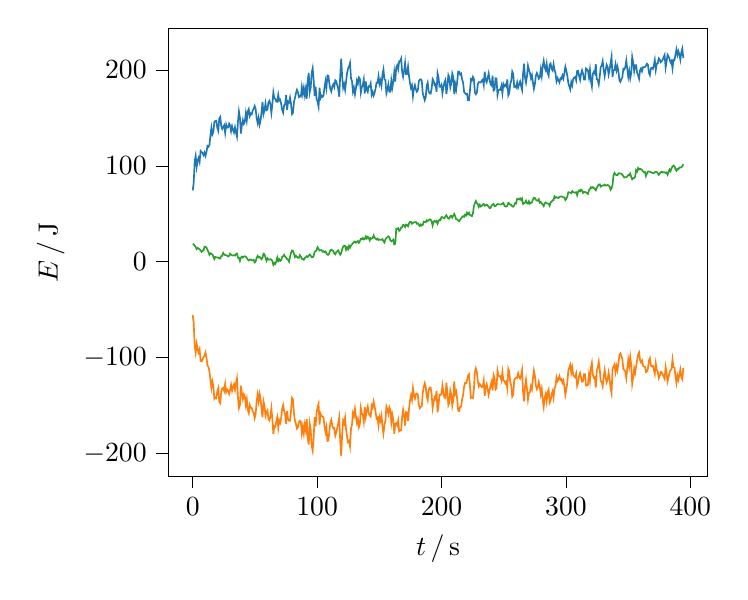
\begin{tikzpicture}

\definecolor{darkgray176}{RGB}{176,176,176}
\definecolor{darkorange25512714}{RGB}{255,127,14}
\definecolor{forestgreen4416044}{RGB}{44,160,44}
\definecolor{steelblue31119180}{RGB}{31,119,180}

\begin{axis}[
tick align=outside,
tick pos=left,
x grid style={darkgray176},
xlabel={\(\displaystyle t\,/\,\mathrm{s}\)},
xmin=-19.7179, xmax=414.0759,
xtick style={color=black},
y grid style={darkgray176},
ylabel={\(\displaystyle E\,/\,\mathrm{J}\)},
ymin=-224.2855, ymax=243.5555,
ytick style={color=black}
]
\addplot [semithick, steelblue31119180]
table {%
0 74.23
0.79 82.28
1.581 104.67
2.371 110.32
3.161 98.79
3.951 105.52
4.742 108.34
5.532 104.14
6.322 115.48
7.113 114.24
7.903 113.26
8.693 111.19
9.484 113.88
10.274 110.34
11.064 114.51
11.854 120.76
12.645 119.8
13.435 121.73
14.225 131.67
15.016 139.71
15.806 132.67
16.596 135.1
17.387 145.91
18.177 146.75
18.967 146.95
19.757 139.5
20.548 136.43
21.338 149.32
22.128 150.96
22.919 141.62
23.709 138.49
24.499 140.72
25.289 142.32
26.08 134.33
26.87 142.95
27.66 139.71
28.451 140.07
29.241 143.95
30.031 142.28
30.822 136.08
31.612 141.34
32.402 137.4
33.192 134.69
33.983 140.13
34.773 134.58
35.563 130.35
36.354 145.7
37.144 156.64
37.934 150.17
38.724 133.73
39.515 142.57
40.305 147.74
41.095 143.75
41.886 145.92
42.676 154.76
43.466 147.37
44.257 156.67
45.047 159.18
45.837 151.87
46.627 154.68
47.418 153.71
48.208 157.72
48.998 159.45
49.789 162.45
50.579 159.21
51.369 149.83
52.16 144.72
52.95 150.27
53.74 142.81
54.53 146.99
55.321 156.02
56.111 166.59
56.901 153.98
57.692 158.18
58.482 165.12
59.272 157.97
60.062 158.66
60.853 166.26
61.643 167.81
62.433 164.39
63.224 155.25
64.014 164.36
64.804 176.57
65.595 170.37
66.385 169.92
67.175 166.98
67.965 166.75
68.756 174.16
69.546 168.11
70.336 168.97
71.127 164.51
71.917 158.24
72.707 155.41
73.498 163.27
74.288 164.14
75.078 173.81
75.868 158.35
76.659 166.96
77.449 165.97
78.239 171.15
79.03 164.47
79.82 153.94
80.61 155.45
81.4 166.73
82.191 170.81
82.981 175.69
83.771 179.25
84.562 176.69
85.352 171.77
86.142 172.83
86.933 172.29
87.723 182.26
88.513 175.04
89.303 181.34
90.094 173.73
90.884 180.39
91.674 170.02
92.465 188.9
93.255 197
94.045 176.57
94.835 181.68
95.626 196.81
96.416 201.88
97.206 189.45
97.997 172.74
98.787 182.56
99.577 169.71
100.368 166.9
101.158 161.69
101.948 181.46
102.738 170.65
103.529 173.24
104.319 171.91
105.109 173.29
105.9 181.41
106.69 188.26
107.48 181.2
108.271 194.3
109.061 193.92
109.851 185.76
110.641 180.04
111.432 177.58
112.222 182.95
113.012 185.12
113.803 182.22
114.593 189.27
115.383 188.23
116.173 184.14
116.964 180.25
117.754 172.1
118.544 193.73
119.335 211.84
120.125 192.98
120.915 181.43
121.706 185.22
122.496 179.24
123.286 187.83
124.076 196.91
124.867 201.35
125.657 203.8
126.447 207.43
127.238 191.06
128.028 188.26
128.818 177.26
129.609 181.3
130.399 174.58
131.189 181.02
131.979 188.91
132.77 185.72
133.56 192.26
134.35 190.97
135.141 176.39
135.931 181.93
136.721 184.46
137.511 190.13
138.302 175.34
139.092 188.04
139.882 179.34
140.673 177.05
141.463 182.94
142.253 182.62
143.044 186.06
143.834 174.01
144.624 176.91
145.414 173.31
146.205 176.36
146.995 180.79
147.785 186.8
148.576 186.73
149.366 193.54
150.156 185.25
150.947 189
151.737 183.48
152.527 195.64
153.317 200.65
154.108 190.23
154.898 189.47
155.688 175.7
156.479 179.79
157.269 185.1
158.059 177.37
158.849 177.28
159.64 189.1
160.43 181.46
161.22 187.43
162.011 197.59
162.801 188.02
163.591 202.82
164.382 204.89
165.172 200.72
165.962 209.21
166.752 209.15
167.543 211.89
168.333 198.08
169.123 192.96
169.914 198.81
170.704 207.27
171.494 195.58
172.284 195.83
173.075 203.33
173.865 193.51
174.655 186.22
175.446 181.15
176.236 183.82
177.026 172.63
177.817 180.86
178.607 184.2
179.397 179.62
180.187 177.25
180.978 178.92
181.768 188.19
182.558 190.04
183.349 190.27
184.139 188.57
184.929 175.31
185.72 172.34
186.51 168.34
187.3 171.73
188.09 183.61
188.881 186.86
189.671 177.72
190.461 175.48
191.252 175.26
192.042 180.34
192.832 190.49
193.622 188.67
194.413 184.23
195.203 185.07
195.993 177.32
196.784 196.72
197.574 192.35
198.364 182.54
199.155 182.4
199.945 184.57
200.735 175.57
201.525 182.11
202.316 187.06
203.106 189.57
203.896 174.76
204.687 182.89
205.477 194.67
206.267 191.88
207.058 181.88
207.848 186.21
208.638 196.26
209.428 192.65
210.219 174.79
211.009 185.11
211.799 179.64
212.59 187.57
213.38 198.28
214.17 198.1
214.96 195.25
215.751 196.23
216.541 190.3
217.331 186.84
218.122 177.33
218.912 175.57
219.702 174.88
220.493 175.17
221.283 168.49
222.073 168.58
222.863 178.81
223.654 190.29
224.444 189.25
225.234 192.81
226.025 190.58
226.815 176.54
227.605 174.68
228.395 176.2
229.186 185.18
229.976 187.28
230.766 187.07
231.557 186.96
232.347 189.14
233.137 189.98
233.928 184.34
234.718 198.25
235.508 189.54
236.298 187.17
237.089 191.71
237.879 196.46
238.669 189.87
239.46 185.09
240.25 183.79
241.04 193.94
241.831 178.57
242.621 179.4
243.411 191.34
244.201 191.11
244.992 173.77
245.782 178.82
246.572 179.65
247.363 179.28
248.153 183.42
248.943 175.72
249.733 185.47
250.524 183.12
251.314 184.5
252.104 182.81
252.895 190.19
253.685 173.49
254.475 176.01
255.266 185.35
256.056 188.85
256.846 198.41
257.636 196.07
258.427 182.43
259.217 183.2
260.007 181.73
260.798 186.91
261.588 181.8
262.378 185.12
263.169 188.01
263.959 183.26
264.749 179.1
265.539 195.89
266.33 206.58
267.12 191.88
267.91 186.72
268.701 193.77
269.491 204.51
270.281 200.26
271.071 196.67
271.862 191.38
272.652 194.72
273.442 187.11
274.233 180.34
275.023 184.92
275.813 193.85
276.604 196.77
277.394 194.47
278.184 190.8
278.974 192.03
279.765 200.53
280.555 193.59
281.345 204.06
282.136 209.55
282.926 202.69
283.716 199.96
284.506 206.47
285.297 197.28
286.087 194.03
286.877 205.57
287.668 206.74
288.458 201.19
289.248 199.5
290.039 206.11
290.829 200.14
291.619 196.73
292.409 188.04
293.2 191.48
293.99 189.27
294.78 186.97
295.571 191.36
296.361 190.5
297.151 194.24
297.942 191.11
298.732 196.86
299.522 203.44
300.312 199.3
301.103 194.08
301.893 186.57
302.683 182.94
303.474 179.73
304.264 187.27
305.054 183.92
305.844 190.79
306.635 192.06
307.425 192.72
308.215 189.13
309.006 198.91
309.796 199.14
310.586 193.82
311.377 189.64
312.167 195.95
312.957 199.68
313.747 196.24
314.538 190.09
315.328 190.09
316.118 201.48
316.909 200.78
317.699 199.13
318.489 192.37
319.28 200.36
320.07 188.67
320.86 182.77
321.65 196.09
322.441 198.11
323.231 196.38
324.021 205.96
324.812 190.28
325.602 189.57
326.392 184.94
327.182 193.11
327.973 203.4
328.763 204.34
329.553 209.23
330.344 200.1
331.134 193.54
331.924 200.02
332.715 205.43
333.505 203.3
334.295 195.27
335.085 200.12
335.876 207.03
336.666 213.72
337.456 192.58
338.247 199.69
339.037 199.92
339.827 206.03
340.617 199.43
341.408 203.72
342.198 198.25
342.988 189.39
343.779 187.62
344.569 190.37
345.359 192.38
346.15 201.23
346.94 200.55
347.73 203.06
348.52 209.87
349.311 201.06
350.101 192.69
350.891 199.05
351.682 191.08
352.472 196.43
353.262 213.63
354.053 208.06
354.843 198.73
355.633 204.96
356.423 204.97
357.214 196.93
358.004 194.53
358.794 190.86
359.585 199.67
360.375 201.68
361.165 198.68
361.955 202.82
362.746 202.77
363.536 203.08
364.326 204.54
365.117 206.52
365.907 205.38
366.697 197.13
367.488 194.65
368.278 201.66
369.068 202.21
369.858 201.1
370.649 204.68
371.439 210.43
372.229 200.12
373.02 206.69
373.81 206.81
374.6 212.15
375.391 211.04
376.181 208.12
376.971 209.28
377.761 210.64
378.552 213.22
379.342 215.69
380.132 202.46
380.923 208.9
381.713 215.82
382.503 214.11
383.293 211.57
384.084 207.75
384.874 209.37
385.664 201.56
386.455 210.52
387.245 210.09
388.035 215.88
388.826 221.37
389.616 215.57
390.406 219.54
391.196 216.25
391.987 210.69
392.777 218.55
393.567 222.29
394.358 212.47
};
\addplot [semithick, darkorange25512714]
table {%
0 -55.64
0.79 -64.22
1.581 -88.02
2.371 -95.03
3.161 -85.66
3.951 -91.27
4.742 -94.79
5.532 -91.31
6.322 -103.62
7.113 -104.02
7.903 -102.08
8.693 -99.44
9.484 -98.28
10.274 -94.83
11.064 -100.05
11.854 -108.51
12.645 -109.94
13.435 -114.61
14.225 -122.96
15.016 -131.75
15.806 -124.99
16.596 -130.03
17.387 -143.25
18.177 -141.88
18.967 -142.51
19.757 -135.14
20.548 -132.05
21.338 -146.01
22.128 -147.66
22.919 -135.82
23.709 -132.49
24.499 -131.7
25.289 -134.86
26.08 -127.54
26.87 -136.18
27.66 -133.5
28.451 -134.71
29.241 -137.99
30.031 -133.97
30.822 -128.69
31.612 -134.94
32.402 -130.98
33.192 -128.01
33.983 -133.8
34.773 -126.75
35.563 -121.95
36.354 -141.71
37.144 -152.82
37.934 -149.45
38.724 -129.51
39.515 -137.29
40.305 -143.45
41.095 -138.59
41.886 -140.34
42.676 -149.54
43.466 -143.64
44.257 -154.53
45.047 -158.06
45.837 -149.59
46.627 -152.47
47.418 -152.56
48.208 -156.33
48.998 -157.58
49.789 -163.32
50.579 -159.14
51.369 -146.04
52.16 -138.69
52.95 -145.84
53.74 -137.97
54.53 -143.08
55.321 -153.53
56.111 -162.57
56.901 -145.75
57.692 -150.57
58.482 -160.84
59.272 -157.11
60.062 -155.28
60.853 -164.21
61.643 -165.66
62.433 -161.91
63.224 -153.06
64.014 -163.96
64.804 -179.9
65.595 -171.68
66.385 -172.34
67.175 -166.94
67.965 -162.43
68.756 -173.48
69.546 -165.59
70.336 -168.18
71.127 -163.15
71.917 -153.14
72.707 -149.66
73.498 -156.27
74.288 -159.2
75.078 -169.6
75.868 -155.82
76.659 -164.92
77.449 -165.97
78.239 -166.12
79.03 -155.31
79.82 -142.31
80.61 -144.18
81.4 -158.63
82.191 -166.1
82.981 -169.52
83.771 -174.23
84.562 -172.66
85.352 -167.84
86.142 -166.08
86.933 -167.07
87.723 -179.36
88.513 -172.17
89.303 -179.43
90.094 -169.9
90.884 -175.92
91.674 -164.32
92.465 -184.11
93.255 -190.89
94.045 -169.18
94.835 -175.4
95.626 -192.33
96.416 -197.34
97.206 -183.7
97.997 -162.44
98.787 -171.75
99.577 -157.92
100.368 -151.93
101.158 -148.37
101.948 -169.99
102.738 -158.69
103.529 -161.16
104.319 -161.56
105.109 -162.45
105.9 -171.59
106.69 -177.7
107.48 -172.55
108.271 -187.11
109.061 -186.8
109.851 -176.8
110.641 -168.07
111.432 -165.09
112.222 -171.24
113.012 -174.12
113.803 -173.79
114.593 -181.7
115.383 -178.3
116.173 -173.51
116.964 -168.59
117.754 -162.69
118.544 -186.58
119.335 -203.02
120.125 -180.16
120.915 -165.92
121.706 -168.71
122.496 -162.82
123.286 -175.48
124.076 -182.14
124.867 -188.37
125.657 -187.19
126.447 -192.83
127.238 -174.22
128.028 -170.26
128.818 -157.97
129.609 -161.01
130.399 -153.56
131.189 -161.29
131.979 -168.25
132.77 -164.22
133.56 -172.67
134.35 -169.58
135.141 -152.72
135.931 -158.49
136.721 -159.77
137.511 -167.08
138.302 -151.79
139.092 -161.89
139.882 -155.28
140.673 -151.19
141.463 -158
142.253 -160.49
143.044 -161.63
143.834 -150.03
144.624 -152.31
145.414 -145.92
146.205 -151.14
146.995 -156.82
147.785 -163.68
148.576 -162.77
149.366 -171.08
150.156 -162.2
150.947 -166.14
151.737 -160.78
152.527 -172.22
153.317 -179.48
154.108 -170.34
154.898 -166.09
155.688 -151.14
156.479 -154.23
157.269 -158.79
158.059 -151.95
158.849 -154.93
159.64 -167.89
160.43 -159.58
161.22 -164.58
162.011 -179.59
162.801 -169.31
163.591 -168.54
164.382 -170.85
165.172 -165.86
165.962 -177.04
166.752 -176.25
167.543 -176.19
168.333 -162.2
169.123 -154.61
169.914 -160.75
170.704 -171.03
171.494 -156.92
172.284 -157.61
173.075 -166.42
173.865 -153.67
174.655 -144.74
175.446 -139.65
176.236 -144.33
177.026 -132.19
177.817 -139.76
178.607 -143.01
179.397 -138.37
180.187 -137.69
180.978 -138.89
181.768 -149.95
182.558 -152.89
183.349 -151.45
184.139 -150.93
184.929 -137.07
185.72 -130.51
186.51 -126.76
187.3 -130.6
188.09 -140.42
188.881 -144.53
189.671 -134.55
190.461 -131.37
191.252 -131.39
192.042 -138.28
192.832 -152.77
193.622 -146.9
194.413 -141.76
195.203 -143.51
195.993 -134.9
196.784 -157.19
197.574 -150.22
198.364 -138.79
199.155 -139.15
199.945 -138.07
200.735 -129.23
201.525 -136.49
202.316 -141.81
203.106 -142.35
203.896 -126.3
204.687 -136.46
205.477 -149.76
206.267 -146.99
207.058 -134.35
207.848 -138.67
208.638 -150.32
209.428 -144.43
210.219 -125
211.009 -137.89
211.799 -135.43
212.59 -143.51
213.38 -155.42
214.17 -155.97
214.96 -151.59
215.751 -151.18
216.541 -143.73
217.331 -139.46
218.122 -130.65
218.912 -126.57
219.702 -126.79
220.493 -124.08
221.283 -119.09
222.073 -117.63
222.863 -130.19
223.654 -142.26
224.444 -141.78
225.234 -142.39
226.025 -132.65
226.815 -115.56
227.605 -111.43
228.395 -115.23
229.186 -125.05
229.976 -130.17
230.766 -127.76
231.557 -129.46
232.347 -130.98
233.137 -130.49
233.928 -124.12
234.718 -139.92
235.508 -130.72
236.298 -127.66
237.089 -133.26
237.879 -139.08
238.669 -134.07
239.46 -129.04
240.25 -125.44
241.04 -134.41
241.831 -118.37
242.621 -121.57
243.411 -133.38
244.201 -132.04
244.992 -113.69
245.782 -118.95
246.572 -119.94
247.363 -119.57
248.153 -123.65
248.943 -115.15
249.733 -124.25
250.524 -124.45
251.314 -127.1
252.104 -125.37
252.895 -132.07
253.685 -112.09
254.475 -115.2
255.266 -126.04
256.056 -129.55
256.846 -140.83
257.636 -138.78
258.427 -123.69
259.217 -121.98
260.007 -121.03
260.798 -121.28
261.588 -116.49
262.378 -120.29
263.169 -121.98
263.959 -118.94
264.749 -113.28
265.539 -135.8
266.33 -145.78
267.12 -130.22
267.91 -123.11
268.701 -132.98
269.491 -144.03
270.281 -137.26
271.071 -136.15
271.862 -129.96
272.652 -133.18
273.442 -122.46
274.233 -113.72
275.023 -118.57
275.813 -129.09
276.604 -132.99
277.394 -130.92
278.184 -125.71
278.974 -130.55
279.765 -138.37
280.555 -132.77
281.345 -144.43
282.136 -151.66
282.926 -141.87
283.716 -138.2
284.506 -145.66
285.297 -136.53
286.087 -133.69
286.877 -147.25
287.668 -144.97
288.458 -138.91
289.248 -135.44
290.039 -141.91
290.829 -132.05
291.619 -130.09
292.409 -120.82
293.2 -124.79
293.99 -122.83
294.78 -119.44
295.571 -123.49
296.361 -122.56
297.151 -126.47
297.942 -124.03
298.732 -129.89
299.522 -139.16
300.312 -133.64
301.103 -126.23
301.893 -114.22
302.683 -110.62
303.474 -107.76
304.264 -115.83
305.054 -110.39
305.844 -118.41
306.635 -119.77
307.425 -120.77
308.215 -116.77
309.006 -129.65
309.796 -126.23
310.586 -119.53
311.377 -116.33
312.167 -120.9
312.957 -125.29
313.747 -124.65
314.538 -117.42
315.328 -117.49
316.118 -129.18
316.909 -129.36
317.699 -128.47
318.489 -117.8
319.28 -124.66
320.07 -110.99
320.86 -105.84
321.65 -118.28
322.441 -121.29
323.231 -120.7
324.021 -131.51
324.812 -113.31
325.602 -110.67
326.392 -104.45
327.182 -112.48
327.973 -125.09
328.763 -125.34
329.553 -129.9
330.344 -120.59
331.134 -113.08
331.924 -120.61
332.715 -126.09
333.505 -123.29
334.295 -115.97
335.085 -121.94
335.876 -132.07
336.666 -137.3
337.456 -112.42
338.247 -109.7
339.037 -107.34
339.827 -115.28
340.617 -109.02
341.408 -113.43
342.198 -106.2
342.988 -97.08
343.779 -95.78
344.569 -98.67
345.359 -101.67
346.15 -112.18
346.94 -112.82
347.73 -114.93
348.52 -121.71
349.311 -112.06
350.101 -102.29
350.891 -109.09
351.682 -99.19
352.472 -107.93
353.262 -127.73
354.053 -120.98
354.843 -111.57
355.633 -116.24
356.423 -109.51
357.214 -102.9
358.004 -96.88
358.794 -94.72
359.585 -102.83
360.375 -105.19
361.165 -103.08
361.955 -108.61
362.746 -109.62
363.536 -109.62
364.326 -115.3
365.117 -114.65
365.907 -111.56
366.697 -103.13
367.488 -100.7
368.278 -108.38
369.068 -109.37
369.858 -108.73
370.649 -112.28
371.439 -117.16
372.229 -106.31
373.02 -113.12
373.81 -114.58
374.6 -121.56
375.391 -119.04
376.181 -115.07
376.971 -115.42
377.761 -117.57
378.552 -119.9
379.342 -122.39
380.132 -109.94
380.923 -115.92
381.713 -125.12
382.503 -120.71
383.293 -115.51
384.084 -113.27
384.874 -112.2
385.664 -102.2
386.455 -110.31
387.245 -110.62
388.035 -119.42
388.826 -126.53
389.616 -118.87
390.406 -123.2
391.196 -117.99
391.987 -112.53
392.777 -120.25
393.567 -122.68
394.358 -110.88
};
\addplot [semithick, forestgreen4416044]
table {%
0 18.58
0.79 18.06
1.581 16.65
2.371 15.29
3.161 13.13
3.951 14.25
4.742 13.55
5.532 12.83
6.322 11.87
7.113 10.21
7.903 11.17
8.693 11.75
9.484 15.6
10.274 15.52
11.064 14.46
11.854 12.26
12.645 9.86
13.435 7.12
14.225 8.71
15.016 7.96
15.806 7.67
16.596 5.07
17.387 2.66
18.177 4.87
18.967 4.44
19.757 4.37
20.548 4.38
21.338 3.32
22.128 3.3
22.919 5.8
23.709 6
24.499 9.02
25.289 7.45
26.08 6.79
26.87 6.77
27.66 6.21
28.451 5.36
29.241 5.96
30.031 8.31
30.822 7.39
31.612 6.4
32.402 6.42
33.192 6.68
33.983 6.33
34.773 7.83
35.563 8.4
36.354 3.99
37.144 3.82
37.934 0.72
38.724 4.23
39.515 5.28
40.305 4.29
41.095 5.16
41.886 5.59
42.676 5.22
43.466 3.73
44.257 2.14
45.047 1.12
45.837 2.28
46.627 2.2
47.418 1.14
48.208 1.39
48.998 1.88
49.789 -0.87
50.579 0.06
51.369 3.79
52.16 6.03
52.95 4.44
53.74 4.84
54.53 3.91
55.321 2.49
56.111 4.03
56.901 8.23
57.692 7.62
58.482 4.28
59.272 0.86
60.062 3.38
60.853 2.05
61.643 2.15
62.433 2.48
63.224 2.19
64.014 0.4
64.804 -3.33
65.595 -1.31
66.385 -2.43
67.175 0.04
67.965 4.31
68.756 0.68
69.546 2.53
70.336 0.79
71.127 1.36
71.917 5.1
72.707 5.75
73.498 7
74.288 4.94
75.078 4.21
75.868 2.53
76.659 2.04
77.449 0
78.239 5.04
79.03 9.16
79.82 11.64
80.61 11.28
81.4 8.1
82.191 4.72
82.981 6.17
83.771 5.02
84.562 4.03
85.352 3.93
86.142 6.75
86.933 5.21
87.723 2.9
88.513 2.87
89.303 1.91
90.094 3.83
90.884 4.48
91.674 5.7
92.465 4.8
93.255 6.1
94.045 7.38
94.835 6.28
95.626 4.48
96.416 4.54
97.206 5.76
97.997 10.3
98.787 10.81
99.577 11.78
100.368 14.97
101.158 13.32
101.948 11.47
102.738 11.95
103.529 12.07
104.319 10.35
105.109 10.84
105.9 9.82
106.69 10.56
107.48 8.66
108.271 7.19
109.061 7.12
109.851 8.96
110.641 11.97
111.432 12.5
112.222 11.71
113.012 11
113.803 8.42
114.593 7.57
115.383 9.93
116.173 10.63
116.964 11.67
117.754 9.41
118.544 7.14
119.335 8.82
120.125 12.82
120.915 15.51
121.706 16.51
122.496 16.41
123.286 12.36
124.076 14.77
124.867 12.98
125.657 16.61
126.447 14.6
127.238 16.84
128.028 18
128.818 19.29
129.609 20.29
130.399 21.02
131.189 19.74
131.979 20.67
132.77 21.5
133.56 19.59
134.35 21.39
135.141 23.67
135.931 23.44
136.721 24.7
137.511 23.06
138.302 23.55
139.092 26.14
139.882 24.06
140.673 25.86
141.463 24.94
142.253 22.13
143.044 24.43
143.834 23.98
144.624 24.6
145.414 27.39
146.205 25.22
146.995 23.97
147.785 23.12
148.576 23.96
149.366 22.46
150.156 23.05
150.947 22.86
151.737 22.7
152.527 23.42
153.317 21.18
154.108 19.89
154.898 23.38
155.688 24.56
156.479 25.56
157.269 26.31
158.059 25.42
158.849 22.35
159.64 21.2
160.43 21.88
161.22 22.85
162.011 18
162.801 18.71
163.591 34.28
164.382 34.04
165.172 34.86
165.962 32.17
166.752 32.9
167.543 35.7
168.333 35.89
169.123 38.35
169.914 38.05
170.704 36.25
171.494 38.67
172.284 38.22
173.075 36.91
173.865 39.84
174.655 41.48
175.446 41.5
176.236 39.5
177.026 40.43
177.817 41.1
178.607 41.19
179.397 41.25
180.187 39.56
180.978 40.03
181.768 38.24
182.558 37.15
183.349 38.82
184.139 37.65
184.929 38.25
185.72 41.83
186.51 41.58
187.3 41.13
188.09 43.2
188.881 42.33
189.671 43.17
190.461 44.11
191.252 43.88
192.042 42.05
192.832 37.72
193.622 41.77
194.413 42.47
195.203 41.56
195.993 42.42
196.784 39.52
197.574 42.13
198.364 43.75
199.155 43.25
199.945 46.5
200.735 46.35
201.525 45.62
202.316 45.25
203.106 47.23
203.896 48.45
204.687 46.43
205.477 44.91
206.267 44.89
207.058 47.52
207.848 47.53
208.638 45.94
209.428 48.22
210.219 49.8
211.009 47.22
211.799 44.2
212.59 44.06
213.38 42.86
214.17 42.13
214.96 43.67
215.751 45.05
216.541 46.58
217.331 47.38
218.122 46.68
218.912 49
219.702 48.09
220.493 51.09
221.283 49.39
222.073 50.95
222.863 48.61
223.654 48.03
224.444 47.47
225.234 50.42
226.025 57.93
226.815 60.97
227.605 63.26
228.395 60.97
229.186 60.13
229.976 57.1
230.766 59.31
231.557 57.51
232.347 58.16
233.137 59.49
233.928 60.22
234.718 58.33
235.508 58.82
236.298 59.51
237.089 58.45
237.879 57.39
238.669 55.8
239.46 56.05
240.25 58.34
241.04 59.53
241.831 60.2
242.621 57.83
243.411 57.95
244.201 59.07
244.992 60.08
245.782 59.87
246.572 59.71
247.363 59.71
248.153 59.77
248.943 60.58
249.733 61.22
250.524 58.66
251.314 57.4
252.104 57.45
252.895 58.12
253.685 61.4
254.475 60.8
255.266 59.3
256.056 59.3
256.846 57.58
257.636 57.28
258.427 58.74
259.217 61.22
260.007 60.7
260.798 65.63
261.588 65.31
262.378 64.83
263.169 66.03
263.959 64.32
264.749 65.82
265.539 60.09
266.33 60.8
267.12 61.66
267.91 63.62
268.701 60.79
269.491 60.48
270.281 63.01
271.071 60.52
271.862 61.42
272.652 61.54
273.442 64.66
274.233 66.63
275.023 66.35
275.813 64.76
276.604 63.78
277.394 63.55
278.184 65.09
278.974 61.48
279.765 62.16
280.555 60.83
281.345 59.63
282.136 57.89
282.926 60.81
283.716 61.77
284.506 60.82
285.297 60.75
286.087 60.34
286.877 58.32
287.668 61.78
288.458 62.28
289.248 64.05
290.039 64.2
290.829 68.08
291.619 66.64
292.409 67.23
293.2 66.69
293.99 66.44
294.78 67.52
295.571 67.87
296.361 67.94
297.151 67.76
297.942 67.09
298.732 66.97
299.522 64.28
300.312 65.66
301.103 67.85
301.893 72.34
302.683 72.32
303.474 71.97
304.264 71.43
305.054 73.53
305.844 72.38
306.635 72.29
307.425 71.95
308.215 72.37
309.006 69.26
309.796 72.9
310.586 74.3
311.377 73.31
312.167 75.05
312.957 74.39
313.747 71.6
314.538 72.68
315.328 72.6
316.118 72.3
316.909 71.42
317.699 70.66
318.489 74.57
319.28 75.7
320.07 77.68
320.86 76.93
321.65 77.81
322.441 76.82
323.231 75.68
324.021 74.44
324.812 76.96
325.602 78.9
326.392 80.49
327.182 80.63
327.973 78.31
328.763 79
329.553 79.33
330.344 79.51
331.134 80.45
331.924 79.41
332.715 79.34
333.505 80
334.295 79.3
335.085 78.18
335.876 74.96
336.666 76.43
337.456 80.15
338.247 89.99
339.037 92.58
339.827 90.75
340.617 90.41
341.408 90.28
342.198 92.05
342.988 92.3
343.779 91.84
344.569 91.69
345.359 90.71
346.15 89.05
346.94 87.73
347.73 88.13
348.52 88.16
349.311 89
350.101 90.41
350.891 89.96
351.682 91.9
352.472 88.5
353.262 85.9
354.053 87.07
354.843 87.16
355.633 88.72
356.423 95.46
357.214 94.03
358.004 97.64
358.794 96.15
359.585 96.85
360.375 96.49
361.165 95.6
361.955 94.21
362.746 93.16
363.536 93.45
364.326 89.24
365.117 91.87
365.907 93.82
366.697 94
367.488 93.94
368.278 93.28
369.068 92.84
369.858 92.37
370.649 92.41
371.439 93.27
372.229 93.81
373.02 93.57
373.81 92.23
374.6 90.59
375.391 92
376.181 93.04
376.971 93.86
377.761 93.07
378.552 93.32
379.342 93.31
380.132 92.52
380.923 92.99
381.713 90.7
382.503 93.4
383.293 96.07
384.084 94.49
384.874 97.17
385.664 99.36
386.455 100.22
387.245 99.48
388.035 96.46
388.826 94.84
389.616 96.7
390.406 96.34
391.196 98.26
391.987 98.16
392.777 98.3
393.567 99.6
394.358 101.59
};
\end{axis}

\end{tikzpicture}

            \end{adjustbox}
            \caption{\(\delta t^*=0.19\)}
        \end{subfigure}%
        \caption{A plot of the computed kinetic energy (blue), potential energy (orange) and total energy (green) of a Lennard-Jones fluid with 100 particles using times steps \(0.001,0.05\) and \(0.19\) in reduced time units. 5000 steps are used for each run. A significant energy drift occurred for \(\delta t^*=0.19\), suggesting that this time step is too large.}
    \end{figure}

    \subsection{Radial Distribution Function}
    As we commented above, due to the high number density of atoms and strong interactions, liquid often exhibits short-range order. This can be captured by the \textit{spatial autocorrelation function}
    \begin{equation}
        g(\vb{r}_1,\vb{r}_2)\coloneqq\frac{1}{n_0^2}\eval{n(\vb{r}_1)n(\vb{r}_2)}
    \end{equation}
    where \(n_0=N/V\) is the average particle density, just like the velocity autocorrelation function you met in Part II Statistical Mechanics. In an isotropic, homogeneous medium, the autocorrelation function should be only dependent on the particle distance \(r=\norm{\vb{r}_1-\vb{r}_2}\), and so it allows us to define the \textit{radial distribution function}
    \begin{equation}
        g(r)=\frac{\eval{n(r)}}{n_0}\,.
    \end{equation}
    This can be understood as a histogram of two-particle distances, which can be constructed by going through the following steps:
    \begin{enumerate}[topsep=0pt]
        \item Pick a reference particle \(i\) at position \(\vb{r}_i\).
        \item Draw a spherical shell of radius \(r\) and thickness \(\Delta r\) centred at \(\vb{r}_i\). Determine the number of particles in the shell, which we denote as \(n_i(r,\Delta r)\). A particle \(j\) in this shell would satisfy
        \begin{equation}
            r\le \norm{\vb{r}_i-\vb{r}_j}<r+\Delta r\,.
        \end{equation}

        A small \(\Delta r\) will give us a high resolution, but it will introduce noise. A large \(r\) will smooth the distribution function, but we may lose some of the structural details.
        \item Divide \(n_i(r,\Delta r)\) by the volume of the shell to convert it into a number density, and average over reference particles.
        \begin{equation}
            \bar{\rho}(r,\Delta r)=\frac{1}{N}\sum_{i=1}^{N}\frac{n_i(r,\Delta r)}{4\pi r^2\Delta r}\,,
        \end{equation}
        where we assumed \(\Delta r\ll r\).
        \item Normalise this quantity by the particle number density of \(\rho=(N-1)/V\)
        \begin{equation}\label{radial_distribution_function}
            g(r)=\frac{\bar{\rho}(r,\Delta r)}{\rho}=\frac{V}{4\pi r^2\Delta r N(N-1)}\sum_{i}^{N}n_i(r,\Delta r)\,.
        \end{equation}
        The resulting \(g(r)\) is a dimensionless quantity. Note that we use \(N-1\) because we do not consider a particle correlating with itself, although for large \(N\), we can replace \(N-1\) by \(N\).
    \end{enumerate}

    A \(g(r)>1\) at some \(r\) would mean that we have an enhanced probability of meeting another particle at distance \(r\) away from one particle, and \(g(r)<1\) means that there is a depletion region.

    \begin{figure}
        \centering
        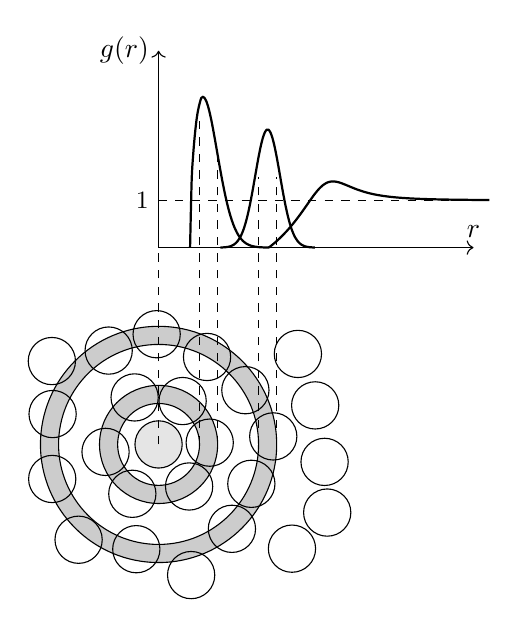
\begin{tikzpicture}
            \draw[fill=gray!40] (0,0) circle (1.5);
            \draw[fill=white] (0,0) circle (1.27);
            \draw[fill=gray!40] (0,0) circle (0.75);
            \draw[fill=white] (0,0) circle (0.52);
            \draw[fill=gray!20] (0,0) circle (0.3);
            \draw (2:0.65) circle (0.3);
            \draw (61:0.63) circle (0.3);
            \draw (117:0.67) circle (0.3);
            \draw (188:0.68) circle (0.3);
            \draw (242:0.71) circle (0.3);
            \draw (306:0.66) circle (0.3);
            \draw (32:1.3) circle (0.3);
            \draw (61:1.27) circle (0.3);
            \draw (91:1.4) circle (0.3);
            \draw (118:1.35) circle (0.3);
            \draw (142:1.72) circle (0.3);
            \draw (164:1.4) circle (0.3);
            \draw (198:1.42) circle (0.3);
            \draw (230:1.58) circle (0.3);
            \draw (258:1.36) circle (0.3);
            \draw (284:1.71) circle (0.3);
            \draw (311:1.42) circle (0.3);
            \draw (337:1.28) circle (0.3);
            \draw (4:1.46) circle (0.3);
            \draw (14:2.05) circle (0.3);
            \draw (33:2.11) circle (0.3);
            \draw (-6:2.12) circle (0.3);
            \draw (-22:2.31) circle (0.3);
            \draw (-38:2.15) circle (0.3);
            \draw[dashed] (0,0)--(0,2.5);
            \draw[dashed] (0.52,0)--(0.52,4.2);
            \draw[dashed] (0.75,0)--(0.75,3.7);
            \draw[dashed] (1.27,0)--(1.27,3.4);
            \draw[dashed] (1.5,0)--(1.5,3.4);
            \draw[->] (0,2.5)--(4,2.5)node[above]{\(r\)};
            \draw[->] (0,2.5)--(0,5)node[left]{\(g(r)\)};
            \draw[dashed] (0,3.1)node[left]{\small\(1\)}--(4,3.1);
            \draw[thick,domain=0:1, smooth, variable=\x,samples=50] plot ({\x+0.4}, {2.5+6*2.72^(-9*\x*\x)*(\x^0.5)});
            \draw[thick,domain=-0.6:0.6, smooth, variable=\x,samples=50] plot ({\x+1.385}, {2.5+1.5*2.72^(-20*\x*\x)});
            \draw[thick,domain=0:3.5, smooth, variable=\x,samples=50] plot ({0.8*\x+1.4}, {2.5+0.6*(\x*\x*\x*\x*\x*\x+0.8*\x*\x+\x)/(\x*\x*\x*\x*\x*\x+1)});
        \end{tikzpicture}
        \caption{A typical radial distribution function of liquid. \(g(r)=0\) for small \(r\) due to hard-core repulsion. There are several peaks with \(g(r)>1\) at intermediate range, corresponding to the first, second and higher coordination shells. At large \(r\), \(g(r)\to 1\) as the distribution of particles become decorrelated.}
        \label{Fig:RDF}
    \end{figure}

    A schematic construction of the radial distribution function for a 2D Lennard-Jones fluid is shown in \cref{Fig:RDF}. For distances \(r\ll \sigma\), where \(\sigma\) is the repulsive core diameter, the radial distribution \(\to 0\) because particles are excluded from this region. The maximum at a distance little over \(\sigma\) reflects the well defined coordination shell of nearest neighbours around a particle in a liquid. This peak in \(g(r)\) is characteristic for the high density prevalent in liquids and is absent in the vapour phase. In most liquids there is also a broader second nearest neighbour peak. As a result of the disorder in liquids, this structure is considerably less pronounced compared to solids. For distances larger than second neighbours, fluctuations gradually takes over and the distribution of atoms becomes homogeneous, with \(g(r)\to 1\).

    As for a comparison, a crystalline solid has long-range order extending to infinity, so the radial distribution function should have well defined peaks extending to infinity (ideally) except being broadened by thermal vibrations at non-zero temperatures.

    \begin{figure}
        \centering
        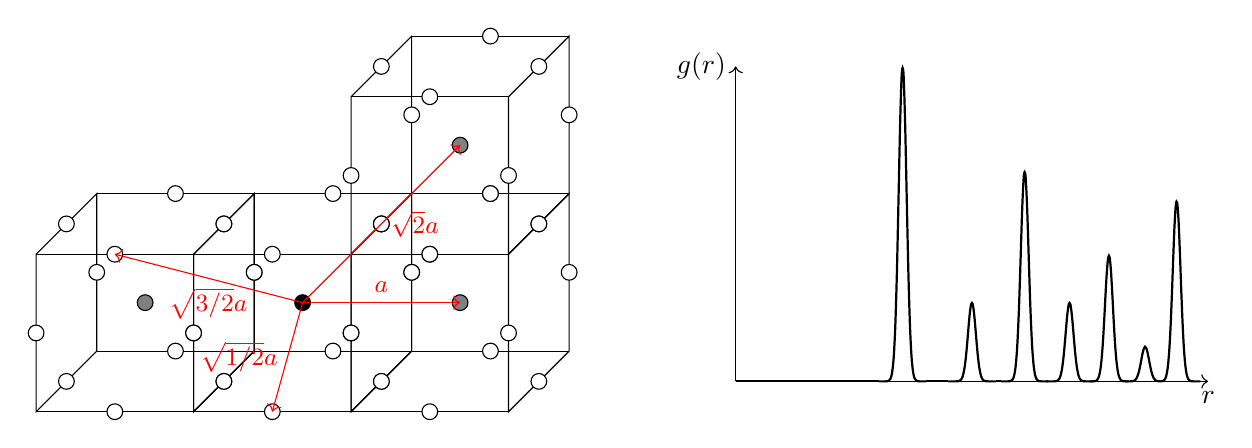
\begin{tikzpicture}
            \draw[fill=black] (0,0) circle (0.1);
            \draw (-1,-1,-1)--(-1,-1,1)--(-1,1,1)--(-1,1,-1)--(-1,-1,-1);
            \draw (1,-1,-1)--(1,-1,1)--(1,1,1)--(1,1,-1)--(1,-1,-1);
            \draw (-1,1,1)--(1,1,1);
            \draw (-1,1,-1)--(1,1,-1);
            \draw (-1,-1,1)--(1,-1,1);
            \draw (-1,-1,-1)--(1,-1,-1);
            \foreach \i in {-1,1}{
                \foreach \j in {-1,1}{
                    \draw[fill=white] (\i,0,\j) circle (0.1);
                    \draw[fill=white] (0.5*\i+0.5*\j,1,0.5*\i-0.5*\j) circle (0.1);
                    \draw[fill=white] (0.5*\i+0.5*\j,-1,0.5*\i-0.5*\j) circle (0.1);
                }
            }
            \foreach \l in {-2,2}{
                \begin{scope}[shift={(\l,0,0)}]
                    \draw[fill=gray] (0,0) circle (0.1);
                    \draw (-1,-1,-1)--(-1,-1,1)--(-1,1,1)--(-1,1,-1)--(-1,-1,-1);
                    \draw (1,-1,-1)--(1,-1,1)--(1,1,1)--(1,1,-1)--(1,-1,-1);
                    \draw (-1,1,1)--(1,1,1);
                    \draw (-1,1,-1)--(1,1,-1);
                    \draw (-1,-1,1)--(1,-1,1);
                    \draw (-1,-1,-1)--(1,-1,-1);
                    \foreach \i in {-1,1}{
                        \foreach \j in {-1,1}{
                            \draw[fill=white] (\i,0,\j) circle (0.1);
                            \draw[fill=white] (0.5*\i+0.5*\j,1,0.5*\i-0.5*\j) circle (0.1);
                            \draw[fill=white] (0.5*\i+0.5*\j,-1,0.5*\i-0.5*\j) circle (0.1);
                        }
                    }
                \end{scope}
            }
            \begin{scope}[shift={(2,2,0)}]
                \draw[fill=gray] (0,0) circle (0.1);
                \draw (-1,-1,-1)--(-1,-1,1)--(-1,1,1)--(-1,1,-1)--(-1,-1,-1);
                \draw (1,-1,-1)--(1,-1,1)--(1,1,1)--(1,1,-1)--(1,-1,-1);
                \draw (-1,1,1)--(1,1,1);
                \draw (-1,1,-1)--(1,1,-1);
                \draw (-1,-1,1)--(1,-1,1);
                \draw (-1,-1,-1)--(1,-1,-1);
                \foreach \i in {-1,1}{
                    \foreach \j in {-1,1}{
                        \draw[fill=white] (\i,0,\j) circle (0.1);
                        \draw[fill=white] (0.5*\i+0.5*\j,1,0.5*\i-0.5*\j) circle (0.1);
                        \draw[fill=white] (0.5*\i+0.5*\j,-1,0.5*\i-0.5*\j) circle (0.1);
                    }
                }
            \end{scope}
            \draw[->,red] (0,0,0)--node[left]{\small\(\sqrt{1/2}a\)}(0,-1,1);
            \draw[->,red] (0,0,0)--node[above]{\small\(a\)}(2,0,0);
            \draw[->,red] (0,0,0)--node[below]{\small\(\sqrt{3/2}a\)}(-2,1,1);
            \draw[->,red] (0,0,0)--node[right]{\small\(\sqrt{2}a\)}(2,2,0);
            \begin{scope}[shift={(5.5,-1)}]
                \draw[->] (0,0)--(6,0)node[below]{\(r\)};
                \draw[->] (0,0)--(0,4)node[left]{\(g(r)\)};
                \draw[thick] (0,0)--(1.82,0);
                \draw[thick] (2.42,0)--(2.7,0);
                \draw[thick] (3.3,0)--(3.37,0);
                \draw[thick,domain=-0.3:0.3, smooth, variable=\x,samples=30] plot ({\x+2.12}, {4*2.72^(-200*\x*\x)});
                \draw[thick,domain=-0.3:0.3, smooth, variable=\x,samples=30] plot ({\x+3}, {1*2.72^(-200*\x*\x)});
                \draw[thick,domain=-0.3:0.3, smooth, variable=\x,samples=30] plot ({\x+3.67}, {2.67*2.72^(-200*\x*\x)});
                \draw[thick,domain=-0.3:0.3, smooth, variable=\x,samples=30] plot ({\x+4.24}, {1*2.72^(-200*\x*\x)});
                \draw[thick,domain=-0.25:0.25, smooth, variable=\x,samples=30] plot ({\x+4.74}, {1.6*2.72^(-200*\x*\x)});
                \draw[thick,domain=-0.25:0.2, smooth, variable=\x,samples=30] plot ({\x+5.2}, {0.44*2.72^(-200*\x*\x)});
                \draw[thick,domain=-0.2:0.3, smooth, variable=\x,samples=30] plot ({\x+5.6}, {2.29*2.72^(-200*\x*\x)});
            \end{scope}
        \end{tikzpicture}
        \caption{Radial distribution function in a solid fcc crystal.}
    \end{figure}
    
    \subsubsection{Coordination Numbers}
    As suggested by \cref{Fig:RDF} the integral of the first peak of RDF is related to the average number of particles \(n_c\) in the first coordination shell, which is also known as the \textit{coordination number}. In order to measure \(n_c\) we must specify how close an atom must approach the central particle in order to be counted as a first neighbour. The position \(r_{\text{min}}\) of the minimum between the first and second maximum is used as a common (but not unique) criterion to define the first coordination shell. \(n_c\) is then found from the integral (for three dimensional cases)
    \begin{equation}
        n_c=4\pi\rho\int_{0}^{r_c}\dd{r}r^2g(r)\,,
    \end{equation}
    with \(r_c=r_{\text{min}}\) in our cases.
    \subsubsection{Radial Distribution Function in Statistical Mechanics}
    The way we introduced the radial distribution function was operational in the sense that it is based on how this quantity is determined in a simulation. We will now give a proper statistical mechanical definition of the radial distribution function making use of the Dirac delta function. We first consider a more general pair correlation function which not only probes the distance \(r\) between particles but also the orientation of the displacement vector \(\vb{r}\).
    \begin{equation}\label{pair_correlation_function}
        \gamma(\vb{r})=\frac{V}{N(N-1)}\eval{\sum_{i,j\ne i}^{N}\delta(\vb{r}_{ij}-\vb{r})}\,,
    \end{equation}
    where the angular bracket denote an integral over the configurational probability distribution function (\ref{configuration_integral}). In a more explicit form,
    \begin{equation}
        \gamma(\vb{r})=\frac{V}{N(N-1)}\sum_{i,j\ne i}^{N}\int\dd[3N]{\vb{r}^N}P_N(\vb{r}^N)\delta(\vb{r}_{ij}-\vb{r})\,.
    \end{equation}
    It is proportional to the probability of observing two particles separated by a vector \(\vb{r}\). This correlation function with the information on the orientation of \(\vb{r}\) included is suitable for crystalline solids, in which the lattice defines special directions in space. Liquids are isotropic systems with no preference for a direction, so we expect the function \(\gamma(\vb{r})\) to depend only on the length \(r=\norm{\vb{r}}\). Using this property, we integrate over a spherical shell \(V(r,\Delta r)\) with radius between \(r\) and \(r+\Delta r\), and assuming that the shell is sufficiently thin, we then write
    \begin{equation}
        \int_{V(r,\Delta r)}\dd[3]{\vb{r}}\gamma(\vb{r})\approx 4\pi r^2\Delta r g(r)\,.
    \end{equation}
    Here the \(g(r)\) is the radial distribution function. Substituting the expression of \(\gamma(\vb{r})\), we get
    \begin{align}
        g(r)&\approx\frac{V}{4\pi r^2\Delta r N(N-1)}\int_{V(r,\Delta r)}\dd[3]{\vb{r}}\sum_{i,j\ne i}\int\dd[3N]{\vb{r}^N}P_N(\vb{r}^N)\delta(\vb{r}_{ij}-\vb{r})\notag \\
        &=\frac{V}{4\pi r^2\Delta r N(N-1)}\int\dd[3N]{\vb{r}^N}P_N(\vb{r}^N)\sum_{i,j\ne i}\int_{V(r,\Delta r)}\dd[3]{\vb{r}}\delta(\vb{r}_{ij}-\vb{r})\,,
    \end{align}
    where we have changed the order of integration. The inner integral gives unity when the vector \(\vb{r}_{ij}=\vb{r}_i-\vb{r}_j\) lies within volume \(V(r,\Delta r)\) and zero otherwise. The delta function therefore counts the number of particle pairs with distances between \(r\) and \(r+\Delta r\). Taking particle \(i\) as reference we recover the quantity \(n_i(r,\Delta r)\) introduced before
    \begin{equation}
        n_i(r,\Delta r)=\sum_{j\ne i}\int_{V(r,\Delta r)}\dd[3]{\vb{r}}\delta(\vb{r}_{ij}-\vb{r})\,.
    \end{equation}
    Therefore,
    \begin{align}
        g(r)&\approx\frac{V}{4\pi r^2\Delta r N(N-1)}\int\dd[3N]{\vb{r}^N}P_N(\vb{r}^N)\sum_i n_i(r,\Delta r)\notag\\
        &=\frac{V}{4\pi r^2\Delta r N(N-1)}\eval{\sum_i n_i(r,\Delta r)}\,.
    \end{align}
    This becomes an equality in the limit of an infinitely thin shell,
    \begin{equation}
        g(r)=\lim_{\Delta r\to 0}\frac{V}{4\pi r^2\Delta r N(N-1)}\eval{\sum_i n_i(r,\Delta r)}\,.
    \end{equation}
    Since all particles are equivalent, we must have
    \begin{equation}
        g(r)=\frac{V}{N-1}\lim_{\Delta r\to 0}\frac{1}{4\pi r^2\Delta r}\eval{n(r,\Delta r)}\,,
    \end{equation}
    where we removed the subscript \(i\) to indicate a generic particle. We identify this linked to our instantaneous, histogramic radial distribution function (\ref{radial_distribution_function}) via
    \begin{equation}
        g_{\text{stat}}(r)=\frac{N-1}{N}g_{\text{hist}}(r)\,,
    \end{equation}
    where \((N-1)/N\) is a good approximation to \(1\) except at very low density. We could have avoided this complexity if we used \(N^2\) as the normalisation factor in the definition of pair correlation function (\ref{pair_correlation_function}), but it turns out that \(N(N-1)\) is the correct normalisation factor for a good treatment at very low density, i.e. in a gas phase limit. Consider a system with only two particles (\(N=2\)) in a finite volume \(V\),
    \begin{align}
        \gamma(\vb{r})&=\frac{V}{N(N-1)}\eval{\sum_{i,j\ne i}\delta(\vb{r}_{ij}-\vb{r})}=V\eval{\delta(\vb{r}_{ij}-\vb{r})}\notag \\
        &=V\int\dd[3]{\vb{r}_1}\dd[3]{\vb{r}_2}P_2(\vb{r}_1,\vb{r}_2)\delta(\vb{r}_{12}-\vb{r})\,.
    \end{align}
    \(P_2\) is just the Boltzmann exponent of the pair potential, and so
    \begin{equation}
        \gamma(\vb{r})=V\frac{\int\dd[3]{\vb{r}_1}\dd[3]{\vb{r}_2}\exp[-V(r_{12})/k_B T]\delta(\vb{r}_{12}-\vb{r})}{\int\dd[3]{\vb{r}_1}\dd[3]{\vb{r}_2}\exp[-V(r_{12})/k_B T]}\,.
    \end{equation}
    Transforming to the CoM coordinate \(\vb{r}\) and relative coordinate \(\vb{r}'=\vb{r}_{12}\) gives
    \begin{equation}
        \gamma(\vb{r})=V\frac{\int\dd[3]{\vb{R}}\dd[3]{\vb{r}'}\exp[-V(r'_{12})/k_B T]\delta(\vb{r}'-\vb{r})}{\int\dd[3]{\vb{R}}\dd[3]{\vb{r}'}\exp[-V(r'_{12})/k_B T]}\,.
    \end{equation}
    Since the potential is independent of \(\vb{R}\), the integral over \(\vb{R}\) gives a factor \(V\),
    \begin{equation}
        \gamma(\vb{r})=V\frac{\int\dd[3]{\vb{r}'}\exp[-V(r')/k_B T]\delta(\vb{r}'-\vb{r})}{\int\dd[3]{\vb{r}}\exp[-V(r')/k_B T]}=V\frac{\exp[-V(r')/k_B T]}{\int\dd[3]{\vb{r}'}\exp[-V(r')/k_B T]}\,.
    \end{equation}
    For \(V^{1/3}\gg\sigma\), we can identify
    \begin{equation}
        \int\dd[3]{\vb{r}'}\exp[-V(r')/k_B T]\approx V\,,
    \end{equation}
    and so
    \begin{equation}
        \gamma(\vb{r})=\ee^{-V(r)/k_B T}\,.
    \end{equation}
    As expected, \(\gamma(\vb{r})\) is isotropic and we can directly write
    \begin{equation}\label{radial_distribution_potential}
        g(r)=\ee^{-V(r)/k_B T}\,,
    \end{equation}
    or taking the logarithms,
    \begin{equation}\label{effective_pair_potential}
        -k_B T\ln g(r)=V(r)\,.
    \end{equation}

    In the low density limit of a many-particle gas, (\ref{radial_distribution_potential}) is still the leading term in an expansion in terms of powers of density, and so it remains approximately valid. This suggests that there is a close relation between the radial distribution function and pair potential. The equation (\ref{effective_pair_potential}) can be generalised to the condensed phase, with the logarithm of \(g(r)\) identified as an effective pair potential. This effective pair potential, which is really a free energy, is called the \textit{potential of mean force} and plays a crucial role in the statistical mechanics of liquids and solutions.

    \subsubsection{Relation of Other Properties to the Radial Distribution Function}
    For simple single-component atomic liquids, with a radial potential \(V(r)\), it turns out that many properties can be simply computed from the \(g(r)\), which contains all the information necessary about the statistics of pair distances. For example, one can show
    \begin{align}
        \frac{U}{N}&=2\pi\rho\int_{0}^{\infty}\dd{r}V(r)g(r)r^2\\
        P&=\rho k_B T-\frac{2}{3}\pi\rho^2\int_{0}^{\infty}\dd{r}\dv{V(r)}{r}g(r)r^3\,.
    \end{align}

    \subsubsection{Experimental Determination of Radial Distribution Function}
    Radial distribution functions can be observed in experiment from the diffraction patterns of radiation with a wavelength comparable to the interatomic distances. This means that for normal liquids with interatomic distances in the order of angstroms, we can use neutrons or X-rays.\footnote{For more on scattering, see my notes on Part II C6: \textit{Diffraction Methods in Chemistry}.} The quantity that is actually directly measured from a diffraction experiment is the intensity \(I(\theta)\) scattered in a direction at angle \(\theta\) to the incoming beam. If \(\vb{k}_{\text{in}}\) and \(k_{\text{out}}\) are the wavevectors of the incoming and outgoing beam, then the momentum transferred is
    \begin{equation}
        \vb{k}=\vb{k}_{\text{in}}-\vb{k}_{\text{out}}\,.
    \end{equation}
    In elastic scatterings, \(\norm{\vb{k}_{\text{in}}}=\norm{\vb{k}_{\text{out}}}\), and therefore
    \begin{equation}
        k=\norm{\vb{k}}=\frac{4\pi}{\lambda}\sin\left(\frac{\theta}{2}\right)\,.
    \end{equation}
    To a very good approximation, the observed scattered intensity can be separated into an atomic form factor \(f(k)\) and a structure factor \(S(k)\)
    \begin{equation}
        I(\theta)=\abs{f(k)}^2 S(k)\,.
    \end{equation}
    The form factor is specific to the atomic species and also depends on instrumental corrections. The \textit{structure factor} is given by
    \begin{equation}\label{structure_factor}
        S(\vb{k})=\frac{1}{N}\eval{\sum_{\ell,m}\exp[\ii\vb{k}\vdot(\vb{r}_\ell-\vb{r}_m)]}
    \end{equation}
    and contains all the information on the position of the particles. Similar to the RDF we have used a more general formulation allowing for possible dependence on the direction of the momentum transfer as is the case for example for Bragg scattering of crystals. For liquids, however, the structure factor is isotropic and only depends on the magnitude \(k=\norm{\vb{k}}\) of the scattering vector. To relate the structure factor to the radial distribution we use the formal definition of the RDF in terms of the delta function (\ref{pair_correlation_function}) and the identity
    \begin{equation}
        \delta(x)=\frac{1}{2\pi}\int_{-\infty}^{\infty}\dd{k}\ee^{\ii kx}\,.
    \end{equation}
    To proceed, we first separate the sum (\ref{structure_factor}) in \(\ell=m\) and \(\ell\ne m\) term
    \begin{align}
        S(\vb{k})&=\frac{1}{N}\eval{\sum_{\ell}^{N}\exp[\ii\vb{k}\vdot\vb{0}]}+\frac{1}{N}\eval{\sum_{\ell,m\ne\ell}\exp[\ii\vb{k}\vdot(\vb{r}_\ell-\vb{r}_m)]}\notag\\
        &=1+\frac{1}{N}\eval{\sum_{\ell,m\ne\ell}\exp[\ii\vb{k}\vdot\vb{r}_{\ell m}]}\,.
    \end{align}
    Its inverse Fourier transform is then given by
    \begin{equation}
        \frac{1}{(2\pi)^3}\int\dd[3]{\vb{k}}\ee^{\ii\vb{k}\vdot\vb{r}} S(\vb{k})=\delta(\vb{r})+\frac{1}{N}\eval{\sum_{\ell,m\ne\ell}\delta(\vb{r}_{\ell m}-\vb{r})}\,,
    \end{equation}
    and now by (\ref{pair_correlation_function}) and setting \(N-1\approx N\), we get
    \begin{equation}
        \frac{1}{(2\pi)^3}\int\dd[3]{\vb{k}}\ee^{\ii\vb{k}\vdot\vb{r}} S(\vb{k})=\delta(\vb{r})+\frac{N}{V}\gamma(\vb{r})\,.
    \end{equation}
    Alternatively,
    \begin{equation}
        \frac{1}{(2\pi)^2}\int\dd[3]{\vb{k}}\ee^{\ii\vb{k}\vdot\vb{r}}[S(\vb{k})-1]=\frac{N}{V}\gamma(\vb{r})\,.
    \end{equation}
    The \(g(r)\) can therefore be obtained from experiment by the inverse Fourier transform of the measured structure factor after subtracting the ``self-correlation''.

    \subsection{Static Versus Dynamical Averages}
    Under the ergodic hypothesis, we can use molecular dynamics to sample from microcanonical ensemble, and by weak-coupling approaches, some other standard statistical mechanical ensembles can be generated as well. All the quantities we introduced above do not incorporate explicit knowledge of the time evolution of the system. They are just static equilibrium averages that can equally well be obtained via the Monte-Carlo route. If we are only interested in these static properties, we don't need to track how the system evolves in time. We just need a good equilibrium sampling.

    However, some quantities are not like that. They are directly dependent on how the system evolves in time, and so we have to use time-dependent simulations instead of Monte-Carlo. They are called \textit{dynamical properties}. Some examples include transport or diffusive properties (e.g. heat conductivity and diffusion coefficient), rheological properties (e.g. shear modulus) and spectroscopic properties.

    However, Green--Kubo relations allow us to directly link those macroscopic transport coefficients to the microscopic fluctuations at equilibrium by relating the transport coefficients to the integral of the autocorrelation functions of certain quantities. For example, the diffusion coefficient is linked to the integral of the velocity autocorrelation function, and the viscosity is linked to the stress tensor. Taking advantage of these, we can extract transport coefficients directly from a equilibrium molecular dynamics simulation instead of observing how a system evolves to equilibrium.

    The time autocorrelation functions capture the rate at which a system decorrelates from an initial state. Consider a signal (e.g. a phase function) \(A(t)\) with domain \(t\in[0,\Delta t]\). Without loss of generality, we can let \(\eval{A}=0\). The autocorrelation function of \(A\) is then defined as
    \begin{equation}
        C_{AA}(\tau)\coloneqq\frac{1}{\Delta t-\tau}\int_{0}^{\Delta t-\tau}\dd{t}A(t+\tau)A(t)\,.
    \end{equation}
    We have
    \begin{align}
        C_{AA}(\tau\to 0)&=\eval{A^2}\\
        C_{AA}(\tau\to\Delta t)&=\eval{A}^2\,.
    \end{align}

    \begin{figure}
        \centering
        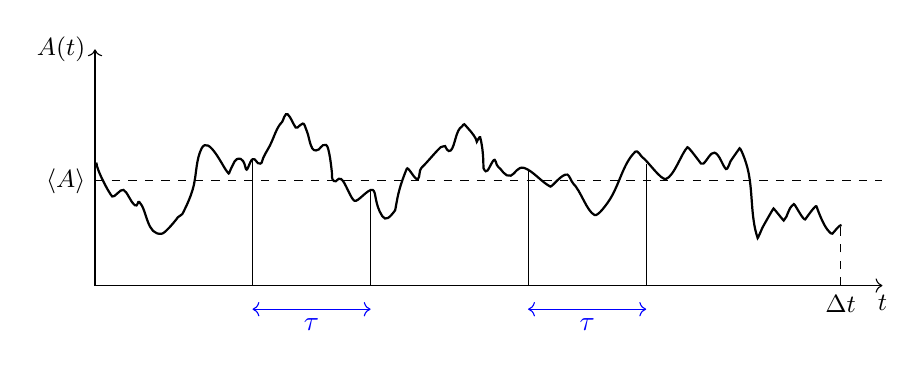
\begin{tikzpicture}
            \draw[->] (0,0)--(10,0)node[below]{\small\(t\)};
            \draw[->] (0,0)--(0,3)node[left]{\small\(A(t)\)};
            \begin{scope}[shift={(-0.25,0.5)}]
                \draw[scale=0.105,thick] (2.54,10.12) .. controls (2.54,9.31) and (4.08,6.38) .. (4.46,6.02) .. controls (4.7,5.78) and (5.45,6.99) .. (5.83,6.81) .. controls (6.29,6.59) and (6.64,5.39) .. (7.2,4.96) .. controls (7.55,4.68) and (7.53,5.56) .. (7.74,5.35) .. controls (8.69,4.44) and (8.61,1.21) .. (10.48,1.52) .. controls (10.84,1.57) and (12.04,2.98) .. (12.4,3.5) .. controls (12.53,3.68) and (12.85,3.7) .. (12.95,3.9) .. controls (13.51,4.99) and (14.04,6.15) .. (14.32,7.34) .. controls (14.66,8.81) and (14.61,10.54) .. (15.28,11.84) .. controls (16.14,13.52) and (17.89,9.45) .. (18.43,8.93) .. controls (18.69,8.68) and (18.44,8.66) .. (19,9.72) .. controls (19.28,10.25) and (19.29,10.4) .. (19.52,10.52) .. controls (19.71,10.61) and (20.27,10.83) .. (20.55,9.64) .. controls (20.76,8.49) and (21.03,10.32) .. (21.44,10.52) .. controls (21.87,10.72) and (21.87,9.86) .. (22.4,9.99) .. controls (22.46,10) and (22.52,10.06) .. (22.54,10.12) .. controls (22.75,10.93) and (23.11,11.36) .. (23.5,12.11) .. controls (24.05,13.17) and (24.32,14.36) .. (25,15.02) .. controls (25.13,15.14) and (25.37,16.26) .. (25.69,15.95) .. controls (26.1,15.55) and (26.3,14.86) .. (26.65,14.36) .. controls (26.86,14.04) and (27.5,15.32) .. (27.74,14.62) .. controls (27.96,13.98) and (28.13,13.67) .. (28.28,12.94) .. controls (28.56,11.8) and (28.73,11.58) .. (29.11,11.58) .. controls (29.68,11.58) and (29.71,12.44) .. (30.34,12.24) .. controls (30.72,12.12) and (31.02,9.04) .. (31.03,8.93) .. controls (31.06,8.57) and (30.97,8.03) .. (31.3,7.87) .. controls (31.65,7.7) and (31.7,8.34) .. (32.13,8.13) .. controls (32.62,7.89) and (33.3,5.71) .. (33.77,5.49) .. controls (34.17,5.29) and (35.41,6.99) .. (35.96,6.81) .. controls (36.42,6.66) and (36.15,5.13) .. (37.13,3.63) .. controls (37.55,3.02) and (37.98,3.41) .. (38.68,4.34) .. controls (38.96,5.66) and (38.96,6.59) .. (40.07,9.33) .. controls (40.21,9.85) and (41.12,7.83) .. (41.44,8.13) .. controls (41.71,8.39) and (41.55,9.17) .. (41.85,9.46) .. controls (42.57,10.16) and (43.5,11.32) .. (44.18,11.97) .. controls (44.19,11.98) and (44.69,12.14) .. (44.73,12.11) .. controls (44.75,12.08) and (45.06,11.23) .. (45.41,11.58) .. controls (45.94,12.09) and (46.01,14.12) .. (46.78,14.49) .. controls (46.86,14.53) and (46.95,14.88) .. (47.06,14.75) .. controls (47.65,14.09) and (48.15,13.56) .. (48.42,13.03) .. controls (48.45,12.98) and (48.56,12.64) .. (48.56,12.64) .. controls (48.56,12.64) and (48.92,13.36) .. (48.97,13.17) .. controls (49.28,11.97) and (49.36,10.65) .. (49.36,9.46) .. controls (49.78,8.53) and (49.92,9.33) .. (50.48,10.25) .. controls (50.91,10.91) and (50.82,9.76) .. (51.16,9.59) .. controls (51.49,9.43) and (51.96,8.3) .. (52.67,8.53) .. controls (53.19,8.7) and (53.47,9.73) .. (54.31,9.46) .. controls (55.31,9.14) and (56.49,7.68) .. (57.46,7.21) .. controls (57.63,7.13) and (58.91,8.86) .. (59.52,8.66) .. controls (59.76,8.59) and (60,7.8) .. (60.2,7.61) .. controls (61.16,6.68) and (61.86,4.22) .. (62.81,3.77) .. controls (63.2,3.58) and (64.21,5.01) .. (64.45,5.35) .. controls (65.85,7.38) and (66.17,9.93) .. (67.74,11.44) .. controls (67.99,11.69) and (68.43,10.87) .. (68.56,10.78) .. controls (69.2,10.37) and (70.83,7.94) .. (71.44,8.13) .. controls (72.41,8.45) and (73.35,11.31) .. (74.04,11.97) .. controls (74.15,12.08) and (75.6,10.07) .. (75.68,9.99) .. controls (75.75,9.93) and (75.88,9.94) .. (75.96,9.99) .. controls (76.32,10.22) and (76.87,11.46) .. (77.33,11.31) .. controls (77.94,11.11) and (78.26,9.75) .. (78.7,9.33) .. controls (78.86,9.16) and (79.18,10.13) .. (79.24,10.25) .. controls (79.33,10.43) and (80.34,11.84) .. (80.34,11.84) .. controls (80.34,11.84) and (80.45,11.76) .. (80.48,11.71) .. controls (80.77,11.14) and (81.09,10.26) .. (81.3,9.46) .. controls (81.99,6.76) and (81.63,3.61) .. (82.53,0.99) .. controls (82.55,0.93) and (83.01,2.01) .. (83.08,2.18) .. controls (83.14,2.32) and (84.39,4.53) .. (84.45,4.56) .. controls (84.49,4.58) and (85.66,3.08) .. (85.68,3.1) .. controls (86.27,3.67) and (86.1,4.5) .. (86.91,5.09) .. controls (87.02,5.16) and (88.02,3.11) .. (88.28,3.24) .. controls (88.3,3.24) and (89.56,5.1) .. (89.65,4.82) .. controls (89.94,3.98) and (90.57,2.35) .. (91.16,1.78) .. controls (91.28,1.67) and (91.45,1.4) .. (91.57,1.52) .. controls (91.89,1.82) and (92.36,2.57) .. (92.67,2.57) ;
            \end{scope}
            \draw[dashed] (0,1.33)node[left]{\small\(\eval{A}\)}--(10,1.33);
            \draw[dashed] (9.47,0)node[below]{\small\(\Delta t\)}--(9.47,0.77);
            \draw (2,0)--(2,1.6);
            \draw (3.5,0)--(3.5,1.2);
            \draw[<->,blue] (2,-0.3)--node[below]{\(\tau\)}(3.5,-0.3);
            \draw (5.5,0)--(5.5,1.45);
            \draw (7,0)--(7,1.55);
            \draw[<->,blue] (5.5,-0.3)--node[below]{\(\tau\)}(7,-0.3);
        \end{tikzpicture}
        \caption{Constructing the autocorrelation function of a quantity.}
    \end{figure}

    Hence, one can extract the transport coefficients from an MD simulation at equilibrium using Green--Kubo relations from the following scheme:
    \begin{enumerate}[topsep=0pt]
        \item Run a simulation at equilibrium.
        \item Compute relevant microscopic quantity. For example, if we are interested in the diffusion coefficient, then we can calculate the particle's velocity.
        \item Calculate the autocorrelation function.
        \item Integrate to get the transport coefficient.
    \end{enumerate}

    One can generalise the autocorrelation function to define the \textit{cross-correlation function}\footnote{More formally, it can also be defined using a phase-space average as an ergodic integral
    \begin{equation}
        C_{AB}(\tau)\coloneqq\int\dd[3N]{\vb{r}^N}\dd[3N]{\vb{p}^N}A(\vb{r}^N,\vb{p}^N)B(\tau\mid\vb{r}^N,\vb{p}^N)\rho(\vb{r}^N,\vb{p}^N)\,.
    \end{equation}}
    \begin{equation}
        C_{\text{AB}}(\tau)\coloneqq\frac{\eval{A(t)B(t+\tau)}}{\eval{A}\eval{B}}\,.
    \end{equation}
    Where the normalisation factor may be there or not. This will be useful when studying coupled processes, like energy transfer or reaction rates. The loss of correlation with time is usually an exponential decay, and the decorrelation time can be estimated from a time integral over the correlation function
    \begin{equation}
        \tau_{AB}=\frac{1}{C_{AB}(0)}\int_{0}^{\infty}\dd{\tau}C_{AB}(\tau)\,.
    \end{equation}
    One may check that the correlation function has the time translation invariance and time inversion symmetry
    \begin{align}
        \eval{A(t+\tau)B(t)}&=\eval{A(t'+\tau)B(t')}\\
        \eval{A(\tau)A(0)}&=\eval{A(0)A(-\tau)}\,.
    \end{align}
    \subsubsection{Fluctuation-Dissipation Theorem}
    In fact, the use of time correlation function at equilibrium in obtaining off-equilibrium properties like transport coefficient is a very deep and profound result related to the fluctuation-dissipation theorem.
    
    An informal statement of this theorem is Onsager's \textit{regression hypothesis}: the relaxation of a system after some macroscopic perturbation is governed by the same laws as the regressions of spontaneous microscopic fluctuations in an equilibrium system. A system's fluctuation at equilibrium is indistinguishable from its approach from off-equilibrium to equilibrium, provided that it is not too far away from equilibrium. The fluctuation-dissipation theorem formalises this hypothesis.

    \begin{thm}[Fluctuation-dissipation theorem]
        Consider a system that has been prepared in a state sampled from some non-equilibrium distribution \(F(\vb{r}^N,\vb{p}^N)\) by the means of a small perturbation \(\Delta H\). Write the average of the observable \(A\) in the perturbed state as
        \begin{equation}
            \overline{A}(t)=\int\dd[3N]{\vb{r}^N}\dd[3N]{\vb{p}^N}A(t\mid\vb{r}^N,\vb{p}^N)F(\vb{r}^N,\vb{p}^N)\,.
        \end{equation}
        If the initial state is not too far from equilibrium, the time evolution follows
        \begin{equation}
            \frac{\overline{A}(t)}{\overline{A}(0)}=\frac{C_{AA}(t)}{C_{AA}(0)}\,.
        \end{equation}
    \end{thm}

    Hence, instead of measuring how a system responds to an external force, we can directly measure how it fluctuates at equilibrium.

    \subsection{Force Fields}
    A force field is the classical parameterisation of the adiabatic potential energy surface \(V(\vb{r}^N)\). It can be separated into bonded and non-bonded potentials to include both bonded and non-bonded interactions.

    Bonded potentials capture covalent, intramolecular interactions. They are usually partitioned onto \(n\)-body terms up to \(n=4\).
    \begin{figure}[ht!]
        \centering
        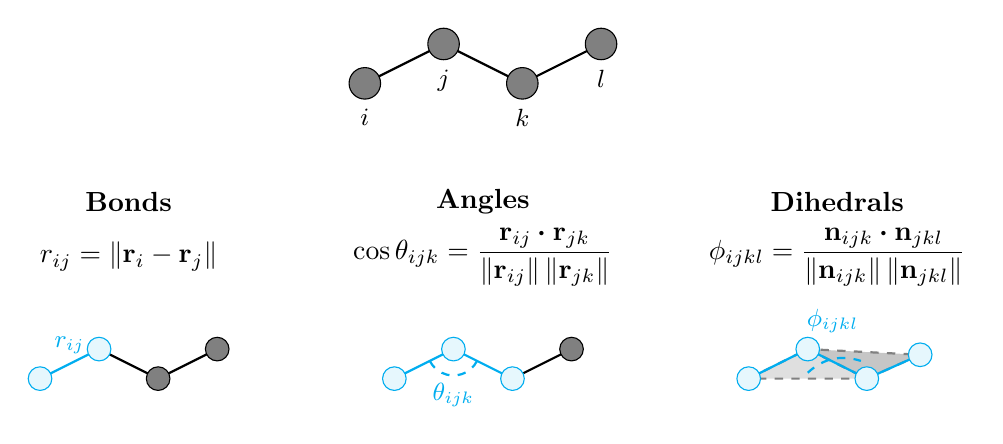
\begin{tikzpicture}
            \draw[thick] (0,0)node[below=0.2cm]{\small\(i\)}--(1,0.5)node[below=0.2cm]{\small\(j\)}--(2,0)node[below=0.2cm]{\small\(k\)}--(3,0.5)node[below=0.2cm]{\small\(l\)};
            \draw[fill=gray] (0,0) circle(0.2);
            \draw[fill=gray] (1,0.5) circle(0.2);
            \draw[fill=gray] (2,0) circle(0.2);
            \draw[fill=gray] (3,0.5) circle(0.2);
            \begin{scope}[shift={(-3,-1.5)}]
                \node at (0,0){\textbf{Bonds}};
                \node at (0,-0.7){\(\displaystyle r_{ij}=\norm{\vb{r}_i-\vb{r}_j}\)};
                \begin{scope}[scale=0.75,shift={(-1.5,-3)}]
                    \draw[thick,cyan] (0,0)--node[above]{\small\(r_{ij}\)}(1,0.5);
                    \draw[thick] (1,0.5)--(2,0)--(3,0.5);
                    \draw[cyan,fill=cyan!10] (0,0) circle(0.2);
                    \draw[cyan,fill=cyan!10] (1,0.5) circle(0.2);
                    \draw[fill=gray] (2,0) circle(0.2);
                    \draw[fill=gray] (3,0.5) circle(0.2);
                \end{scope}
            \end{scope}
            \begin{scope}[shift={(1.5,-1.5)}]
                \node at (0,0){\textbf{Angles}};
                \node at (0,-0.7){\(\displaystyle\cos\theta_{ijk}=\frac{\vb{r}_{ij}\vdot\vb{r}_{jk}}{\norm{\vb{r}_{ij}}\norm{\vb{r}_{jk}}}\)};
                \begin{scope}[scale=0.75,shift={(-1.5,-3)}]
                    \draw[thick,cyan] (0,0)--(1,0.5)node[below=0.3cm]{\small\(\theta_{ijk}\)}--(2,0);
                    \draw[dashed,cyan,thick] (1.4,0.3) arc(-26.56:-153.43:0.447);
                    \draw[thick] (2,0)--(3,0.5);
                    \draw[cyan,fill=cyan!10] (0,0) circle(0.2);
                    \draw[cyan,fill=cyan!10] (1,0.5) circle(0.2);
                    \draw[cyan,fill=cyan!10] (2,0) circle(0.2);
                    \draw[fill=gray] (3,0.5) circle(0.2);
                \end{scope}
            \end{scope}
            \begin{scope}[shift={(6,-1.5)}]
                \node at (0,0){\textbf{Dihedrals}};
                \node at (0,-0.7){\(\displaystyle\phi_{ijkl}=\frac{\vb{n}_{ijk}\vdot\vb{n}_{jkl}}{\norm{\vb{n}_{ijk}}\norm{\vb{n}_{jkl}}}\)};
                \begin{scope}[scale=0.75,shift={(-1.5,-3)}]
                    \draw[thick,dashed,gray,fill=gray!25] (0,0)--(1,0.5)--(2,0)--(0,0);
                    \draw[thick,dashed,gray,fill=gray!45] (1,0.5)--(2,0)--(3,0.5,0.25)--(1,0.5);
                    \draw[thick,cyan] (0,0)--(1,0.5)--(2,0)--(3,0.5,0.25);
                    \draw[dashed, thick, cyan] (1,0.1) to[bend left]node[above=0.2cm]{\small\(\phi_{ijkl}\)} (1.9,0.3);
                    \draw[cyan,fill=cyan!10] (0,0) circle(0.2);
                    \draw[cyan,fill=cyan!10] (1,0.5) circle(0.2);
                    \draw[cyan,fill=cyan!10] (2,0) circle(0.2);
                    \draw[cyan,fill=cyan!10] (3,0.5,0.25) circle(0.2);
                \end{scope}
            \end{scope}
        \end{tikzpicture}
    \end{figure}

    Some commonly used bonded potentials are
    \begin{itemize}[topsep=0pt]
        \item Harmonic bond.
        \begin{equation}
            u(r_{ij})=\frac{1}{2}k_r(r_{ij}-r_0)^2\,.
        \end{equation}
        \item Harmonic angle.
        \begin{equation}
            u(\theta_{ijk})=\frac{1}{2}k_\theta(\theta_{ijk}-\theta_0)^2\,.
        \end{equation}
        \item Proper dihedral. It simulates the conditions where several dihedral angles are likely, and it has many probable forms. The Ryckaert--Bellemans form is
        \begin{equation}
            u_{rb}(\phi_{ijkl})=\sum_{n=0}^{5}c_n\cos^n(\phi_{ijkl})\,.
        \end{equation}
        It is a \(2\pi\)-periodic function with several minima and maxima.
        \item Improper dihedral. It is used to capture the rigidity of certain systems like planar \(\mathrm{BF_3}\), where only one specific dihedral angle is probable.
        \begin{equation}
            u_{id}(\phi_{ijkl})=\frac{1}{2}k_\phi(\phi_{ijkl}-\phi_0)^2\,.
        \end{equation}
    \end{itemize}

    Non-bonded potentials capture van der Waals, electrostatic and polarisation interactions at both intermolecular and intramolecular levels. These interactions are often approximated using only pairwise terms.
    \begin{figure}[ht!]
        \centering
        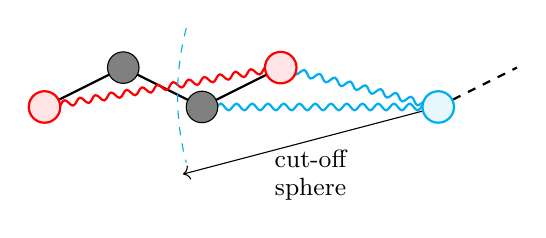
\begin{tikzpicture}[decoration = {snake,amplitude=1.2pt,segment length=2mm}]
            \draw[thick] (0,0)--(1,0.5)--(2,0)--(3,0.5);
            \draw[decorate,thick,red] (0,0)--(3,0.5);
            \draw[decorate,thick,cyan] (5,0)--(3,0.5);
            \draw[decorate,thick,cyan] (5,0)--(2,0);
            \draw[thick,red,fill=red!10] (0,0) circle(0.2);
            \draw[fill=gray] (1,0.5) circle(0.2);
            \draw[fill=gray] (2,0) circle(0.2);
            \draw[thick,red,fill=red!10] (3,0.5) circle(0.2);
            \draw[thick,dashed] (5,0)--(6,0.5);
            \draw[->,align=center] (5,0)--node[below]{\small cut-off \\[-2pt] \small sphere}+(194.74:3.353);
            \draw[thick,cyan,fill=cyan!10] (5,0) circle(0.2);
            \draw[dashed,cyan] (1.8,1) arc (165.26:194.74:3.353);
        \end{tikzpicture}
        \caption{Both intermolecular and intramolecular non-bonded forces should be considered. However, 1-2 and 1-3 interactions are often excluded.}
    \end{figure}

    Common non-bonded potentials include:
    \begin{itemize}[topsep=0pt]
        \item Lennard-Jones potential
        \begin{equation}
            u_{\text{LJ}}(r_{ij})=4\epsilon_{ij}f_{\text{LJ}}(r_{ij})\left(\frac{A_{ij}}{r_{ij}^{12}}-\frac{B_{ij}}{r_{ij}^6}\right)\,,
        \end{equation}
        where \(f_{ij}(r_{ij})\) is a cut-off function such that \(f_{\text{LJ}}(r_{ij})=0\) for \(r_{ij}\) above the cut-off radius and one otherwise. The most common way obtaining these coefficients is the Lorentz-Berthelot rules
        \begin{align}
            \epsilon_{ij}&=\sqrt{\epsilon_i\epsilon_j} & \sigma_{ij}&=\frac{\sigma_i+\sigma_j}{2} \\
            A_{ij}&=4\epsilon_{ij}\sigma_{ij}^{12} & B_{ij}&=4\epsilon_{ij}\sigma_{ij}^6\,.
        \end{align}
        \item Coulomb potential
        \begin{equation}
            u_{ij}=f_c(r_{ij})\frac{1}{4\pi\epsilon_0}\frac{q_iq_j}{r_{ij}}\,.
        \end{equation}
    \end{itemize}

    \subsection{Errors in Simulations}
    Broadly speaking, the errors in an MD simulation can be classified into two categories. First, there are systematic errors that are inherent to the system. It is related to the model and method one uses to describe a given system (e.g. force field, quantum mechanical effect), and it is harder to gain control over. There are also \textit{statistical errors} that can arise in either time domain due to finite sampling, or in spatial domain due to finite size effects. We will focus on statistical errors.

    \subsubsection{Block Average Method}
    If we have a trajectory of length \(\tau\), the average of a dynamical observable \(A\) over this trajectory can be calculated as
    \begin{equation}
        A_\tau=\frac{1}{\tau}\int_0^\tau \dd{t}A(t)\,.
    \end{equation}
    In the limit of infinite simulation time, the estimated average should converge to the true ensemble average
    \begin{equation}
        \lim_{\tau\to\infty}\eval{A_\tau}=\eval{A}\,.
    \end{equation}
    But we can only simulate the system for a finite amount of time. Then how do we calculate the error of our estimate \(A_\tau\)?

    \begin{figure}[ht!]
        \centering
        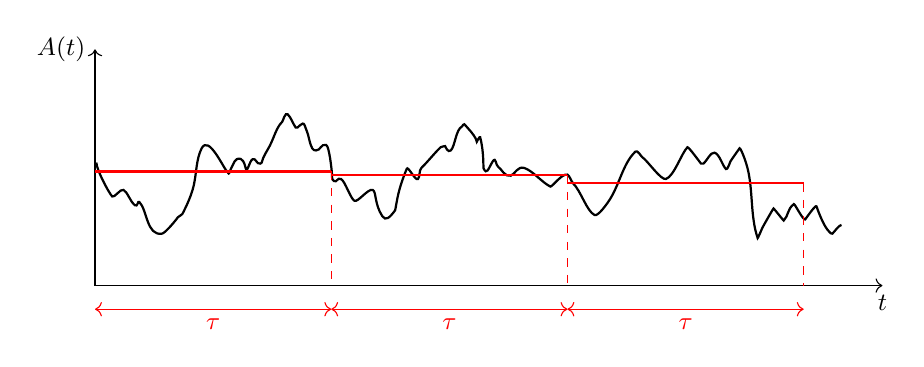
\begin{tikzpicture}
            \draw[->] (0,0)--(10,0)node[below]{\small\(t\)};
            \draw[->] (0,0)--(0,3)node[left]{\small\(A(t)\)};
            \begin{scope}[shift={(-0.25,0.5)}]
                \draw[scale=0.105,thick] (2.54,10.12) .. controls (2.54,9.31) and (4.08,6.38) .. (4.46,6.02) .. controls (4.7,5.78) and (5.45,6.99) .. (5.83,6.81) .. controls (6.29,6.59) and (6.64,5.39) .. (7.2,4.96) .. controls (7.55,4.68) and (7.53,5.56) .. (7.74,5.35) .. controls (8.69,4.44) and (8.61,1.21) .. (10.48,1.52) .. controls (10.84,1.57) and (12.04,2.98) .. (12.4,3.5) .. controls (12.53,3.68) and (12.85,3.7) .. (12.95,3.9) .. controls (13.51,4.99) and (14.04,6.15) .. (14.32,7.34) .. controls (14.66,8.81) and (14.61,10.54) .. (15.28,11.84) .. controls (16.14,13.52) and (17.89,9.45) .. (18.43,8.93) .. controls (18.69,8.68) and (18.44,8.66) .. (19,9.72) .. controls (19.28,10.25) and (19.29,10.4) .. (19.52,10.52) .. controls (19.71,10.61) and (20.27,10.83) .. (20.55,9.64) .. controls (20.76,8.49) and (21.03,10.32) .. (21.44,10.52) .. controls (21.87,10.72) and (21.87,9.86) .. (22.4,9.99) .. controls (22.46,10) and (22.52,10.06) .. (22.54,10.12) .. controls (22.75,10.93) and (23.11,11.36) .. (23.5,12.11) .. controls (24.05,13.17) and (24.32,14.36) .. (25,15.02) .. controls (25.13,15.14) and (25.37,16.26) .. (25.69,15.95) .. controls (26.1,15.55) and (26.3,14.86) .. (26.65,14.36) .. controls (26.86,14.04) and (27.5,15.32) .. (27.74,14.62) .. controls (27.96,13.98) and (28.13,13.67) .. (28.28,12.94) .. controls (28.56,11.8) and (28.73,11.58) .. (29.11,11.58) .. controls (29.68,11.58) and (29.71,12.44) .. (30.34,12.24) .. controls (30.72,12.12) and (31.02,9.04) .. (31.03,8.93) .. controls (31.06,8.57) and (30.97,8.03) .. (31.3,7.87) .. controls (31.65,7.7) and (31.7,8.34) .. (32.13,8.13) .. controls (32.62,7.89) and (33.3,5.71) .. (33.77,5.49) .. controls (34.17,5.29) and (35.41,6.99) .. (35.96,6.81) .. controls (36.42,6.66) and (36.15,5.13) .. (37.13,3.63) .. controls (37.55,3.02) and (37.98,3.41) .. (38.68,4.34) .. controls (38.96,5.66) and (38.96,6.59) .. (40.07,9.33) .. controls (40.21,9.85) and (41.12,7.83) .. (41.44,8.13) .. controls (41.71,8.39) and (41.55,9.17) .. (41.85,9.46) .. controls (42.57,10.16) and (43.5,11.32) .. (44.18,11.97) .. controls (44.19,11.98) and (44.69,12.14) .. (44.73,12.11) .. controls (44.75,12.08) and (45.06,11.23) .. (45.41,11.58) .. controls (45.94,12.09) and (46.01,14.12) .. (46.78,14.49) .. controls (46.86,14.53) and (46.95,14.88) .. (47.06,14.75) .. controls (47.65,14.09) and (48.15,13.56) .. (48.42,13.03) .. controls (48.45,12.98) and (48.56,12.64) .. (48.56,12.64) .. controls (48.56,12.64) and (48.92,13.36) .. (48.97,13.17) .. controls (49.28,11.97) and (49.36,10.65) .. (49.36,9.46) .. controls (49.78,8.53) and (49.92,9.33) .. (50.48,10.25) .. controls (50.91,10.91) and (50.82,9.76) .. (51.16,9.59) .. controls (51.49,9.43) and (51.96,8.3) .. (52.67,8.53) .. controls (53.19,8.7) and (53.47,9.73) .. (54.31,9.46) .. controls (55.31,9.14) and (56.49,7.68) .. (57.46,7.21) .. controls (57.63,7.13) and (58.91,8.86) .. (59.52,8.66) .. controls (59.76,8.59) and (60,7.8) .. (60.2,7.61) .. controls (61.16,6.68) and (61.86,4.22) .. (62.81,3.77) .. controls (63.2,3.58) and (64.21,5.01) .. (64.45,5.35) .. controls (65.85,7.38) and (66.17,9.93) .. (67.74,11.44) .. controls (67.99,11.69) and (68.43,10.87) .. (68.56,10.78) .. controls (69.2,10.37) and (70.83,7.94) .. (71.44,8.13) .. controls (72.41,8.45) and (73.35,11.31) .. (74.04,11.97) .. controls (74.15,12.08) and (75.6,10.07) .. (75.68,9.99) .. controls (75.75,9.93) and (75.88,9.94) .. (75.96,9.99) .. controls (76.32,10.22) and (76.87,11.46) .. (77.33,11.31) .. controls (77.94,11.11) and (78.26,9.75) .. (78.7,9.33) .. controls (78.86,9.16) and (79.18,10.13) .. (79.24,10.25) .. controls (79.33,10.43) and (80.34,11.84) .. (80.34,11.84) .. controls (80.34,11.84) and (80.45,11.76) .. (80.48,11.71) .. controls (80.77,11.14) and (81.09,10.26) .. (81.3,9.46) .. controls (81.99,6.76) and (81.63,3.61) .. (82.53,0.99) .. controls (82.55,0.93) and (83.01,2.01) .. (83.08,2.18) .. controls (83.14,2.32) and (84.39,4.53) .. (84.45,4.56) .. controls (84.49,4.58) and (85.66,3.08) .. (85.68,3.1) .. controls (86.27,3.67) and (86.1,4.5) .. (86.91,5.09) .. controls (87.02,5.16) and (88.02,3.11) .. (88.28,3.24) .. controls (88.3,3.24) and (89.56,5.1) .. (89.65,4.82) .. controls (89.94,3.98) and (90.57,2.35) .. (91.16,1.78) .. controls (91.28,1.67) and (91.45,1.4) .. (91.57,1.52) .. controls (91.89,1.82) and (92.36,2.57) .. (92.67,2.57) ;
            \end{scope}
            \draw[thick,red](0,1.45)--(3,1.45);
            \draw[thick,red](3,1.4)--(6,1.4);
            \draw[thick,red](6,1.3)--(9,1.3);
            \draw[dashed,red](3,1.45)--(3,0);
            \draw[dashed,red](6,1.4)--(6,0);
            \draw[dashed,red](9,1.3)--(9,0);
            \draw[<->,red] (0,-0.3)--node[below]{\small\(\tau\)}(3,-0.3);
            \draw[<->,red] (3,-0.3)--node[below]{\small\(\tau\)}(6,-0.3);
            \draw[<->,red] (6,-0.3)--node[below]{\small\(\tau\)}(9,-0.3);
        \end{tikzpicture}
        \caption{Estimating the statistical error using the block average method.}
    \end{figure}

    To estimate the error, we can consider finite blocks that partition the trajectory onto smaller chunks, and then evaluate the average of \(A\) over each block. For a given choice of \(\tau\), the variance of \(A_\tau\) is given by
    \begin{equation}
        \sigma^2(A_\tau)=\sum_{b=1}^{n_b}\frac{(A_{\tau,b}-A_{\Delta t})^2}{n_b}\,.
    \end{equation}
    Clearly, the estimated variance will be strongly dependent on the choice of \(\tau\). If we use \(\tau=\Delta t\), then we get \(\sigma^2(A_\tau)=0\) and this clearly underestimates the error. If we choose too small a \(\tau\), then we would overestimate the error. How do we choose the appropriate block size?

    \begin{figure}
        \centering
        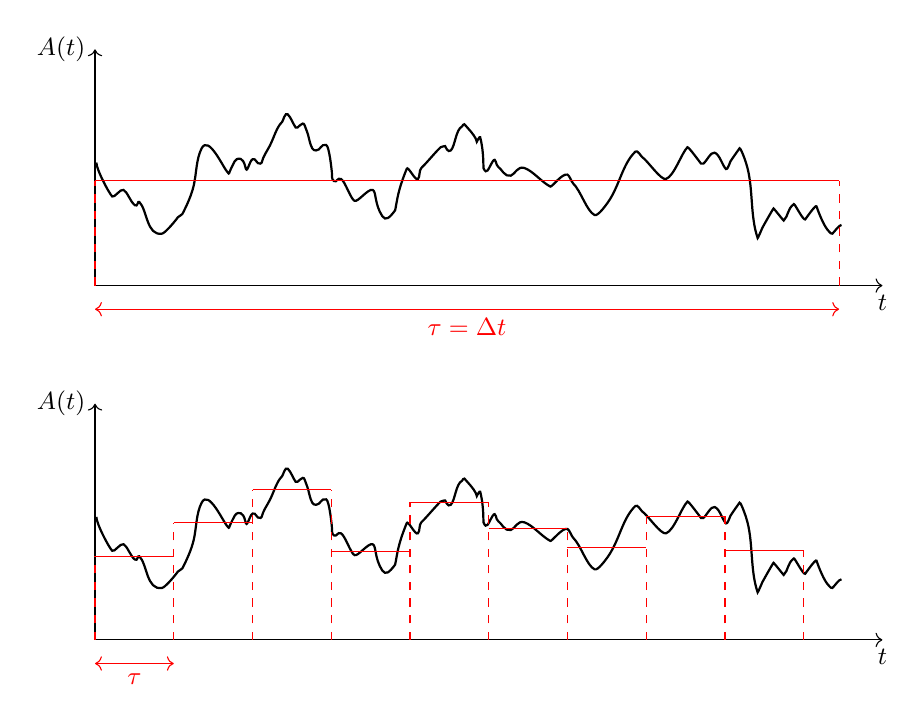
\begin{tikzpicture}
            \draw[->] (0,0)--(10,0)node[below]{\small\(t\)};
            \draw[->] (0,0)--(0,3)node[left]{\small\(A(t)\)};
            \begin{scope}[shift={(-0.25,0.5)}]
                \draw[scale=0.105,thick] (2.54,10.12) .. controls (2.54,9.31) and (4.08,6.38) .. (4.46,6.02) .. controls (4.7,5.78) and (5.45,6.99) .. (5.83,6.81) .. controls (6.29,6.59) and (6.64,5.39) .. (7.2,4.96) .. controls (7.55,4.68) and (7.53,5.56) .. (7.74,5.35) .. controls (8.69,4.44) and (8.61,1.21) .. (10.48,1.52) .. controls (10.84,1.57) and (12.04,2.98) .. (12.4,3.5) .. controls (12.53,3.68) and (12.85,3.7) .. (12.95,3.9) .. controls (13.51,4.99) and (14.04,6.15) .. (14.32,7.34) .. controls (14.66,8.81) and (14.61,10.54) .. (15.28,11.84) .. controls (16.14,13.52) and (17.89,9.45) .. (18.43,8.93) .. controls (18.69,8.68) and (18.44,8.66) .. (19,9.72) .. controls (19.28,10.25) and (19.29,10.4) .. (19.52,10.52) .. controls (19.71,10.61) and (20.27,10.83) .. (20.55,9.64) .. controls (20.76,8.49) and (21.03,10.32) .. (21.44,10.52) .. controls (21.87,10.72) and (21.87,9.86) .. (22.4,9.99) .. controls (22.46,10) and (22.52,10.06) .. (22.54,10.12) .. controls (22.75,10.93) and (23.11,11.36) .. (23.5,12.11) .. controls (24.05,13.17) and (24.32,14.36) .. (25,15.02) .. controls (25.13,15.14) and (25.37,16.26) .. (25.69,15.95) .. controls (26.1,15.55) and (26.3,14.86) .. (26.65,14.36) .. controls (26.86,14.04) and (27.5,15.32) .. (27.74,14.62) .. controls (27.96,13.98) and (28.13,13.67) .. (28.28,12.94) .. controls (28.56,11.8) and (28.73,11.58) .. (29.11,11.58) .. controls (29.68,11.58) and (29.71,12.44) .. (30.34,12.24) .. controls (30.72,12.12) and (31.02,9.04) .. (31.03,8.93) .. controls (31.06,8.57) and (30.97,8.03) .. (31.3,7.87) .. controls (31.65,7.7) and (31.7,8.34) .. (32.13,8.13) .. controls (32.62,7.89) and (33.3,5.71) .. (33.77,5.49) .. controls (34.17,5.29) and (35.41,6.99) .. (35.96,6.81) .. controls (36.42,6.66) and (36.15,5.13) .. (37.13,3.63) .. controls (37.55,3.02) and (37.98,3.41) .. (38.68,4.34) .. controls (38.96,5.66) and (38.96,6.59) .. (40.07,9.33) .. controls (40.21,9.85) and (41.12,7.83) .. (41.44,8.13) .. controls (41.71,8.39) and (41.55,9.17) .. (41.85,9.46) .. controls (42.57,10.16) and (43.5,11.32) .. (44.18,11.97) .. controls (44.19,11.98) and (44.69,12.14) .. (44.73,12.11) .. controls (44.75,12.08) and (45.06,11.23) .. (45.41,11.58) .. controls (45.94,12.09) and (46.01,14.12) .. (46.78,14.49) .. controls (46.86,14.53) and (46.95,14.88) .. (47.06,14.75) .. controls (47.65,14.09) and (48.15,13.56) .. (48.42,13.03) .. controls (48.45,12.98) and (48.56,12.64) .. (48.56,12.64) .. controls (48.56,12.64) and (48.92,13.36) .. (48.97,13.17) .. controls (49.28,11.97) and (49.36,10.65) .. (49.36,9.46) .. controls (49.78,8.53) and (49.92,9.33) .. (50.48,10.25) .. controls (50.91,10.91) and (50.82,9.76) .. (51.16,9.59) .. controls (51.49,9.43) and (51.96,8.3) .. (52.67,8.53) .. controls (53.19,8.7) and (53.47,9.73) .. (54.31,9.46) .. controls (55.31,9.14) and (56.49,7.68) .. (57.46,7.21) .. controls (57.63,7.13) and (58.91,8.86) .. (59.52,8.66) .. controls (59.76,8.59) and (60,7.8) .. (60.2,7.61) .. controls (61.16,6.68) and (61.86,4.22) .. (62.81,3.77) .. controls (63.2,3.58) and (64.21,5.01) .. (64.45,5.35) .. controls (65.85,7.38) and (66.17,9.93) .. (67.74,11.44) .. controls (67.99,11.69) and (68.43,10.87) .. (68.56,10.78) .. controls (69.2,10.37) and (70.83,7.94) .. (71.44,8.13) .. controls (72.41,8.45) and (73.35,11.31) .. (74.04,11.97) .. controls (74.15,12.08) and (75.6,10.07) .. (75.68,9.99) .. controls (75.75,9.93) and (75.88,9.94) .. (75.96,9.99) .. controls (76.32,10.22) and (76.87,11.46) .. (77.33,11.31) .. controls (77.94,11.11) and (78.26,9.75) .. (78.7,9.33) .. controls (78.86,9.16) and (79.18,10.13) .. (79.24,10.25) .. controls (79.33,10.43) and (80.34,11.84) .. (80.34,11.84) .. controls (80.34,11.84) and (80.45,11.76) .. (80.48,11.71) .. controls (80.77,11.14) and (81.09,10.26) .. (81.3,9.46) .. controls (81.99,6.76) and (81.63,3.61) .. (82.53,0.99) .. controls (82.55,0.93) and (83.01,2.01) .. (83.08,2.18) .. controls (83.14,2.32) and (84.39,4.53) .. (84.45,4.56) .. controls (84.49,4.58) and (85.66,3.08) .. (85.68,3.1) .. controls (86.27,3.67) and (86.1,4.5) .. (86.91,5.09) .. controls (87.02,5.16) and (88.02,3.11) .. (88.28,3.24) .. controls (88.3,3.24) and (89.56,5.1) .. (89.65,4.82) .. controls (89.94,3.98) and (90.57,2.35) .. (91.16,1.78) .. controls (91.28,1.67) and (91.45,1.4) .. (91.57,1.52) .. controls (91.89,1.82) and (92.36,2.57) .. (92.67,2.57) ;
            \end{scope}
            \draw[red] (0,1.33)--(9.45,1.33);
            \draw[red,dashed](0,0)--(0,1.33);
            \draw[red,dashed](9.45,0)--(9.45,1.33);
            \draw[<->,red](0,-0.3)--node[below]{\small\(\tau=\Delta t\)}(9.45,-0.3);
            \begin{scope}[shift={(0,-4.5)}]
                \draw[->] (0,0)--(10,0)node[below]{\small\(t\)};
                \draw[->] (0,0)--(0,3)node[left]{\small\(A(t)\)};
                \begin{scope}[shift={(-0.25,0.5)}]
                    \draw[scale=0.105,thick] (2.54,10.12) .. controls (2.54,9.31) and (4.08,6.38) .. (4.46,6.02) .. controls (4.7,5.78) and (5.45,6.99) .. (5.83,6.81) .. controls (6.29,6.59) and (6.64,5.39) .. (7.2,4.96) .. controls (7.55,4.68) and (7.53,5.56) .. (7.74,5.35) .. controls (8.69,4.44) and (8.61,1.21) .. (10.48,1.52) .. controls (10.84,1.57) and (12.04,2.98) .. (12.4,3.5) .. controls (12.53,3.68) and (12.85,3.7) .. (12.95,3.9) .. controls (13.51,4.99) and (14.04,6.15) .. (14.32,7.34) .. controls (14.66,8.81) and (14.61,10.54) .. (15.28,11.84) .. controls (16.14,13.52) and (17.89,9.45) .. (18.43,8.93) .. controls (18.69,8.68) and (18.44,8.66) .. (19,9.72) .. controls (19.28,10.25) and (19.29,10.4) .. (19.52,10.52) .. controls (19.71,10.61) and (20.27,10.83) .. (20.55,9.64) .. controls (20.76,8.49) and (21.03,10.32) .. (21.44,10.52) .. controls (21.87,10.72) and (21.87,9.86) .. (22.4,9.99) .. controls (22.46,10) and (22.52,10.06) .. (22.54,10.12) .. controls (22.75,10.93) and (23.11,11.36) .. (23.5,12.11) .. controls (24.05,13.17) and (24.32,14.36) .. (25,15.02) .. controls (25.13,15.14) and (25.37,16.26) .. (25.69,15.95) .. controls (26.1,15.55) and (26.3,14.86) .. (26.65,14.36) .. controls (26.86,14.04) and (27.5,15.32) .. (27.74,14.62) .. controls (27.96,13.98) and (28.13,13.67) .. (28.28,12.94) .. controls (28.56,11.8) and (28.73,11.58) .. (29.11,11.58) .. controls (29.68,11.58) and (29.71,12.44) .. (30.34,12.24) .. controls (30.72,12.12) and (31.02,9.04) .. (31.03,8.93) .. controls (31.06,8.57) and (30.97,8.03) .. (31.3,7.87) .. controls (31.65,7.7) and (31.7,8.34) .. (32.13,8.13) .. controls (32.62,7.89) and (33.3,5.71) .. (33.77,5.49) .. controls (34.17,5.29) and (35.41,6.99) .. (35.96,6.81) .. controls (36.42,6.66) and (36.15,5.13) .. (37.13,3.63) .. controls (37.55,3.02) and (37.98,3.41) .. (38.68,4.34) .. controls (38.96,5.66) and (38.96,6.59) .. (40.07,9.33) .. controls (40.21,9.85) and (41.12,7.83) .. (41.44,8.13) .. controls (41.71,8.39) and (41.55,9.17) .. (41.85,9.46) .. controls (42.57,10.16) and (43.5,11.32) .. (44.18,11.97) .. controls (44.19,11.98) and (44.69,12.14) .. (44.73,12.11) .. controls (44.75,12.08) and (45.06,11.23) .. (45.41,11.58) .. controls (45.94,12.09) and (46.01,14.12) .. (46.78,14.49) .. controls (46.86,14.53) and (46.95,14.88) .. (47.06,14.75) .. controls (47.65,14.09) and (48.15,13.56) .. (48.42,13.03) .. controls (48.45,12.98) and (48.56,12.64) .. (48.56,12.64) .. controls (48.56,12.64) and (48.92,13.36) .. (48.97,13.17) .. controls (49.28,11.97) and (49.36,10.65) .. (49.36,9.46) .. controls (49.78,8.53) and (49.92,9.33) .. (50.48,10.25) .. controls (50.91,10.91) and (50.82,9.76) .. (51.16,9.59) .. controls (51.49,9.43) and (51.96,8.3) .. (52.67,8.53) .. controls (53.19,8.7) and (53.47,9.73) .. (54.31,9.46) .. controls (55.31,9.14) and (56.49,7.68) .. (57.46,7.21) .. controls (57.63,7.13) and (58.91,8.86) .. (59.52,8.66) .. controls (59.76,8.59) and (60,7.8) .. (60.2,7.61) .. controls (61.16,6.68) and (61.86,4.22) .. (62.81,3.77) .. controls (63.2,3.58) and (64.21,5.01) .. (64.45,5.35) .. controls (65.85,7.38) and (66.17,9.93) .. (67.74,11.44) .. controls (67.99,11.69) and (68.43,10.87) .. (68.56,10.78) .. controls (69.2,10.37) and (70.83,7.94) .. (71.44,8.13) .. controls (72.41,8.45) and (73.35,11.31) .. (74.04,11.97) .. controls (74.15,12.08) and (75.6,10.07) .. (75.68,9.99) .. controls (75.75,9.93) and (75.88,9.94) .. (75.96,9.99) .. controls (76.32,10.22) and (76.87,11.46) .. (77.33,11.31) .. controls (77.94,11.11) and (78.26,9.75) .. (78.7,9.33) .. controls (78.86,9.16) and (79.18,10.13) .. (79.24,10.25) .. controls (79.33,10.43) and (80.34,11.84) .. (80.34,11.84) .. controls (80.34,11.84) and (80.45,11.76) .. (80.48,11.71) .. controls (80.77,11.14) and (81.09,10.26) .. (81.3,9.46) .. controls (81.99,6.76) and (81.63,3.61) .. (82.53,0.99) .. controls (82.55,0.93) and (83.01,2.01) .. (83.08,2.18) .. controls (83.14,2.32) and (84.39,4.53) .. (84.45,4.56) .. controls (84.49,4.58) and (85.66,3.08) .. (85.68,3.1) .. controls (86.27,3.67) and (86.1,4.5) .. (86.91,5.09) .. controls (87.02,5.16) and (88.02,3.11) .. (88.28,3.24) .. controls (88.3,3.24) and (89.56,5.1) .. (89.65,4.82) .. controls (89.94,3.98) and (90.57,2.35) .. (91.16,1.78) .. controls (91.28,1.67) and (91.45,1.4) .. (91.57,1.52) .. controls (91.89,1.82) and (92.36,2.57) .. (92.67,2.57) ;
                \end{scope}
                \draw[red] (0,1.06)--(1,1.06);
                \draw[red] (1,1.49)--(2,1.49);
                \draw[red] (2,1.91)--(3,1.91);
                \draw[red] (3,1.12)--(4,1.12);
                \draw[red] (4,1.75)--(5,1.75);
                \draw[red] (5,1.42)--(6,1.42);
                \draw[red] (6,1.17)--(7,1.17);
                \draw[red] (7,1.57)--(8,1.57);
                \draw[red] (8,1.14)--(9,1.14);
                \draw[dashed,red] (0,0)--(0,1.06);
                \draw[dashed,red] (1,0)--(1,1.49);
                \draw[dashed,red] (2,0)--(2,1.91);
                \draw[dashed,red] (3,0)--(3,1.91);
                \draw[dashed,red] (4,0)--(4,1.75);
                \draw[dashed,red] (5,0)--(5,1.75);
                \draw[dashed,red] (6,0)--(6,1.42);
                \draw[dashed,red] (7,0)--(7,1.57);
                \draw[dashed,red] (8,0)--(8,1.57);
                \draw[dashed,red] (9,0)--(9,1.14);
                \draw[<->,red] (0,-0.3)--node[below]{\small\(\tau\)}(1,-0.3);
            \end{scope}
        \end{tikzpicture}
        \caption{Using different block sizes to estimate the error. The first case clearly underestimates the error, and the second case overestimates it.}
    \end{figure}

    Recall that \(\lim_{\tau\to\infty}\eval{A_\tau}=\eval{A}\). We can determine an appropriate block size by relating the variance of our time average to a time autocorrelation function
    \begin{equation}
        \sigma^2(A_\tau)=\eval{A_\tau^2}-\eval{A_\tau}^2=\frac{1}{\tau^2}\int_{0}^{\tau}\dd{t}\int_{0}^{\tau}\dd{t'}\underbrace{\eval{[A(t)-\eval{A}][A(t')-\eval{A}]}}_{=C_{AA}(t-t')}\,.
    \end{equation}
    The important time scale for this autocorrelation function is the characteristic decay of \(C_{AA}\)
    \begin{equation}
        \tau_A=\frac{1}{2}\int_{-\infty}^{\infty}\dd{t}\frac{C_{AA}(t)}{C_{AA}(0)}\,.
    \end{equation}
    Therefore, if the block sampling time \(\tau\) is much greater than the characteristic decay time \(\tau_A\), then we can estimate the variance using
    \begin{align}
        \sigma^2(A_\tau)&\simeq\frac{1}{\tau}\int_{-\infty}^{\infty}\dd{t}C_{AA}(t)\notag\\
        &\simeq\frac{2\tau_A}{\tau}C_{AA}(0)\,.
    \end{align}
    The relative variance in \(A_\tau\) is therefore
    \begin{equation}
        \frac{\sigma^2(\tau_A)}{\eval{A}^2}=\frac{2\tau_A}{\tau}\frac{\eval{A^2}-\eval{A}^2}{\eval{A}^2}\,.
    \end{equation}
    This indicates that the variance in a measured quantity is inversely proportional to the number of uncorrelated measurements \(M\sim \tau/\tau_A\). From this, we can derive a recipe for choosing an appropriate block length \(\tau\). We choose it such that the \textit{statistical inefficiency}
    \begin{equation}
        s=\frac{\tau\sigma^2(A_\tau)}{\eval{A}^2}\,,
    \end{equation}
    which measures how much the variance of our time-averaged observable is ``inflated'' due to time correlation, becomes independent of \(\tau\).
    \begin{figure}
        \centering
        \begin{tikzpicture}
            \draw[->] (0,0)--(4,0)node[right]{\(\tau\)};
            \draw[->] (0,0)--(0,3)node[left]{\(s\)};
            \draw plot[smooth, tension = 1] coordinates {(0,0) (1.1,1.45) (1.9,1.8) (2.5,1.9) (2.85,1.7) (3.3,1.8) (4,1.9)};
            \draw[red,dashed] (2.2,0)node[below]{\small\(\tau^*\)}--(2.2,1.9);
        \end{tikzpicture}
        \caption{When \(\tau\) is small \(s\) increases with \(\tau\), indicating that the block size is too small and contain correlated data. When \(\tau-s\) curve has levelled off, the block size is long enough to ensure independent block average.}
    \end{figure}

    \subsubsection{System Size Dependence}
    Let us assume that an observable can be decomposed onto uncorrelated single-particle contributions:
    \begin{equation}
        \eval{A}=\sum_{i=1}^{N}\eval{a_i}=N\eval{a}\,,
    \end{equation}
    then
    \begin{equation}
        \eval{A^2}-\eval{A}^2=\sum_{i=1}^{N}\sum_{j=1}^{N}\eval{[a_i-\eval{a}][a_j-\eval{a}]}\,.
    \end{equation}
    As the fluctuations in \(a_i\) and \(a_j\) are uncorrelated for \(i\ne j\), we find that
    \begin{equation}
        \frac{\eval{A^2}-\eval{A}^2}{\eval{A}^2}=\frac{1}{N}\frac{\eval{a^2}-\eval{a}^2}{\eval{a}^2}\,.
    \end{equation}
    The statistical error in such an additive property decreases as we increase the system size. However, no such scaling can be expected when computing truly collective (not decomposable into uncorrelated single-particle contributions) properties.

    \newpage
    \section{Monte Carlo}
    \subsection{Monte Carlo and Inferential Statistics}
    \textit{Monte Carlo} (MC) is a method of estimating the value of a quantity using the principles of inferential statistics. In contrast to molecular dynamics, which is a deterministic method that aims to follow the actual time evolution of a system as close as possible to evaluate some quantities, Monte Carlo is \textit{stochastic}. It explores the states of the system by doing random sampling, and evaluates the desired quantity from the samples. In an MD simulation, the evolution of the system from one time step to the next has a solid physical meaning, but this does not have to be the case for an MC simulation.

    \begin{figure}
        \centering
        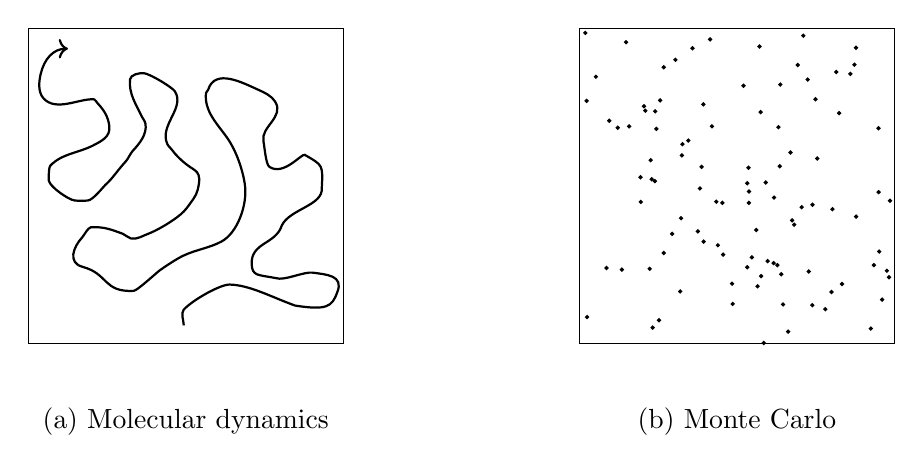
\begin{tikzpicture}
            \draw(0,0) rectangle (4,4);
            \begin{scope}[scale=0.17,shift={(-0.9,0)}]
                \draw [<-,thick]  (3.87,22) .. controls (2.75,22) and (2.09,21.21) .. (1.83,20.11) .. controls (1.71,19.6) and (1.6,18.77) .. (2.05,18.28) .. controls (2.99,17.27) and (4.71,18.29) .. (5.8,18.22) .. controls (5.89,18.21) and (6.06,17.94) .. (6.13,17.87) .. controls (6.57,17.39) and (6.87,16.92) .. (6.96,16.21) .. controls (7.05,15.4) and (6.34,15.09) .. (5.8,14.8) .. controls (4.74,14.23) and (3.4,14.17) .. (2.55,13.26) .. controls (2.41,13.11) and (2.43,12.16) .. (2.44,12.14) .. controls (2.54,11.66) and (3.92,10.71) .. (4.37,10.66) .. controls (4.7,10.63) and (5.03,10.63) .. (5.36,10.66) .. controls (5.75,10.7) and (6.49,11.67) .. (6.68,11.84) .. controls (7.25,12.36) and (7.6,12.95) .. (8.17,13.56) .. controls (8.38,13.78) and (8.51,14.16) .. (8.72,14.38) .. controls (9.2,14.9) and (9.79,15.6) .. (9.66,16.39) .. controls (9.62,16.61) and (9.41,16.85) .. (9.33,17.04) .. controls (8.93,17.89) and (8.41,18.64) .. (8.5,19.7) .. controls (8.53,20.07) and (9.23,20.21) .. (9.55,20.17) .. controls (10.02,20.11) and (11.68,19.1) .. (11.86,18.81) .. controls (12.59,17.64) and (10.9,16.44) .. (11.2,15.15) .. controls (11.3,14.71) and (11.45,14.7) .. (11.64,14.44) .. controls (11.95,14.02) and (12.28,13.71) .. (12.69,13.38) .. controls (13.4,12.81) and (13.9,12.91) .. (13.57,11.49) .. controls (13.51,11.22) and (13.39,11) .. (13.24,10.78) .. controls (13.01,10.46) and (12.79,10.12) .. (12.52,9.84) .. controls (12.01,9.29) and (10.52,8.41) .. (9.88,8.18) .. controls (9.47,8.04) and (9.01,7.71) .. (8.55,7.83) .. controls (8.33,7.89) and (8.17,8.1) .. (7.95,8.18) .. controls (7.08,8.49) and (6.59,8.71) .. (5.58,8.66) .. controls (5.36,8.64) and (5.07,8.05) .. (4.92,7.89) .. controls (4.28,7.2) and (3.81,6.01) .. (4.97,5.7) .. controls (6.91,5.18) and (6.5,3.79) .. (8.78,3.91) .. controls (9.05,3.93) and (10.52,5.3) .. (10.76,5.47) .. controls (11.25,5.8) and (11.91,6.26) .. (12.47,6.53) .. controls (13.43,6.99) and (14.41,7.1) .. (15.33,7.59) .. controls (16.55,8.25) and (17.26,10.33) .. (17.1,11.73) .. controls (16.96,12.88) and (16.44,14.38) .. (15.77,15.33) .. controls (15.04,16.37) and (14.03,17.33) .. (14.18,18.69) .. controls (14.18,18.72) and (14.32,18.88) .. (14.34,18.93) .. controls (14.85,20.57) and (16.93,19.45) .. (18.09,18.93) .. controls (18.53,18.73) and (19.07,18.5) .. (19.35,18.04) .. controls (20.06,16.91) and (18.25,16.15) .. (18.47,15.09) .. controls (18.55,14.73) and (18.65,13.35) .. (18.91,13.18) .. controls (19.96,12.45) and (21.34,14.2) .. (21.56,14.07) .. controls (22.89,13.29) and (22.93,13.37) .. (22.83,11.59) .. controls (22.94,10.29) and (20.46,10.03) .. (19.85,8.81) .. controls (19.41,7.38) and (17.54,7.55) .. (17.59,5.92) .. controls (17.65,5.01) and (17.98,5.13) .. (19.41,4.86) .. controls (20.02,4.64) and (21.52,5.37) .. (22.16,5.27) .. controls (23.1,5.13) and (24.53,5.09) .. (23.98,3.79) .. controls (23.6,2.73) and (23.21,2.44) .. (20.84,2.81) .. controls (19.08,3.44) and (17.44,4.35) .. (15.94,4.38) .. controls (15.28,4.4) and (13.22,3.26) .. (12.52,2.51) .. controls (12.28,2.26) and (12.52,1.64) .. (12.52,1.33) ;
            \end{scope}
            \node at (2,-1) {(a) Molecular dynamics};
            \begin{scope}[shift={(7,0)}]
                \draw (0,0) rectangle (4,4);
                \foreach \i in {0,...,100}{
                    \draw[fill=black] (rand*2+2,rand*2+2) circle (0.02);
                }
                \node at (2,-1) {(b) Monte Carlo};
            \end{scope}
        \end{tikzpicture}
        \caption{The difference between molecular dynamics and Monte Carlo.}
    \end{figure}

    \subsubsection{Inferential Statistics}
    A simple example. If you toss a coin 100 times and they all land heads. What do you think you will get if you flip it next time? We have done a fairly large number of experiments, so based on our sample, we would suspect that this coin is unfair, and we would still get a head next time. Now if you toss another coin for another 100 times, and you get 52 heads and 48 tails. The best estimate of the probability of getting a head for our next toss would be \(52\%\) based on our samples.

    \begin{law}[Strong law of large numbers (Kolmogorov's law)]
        Given a collection of independent and identically distributed (iid) samples from a random variable with finite mean, the sample average converges almost surely to the expected value.
        \begin{equation}
            \Prob\left(\lim_{n\to\infty}\overline{X}_n=\mu\right)=1\,.
        \end{equation}
    \end{law}
    What this means is that, as the number of trials \(n\) goes to infinity, the probability that the average of the observations converges to the expected value, is equal to one.\footnote{There is also a weak law of large numbers.
    \begin{law}[Weak law of large numbers (Khinchin's law)]
        The sample mean converges in probability to the expected value. That is, for any \(\epsilon>0\),
        \begin{equation}
            \lim_{n\to\infty}\Prob(\abs{\overline{X}_n-\mu}<\epsilon)=1\,.
        \end{equation}
    \end{law}
    This is not a maths course so we don't care about the difference here.}

    You might be worrying about some extreme events, like you are tossing a fair coin, but you get all heads for the first 100 tosses. But as you do more tosses, say 10,000 more tosses, you are likely to get around 5,000 heads with 5,000 tosses, and the extreme result of the first 100 tosses will be washed away. This is the \textit{regression to the mean}. Following an extreme event, the next random event will likely be less extreme.

    \subsubsection{Monte Carlo}
    Let's see an example of Monte Carlo in its simplest form. Consider a square of side length 2, and its inscribed circle. The area of the square is \(4\) and the area of the circle is \(\pi\). This means that if I randomly choose a point in the square, it has a chance
    \begin{equation}
        p=\frac{A_{\text{circle}}}{A_{\text{square}}}=\frac{\pi}{4}
    \end{equation}
    to fall inside the circle. Now if I am asking my computer to generate a random set of \(N\) points for some large enough \(N\), then the  fraction of points that will fall inside the circle will be
    \begin{equation}
        \lim_{N\to\infty}\frac{N_{\text{in}}}{N}=p=\frac{\pi}{4}\,.
    \end{equation}
    This means that by counting how many points are inside a circle, we can estimate the value of \(\pi\) by\footnote{I tried for \(N=1,000,000,000\) and it gives me an estimate of \(\pi\approx 3.141633\) in 7 minutes. Apparently this is not the most efficient way of calculating \(\pi\)}
    \begin{equation}
        \pi\simeq 4p=\frac{4N_{\text{in}}}{N}\,.
    \end{equation}
    We are essentially evaluating a 2D integral by the stochastic method.

    \begin{figure}
        \centering
        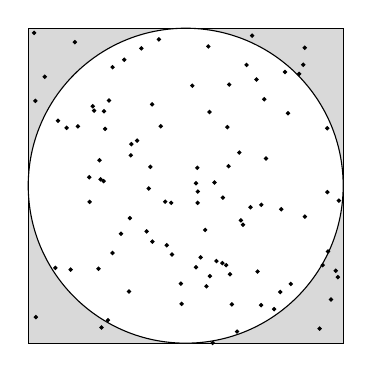
\begin{tikzpicture}
            \draw[fill=gray!30] (0,0) rectangle (4,4);
            \draw[fill=white] (2,2) circle (2);
            \foreach \i in {0,...,100}{
                \draw[fill=black] (rand*2+2,rand*2+2) circle (0.02);
            }
        \end{tikzpicture}
        \caption{Randomly generating \(N=100\) points in a square.}
    \end{figure}

    \subsection{Importance Sampling}
    As you can see in the above example, randomly sampling points from a uniform distribution may not be the most efficient way to perform an MC calculation.

    Suppose we are evaluating some integral
    \begin{equation}
        \int_{a}^{b}\dd{x}f(x)\,.
    \end{equation}
    If we want to do this using standard Monte Carlo, then we would sample points from \(a\) to \(b\) uniformly. However, if we are doing something like
    \begin{equation}
        \int_{-5}^{5}\dd{x}\ee^{-x^2}\,,
    \end{equation}
    which we know that most of the weight of the integral actually comes from a small range of \(x\) where \(f(x)\) is large. Sampling more often in that region should greatly increase the accuracy of the MC integration. However, this implies that we know something about \(f(x)\) already.

    \begin{figure}[ht!]
        \begin{subfigure}[h]{0.48\linewidth}
            \begin{adjustbox}{width=\linewidth}
            % This file was created with tikzplotlib v0.10.1.
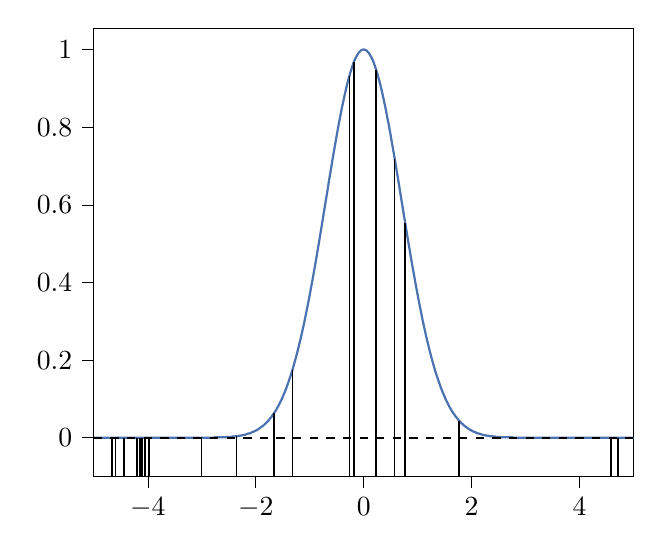
\begin{tikzpicture}

\definecolor{darkgray176}{RGB}{176,176,176}
\definecolor{steelblue76114176}{RGB}{76,114,176}

\begin{axis}[
tick align=outside,
tick pos=left,
x grid style={darkgray176},
xmin=-5, xmax=5,
xtick style={color=black},
y grid style={darkgray176},
ymin=-0.1, ymax=1.055,
ytick style={color=black}
]
\addplot [thick, steelblue76114176]
table {%
-5 0
-4.98 0
-4.96 0
-4.94 0
-4.92 0
-4.9 0
-4.88 0
-4.86 0
-4.84 0
-4.82 0
-4.8 0
-4.78 0
-4.76 0
-4.739 0
-4.719 0
-4.699 0
-4.679 0
-4.659 0
-4.639 0
-4.619 0
-4.599 0
-4.579 0
-4.559 0
-4.539 0
-4.519 0
-4.499 0
-4.479 0
-4.459 0
-4.439 0
-4.419 0
-4.399 0
-4.379 0
-4.359 0
-4.339 0
-4.319 0
-4.299 0
-4.279 0
-4.259 0
-4.238 0
-4.218 0
-4.198 0
-4.178 0
-4.158 0
-4.138 0
-4.118 0
-4.098 0
-4.078 0
-4.058 0
-4.038 0
-4.018 0
-3.998 0
-3.978 0
-3.958 0
-3.938 0
-3.918 0
-3.898 0
-3.878 0
-3.858 0
-3.838 0
-3.818 0
-3.798 0
-3.778 0
-3.758 0
-3.737 0
-3.717 0
-3.697 0
-3.677 0
-3.657 0
-3.637 0
-3.617 0
-3.597 0
-3.577 0
-3.557 0
-3.537 0
-3.517 0
-3.497 0
-3.477 0
-3.457 0
-3.437 0
-3.417 0
-3.397 0
-3.377 0
-3.357 0
-3.337 0
-3.317 0
-3.297 0
-3.277 0
-3.257 0
-3.236 0
-3.216 0
-3.196 0
-3.176 0
-3.156 0
-3.136 0
-3.116 0
-3.096 0
-3.076 0
-3.056 0
-3.036 0
-3.016 0
-2.996 0
-2.976 0
-2.956 0
-2.936 0
-2.916 0
-2.896 0
-2.876 0
-2.856 0
-2.836 0
-2.816 0
-2.796 0
-2.776 0
-2.756 0.001
-2.735 0.001
-2.715 0.001
-2.695 0.001
-2.675 0.001
-2.655 0.001
-2.635 0.001
-2.615 0.001
-2.595 0.001
-2.575 0.001
-2.555 0.001
-2.535 0.002
-2.515 0.002
-2.495 0.002
-2.475 0.002
-2.455 0.002
-2.435 0.003
-2.415 0.003
-2.395 0.003
-2.375 0.004
-2.355 0.004
-2.335 0.004
-2.315 0.005
-2.295 0.005
-2.275 0.006
-2.255 0.006
-2.234 0.007
-2.214 0.007
-2.194 0.008
-2.174 0.009
-2.154 0.01
-2.134 0.011
-2.114 0.011
-2.094 0.012
-2.074 0.014
-2.054 0.015
-2.034 0.016
-2.014 0.017
-1.994 0.019
-1.974 0.02
-1.954 0.022
-1.934 0.024
-1.914 0.026
-1.894 0.028
-1.874 0.03
-1.854 0.032
-1.834 0.035
-1.814 0.037
-1.794 0.04
-1.774 0.043
-1.754 0.046
-1.733 0.05
-1.713 0.053
-1.693 0.057
-1.673 0.061
-1.653 0.065
-1.633 0.069
-1.613 0.074
-1.593 0.079
-1.573 0.084
-1.553 0.09
-1.533 0.095
-1.513 0.101
-1.493 0.108
-1.473 0.114
-1.453 0.121
-1.433 0.128
-1.413 0.136
-1.393 0.144
-1.373 0.152
-1.353 0.16
-1.333 0.169
-1.313 0.178
-1.293 0.188
-1.273 0.198
-1.253 0.208
-1.232 0.219
-1.212 0.23
-1.192 0.242
-1.172 0.253
-1.152 0.265
-1.132 0.278
-1.112 0.29
-1.092 0.303
-1.072 0.317
-1.052 0.331
-1.032 0.345
-1.012 0.359
-0.992 0.374
-0.972 0.389
-0.952 0.404
-0.932 0.42
-0.912 0.435
-0.892 0.451
-0.872 0.467
-0.852 0.484
-0.832 0.5
-0.812 0.517
-0.792 0.534
-0.772 0.551
-0.752 0.568
-0.731 0.586
-0.711 0.603
-0.691 0.62
-0.671 0.637
-0.651 0.655
-0.631 0.672
-0.611 0.688
-0.591 0.705
-0.571 0.722
-0.551 0.738
-0.531 0.754
-0.511 0.77
-0.491 0.786
-0.471 0.801
-0.451 0.816
-0.431 0.83
-0.411 0.845
-0.391 0.858
-0.371 0.871
-0.351 0.884
-0.331 0.896
-0.311 0.908
-0.291 0.919
-0.271 0.929
-0.251 0.939
-0.23 0.948
-0.21 0.957
-0.19 0.965
-0.17 0.972
-0.15 0.978
-0.13 0.983
-0.11 0.988
-0.09 0.992
-0.07 0.995
-0.05 0.998
-0.03 0.999
-0.01 1
0.01 1
0.03 0.999
0.05 0.998
0.07 0.995
0.09 0.992
0.11 0.988
0.13 0.983
0.15 0.978
0.17 0.972
0.19 0.965
0.21 0.957
0.23 0.948
0.251 0.939
0.271 0.929
0.291 0.919
0.311 0.908
0.331 0.896
0.351 0.884
0.371 0.871
0.391 0.858
0.411 0.845
0.431 0.83
0.451 0.816
0.471 0.801
0.491 0.786
0.511 0.77
0.531 0.754
0.551 0.738
0.571 0.722
0.591 0.705
0.611 0.688
0.631 0.672
0.651 0.655
0.671 0.637
0.691 0.62
0.711 0.603
0.731 0.586
0.752 0.568
0.772 0.551
0.792 0.534
0.812 0.517
0.832 0.5
0.852 0.484
0.872 0.467
0.892 0.451
0.912 0.435
0.932 0.42
0.952 0.404
0.972 0.389
0.992 0.374
1.012 0.359
1.032 0.345
1.052 0.331
1.072 0.317
1.092 0.303
1.112 0.29
1.132 0.278
1.152 0.265
1.172 0.253
1.192 0.242
1.212 0.23
1.232 0.219
1.253 0.208
1.273 0.198
1.293 0.188
1.313 0.178
1.333 0.169
1.353 0.16
1.373 0.152
1.393 0.144
1.413 0.136
1.433 0.128
1.453 0.121
1.473 0.114
1.493 0.108
1.513 0.101
1.533 0.095
1.553 0.09
1.573 0.084
1.593 0.079
1.613 0.074
1.633 0.069
1.653 0.065
1.673 0.061
1.693 0.057
1.713 0.053
1.733 0.05
1.754 0.046
1.774 0.043
1.794 0.04
1.814 0.037
1.834 0.035
1.854 0.032
1.874 0.03
1.894 0.028
1.914 0.026
1.934 0.024
1.954 0.022
1.974 0.02
1.994 0.019
2.014 0.017
2.034 0.016
2.054 0.015
2.074 0.014
2.094 0.012
2.114 0.011
2.134 0.011
2.154 0.01
2.174 0.009
2.194 0.008
2.214 0.007
2.234 0.007
2.255 0.006
2.275 0.006
2.295 0.005
2.315 0.005
2.335 0.004
2.355 0.004
2.375 0.004
2.395 0.003
2.415 0.003
2.435 0.003
2.455 0.002
2.475 0.002
2.495 0.002
2.515 0.002
2.535 0.002
2.555 0.001
2.575 0.001
2.595 0.001
2.615 0.001
2.635 0.001
2.655 0.001
2.675 0.001
2.695 0.001
2.715 0.001
2.735 0.001
2.756 0.001
2.776 0
2.796 0
2.816 0
2.836 0
2.856 0
2.876 0
2.896 0
2.916 0
2.936 0
2.956 0
2.976 0
2.996 0
3.016 0
3.036 0
3.056 0
3.076 0
3.096 0
3.116 0
3.136 0
3.156 0
3.176 0
3.196 0
3.216 0
3.236 0
3.257 0
3.277 0
3.297 0
3.317 0
3.337 0
3.357 0
3.377 0
3.397 0
3.417 0
3.437 0
3.457 0
3.477 0
3.497 0
3.517 0
3.537 0
3.557 0
3.577 0
3.597 0
3.617 0
3.637 0
3.657 0
3.677 0
3.697 0
3.717 0
3.737 0
3.758 0
3.778 0
3.798 0
3.818 0
3.838 0
3.858 0
3.878 0
3.898 0
3.918 0
3.938 0
3.958 0
3.978 0
3.998 0
4.018 0
4.038 0
4.058 0
4.078 0
4.098 0
4.118 0
4.138 0
4.158 0
4.178 0
4.198 0
4.218 0
4.238 0
4.259 0
4.279 0
4.299 0
4.319 0
4.339 0
4.359 0
4.379 0
4.399 0
4.419 0
4.439 0
4.459 0
4.479 0
4.499 0
4.519 0
4.539 0
4.559 0
4.579 0
4.599 0
4.619 0
4.639 0
4.659 0
4.679 0
4.699 0
4.719 0
4.739 0
4.76 0
4.78 0
4.8 0
4.82 0
4.84 0
4.86 0
4.88 0
4.9 0
4.92 0
4.94 0
4.96 0
4.98 0
5 0
};
\addplot [semithick, black]
table {%
-4.66 -0.1
-4.66 0
};
\addplot [semithick, black]
table {%
-4.601 -0.1
-4.601 0
};
\addplot [semithick, black]
table {%
-4.446 -0.1
-4.446 0
};
\addplot [semithick, black]
table {%
-4.202 -0.1
-4.202 0
};
\addplot [semithick, black]
table {%
-4.142 -0.1
-4.142 0
};
\addplot [semithick, black]
table {%
-4.106 -0.1
-4.106 0
};
\addplot [semithick, black]
table {%
-4.054 -0.1
-4.054 0
};
\addplot [semithick, black]
table {%
-3.981 -0.1
-3.981 0
};
\addplot [semithick, black]
table {%
-3.005 -0.1
-3.005 0
};
\addplot [semithick, black]
table {%
-2.358 -0.1
-2.358 0.004
};
\addplot [semithick, black]
table {%
-1.663 -0.1
-1.663 0.063
};
\addplot [semithick, black]
table {%
-1.32 -0.1
-1.32 0.175
};
\addplot [semithick, black]
table {%
-0.263 -0.1
-0.263 0.933
};
\addplot [semithick, black]
table {%
-0.178 -0.1
-0.178 0.969
};
\addplot [semithick, black]
table {%
0.231 -0.1
0.231 0.948
};
\addplot [semithick, black]
table {%
0.574 -0.1
0.574 0.719
};
\addplot [semithick, black]
table {%
0.769 -0.1
0.769 0.553
};
\addplot [semithick, black]
table {%
1.769 -0.1
1.769 0.044
};
\addplot [semithick, black]
table {%
4.583 -0.1
4.583 0
};
\addplot [semithick, black]
table {%
4.717 -0.1
4.717 0
};
\addplot [semithick, dashed, black]
table {%
-5  0
5   0
};
\end{axis}

\end{tikzpicture}

            \end{adjustbox}
            \caption{Sampling with uniform distribution.}
        \end{subfigure}
        \hfill
        \begin{subfigure}[h]{0.48\linewidth}
            \begin{adjustbox}{width=\linewidth}
            % This file was created with tikzplotlib v0.10.1.
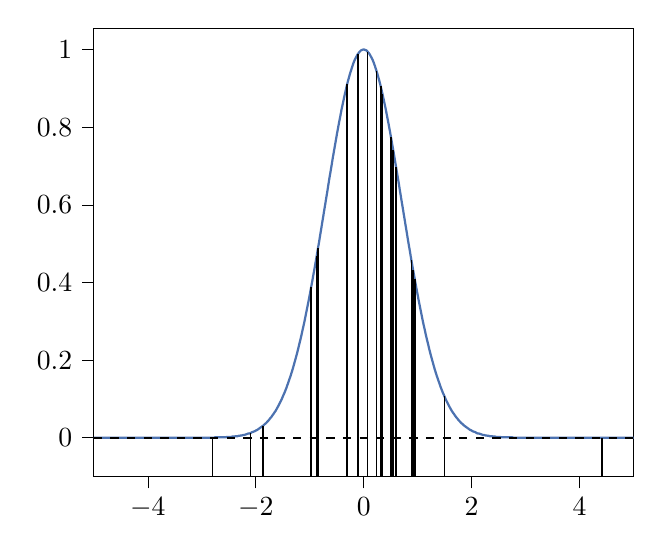
\begin{tikzpicture}

\definecolor{darkgray176}{RGB}{176,176,176}
\definecolor{steelblue76114176}{RGB}{76,114,176}

\begin{axis}[
tick align=outside,
tick pos=left,
x grid style={darkgray176},
xmin=-5, xmax=5,
xtick style={color=black},
y grid style={darkgray176},
ymin=-0.1, ymax=1.055,
ytick style={color=black}
]
\addplot [thick, steelblue76114176]
table {%
-5 0
-4.98 0
-4.96 0
-4.94 0
-4.92 0
-4.9 0
-4.88 0
-4.86 0
-4.84 0
-4.82 0
-4.8 0
-4.78 0
-4.76 0
-4.739 0
-4.719 0
-4.699 0
-4.679 0
-4.659 0
-4.639 0
-4.619 0
-4.599 0
-4.579 0
-4.559 0
-4.539 0
-4.519 0
-4.499 0
-4.479 0
-4.459 0
-4.439 0
-4.419 0
-4.399 0
-4.379 0
-4.359 0
-4.339 0
-4.319 0
-4.299 0
-4.279 0
-4.259 0
-4.238 0
-4.218 0
-4.198 0
-4.178 0
-4.158 0
-4.138 0
-4.118 0
-4.098 0
-4.078 0
-4.058 0
-4.038 0
-4.018 0
-3.998 0
-3.978 0
-3.958 0
-3.938 0
-3.918 0
-3.898 0
-3.878 0
-3.858 0
-3.838 0
-3.818 0
-3.798 0
-3.778 0
-3.758 0
-3.737 0
-3.717 0
-3.697 0
-3.677 0
-3.657 0
-3.637 0
-3.617 0
-3.597 0
-3.577 0
-3.557 0
-3.537 0
-3.517 0
-3.497 0
-3.477 0
-3.457 0
-3.437 0
-3.417 0
-3.397 0
-3.377 0
-3.357 0
-3.337 0
-3.317 0
-3.297 0
-3.277 0
-3.257 0
-3.236 0
-3.216 0
-3.196 0
-3.176 0
-3.156 0
-3.136 0
-3.116 0
-3.096 0
-3.076 0
-3.056 0
-3.036 0
-3.016 0
-2.996 0
-2.976 0
-2.956 0
-2.936 0
-2.916 0
-2.896 0
-2.876 0
-2.856 0
-2.836 0
-2.816 0
-2.796 0
-2.776 0
-2.756 0.001
-2.735 0.001
-2.715 0.001
-2.695 0.001
-2.675 0.001
-2.655 0.001
-2.635 0.001
-2.615 0.001
-2.595 0.001
-2.575 0.001
-2.555 0.001
-2.535 0.002
-2.515 0.002
-2.495 0.002
-2.475 0.002
-2.455 0.002
-2.435 0.003
-2.415 0.003
-2.395 0.003
-2.375 0.004
-2.355 0.004
-2.335 0.004
-2.315 0.005
-2.295 0.005
-2.275 0.006
-2.255 0.006
-2.234 0.007
-2.214 0.007
-2.194 0.008
-2.174 0.009
-2.154 0.01
-2.134 0.011
-2.114 0.011
-2.094 0.012
-2.074 0.014
-2.054 0.015
-2.034 0.016
-2.014 0.017
-1.994 0.019
-1.974 0.02
-1.954 0.022
-1.934 0.024
-1.914 0.026
-1.894 0.028
-1.874 0.03
-1.854 0.032
-1.834 0.035
-1.814 0.037
-1.794 0.04
-1.774 0.043
-1.754 0.046
-1.733 0.05
-1.713 0.053
-1.693 0.057
-1.673 0.061
-1.653 0.065
-1.633 0.069
-1.613 0.074
-1.593 0.079
-1.573 0.084
-1.553 0.09
-1.533 0.095
-1.513 0.101
-1.493 0.108
-1.473 0.114
-1.453 0.121
-1.433 0.128
-1.413 0.136
-1.393 0.144
-1.373 0.152
-1.353 0.16
-1.333 0.169
-1.313 0.178
-1.293 0.188
-1.273 0.198
-1.253 0.208
-1.232 0.219
-1.212 0.23
-1.192 0.242
-1.172 0.253
-1.152 0.265
-1.132 0.278
-1.112 0.29
-1.092 0.303
-1.072 0.317
-1.052 0.331
-1.032 0.345
-1.012 0.359
-0.992 0.374
-0.972 0.389
-0.952 0.404
-0.932 0.42
-0.912 0.435
-0.892 0.451
-0.872 0.467
-0.852 0.484
-0.832 0.5
-0.812 0.517
-0.792 0.534
-0.772 0.551
-0.752 0.568
-0.731 0.586
-0.711 0.603
-0.691 0.62
-0.671 0.637
-0.651 0.655
-0.631 0.672
-0.611 0.688
-0.591 0.705
-0.571 0.722
-0.551 0.738
-0.531 0.754
-0.511 0.77
-0.491 0.786
-0.471 0.801
-0.451 0.816
-0.431 0.83
-0.411 0.845
-0.391 0.858
-0.371 0.871
-0.351 0.884
-0.331 0.896
-0.311 0.908
-0.291 0.919
-0.271 0.929
-0.251 0.939
-0.23 0.948
-0.21 0.957
-0.19 0.965
-0.17 0.972
-0.15 0.978
-0.13 0.983
-0.11 0.988
-0.09 0.992
-0.07 0.995
-0.05 0.998
-0.03 0.999
-0.01 1
0.01 1
0.03 0.999
0.05 0.998
0.07 0.995
0.09 0.992
0.11 0.988
0.13 0.983
0.15 0.978
0.17 0.972
0.19 0.965
0.21 0.957
0.23 0.948
0.251 0.939
0.271 0.929
0.291 0.919
0.311 0.908
0.331 0.896
0.351 0.884
0.371 0.871
0.391 0.858
0.411 0.845
0.431 0.83
0.451 0.816
0.471 0.801
0.491 0.786
0.511 0.77
0.531 0.754
0.551 0.738
0.571 0.722
0.591 0.705
0.611 0.688
0.631 0.672
0.651 0.655
0.671 0.637
0.691 0.62
0.711 0.603
0.731 0.586
0.752 0.568
0.772 0.551
0.792 0.534
0.812 0.517
0.832 0.5
0.852 0.484
0.872 0.467
0.892 0.451
0.912 0.435
0.932 0.42
0.952 0.404
0.972 0.389
0.992 0.374
1.012 0.359
1.032 0.345
1.052 0.331
1.072 0.317
1.092 0.303
1.112 0.29
1.132 0.278
1.152 0.265
1.172 0.253
1.192 0.242
1.212 0.23
1.232 0.219
1.253 0.208
1.273 0.198
1.293 0.188
1.313 0.178
1.333 0.169
1.353 0.16
1.373 0.152
1.393 0.144
1.413 0.136
1.433 0.128
1.453 0.121
1.473 0.114
1.493 0.108
1.513 0.101
1.533 0.095
1.553 0.09
1.573 0.084
1.593 0.079
1.613 0.074
1.633 0.069
1.653 0.065
1.673 0.061
1.693 0.057
1.713 0.053
1.733 0.05
1.754 0.046
1.774 0.043
1.794 0.04
1.814 0.037
1.834 0.035
1.854 0.032
1.874 0.03
1.894 0.028
1.914 0.026
1.934 0.024
1.954 0.022
1.974 0.02
1.994 0.019
2.014 0.017
2.034 0.016
2.054 0.015
2.074 0.014
2.094 0.012
2.114 0.011
2.134 0.011
2.154 0.01
2.174 0.009
2.194 0.008
2.214 0.007
2.234 0.007
2.255 0.006
2.275 0.006
2.295 0.005
2.315 0.005
2.335 0.004
2.355 0.004
2.375 0.004
2.395 0.003
2.415 0.003
2.435 0.003
2.455 0.002
2.475 0.002
2.495 0.002
2.515 0.002
2.535 0.002
2.555 0.001
2.575 0.001
2.595 0.001
2.615 0.001
2.635 0.001
2.655 0.001
2.675 0.001
2.695 0.001
2.715 0.001
2.735 0.001
2.756 0.001
2.776 0
2.796 0
2.816 0
2.836 0
2.856 0
2.876 0
2.896 0
2.916 0
2.936 0
2.956 0
2.976 0
2.996 0
3.016 0
3.036 0
3.056 0
3.076 0
3.096 0
3.116 0
3.136 0
3.156 0
3.176 0
3.196 0
3.216 0
3.236 0
3.257 0
3.277 0
3.297 0
3.317 0
3.337 0
3.357 0
3.377 0
3.397 0
3.417 0
3.437 0
3.457 0
3.477 0
3.497 0
3.517 0
3.537 0
3.557 0
3.577 0
3.597 0
3.617 0
3.637 0
3.657 0
3.677 0
3.697 0
3.717 0
3.737 0
3.758 0
3.778 0
3.798 0
3.818 0
3.838 0
3.858 0
3.878 0
3.898 0
3.918 0
3.938 0
3.958 0
3.978 0
3.998 0
4.018 0
4.038 0
4.058 0
4.078 0
4.098 0
4.118 0
4.138 0
4.158 0
4.178 0
4.198 0
4.218 0
4.238 0
4.259 0
4.279 0
4.299 0
4.319 0
4.339 0
4.359 0
4.379 0
4.399 0
4.419 0
4.439 0
4.459 0
4.479 0
4.499 0
4.519 0
4.539 0
4.559 0
4.579 0
4.599 0
4.619 0
4.639 0
4.659 0
4.679 0
4.699 0
4.719 0
4.739 0
4.76 0
4.78 0
4.8 0
4.82 0
4.84 0
4.86 0
4.88 0
4.9 0
4.92 0
4.94 0
4.96 0
4.98 0
5 0
};
\addplot [semithick, black]
table {%
-2.799 -0.1
-2.799 0
};
\addplot [semithick, black]
table {%
-2.097 -0.1
-2.097 0.012
};
\addplot [semithick, black]
table {%
-1.862 -0.1
-1.862 0.031
};
\addplot [semithick, black]
table {%
-0.971 -0.1
-0.971 0.389
};
\addplot [semithick, black]
table {%
-0.872 -0.1
-0.872 0.467
};
\addplot [semithick, black]
table {%
-0.846 -0.1
-0.846 0.489
};
\addplot [semithick, black]
table {%
-0.304 -0.1
-0.304 0.912
};
\addplot [semithick, black]
table {%
-0.107 -0.1
-0.107 0.989
};
\addplot [semithick, black]
table {%
0.07 -0.1
0.07 0.995
};
\addplot [semithick, black]
table {%
0.239 -0.1
0.239 0.945
};
\addplot [semithick, black]
table {%
0.315 -0.1
0.315 0.906
};
\addplot [semithick, black]
table {%
0.35 -0.1
0.35 0.885
};
\addplot [semithick, black]
table {%
0.505 -0.1
0.505 0.775
};
\addplot [semithick, black]
table {%
0.546 -0.1
0.546 0.742
};
\addplot [semithick, black]
table {%
0.601 -0.1
0.601 0.697
};
\addplot [semithick, black]
table {%
0.883 -0.1
0.883 0.458
};
\addplot [semithick, black]
table {%
0.917 -0.1
0.917 0.431
};
\addplot [semithick, black]
table {%
0.945 -0.1
0.945 0.41
};
\addplot [semithick, black]
table {%
1.496 -0.1
1.496 0.107
};
\addplot [semithick, black]
table {%
4.418 -0.1
4.418 0
};
\addplot [semithick, dashed, black]
table {%
-5  0
5   0
};
\end{axis}

\end{tikzpicture}

            \end{adjustbox}
            \caption{Sampling with biased distribution}
        \end{subfigure}%
        \caption{Monte Carlo method to evaluate the integral \(\int_{-5}^{5}\dd{x}\ee^{-x^2}\) using uniform and biased sampling.}
    \end{figure}
    \begin{figure}[ht!]
        \centering
        % This file was created with tikzplotlib v0.10.1.
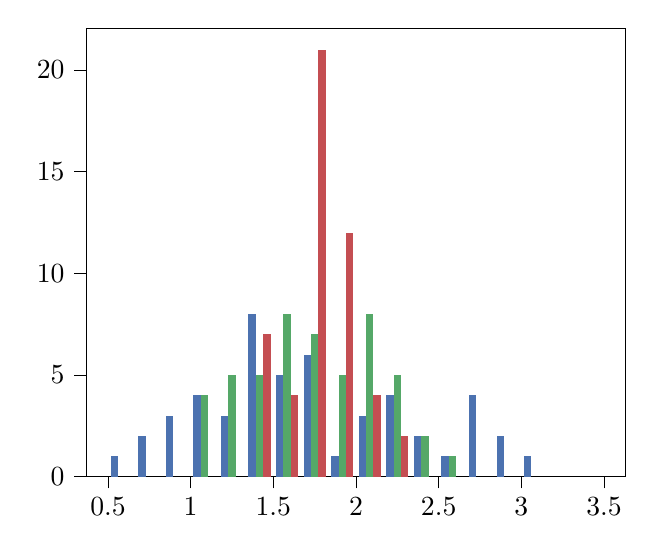
\begin{tikzpicture}

\definecolor{darkgray176}{RGB}{176,176,176}
\definecolor{indianred1967882}{RGB}{196,78,82}
\definecolor{mediumseagreen85168104}{RGB}{85,168,104}
\definecolor{steelblue76114176}{RGB}{76,114,176}

\begin{axis}[
tick align=outside,
tick pos=left,
x grid style={darkgray176},
xmin=0.368333333333333, xmax=3.63166666666667,
xtick style={color=black},
y grid style={darkgray176},
ymin=0, ymax=22.05,
ytick style={color=black}
]
\draw[draw=none,fill=steelblue76114176] (axis cs:0.516666666666667,0) rectangle (axis cs:0.561111111111111,1);
\draw[draw=none,fill=steelblue76114176] (axis cs:0.683333333333333,0) rectangle (axis cs:0.727777777777778,2);
\draw[draw=none,fill=steelblue76114176] (axis cs:0.85,0) rectangle (axis cs:0.894444444444444,3);
\draw[draw=none,fill=steelblue76114176] (axis cs:1.01666666666667,0) rectangle (axis cs:1.06111111111111,4);
\draw[draw=none,fill=steelblue76114176] (axis cs:1.18333333333333,0) rectangle (axis cs:1.22777777777778,3);
\draw[draw=none,fill=steelblue76114176] (axis cs:1.35,0) rectangle (axis cs:1.39444444444444,8);
\draw[draw=none,fill=steelblue76114176] (axis cs:1.51666666666667,0) rectangle (axis cs:1.56111111111111,5);
\draw[draw=none,fill=steelblue76114176] (axis cs:1.68333333333333,0) rectangle (axis cs:1.72777777777778,6);
\draw[draw=none,fill=steelblue76114176] (axis cs:1.85,0) rectangle (axis cs:1.89444444444444,1);
\draw[draw=none,fill=steelblue76114176] (axis cs:2.01666666666667,0) rectangle (axis cs:2.06111111111111,3);
\draw[draw=none,fill=steelblue76114176] (axis cs:2.18333333333333,0) rectangle (axis cs:2.22777777777778,4);
\draw[draw=none,fill=steelblue76114176] (axis cs:2.35,0) rectangle (axis cs:2.39444444444444,2);
\draw[draw=none,fill=steelblue76114176] (axis cs:2.51666666666667,0) rectangle (axis cs:2.56111111111111,1);
\draw[draw=none,fill=steelblue76114176] (axis cs:2.68333333333333,0) rectangle (axis cs:2.72777777777778,4);
\draw[draw=none,fill=steelblue76114176] (axis cs:2.85,0) rectangle (axis cs:2.89444444444444,2);
\draw[draw=none,fill=steelblue76114176] (axis cs:3.01666666666667,0) rectangle (axis cs:3.06111111111111,1);
\draw[draw=none,fill=steelblue76114176] (axis cs:3.18333333333333,0) rectangle (axis cs:3.22777777777778,0);
\draw[draw=none,fill=steelblue76114176] (axis cs:3.35,0) rectangle (axis cs:3.39444444444444,0);
\draw[draw=none,fill=mediumseagreen85168104] (axis cs:0.561111111111111,0) rectangle (axis cs:0.605555555555556,0);
\draw[draw=none,fill=mediumseagreen85168104] (axis cs:0.727777777777778,0) rectangle (axis cs:0.772222222222222,0);
\draw[draw=none,fill=mediumseagreen85168104] (axis cs:0.894444444444444,0) rectangle (axis cs:0.938888888888889,0);
\draw[draw=none,fill=mediumseagreen85168104] (axis cs:1.06111111111111,0) rectangle (axis cs:1.10555555555556,4);
\draw[draw=none,fill=mediumseagreen85168104] (axis cs:1.22777777777778,0) rectangle (axis cs:1.27222222222222,5);
\draw[draw=none,fill=mediumseagreen85168104] (axis cs:1.39444444444444,0) rectangle (axis cs:1.43888888888889,5);
\draw[draw=none,fill=mediumseagreen85168104] (axis cs:1.56111111111111,0) rectangle (axis cs:1.60555555555556,8);
\draw[draw=none,fill=mediumseagreen85168104] (axis cs:1.72777777777778,0) rectangle (axis cs:1.77222222222222,7);
\draw[draw=none,fill=mediumseagreen85168104] (axis cs:1.89444444444444,0) rectangle (axis cs:1.93888888888889,5);
\draw[draw=none,fill=mediumseagreen85168104] (axis cs:2.06111111111111,0) rectangle (axis cs:2.10555555555556,8);
\draw[draw=none,fill=mediumseagreen85168104] (axis cs:2.22777777777778,0) rectangle (axis cs:2.27222222222222,5);
\draw[draw=none,fill=mediumseagreen85168104] (axis cs:2.39444444444444,0) rectangle (axis cs:2.43888888888889,2);
\draw[draw=none,fill=mediumseagreen85168104] (axis cs:2.56111111111111,0) rectangle (axis cs:2.60555555555556,1);
\draw[draw=none,fill=mediumseagreen85168104] (axis cs:2.72777777777778,0) rectangle (axis cs:2.77222222222222,0);
\draw[draw=none,fill=mediumseagreen85168104] (axis cs:2.89444444444444,0) rectangle (axis cs:2.93888888888889,0);
\draw[draw=none,fill=mediumseagreen85168104] (axis cs:3.06111111111111,0) rectangle (axis cs:3.10555555555556,0);
\draw[draw=none,fill=mediumseagreen85168104] (axis cs:3.22777777777778,0) rectangle (axis cs:3.27222222222222,0);
\draw[draw=none,fill=mediumseagreen85168104] (axis cs:3.39444444444444,0) rectangle (axis cs:3.43888888888889,0);
\draw[draw=none,fill=indianred1967882] (axis cs:0.605555555555556,0) rectangle (axis cs:0.65,0);
\draw[draw=none,fill=indianred1967882] (axis cs:0.772222222222222,0) rectangle (axis cs:0.816666666666667,0);
\draw[draw=none,fill=indianred1967882] (axis cs:0.938888888888889,0) rectangle (axis cs:0.983333333333333,0);
\draw[draw=none,fill=indianred1967882] (axis cs:1.10555555555556,0) rectangle (axis cs:1.15,0);
\draw[draw=none,fill=indianred1967882] (axis cs:1.27222222222222,0) rectangle (axis cs:1.31666666666667,0);
\draw[draw=none,fill=indianred1967882] (axis cs:1.43888888888889,0) rectangle (axis cs:1.48333333333333,7);
\draw[draw=none,fill=indianred1967882] (axis cs:1.60555555555556,0) rectangle (axis cs:1.65,4);
\draw[draw=none,fill=indianred1967882] (axis cs:1.77222222222222,0) rectangle (axis cs:1.81666666666667,21);
\draw[draw=none,fill=indianred1967882] (axis cs:1.93888888888889,0) rectangle (axis cs:1.98333333333333,12);
\draw[draw=none,fill=indianred1967882] (axis cs:2.10555555555556,0) rectangle (axis cs:2.15,4);
\draw[draw=none,fill=indianred1967882] (axis cs:2.27222222222222,0) rectangle (axis cs:2.31666666666667,2);
\draw[draw=none,fill=indianred1967882] (axis cs:2.43888888888889,0) rectangle (axis cs:2.48333333333333,0);
\draw[draw=none,fill=indianred1967882] (axis cs:2.60555555555556,0) rectangle (axis cs:2.65,0);
\draw[draw=none,fill=indianred1967882] (axis cs:2.77222222222222,0) rectangle (axis cs:2.81666666666667,0);
\draw[draw=none,fill=indianred1967882] (axis cs:2.93888888888889,0) rectangle (axis cs:2.98333333333333,0);
\draw[draw=none,fill=indianred1967882] (axis cs:3.10555555555556,0) rectangle (axis cs:3.15,0);
\draw[draw=none,fill=indianred1967882] (axis cs:3.27222222222222,0) rectangle (axis cs:3.31666666666667,0);
\draw[draw=none,fill=indianred1967882] (axis cs:3.43888888888889,0) rectangle (axis cs:3.48333333333333,0);
\end{axis}

\end{tikzpicture}

        \caption{The histogram of 50 attempts to evaluate the integral \(\int_{-5}^{5}\dd{x}\ee^{-x^2}=\sqrt{\pi}\erf(5)\approx 1.77245\) using uniform (blue), biased (green) and an even more biased (red) sampling. The uniform sampling gives \(1.73\pm 0.64\), the biased sampling gives \(1.75\pm 0.39\) and the more biased sampling gives \(1.78\pm 0.19\). All three sampling methods give correct results on average due to a fairly large number of attempts (law of large numbers), but a more biased sampling gives a more consistent result.}
    \end{figure}

    To do this, we sample from a biased probability distribution \(w(x)\), which is derived from the best guess of what the function \(f(x)\) will look like. An estimate of the integral can then be written as
    \begin{equation}
        I=\frac{1}{N}\sum_{i=1}^{N}\frac{f(x_{i\mid w})}{w(x_{i\mid w})}\,,
    \end{equation}
    where \(x_{i\mid w}\) means that \(x_i\) is drawn from the probability distribution \(w(x)\), \(x_{i}\sim w(x)\). Here the division by \(w(x_{i\mid w})\) is to compensate for biasing the distribution. When \(w(x_{i\mid w})\) is a uniform distribution, we recover the uniform sampling.

    The variance of our integral estimation is
    \begin{equation}
        \sigma_{I\mid w}^2=\frac{1}{N}\eval{\frac{1}{N}\sum_{i=1}^{N}\left(\frac{f(x_{i\mid w})}{w(x_{i\mid w})}-\eval{\frac{f(x_{i\mid w})}{w(x_{i\mid w})}}\right)^2}=\frac{1}{N}\eval{\sigma_{f\mid w}^2}\,.
    \end{equation}
    The error still scales as \(N^{-1/2}\) but the prefactor is different for different sampling. The best prefactor would result from using
    \begin{equation}
        w(x)=\frac{1}{\mathcal{I}}f(x)\,,
    \end{equation}
    where \(\mathcal{I}=\int_{a}^{b}\dd{x}f(x)\) is for normalisation, for which \(\sigma_{f\mid w}=0\). In this case our estimation would always be exact, but this requires us to know the integral \textit{a priori}. Hence, in practice, we can only have a good estimate of what a suitable \(w(x)\) might be. Choosing a distribution that gives a good estimate for \(w(x)\) is known as \textit{importance sampling}. This is a crucial step in MC calculation. When sampling highly non-uniform functions, brute force MC with uniform sampling can result in a very large pre-factor for \(\sigma_{I\mid w}\).

    \subsubsection{Importance Sampling in Statistical Mechanics}
    Importance sampling is extremely crucial in statistical mechanical systems since it involves high dimensional integrals with significant contributions from only a very small fraction of the total possible sampling spaces.

    For example, suppose we want to evaluate the ensemble average of a physical quantity \(A\)
    \begin{equation}
        \eval{A}=\sum_{\ket{n}} A_n p_n=\frac{1}{Q}\sum_{\ket{n}} A_n \ee^{-\beta E_n}\,,
    \end{equation}
    where \(A_n\) is the value of the quantity \(A\) for the microstate \(\ket{n}\), and the sum is taken over all possible microstates. To evaluate this using Monte Carlo, the simplest way is to choose \(M\) states completely randomly and take the average with the Boltzmann factor
    \begin{equation}
        A_M=\frac{\sum_{\ket{n}}^{M}A_n \ee^{-\beta E_n}}{\sum_{\ket{n}}^{M}\ee^{-\beta E_n}}\,,
    \end{equation}
    which is analogous to the random uniform sampling we discussed in the context of integrals. In theory, as \(M\to\infty\) (or to the number of all possible microstates if this is finite), then \(A_M\to \eval{A}\). But in practice there are two major problems.
    \begin{enumerate}[topsep=0pt]
        \item The number of states in a statistical mechanical system usually grows exponentially with system size.
        
        For example, consider an \(N\times N\) 2D Ising lattice, where each lattice point can sit in \(S_i=\pm 1\). The total number of states is \(2^{N^2}\). Even a \(5\times 5\) lattice will have \(2^{25}=33,554,432\) distinct states. Doubling each side to a \(10\times 10\) lattice, this number will grow to \(10^{30}\). The number will soon get astronomically large, and it will get extremely difficult to sample a proper fraction of it.
        \item Averages are typically dominated by a very small fraction of the states, which random uniform sampling is very unlikely to find.
        
        Consider a hard-sphere liquid. If you locate the particles randomly, then you will easily get particles overlapping with each other, even at moderate particle density. Such situation gives infinite energy and so contribute nothing to the average \(\eval{A}\). For example, if we simulate 100 hard-spheres near the freezing transition, then only one in about \(10^{260}\) random configurations would count towards the average.

        \begin{figure}[ht!]
            \centering
            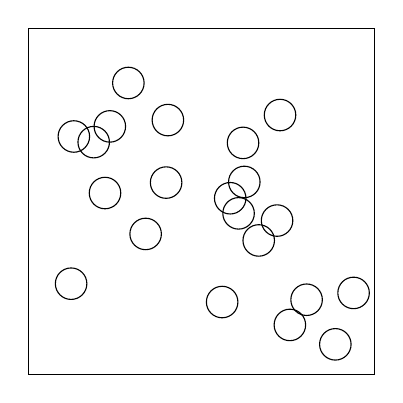
\begin{tikzpicture}
                \draw (-0.2,-0.2) rectangle (4.2,4.2);
                \foreach \i in {0,...,20}{
                    \draw (rand*2+2,rand*2+2) circle (0.2);
                }
            \end{tikzpicture}
            \caption{Randomly generating particles in a cell. Even at moderate density, there is an extremely high chance of resulting in some overlap.}
        \end{figure}
    \end{enumerate}

    Overcoming these challenges clearly would involve some form of importance sampling. Since Boltzmann distribution determines the weight of each state in the ensemble average, it is a natural choice of function from which we sample our points. Applying the Boltzmann weighting function, we get
    \begin{equation}
        A_m=\frac{\sum_{\ket{n}}^{M}A_{n\mid p}\ee^{-\beta E_n}(\frac{1}{\ee^{-\beta E_n}})}{\sum_{\ket{n}}^{M}\ee^{-\beta E_n}(\frac{1}{\ee^{-\beta E_n}})}=\frac{\sum_{\ket{n}}^{M}A_{n\mid p}}{M}\,,
    \end{equation}
    where the subscript \(n\mid p\) means that we are sampling microstates \(\ket{n}\) with probability given by the Boltzmann distribution \(p_n=\ee^{-\beta E_n}/Q\).

    However, this method also has two clear difficulties.
    \begin{enumerate}[topsep=0pt]
        \item Computing the partition function is almost always impossible.
        \item It is hard to know how to find the most probable states.
    \end{enumerate}
    The Metropolis algorithm provides a clever way around these problems.

    \subsection{Metropolis Sampling and Detailed Balance}
    The Metropolis algorithm performs a biased random walk through the configuration space as follows
    \begin{enumerate}
        \item Start with a given configuration \(S_i\).
        \item In the next step, the system will have a probability \(W_{ij}=W(S_i\to S_j)\) to transfer into a new configuration \(S_j\). The transition probability will be derived later.
        \item Repeat to create a trajectory through the phase space.
        \item Evaluate the physical quantity of interest via
        \begin{equation}
            A_m=\frac{\sum_i^M A_{i\mid p}}{M}\,.
        \end{equation}
    \end{enumerate}

    \subsubsection{Markov Chain}
    Mathematically, the above random walk process is described by a \textit{Markov process}.

    \begin{defn}
        A \textit{Markov process} is a stochastic process that satisfies the \textit{Markov property}: the future of the system is independent of the past, and is only dependent on the current state of the system.

        A \textit{Markov chain} is a type of Markov process that has discrete time.
    \end{defn}

    \begin{figure}
        \centering
        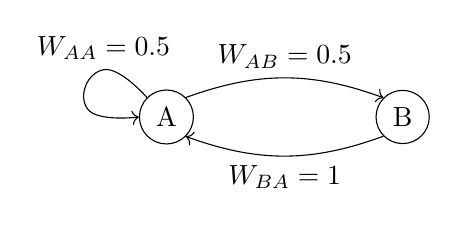
\begin{tikzpicture}
            \node[circle,draw] (A) at (0,0){A};
            \node[circle,draw] (B) at (3,0){B};
            \draw[->] (A.north east)to[bend left=20]node[above]{\(W_{AB}=0.5\)}(B.north west);
            \draw[->] (B.south west)to[bend left=20]node[below]{\(W_{BA}=1\)}(A.south east);
            \draw[->] plot[smooth, tension = 1] coordinates {(A.north west) (-0.8,0.6) (-1,0.1) (A.west) };
            \node at (-0.8,0.6)[above]{\(W_{AA}=0.5\)};
        \end{tikzpicture}
        \caption{An example of a Markov chain. At each time step, the system moves from one state to another with the given transition probability.}
    \end{figure}

    Suppose we have a stochastic process with a set of possible states \(S_1,S_2,S_3,\dots\) (finite, countably infinite or continuum) and discrete time \(t_1,t_2,\dots\). We denote the state of the system at time \(t_n\) as \(X_{t_n}\). Then for the process to be Markov, the conditional probability that the system will be in state \(X_{t_{n+1}}=S_j\) is only dependent on the current state of the system \(X_{t_n}=S_i\). It is independent of \(X_{t_{n-1}},X_{t_{n-2}},\dots\) or the value of \(n\). Hence, we can write the transition probability from state \(S_i\) to \(S_j\)
    \begin{equation}
        W_{ij}=W(S_i\to S_j)=\Prob(X_{t_{n+1}}=S_j\mid X_{t_n}=S_i)\,.
    \end{equation}
    As with usual probabilities, we require \(W_{ij}\ge 0\) and \(\sum_j W_{ij}=1\). Since \(\mathsf{W}\) can be considered as a matrix, it is also known as the \textit{transition matrix}.

    The total probability that at time \(t_n\) the system is in state \(S_j\) is
    \begin{equation}
        \Prob(X_{t_n}=S_j)=\sum_i W_{ij}\Prob(X_{t_{n-1}}=S_i)\,.
    \end{equation}
    If we treat time as continuous, \(\Prob(X_{t}=S_j)=P(S_j,t)\) and consider that the probability is conserved at all times: \(\sum_j P(S_j,t)=1\), then we get
    \begin{equation}
        \dv{P(S_j,t)}{t}=\sum_i[W_{ij}P(S_i,t)-W_{ji}P(S_j,t)]\,.
    \end{equation}
    The change in the probability of the system being in state \(S_j\) is the probability of moving into state \(S_j\) minus the probability of moving away from state \(j\).

    \subsubsection{Equilibrium and Detailed Balance}
    We say a system is in \textit{equilibrium} if the average macroscopic properties of the system have stopped changing, except for small fluctuations away from equilibrium that soon dissipate back towards equilibrium. The properties of a equilibrium system are independent of its history. Thus we can ignore how a system has reached equilibrium and focus on the distribution of microstates at equilibrium.

    Suppose the system is at equilibrium such that
    \begin{equation}
        \dv{P(S_j,t)}{t}=0\,,
    \end{equation}
    this means that
    \begin{equation}
        \sum_i[W_{ij}P_i^{\text{eq}}-W_{ji}P_j^{\text{eq}}]=0\,.
    \end{equation}
    The probability of moving out from \(S_j\) is equal to the probability of moving into \(S_j\). A sufficient but not necessary condition for this to happen is
    \begin{equation}
        W_{ij}P_i^{\text{eq}}=W_{ji}P_j^{\text{eq}}
    \end{equation}
    for all \(i,j\). This is known as the \textit{detailed balance}. In such case, the average number of moves from any state \(i\) to state \(j\) is equal to the number of moves from \(j\) to \(i\).

    In Metropolis Monte Carlo, we want the probability that the system sits in the microstate \(S_j\) is equal to its Boltzmann factor: \(P_j\propto \ee^{-\beta E_j}\). Then once the equilibrium has established, an ensemble of random walkers will populate the states \(S_j\) with the Boltzmann distribution that we desired. To achieve this, all we need to do is to choose the correct transition probabilities such that
    \begin{equation}
        \frac{W_{ij}}{W_{ji}}=\frac{P_j^{\text{eq}}}{P_i^{\text{eq}}}=\ee^{-\beta (E_j-E_i)}\,.
    \end{equation}

    The trick to determine the transition probability \(W_{ij}\) is to split it into two steps.
    \begin{enumerate}
        \item Choose a new configuration \(S_j\) with a selection probability \(\alpha_{ij}\).
        \item Accept or reject this new configuration with an acceptance probability \(P_{\text{acc}, ij}\). If accepted, move to \(S_j\), and if not, stay in \(S_i\).
    \end{enumerate}
    Then the transition probability can be written as
    \begin{equation}
        W_{ij}=\alpha_{ij}P_{\text{acc}, ij}\,.
    \end{equation}
    If we take \(\alpha\) to be symmetric, \(\alpha_{ij}=\alpha_{ji}\), then the condition of detailed balance becomes
    \begin{equation}
        \frac{P_{\text{acc}, ij}}{P_{\text{acc}, ji}}=\ee^{-\beta\Delta E}\,,
    \end{equation}
    where \(\Delta E=E_j-E_i\). There are many choices of \(P_{\text{acc}, ij}\) that satisfies this condition. The most popular choice is the \textit{algorithm of Metropolis}
    \begin{equation}
        P_{\text{acc}, ij}=\begin{cases}
            \ee^{-\beta \Delta E} & \text{if }\Delta E>0\\
            1 & \text{otherwise}
        \end{cases}\,.
    \end{equation}
    This means that if the energy decreases, you always accept the trial move, whereas if the energy increases, you accept it with a probability proportional to the Boltzmann factor of the energy difference. The clear advantage is now you don't need to evaluate the partition function.

    Note that for a Monte Carlo simulation to sample points in configurational space according to the correct Boltzmann weight, the detailed balance condition is sufficient but not necessary. There might exist correct sampling schemes that violate the detailed balance. However, unless we can prove that a non-detailed-balanced scheme yields the correct distribution, there is no point of doing so in practice.

    \begin{ex}
        \textit{Metropolis Monte Carlo for Interacting Fluid.}
        
        Consider an interacting fluid of \(N\) particles with positions \(\vb{r}^N=(\vb{r}_1,\vb{r}_2,\dots,\vb{r}_N)\) and momenta \(\vb{p}^N=(\vb{p}_1,\vb{p}_2,\dots,\vb{p}_N)\) interacting through the potential \(V(\vb{r}^N)\). When considering the energy \(E_i\) of a state \(i\), it includes both the kinetic energy and the potential energy, but as seen before, we can always integrate over the trivial momenta parts in the partition function to obtain
        \begin{equation}
            Q=\frac{1}{N!\Lambda^{3N}}Z_N\,.
        \end{equation}
        We can always ignore the momenta and do our MC averages over the states determined by \(\vb{r}^N\) alone, with the probability distribution
        \begin{equation}
            P(\vb{r}^N)=\frac{1}{Z_N}\exp[-\beta V(\vb{r}^N)]\,.
        \end{equation}

        To move from step \(k\) to step \(k+1\) in the Monte Carlo trajectory:
        \begin{enumerate}
            \item Select a fluid particle \(j\) at random from the configuration of step \(\vb{k}\):
            \begin{equation}
                \vb{r}_k^N=(\vb{r}_1,\vb{r}_2,\dots,\vb{r}_j,\dots,\vb{r}_N)\,.
            \end{equation}
            \item Move it to a new position with a random displacement \(\vb{r}_j'=\vb{r}_j+\vb{\Delta}\), with \(\Delta_i\in[-\delta,+\delta]\) for some \(\delta\).
            \item Calculate the potential energy \(V(\vb{r}_{\text{trial}}^{N})\) for the new state \(\vb{r}_{\text{trial}}^N=(\vb{r}_1,\dots,\vb{r}_j',\dots,\vb{r}_N)\).
            \item Accept the move \(\vb{r}_k^N\to\vb{r}_{\text{trial}}^N\) with a probability
            \begin{equation}
                P_{\text{acc}}(\vb{r}_k^N\to\vb{r}_{\text{trial}}^N)=\min\{1,\exp[-\beta(V(\vb{r}_{\text{trial}}^N)-V(\vb{r}_k^N))]\}\,.
            \end{equation}
            If the move is accepted, \(\vb{r}_{k+1}^N=\vb{r}_{\text{trial}}^N\). If not, \(\vb{r}_{k+1}^N=\vb{r}_k^N\).
        \end{enumerate}

        We need to have a suitable choice of our move step \(\vb{\Delta}\). If it is too large, most trial moves will be rejected, and if \(\vb{\Delta}\) is too small, you will move very slowly in the phase space, and it will take a large number of steps to reach equilibrium. For most systems, an average acceptance rate of \(20\%-30\%\) is suitable.

        In each MC step, we only attempt to move one particle, and so \(N\) separate MC steps are roughly equal to a single MD step, where all particles are moved together. Why don't we attempt to move \(N\) particles in a single MC step? There is no significant difference in computational cost between \(N\) single moves and one move of \(N\) particles in terms of evaluating \(V(\vb{r}_{\text{trial}}^N)\), but the rejection probability will be larger if we move all particles together. If the average probability of rejection for moving one atom is \(p_{\text{rej}}\), then the probability of an accepted move of \(N\) particles at once is \((1-p_{\text{rej}})^N\), which tends to zero as \(N\) increases. To get any acceptance at all in a collective move, we would require really small values of \(\vb{\Delta}\). Hence, for the same computational cost, single particle moves advance particles much faster than collective moves.
    \end{ex}

    \begin{ex}
        \textit{The Ising model}
        The Ising model has Hamiltonian
        \begin{equation}
            \mathcal{H}=-J\sum_{\eval{i,j}}S_iS_j-B\sum_i S_i\,,
        \end{equation}
        where \(S_i=\pm 1\) and \(\eval{i,j}\) denotes sum over all neighbouring pairs of particles. As you have investigated in Part II B7: \textit{Statistical Mechanics}, there are three competing effects. The neighbouring interactions want to keep everything aligned, the external field wants to keep everything to a specific direction, and the entropy wants to screw everything up as there are more disordered microstates than aligned microstates. At low temperatures, the ground state keeps (almost) all spins aligned with the external field, since then both the neighbouring alignment and the external field terms in the Hamiltonian will be simultaneously minimised. Defining the magnetisation
        \begin{equation}
            M=\frac{1}{N^2}\sum_i S_i\,,
        \end{equation}
        we can see that at low temperatures, \(M\to 1\) for \(B>0\) and \(M\to -1\) for \(B<0\).

        To do this in Monte Carlo, we can use the following scheme:
        \begin{enumerate}
            \item Start From an arbitrary initial configuration of spins.
            \item At step \(k\), select a random spin \(S_j(k)\) and flip it to \(-S_j(k)\).
            \item Evaluate the energy change
            \begin{equation}
                \Delta E=2S_j(k)\left[J\sum_{\text{neighbouring }n}S_n(k)+B\right]\,.
            \end{equation}
            \item Accept the move \(S_j(k)\to -S_j(k)\) with probability
            \begin{equation}
                P_{\text{acc}}(S_j(k)\to -S_j(k))=\min\{1,\exp(-\beta \Delta E)\}\,.
            \end{equation}
            If accepted, \(S_j(k+1)=-S_j(k)\), and if not, \(S_j(k+1)=S_j(k)\).
        \end{enumerate}

        \begin{figure}
            \centering
            % This file was created with tikzplotlib v0.10.1.
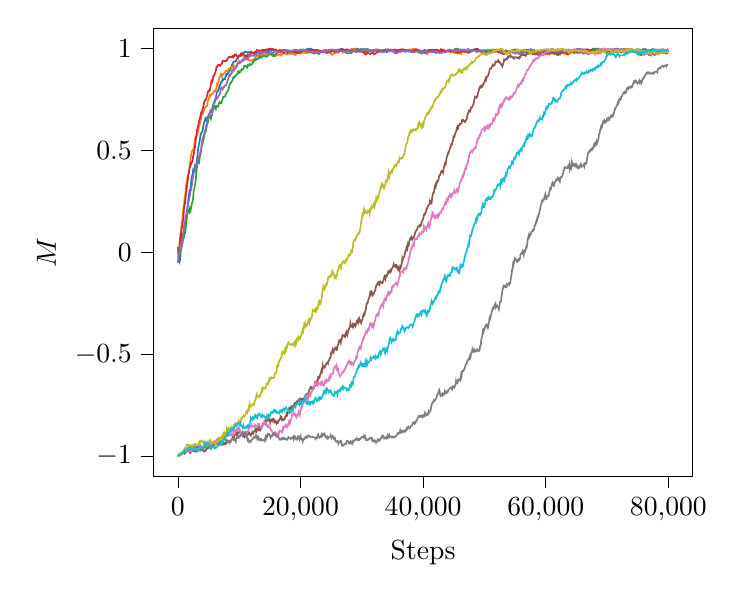
\begin{tikzpicture}

\definecolor{crimson2143940}{RGB}{214,39,40}
\definecolor{darkgray176}{RGB}{176,176,176}
\definecolor{darkorange25512714}{RGB}{255,127,14}
\definecolor{darkturquoise23190207}{RGB}{23,190,207}
\definecolor{forestgreen4416044}{RGB}{44,160,44}
\definecolor{goldenrod18818934}{RGB}{188,189,34}
\definecolor{gray127}{RGB}{127,127,127}
\definecolor{mediumpurple148103189}{RGB}{148,103,189}
\definecolor{orchid227119194}{RGB}{227,119,194}
\definecolor{sienna1408675}{RGB}{140,86,75}
\definecolor{steelblue31119180}{RGB}{31,119,180}

\begin{axis}[
tick align=outside,
tick pos=left,
x grid style={darkgray176},
xlabel={Steps},
xmin=-4000, xmax=84000,
xtick style={color=black},
ylabel={\(M\)},
scaled ticks=false,
y grid style={darkgray176},
ymin=-1.1, ymax=1.1,
ytick style={color=black}
]
\addplot [semithick, steelblue31119180]
table {%
0 -0.0489
100 -0.0378
200 -0.0289
300 -0.0444
400 -0.0333
500 0.0156
600 0.0244
700 0.0356
800 0.0511
900 0.0711
1000 0.0778
1100 0.1022
1200 0.1044
1300 0.1467
1400 0.1756
1500 0.1978
1600 0.2222
1700 0.2533
1800 0.2778
1900 0.3022
2000 0.3044
2100 0.3222
2200 0.3533
2300 0.3711
2400 0.3844
2500 0.4022
2600 0.3911
2700 0.3956
2800 0.4222
2900 0.4156
3000 0.4289
3100 0.4467
3200 0.4756
3300 0.5044
3400 0.5244
3500 0.5378
3600 0.5533
3700 0.5733
3800 0.5844
3900 0.5889
4000 0.5933
4100 0.6089
4200 0.6267
4300 0.64
4400 0.6444
4500 0.6578
4600 0.6533
4700 0.6467
4800 0.6622
4900 0.6667
5000 0.6689
5100 0.6778
5200 0.6844
5300 0.6867
5400 0.6867
5500 0.6889
5600 0.6933
5700 0.7178
5800 0.7289
5900 0.7311
6000 0.7489
6100 0.7511
6200 0.7556
6300 0.7756
6400 0.7867
6500 0.7889
6600 0.8
6700 0.8022
6800 0.8178
6900 0.8222
7000 0.8289
7100 0.8378
7200 0.8378
7300 0.8511
7400 0.8467
7500 0.8489
7600 0.8511
7700 0.8511
7800 0.8689
7900 0.8667
8000 0.8756
8100 0.8756
8200 0.88
8300 0.8844
8400 0.8889
8500 0.8933
8600 0.8956
8700 0.9067
8800 0.92
8900 0.92
9000 0.9311
9100 0.9356
9200 0.9356
9300 0.9356
9400 0.94
9500 0.94
9600 0.9467
9700 0.9511
9800 0.9511
9900 0.96
10000 0.9644
10100 0.9644
10200 0.9644
10300 0.9667
10400 0.9644
10500 0.9711
10600 0.9756
10700 0.9733
10800 0.98
10900 0.9844
11000 0.9822
11100 0.9844
11200 0.9844
11300 0.9822
11400 0.98
11500 0.9822
11600 0.9822
11700 0.9822
11800 0.9822
11900 0.9844
12000 0.9844
12100 0.98
12200 0.9778
12300 0.9778
12400 0.9778
12500 0.98
12600 0.9778
12700 0.9822
12800 0.98
12900 0.9822
13000 0.9822
13100 0.9822
13200 0.9822
13300 0.9822
13400 0.9778
13500 0.98
13600 0.9822
13700 0.98
13800 0.98
13900 0.9844
14000 0.9867
14100 0.9867
14200 0.9844
14300 0.9867
14400 0.9867
14500 0.9867
14600 0.9867
14700 0.9889
14800 0.9867
14900 0.9889
15000 0.9933
15100 0.9933
15200 0.9911
15300 0.9933
15400 0.9933
15500 0.9911
15600 0.9911
15700 0.9889
15800 0.9867
15900 0.9867
16000 0.9867
16100 0.9889
16200 0.9889
16300 0.9889
16400 0.9889
16500 0.9889
16600 0.9889
16700 0.9889
16800 0.9889
16900 0.9867
17000 0.9867
17100 0.9867
17200 0.9867
17300 0.9867
17400 0.9889
17500 0.9867
17600 0.9844
17700 0.9867
17800 0.9867
17900 0.9867
18000 0.9844
18100 0.98
18200 0.9844
18300 0.9844
18400 0.9844
18500 0.9844
18600 0.9844
18700 0.9867
18800 0.9867
18900 0.9867
19000 0.9889
19100 0.9889
19200 0.9867
19300 0.9867
19400 0.9889
19500 0.9911
19600 0.9911
19700 0.9911
19800 0.9889
19900 0.9911
20000 0.9933
20100 0.9956
20200 0.9933
20300 0.9911
20400 0.9889
20500 0.9889
20600 0.9867
20700 0.9889
20800 0.9911
20900 0.9933
21000 0.9956
21100 0.9956
21200 0.9978
21300 0.9956
21400 0.9978
21500 0.9978
21600 1
21700 0.9978
21800 0.9978
21900 0.9956
22000 0.9956
22100 0.9933
22200 0.9933
22300 0.9911
22400 0.9911
22500 0.9889
22600 0.9867
22700 0.9822
22800 0.9844
22900 0.9844
23000 0.9844
23100 0.9844
23200 0.9844
23300 0.9867
23400 0.9844
23500 0.9889
23600 0.9889
23700 0.9889
23800 0.9889
23900 0.9889
24000 0.9889
24100 0.9933
24200 0.9933
24300 0.9911
24400 0.9911
24500 0.9911
24600 0.9933
24700 0.9933
24800 0.9889
24900 0.9911
25000 0.9911
25100 0.9911
25200 0.9911
25300 0.9933
25400 0.9933
25500 0.9933
25600 0.9933
25700 0.9933
25800 0.9933
25900 0.9933
26000 0.9956
26100 0.9933
26200 0.9956
26300 0.9956
26400 0.9956
26500 0.9933
26600 0.9978
26700 0.9978
26800 0.9956
26900 0.9956
27000 0.9933
27100 0.9911
27200 0.9933
27300 0.9933
27400 0.9933
27500 0.9933
27600 0.9933
27700 0.9933
27800 0.9933
27900 0.9933
28000 0.9911
28100 0.9911
28200 0.9956
28300 0.9956
28400 0.9956
28500 0.9956
28600 0.9978
28700 0.9978
28800 0.9978
28900 0.9978
29000 1
29100 1
29200 1
29300 1
29400 0.9978
29500 0.9956
29600 0.9956
29700 0.9956
29800 0.9956
29900 0.9956
30000 0.9956
30100 0.9956
30200 0.9956
30300 0.9956
30400 0.9978
30500 0.9956
30600 0.9956
30700 0.9956
30800 0.9933
30900 0.9911
31000 0.9911
31100 0.9911
31200 0.9933
31300 0.9911
31400 0.9933
31500 0.9911
31600 0.9911
31700 0.9911
31800 0.9911
31900 0.9889
32000 0.9933
32100 0.9933
32200 0.9911
32300 0.9911
32400 0.9911
32500 0.9867
32600 0.9889
32700 0.9889
32800 0.9911
32900 0.9867
33000 0.9867
33100 0.9867
33200 0.9889
33300 0.9889
33400 0.9911
33500 0.9911
33600 0.9911
33700 0.9911
33800 0.9911
33900 0.9867
34000 0.9844
34100 0.9822
34200 0.9844
34300 0.9867
34400 0.9867
34500 0.9933
34600 0.9911
34700 0.9911
34800 0.9933
34900 0.9911
35000 0.9889
35100 0.9911
35200 0.9933
35300 0.9933
35400 0.9956
35500 0.9933
35600 0.9889
35700 0.9889
35800 0.9867
35900 0.9867
36000 0.9889
36100 0.9911
36200 0.9911
36300 0.9911
36400 0.9889
36500 0.9911
36600 0.9911
36700 0.9911
36800 0.9911
36900 0.9889
37000 0.9911
37100 0.9911
37200 0.9889
37300 0.9867
37400 0.9889
37500 0.9889
37600 0.9867
37700 0.9933
37800 0.9933
37900 0.9911
38000 0.9889
38100 0.9889
38200 0.9889
38300 0.9889
38400 0.9911
38500 0.9889
38600 0.9867
38700 0.9911
38800 0.9867
38900 0.9889
39000 0.9911
39100 0.9889
39200 0.9867
39300 0.9844
39400 0.9844
39500 0.9844
39600 0.9844
39700 0.9844
39800 0.9844
39900 0.9867
40000 0.9867
40100 0.9867
40200 0.9933
40300 0.9933
40400 0.9911
40500 0.9911
40600 0.9889
40700 0.9889
40800 0.9911
40900 0.9933
41000 0.9933
41100 0.9933
41200 0.9933
41300 0.9933
41400 0.9933
41500 0.9933
41600 0.9911
41700 0.9911
41800 0.9889
41900 0.9889
42000 0.9889
42100 0.9889
42200 0.9867
42300 0.9822
42400 0.9822
42500 0.9822
42600 0.98
42700 0.98
42800 0.9867
42900 0.9867
43000 0.9911
43100 0.9911
43200 0.9911
43300 0.9933
43400 0.9911
43500 0.9911
43600 0.9867
43700 0.9889
43800 0.9867
43900 0.9889
44000 0.9867
44100 0.9889
44200 0.9911
44300 0.9889
44400 0.9844
44500 0.9867
44600 0.9867
44700 0.9844
44800 0.9844
44900 0.9889
45000 0.9867
45100 0.9867
45200 0.9889
45300 0.9822
45400 0.9867
45500 0.9867
45600 0.9889
45700 0.9889
45800 0.9933
45900 0.9933
46000 0.9911
46100 0.9911
46200 0.9911
46300 0.9933
46400 0.9933
46500 0.9911
46600 0.9911
46700 0.9889
46800 0.9889
46900 0.9867
47000 0.9889
47100 0.9911
47200 0.9933
47300 0.9978
47400 0.9956
47500 0.9956
47600 0.9933
47700 0.9911
47800 0.9911
47900 0.9889
48000 0.9889
48100 0.9911
48200 0.9911
48300 0.9933
48400 0.9933
48500 0.9978
48600 0.9956
48700 0.9956
48800 0.9956
48900 0.9978
49000 0.9933
49100 0.9911
49200 0.9889
49300 0.9911
49400 0.9911
49500 0.9911
49600 0.9889
49700 0.9867
49800 0.9844
49900 0.9911
50000 0.9889
50100 0.9889
50200 0.9844
50300 0.9822
50400 0.9822
50500 0.9844
50600 0.98
50700 0.98
50800 0.9822
50900 0.9822
51000 0.9844
51100 0.9822
51200 0.9867
51300 0.9867
51400 0.9889
51500 0.9867
51600 0.9889
51700 0.9889
51800 0.9889
51900 0.9889
52000 0.9889
52100 0.9889
52200 0.9889
52300 0.9822
52400 0.9844
52500 0.9844
52600 0.9844
52700 0.9844
52800 0.9822
52900 0.9822
53000 0.9867
53100 0.9844
53200 0.9867
53300 0.9844
53400 0.9867
53500 0.9911
53600 0.9867
53700 0.9867
53800 0.9867
53900 0.9867
54000 0.9889
54100 0.9844
54200 0.9867
54300 0.9867
54400 0.9889
54500 0.9889
54600 0.9933
54700 0.9933
54800 0.9911
54900 0.9933
55000 0.9889
55100 0.9867
55200 0.9889
55300 0.9889
55400 0.9889
55500 0.9867
55600 0.9889
55700 0.9889
55800 0.9867
55900 0.9867
56000 0.9844
56100 0.9867
56200 0.9867
56300 0.9867
56400 0.9911
56500 0.9889
56600 0.9889
56700 0.9911
56800 0.9911
56900 0.9933
57000 0.9889
57100 0.9911
57200 0.9933
57300 0.9911
57400 0.9911
57500 0.9956
57600 0.9911
57700 0.9889
57800 0.9867
57900 0.9867
58000 0.9867
58100 0.9844
58200 0.9867
58300 0.9867
58400 0.9844
58500 0.9844
58600 0.9867
58700 0.9844
58800 0.9867
58900 0.9867
59000 0.9867
59100 0.9911
59200 0.9867
59300 0.9867
59400 0.9822
59500 0.9822
59600 0.9822
59700 0.9822
59800 0.9822
59900 0.9867
60000 0.9867
60100 0.9867
60200 0.9911
60300 0.9911
60400 0.9889
60500 0.9911
60600 0.9911
60700 0.9889
60800 0.9889
60900 0.9956
61000 0.9978
61100 0.9978
61200 0.9956
61300 0.9933
61400 0.9933
61500 0.9911
61600 0.9933
61700 0.9933
61800 0.9933
61900 0.9889
62000 0.9889
62100 0.9889
62200 0.9889
62300 0.9911
62400 0.9911
62500 0.9911
62600 0.9911
62700 0.9933
62800 0.9933
62900 0.9933
63000 0.9911
63100 0.9911
63200 0.9911
63300 0.9889
63400 0.9867
63500 0.9844
63600 0.9844
63700 0.9844
63800 0.9867
63900 0.9889
64000 0.9867
64100 0.9867
64200 0.9867
64300 0.9889
64400 0.9889
64500 0.9822
64600 0.9822
64700 0.9778
64800 0.9822
64900 0.9867
65000 0.9889
65100 0.9889
65200 0.9867
65300 0.9867
65400 0.9867
65500 0.9867
65600 0.9867
65700 0.9889
65800 0.9889
65900 0.9889
66000 0.9889
66100 0.9889
66200 0.9867
66300 0.9867
66400 0.9844
66500 0.9844
66600 0.9822
66700 0.9867
66800 0.9844
66900 0.9844
67000 0.9822
67100 0.9778
67200 0.98
67300 0.9844
67400 0.9889
67500 0.9933
67600 0.9933
67700 0.9978
67800 1
67900 0.9978
68000 0.9978
68100 0.9933
68200 0.9933
68300 0.9889
68400 0.9889
68500 0.9911
68600 0.9911
68700 0.9911
68800 0.9911
68900 0.9933
69000 0.9911
69100 0.9911
69200 0.9911
69300 0.9889
69400 0.9889
69500 0.9911
69600 0.9867
69700 0.9844
69800 0.9844
69900 0.9778
70000 0.9822
70100 0.9844
70200 0.9889
70300 0.9911
70400 0.9911
70500 0.9911
70600 0.9933
70700 0.9933
70800 0.9933
70900 0.9911
71000 0.9889
71100 0.9889
71200 0.9911
71300 0.9933
71400 0.9933
71500 0.9889
71600 0.9889
71700 0.9911
71800 0.9911
71900 0.9911
72000 0.9911
72100 0.9933
72200 0.9911
72300 0.9911
72400 0.9889
72500 0.9889
72600 0.9889
72700 0.9911
72800 0.9867
72900 0.9844
73000 0.9844
73100 0.9822
73200 0.9822
73300 0.9844
73400 0.9889
73500 0.9933
73600 0.9933
73700 0.9933
73800 0.9956
73900 0.9956
74000 0.9933
74100 0.9911
74200 0.9911
74300 0.9889
74400 0.9889
74500 0.9867
74600 0.9867
74700 0.9867
74800 0.9867
74900 0.9889
75000 0.9978
75100 0.9956
75200 0.9956
75300 0.9956
75400 0.9933
75500 0.9911
75600 0.9911
75700 0.9911
75800 0.9956
75900 0.9978
76000 0.9956
76100 0.9956
76200 0.9978
76300 0.9956
76400 0.9956
76500 0.9933
76600 0.9911
76700 0.9867
76800 0.9867
76900 0.9822
77000 0.9844
77100 0.9822
77200 0.9844
77300 0.9911
77400 0.9911
77500 0.9911
77600 0.9933
77700 0.9933
77800 0.9933
77900 0.9911
78000 0.9867
78100 0.9844
78200 0.9844
78300 0.9822
78400 0.9844
78500 0.9844
78600 0.9844
78700 0.9867
78800 0.9867
78900 0.9822
79000 0.98
79100 0.9778
79200 0.9778
79300 0.98
79400 0.9822
79500 0.9778
79600 0.9756
79700 0.9778
79800 0.9778
79900 0.98
80000 0.98
};
\addplot [semithick, darkorange25512714]
table {%
0 0.0222
100 0.0089
200 0.02
300 0.0489
400 0.0911
500 0.0911
600 0.1289
700 0.1511
800 0.1822
900 0.2133
1000 0.2289
1100 0.2667
1200 0.28
1300 0.3133
1400 0.3356
1500 0.3533
1600 0.3756
1700 0.38
1800 0.3933
1900 0.4178
2000 0.4378
2100 0.4667
2200 0.4822
2300 0.4956
2400 0.5
2500 0.5022
2600 0.5133
2700 0.5311
2800 0.5578
2900 0.5667
3000 0.5667
3100 0.5733
3200 0.5822
3300 0.5867
3400 0.6133
3500 0.62
3600 0.6289
3700 0.6422
3800 0.6578
3900 0.6778
4000 0.6778
4100 0.68
4200 0.6911
4300 0.6978
4400 0.7089
4500 0.7111
4600 0.7156
4700 0.7178
4800 0.72
4900 0.7422
5000 0.7489
5100 0.76
5200 0.7711
5300 0.7667
5400 0.7733
5500 0.7733
5600 0.78
5700 0.78
5800 0.7822
5900 0.7911
6000 0.7933
6100 0.7911
6200 0.7978
6300 0.8067
6400 0.8267
6500 0.8244
6600 0.8356
6700 0.8489
6800 0.8578
6900 0.8622
7000 0.8733
7100 0.8667
7200 0.8733
7300 0.8689
7400 0.8733
7500 0.8778
7600 0.88
7700 0.8822
7800 0.8911
7900 0.8911
8000 0.8889
8100 0.8911
8200 0.8956
8300 0.9
8400 0.9022
8500 0.9044
8600 0.9067
8700 0.9089
8800 0.9044
8900 0.9089
9000 0.9133
9100 0.92
9200 0.9133
9300 0.9133
9400 0.9089
9500 0.9111
9600 0.9156
9700 0.9222
9800 0.9311
9900 0.9378
10000 0.94
10100 0.9356
10200 0.9333
10300 0.9333
10400 0.9356
10500 0.9378
10600 0.9444
10700 0.9511
10800 0.9578
10900 0.9533
11000 0.9556
11100 0.9533
11200 0.9511
11300 0.9578
11400 0.9533
11500 0.9489
11600 0.9422
11700 0.9422
11800 0.9422
11900 0.94
12000 0.94
12100 0.9378
12200 0.9444
12300 0.9467
12400 0.9467
12500 0.9489
12600 0.9533
12700 0.9578
12800 0.96
12900 0.9622
13000 0.9622
13100 0.9667
13200 0.9644
13300 0.9644
13400 0.9667
13500 0.9644
13600 0.9711
13700 0.9711
13800 0.9711
13900 0.9667
14000 0.9711
14100 0.9711
14200 0.9711
14300 0.9778
14400 0.9778
14500 0.98
14600 0.9778
14700 0.9778
14800 0.9778
14900 0.9822
15000 0.9844
15100 0.9844
15200 0.9822
15300 0.98
15400 0.9733
15500 0.9711
15600 0.9733
15700 0.9711
15800 0.9667
15900 0.9622
16000 0.9644
16100 0.9689
16200 0.9667
16300 0.9667
16400 0.9689
16500 0.9711
16600 0.9711
16700 0.9689
16800 0.9667
16900 0.9711
17000 0.9711
17100 0.9756
17200 0.9756
17300 0.9756
17400 0.9756
17500 0.9756
17600 0.9756
17700 0.9756
17800 0.9711
17900 0.9711
18000 0.9756
18100 0.9756
18200 0.9778
18300 0.9733
18400 0.9756
18500 0.9756
18600 0.9756
18700 0.9778
18800 0.9733
18900 0.9733
19000 0.9711
19100 0.9733
19200 0.9689
19300 0.9733
19400 0.9778
19500 0.9778
19600 0.9822
19700 0.9844
19800 0.9822
19900 0.9778
20000 0.9756
20100 0.98
20200 0.9778
20300 0.9822
20400 0.98
20500 0.98
20600 0.98
20700 0.9822
20800 0.9778
20900 0.9778
21000 0.98
21100 0.98
21200 0.9778
21300 0.9822
21400 0.98
21500 0.9822
21600 0.9822
21700 0.9822
21800 0.9844
21900 0.9822
22000 0.9822
22100 0.9822
22200 0.9844
22300 0.9844
22400 0.9844
22500 0.9867
22600 0.9889
22700 0.9889
22800 0.9911
22900 0.9867
23000 0.9844
23100 0.9867
23200 0.9844
23300 0.9867
23400 0.9889
23500 0.9911
23600 0.9911
23700 0.9911
23800 0.9889
23900 0.9911
24000 0.9911
24100 0.9911
24200 0.9911
24300 0.9889
24400 0.9844
24500 0.9844
24600 0.9867
24700 0.9844
24800 0.98
24900 0.9756
25000 0.9733
25100 0.9711
25200 0.9689
25300 0.9711
25400 0.9756
25500 0.9756
25600 0.9778
25700 0.9867
25800 0.9867
25900 0.98
26000 0.98
26100 0.98
26200 0.9822
26300 0.9844
26400 0.9867
26500 0.9867
26600 0.9889
26700 0.9889
26800 0.9889
26900 0.9822
27000 0.9867
27100 0.9889
27200 0.9889
27300 0.9889
27400 0.9911
27500 0.9911
27600 0.9911
27700 0.9911
27800 0.9933
27900 0.9933
28000 0.9933
28100 0.9933
28200 0.9956
28300 0.9978
28400 0.9978
28500 0.9978
28600 0.9978
28700 0.9978
28800 0.9933
28900 0.9956
29000 0.9933
29100 0.9933
29200 0.9933
29300 0.9933
29400 0.9933
29500 0.9956
29600 0.9956
29700 0.9956
29800 0.9933
29900 0.9933
30000 0.9933
30100 0.9956
30200 0.9956
30300 0.9933
30400 0.9933
30500 0.9911
30600 0.9889
30700 0.9867
30800 0.9867
30900 0.9844
31000 0.9867
31100 0.9889
31200 0.9889
31300 0.9911
31400 0.9911
31500 0.9933
31600 0.9933
31700 0.9933
31800 0.9933
31900 0.9933
32000 0.9911
32100 0.9933
32200 0.9933
32300 0.9911
32400 0.9933
32500 0.9911
32600 0.9889
32700 0.9889
32800 0.9867
32900 0.9889
33000 0.9889
33100 0.9889
33200 0.9889
33300 0.9889
33400 0.9933
33500 0.9911
33600 0.9933
33700 0.9933
33800 0.9933
33900 0.9911
34000 0.9911
34100 0.9911
34200 0.9956
34300 0.9956
34400 0.9933
34500 0.9889
34600 0.9867
34700 0.9867
34800 0.9867
34900 0.9867
35000 0.9889
35100 0.9844
35200 0.9822
35300 0.9822
35400 0.9778
35500 0.9778
35600 0.9822
35700 0.98
35800 0.9822
35900 0.9867
36000 0.9844
36100 0.9889
36200 0.9889
36300 0.9889
36400 0.9867
36500 0.9867
36600 0.9889
36700 0.9911
36800 0.9911
36900 0.9911
37000 0.9911
37100 0.9911
37200 0.9933
37300 0.9933
37400 0.9911
37500 0.9911
37600 0.9889
37700 0.9911
37800 0.9956
37900 0.9933
38000 0.9956
38100 0.9956
38200 0.9956
38300 0.9978
38400 0.9978
38500 0.9978
38600 0.9978
38700 0.9978
38800 0.9978
38900 0.9956
39000 0.9956
39100 0.9911
39200 0.9911
39300 0.9933
39400 0.9911
39500 0.9911
39600 0.9889
39700 0.9867
39800 0.9822
39900 0.9822
40000 0.9844
40100 0.9822
40200 0.98
40300 0.98
40400 0.9778
40500 0.98
40600 0.9778
40700 0.9733
40800 0.98
40900 0.9822
41000 0.9844
41100 0.9844
41200 0.9867
41300 0.9867
41400 0.9867
41500 0.9889
41600 0.9867
41700 0.9867
41800 0.9889
41900 0.9867
42000 0.9889
42100 0.9911
42200 0.9911
42300 0.9933
42400 0.9933
42500 0.9933
42600 0.9911
42700 0.9889
42800 0.9933
42900 0.9933
43000 0.9933
43100 0.9911
43200 0.9889
43300 0.9889
43400 0.9889
43500 0.9889
43600 0.9889
43700 0.9889
43800 0.9889
43900 0.9889
44000 0.9867
44100 0.9867
44200 0.9889
44300 0.9867
44400 0.9844
44500 0.9822
44600 0.9844
44700 0.9822
44800 0.9822
44900 0.9822
45000 0.98
45100 0.9822
45200 0.9822
45300 0.9844
45400 0.9844
45500 0.9778
45600 0.9756
45700 0.9756
45800 0.9756
45900 0.9756
46000 0.9778
46100 0.9756
46200 0.9733
46300 0.98
46400 0.9844
46500 0.9867
46600 0.9867
46700 0.9911
46800 0.9911
46900 0.9911
47000 0.9911
47100 0.9911
47200 0.9933
47300 0.9933
47400 0.9933
47500 0.9933
47600 0.9889
47700 0.9889
47800 0.9867
47900 0.9889
48000 0.9911
48100 0.9933
48200 0.9933
48300 0.9933
48400 0.9933
48500 0.9911
48600 0.9911
48700 0.9889
48800 0.9867
48900 0.9844
49000 0.9844
49100 0.9867
49200 0.9911
49300 0.9911
49400 0.9911
49500 0.9889
49600 0.9911
49700 0.9911
49800 0.9933
49900 0.9911
50000 0.9911
50100 0.9911
50200 0.9911
50300 0.9933
50400 0.9933
50500 0.9933
50600 0.9933
50700 0.9933
50800 0.9956
50900 0.9933
51000 0.9933
51100 0.9933
51200 0.9933
51300 0.9956
51400 0.9956
51500 0.9956
51600 0.9933
51700 0.9933
51800 0.9933
51900 0.9933
52000 0.9956
52100 0.9933
52200 0.9933
52300 0.9933
52400 0.9911
52500 0.9933
52600 0.9933
52700 0.9911
52800 0.9867
52900 0.9844
53000 0.9844
53100 0.9844
53200 0.9844
53300 0.9822
53400 0.9867
53500 0.9867
53600 0.9867
53700 0.9844
53800 0.9867
53900 0.9867
54000 0.9844
54100 0.9844
54200 0.9844
54300 0.9889
54400 0.9889
54500 0.9844
54600 0.9911
54700 0.9867
54800 0.9889
54900 0.9933
55000 0.9933
55100 0.9889
55200 0.9911
55300 0.9889
55400 0.9867
55500 0.9844
55600 0.9844
55700 0.9867
55800 0.9911
55900 0.9889
56000 0.9911
56100 0.9911
56200 0.9911
56300 0.9933
56400 0.9911
56500 0.9911
56600 0.9933
56700 0.9933
56800 0.9911
56900 0.9867
57000 0.9889
57100 0.9911
57200 0.9911
57300 0.9889
57400 0.9889
57500 0.9867
57600 0.9844
57700 0.9867
57800 0.9867
57900 0.9844
58000 0.9822
58100 0.9822
58200 0.9778
58300 0.98
58400 0.98
58500 0.9778
58600 0.9756
58700 0.9756
58800 0.98
58900 0.98
59000 0.9756
59100 0.9733
59200 0.9778
59300 0.9756
59400 0.9778
59500 0.9711
59600 0.9733
59700 0.9756
59800 0.9822
59900 0.9778
60000 0.9778
60100 0.9778
60200 0.98
60300 0.9756
60400 0.9733
60500 0.9711
60600 0.9711
60700 0.9778
60800 0.98
60900 0.98
61000 0.9756
61100 0.9778
61200 0.98
61300 0.9822
61400 0.9844
61500 0.9867
61600 0.9867
61700 0.9844
61800 0.9867
61900 0.9889
62000 0.9911
62100 0.9844
62200 0.9822
62300 0.9867
62400 0.9844
62500 0.9867
62600 0.9844
62700 0.98
62800 0.98
62900 0.98
63000 0.98
63100 0.9733
63200 0.9756
63300 0.9756
63400 0.9733
63500 0.9756
63600 0.9822
63700 0.9822
63800 0.9822
63900 0.9844
64000 0.9822
64100 0.9844
64200 0.9822
64300 0.9844
64400 0.9844
64500 0.98
64600 0.98
64700 0.9844
64800 0.9822
64900 0.9844
65000 0.9867
65100 0.9867
65200 0.9867
65300 0.9867
65400 0.9867
65500 0.9844
65600 0.9844
65700 0.9889
65800 0.9822
65900 0.9867
66000 0.9867
66100 0.9889
66200 0.9889
66300 0.9933
66400 0.9933
66500 0.9933
66600 0.9933
66700 0.9956
66800 0.9911
66900 0.9911
67000 0.9889
67100 0.9867
67200 0.9867
67300 0.9844
67400 0.9867
67500 0.9889
67600 0.9867
67700 0.9889
67800 0.9889
67900 0.9867
68000 0.9889
68100 0.9889
68200 0.9911
68300 0.9867
68400 0.9911
68500 0.9933
68600 0.9933
68700 0.9911
68800 0.9933
68900 0.9933
69000 0.9956
69100 0.9978
69200 0.9978
69300 0.9978
69400 0.9978
69500 0.9978
69600 1
69700 0.9978
69800 0.9956
69900 0.9956
70000 0.9956
70100 0.9956
70200 0.9911
70300 0.9911
70400 0.9933
70500 0.9911
70600 0.9933
70700 0.9911
70800 0.9911
70900 0.9867
71000 0.9911
71100 0.9956
71200 0.9956
71300 0.9956
71400 0.9978
71500 0.9933
71600 0.9911
71700 0.9911
71800 0.9911
71900 0.9933
72000 0.9933
72100 0.9933
72200 0.9956
72300 0.9911
72400 0.9933
72500 0.9933
72600 0.9956
72700 0.9978
72800 0.9978
72900 0.9978
73000 0.9978
73100 0.9978
73200 0.9978
73300 0.9978
73400 0.9978
73500 0.9956
73600 0.9956
73700 0.9933
73800 0.9911
73900 0.9889
74000 0.9889
74100 0.9911
74200 0.9911
74300 0.9911
74400 0.9889
74500 0.9889
74600 0.9889
74700 0.9889
74800 0.9867
74900 0.9889
75000 0.9867
75100 0.9889
75200 0.9911
75300 0.9911
75400 0.9889
75500 0.9889
75600 0.9867
75700 0.9889
75800 0.9889
75900 0.9889
76000 0.9889
76100 0.9933
76200 0.9889
76300 0.9911
76400 0.9911
76500 0.9933
76600 0.9933
76700 0.9933
76800 0.9911
76900 0.9911
77000 0.9933
77100 0.9933
77200 0.9911
77300 0.9933
77400 0.9911
77500 0.9911
77600 0.9933
77700 0.9933
77800 0.9933
77900 0.9956
78000 0.9956
78100 0.9933
78200 0.9911
78300 0.9889
78400 0.9889
78500 0.9867
78600 0.9911
78700 0.9933
78800 0.9933
78900 0.9933
79000 0.9889
79100 0.9911
79200 0.9889
79300 0.9889
79400 0.9867
79500 0.9844
79600 0.9844
79700 0.9844
79800 0.9867
79900 0.9867
80000 0.9867
};
\addplot [semithick, forestgreen4416044]
table {%
0 0.0267
100 -0.02
200 -0.0178
300 -0.0111
400 0.0044
500 0.0222
600 0.0333
700 0.0689
800 0.0889
900 0.0911
1000 0.08
1100 0.0933
1200 0.0933
1300 0.1267
1400 0.1511
1500 0.1756
1600 0.1933
1700 0.2044
1800 0.2089
1900 0.2
2000 0.2156
2100 0.2067
2200 0.2244
2300 0.24
2400 0.2489
2500 0.2667
2600 0.3044
2700 0.3133
2800 0.3333
2900 0.3467
3000 0.3822
3100 0.4111
3200 0.4333
3300 0.4467
3400 0.4556
3500 0.4467
3600 0.4689
3700 0.4778
3800 0.5
3900 0.5222
4000 0.5267
4100 0.5422
4200 0.5533
4300 0.5667
4400 0.5867
4500 0.5978
4600 0.5956
4700 0.6156
4800 0.6333
4900 0.6378
5000 0.6533
5100 0.6622
5200 0.6644
5300 0.6689
5400 0.6578
5500 0.6711
5600 0.6756
5700 0.6933
5800 0.7044
5900 0.7067
6000 0.7178
6100 0.7178
6200 0.7067
6300 0.72
6400 0.72
6500 0.7178
6600 0.7156
6700 0.7311
6800 0.7378
6900 0.7333
7000 0.7333
7100 0.7333
7200 0.7422
7300 0.7511
7400 0.7622
7500 0.7622
7600 0.7644
7700 0.7644
7800 0.7756
7900 0.78
8000 0.7867
8100 0.7911
8200 0.7956
8300 0.8044
8400 0.8178
8500 0.8267
8600 0.8311
8700 0.8333
8800 0.84
8900 0.8422
9000 0.8556
9100 0.86
9200 0.8578
9300 0.8622
9400 0.8667
9500 0.8689
9600 0.8711
9700 0.8756
9800 0.8867
9900 0.8889
10000 0.8822
10100 0.8867
10200 0.8867
10300 0.8911
10400 0.8978
10500 0.8956
10600 0.8978
10700 0.9
10800 0.9133
10900 0.9156
11000 0.9133
11100 0.9133
11200 0.9111
11300 0.9067
11400 0.9178
11500 0.9156
11600 0.9178
11700 0.9244
11800 0.9222
11900 0.92
12000 0.9222
12100 0.9244
12200 0.9289
12300 0.9333
12400 0.9378
12500 0.9467
12600 0.9467
12700 0.9444
12800 0.9489
12900 0.9467
13000 0.9489
13100 0.9511
13200 0.9511
13300 0.9622
13400 0.9578
13500 0.9556
13600 0.9556
13700 0.9578
13800 0.9622
13900 0.9644
14000 0.9644
14100 0.9622
14200 0.9622
14300 0.9644
14400 0.9622
14500 0.96
14600 0.9622
14700 0.9667
14800 0.9689
14900 0.9733
15000 0.9756
15100 0.9711
15200 0.9733
15300 0.9711
15400 0.9667
15500 0.9644
15600 0.9667
15700 0.9644
15800 0.9711
15900 0.9711
16000 0.9733
16100 0.9778
16200 0.98
16300 0.98
16400 0.9889
16500 0.9889
16600 0.9889
16700 0.9911
16800 0.9889
16900 0.9889
17000 0.9911
17100 0.9933
17200 0.9911
17300 0.9933
17400 0.9933
17500 0.9933
17600 0.9911
17700 0.9911
17800 0.9933
17900 0.9911
18000 0.9911
18100 0.9911
18200 0.9911
18300 0.9867
18400 0.9844
18500 0.9822
18600 0.9844
18700 0.9844
18800 0.9867
18900 0.9889
19000 0.9889
19100 0.9889
19200 0.9889
19300 0.9867
19400 0.9822
19500 0.98
19600 0.9778
19700 0.9778
19800 0.9778
19900 0.9822
20000 0.9844
20100 0.9844
20200 0.9911
20300 0.9933
20400 0.9933
20500 0.9933
20600 0.9911
20700 0.9933
20800 0.9889
20900 0.9867
21000 0.9889
21100 0.9867
21200 0.9867
21300 0.9844
21400 0.9844
21500 0.9844
21600 0.9844
21700 0.9844
21800 0.9822
21900 0.9778
22000 0.9778
22100 0.9778
22200 0.9756
22300 0.98
22400 0.9822
22500 0.98
22600 0.98
22700 0.9778
22800 0.9756
22900 0.9756
23000 0.9733
23100 0.9756
23200 0.98
23300 0.9822
23400 0.9867
23500 0.9844
23600 0.9844
23700 0.9844
23800 0.9867
23900 0.9844
24000 0.9822
24100 0.9844
24200 0.98
24300 0.9822
24400 0.9822
24500 0.9822
24600 0.9822
24700 0.9844
24800 0.9844
24900 0.9889
25000 0.9889
25100 0.9889
25200 0.9911
25300 0.9911
25400 0.9867
25500 0.9867
25600 0.9844
25700 0.9911
25800 0.9911
25900 0.9933
26000 0.9933
26100 0.9933
26200 0.9889
26300 0.9867
26400 0.9867
26500 0.9889
26600 0.9933
26700 0.9889
26800 0.9889
26900 0.9867
27000 0.9867
27100 0.9844
27200 0.9844
27300 0.9822
27400 0.9844
27500 0.9778
27600 0.9778
27700 0.9778
27800 0.9778
27900 0.9778
28000 0.9778
28100 0.9778
28200 0.9778
28300 0.9778
28400 0.9822
28500 0.9844
28600 0.9889
28700 0.9889
28800 0.9889
28900 0.9889
29000 0.9889
29100 0.9911
29200 0.9911
29300 0.9933
29400 0.9933
29500 0.9933
29600 0.9933
29700 0.9933
29800 0.9956
29900 0.9978
30000 0.9978
30100 0.9956
30200 0.9911
30300 0.9911
30400 0.9867
30500 0.9844
30600 0.9822
30700 0.9867
30800 0.9844
30900 0.9844
31000 0.9867
31100 0.9867
31200 0.9867
31300 0.9867
31400 0.9867
31500 0.9889
31600 0.9889
31700 0.9867
31800 0.9844
31900 0.9911
32000 0.9933
32100 0.9933
32200 0.9933
32300 0.9956
32400 0.9933
32500 0.9933
32600 0.9933
32700 0.9911
32800 0.9933
32900 0.9911
33000 0.9933
33100 0.9933
33200 0.9911
33300 0.9889
33400 0.9889
33500 0.9889
33600 0.9933
33700 0.9933
33800 0.9933
33900 0.9911
34000 0.9933
34100 0.9933
34200 0.9956
34300 0.9956
34400 0.9956
34500 0.9933
34600 0.9933
34700 0.9933
34800 0.9911
34900 0.9911
35000 0.9911
35100 0.9911
35200 0.9911
35300 0.9911
35400 0.9911
35500 0.9911
35600 0.9911
35700 0.9933
35800 0.9911
35900 0.9911
36000 0.9911
36100 0.9911
36200 0.9911
36300 0.9911
36400 0.9911
36500 0.9956
36600 0.9956
36700 0.9933
36800 0.9933
36900 0.9933
37000 0.9933
37100 0.9933
37200 0.9933
37300 0.9889
37400 0.9889
37500 0.9889
37600 0.9911
37700 0.9911
37800 0.9911
37900 0.9911
38000 0.9867
38100 0.9844
38200 0.9844
38300 0.9844
38400 0.9889
38500 0.9933
38600 0.9911
38700 0.9911
38800 0.9889
38900 0.9867
39000 0.9867
39100 0.9844
39200 0.9822
39300 0.98
39400 0.9822
39500 0.9822
39600 0.98
39700 0.9756
39800 0.9778
39900 0.9778
40000 0.98
40100 0.9844
40200 0.9844
40300 0.9844
40400 0.9867
40500 0.9867
40600 0.9889
40700 0.9867
40800 0.9911
40900 0.9889
41000 0.9889
41100 0.9889
41200 0.9867
41300 0.9867
41400 0.9867
41500 0.9889
41600 0.9867
41700 0.9867
41800 0.9844
41900 0.9844
42000 0.98
42100 0.9822
42200 0.98
42300 0.9844
42400 0.9844
42500 0.9867
42600 0.9844
42700 0.9822
42800 0.9822
42900 0.98
43000 0.9822
43100 0.9822
43200 0.9844
43300 0.9889
43400 0.9911
43500 0.9911
43600 0.9889
43700 0.9889
43800 0.9889
43900 0.9867
44000 0.9867
44100 0.9867
44200 0.9867
44300 0.9889
44400 0.9889
44500 0.9889
44600 0.9889
44700 0.9889
44800 0.9867
44900 0.9867
45000 0.9889
45100 0.9956
45200 0.9978
45300 0.9978
45400 0.9978
45500 1
45600 0.9978
45700 0.9978
45800 0.9911
45900 0.9911
46000 0.9933
46100 0.9911
46200 0.9933
46300 0.9933
46400 0.9911
46500 0.9911
46600 0.9911
46700 0.9867
46800 0.9844
46900 0.9844
47000 0.9822
47100 0.9844
47200 0.9822
47300 0.98
47400 0.98
47500 0.98
47600 0.9844
47700 0.9844
47800 0.9889
47900 0.9867
48000 0.9911
48100 0.9933
48200 0.9933
48300 0.9956
48400 0.9956
48500 0.9933
48600 0.9933
48700 0.9911
48800 0.9889
48900 0.9867
49000 0.9867
49100 0.9889
49200 0.9911
49300 0.9911
49400 0.9889
49500 0.9844
49600 0.9867
49700 0.9867
49800 0.9889
49900 0.9889
50000 0.9889
50100 0.9911
50200 0.9911
50300 0.9889
50400 0.9889
50500 0.9867
50600 0.9867
50700 0.9867
50800 0.9889
50900 0.9911
51000 0.9911
51100 0.9911
51200 0.9889
51300 0.9889
51400 0.9889
51500 0.9889
51600 0.9889
51700 0.9911
51800 0.9911
51900 0.9933
52000 0.9911
52100 0.9889
52200 0.9889
52300 0.9867
52400 0.9867
52500 0.9889
52600 0.9889
52700 0.9889
52800 0.9889
52900 0.9889
53000 0.9889
53100 0.98
53200 0.9778
53300 0.9822
53400 0.9822
53500 0.98
53600 0.9778
53700 0.98
53800 0.9822
53900 0.9822
54000 0.9822
54100 0.9822
54200 0.9889
54300 0.9889
54400 0.9844
54500 0.9867
54600 0.9822
54700 0.9822
54800 0.9844
54900 0.9844
55000 0.9822
55100 0.9844
55200 0.9889
55300 0.9867
55400 0.9867
55500 0.9867
55600 0.9867
55700 0.9867
55800 0.9844
55900 0.9844
56000 0.9822
56100 0.9867
56200 0.9844
56300 0.9822
56400 0.9822
56500 0.9844
56600 0.9844
56700 0.9822
56800 0.98
56900 0.9822
57000 0.9844
57100 0.9844
57200 0.9889
57300 0.9911
57400 0.9911
57500 0.9933
57600 0.9911
57700 0.9911
57800 0.9889
57900 0.9867
58000 0.9867
58100 0.9867
58200 0.9844
58300 0.9889
58400 0.9867
58500 0.9844
58600 0.9844
58700 0.9867
58800 0.9844
58900 0.9867
59000 0.9844
59100 0.9844
59200 0.9867
59300 0.9867
59400 0.9889
59500 0.9911
59600 0.9933
59700 0.9933
59800 0.9911
59900 0.9911
60000 0.9933
60100 0.9911
60200 0.9911
60300 0.9911
60400 0.9933
60500 0.9933
60600 0.9911
60700 0.9911
60800 0.9911
60900 0.9911
61000 0.9911
61100 0.9933
61200 0.9889
61300 0.9889
61400 0.9889
61500 0.9889
61600 0.9889
61700 0.9889
61800 0.9889
61900 0.9844
62000 0.9822
62100 0.9844
62200 0.9822
62300 0.9822
62400 0.9822
62500 0.98
62600 0.98
62700 0.98
62800 0.98
62900 0.98
63000 0.9822
63100 0.9822
63200 0.9822
63300 0.9822
63400 0.9778
63500 0.9778
63600 0.9778
63700 0.9778
63800 0.9756
63900 0.9756
64000 0.98
64100 0.9822
64200 0.9822
64300 0.9844
64400 0.9867
64500 0.9911
64600 0.9933
64700 0.9889
64800 0.9889
64900 0.9867
65000 0.9844
65100 0.9844
65200 0.98
65300 0.9844
65400 0.9844
65500 0.98
65600 0.9822
65700 0.9867
65800 0.9889
65900 0.9911
66000 0.9911
66100 0.9911
66200 0.9844
66300 0.9844
66400 0.9844
66500 0.9844
66600 0.9867
66700 0.9867
66800 0.9844
66900 0.9867
67000 0.9889
67100 0.9911
67200 0.9911
67300 0.9911
67400 0.9933
67500 0.9933
67600 0.9956
67700 0.9978
67800 0.9978
67900 0.9956
68000 0.9956
68100 1
68200 1
68300 1
68400 1
68500 0.9978
68600 0.9978
68700 0.9956
68800 0.9956
68900 0.9956
69000 0.9956
69100 0.9933
69200 0.9933
69300 0.9911
69400 0.9911
69500 0.9911
69600 0.9889
69700 0.9867
69800 0.9822
69900 0.9822
70000 0.9822
70100 0.9844
70200 0.9867
70300 0.9889
70400 0.9889
70500 0.9889
70600 0.9889
70700 0.9867
70800 0.9867
70900 0.9867
71000 0.9889
71100 0.9889
71200 0.9889
71300 0.9889
71400 0.9822
71500 0.9822
71600 0.9822
71700 0.9889
71800 0.9889
71900 0.9933
72000 0.9933
72100 0.9889
72200 0.9889
72300 0.9889
72400 0.9889
72500 0.9911
72600 0.9933
72700 0.9956
72800 0.9956
72900 0.9933
73000 0.9911
73100 0.9911
73200 0.9911
73300 0.9867
73400 0.9867
73500 0.9844
73600 0.9867
73700 0.9867
73800 0.9867
73900 0.9844
74000 0.9867
74100 0.9867
74200 0.9844
74300 0.9844
74400 0.9822
74500 0.9822
74600 0.9822
74700 0.9822
74800 0.98
74900 0.9756
75000 0.9756
75100 0.9733
75200 0.9778
75300 0.9756
75400 0.9689
75500 0.9689
75600 0.9689
75700 0.9733
75800 0.9756
75900 0.9711
76000 0.9733
76100 0.9733
76200 0.9733
76300 0.9733
76400 0.98
76500 0.9822
76600 0.9822
76700 0.98
76800 0.9822
76900 0.9867
77000 0.9889
77100 0.9933
77200 0.9933
77300 0.9933
77400 0.9978
77500 0.9978
77600 0.9956
77700 0.9956
77800 0.9911
77900 0.9911
78000 0.9889
78100 0.9889
78200 0.9867
78300 0.9844
78400 0.9822
78500 0.9822
78600 0.9822
78700 0.9822
78800 0.9844
78900 0.9889
79000 0.9889
79100 0.9911
79200 0.9933
79300 0.9933
79400 0.9867
79500 0.9867
79600 0.9911
79700 0.9889
79800 0.9867
79900 0.9867
80000 0.9844
};
\addplot [semithick, crimson2143940]
table {%
0 -0.0022
100 -0.0044
200 -0
300 0.0333
400 0.0689
500 0.0689
600 0.12
700 0.1244
800 0.1511
900 0.16
1000 0.2156
1100 0.2311
1200 0.2444
1300 0.28
1400 0.2978
1500 0.3267
1600 0.3489
1700 0.3733
1800 0.3889
1900 0.4111
2000 0.42
2100 0.4356
2200 0.4333
2300 0.4444
2400 0.4489
2500 0.4733
2600 0.4822
2700 0.5022
2800 0.5178
2900 0.5444
3000 0.5689
3100 0.5956
3200 0.6067
3300 0.62
3400 0.6333
3500 0.6489
3600 0.6556
3700 0.6711
3800 0.6867
3900 0.6867
4000 0.7
4100 0.7067
4200 0.7222
4300 0.7378
4400 0.7422
4500 0.7489
4600 0.7511
4700 0.7622
4800 0.7733
4900 0.7867
5000 0.7933
5100 0.7911
5200 0.7956
5300 0.8089
5400 0.8244
5500 0.84
5600 0.8356
5700 0.8444
5800 0.8667
5900 0.8667
6000 0.8733
6100 0.8822
6200 0.8933
6300 0.9089
6400 0.9089
6500 0.9178
6600 0.92
6700 0.92
6800 0.9178
6900 0.9156
7000 0.92
7100 0.9244
7200 0.9267
7300 0.94
7400 0.9378
7500 0.9378
7600 0.9378
7700 0.94
7800 0.9378
7900 0.9378
8000 0.9422
8100 0.9511
8200 0.9533
8300 0.9578
8400 0.96
8500 0.9578
8600 0.96
8700 0.9578
8800 0.9578
8900 0.9622
9000 0.9644
9100 0.9578
9200 0.9622
9300 0.9711
9400 0.9711
9500 0.9711
9600 0.9644
9700 0.96
9800 0.9578
9900 0.9622
10000 0.9667
10100 0.9644
10200 0.9644
10300 0.9756
10400 0.9778
10500 0.9778
10600 0.9733
10700 0.9711
10800 0.9689
10900 0.9644
11000 0.9667
11100 0.9644
11200 0.96
11300 0.96
11400 0.9711
11500 0.9711
11600 0.9689
11700 0.9667
11800 0.9711
11900 0.98
12000 0.9822
12100 0.98
12200 0.98
12300 0.98
12400 0.9756
12500 0.9822
12600 0.98
12700 0.9844
12800 0.9889
12900 0.9933
13000 0.9911
13100 0.9911
13200 0.9911
13300 0.9889
13400 0.9911
13500 0.9911
13600 0.9911
13700 0.9911
13800 0.9933
13900 0.9933
14000 0.9933
14100 0.9933
14200 0.9933
14300 0.9933
14400 0.9956
14500 0.9933
14600 0.9956
14700 0.9956
14800 0.9978
14900 0.9978
15000 1
15100 1
15200 0.9978
15300 1
15400 1
15500 1
15600 0.9956
15700 0.9956
15800 0.9933
15900 0.9933
16000 0.9956
16100 0.9911
16200 0.9889
16300 0.9889
16400 0.9889
16500 0.9911
16600 0.9933
16700 0.9933
16800 0.9889
16900 0.9889
17000 0.9889
17100 0.9867
17200 0.9844
17300 0.98
17400 0.9867
17500 0.9889
17600 0.9889
17700 0.9867
17800 0.9867
17900 0.9822
18000 0.9889
18100 0.9889
18200 0.9867
18300 0.9867
18400 0.9867
18500 0.9889
18600 0.9889
18700 0.9889
18800 0.9867
18900 0.9844
19000 0.9822
19100 0.9822
19200 0.9822
19300 0.98
19400 0.98
19500 0.9822
19600 0.98
19700 0.9844
19800 0.9844
19900 0.9867
20000 0.9844
20100 0.9867
20200 0.9889
20300 0.9889
20400 0.9933
20500 0.9933
20600 0.9933
20700 0.9933
20800 0.9933
20900 0.9956
21000 0.9956
21100 0.9956
21200 0.9933
21300 0.9911
21400 0.9911
21500 0.9933
21600 0.9889
21700 0.9889
21800 0.9911
21900 0.9911
22000 0.9933
22100 0.9933
22200 0.9933
22300 0.9933
22400 0.9911
22500 0.9933
22600 0.9933
22700 0.9933
22800 0.9933
22900 0.9889
23000 0.9911
23100 0.9911
23200 0.9889
23300 0.9889
23400 0.9889
23500 0.9889
23600 0.9867
23700 0.9867
23800 0.9844
23900 0.9844
24000 0.9867
24100 0.9867
24200 0.9822
24300 0.9867
24400 0.98
24500 0.98
24600 0.9844
24700 0.9844
24800 0.9867
24900 0.9867
25000 0.9844
25100 0.9889
25200 0.9867
25300 0.9867
25400 0.9867
25500 0.9867
25600 0.9844
25700 0.9867
25800 0.9867
25900 0.9911
26000 0.9911
26100 0.9911
26200 0.9867
26300 0.9911
26400 0.9933
26500 0.9956
26600 0.9933
26700 0.9933
26800 0.9978
26900 0.9978
27000 0.9933
27100 0.9933
27200 0.9933
27300 0.9933
27400 0.9956
27500 0.9933
27600 0.9956
27700 0.9956
27800 0.9933
27900 0.9889
28000 0.9889
28100 0.9867
28200 0.9889
28300 0.9911
28400 0.9911
28500 0.9911
28600 0.9911
28700 0.9889
28800 0.9889
28900 0.9867
29000 0.9844
29100 0.9867
29200 0.9844
29300 0.9889
29400 0.9889
29500 0.9889
29600 0.9889
29700 0.9844
29800 0.9844
29900 0.9844
30000 0.9844
30100 0.9844
30200 0.9822
30300 0.98
30400 0.98
30500 0.9733
30600 0.9711
30700 0.9711
30800 0.9756
30900 0.9778
31000 0.9778
31100 0.9778
31200 0.9756
31300 0.9756
31400 0.9733
31500 0.9756
31600 0.9778
31700 0.9778
31800 0.98
31900 0.9778
32000 0.9733
32100 0.9733
32200 0.9756
32300 0.9778
32400 0.98
32500 0.9822
32600 0.9867
32700 0.9844
32800 0.9867
32900 0.9844
33000 0.9867
33100 0.9867
33200 0.9867
33300 0.9844
33400 0.9844
33500 0.9867
33600 0.9867
33700 0.9867
33800 0.9889
33900 0.9956
34000 0.9933
34100 0.9933
34200 0.9933
34300 0.9933
34400 0.9933
34500 0.9933
34600 0.9911
34700 0.9911
34800 0.9911
34900 0.9911
35000 0.9911
35100 0.9911
35200 0.9911
35300 0.9889
35400 0.9889
35500 0.9844
35600 0.9911
35700 0.9911
35800 0.9889
35900 0.9911
36000 0.9933
36100 0.9933
36200 0.9911
36300 0.9911
36400 0.9956
36500 0.9933
36600 0.9956
36700 0.9933
36800 0.9933
36900 0.9956
37000 0.9933
37100 0.9911
37200 0.9933
37300 0.9933
37400 0.9933
37500 0.9911
37600 0.9911
37700 0.9889
37800 0.9889
37900 0.9867
38000 0.9889
38100 0.9889
38200 0.9889
38300 0.9889
38400 0.9889
38500 0.9889
38600 0.9889
38700 0.9911
38800 0.9933
38900 0.9956
39000 0.9956
39100 0.9933
39200 0.9933
39300 0.9889
39400 0.9889
39500 0.9889
39600 0.9889
39700 0.9889
39800 0.9889
39900 0.9889
40000 0.9822
40100 0.98
40200 0.98
40300 0.98
40400 0.98
40500 0.98
40600 0.98
40700 0.9822
40800 0.9867
40900 0.9867
41000 0.9867
41100 0.9867
41200 0.9889
41300 0.9889
41400 0.9867
41500 0.9844
41600 0.9889
41700 0.9933
41800 0.9933
41900 0.9933
42000 0.9933
42100 0.9911
42200 0.9933
42300 0.9933
42400 0.9889
42500 0.9844
42600 0.9867
42700 0.9889
42800 0.9889
42900 0.9956
43000 0.9889
43100 0.9933
43200 0.9889
43300 0.9911
43400 0.9889
43500 0.9889
43600 0.9889
43700 0.9867
43800 0.9867
43900 0.9889
44000 0.9889
44100 0.9889
44200 0.9889
44300 0.9911
44400 0.9867
44500 0.9933
44600 0.9933
44700 0.9911
44800 0.9867
44900 0.9844
45000 0.9867
45100 0.9867
45200 0.9867
45300 0.9867
45400 0.9822
45500 0.9822
45600 0.9822
45700 0.98
45800 0.9822
45900 0.98
46000 0.9822
46100 0.9844
46200 0.9867
46300 0.9867
46400 0.9867
46500 0.9867
46600 0.9867
46700 0.9844
46800 0.9867
46900 0.9844
47000 0.9844
47100 0.9822
47200 0.9822
47300 0.9822
47400 0.9844
47500 0.9844
47600 0.9911
47700 0.9911
47800 0.9911
47900 0.9911
48000 0.9933
48100 0.9933
48200 0.9911
48300 0.9933
48400 0.9956
48500 0.9956
48600 0.9978
48700 0.9978
48800 0.9978
48900 0.9956
49000 0.9956
49100 0.9889
49200 0.9889
49300 0.9867
49400 0.9844
49500 0.9844
49600 0.9844
49700 0.9844
49800 0.9844
49900 0.9822
50000 0.9822
50100 0.9822
50200 0.9822
50300 0.98
50400 0.98
50500 0.9822
50600 0.9822
50700 0.98
50800 0.9822
50900 0.9822
51000 0.9822
51100 0.9867
51200 0.9867
51300 0.9911
51400 0.9911
51500 0.9933
51600 0.9867
51700 0.9844
51800 0.9844
51900 0.9867
52000 0.9867
52100 0.9844
52200 0.9844
52300 0.9822
52400 0.9867
52500 0.9822
52600 0.98
52700 0.9778
52800 0.9756
52900 0.9778
53000 0.9756
53100 0.9733
53200 0.9733
53300 0.9778
53400 0.98
53500 0.9844
53600 0.9844
53700 0.9867
53800 0.9844
53900 0.9867
54000 0.9867
54100 0.9844
54200 0.9844
54300 0.9867
54400 0.9911
54500 0.9911
54600 0.9933
54700 0.9933
54800 0.9933
54900 0.9933
55000 0.9956
55100 0.9933
55200 0.9911
55300 0.9889
55400 0.9889
55500 0.9844
55600 0.9844
55700 0.9844
55800 0.9844
55900 0.9889
56000 0.9867
56100 0.9867
56200 0.9889
56300 0.9911
56400 0.9911
56500 0.9911
56600 0.9911
56700 0.9911
56800 0.9911
56900 0.9933
57000 0.9933
57100 0.9933
57200 0.9933
57300 0.9933
57400 0.9911
57500 0.9933
57600 0.9933
57700 0.9911
57800 0.9911
57900 0.9844
58000 0.9844
58100 0.9822
58200 0.9844
58300 0.9844
58400 0.9867
58500 0.9844
58600 0.9844
58700 0.9844
58800 0.9844
58900 0.9844
59000 0.9844
59100 0.9844
59200 0.9778
59300 0.98
59400 0.98
59500 0.9822
59600 0.9822
59700 0.9867
59800 0.9889
59900 0.9889
60000 0.9889
60100 0.9889
60200 0.9867
60300 0.9867
60400 0.9867
60500 0.9867
60600 0.9867
60700 0.9867
60800 0.9844
60900 0.9822
61000 0.98
61100 0.9822
61200 0.9778
61300 0.98
61400 0.98
61500 0.9756
61600 0.9778
61700 0.9756
61800 0.9778
61900 0.9778
62000 0.9778
62100 0.98
62200 0.9822
62300 0.9822
62400 0.98
62500 0.98
62600 0.98
62700 0.98
62800 0.9778
62900 0.98
63000 0.9822
63100 0.9867
63200 0.9822
63300 0.9778
63400 0.9756
63500 0.9733
63600 0.9711
63700 0.9756
63800 0.9778
63900 0.9822
64000 0.9844
64100 0.9844
64200 0.9844
64300 0.9822
64400 0.9844
64500 0.9844
64600 0.9822
64700 0.9867
64800 0.9867
64900 0.9889
65000 0.9889
65100 0.9956
65200 0.9933
65300 0.9933
65400 0.9956
65500 0.9956
65600 0.9956
65700 0.9956
65800 0.9956
65900 0.9956
66000 0.9956
66100 0.9956
66200 0.9956
66300 0.9956
66400 0.9956
66500 0.9933
66600 0.9956
66700 0.9956
66800 0.9956
66900 0.9956
67000 0.9933
67100 0.9911
67200 0.9911
67300 0.9911
67400 0.9933
67500 0.9933
67600 0.9933
67700 0.9933
67800 0.9933
67900 0.9911
68000 0.9889
68100 0.9867
68200 0.9889
68300 0.9844
68400 0.9844
68500 0.9844
68600 0.9867
68700 0.9867
68800 0.9844
68900 0.9844
69000 0.9889
69100 0.9889
69200 0.9911
69300 0.9889
69400 0.9867
69500 0.9889
69600 0.9889
69700 0.9889
69800 0.9889
69900 0.9867
70000 0.9889
70100 0.9889
70200 0.9889
70300 0.9867
70400 0.9844
70500 0.9889
70600 0.9889
70700 0.9889
70800 0.9889
70900 0.9889
71000 0.9889
71100 0.9911
71200 0.9889
71300 0.9867
71400 0.9911
71500 0.9933
71600 0.9933
71700 0.9933
71800 0.9911
71900 0.9889
72000 0.9867
72100 0.9911
72200 0.9933
72300 0.9933
72400 0.9933
72500 0.9933
72600 0.9911
72700 0.9911
72800 0.9911
72900 0.9911
73000 0.9911
73100 0.9911
73200 0.9911
73300 0.9889
73400 0.9889
73500 0.9889
73600 0.9911
73700 0.9933
73800 0.9933
73900 0.9933
74000 0.9933
74100 0.9889
74200 0.9911
74300 0.9911
74400 0.9889
74500 0.9844
74600 0.9844
74700 0.9889
74800 0.9867
74900 0.9889
75000 0.9867
75100 0.9867
75200 0.9911
75300 0.9933
75400 0.9911
75500 0.9933
75600 0.9933
75700 0.9933
75800 0.9933
75900 0.9933
76000 0.9933
76100 0.9933
76200 0.9933
76300 0.9911
76400 0.9911
76500 0.9911
76600 0.9933
76700 0.9933
76800 0.9933
76900 0.9911
77000 0.9889
77100 0.9911
77200 0.9889
77300 0.9889
77400 0.9933
77500 0.9889
77600 0.9867
77700 0.9867
77800 0.9867
77900 0.9867
78000 0.9889
78100 0.9867
78200 0.9867
78300 0.9889
78400 0.9867
78500 0.9889
78600 0.9889
78700 0.9911
78800 0.9911
78900 0.9933
79000 0.9933
79100 0.9933
79200 0.9911
79300 0.9889
79400 0.9889
79500 0.9889
79600 0.9889
79700 0.9889
79800 0.9889
79900 0.9911
80000 0.9933
};
\addplot [semithick, mediumpurple148103189]
table {%
0 -0.0511
100 -0.0244
200 -0.0022
300 0.0022
400 0.0311
500 0.0356
600 0.0267
700 0.0578
800 0.06
900 0.1
1000 0.1222
1100 0.1467
1200 0.1556
1300 0.1844
1400 0.1844
1500 0.2044
1600 0.2244
1700 0.2378
1800 0.2556
1900 0.2667
2000 0.2844
2100 0.3111
2200 0.3089
2300 0.3311
2400 0.3533
2500 0.3667
2600 0.3956
2700 0.3978
2800 0.3956
2900 0.4178
3000 0.42
3100 0.4289
3200 0.4356
3300 0.4578
3400 0.4667
3500 0.4733
3600 0.48
3700 0.4978
3800 0.5089
3900 0.5356
4000 0.5533
4100 0.5622
4200 0.5733
4300 0.58
4400 0.5911
4500 0.6
4600 0.6178
4700 0.6267
4800 0.6378
4900 0.6533
5000 0.6667
5100 0.6778
5200 0.6822
5300 0.6956
5400 0.6933
5500 0.7
5600 0.6889
5700 0.7067
5800 0.72
5900 0.7333
6000 0.7333
6100 0.7444
6200 0.7489
6300 0.76
6400 0.7556
6500 0.76
6600 0.7644
6700 0.7689
6800 0.7733
6900 0.7844
7000 0.8
7100 0.8089
7200 0.8044
7300 0.8
7400 0.8089
7500 0.8089
7600 0.8178
7700 0.8178
7800 0.82
7900 0.82
8000 0.8311
8100 0.8422
8200 0.8467
8300 0.86
8400 0.8711
8500 0.8667
8600 0.8733
8700 0.8756
8800 0.8867
8900 0.8844
9000 0.8956
9100 0.9022
9200 0.8956
9300 0.9022
9400 0.9022
9500 0.9089
9600 0.9111
9700 0.9244
9800 0.9267
9900 0.9289
10000 0.9289
10100 0.9289
10200 0.9311
10300 0.9378
10400 0.9378
10500 0.9422
10600 0.94
10700 0.9467
10800 0.9444
10900 0.9489
11000 0.9467
11100 0.9489
11200 0.9511
11300 0.9467
11400 0.9467
11500 0.9556
11600 0.9667
11700 0.9622
11800 0.9644
11900 0.9644
12000 0.9667
12100 0.9644
12200 0.9667
12300 0.9667
12400 0.9644
12500 0.9689
12600 0.9689
12700 0.9711
12800 0.9689
12900 0.9733
13000 0.9756
13100 0.9822
13200 0.9822
13300 0.9756
13400 0.9711
13500 0.9756
13600 0.9733
13700 0.9778
13800 0.98
13900 0.98
14000 0.98
14100 0.9844
14200 0.9844
14300 0.9822
14400 0.9844
14500 0.9756
14600 0.9778
14700 0.9756
14800 0.9778
14900 0.9778
15000 0.98
15100 0.98
15200 0.9778
15300 0.98
15400 0.9756
15500 0.9778
15600 0.98
15700 0.9867
15800 0.9867
15900 0.9867
16000 0.9867
16100 0.9822
16200 0.9844
16300 0.9822
16400 0.9822
16500 0.9822
16600 0.9844
16700 0.9844
16800 0.98
16900 0.9822
17000 0.9844
17100 0.9844
17200 0.9844
17300 0.9867
17400 0.9889
17500 0.9889
17600 0.9867
17700 0.9867
17800 0.9889
17900 0.9889
18000 0.9889
18100 0.9889
18200 0.9867
18300 0.9867
18400 0.9844
18500 0.9867
18600 0.9889
18700 0.9911
18800 0.9911
18900 0.9933
19000 0.9933
19100 0.9933
19200 0.9911
19300 0.9933
19400 0.9933
19500 0.9911
19600 0.9911
19700 0.9911
19800 0.9889
19900 0.9933
20000 0.9911
20100 0.9933
20200 0.9933
20300 0.9933
20400 0.9933
20500 0.9956
20600 0.9911
20700 0.9911
20800 0.9933
20900 0.9933
21000 0.9911
21100 0.9911
21200 0.9889
21300 0.9867
21400 0.9867
21500 0.9867
21600 0.9844
21700 0.9844
21800 0.9844
21900 0.9822
22000 0.98
22100 0.9822
22200 0.9778
22300 0.98
22400 0.9778
22500 0.98
22600 0.9844
22700 0.9844
22800 0.9867
22900 0.9844
23000 0.9844
23100 0.9844
23200 0.9822
23300 0.9822
23400 0.9844
23500 0.9867
23600 0.9867
23700 0.9867
23800 0.9911
23900 0.9889
24000 0.9822
24100 0.9867
24200 0.9867
24300 0.9844
24400 0.9867
24500 0.9867
24600 0.9867
24700 0.9911
24800 0.9933
24900 0.9933
25000 0.9956
25100 0.9956
25200 0.9956
25300 0.9933
25400 0.9933
25500 0.9933
25600 0.9933
25700 0.9889
25800 0.9933
25900 0.9933
26000 0.9933
26100 0.9933
26200 0.9933
26300 0.9911
26400 0.9867
26500 0.9889
26600 0.9889
26700 0.9889
26800 0.9889
26900 0.9867
27000 0.9867
27100 0.9867
27200 0.9867
27300 0.9867
27400 0.9867
27500 0.9867
27600 0.9867
27700 0.9889
27800 0.9867
27900 0.9889
28000 0.9844
28100 0.9844
28200 0.9844
28300 0.9844
28400 0.9867
28500 0.9867
28600 0.9867
28700 0.9867
28800 0.9889
28900 0.9867
29000 0.9867
29100 0.9844
29200 0.9867
29300 0.9867
29400 0.9867
29500 0.9867
29600 0.9844
29700 0.9844
29800 0.9844
29900 0.9844
30000 0.9867
30100 0.9911
30200 0.9956
30300 0.9956
30400 0.9933
30500 0.9933
30600 0.9933
30700 0.9978
30800 0.9978
30900 0.9978
31000 0.9978
31100 0.9956
31200 0.9933
31300 0.9933
31400 0.9911
31500 0.9911
31600 0.9911
31700 0.9867
31800 0.9867
31900 0.9867
32000 0.9867
32100 0.9889
32200 0.9889
32300 0.9933
32400 0.9956
32500 0.9956
32600 0.9933
32700 0.9956
32800 0.9956
32900 0.9933
33000 0.9911
33100 0.9867
33200 0.9844
33300 0.9844
33400 0.9822
33500 0.9822
33600 0.9822
33700 0.9844
33800 0.9889
33900 0.9911
34000 0.9911
34100 0.9933
34200 0.9889
34300 0.9911
34400 0.9911
34500 0.9911
34600 0.9911
34700 0.9956
34800 0.9933
34900 0.9933
35000 0.9933
35100 0.9933
35200 0.9911
35300 0.9867
35400 0.98
35500 0.9822
35600 0.9778
35700 0.98
35800 0.9778
35900 0.98
36000 0.9844
36100 0.9844
36200 0.9867
36300 0.9844
36400 0.9867
36500 0.9867
36600 0.9867
36700 0.9889
36800 0.9889
36900 0.9867
37000 0.9844
37100 0.9844
37200 0.9911
37300 0.9911
37400 0.9933
37500 0.9911
37600 0.9889
37700 0.9889
37800 0.9889
37900 0.9844
38000 0.9844
38100 0.9867
38200 0.9822
38300 0.9822
38400 0.9822
38500 0.9822
38600 0.9822
38700 0.9844
38800 0.9844
38900 0.9867
39000 0.9867
39100 0.9889
39200 0.9867
39300 0.9844
39400 0.9844
39500 0.9867
39600 0.9889
39700 0.9867
39800 0.9867
39900 0.9844
40000 0.98
40100 0.9822
40200 0.9844
40300 0.9867
40400 0.9889
40500 0.9889
40600 0.9844
40700 0.9844
40800 0.9867
40900 0.9844
41000 0.9844
41100 0.9844
41200 0.9844
41300 0.9844
41400 0.9844
41500 0.9867
41600 0.9822
41700 0.9822
41800 0.9822
41900 0.9867
42000 0.9844
42100 0.9822
42200 0.9867
42300 0.9867
42400 0.9844
42500 0.98
42600 0.9822
42700 0.98
42800 0.9822
42900 0.9822
43000 0.9778
43100 0.98
43200 0.9822
43300 0.9822
43400 0.9844
43500 0.9822
43600 0.9822
43700 0.9844
43800 0.9844
43900 0.9867
44000 0.9911
44100 0.9933
44200 0.9933
44300 0.9956
44400 0.9933
44500 0.9933
44600 0.9911
44700 0.9889
44800 0.9911
44900 0.9911
45000 0.9889
45100 0.9889
45200 0.9889
45300 0.9889
45400 0.9889
45500 0.9911
45600 0.9933
45700 0.9889
45800 0.9911
45900 0.9933
46000 0.9911
46100 0.9956
46200 0.9933
46300 0.9933
46400 0.9956
46500 0.9933
46600 0.9933
46700 0.9956
46800 0.9956
46900 0.9911
47000 0.9844
47100 0.9844
47200 0.9889
47300 0.9889
47400 0.9889
47500 0.9911
47600 0.9933
47700 0.9933
47800 0.9933
47900 0.9911
48000 0.9867
48100 0.9889
48200 0.9889
48300 0.9911
48400 0.9911
48500 0.9911
48600 0.9844
48700 0.9844
48800 0.9844
48900 0.9889
49000 0.9889
49100 0.9867
49200 0.9867
49300 0.9889
49400 0.9889
49500 0.9911
49600 0.9911
49700 0.9911
49800 0.9867
49900 0.9844
50000 0.9822
50100 0.9778
50200 0.9778
50300 0.98
50400 0.98
50500 0.98
50600 0.9844
50700 0.9867
50800 0.9844
50900 0.9844
51000 0.9822
51100 0.9822
51200 0.98
51300 0.9822
51400 0.9844
51500 0.9844
51600 0.9844
51700 0.9889
51800 0.9889
51900 0.9911
52000 0.9911
52100 0.9911
52200 0.9911
52300 0.9911
52400 0.9933
52500 0.9911
52600 0.9889
52700 0.9822
52800 0.98
52900 0.98
53000 0.9822
53100 0.98
53200 0.98
53300 0.98
53400 0.98
53500 0.9778
53600 0.9756
53700 0.9778
53800 0.98
53900 0.9778
54000 0.9778
54100 0.98
54200 0.98
54300 0.9844
54400 0.9844
54500 0.9822
54600 0.98
54700 0.98
54800 0.9844
54900 0.98
55000 0.9756
55100 0.98
55200 0.98
55300 0.9778
55400 0.9778
55500 0.9756
55600 0.9778
55700 0.9733
55800 0.9756
55900 0.9778
56000 0.9756
56100 0.9778
56200 0.9822
56300 0.9822
56400 0.9844
56500 0.9844
56600 0.9844
56700 0.9822
56800 0.9844
56900 0.9867
57000 0.9889
57100 0.9911
57200 0.9911
57300 0.9911
57400 0.9911
57500 0.9933
57600 0.9933
57700 0.9956
57800 0.9933
57900 0.9933
58000 0.9933
58100 0.9933
58200 0.9911
58300 0.9889
58400 0.9889
58500 0.9889
58600 0.9911
58700 0.9867
58800 0.9844
58900 0.9844
59000 0.9844
59100 0.9867
59200 0.9867
59300 0.9867
59400 0.98
59500 0.9822
59600 0.9911
59700 0.9911
59800 0.9911
59900 0.9933
60000 0.9933
60100 0.9956
60200 0.9933
60300 0.9933
60400 0.9956
60500 0.9933
60600 0.9956
60700 0.9956
60800 0.9933
60900 0.9956
61000 0.9933
61100 0.9933
61200 0.9911
61300 0.9889
61400 0.9889
61500 0.9867
61600 0.9867
61700 0.9867
61800 0.9889
61900 0.9844
62000 0.9822
62100 0.9822
62200 0.9844
62300 0.9889
62400 0.9867
62500 0.9911
62600 0.9911
62700 0.9889
62800 0.9867
62900 0.9844
63000 0.9844
63100 0.9867
63200 0.9889
63300 0.9889
63400 0.9889
63500 0.9844
63600 0.9889
63700 0.9889
63800 0.9911
63900 0.9911
64000 0.9911
64100 0.9911
64200 0.9889
64300 0.9933
64400 0.9933
64500 0.9933
64600 0.9956
64700 0.9956
64800 0.9956
64900 0.9956
65000 0.9978
65100 0.9978
65200 0.9956
65300 0.9978
65400 0.9978
65500 0.9978
65600 0.9978
65700 0.9978
65800 0.9956
65900 0.9956
66000 0.9911
66100 0.9889
66200 0.9889
66300 0.9911
66400 0.9911
66500 0.9911
66600 0.9867
66700 0.9844
66800 0.9844
66900 0.9867
67000 0.9844
67100 0.9844
67200 0.9844
67300 0.9844
67400 0.9822
67500 0.9822
67600 0.9844
67700 0.9844
67800 0.98
67900 0.9822
68000 0.9822
68100 0.9844
68200 0.9844
68300 0.9778
68400 0.98
68500 0.9778
68600 0.9756
68700 0.9778
68800 0.9822
68900 0.9867
69000 0.9889
69100 0.9889
69200 0.9867
69300 0.9867
69400 0.9889
69500 0.9889
69600 0.9911
69700 0.9911
69800 0.9911
69900 0.9911
70000 0.9933
70100 0.9978
70200 0.9978
70300 0.9978
70400 0.9978
70500 0.9978
70600 0.9978
70700 0.9956
70800 0.9956
70900 0.9956
71000 0.9978
71100 0.9978
71200 0.9978
71300 0.9978
71400 0.9978
71500 1
71600 0.9978
71700 0.9978
71800 0.9956
71900 0.9978
72000 0.9956
72100 0.9956
72200 0.9956
72300 0.9978
72400 0.9978
72500 0.9956
72600 0.9956
72700 0.9978
72800 0.9978
72900 0.9956
73000 0.9933
73100 0.9933
73200 0.9956
73300 0.9933
73400 0.9889
73500 0.9911
73600 0.9911
73700 0.9867
73800 0.9867
73900 0.9889
74000 0.9889
74100 0.9911
74200 0.9911
74300 0.9889
74400 0.9867
74500 0.9867
74600 0.9867
74700 0.9867
74800 0.9867
74900 0.9889
75000 0.9889
75100 0.9889
75200 0.9867
75300 0.9844
75400 0.9844
75500 0.9889
75600 0.9867
75700 0.9844
75800 0.98
75900 0.98
76000 0.98
76100 0.98
76200 0.98
76300 0.98
76400 0.9756
76500 0.9778
76600 0.9756
76700 0.9733
76800 0.9689
76900 0.9689
77000 0.9711
77100 0.9733
77200 0.9667
77300 0.9711
77400 0.9733
77500 0.9756
77600 0.9711
77700 0.9689
77800 0.9689
77900 0.9711
78000 0.9756
78100 0.9756
78200 0.9733
78300 0.9756
78400 0.9756
78500 0.9822
78600 0.9844
78700 0.9867
78800 0.9889
78900 0.9889
79000 0.9889
79100 0.9911
79200 0.9911
79300 0.9889
79400 0.9889
79500 0.9889
79600 0.9889
79700 0.9911
79800 0.9911
79900 0.9911
80000 0.9911
};
\addplot [semithick, sienna1408675]
table {%
0 -1
70 -1
140 -0.9978
210 -0.9933
280 -0.9889
350 -0.9889
420 -0.9889
490 -0.9889
560 -0.9889
630 -0.9867
700 -0.9889
770 -0.9822
840 -0.9778
910 -0.9778
980 -0.98
1050 -0.9822
1120 -0.9867
1190 -0.9844
1260 -0.9822
1330 -0.9778
1400 -0.9756
1470 -0.9733
1540 -0.9711
1610 -0.9667
1680 -0.9689
1750 -0.9733
1820 -0.9733
1890 -0.9778
1960 -0.98
2030 -0.9844
2100 -0.9822
2170 -0.9756
2240 -0.9733
2310 -0.9733
2380 -0.9689
2450 -0.9711
2520 -0.9689
2590 -0.9711
2660 -0.9733
2730 -0.9756
2800 -0.9756
2870 -0.9778
2940 -0.9756
3010 -0.9778
3080 -0.9778
3150 -0.9778
3220 -0.9756
3290 -0.9733
3360 -0.9689
3430 -0.9711
3500 -0.9711
3570 -0.9644
3640 -0.9689
3710 -0.9711
3780 -0.9689
3850 -0.9689
3920 -0.9689
3990 -0.9711
4060 -0.9711
4130 -0.9689
4200 -0.9733
4270 -0.9778
4340 -0.9778
4410 -0.9733
4480 -0.9733
4550 -0.9733
4620 -0.9667
4690 -0.9644
4760 -0.96
4830 -0.96
4900 -0.9622
4970 -0.96
5040 -0.9556
5110 -0.9511
5180 -0.9511
5250 -0.9489
5320 -0.94
5390 -0.9378
5460 -0.9467
5530 -0.9444
5600 -0.94
5670 -0.94
5740 -0.9422
5810 -0.9422
5880 -0.9378
5950 -0.9356
6020 -0.94
6090 -0.9356
6160 -0.9333
6230 -0.9311
6300 -0.9311
6370 -0.9289
6440 -0.9311
6510 -0.9289
6580 -0.94
6650 -0.9378
6720 -0.9422
6790 -0.9444
6860 -0.9444
6930 -0.9422
7000 -0.9422
7070 -0.9422
7140 -0.9444
7210 -0.9444
7280 -0.9378
7350 -0.9311
7420 -0.94
7490 -0.9422
7560 -0.9422
7630 -0.9378
7700 -0.9422
7770 -0.9422
7840 -0.94
7910 -0.9267
7980 -0.9222
8050 -0.9222
8120 -0.9289
8190 -0.9267
8260 -0.9289
8330 -0.9289
8400 -0.9267
8470 -0.9244
8540 -0.9267
8610 -0.9289
8680 -0.9222
8750 -0.92
8820 -0.9156
8890 -0.9156
8960 -0.9067
9030 -0.9089
9100 -0.9133
9170 -0.9067
9240 -0.8978
9310 -0.8956
9380 -0.8956
9450 -0.8933
9520 -0.8867
9590 -0.88
9660 -0.8933
9730 -0.8889
9800 -0.8867
9870 -0.8867
9940 -0.8822
10010 -0.8822
10080 -0.88
10150 -0.8844
10220 -0.8844
10290 -0.8889
10360 -0.8867
10430 -0.8933
10500 -0.8933
10570 -0.9
10640 -0.8978
10710 -0.8978
10780 -0.9022
10850 -0.8978
10920 -0.9044
10990 -0.9
11060 -0.9
11130 -0.9022
11200 -0.9022
11270 -0.8956
11340 -0.8956
11410 -0.8889
11480 -0.8844
11550 -0.8889
11620 -0.8844
11690 -0.8889
11760 -0.8933
11830 -0.8933
11900 -0.8978
11970 -0.8911
12040 -0.8911
12110 -0.8844
12180 -0.88
12250 -0.8822
12320 -0.8867
12390 -0.88
12460 -0.8778
12530 -0.8778
12600 -0.8711
12670 -0.8778
12740 -0.88
12810 -0.8689
12880 -0.8756
12950 -0.8711
13020 -0.8711
13090 -0.86
13160 -0.8578
13230 -0.8667
13300 -0.8622
13370 -0.8644
13440 -0.8733
13510 -0.8711
13580 -0.8622
13650 -0.8556
13720 -0.8533
13790 -0.8489
13860 -0.8422
13930 -0.84
14000 -0.8378
14070 -0.84
14140 -0.8356
14210 -0.8311
14280 -0.84
14350 -0.8356
14420 -0.8267
14490 -0.8289
14560 -0.8267
14630 -0.8222
14700 -0.8111
14770 -0.8111
14840 -0.82
14910 -0.8267
14980 -0.8267
15050 -0.8333
15120 -0.82
15190 -0.82
15260 -0.8244
15330 -0.8222
15400 -0.8267
15470 -0.8222
15540 -0.8156
15610 -0.8156
15680 -0.8222
15750 -0.8333
15820 -0.8311
15890 -0.8289
15960 -0.8267
16030 -0.8356
16100 -0.84
16170 -0.8356
16240 -0.8378
16310 -0.8378
16380 -0.8267
16450 -0.8267
16520 -0.8222
16590 -0.82
16660 -0.82
16730 -0.8089
16800 -0.8044
16870 -0.8067
16940 -0.8111
17010 -0.8222
17080 -0.82
17150 -0.8222
17220 -0.82
17290 -0.8222
17360 -0.82
17430 -0.8178
17500 -0.8067
17570 -0.8044
17640 -0.8044
17710 -0.7956
17780 -0.7889
17850 -0.7956
17920 -0.7889
17990 -0.7844
18060 -0.78
18130 -0.7644
18200 -0.7644
18270 -0.7711
18340 -0.7622
18410 -0.7667
18480 -0.7667
18550 -0.76
18620 -0.7556
18690 -0.7578
18760 -0.7556
18830 -0.7578
18900 -0.7556
18970 -0.7467
19040 -0.74
19110 -0.7378
19180 -0.7378
19250 -0.7422
19320 -0.74
19390 -0.7333
19460 -0.7356
19530 -0.7311
19600 -0.7289
19670 -0.7244
19740 -0.7244
19810 -0.72
19880 -0.7244
19950 -0.7222
20020 -0.7244
20090 -0.72
20160 -0.7222
20230 -0.72
20300 -0.7244
20370 -0.7244
20440 -0.72
20510 -0.7267
20580 -0.7244
20650 -0.72
20720 -0.7156
20790 -0.7044
20860 -0.6978
20930 -0.6978
21000 -0.6956
21070 -0.6978
21140 -0.7
21210 -0.7089
21280 -0.6889
21350 -0.6867
21420 -0.6756
21490 -0.6733
21560 -0.6711
21630 -0.66
21700 -0.66
21770 -0.6622
21840 -0.6667
21910 -0.6644
21980 -0.6667
22050 -0.6644
22120 -0.6667
22190 -0.66
22260 -0.6622
22330 -0.6444
22400 -0.6489
22470 -0.6533
22540 -0.6533
22610 -0.6422
22680 -0.6311
22750 -0.6311
22820 -0.6267
22890 -0.6111
22960 -0.6111
23030 -0.6178
23100 -0.6156
23170 -0.6044
23240 -0.5978
23310 -0.5911
23380 -0.5867
23450 -0.5778
23520 -0.5844
23590 -0.5756
23660 -0.5556
23730 -0.5644
23800 -0.56
23870 -0.56
23940 -0.5644
24010 -0.5622
24080 -0.5533
24150 -0.5511
24220 -0.5467
24290 -0.5444
24360 -0.5422
24430 -0.54
24500 -0.5444
24570 -0.5333
24640 -0.5289
24710 -0.5289
24780 -0.5178
24850 -0.5178
24920 -0.5111
24990 -0.4956
25060 -0.4978
25130 -0.4911
25200 -0.4822
25270 -0.4756
25340 -0.4822
25410 -0.4889
25480 -0.48
25550 -0.4778
25620 -0.4733
25690 -0.4667
25760 -0.4667
25830 -0.4733
25900 -0.4778
25970 -0.4756
26040 -0.4622
26110 -0.4533
26180 -0.4489
26250 -0.44
26320 -0.4333
26390 -0.4356
26460 -0.4311
26530 -0.4289
26600 -0.4422
26670 -0.4333
26740 -0.4222
26810 -0.4111
26880 -0.4067
26950 -0.4089
27020 -0.4089
27090 -0.4067
27160 -0.4133
27230 -0.4156
27300 -0.4133
27370 -0.4044
27440 -0.3933
27510 -0.3889
27580 -0.3978
27650 -0.4044
27720 -0.3956
27790 -0.3911
27860 -0.38
27930 -0.3756
28000 -0.3689
28070 -0.3667
28140 -0.3489
28210 -0.36
28280 -0.3622
28350 -0.3644
28420 -0.36
28490 -0.3556
28560 -0.3644
28630 -0.3556
28700 -0.36
28770 -0.3556
28840 -0.3511
28910 -0.3511
28980 -0.36
29050 -0.3533
29120 -0.3467
29190 -0.3378
29260 -0.34
29330 -0.3356
29400 -0.3311
29470 -0.3444
29540 -0.34
29610 -0.3267
29680 -0.3333
29750 -0.3333
29820 -0.3422
29890 -0.3467
29960 -0.34
30030 -0.3333
30100 -0.3311
30170 -0.32
30240 -0.3089
30310 -0.3044
30380 -0.3
30450 -0.3044
30520 -0.2933
30590 -0.2867
30660 -0.28
30730 -0.2622
30800 -0.2511
30870 -0.2511
30940 -0.2489
31010 -0.2422
31080 -0.2311
31150 -0.2244
31220 -0.2222
31290 -0.2111
31360 -0.2
31430 -0.2044
31500 -0.1911
31570 -0.1911
31640 -0.1956
31710 -0.2067
31780 -0.2111
31850 -0.2044
31920 -0.2044
31990 -0.1978
32060 -0.1933
32130 -0.1867
32200 -0.1867
32270 -0.1733
32340 -0.1644
32410 -0.16
32480 -0.1578
32550 -0.1533
32620 -0.1556
32690 -0.1489
32760 -0.1533
32830 -0.1489
32900 -0.1556
32970 -0.1489
33040 -0.1444
33110 -0.1467
33180 -0.1467
33250 -0.1489
33320 -0.1511
33390 -0.1511
33460 -0.1422
33530 -0.1378
33600 -0.1289
33670 -0.12
33740 -0.1156
33810 -0.12
33880 -0.1289
33950 -0.1178
34020 -0.1133
34090 -0.1156
34160 -0.1089
34230 -0.1067
34300 -0.0956
34370 -0.0978
34440 -0.0933
34510 -0.0956
34580 -0.0911
34650 -0.0978
34720 -0.0956
34790 -0.0911
34860 -0.08
34930 -0.08
35000 -0.0756
35070 -0.0711
35140 -0.0667
35210 -0.0578
35280 -0.0644
35350 -0.0689
35420 -0.0689
35490 -0.0711
35560 -0.0622
35630 -0.0622
35700 -0.0667
35770 -0.0756
35840 -0.08
35910 -0.0711
35980 -0.0733
36050 -0.0822
36120 -0.0911
36190 -0.0844
36260 -0.0711
36330 -0.0756
36400 -0.0711
36470 -0.06
36540 -0.0511
36610 -0.0289
36680 -0.0356
36750 -0.0289
36820 -0.0244
36890 -0.0222
36960 -0.0178
37030 -0.0067
37100 0.0067
37170 0.0067
37240 0.0111
37310 0.0267
37380 0.0311
37450 0.0222
37520 0.0378
37590 0.0311
37660 0.0333
37730 0.0511
37800 0.06
37870 0.0667
37940 0.0644
38010 0.0667
38080 0.0756
38150 0.0711
38220 0.0644
38290 0.0711
38360 0.0689
38430 0.0711
38500 0.0756
38570 0.08
38640 0.0911
38710 0.0956
38780 0.1044
38850 0.1067
38920 0.1067
38990 0.1111
39060 0.1156
39130 0.1244
39200 0.1267
39270 0.1289
39340 0.1311
39410 0.1333
39480 0.1289
39550 0.1356
39620 0.1378
39690 0.1356
39760 0.1489
39830 0.1533
39900 0.1578
39970 0.1622
40040 0.1689
40110 0.18
40180 0.1867
40250 0.1844
40320 0.1867
40390 0.1956
40460 0.1978
40530 0.2089
40600 0.2156
40670 0.2156
40740 0.2222
40810 0.2289
40880 0.2311
40950 0.2333
41020 0.2356
41090 0.2489
41160 0.2422
41230 0.2467
41300 0.24
41370 0.24
41440 0.2578
41510 0.2733
41580 0.2867
41650 0.2911
41720 0.2911
41790 0.2978
41860 0.3156
41930 0.3267
42000 0.3311
42070 0.3244
42140 0.3356
42210 0.3444
42280 0.3489
42350 0.3467
42420 0.3533
42490 0.3533
42560 0.3667
42630 0.3756
42700 0.38
42770 0.38
42840 0.3844
42910 0.3933
42980 0.3978
43050 0.3956
43120 0.4
43190 0.4
43260 0.3933
43330 0.4067
43400 0.4156
43470 0.4267
43540 0.4356
43610 0.4333
43680 0.4311
43750 0.4467
43820 0.4622
43890 0.4711
43960 0.4733
44030 0.48
44100 0.4911
44170 0.4933
44240 0.4933
44310 0.5044
44380 0.5089
44450 0.5156
44520 0.52
44590 0.5289
44660 0.5267
44730 0.5333
44800 0.5422
44870 0.5489
44940 0.5667
45010 0.5644
45080 0.5667
45150 0.5733
45220 0.5822
45290 0.5867
45360 0.5911
45430 0.6
45500 0.6089
45570 0.6067
45640 0.6156
45710 0.6111
45780 0.62
45850 0.6222
45920 0.6289
45990 0.6267
46060 0.6289
46130 0.6311
46200 0.6333
46270 0.6333
46340 0.6467
46410 0.6511
46480 0.6511
46550 0.6489
46620 0.6444
46690 0.6444
46760 0.64
46830 0.64
46900 0.6422
46970 0.6489
47040 0.6511
47110 0.6533
47180 0.6667
47250 0.6733
47320 0.6822
47390 0.6867
47460 0.6956
47530 0.6978
47600 0.6978
47670 0.6933
47740 0.7
47810 0.7111
47880 0.7111
47950 0.7111
48020 0.7156
48090 0.7178
48160 0.7244
48230 0.7289
48300 0.7422
48370 0.7511
48440 0.7622
48510 0.76
48580 0.76
48650 0.7622
48720 0.76
48790 0.7667
48860 0.7667
48930 0.78
49000 0.7867
49070 0.7911
49140 0.8044
49210 0.8067
49280 0.8133
49350 0.8156
49420 0.8111
49490 0.8156
49560 0.8133
49630 0.8178
49700 0.8156
49770 0.8222
49840 0.8289
49910 0.8289
49980 0.8333
50050 0.8422
50120 0.8467
50190 0.8533
50260 0.8467
50330 0.8533
50400 0.86
50470 0.8644
50540 0.8644
50610 0.8689
50680 0.8756
50750 0.88
50820 0.8933
50890 0.9022
50960 0.9022
51030 0.9022
51100 0.9022
51170 0.9067
51240 0.9133
51310 0.9133
51380 0.92
51450 0.9156
51520 0.9156
51590 0.9178
51660 0.9178
51730 0.9267
51800 0.9356
51870 0.9333
51940 0.9333
52010 0.9356
52080 0.9378
52150 0.9378
52220 0.9422
52290 0.9356
52360 0.9378
52430 0.9356
52500 0.9311
52570 0.9311
52640 0.9289
52710 0.9222
52780 0.92
52850 0.9178
52920 0.9133
52990 0.92
53060 0.9267
53130 0.9333
53200 0.9444
53270 0.9422
53340 0.9444
53410 0.9444
53480 0.9489
53550 0.9511
53620 0.9511
53690 0.9489
53760 0.9533
53830 0.96
53900 0.9578
53970 0.9622
54040 0.9622
54110 0.96
54180 0.96
54250 0.9667
54320 0.9622
54390 0.96
54460 0.96
54530 0.96
54600 0.9556
54670 0.9556
54740 0.9533
54810 0.9511
54880 0.9578
54950 0.9578
55020 0.9578
55090 0.9578
55160 0.9578
55230 0.9556
55300 0.9556
55370 0.9533
55440 0.9533
55510 0.9556
55580 0.9556
55650 0.9578
55720 0.9533
55790 0.9556
55860 0.9578
55930 0.9644
56000 0.9689
56070 0.9689
56140 0.9689
56210 0.9711
56280 0.9733
56350 0.9689
56420 0.9689
56490 0.9711
56560 0.9711
56630 0.9667
56700 0.9644
56770 0.9667
56840 0.9711
56910 0.9756
56980 0.9756
57050 0.9778
57120 0.9756
57190 0.9778
57260 0.9756
57330 0.9756
57400 0.9778
57470 0.9756
57540 0.9778
57610 0.9756
57680 0.9756
57750 0.9778
57820 0.9778
57890 0.9733
57960 0.9756
58030 0.9733
58100 0.9733
58170 0.9733
58240 0.9711
58310 0.9711
58380 0.9711
58450 0.9733
58520 0.9733
58590 0.9711
58660 0.9711
58730 0.9711
58800 0.9689
58870 0.9711
58940 0.9711
59010 0.9711
59080 0.9711
59150 0.9733
59220 0.9711
59290 0.9689
59360 0.9689
59430 0.9778
59500 0.9778
59570 0.9778
59640 0.9778
59710 0.9778
59780 0.98
59850 0.98
59920 0.9778
59990 0.9733
60060 0.9756
60130 0.9778
60200 0.9778
60270 0.9756
60340 0.9822
60410 0.9867
60480 0.9844
60550 0.98
60620 0.9756
60690 0.9778
60760 0.9822
60830 0.9822
60900 0.98
60970 0.9822
61040 0.9822
61110 0.98
61180 0.98
61250 0.9778
61320 0.9756
61390 0.9733
61460 0.9756
61530 0.9756
61600 0.9778
61670 0.98
61740 0.9756
61810 0.9711
61880 0.9689
61950 0.9689
62020 0.9689
62090 0.9711
62160 0.9756
62230 0.9733
62300 0.9711
62370 0.9756
62440 0.9778
62510 0.9822
62580 0.9822
62650 0.9844
62720 0.9844
62790 0.9867
62860 0.9867
62930 0.9867
63000 0.9889
63070 0.9867
63140 0.9867
63210 0.9867
63280 0.9867
63350 0.9844
63420 0.9844
63490 0.9822
63560 0.9822
63630 0.9822
63700 0.9844
63770 0.9844
63840 0.9867
63910 0.9889
63980 0.9867
64050 0.9867
64120 0.9867
64190 0.9867
64260 0.9889
64330 0.9911
64400 0.9911
64470 0.9933
64540 0.9933
64610 0.9911
64680 0.9889
64750 0.9867
64820 0.9867
64890 0.9911
64960 0.9889
65030 0.9867
65100 0.9822
65170 0.9844
65240 0.9822
65310 0.9844
65380 0.9844
65450 0.9844
65520 0.9844
65590 0.9844
65660 0.9844
65730 0.9822
65800 0.9822
65870 0.9822
65940 0.9822
66010 0.98
66080 0.9756
66150 0.9756
66220 0.9756
66290 0.9756
66360 0.9778
66430 0.9778
66500 0.9822
66570 0.9822
66640 0.98
66710 0.9778
66780 0.9756
66850 0.98
66920 0.9756
66990 0.9733
67060 0.9756
67130 0.98
67200 0.9822
67270 0.9822
67340 0.9844
67410 0.9822
67480 0.9822
67550 0.9844
67620 0.9844
67690 0.9867
67760 0.9889
67830 0.9911
67900 0.9911
67970 0.9911
68040 0.9889
68110 0.9889
68180 0.9889
68250 0.9889
68320 0.9889
68390 0.9867
68460 0.9844
68530 0.9867
68600 0.9867
68670 0.9867
68740 0.9911
68810 0.9911
68880 0.9911
68950 0.9933
69020 0.9933
69090 0.9933
69160 0.9933
69230 0.9933
69300 0.9889
69370 0.9889
69440 0.9889
69510 0.9911
69580 0.9889
69650 0.9889
69720 0.9911
69790 0.9911
69860 0.9911
69930 0.9911
70000 0.9911
70070 0.9889
70140 0.9889
70210 0.9867
70280 0.9867
70350 0.9867
70420 0.9844
70490 0.9844
70560 0.9867
70630 0.9867
70700 0.9867
70770 0.9844
70840 0.9844
70910 0.9844
70980 0.9867
71050 0.9867
71120 0.9867
71190 0.9844
71260 0.9844
71330 0.9844
71400 0.9844
71470 0.9867
71540 0.9889
71610 0.9867
71680 0.9867
71750 0.9844
71820 0.9844
71890 0.9867
71960 0.9867
72030 0.9867
72100 0.9844
72170 0.9844
72240 0.9844
72310 0.9822
72380 0.9867
72450 0.9867
72520 0.9889
72590 0.9889
72660 0.9911
72730 0.9911
72800 0.9911
72870 0.9889
72940 0.9911
73010 0.9911
73080 0.9911
73150 0.9911
73220 0.9911
73290 0.9933
73360 0.9933
73430 0.9956
73500 0.9956
73570 0.9956
73640 0.9956
73710 0.9933
73780 0.9933
73850 0.9911
73920 0.9956
73990 0.9933
74060 0.9933
74130 0.9933
74200 0.9911
74270 0.9911
74340 0.9889
74410 0.9889
74480 0.9911
74550 0.9911
74620 0.9911
74690 0.9889
74760 0.9889
74830 0.9933
74900 0.9933
74970 0.9911
75040 0.9911
75110 0.9867
75180 0.9889
75250 0.9911
75320 0.9911
75390 0.9889
75460 0.9889
75530 0.9889
75600 0.9867
75670 0.9911
75740 0.9889
75810 0.9889
75880 0.9889
75950 0.9867
76020 0.9867
76090 0.9867
76160 0.9889
76230 0.9933
76300 0.9911
76370 0.9889
76440 0.9889
76510 0.9889
76580 0.9889
76650 0.9889
76720 0.9889
76790 0.9911
76860 0.9933
76930 0.9933
77000 0.9933
77070 0.9889
77140 0.9889
77210 0.9889
77280 0.9889
77350 0.9911
77420 0.9911
77490 0.9889
77560 0.9889
77630 0.9889
77700 0.9889
77770 0.9911
77840 0.9911
77910 0.9889
77980 0.9911
78050 0.9911
78120 0.9889
78190 0.9889
78260 0.9911
78330 0.9933
78400 0.9933
78470 0.9933
78540 0.9933
78610 0.9933
78680 0.9933
78750 0.9933
78820 0.9933
78890 0.9956
78960 0.9956
79030 0.9956
79100 0.9956
79170 0.9933
79240 0.9911
79310 0.9911
79380 0.9911
79450 0.9911
79520 0.9911
79590 0.9911
79660 0.9911
79730 0.9933
79800 0.9911
79870 0.9911
79940 0.9911
};
\addplot [semithick, orchid227119194]
table {%
0 -1
70 -1
140 -0.9978
210 -0.9889
280 -0.9889
350 -0.9911
420 -0.9933
490 -0.9889
560 -0.9844
630 -0.9889
700 -0.9867
770 -0.9867
840 -0.9822
910 -0.9778
980 -0.9756
1050 -0.9756
1120 -0.9733
1190 -0.9689
1260 -0.9667
1330 -0.9689
1400 -0.9667
1470 -0.9689
1540 -0.9733
1610 -0.9778
1680 -0.9778
1750 -0.9778
1820 -0.9733
1890 -0.9711
1960 -0.9711
2030 -0.9756
2100 -0.9756
2170 -0.9778
2240 -0.9733
2310 -0.9711
2380 -0.9689
2450 -0.9689
2520 -0.9622
2590 -0.9644
2660 -0.9644
2730 -0.96
2800 -0.9578
2870 -0.9578
2940 -0.96
3010 -0.9578
3080 -0.9533
3150 -0.9533
3220 -0.9578
3290 -0.9556
3360 -0.9489
3430 -0.9511
3500 -0.9489
3570 -0.9578
3640 -0.9578
3710 -0.9578
3780 -0.9578
3850 -0.9556
3920 -0.9533
3990 -0.9578
4060 -0.96
4130 -0.9533
4200 -0.9511
4270 -0.9489
4340 -0.9444
4410 -0.9467
4480 -0.9444
4550 -0.9422
4620 -0.94
4690 -0.9444
4760 -0.94
4830 -0.94
4900 -0.9333
4970 -0.9311
5040 -0.9378
5110 -0.9422
5180 -0.94
5250 -0.9444
5320 -0.9489
5390 -0.9489
5460 -0.9467
5530 -0.9444
5600 -0.9356
5670 -0.9311
5740 -0.9311
5810 -0.9333
5880 -0.9289
5950 -0.9267
6020 -0.9289
6090 -0.9289
6160 -0.9267
6230 -0.9267
6300 -0.9267
6370 -0.9178
6440 -0.9156
6510 -0.9222
6580 -0.9222
6650 -0.9178
6720 -0.9156
6790 -0.9178
6860 -0.9156
6930 -0.9156
7000 -0.9089
7070 -0.9067
7140 -0.9067
7210 -0.9044
7280 -0.9
7350 -0.9
7420 -0.8978
7490 -0.8956
7560 -0.8978
7630 -0.9
7700 -0.9
7770 -0.9022
7840 -0.9022
7910 -0.8956
7980 -0.8978
8050 -0.9022
8120 -0.9
8190 -0.9
8260 -0.8889
8330 -0.8933
8400 -0.8933
8470 -0.8956
8540 -0.8911
8610 -0.8933
8680 -0.8978
8750 -0.8956
8820 -0.8911
8890 -0.8933
8960 -0.8956
9030 -0.8889
9100 -0.88
9170 -0.8822
9240 -0.8756
9310 -0.8733
9380 -0.8778
9450 -0.8778
9520 -0.8756
9590 -0.8711
9660 -0.8733
9730 -0.8644
9800 -0.8644
9870 -0.8622
9940 -0.8711
10010 -0.8711
10080 -0.8667
10150 -0.8756
10220 -0.8822
10290 -0.8889
10360 -0.8933
10430 -0.8889
10500 -0.8933
10570 -0.8867
10640 -0.8867
10710 -0.8844
10780 -0.8889
10850 -0.8889
10920 -0.8844
10990 -0.8844
11060 -0.8867
11130 -0.8822
11200 -0.8867
11270 -0.8867
11340 -0.8822
11410 -0.8778
11480 -0.8778
11550 -0.8689
11620 -0.8511
11690 -0.8556
11760 -0.8578
11830 -0.8578
11900 -0.8511
11970 -0.8511
12040 -0.8467
12110 -0.8533
12180 -0.8533
12250 -0.8556
12320 -0.8556
12390 -0.8533
12460 -0.8556
12530 -0.8556
12600 -0.8467
12670 -0.8489
12740 -0.8533
12810 -0.8556
12880 -0.8578
12950 -0.8533
13020 -0.8511
13090 -0.8422
13160 -0.8422
13230 -0.8422
13300 -0.8489
13370 -0.8533
13440 -0.8556
13510 -0.86
13580 -0.8622
13650 -0.8644
13720 -0.86
13790 -0.8578
13860 -0.8444
13930 -0.8422
14000 -0.84
14070 -0.8311
14140 -0.8422
14210 -0.84
14280 -0.8356
14350 -0.8378
14420 -0.8378
14490 -0.8444
14560 -0.8511
14630 -0.8511
14700 -0.8578
14770 -0.8578
14840 -0.8511
14910 -0.8556
14980 -0.86
15050 -0.86
15120 -0.8667
15190 -0.8711
15260 -0.8711
15330 -0.8778
15400 -0.8822
15470 -0.8867
15540 -0.8889
15610 -0.8911
15680 -0.8956
15750 -0.8978
15820 -0.8978
15890 -0.8978
15960 -0.8956
16030 -0.8911
16100 -0.8978
16170 -0.8956
16240 -0.8933
16310 -0.8889
16380 -0.8978
16450 -0.8933
16520 -0.8822
16590 -0.8822
16660 -0.8756
16730 -0.8778
16800 -0.8778
16870 -0.8778
16940 -0.88
17010 -0.8822
17080 -0.8711
17150 -0.8622
17220 -0.8667
17290 -0.86
17360 -0.8533
17430 -0.8533
17500 -0.8533
17570 -0.8489
17640 -0.8556
17710 -0.8556
17780 -0.8578
17850 -0.8511
17920 -0.8467
17990 -0.8489
18060 -0.8422
18130 -0.8311
18200 -0.8356
18270 -0.8289
18340 -0.8333
18410 -0.8244
18480 -0.82
18550 -0.8089
18620 -0.7978
18690 -0.7978
18760 -0.7956
18830 -0.7911
18900 -0.7867
18970 -0.7911
19040 -0.7956
19110 -0.7933
19180 -0.7978
19250 -0.8044
19320 -0.8089
19390 -0.8
19460 -0.7978
19530 -0.8
19600 -0.7933
19670 -0.7911
19740 -0.7822
19810 -0.7911
19880 -0.7978
19950 -0.7822
20020 -0.7778
20090 -0.7667
20160 -0.76
20230 -0.7533
20300 -0.7556
20370 -0.7467
20440 -0.7422
20510 -0.7333
20580 -0.7333
20650 -0.7333
20720 -0.7222
20790 -0.7222
20860 -0.7111
20930 -0.72
21000 -0.7222
21070 -0.7178
21140 -0.72
21210 -0.6978
21280 -0.6978
21350 -0.7
21420 -0.7022
21490 -0.6978
21560 -0.7044
21630 -0.7
21700 -0.6911
21770 -0.6844
21840 -0.6844
21910 -0.6778
21980 -0.6778
22050 -0.6733
22120 -0.6711
22190 -0.66
22260 -0.6556
22330 -0.6556
22400 -0.6378
22470 -0.6356
22540 -0.6444
22610 -0.64
22680 -0.6444
22750 -0.6489
22820 -0.6533
22890 -0.6444
22960 -0.64
23030 -0.6422
23100 -0.6422
23170 -0.6422
23240 -0.6511
23310 -0.6511
23380 -0.6356
23450 -0.6333
23520 -0.6333
23590 -0.6444
23660 -0.6489
23730 -0.6489
23800 -0.6533
23870 -0.6489
23940 -0.6378
24010 -0.6311
24080 -0.6356
24150 -0.6311
24220 -0.6267
24290 -0.6333
24360 -0.6267
24430 -0.6267
24500 -0.6311
24570 -0.6311
24640 -0.62
24710 -0.6222
24780 -0.6067
24850 -0.6022
24920 -0.6111
24990 -0.6067
25060 -0.5978
25130 -0.5956
25200 -0.5956
25270 -0.5933
25340 -0.5933
25410 -0.5689
25480 -0.5667
25550 -0.5667
25620 -0.5622
25690 -0.5578
25760 -0.56
25830 -0.5667
25900 -0.5578
25970 -0.5689
26040 -0.58
26110 -0.5822
26180 -0.5778
26250 -0.5933
26320 -0.6
26390 -0.6022
26460 -0.6067
26530 -0.6022
26600 -0.6022
26670 -0.6
26740 -0.5933
26810 -0.5911
26880 -0.5867
26950 -0.5889
27020 -0.5889
27090 -0.5822
27160 -0.5756
27230 -0.5756
27300 -0.5711
27370 -0.5622
27440 -0.56
27510 -0.5578
27580 -0.5533
27650 -0.5444
27720 -0.5422
27790 -0.5378
27860 -0.5378
27930 -0.5333
28000 -0.5444
28070 -0.5467
28140 -0.5422
28210 -0.5378
28280 -0.5378
28350 -0.5467
28420 -0.5422
28490 -0.5444
28560 -0.5444
28630 -0.5511
28700 -0.5467
28770 -0.5422
28840 -0.5311
28910 -0.5311
28980 -0.5311
29050 -0.5178
29120 -0.5222
29190 -0.52
29260 -0.5044
29330 -0.4911
29400 -0.4844
29470 -0.4778
29540 -0.4756
29610 -0.4622
29680 -0.4622
29750 -0.4711
29820 -0.4733
29890 -0.46
29960 -0.4511
30030 -0.4444
30100 -0.4333
30170 -0.4311
30240 -0.42
30310 -0.4156
30380 -0.4178
30450 -0.4089
30520 -0.4044
30590 -0.3956
30660 -0.3889
30730 -0.3933
30800 -0.3911
30870 -0.3933
30940 -0.3844
31010 -0.3756
31080 -0.3733
31150 -0.3778
31220 -0.3622
31290 -0.36
31360 -0.3511
31430 -0.3467
31500 -0.3489
31570 -0.3533
31640 -0.3622
31710 -0.3556
31780 -0.3622
31850 -0.3578
31920 -0.3644
31990 -0.3578
32060 -0.3444
32130 -0.3378
32200 -0.3333
32270 -0.3178
32340 -0.3111
32410 -0.3111
32480 -0.3044
32550 -0.3022
32620 -0.3089
32690 -0.3111
32760 -0.3067
32830 -0.2889
32900 -0.28
32970 -0.2756
33040 -0.2733
33110 -0.26
33180 -0.26
33250 -0.2622
33320 -0.2533
33390 -0.2578
33460 -0.2556
33530 -0.2622
33600 -0.2444
33670 -0.2333
33740 -0.2356
33810 -0.2267
33880 -0.2311
33950 -0.2333
34020 -0.22
34090 -0.2178
34160 -0.2089
34230 -0.2044
34300 -0.1978
34370 -0.2067
34440 -0.2089
34510 -0.2067
34580 -0.1978
34650 -0.2
34720 -0.1978
34790 -0.1889
34860 -0.1911
34930 -0.1711
35000 -0.1667
35070 -0.1644
35140 -0.1667
35210 -0.1622
35280 -0.1578
35350 -0.1578
35420 -0.1556
35490 -0.1533
35560 -0.1489
35630 -0.1533
35700 -0.1578
35770 -0.16
35840 -0.1533
35910 -0.1489
35980 -0.14
36050 -0.1289
36120 -0.1222
36190 -0.12
36260 -0.1022
36330 -0.0978
36400 -0.0978
36470 -0.0956
36540 -0.0956
36610 -0.0956
36680 -0.0911
36750 -0.0956
36820 -0.0844
36890 -0.08
36960 -0.0844
37030 -0.0822
37100 -0.0778
37170 -0.0756
37240 -0.08
37310 -0.0756
37380 -0.0644
37450 -0.0622
37520 -0.0511
37590 -0.0489
37660 -0.0244
37730 -0.0222
37800 -0.02
37870 -0.0067
37940 0
38010 0.0133
38080 0.0222
38150 0.02
38220 0.0311
38290 0.0356
38360 0.0422
38430 0.0422
38500 0.0356
38570 0.0511
38640 0.0622
38710 0.0667
38780 0.0667
38850 0.0644
38920 0.0644
38990 0.0644
39060 0.0733
39130 0.0778
39200 0.08
39270 0.0844
39340 0.0889
39410 0.0844
39480 0.0933
39550 0.0911
39620 0.0889
39690 0.0889
39760 0.0978
39830 0.0956
39900 0.0956
39970 0.1
40040 0.1067
40110 0.1222
40180 0.1111
40250 0.1178
40320 0.1244
40390 0.1222
40460 0.12
40530 0.1133
40600 0.1222
40670 0.1311
40740 0.1356
40810 0.1422
40880 0.1311
40950 0.1267
41020 0.1222
41090 0.1311
41160 0.1489
41230 0.1578
41300 0.1622
41370 0.1778
41440 0.1778
41510 0.1978
41580 0.1956
41650 0.18
41720 0.1844
41790 0.1778
41860 0.1733
41930 0.1689
42000 0.1756
42070 0.1711
42140 0.1711
42210 0.1756
42280 0.1822
42350 0.1778
42420 0.1733
42490 0.1867
42560 0.1889
42630 0.1844
42700 0.1911
42770 0.1956
42840 0.1978
42910 0.1956
42980 0.2
43050 0.2067
43120 0.2156
43190 0.2156
43260 0.2133
43330 0.2222
43400 0.2267
43470 0.2333
43540 0.2356
43610 0.2444
43680 0.24
43750 0.2378
43820 0.2467
43890 0.2622
43960 0.26
44030 0.2556
44100 0.2644
44170 0.2756
44240 0.2756
44310 0.2778
44380 0.2844
44450 0.28
44520 0.2689
44590 0.2689
44660 0.2822
44730 0.28
44800 0.2844
44870 0.2911
44940 0.2933
45010 0.2933
45080 0.3044
45150 0.2978
45220 0.2933
45290 0.2978
45360 0.2978
45430 0.3
45500 0.3067
45570 0.3
45640 0.2956
45710 0.3022
45780 0.3133
45850 0.3178
45920 0.3267
45990 0.34
46060 0.3444
46130 0.3467
46200 0.3556
46270 0.3622
46340 0.3622
46410 0.3733
46480 0.3689
46550 0.3756
46620 0.38
46690 0.3889
46760 0.4022
46830 0.4067
46900 0.4133
46970 0.42
47040 0.4156
47110 0.4267
47180 0.4311
47250 0.4378
47320 0.4444
47390 0.4578
47460 0.4667
47530 0.4756
47600 0.4844
47670 0.4889
47740 0.4933
47810 0.4956
47880 0.4956
47950 0.5
48020 0.4933
48090 0.4978
48160 0.5
48230 0.5022
48300 0.5089
48370 0.5089
48440 0.5156
48510 0.5156
48580 0.5133
48650 0.5222
48720 0.5333
48790 0.5422
48860 0.5533
48930 0.5578
49000 0.5556
49070 0.5578
49140 0.5667
49210 0.5778
49280 0.5778
49350 0.5756
49420 0.5844
49490 0.5911
49560 0.6
49630 0.6022
49700 0.6044
49770 0.6067
49840 0.6089
49910 0.6111
49980 0.6044
50050 0.6111
50120 0.6
50190 0.6044
50260 0.6089
50330 0.6133
50400 0.6178
50470 0.6133
50540 0.62
50610 0.6156
50680 0.6111
50750 0.6222
50820 0.6244
50890 0.62
50960 0.6311
51030 0.6311
51100 0.6289
51170 0.6311
51240 0.6311
51310 0.6378
51380 0.6467
51450 0.6556
51520 0.6533
51590 0.6489
51660 0.6556
51730 0.6578
51800 0.6689
51870 0.6778
51940 0.6778
52010 0.6756
52080 0.6778
52150 0.6756
52220 0.6844
52290 0.6978
52360 0.6933
52430 0.7133
52500 0.72
52570 0.7133
52640 0.7178
52710 0.7244
52780 0.7178
52850 0.7244
52920 0.7222
52990 0.7267
53060 0.7356
53130 0.74
53200 0.7467
53270 0.7444
53340 0.7489
53410 0.7578
53480 0.76
53550 0.7578
53620 0.76
53690 0.7556
53760 0.7578
53830 0.7578
53900 0.7511
53970 0.7489
54040 0.7533
54110 0.7556
54180 0.7622
54250 0.7556
54320 0.76
54390 0.7622
54460 0.7644
54530 0.7667
54600 0.7644
54670 0.7711
54740 0.78
54810 0.7778
54880 0.7778
54950 0.7822
55020 0.7844
55090 0.7911
55160 0.7956
55230 0.8
55300 0.8067
55370 0.8133
55440 0.82
55510 0.8156
55580 0.8133
55650 0.8178
55720 0.8222
55790 0.8267
55860 0.8311
55930 0.8333
56000 0.8289
56070 0.8333
56140 0.8444
56210 0.8489
56280 0.8511
56350 0.8467
56420 0.8556
56490 0.8578
56560 0.8689
56630 0.8733
56700 0.8756
56770 0.8756
56840 0.8822
56910 0.8911
56980 0.8956
57050 0.8956
57120 0.8978
57190 0.8978
57260 0.9022
57330 0.9111
57400 0.9133
57470 0.9156
57540 0.9156
57610 0.9222
57680 0.9244
57750 0.9289
57820 0.9311
57890 0.9333
57960 0.9444
58030 0.9444
58100 0.9422
58170 0.94
58240 0.9467
58310 0.9511
58380 0.9489
58450 0.9511
58520 0.9511
58590 0.9533
58660 0.9511
58730 0.9533
58800 0.9556
58870 0.96
58940 0.96
59010 0.9644
59080 0.9644
59150 0.9667
59220 0.9667
59290 0.9689
59360 0.9756
59430 0.9756
59500 0.9756
59570 0.9711
59640 0.9689
59710 0.9733
59780 0.9756
59850 0.9778
59920 0.98
59990 0.9822
60060 0.9822
60130 0.9822
60200 0.9844
60270 0.9822
60340 0.9844
60410 0.9844
60480 0.9867
60550 0.9844
60620 0.9844
60690 0.9867
60760 0.9911
60830 0.9933
60900 0.9933
60970 0.9911
61040 0.9956
61110 0.9956
61180 0.9956
61250 0.9933
61320 0.9933
61390 0.9933
61460 0.9933
61530 0.9956
61600 0.9956
61670 0.9956
61740 0.9956
61810 0.9956
61880 0.9933
61950 0.9978
62020 0.9956
62090 0.9956
62160 0.9956
62230 0.9956
62300 0.9956
62370 0.9956
62440 0.9933
62510 0.9956
62580 0.9978
62650 0.9978
62720 0.9978
62790 0.9978
62860 0.9978
62930 0.9956
63000 0.9933
63070 0.9956
63140 0.9956
63210 0.9956
63280 0.9956
63350 0.9956
63420 0.9956
63490 0.9933
63560 0.9933
63630 0.9933
63700 0.9956
63770 0.9956
63840 0.9956
63910 0.9933
63980 0.9933
64050 0.9933
64120 0.9933
64190 0.9933
64260 0.9933
64330 0.9911
64400 0.9933
64470 0.9911
64540 0.9933
64610 0.9933
64680 0.9956
64750 0.9911
64820 0.9933
64890 0.9911
64960 0.9911
65030 0.9933
65100 0.9889
65170 0.9889
65240 0.9889
65310 0.9867
65380 0.9889
65450 0.9889
65520 0.9889
65590 0.9889
65660 0.9889
65730 0.9889
65800 0.9867
65870 0.9867
65940 0.9844
66010 0.9844
66080 0.9822
66150 0.9822
66220 0.9822
66290 0.98
66360 0.9844
66430 0.9867
66500 0.9889
66570 0.9889
66640 0.9867
66710 0.9822
66780 0.9778
66850 0.9822
66920 0.98
66990 0.9756
67060 0.9756
67130 0.9756
67200 0.9778
67270 0.9778
67340 0.9822
67410 0.9822
67480 0.9822
67550 0.98
67620 0.9778
67690 0.98
67760 0.98
67830 0.9756
67900 0.9756
67970 0.9733
68040 0.9711
68110 0.9756
68180 0.98
68250 0.98
68320 0.9867
68390 0.9867
68460 0.9911
68530 0.9911
68600 0.9889
68670 0.9889
68740 0.9911
68810 0.9978
68880 0.9956
68950 0.9956
69020 0.9978
69090 0.9978
69160 0.9978
69230 0.9978
69300 0.9978
69370 1
69440 0.9978
69510 0.9956
69580 0.9956
69650 0.9956
69720 0.9978
69790 0.9978
69860 0.9978
69930 0.9978
70000 0.9978
70070 0.9978
70140 0.9978
70210 1
70280 1
70350 1
70420 1
70490 0.9956
70560 0.9956
70630 0.9956
70700 0.9956
70770 0.9956
70840 0.9956
70910 0.9956
70980 0.9956
71050 0.9956
71120 0.9956
71190 0.9933
71260 0.9933
71330 0.9911
71400 0.9911
71470 0.9933
71540 0.9911
71610 0.9911
71680 0.9889
71750 0.9889
71820 0.9889
71890 0.9933
71960 0.9911
72030 0.9889
72100 0.9889
72170 0.9889
72240 0.9911
72310 0.9911
72380 0.9933
72450 0.9933
72520 0.9933
72590 0.9911
72660 0.9889
72730 0.9889
72800 0.9867
72870 0.9889
72940 0.9867
73010 0.9867
73080 0.9867
73150 0.9867
73220 0.9911
73290 0.9911
73360 0.9933
73430 0.9933
73500 0.9933
73570 0.9933
73640 0.9956
73710 0.9956
73780 0.9933
73850 0.9911
73920 0.9889
73990 0.9867
74060 0.9867
74130 0.9867
74200 0.9844
74270 0.9844
74340 0.9844
74410 0.9867
74480 0.9844
74550 0.9911
74620 0.9889
74690 0.9911
74760 0.9933
74830 0.9911
74900 0.9911
74970 0.9889
75040 0.9889
75110 0.9889
75180 0.9889
75250 0.9889
75320 0.9889
75390 0.9889
75460 0.9867
75530 0.9867
75600 0.9844
75670 0.9822
75740 0.98
75810 0.98
75880 0.9756
75950 0.9733
76020 0.9711
76090 0.9689
76160 0.9756
76230 0.9756
76300 0.9756
76370 0.9733
76440 0.9733
76510 0.9733
76580 0.9756
76650 0.98
76720 0.98
76790 0.98
76860 0.98
76930 0.9778
77000 0.9778
77070 0.9778
77140 0.9822
77210 0.9822
77280 0.9822
77350 0.9822
77420 0.9844
77490 0.9822
77560 0.9844
77630 0.9867
77700 0.9867
77770 0.9844
77840 0.9844
77910 0.9867
77980 0.9889
78050 0.9889
78120 0.9889
78190 0.9911
78260 0.9933
78330 0.9956
78400 0.9956
78470 0.9956
78540 0.9956
78610 0.9956
78680 0.9956
78750 0.9933
78820 0.9933
78890 0.9933
78960 0.9956
79030 0.9933
79100 0.9956
79170 0.9933
79240 0.9933
79310 0.9911
79380 0.9911
79450 0.9933
79520 0.9911
79590 0.9911
79660 0.9911
79730 0.9933
79800 0.9933
79870 0.9978
79940 0.9956
};
\addplot [semithick, gray127]
table {%
0 -1
70 -1
140 -1
210 -0.9978
280 -0.9956
350 -0.9933
420 -0.9933
490 -0.9911
560 -0.9889
630 -0.9889
700 -0.9844
770 -0.9844
840 -0.9844
910 -0.98
980 -0.98
1050 -0.98
1120 -0.9733
1190 -0.9644
1260 -0.9689
1330 -0.9667
1400 -0.9689
1470 -0.9644
1540 -0.9667
1610 -0.9644
1680 -0.9622
1750 -0.96
1820 -0.9578
1890 -0.9578
1960 -0.9578
2030 -0.9556
2100 -0.9533
2170 -0.9556
2240 -0.9533
2310 -0.9489
2380 -0.9556
2450 -0.9556
2520 -0.9556
2590 -0.9533
2660 -0.9489
2730 -0.9489
2800 -0.9533
2870 -0.9533
2940 -0.9556
3010 -0.9556
3080 -0.9533
3150 -0.9556
3220 -0.9533
3290 -0.9578
3360 -0.9578
3430 -0.96
3500 -0.96
3570 -0.96
3640 -0.9644
3710 -0.9667
3780 -0.9689
3850 -0.9644
3920 -0.9622
3990 -0.9622
4060 -0.96
4130 -0.9578
4200 -0.9556
4270 -0.96
4340 -0.9533
4410 -0.9489
4480 -0.9533
4550 -0.9556
4620 -0.9489
4690 -0.9422
4760 -0.9467
4830 -0.9533
4900 -0.9511
4970 -0.9511
5040 -0.9533
5110 -0.9533
5180 -0.9556
5250 -0.96
5320 -0.9622
5390 -0.9622
5460 -0.9556
5530 -0.9533
5600 -0.9511
5670 -0.9467
5740 -0.9467
5810 -0.9511
5880 -0.9489
5950 -0.9467
6020 -0.9467
6090 -0.9422
6160 -0.9356
6230 -0.94
6300 -0.9422
6370 -0.9422
6440 -0.9422
6510 -0.94
6580 -0.9333
6650 -0.9356
6720 -0.9267
6790 -0.9267
6860 -0.9289
6930 -0.9333
7000 -0.9289
7070 -0.9267
7140 -0.9244
7210 -0.9267
7280 -0.9267
7350 -0.9333
7420 -0.9178
7490 -0.9156
7560 -0.9067
7630 -0.9133
7700 -0.92
7770 -0.92
7840 -0.9222
7910 -0.9267
7980 -0.9244
8050 -0.9244
8120 -0.9244
8190 -0.9311
8260 -0.9289
8330 -0.9289
8400 -0.9333
8470 -0.9267
8540 -0.9244
8610 -0.9244
8680 -0.9244
8750 -0.9222
8820 -0.9178
8890 -0.9133
8960 -0.9133
9030 -0.9133
9100 -0.9178
9170 -0.9133
9240 -0.92
9310 -0.9222
9380 -0.92
9450 -0.9267
9520 -0.9133
9590 -0.9089
9660 -0.9111
9730 -0.9089
9800 -0.9022
9870 -0.9067
9940 -0.9089
10010 -0.8978
10080 -0.8978
10150 -0.9022
10220 -0.9
10290 -0.8956
10360 -0.8911
10430 -0.8911
10500 -0.8911
10570 -0.8844
10640 -0.8911
10710 -0.8911
10780 -0.8933
10850 -0.8933
10920 -0.8822
10990 -0.8822
11060 -0.8867
11130 -0.9022
11200 -0.9022
11270 -0.9067
11340 -0.9156
11410 -0.9222
11480 -0.9178
11550 -0.9222
11620 -0.9289
11690 -0.9244
11760 -0.9244
11830 -0.9244
11900 -0.9289
11970 -0.9244
12040 -0.92
12110 -0.9178
12180 -0.9178
12250 -0.9133
12320 -0.9089
12390 -0.9067
12460 -0.9089
12530 -0.9067
12600 -0.9044
12670 -0.9067
12740 -0.8978
12810 -0.9044
12880 -0.9044
12950 -0.9156
13020 -0.9111
13090 -0.9044
13160 -0.9089
13230 -0.9111
13300 -0.92
13370 -0.9178
13440 -0.92
13510 -0.9156
13580 -0.9156
13650 -0.9178
13720 -0.9222
13790 -0.92
13860 -0.92
13930 -0.92
14000 -0.9222
14070 -0.9244
14140 -0.9267
14210 -0.9178
14280 -0.9067
14350 -0.9022
14420 -0.9111
14490 -0.9022
14560 -0.9044
14630 -0.8978
14700 -0.8911
14770 -0.8933
14840 -0.8911
14910 -0.8911
14980 -0.8978
15050 -0.9
15120 -0.9089
15190 -0.9044
15260 -0.9022
15330 -0.9
15400 -0.8956
15470 -0.8978
15540 -0.8933
15610 -0.8889
15680 -0.8911
15750 -0.8867
15820 -0.8844
15890 -0.8911
15960 -0.8956
16030 -0.9
16100 -0.9044
16170 -0.9044
16240 -0.9022
16310 -0.9022
16380 -0.9022
16450 -0.9089
16520 -0.9133
16590 -0.9178
16660 -0.92
16730 -0.92
16800 -0.9178
16870 -0.9133
16940 -0.9111
17010 -0.9156
17080 -0.9178
17150 -0.9156
17220 -0.9111
17290 -0.9133
17360 -0.9111
17430 -0.9156
17500 -0.9178
17570 -0.9156
17640 -0.9178
17710 -0.9178
17780 -0.92
17850 -0.9156
17920 -0.9156
17990 -0.9089
18060 -0.9067
18130 -0.9111
18200 -0.9111
18270 -0.9111
18340 -0.9133
18410 -0.9156
18480 -0.9111
18550 -0.9089
18620 -0.9089
18690 -0.9111
18760 -0.9067
18830 -0.9044
18900 -0.9156
18970 -0.9089
19040 -0.9022
19110 -0.9044
19180 -0.9089
19250 -0.9156
19320 -0.92
19390 -0.92
19460 -0.9156
19530 -0.9089
19600 -0.9022
19670 -0.9044
19740 -0.9111
19810 -0.9178
19880 -0.9089
19950 -0.9044
20020 -0.9
20090 -0.9156
20160 -0.9178
20230 -0.9156
20300 -0.9178
20370 -0.9267
20440 -0.9178
20510 -0.92
20580 -0.9178
20650 -0.9133
20720 -0.9111
20790 -0.9067
20860 -0.9067
20930 -0.9044
21000 -0.9089
21070 -0.9067
21140 -0.9067
21210 -0.9022
21280 -0.8978
21350 -0.8978
21420 -0.9022
21490 -0.9022
21560 -0.9044
21630 -0.9067
21700 -0.9067
21770 -0.9044
21840 -0.9044
21910 -0.9044
21980 -0.9067
22050 -0.9067
22120 -0.9067
22190 -0.9067
22260 -0.9089
22330 -0.9089
22400 -0.9111
22470 -0.9156
22540 -0.9111
22610 -0.9089
22680 -0.9111
22750 -0.9089
22820 -0.8956
22890 -0.8933
22960 -0.9022
23030 -0.9044
23100 -0.9089
23170 -0.9067
23240 -0.9067
23310 -0.9022
23380 -0.8978
23450 -0.8933
23520 -0.9022
23590 -0.8978
23660 -0.8978
23730 -0.8911
23800 -0.8911
23870 -0.8956
23940 -0.8911
24010 -0.8978
24080 -0.9044
24150 -0.9067
24220 -0.9089
24290 -0.9067
24360 -0.9111
24430 -0.9044
24500 -0.9067
24570 -0.9111
24640 -0.9089
24710 -0.9067
24780 -0.9044
24850 -0.9044
24920 -0.8978
24990 -0.9044
25060 -0.9111
25130 -0.9067
25200 -0.9022
25270 -0.9067
25340 -0.9044
25410 -0.9089
25480 -0.9156
25550 -0.9133
25620 -0.9111
25690 -0.9222
25760 -0.9267
25830 -0.9289
25900 -0.9289
25970 -0.9267
26040 -0.9289
26110 -0.9267
26180 -0.9378
26250 -0.9333
26320 -0.9333
26390 -0.9333
26460 -0.9289
26530 -0.9244
26600 -0.9244
26670 -0.9289
26740 -0.9444
26810 -0.9489
26880 -0.9467
26950 -0.9444
27020 -0.9467
27090 -0.9444
27160 -0.9422
27230 -0.94
27300 -0.9422
27370 -0.9422
27440 -0.9378
27510 -0.9267
27580 -0.9244
27650 -0.9244
27720 -0.9267
27790 -0.9289
27860 -0.9356
27930 -0.9378
28000 -0.9356
28070 -0.9356
28140 -0.9289
28210 -0.9267
28280 -0.9311
28350 -0.9356
28420 -0.94
28490 -0.9356
28560 -0.9267
28630 -0.9289
28700 -0.9244
28770 -0.9244
28840 -0.9222
28910 -0.9178
28980 -0.9178
29050 -0.92
29120 -0.92
29190 -0.9133
29260 -0.9178
29330 -0.9156
29400 -0.9156
29470 -0.9222
29540 -0.9222
29610 -0.9156
29680 -0.9156
29750 -0.9156
29820 -0.9133
29890 -0.9089
29960 -0.9067
30030 -0.9044
30100 -0.9044
30170 -0.9044
30240 -0.9067
30310 -0.9089
30380 -0.9
30450 -0.9022
30520 -0.9
30590 -0.9067
30660 -0.9178
30730 -0.9156
30800 -0.9178
30870 -0.9222
30940 -0.9222
31010 -0.9178
31080 -0.9178
31150 -0.9178
31220 -0.9133
31290 -0.9111
31360 -0.9111
31430 -0.9111
31500 -0.9111
31570 -0.9156
31640 -0.92
31710 -0.9156
31780 -0.9244
31850 -0.9244
31920 -0.9267
31990 -0.9289
32060 -0.9267
32130 -0.9222
32200 -0.9244
32270 -0.9267
32340 -0.9333
32410 -0.9289
32480 -0.9289
32550 -0.9267
32620 -0.9178
32690 -0.92
32760 -0.9222
32830 -0.9244
32900 -0.9244
32970 -0.9178
33040 -0.9156
33110 -0.9111
33180 -0.9111
33250 -0.9022
33320 -0.9
33390 -0.9044
33460 -0.9044
33530 -0.9022
33600 -0.9067
33670 -0.9133
33740 -0.9111
33810 -0.9089
33880 -0.9111
33950 -0.9089
34020 -0.9133
34090 -0.9111
34160 -0.9044
34230 -0.8978
34300 -0.9067
34370 -0.9022
34440 -0.9044
34510 -0.8978
34580 -0.9044
34650 -0.9022
34720 -0.9022
34790 -0.9044
34860 -0.9044
34930 -0.9089
35000 -0.9067
35070 -0.9044
35140 -0.9044
35210 -0.9044
35280 -0.9089
35350 -0.9089
35420 -0.9044
35490 -0.9022
35560 -0.9022
35630 -0.9
35700 -0.8956
35770 -0.8933
35840 -0.8911
35910 -0.8844
35980 -0.8844
36050 -0.8889
36120 -0.8867
36190 -0.8822
36260 -0.8733
36330 -0.88
36400 -0.8844
36470 -0.8822
36540 -0.8778
36610 -0.88
36680 -0.8822
36750 -0.8778
36820 -0.8733
36890 -0.8733
36960 -0.8733
37030 -0.88
37100 -0.88
37170 -0.8756
37240 -0.8711
37310 -0.8644
37380 -0.8667
37450 -0.86
37520 -0.8578
37590 -0.8556
37660 -0.86
37730 -0.8622
37800 -0.8644
37870 -0.8622
37940 -0.8556
38010 -0.8533
38080 -0.8511
38150 -0.8511
38220 -0.8467
38290 -0.84
38360 -0.8356
38430 -0.8333
38500 -0.8333
38570 -0.84
38640 -0.8422
38710 -0.84
38780 -0.8311
38850 -0.8311
38920 -0.8244
38990 -0.8244
39060 -0.8156
39130 -0.8133
39200 -0.8089
39270 -0.8044
39340 -0.8067
39410 -0.8067
39480 -0.8067
39550 -0.8022
39620 -0.8044
39690 -0.8022
39760 -0.8067
39830 -0.8067
39900 -0.8089
39970 -0.8022
40040 -0.8044
40110 -0.8
40180 -0.7978
40250 -0.7911
40320 -0.8022
40390 -0.8
40460 -0.7933
40530 -0.8
40600 -0.8
40670 -0.7978
40740 -0.7956
40810 -0.7911
40880 -0.7822
40950 -0.7889
41020 -0.7844
41090 -0.78
41160 -0.7756
41230 -0.7756
41300 -0.76
41370 -0.7489
41440 -0.7444
41510 -0.7378
41580 -0.7356
41650 -0.7333
41720 -0.7267
41790 -0.7311
41860 -0.7289
41930 -0.7244
42000 -0.7222
42070 -0.7178
42140 -0.7156
42210 -0.7089
42280 -0.7
42350 -0.6956
42420 -0.6933
42490 -0.6889
42560 -0.6822
42630 -0.6756
42700 -0.6822
42770 -0.6978
42840 -0.7044
42910 -0.7022
42980 -0.6978
43050 -0.6956
43120 -0.6933
43190 -0.7022
43260 -0.7
43330 -0.6956
43400 -0.6978
43470 -0.6956
43540 -0.68
43610 -0.6822
43680 -0.6867
43750 -0.6911
43820 -0.6911
43890 -0.6867
43960 -0.6822
44030 -0.6844
44100 -0.6778
44170 -0.6733
44240 -0.6711
44310 -0.6689
44380 -0.6667
44450 -0.6667
44520 -0.6622
44590 -0.6622
44660 -0.6667
44730 -0.6711
44800 -0.6622
44870 -0.6578
44940 -0.66
45010 -0.66
45080 -0.6644
45150 -0.66
45220 -0.6533
45290 -0.6489
45360 -0.6333
45430 -0.6422
45500 -0.64
45570 -0.6333
45640 -0.6378
45710 -0.6289
45780 -0.6244
45850 -0.6267
45920 -0.6244
45990 -0.6267
46060 -0.6289
46130 -0.6156
46200 -0.6
46270 -0.6067
46340 -0.5889
46410 -0.5822
46480 -0.5822
46550 -0.5822
46620 -0.5756
46690 -0.5756
46760 -0.5689
46830 -0.5644
46900 -0.5533
46970 -0.5511
47040 -0.5467
47110 -0.5467
47180 -0.5356
47250 -0.5311
47320 -0.5289
47390 -0.5244
47460 -0.5222
47530 -0.5178
47600 -0.5111
47670 -0.52
47740 -0.5133
47810 -0.4978
47880 -0.4889
47950 -0.4889
48020 -0.4778
48090 -0.4867
48160 -0.4844
48230 -0.4867
48300 -0.4778
48370 -0.4844
48440 -0.48
48510 -0.4822
48580 -0.4867
48650 -0.4867
48720 -0.4844
48790 -0.4756
48860 -0.4756
48930 -0.48
49000 -0.4822
49070 -0.4822
49140 -0.4844
49210 -0.4822
49280 -0.4622
49350 -0.46
49420 -0.4511
49490 -0.4267
49560 -0.42
49630 -0.4089
49700 -0.4
49770 -0.3844
49840 -0.3889
49910 -0.3778
49980 -0.38
50050 -0.3733
50120 -0.3644
50190 -0.3578
50260 -0.3556
50330 -0.36
50400 -0.3578
50470 -0.3667
50540 -0.36
50610 -0.3644
50680 -0.3511
50750 -0.3422
50820 -0.3244
50890 -0.3178
50960 -0.3222
51030 -0.3111
51100 -0.3067
51170 -0.2933
51240 -0.2867
51310 -0.2778
51380 -0.2733
51450 -0.2778
51520 -0.2756
51590 -0.2622
51660 -0.2578
51730 -0.2556
51800 -0.2511
51870 -0.2689
51940 -0.2644
52010 -0.2667
52080 -0.2622
52150 -0.2667
52220 -0.2667
52290 -0.2689
52360 -0.2778
52430 -0.2644
52500 -0.2511
52570 -0.2422
52640 -0.2422
52710 -0.2378
52780 -0.2156
52850 -0.2067
52920 -0.1889
52990 -0.18
53060 -0.1733
53130 -0.1622
53200 -0.1622
53270 -0.1644
53340 -0.1711
53410 -0.1711
53480 -0.1667
53550 -0.1711
53620 -0.1711
53690 -0.1556
53760 -0.1578
53830 -0.1578
53900 -0.1578
53970 -0.1533
54040 -0.1578
54110 -0.1511
54180 -0.1511
54250 -0.1422
54320 -0.1244
54390 -0.1133
54460 -0.1
54530 -0.0822
54600 -0.0822
54670 -0.0556
54740 -0.06
54810 -0.0489
54880 -0.0378
54950 -0.0289
55020 -0.0311
55090 -0.0356
55160 -0.0356
55230 -0.0422
55300 -0.04
55370 -0.0444
55440 -0.04
55510 -0.0356
55580 -0.04
55650 -0.0378
55720 -0.0333
55790 -0.0311
55860 -0.0133
55930 -0.0067
56000 -0.0067
56070 -0.0067
56140 -0.0022
56210 0.0044
56280 -0.0022
56350 0.0022
56420 -0.0111
56490 -0.0022
56560 0.0067
56630 0.0044
56700 0.0089
56770 0.0222
56840 0.0289
56910 0.0267
56980 0.0444
57050 0.0622
57120 0.0711
57190 0.0778
57260 0.0867
57330 0.0756
57400 0.08
57470 0.0867
57540 0.0889
57610 0.0933
57680 0.1
57750 0.1022
57820 0.1044
57890 0.1089
57960 0.1067
58030 0.1089
58100 0.1133
58170 0.1267
58240 0.1333
58310 0.1333
58380 0.1422
58450 0.1511
58520 0.16
58590 0.1578
58660 0.1733
58730 0.1711
58800 0.1756
58870 0.1867
58940 0.1933
59010 0.2022
59080 0.2133
59150 0.2244
59220 0.2356
59290 0.24
59360 0.2489
59430 0.2556
59500 0.2511
59570 0.2556
59640 0.2556
59710 0.26
59780 0.2711
59850 0.2778
59920 0.2844
59990 0.2711
60060 0.2622
60130 0.2622
60200 0.2756
60270 0.2778
60340 0.2778
60410 0.2756
60480 0.2778
60550 0.2933
60620 0.3
60690 0.3111
60760 0.3067
60830 0.3089
60900 0.32
60970 0.3311
61040 0.3378
61110 0.3422
61180 0.3333
61250 0.3289
61320 0.3267
61390 0.3356
61460 0.3422
61530 0.3467
61600 0.3467
61670 0.3556
61740 0.3578
61810 0.3556
61880 0.3556
61950 0.3644
62020 0.3622
62090 0.3644
62160 0.3533
62230 0.3511
62300 0.3467
62370 0.36
62440 0.3689
62510 0.3689
62580 0.3689
62650 0.3711
62720 0.3778
62790 0.3844
62860 0.3933
62930 0.4022
63000 0.4044
63070 0.4178
63140 0.4178
63210 0.4178
63280 0.4156
63350 0.4156
63420 0.4133
63490 0.4133
63560 0.4133
63630 0.4222
63700 0.42
63770 0.4267
63840 0.4333
63910 0.4111
63980 0.42
64050 0.42
64120 0.4133
64190 0.4267
64260 0.4444
64330 0.4356
64400 0.4333
64470 0.4267
64540 0.4311
64610 0.4333
64680 0.4311
64750 0.4267
64820 0.4333
64890 0.4311
64960 0.4244
65030 0.4289
65100 0.42
65170 0.4156
65240 0.4133
65310 0.4222
65380 0.4222
65450 0.4156
65520 0.4156
65590 0.4267
65660 0.4289
65730 0.4333
65800 0.4244
65870 0.42
65940 0.4222
66010 0.4267
66080 0.4267
66150 0.4267
66220 0.4311
66290 0.4222
66360 0.4311
66430 0.4378
66500 0.4378
66570 0.4356
66640 0.4378
66710 0.4556
66780 0.4667
66850 0.4778
66920 0.4889
66990 0.4911
67060 0.4933
67130 0.4978
67200 0.4956
67270 0.5022
67340 0.5044
67410 0.5022
67480 0.5067
67550 0.5044
67620 0.5111
67690 0.5089
67760 0.5111
67830 0.5267
67900 0.5311
67970 0.5222
68040 0.5222
68110 0.5267
68180 0.5378
68250 0.5356
68320 0.5444
68390 0.5356
68460 0.54
68530 0.5511
68600 0.5556
68670 0.5778
68740 0.58
68810 0.5911
68880 0.6022
68950 0.6067
69020 0.6178
69090 0.6222
69160 0.6156
69230 0.6222
69300 0.6356
69370 0.6422
69440 0.6467
69510 0.6489
69580 0.64
69650 0.6444
69720 0.6444
69790 0.64
69860 0.6467
69930 0.6467
70000 0.6556
70070 0.6578
70140 0.6511
70210 0.6578
70280 0.6533
70350 0.6511
70420 0.6578
70490 0.66
70560 0.6667
70630 0.6644
70700 0.6644
70770 0.6711
70840 0.6689
70910 0.6733
70980 0.6711
71050 0.6778
71120 0.6822
71190 0.6956
71260 0.6978
71330 0.7089
71400 0.7089
71470 0.7111
71540 0.72
71610 0.7222
71680 0.7244
71750 0.7333
71820 0.7289
71890 0.7333
71960 0.7511
72030 0.7533
72100 0.7533
72170 0.7489
72240 0.7511
72310 0.7622
72380 0.7667
72450 0.7667
72520 0.7733
72590 0.7778
72660 0.7822
72730 0.7822
72800 0.7867
72870 0.7822
72940 0.7844
73010 0.7822
73080 0.7844
73150 0.7933
73220 0.8
73290 0.8067
73360 0.8067
73430 0.8089
73500 0.8044
73570 0.8089
73640 0.8111
73710 0.8111
73780 0.8089
73850 0.8133
73920 0.8156
73990 0.8156
74060 0.8111
74130 0.8156
74200 0.8244
74270 0.8289
74340 0.8356
74410 0.8333
74480 0.84
74550 0.8378
74620 0.84
74690 0.8422
74760 0.8378
74830 0.8333
74900 0.8333
74970 0.8289
75040 0.8311
75110 0.8333
75180 0.8356
75250 0.8422
75320 0.8356
75390 0.8422
75460 0.8422
75530 0.8311
75600 0.8289
75670 0.8378
75740 0.8444
75810 0.8489
75880 0.8533
75950 0.8533
76020 0.86
76090 0.8622
76160 0.8644
76230 0.8711
76300 0.8733
76370 0.8756
76440 0.88
76510 0.8778
76580 0.88
76650 0.8844
76720 0.8844
76790 0.8844
76860 0.8778
76930 0.88
77000 0.8778
77070 0.8778
77140 0.8778
77210 0.8778
77280 0.8778
77350 0.8822
77420 0.88
77490 0.8778
77560 0.88
77630 0.8778
77700 0.88
77770 0.8867
77840 0.8867
77910 0.8867
77980 0.8867
78050 0.8867
78120 0.8867
78190 0.8844
78260 0.8956
78330 0.9022
78400 0.9022
78470 0.9044
78540 0.9022
78610 0.9022
78680 0.9044
78750 0.9089
78820 0.9111
78890 0.9133
78960 0.9133
79030 0.9133
79100 0.9156
79170 0.9133
79240 0.9111
79310 0.9133
79380 0.9156
79450 0.9178
79520 0.9178
79590 0.9178
79660 0.9133
79730 0.92
79800 0.92
79870 0.92
79940 0.9222
};
\addplot [semithick, goldenrod18818934]
table {%
0 -1
70 -0.9978
140 -0.9978
210 -0.9933
280 -0.9933
350 -0.9867
420 -0.9867
490 -0.9844
560 -0.9822
630 -0.9822
700 -0.98
770 -0.98
840 -0.98
910 -0.9733
980 -0.9711
1050 -0.9756
1120 -0.98
1190 -0.9778
1260 -0.9756
1330 -0.9689
1400 -0.9578
1470 -0.9444
1540 -0.9444
1610 -0.9489
1680 -0.9489
1750 -0.9444
1820 -0.9444
1890 -0.9467
1960 -0.9511
2030 -0.9511
2100 -0.9489
2170 -0.9511
2240 -0.9533
2310 -0.9533
2380 -0.9533
2450 -0.9489
2520 -0.9467
2590 -0.9489
2660 -0.9467
2730 -0.94
2800 -0.94
2870 -0.94
2940 -0.9444
3010 -0.9467
3080 -0.9467
3150 -0.9444
3220 -0.9444
3290 -0.9444
3360 -0.94
3430 -0.9311
3500 -0.9289
3570 -0.9333
3640 -0.9267
3710 -0.9289
3780 -0.9267
3850 -0.9244
3920 -0.9267
3990 -0.9244
4060 -0.9289
4130 -0.9333
4200 -0.9311
4270 -0.9333
4340 -0.9289
4410 -0.9267
4480 -0.9333
4550 -0.9356
4620 -0.94
4690 -0.9444
4760 -0.9356
4830 -0.9311
4900 -0.9356
4970 -0.9378
5040 -0.9333
5110 -0.9289
5180 -0.9244
5250 -0.92
5320 -0.9222
5390 -0.9289
5460 -0.9356
5530 -0.9311
5600 -0.9333
5670 -0.9311
5740 -0.9311
5810 -0.9311
5880 -0.9333
5950 -0.9378
6020 -0.94
6090 -0.9422
6160 -0.9378
6230 -0.9333
6300 -0.9333
6370 -0.9311
6440 -0.9289
6510 -0.9289
6580 -0.9222
6650 -0.9222
6720 -0.9089
6790 -0.9089
6860 -0.9111
6930 -0.9156
7000 -0.9111
7070 -0.9067
7140 -0.9044
7210 -0.9089
7280 -0.9022
7350 -0.8978
7420 -0.8911
7490 -0.8867
7560 -0.8978
7630 -0.8933
7700 -0.8867
7770 -0.8889
7840 -0.8844
7910 -0.8822
7980 -0.8689
8050 -0.8778
8120 -0.88
8190 -0.8733
8260 -0.8644
8330 -0.8689
8400 -0.8689
8470 -0.8689
8540 -0.8644
8610 -0.8711
8680 -0.8667
8750 -0.8733
8820 -0.8622
8890 -0.8667
8960 -0.8644
9030 -0.8622
9100 -0.8511
9170 -0.8444
9240 -0.8422
9310 -0.8489
9380 -0.8467
9450 -0.84
9520 -0.8422
9590 -0.8444
9660 -0.8422
9730 -0.8356
9800 -0.8356
9870 -0.8289
9940 -0.8378
10010 -0.8378
10080 -0.8356
10150 -0.8333
10220 -0.82
10290 -0.8178
10360 -0.8244
10430 -0.8156
10500 -0.8133
10570 -0.8089
10640 -0.8067
10710 -0.8022
10780 -0.8067
10850 -0.8067
10920 -0.8044
10990 -0.8022
11060 -0.7956
11130 -0.7867
11200 -0.78
11270 -0.7822
11340 -0.7867
11410 -0.78
11480 -0.7711
11550 -0.76
11620 -0.7533
11690 -0.7622
11760 -0.7467
11830 -0.7578
11900 -0.7578
11970 -0.7533
12040 -0.7533
12110 -0.7511
12180 -0.7489
12250 -0.7444
12320 -0.7422
12390 -0.74
12460 -0.7444
12530 -0.7333
12600 -0.7267
12670 -0.7222
12740 -0.7156
12810 -0.7022
12880 -0.6956
12950 -0.7044
13020 -0.7044
13090 -0.7067
13160 -0.7089
13230 -0.7044
13300 -0.7022
13370 -0.7067
13440 -0.7044
13510 -0.6933
13580 -0.6911
13650 -0.68
13720 -0.6711
13790 -0.6778
13860 -0.6711
13930 -0.6644
14000 -0.6667
14070 -0.6644
14140 -0.6667
14210 -0.6689
14280 -0.6689
14350 -0.6644
14420 -0.6533
14490 -0.6444
14560 -0.6444
14630 -0.6444
14700 -0.6467
14770 -0.6356
14840 -0.6356
14910 -0.6244
14980 -0.6178
15050 -0.62
15120 -0.6222
15190 -0.6156
15260 -0.6133
15330 -0.6156
15400 -0.6178
15470 -0.6156
15540 -0.6178
15610 -0.6178
15680 -0.6156
15750 -0.6022
15820 -0.5978
15890 -0.5911
15960 -0.5911
16030 -0.5889
16100 -0.5844
16170 -0.5644
16240 -0.5556
16310 -0.5578
16380 -0.5578
16450 -0.5444
16520 -0.5333
16590 -0.5289
16660 -0.5289
16730 -0.5244
16800 -0.5222
16870 -0.5133
16940 -0.5022
17010 -0.4911
17080 -0.4956
17150 -0.4889
17220 -0.4911
17290 -0.4933
17360 -0.4956
17430 -0.48
17500 -0.4733
17570 -0.4867
17640 -0.4822
17710 -0.4733
17780 -0.4689
17850 -0.4533
17920 -0.4511
17990 -0.4444
18060 -0.4422
18130 -0.4489
18200 -0.4511
18270 -0.4511
18340 -0.4533
18410 -0.4533
18480 -0.4533
18550 -0.4511
18620 -0.4489
18690 -0.4489
18760 -0.4489
18830 -0.4533
18900 -0.4467
18970 -0.4422
19040 -0.4444
19110 -0.44
19180 -0.4578
19250 -0.4533
19320 -0.4444
19390 -0.4289
19460 -0.4222
19530 -0.4244
19600 -0.4289
19670 -0.4178
19740 -0.4222
19810 -0.4178
19880 -0.42
19950 -0.4222
20020 -0.4133
20090 -0.4089
20160 -0.4089
20230 -0.3933
20300 -0.3889
20370 -0.38
20440 -0.3867
20510 -0.3733
20580 -0.36
20650 -0.3689
20720 -0.3689
20790 -0.3533
20860 -0.3644
20930 -0.3622
21000 -0.3622
21070 -0.3533
21140 -0.3467
21210 -0.3422
21280 -0.3356
21350 -0.3444
21420 -0.3489
21490 -0.3356
21560 -0.3267
21630 -0.3311
21700 -0.3267
21770 -0.3244
21840 -0.3178
21910 -0.3089
21980 -0.2822
22050 -0.2844
22120 -0.2844
22190 -0.2867
22260 -0.2889
22330 -0.2822
22400 -0.28
22470 -0.2889
22540 -0.2911
22610 -0.2733
22680 -0.2756
22750 -0.2778
22820 -0.2733
22890 -0.2578
22960 -0.2467
23030 -0.2511
23100 -0.2422
23170 -0.2489
23240 -0.2444
23310 -0.2489
23380 -0.2378
23450 -0.2267
23520 -0.2111
23590 -0.1889
23660 -0.18
23730 -0.1689
23800 -0.1756
23870 -0.18
23940 -0.1667
24010 -0.1644
24080 -0.1689
24150 -0.1622
24220 -0.1556
24290 -0.1578
24360 -0.1467
24430 -0.14
24500 -0.1267
24570 -0.1289
24640 -0.1222
24710 -0.1178
24780 -0.12
24850 -0.1178
24920 -0.1156
24990 -0.1089
25060 -0.1133
25130 -0.1044
25200 -0.0911
25270 -0.0956
25340 -0.1
25410 -0.1067
25480 -0.1089
25550 -0.1222
25620 -0.1178
25690 -0.1244
25760 -0.1267
25830 -0.1156
25900 -0.1111
25970 -0.1111
26040 -0.0911
26110 -0.0889
26180 -0.0844
26250 -0.0711
26320 -0.0644
26390 -0.0622
26460 -0.0644
26530 -0.0733
26600 -0.0778
26670 -0.0622
26740 -0.0533
26810 -0.0511
26880 -0.0489
26950 -0.0444
27020 -0.0489
27090 -0.0511
27160 -0.0511
27230 -0.0533
27300 -0.0422
27370 -0.0356
27440 -0.0356
27510 -0.04
27580 -0.0333
27650 -0.0311
27720 -0.0267
27790 -0.0178
27860 -0.0133
27930 -0.0156
28000 -0.0133
28070 -0.0089
28140 -0.0111
28210 -0.0022
28280 0.0089
28350 0.0067
28420 0.0044
28490 0.0222
28560 0.0267
28630 0.0511
28700 0.0533
28770 0.0622
28840 0.06
28910 0.06
28980 0.0622
29050 0.0689
29120 0.0778
29190 0.0822
29260 0.0822
29330 0.0889
29400 0.0911
29470 0.0956
29540 0.0933
29610 0.0956
29680 0.1044
29750 0.1156
29820 0.1311
29890 0.1444
29960 0.1578
30030 0.1644
30100 0.1867
30170 0.1822
30240 0.1911
30310 0.2
30380 0.2111
30450 0.2
30520 0.2067
30590 0.2022
30660 0.1956
30730 0.1978
30800 0.1978
30870 0.1933
30940 0.1956
31010 0.2044
31080 0.2022
31150 0.2
31220 0.2044
31290 0.1911
31360 0.2022
31430 0.2067
31500 0.2133
31570 0.2222
31640 0.2156
31710 0.2178
31780 0.2222
31850 0.2267
31920 0.2356
31990 0.24
32060 0.2244
32130 0.2311
32200 0.2444
32270 0.2511
32340 0.2644
32410 0.2533
32480 0.2578
32550 0.2622
32620 0.2711
32690 0.2689
32760 0.2778
32830 0.2867
32900 0.2956
32970 0.3067
33040 0.3133
33110 0.3222
33180 0.32
33250 0.3289
33320 0.34
33390 0.3378
33460 0.3244
33530 0.3222
33600 0.3156
33670 0.3156
33740 0.3267
33810 0.3311
33880 0.3467
33950 0.3511
34020 0.3467
34090 0.3467
34160 0.3533
34230 0.36
34300 0.3756
34370 0.3956
34440 0.3889
34510 0.3756
34580 0.3867
34650 0.3889
34720 0.3911
34790 0.3956
34860 0.4
34930 0.3933
35000 0.4
35070 0.4089
35140 0.4111
35210 0.4156
35280 0.4178
35350 0.4244
35420 0.4289
35490 0.4289
35560 0.4267
35630 0.4244
35700 0.4311
35770 0.4378
35840 0.44
35910 0.4422
35980 0.4489
36050 0.4533
36120 0.4489
36190 0.4644
36260 0.4622
36330 0.46
36400 0.46
36470 0.46
36540 0.4644
36610 0.4644
36680 0.4644
36750 0.4711
36820 0.4756
36890 0.4822
36960 0.4822
37030 0.5
37100 0.5067
37170 0.5244
37240 0.5267
37310 0.5333
37380 0.5356
37450 0.5444
37520 0.5578
37590 0.5689
37660 0.5711
37730 0.58
37800 0.5889
37870 0.5911
37940 0.5889
38010 0.5978
38080 0.5956
38150 0.5933
38220 0.6
38290 0.5978
38360 0.6022
38430 0.6044
38500 0.6022
38570 0.6
38640 0.6
38710 0.6022
38780 0.6044
38850 0.6
38920 0.6044
38990 0.6067
39060 0.6089
39130 0.6156
39200 0.6267
39270 0.62
39340 0.6267
39410 0.6378
39480 0.6333
39550 0.6267
39620 0.6267
39690 0.6156
39760 0.6111
39830 0.6156
39900 0.6333
39970 0.6311
40040 0.6244
40110 0.6356
40180 0.6467
40250 0.6489
40320 0.66
40390 0.6622
40460 0.6689
40530 0.6711
40600 0.6778
40670 0.6822
40740 0.6778
40810 0.6778
40880 0.6822
40950 0.6867
41020 0.6956
41090 0.6933
41160 0.6956
41230 0.7
41300 0.7067
41370 0.7156
41440 0.7156
41510 0.7133
41580 0.72
41650 0.7244
41720 0.7356
41790 0.74
41860 0.74
41930 0.7467
42000 0.7467
42070 0.7533
42140 0.7556
42210 0.76
42280 0.76
42350 0.7622
42420 0.7622
42490 0.7644
42560 0.7711
42630 0.7733
42700 0.7756
42770 0.78
42840 0.7889
42910 0.7867
42980 0.7867
43050 0.7933
43120 0.8022
43190 0.8044
43260 0.8044
43330 0.8022
43400 0.8067
43470 0.8089
43540 0.8089
43610 0.8133
43680 0.8178
43750 0.8289
43820 0.8333
43890 0.84
43960 0.8422
44030 0.84
44100 0.8422
44170 0.8467
44240 0.84
44310 0.8489
44380 0.8556
44450 0.8622
44520 0.8689
44590 0.8711
44660 0.8711
44730 0.8733
44800 0.8711
44870 0.8667
44940 0.8667
45010 0.8689
45080 0.8689
45150 0.8689
45220 0.8733
45290 0.8756
45360 0.8756
45430 0.8756
45500 0.88
45570 0.8822
45640 0.8844
45710 0.8844
45780 0.8956
45850 0.8933
45920 0.8911
45990 0.8956
46060 0.8889
46130 0.8911
46200 0.8844
46270 0.8889
46340 0.8844
46410 0.8822
46480 0.8933
46550 0.8978
46620 0.9
46690 0.9022
46760 0.9
46830 0.8978
46900 0.9022
46970 0.9067
47040 0.9022
47110 0.9
47180 0.9067
47250 0.9111
47320 0.9111
47390 0.9133
47460 0.9156
47530 0.92
47600 0.9244
47670 0.9244
47740 0.9267
47810 0.9267
47880 0.9267
47950 0.9333
48020 0.9289
48090 0.9311
48160 0.9356
48230 0.9356
48300 0.9356
48370 0.9378
48440 0.94
48510 0.9444
48580 0.9511
48650 0.9556
48720 0.9556
48790 0.9556
48860 0.9556
48930 0.9578
49000 0.96
49070 0.9622
49140 0.9622
49210 0.9667
49280 0.9689
49350 0.9711
49420 0.9711
49490 0.9711
49560 0.9733
49630 0.9711
49700 0.9711
49770 0.9733
49840 0.9778
49910 0.9756
49980 0.9756
50050 0.9711
50120 0.9689
50190 0.9711
50260 0.9711
50330 0.9711
50400 0.9689
50470 0.9756
50540 0.9733
50610 0.9733
50680 0.9756
50750 0.9756
50820 0.9756
50890 0.9778
50960 0.9756
51030 0.9756
51100 0.9778
51170 0.98
51240 0.98
51310 0.9822
51380 0.9889
51450 0.9911
51520 0.9867
51590 0.9889
51660 0.9867
51730 0.9889
51800 0.9867
51870 0.9889
51940 0.9889
52010 0.9911
52080 0.9933
52150 0.9933
52220 0.9933
52290 0.9933
52360 0.9956
52430 0.9933
52500 0.9933
52570 0.9978
52640 0.9978
52710 0.9956
52780 0.9978
52850 0.9978
52920 0.9978
52990 0.9956
53060 0.9911
53130 0.9889
53200 0.9844
53270 0.9822
53340 0.98
53410 0.98
53480 0.9756
53550 0.9733
53620 0.9733
53690 0.9756
53760 0.9822
53830 0.9822
53900 0.9844
53970 0.98
54040 0.9822
54110 0.9822
54180 0.9844
54250 0.9867
54320 0.9889
54390 0.9867
54460 0.9867
54530 0.9889
54600 0.9911
54670 0.9911
54740 0.9889
54810 0.9889
54880 0.9867
54950 0.9889
55020 0.9867
55090 0.9889
55160 0.9867
55230 0.9867
55300 0.9867
55370 0.9933
55440 0.9889
55510 0.9911
55580 0.9867
55650 0.9867
55720 0.9867
55790 0.9889
55860 0.9889
55930 0.9911
56000 0.9911
56070 0.9911
56140 0.9933
56210 0.9933
56280 0.9933
56350 0.9911
56420 0.9911
56490 0.9911
56560 0.9889
56630 0.9889
56700 0.9889
56770 0.9889
56840 0.9889
56910 0.9889
56980 0.9889
57050 0.9889
57120 0.9889
57190 0.9889
57260 0.9889
57330 0.98
57400 0.9822
57470 0.9778
57540 0.9822
57610 0.9822
57680 0.9822
57750 0.98
57820 0.9822
57890 0.9822
57960 0.9822
58030 0.9867
58100 0.9867
58170 0.9867
58240 0.9867
58310 0.9867
58380 0.9844
58450 0.9867
58520 0.9889
58590 0.9889
58660 0.9889
58730 0.9889
58800 0.9889
58870 0.9889
58940 0.9889
59010 0.9889
59080 0.9889
59150 0.9911
59220 0.9911
59290 0.9911
59360 0.9933
59430 0.9933
59500 0.9933
59570 0.9956
59640 0.9956
59710 0.9956
59780 0.9956
59850 0.9956
59920 0.9956
59990 0.9956
60060 0.9956
60130 0.9956
60200 0.9978
60270 0.9956
60340 0.9933
60410 0.9933
60480 0.9933
60550 0.9933
60620 0.9956
60690 0.9956
60760 0.9956
60830 0.9956
60900 0.9956
60970 0.9956
61040 0.9956
61110 0.9889
61180 0.9889
61250 0.9911
61320 0.9911
61390 0.9889
61460 0.9889
61530 0.9889
61600 0.9889
61670 0.9911
61740 0.9933
61810 0.9933
61880 0.9956
61950 0.9933
62020 0.9933
62090 0.9933
62160 0.9956
62230 0.9956
62300 0.9956
62370 0.9956
62440 0.9978
62510 0.9978
62580 0.9978
62650 0.9978
62720 0.9978
62790 0.9956
62860 0.9933
62930 0.9933
63000 0.9889
63070 0.9867
63140 0.9867
63210 0.9911
63280 0.9911
63350 0.9911
63420 0.9911
63490 0.9889
63560 0.9867
63630 0.9844
63700 0.98
63770 0.98
63840 0.9867
63910 0.9867
63980 0.9867
64050 0.9867
64120 0.9867
64190 0.9844
64260 0.9867
64330 0.9889
64400 0.9889
64470 0.9889
64540 0.9889
64610 0.9889
64680 0.9911
64750 0.9889
64820 0.9911
64890 0.9911
64960 0.9911
65030 0.9911
65100 0.9911
65170 0.9889
65240 0.9889
65310 0.9867
65380 0.9867
65450 0.9867
65520 0.9889
65590 0.9911
65660 0.9933
65730 0.9933
65800 0.9889
65870 0.9867
65940 0.9867
66010 0.9867
66080 0.9889
66150 0.9867
66220 0.9911
66290 0.9911
66360 0.9911
66430 0.9889
66500 0.9867
66570 0.9867
66640 0.9844
66710 0.9844
66780 0.98
66850 0.98
66920 0.98
66990 0.9822
67060 0.9822
67130 0.9822
67200 0.9822
67270 0.9822
67340 0.9822
67410 0.98
67480 0.98
67550 0.9822
67620 0.9844
67690 0.98
67760 0.98
67830 0.98
67900 0.9844
67970 0.9822
68040 0.98
68110 0.9822
68180 0.9867
68250 0.9867
68320 0.9822
68390 0.9844
68460 0.9844
68530 0.9844
68600 0.9844
68670 0.9867
68740 0.9844
68810 0.9822
68880 0.9844
68950 0.9844
69020 0.9778
69090 0.98
69160 0.9844
69230 0.9867
69300 0.9889
69370 0.9889
69440 0.9867
69510 0.9822
69580 0.9844
69650 0.9844
69720 0.9822
69790 0.9844
69860 0.9867
69930 0.9911
70000 0.9933
70070 0.9956
70140 0.9956
70210 0.9933
70280 0.9933
70350 0.9933
70420 0.9933
70490 0.9911
70560 0.9911
70630 0.9889
70700 0.9867
70770 0.9867
70840 0.9844
70910 0.9844
70980 0.9844
71050 0.9822
71120 0.9844
71190 0.9844
71260 0.9844
71330 0.9867
71400 0.9844
71470 0.9867
71540 0.9844
71610 0.9844
71680 0.9867
71750 0.9844
71820 0.9822
71890 0.9867
71960 0.9844
72030 0.9844
72100 0.9867
72170 0.9867
72240 0.9867
72310 0.9889
72380 0.9889
72450 0.9911
72520 0.9911
72590 0.9889
72660 0.9889
72730 0.9822
72800 0.9844
72870 0.9889
72940 0.9911
73010 0.9911
73080 0.9933
73150 0.9933
73220 0.9956
73290 0.9889
73360 0.9889
73430 0.9867
73500 0.9911
73570 0.9911
73640 0.9933
73710 0.9933
73780 0.9911
73850 0.9956
73920 0.9956
73990 0.9956
74060 0.9978
74130 0.9978
74200 0.9956
74270 0.9933
74340 0.9933
74410 0.9933
74480 0.9933
74550 0.9933
74620 0.9933
74690 0.9933
74760 0.9933
74830 0.9956
74900 0.9978
74970 0.9956
75040 0.9956
75110 0.9933
75180 0.9933
75250 0.9933
75320 0.9911
75390 0.9911
75460 0.9911
75530 0.9911
75600 0.9911
75670 0.9911
75740 0.9889
75810 0.9911
75880 0.9911
75950 0.9911
76020 0.9911
76090 0.9911
76160 0.9889
76230 0.9889
76300 0.9889
76370 0.9867
76440 0.9844
76510 0.9844
76580 0.9844
76650 0.9822
76720 0.98
76790 0.9822
76860 0.98
76930 0.9778
77000 0.9756
77070 0.9756
77140 0.9733
77210 0.9733
77280 0.98
77350 0.9822
77420 0.9867
77490 0.9822
77560 0.9822
77630 0.9844
77700 0.9867
77770 0.9867
77840 0.9867
77910 0.9822
77980 0.9844
78050 0.9844
78120 0.98
78190 0.9756
78260 0.9711
78330 0.9711
78400 0.9733
78470 0.9756
78540 0.9756
78610 0.9778
78680 0.9756
78750 0.9778
78820 0.98
78890 0.98
78960 0.9822
79030 0.9822
79100 0.98
79170 0.9822
79240 0.98
79310 0.98
79380 0.98
79450 0.98
79520 0.9822
79590 0.9844
79660 0.9867
79730 0.9867
79800 0.9844
79870 0.9844
79940 0.9822
};
\addplot [semithick, darkturquoise23190207]
table {%
0 -1
70 -0.9956
140 -0.9956
210 -0.9956
280 -0.9956
350 -0.9933
420 -0.9933
490 -0.9911
560 -0.9889
630 -0.9867
700 -0.9844
770 -0.9844
840 -0.9822
910 -0.98
980 -0.98
1050 -0.9711
1120 -0.9733
1190 -0.9733
1260 -0.9778
1330 -0.9756
1400 -0.9756
1470 -0.9756
1540 -0.9711
1610 -0.9711
1680 -0.9667
1750 -0.9689
1820 -0.9689
1890 -0.9711
1960 -0.9667
2030 -0.9644
2100 -0.9622
2170 -0.9622
2240 -0.96
2310 -0.9644
2380 -0.9667
2450 -0.9733
2520 -0.9733
2590 -0.9711
2660 -0.9644
2730 -0.9667
2800 -0.9644
2870 -0.9689
2940 -0.9667
3010 -0.9667
3080 -0.9711
3150 -0.9711
3220 -0.9711
3290 -0.9733
3360 -0.9711
3430 -0.9644
3500 -0.9667
3570 -0.96
3640 -0.9578
3710 -0.9511
3780 -0.9556
3850 -0.96
3920 -0.96
3990 -0.96
4060 -0.9622
4130 -0.9644
4200 -0.9533
4270 -0.9489
4340 -0.9422
4410 -0.9356
4480 -0.9378
4550 -0.9356
4620 -0.9422
4690 -0.9422
4760 -0.9378
4830 -0.94
4900 -0.9356
4970 -0.9378
5040 -0.9422
5110 -0.9467
5180 -0.9489
5250 -0.9556
5320 -0.9556
5390 -0.9622
5460 -0.9644
5530 -0.96
5600 -0.9578
5670 -0.9556
5740 -0.9578
5810 -0.9578
5880 -0.9578
5950 -0.96
6020 -0.9622
6090 -0.96
6160 -0.9556
6230 -0.9556
6300 -0.9578
6370 -0.9556
6440 -0.9533
6510 -0.9489
6580 -0.9444
6650 -0.9444
6720 -0.9444
6790 -0.9467
6860 -0.9444
6930 -0.94
7000 -0.9422
7070 -0.94
7140 -0.9422
7210 -0.9333
7280 -0.9289
7350 -0.9222
7420 -0.9244
7490 -0.92
7560 -0.9178
7630 -0.9156
7700 -0.9133
7770 -0.9111
7840 -0.9044
7910 -0.9
7980 -0.8911
8050 -0.8911
8120 -0.8822
8190 -0.8933
8260 -0.8889
8330 -0.8911
8400 -0.8867
8470 -0.88
8540 -0.8733
8610 -0.8756
8680 -0.8667
8750 -0.8644
8820 -0.8667
8890 -0.8711
8960 -0.8733
9030 -0.8644
9100 -0.8667
9170 -0.8644
9240 -0.8556
9310 -0.8533
9380 -0.8533
9450 -0.8533
9520 -0.8467
9590 -0.8511
9660 -0.8444
9730 -0.8422
9800 -0.84
9870 -0.8378
9940 -0.84
10010 -0.8444
10080 -0.8511
10150 -0.8511
10220 -0.8422
10290 -0.8489
10360 -0.8489
10430 -0.8511
10500 -0.8533
10570 -0.86
10640 -0.8556
10710 -0.8489
10780 -0.8578
10850 -0.8622
10920 -0.8622
10990 -0.86
11060 -0.8578
11130 -0.8578
11200 -0.86
11270 -0.8533
11340 -0.8556
11410 -0.8511
11480 -0.8556
11550 -0.8533
11620 -0.8556
11690 -0.8444
11760 -0.8378
11830 -0.8289
11900 -0.8156
11970 -0.8222
12040 -0.82
12110 -0.82
12180 -0.8133
12250 -0.82
12320 -0.8156
12390 -0.8156
12460 -0.8067
12530 -0.8111
12600 -0.8067
12670 -0.7978
12740 -0.8
12810 -0.8044
12880 -0.8111
12950 -0.8133
13020 -0.8
13090 -0.7956
13160 -0.7978
13230 -0.7933
13300 -0.7911
13370 -0.7933
13440 -0.7978
13510 -0.8044
13580 -0.8067
13650 -0.8044
13720 -0.8067
13790 -0.7978
13860 -0.8022
13930 -0.8
14000 -0.8
14070 -0.8067
14140 -0.8067
14210 -0.8089
14280 -0.8111
14350 -0.8133
14420 -0.8133
14490 -0.8067
14560 -0.8156
14630 -0.8111
14700 -0.8133
14770 -0.7978
14840 -0.8022
14910 -0.8067
14980 -0.8044
15050 -0.7956
15120 -0.7933
15190 -0.7844
15260 -0.7844
15330 -0.7889
15400 -0.7889
15470 -0.7844
15540 -0.7844
15610 -0.7756
15680 -0.7733
15750 -0.7778
15820 -0.7756
15890 -0.78
15960 -0.7778
16030 -0.7844
16100 -0.7822
16170 -0.7867
16240 -0.7844
16310 -0.7844
16380 -0.7844
16450 -0.7844
16520 -0.7889
16590 -0.7822
16660 -0.7778
16730 -0.78
16800 -0.7756
16870 -0.7778
16940 -0.7756
17010 -0.7822
17080 -0.7778
17150 -0.7711
17220 -0.7667
17290 -0.7689
17360 -0.7689
17430 -0.7756
17500 -0.7689
17570 -0.7622
17640 -0.76
17710 -0.7644
17780 -0.7689
17850 -0.7711
17920 -0.7711
17990 -0.7711
18060 -0.7778
18130 -0.7822
18200 -0.78
18270 -0.7889
18340 -0.7867
18410 -0.7844
18480 -0.7844
18550 -0.7822
18620 -0.7711
18690 -0.7711
18760 -0.7733
18830 -0.76
18900 -0.7578
18970 -0.7578
19040 -0.76
19110 -0.7578
19180 -0.76
19250 -0.7511
19320 -0.7467
19390 -0.7422
19460 -0.7444
19530 -0.7444
19600 -0.7444
19670 -0.7422
19740 -0.7422
19810 -0.7467
19880 -0.7289
19950 -0.7333
20020 -0.7378
20090 -0.7444
20160 -0.7444
20230 -0.7289
20300 -0.7289
20370 -0.7333
20440 -0.7333
20510 -0.7311
20580 -0.7267
20650 -0.7244
20720 -0.7133
20790 -0.7244
20860 -0.7311
20930 -0.74
21000 -0.74
21070 -0.7444
21140 -0.7444
21210 -0.7333
21280 -0.7333
21350 -0.7333
21420 -0.7333
21490 -0.7444
21560 -0.7467
21630 -0.7378
21700 -0.7333
21770 -0.7333
21840 -0.7356
21910 -0.7311
21980 -0.7356
22050 -0.7422
22120 -0.7378
22190 -0.7378
22260 -0.7244
22330 -0.7222
22400 -0.7156
22470 -0.7133
22540 -0.7178
22610 -0.7222
22680 -0.7311
22750 -0.7311
22820 -0.7289
22890 -0.7244
22960 -0.7111
23030 -0.7111
23100 -0.7178
23170 -0.7111
23240 -0.7111
23310 -0.7178
23380 -0.72
23450 -0.7178
23520 -0.7133
23590 -0.7044
23660 -0.6978
23730 -0.6933
23800 -0.6822
23870 -0.68
23940 -0.6822
24010 -0.6889
24080 -0.68
24150 -0.6733
24220 -0.68
24290 -0.6667
24360 -0.6689
24430 -0.6778
24500 -0.6778
24570 -0.6778
24640 -0.6844
24710 -0.6778
24780 -0.6778
24850 -0.6822
24920 -0.68
24990 -0.6867
25060 -0.6867
25130 -0.6911
25200 -0.7
25270 -0.7022
25340 -0.7044
25410 -0.7044
25480 -0.7
25550 -0.6911
25620 -0.6844
25690 -0.6867
25760 -0.6911
25830 -0.6911
25900 -0.6889
25970 -0.6844
26040 -0.6956
26110 -0.6844
26180 -0.6822
26250 -0.6778
26320 -0.6756
26390 -0.6778
26460 -0.6733
26530 -0.6778
26600 -0.6711
26670 -0.6644
26740 -0.6622
26810 -0.6622
26880 -0.6578
26950 -0.6711
27020 -0.6689
27090 -0.6622
27160 -0.6644
27230 -0.6644
27300 -0.6644
27370 -0.6667
27440 -0.6667
27510 -0.6689
27580 -0.6756
27650 -0.6733
27720 -0.6711
27790 -0.6778
27860 -0.6778
27930 -0.6711
28000 -0.6667
28070 -0.6511
28140 -0.6489
28210 -0.6533
28280 -0.6422
28350 -0.6489
28420 -0.64
28490 -0.6378
28560 -0.6422
28630 -0.6244
28700 -0.6133
28770 -0.6111
28840 -0.6089
28910 -0.6067
28980 -0.6
29050 -0.5911
29120 -0.5889
29190 -0.5756
29260 -0.5756
29330 -0.5689
29400 -0.5644
29470 -0.5578
29540 -0.5622
29610 -0.5578
29680 -0.5533
29750 -0.5489
29820 -0.5422
29890 -0.5489
29960 -0.5444
30030 -0.5467
30100 -0.5578
30170 -0.5578
30240 -0.5467
30310 -0.5467
30380 -0.5533
30450 -0.5578
30520 -0.5556
30590 -0.54
30660 -0.5511
30730 -0.5444
30800 -0.5356
30870 -0.5489
30940 -0.5378
31010 -0.5422
31080 -0.54
31150 -0.54
31220 -0.5356
31290 -0.5289
31360 -0.5267
31430 -0.5133
31500 -0.5156
31570 -0.5244
31640 -0.5178
31710 -0.5178
31780 -0.5156
31850 -0.5156
31920 -0.5178
31990 -0.5111
32060 -0.5133
32130 -0.5133
32200 -0.5178
32270 -0.5067
32340 -0.5089
32410 -0.5133
32480 -0.5178
32550 -0.5156
32620 -0.5156
32690 -0.5067
32760 -0.5022
32830 -0.4956
32900 -0.4867
32970 -0.4844
33040 -0.4911
33110 -0.5
33180 -0.4911
33250 -0.4867
33320 -0.4844
33390 -0.4778
33460 -0.4733
33530 -0.48
33600 -0.48
33670 -0.4756
33740 -0.4867
33810 -0.4956
33880 -0.4911
33950 -0.4756
34020 -0.4711
34090 -0.4756
34160 -0.4822
34230 -0.4689
34300 -0.4644
34370 -0.4511
34440 -0.4467
34510 -0.4311
34580 -0.4244
34650 -0.42
34720 -0.4244
34790 -0.4289
34860 -0.44
34930 -0.4356
35000 -0.4311
35070 -0.4267
35140 -0.4333
35210 -0.4333
35280 -0.4267
35350 -0.4267
35420 -0.4311
35490 -0.4311
35560 -0.4244
35630 -0.4089
35700 -0.4
35770 -0.3889
35840 -0.3867
35910 -0.3911
35980 -0.3978
36050 -0.3933
36120 -0.3933
36190 -0.3933
36260 -0.3933
36330 -0.3844
36400 -0.3756
36470 -0.3756
36540 -0.3733
36610 -0.36
36680 -0.3622
36750 -0.3689
36820 -0.3711
36890 -0.3778
36960 -0.3867
37030 -0.3822
37100 -0.3756
37170 -0.3733
37240 -0.3689
37310 -0.3667
37380 -0.3689
37450 -0.3689
37520 -0.3689
37590 -0.3711
37660 -0.3689
37730 -0.3644
37800 -0.3578
37870 -0.3533
37940 -0.3533
38010 -0.3533
38080 -0.3556
38150 -0.3578
38220 -0.36
38290 -0.3644
38360 -0.3556
38430 -0.3489
38500 -0.3444
38570 -0.34
38640 -0.3333
38710 -0.3222
38780 -0.32
38850 -0.3133
38920 -0.3067
38990 -0.3044
39060 -0.3089
39130 -0.3133
39200 -0.3067
39270 -0.3111
39340 -0.3111
39410 -0.3089
39480 -0.3067
39550 -0.2956
39620 -0.2911
39690 -0.2889
39760 -0.3
39830 -0.2889
39900 -0.2867
39970 -0.2867
40040 -0.2844
40110 -0.2867
40180 -0.2911
40250 -0.2933
40320 -0.2867
40390 -0.2956
40460 -0.2933
40530 -0.3022
40600 -0.3089
40670 -0.3
40740 -0.2933
40810 -0.2844
40880 -0.2844
40950 -0.2911
41020 -0.2867
41090 -0.28
41160 -0.2667
41230 -0.2556
41300 -0.2533
41370 -0.24
41440 -0.2467
41510 -0.2511
41580 -0.2444
41650 -0.2467
41720 -0.24
41790 -0.24
41860 -0.2311
41930 -0.2311
42000 -0.22
42070 -0.2178
42140 -0.2222
42210 -0.2156
42280 -0.2111
42350 -0.2111
42420 -0.2022
42490 -0.1933
42560 -0.1911
42630 -0.1933
42700 -0.1956
42770 -0.1844
42840 -0.1711
42910 -0.1733
42980 -0.16
43050 -0.1511
43120 -0.1489
43190 -0.1444
43260 -0.1378
43330 -0.1311
43400 -0.1311
43470 -0.1222
43540 -0.1156
43610 -0.1244
43680 -0.1378
43750 -0.1422
43820 -0.1356
43890 -0.1267
43960 -0.1156
44030 -0.1111
44100 -0.1111
44170 -0.1133
44240 -0.1156
44310 -0.1111
44380 -0.1133
44450 -0.1022
44520 -0.1
44590 -0.0978
44660 -0.0978
44730 -0.0822
44800 -0.0733
44870 -0.0733
44940 -0.0756
45010 -0.0756
45080 -0.0844
45150 -0.0844
45220 -0.0844
45290 -0.0844
45360 -0.0778
45430 -0.0778
45500 -0.0756
45570 -0.0911
45640 -0.0956
45710 -0.0978
45780 -0.1
45850 -0.0911
45920 -0.0956
45990 -0.0822
46060 -0.0667
46130 -0.06
46200 -0.0622
46270 -0.0733
46340 -0.0733
46410 -0.0644
46480 -0.06
46550 -0.0622
46620 -0.0467
46690 -0.0422
46760 -0.0267
46830 -0.02
46900 -0.0111
46970 -0.0044
47040 0.0022
47110 0.0044
47180 0.02
47250 0.0244
47320 0.0311
47390 0.04
47460 0.0356
47530 0.0578
47600 0.0689
47670 0.0822
47740 0.08
47810 0.08
47880 0.0889
47950 0.0956
48020 0.1089
48090 0.1178
48160 0.1222
48230 0.1267
48300 0.1333
48370 0.1422
48440 0.1422
48510 0.1444
48580 0.1644
48650 0.1667
48720 0.1578
48790 0.1711
48860 0.1689
48930 0.1822
49000 0.1844
49070 0.1889
49140 0.1889
49210 0.1889
49280 0.1844
49350 0.1911
49420 0.1911
49490 0.1911
49560 0.2156
49630 0.2222
49700 0.2333
49770 0.2267
49840 0.2311
49910 0.2222
49980 0.2222
50050 0.2356
50120 0.2444
50190 0.2556
50260 0.26
50330 0.2622
50400 0.2644
50470 0.2578
50540 0.2622
50610 0.2622
50680 0.2711
50750 0.2689
50820 0.2622
50890 0.26
50960 0.26
51030 0.2622
51100 0.2733
51170 0.2733
51240 0.2711
51310 0.2711
51380 0.2778
51450 0.28
51520 0.2911
51590 0.3022
51660 0.2978
51730 0.3044
51800 0.3089
51870 0.3089
51940 0.3111
52010 0.32
52080 0.3244
52150 0.3289
52220 0.3289
52290 0.3333
52360 0.3333
52430 0.3356
52500 0.3378
52570 0.3267
52640 0.34
52710 0.3556
52780 0.3556
52850 0.3467
52920 0.36
52990 0.36
53060 0.3622
53130 0.3511
53200 0.3489
53270 0.3556
53340 0.3644
53410 0.3733
53480 0.3844
53550 0.38
53620 0.3778
53690 0.3911
53760 0.4067
53830 0.4089
53900 0.4111
53970 0.42
54040 0.4178
54110 0.4178
54180 0.4156
54250 0.4244
54320 0.4267
54390 0.4289
54460 0.4467
54530 0.4467
54600 0.4467
54670 0.44
54740 0.4511
54810 0.4578
54880 0.4667
54950 0.4667
55020 0.4622
55090 0.4667
55160 0.4756
55230 0.4844
55300 0.4889
55370 0.4844
55440 0.4844
55510 0.4844
55580 0.4911
55650 0.4844
55720 0.4956
55790 0.5
55860 0.5
55930 0.5089
56000 0.5089
56070 0.5022
56140 0.5156
56210 0.5178
56280 0.52
56350 0.5267
56420 0.5311
56490 0.5267
56560 0.5356
56630 0.54
56700 0.5467
56770 0.5511
56840 0.5622
56910 0.5556
56980 0.5556
57050 0.56
57120 0.5733
57190 0.5667
57260 0.5711
57330 0.5711
57400 0.58
57470 0.5778
57540 0.5733
57610 0.5689
57680 0.5689
57750 0.5711
57820 0.58
57890 0.5889
57960 0.6
58030 0.6044
58100 0.6067
58170 0.6089
58240 0.6156
58310 0.6178
58380 0.6244
58450 0.6311
58520 0.6378
58590 0.64
58660 0.6467
58730 0.6467
58800 0.6467
58870 0.6444
58940 0.6556
59010 0.6556
59080 0.66
59150 0.6533
59220 0.6533
59290 0.6533
59360 0.6556
59430 0.6533
59500 0.6667
59570 0.6711
59640 0.6689
59710 0.6822
59780 0.6778
59850 0.6778
59920 0.6889
59990 0.6978
60060 0.7089
60130 0.7067
60200 0.7133
60270 0.7089
60340 0.7133
60410 0.72
60480 0.7244
60550 0.7289
60620 0.7267
60690 0.7267
60760 0.7267
60830 0.7289
60900 0.7311
60970 0.7333
61040 0.74
61110 0.7422
61180 0.7533
61250 0.7578
61320 0.7578
61390 0.7511
61460 0.7467
61530 0.7511
61600 0.7489
61670 0.74
61740 0.74
61810 0.7422
61880 0.74
61950 0.7444
62020 0.7489
62090 0.7511
62160 0.7556
62230 0.7556
62300 0.7556
62370 0.76
62440 0.7689
62510 0.78
62580 0.7867
62650 0.7889
62720 0.7933
62790 0.7933
62860 0.7978
62930 0.8
63000 0.8
63070 0.8022
63140 0.8044
63210 0.8111
63280 0.8156
63350 0.8178
63420 0.8111
63490 0.8178
63560 0.82
63630 0.8222
63700 0.8244
63770 0.8244
63840 0.82
63910 0.8222
63980 0.8244
64050 0.8267
64120 0.8333
64190 0.8311
64260 0.8267
64330 0.8311
64400 0.8333
64470 0.8333
64540 0.84
64610 0.84
64680 0.8444
64750 0.8467
64820 0.8444
64890 0.8444
64960 0.8489
65030 0.8444
65100 0.8489
65170 0.8511
65240 0.8533
65310 0.8533
65380 0.8533
65450 0.8578
65520 0.8622
65590 0.8644
65660 0.8667
65730 0.8711
65800 0.8756
65870 0.8822
65940 0.88
66010 0.8778
66080 0.8778
66150 0.8756
66220 0.8756
66290 0.8822
66360 0.88
66430 0.88
66500 0.8822
66570 0.8822
66640 0.8867
66710 0.8822
66780 0.88
66850 0.88
66920 0.8844
66990 0.8911
67060 0.8911
67130 0.8867
67200 0.8867
67270 0.8911
67340 0.8956
67410 0.8933
67480 0.8956
67550 0.8933
67620 0.8911
67690 0.9
67760 0.9
67830 0.8978
67900 0.9022
67970 0.8978
68040 0.8978
68110 0.9022
68180 0.9089
68250 0.9111
68320 0.9111
68390 0.9111
68460 0.9089
68530 0.9178
68600 0.9156
68670 0.9133
68740 0.9156
68810 0.9156
68880 0.9178
68950 0.9244
69020 0.92
69090 0.9267
69160 0.9267
69230 0.9333
69300 0.9356
69370 0.9356
69440 0.9356
69510 0.9356
69580 0.9378
69650 0.9444
69720 0.9467
69790 0.9511
69860 0.9578
69930 0.96
70000 0.9667
70070 0.9689
70140 0.9689
70210 0.9733
70280 0.9756
70350 0.9756
70420 0.9733
70490 0.9711
70560 0.9756
70630 0.9756
70700 0.9756
70770 0.9756
70840 0.9733
70910 0.9733
70980 0.9733
71050 0.9733
71120 0.9711
71190 0.9689
71260 0.9689
71330 0.96
71400 0.9578
71470 0.9644
71540 0.9644
71610 0.9689
71680 0.9711
71750 0.9756
71820 0.9711
71890 0.9689
71960 0.9689
72030 0.9622
72100 0.9667
72170 0.9667
72240 0.9667
72310 0.9667
72380 0.9667
72450 0.9667
72520 0.9667
72590 0.9667
72660 0.9667
72730 0.9689
72800 0.9667
72870 0.9689
72940 0.9733
73010 0.9733
73080 0.9733
73150 0.9733
73220 0.9756
73290 0.9756
73360 0.9778
73430 0.98
73500 0.9822
73570 0.98
73640 0.9822
73710 0.9844
73780 0.9867
73850 0.9867
73920 0.9867
73990 0.9867
74060 0.9844
74130 0.9867
74200 0.9889
74270 0.9867
74340 0.9867
74410 0.9844
74480 0.9844
74550 0.9844
74620 0.9844
74690 0.9844
74760 0.9844
74830 0.9844
74900 0.9778
74970 0.98
75040 0.9778
75110 0.9711
75180 0.9756
75250 0.9756
75320 0.9778
75390 0.98
75460 0.9778
75530 0.9778
75600 0.98
75670 0.98
75740 0.98
75810 0.9889
75880 0.9844
75950 0.9844
76020 0.9822
76090 0.9822
76160 0.9844
76230 0.9867
76300 0.9844
76370 0.9844
76440 0.9867
76510 0.9889
76580 0.9911
76650 0.9933
76720 0.9933
76790 0.9933
76860 0.9933
76930 0.9911
77000 0.9911
77070 0.9889
77140 0.9889
77210 0.9889
77280 0.9889
77350 0.9889
77420 0.9911
77490 0.9956
77560 0.9933
77630 0.9933
77700 0.9911
77770 0.9911
77840 0.9933
77910 0.9911
77980 0.9911
78050 0.9911
78120 0.9889
78190 0.9889
78260 0.9889
78330 0.9889
78400 0.9889
78470 0.9889
78540 0.9889
78610 0.9889
78680 0.9889
78750 0.9911
78820 0.9933
78890 0.9933
78960 0.9911
79030 0.9933
79100 0.9933
79170 0.9933
79240 0.9956
79310 0.9933
79380 0.9933
79450 0.9933
79520 0.9911
79590 0.9911
79660 0.9911
79730 0.9911
79800 0.9911
79870 0.9911
79940 0.9911
};
\end{axis}

\end{tikzpicture}

            \caption{Metropolis Monte Carlo of a \(30\times 30\) 2D square lattice Ising Model with \(J=1\), \(\beta=0.6\) and \(B=0.4\). Five runs are taken from random initial configurations, and five runs are taken from completely flipped configurations. It takes much longer for a flipped-spin system to get to equilibrium.}
        \end{figure}
    \end{ex}

    \subsection{Hard-to-Simulate Systems}
    Our above discussions are based on the assumption that our system is ergodic, so that it can visit all its states (or sufficiently close to all of its states if it is a continuum) in a finite number of steps. Due to the finite time scale and length scale nature of simulations, it is usually impossible to fully sample the available microstates --- sometimes not even close to sampling a large proportion of its microstates. There are \textit{quasi-ergodic systems} with frustrated or rugged energy landscapes (many deep minima separated by high energy barriers) such that if you are stuck in one of the minima, it is impossible to get out and sample other places. Examples of this type of system include
    \begin{itemize}[topsep=0pt]
        \item Systems with strong electrostatic interactions.
        \item Fluids with strongly orientation-dependent interactions (e.g. dipole, hydrogen bonds).
        \item Self-organising systems.
        \item Supercooled liquids.
    \end{itemize}

    \begin{figure}
        \centering
        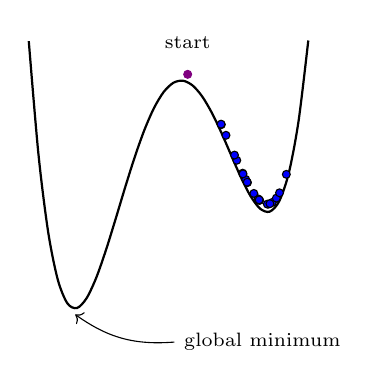
\begin{tikzpicture}
            \draw[thick,domain=-1.85:1.7, smooth, variable=\x,samples=30] plot ({\x}, {0.5*\x-3*\x*\x+\x*\x*\x*\x});
            \draw[violet,fill=violet] (0.168,0.1)node[black,above=0.2 cm]{\scriptsize start} circle (0.05);
            \foreach \i in {0,...,10}{
                \tikzmath{\x = rand*0.35+1.15;}
                \draw[fill=blue] (\x,0.1+0.5*\x-3*\x*\x+\x*\x*\x*\x) circle (0.05);
            }
            \foreach \i in {0,...,10}{
                \tikzmath{\x = rand*0.55+1.05;}
                \draw[fill=blue] (\x,0.1+0.5*\x-3*\x*\x+\x*\x*\x*\x) circle (0.05);
            }
            \draw[->] (0,-3.3)node[right]{\scriptsize global minimum}to[bend left=20](-1.26,-2.95);
        \end{tikzpicture}
        \caption{The system might appear to equilibrate inside the local well, even though our simulation is not sampling the phase space correctly. This is the \textit{ergodicity problem}: we cannot get everywhere in the phase space within the finite amount of simulation time.}
    \end{figure}

    One apparent solution to this ergodicity problem is to use brute force. If we run a large enough number of simulations from many different random initial conformations, then we would ultimately sample all over the phase space. However, we will introduce two other clever solutions that help us solve the ergodicity problem.
    \begin{enumerate}[topsep=0pt]
        \item Add a biasing potential and sample from a non-Boltzmann distribution so that the unfavorable states are sampled adequately.
        \item Enhance sampling by changing the kinetic energy of particles.
    \end{enumerate}
    Both methods help us climb over the potential barriers between minima.

    \subsubsection{Biased Sampling Methods}
    The standard (unbiased) canonical distribution is
    \begin{equation}
        P(i)\propto \exp[-\beta V(\vb{r}_i^N)]\,.
    \end{equation}
    In the biased ensemble, we introduce an additional weighting potential \(U\) for the microstates in the exponential
    \begin{equation}
        P_{\text{biased}}(i)\propto\exp[-\beta (V(\vb{r}_i^N)+U(\vb{r}_i^N))]\,.
    \end{equation}
    It modifies the canonical distribution so that some configurations can have higher or lower probabilities of being visited than they would normally do. If we compare the weighted and the unweighted probabilities, we get
    \begin{equation}
        \frac{P(i)}{P_{\text{biased}}(i)}=\exp[\beta U(\vb{r}_i^N)]\,.
    \end{equation}

    Using the biased property, we can follow our standard procedure in a Metropolis Monte Carlo simulation. We split the total transition probability into
    \begin{equation}
        W_{ij}=\alpha_{ij}P_{\text{acc}, ij}\,,
    \end{equation}
    and make the selection probability symmetric
    \begin{equation}
        \alpha_{ij}=\alpha_{ji}\,.
    \end{equation}
    Then by the detailed balance, we have
    \begin{equation}
        P_{\text{acc}, ij}=\min\{1,P_{\text{biased}}(j)/P_{\text{biased}}(i)\}=\min\{1,\exp[-\beta(\Delta V+\Delta U)]\}\,.
    \end{equation}
    Then to recover the ensemble average of a physical quantity in the standard canonical ensemble, we reweight the sampled microstates and get
    \begin{equation}
        \eval{A}=\frac{\sum_i A_i P(i)/P_{\text{biased}}(i)}{\sum_i P(i)/P_{\text{biased}}(i)}=\frac{\sum_i A_i\exp[\beta U(\vb{r}_i^N)]}{\sum_i\exp[\beta U(\vb{r}_i^N)]}\,.
    \end{equation}

    Since the introduction of biasing is to avoid ergodicity issues, we often choose \(U(\vb{r}_i^N)\) such that the simulation explores a wide range of microstates to accumulate a good statistics. We can think of them as artificially reshaping the free-energy landscape to improve sampling in specific regions. We will briefly introduce two common biasing methods: metadynamics and umbrella sampling.

    \subsubsection*{Metadynamics}
    Metadynamics tackles difficult-to-simulate systems by applying a history-dependent biasing potential that discourages the system from revisiting previously  explored states.
    \begin{enumerate}[topsep=0pt]
        \item A few low-dimensional reaction coordinates are chosen as \textit{collective variables} (CVs), \(\xi\) to describe the slow degrees of freedom which we plot our energy landscapes against.
        \item During the simulation, a small Gaussian potential is added to the potential energy of the system at the current position of the system in the CV space. This discourages the system from returning to the same region, pushing it into new unexplored states.
        \item Over time, the biased potential will ``fill in'' the local minima, flattening the energy landscape. The system is then driven over the energy barrier and is dropped into another minimum.
        \item The accumulated bias potential is related to the negative of the free energy landscape, allowing one to reconstruct the free-energy profile of the system.
    \end{enumerate}

    The biased potential at time \(t\) is given by
    \begin{equation}
        U(\xi,t)=\sum_{t'<t}w\ee^{-\frac{(\xi-\xi(t'))^2}{2\sigma^2}}\,,
    \end{equation}
    where \(w\) and \(\sigma\) are the height and width of the Gaussian bias potential added at each time step.
    
    \begin{figure}
        \centering
        % This file was created with tikzplotlib v0.10.1.
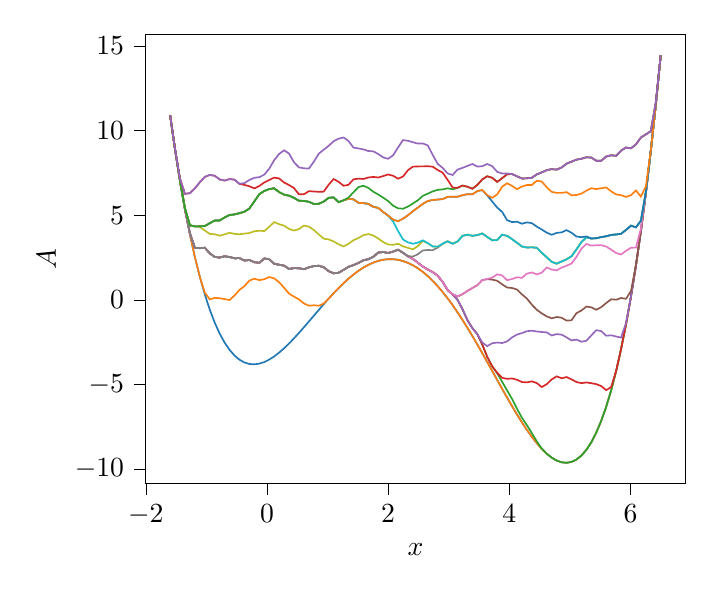
\begin{tikzpicture}

\definecolor{crimson2143940}{RGB}{214,39,40}
\definecolor{darkgray176}{RGB}{176,176,176}
\definecolor{darkorange25512714}{RGB}{255,127,14}
\definecolor{darkturquoise23190207}{RGB}{23,190,207}
\definecolor{forestgreen4416044}{RGB}{44,160,44}
\definecolor{goldenrod18818934}{RGB}{188,189,34}
\definecolor{gray127}{RGB}{127,127,127}
\definecolor{mediumpurple148103189}{RGB}{148,103,189}
\definecolor{orchid227119194}{RGB}{227,119,194}
\definecolor{sienna1408675}{RGB}{140,86,75}
\definecolor{steelblue31119180}{RGB}{31,119,180}

\begin{axis}[
tick align=outside,
tick pos=left,
x grid style={darkgray176},
xlabel={\(\displaystyle x\)},
xmin=-2.005, xmax=6.905,
xtick style={color=black},
y grid style={darkgray176},
ylabel={\(\displaystyle A\)},
ymin=-10.82845, ymax=15.64745,
ytick style={color=black}
]
\addplot [semithick, steelblue31119180]
table {%
-1.6 10.908
-1.518 8.865
-1.436 7.015
-1.355 5.347
-1.273 3.852
-1.191 2.521
-1.109 1.344
-1.027 0.313
-0.945 -0.582
-0.864 -1.348
-0.782 -1.994
-0.7 -2.529
-0.618 -2.959
-0.536 -3.293
-0.455 -3.538
-0.373 -3.701
-0.291 -3.79
-0.209 -3.811
-0.127 -3.77
-0.045 -3.675
0.036 -3.53
0.118 -3.343
0.2 -3.118
0.282 -2.862
0.364 -2.579
0.445 -2.275
0.527 -1.954
0.609 -1.621
0.691 -1.281
0.773 -0.938
0.855 -0.596
0.936 -0.258
1.018 0.072
1.1 0.391
1.182 0.695
1.264 0.982
1.345 1.248
1.427 1.492
1.509 1.711
1.591 1.902
1.673 2.065
1.755 2.198
1.836 2.299
1.918 2.366
2 2.4
2.082 2.399
2.164 2.362
2.245 2.29
2.327 2.182
2.409 2.039
2.491 1.86
2.573 1.646
2.655 1.398
2.736 1.116
2.818 0.803
2.9 0.459
2.982 0.087
3.064 -0.313
3.145 -0.739
3.227 -1.187
3.309 -1.655
3.391 -2.141
3.473 -2.643
3.555 -3.156
3.636 -3.677
3.718 -4.203
3.8 -4.731
3.882 -5.256
3.964 -5.773
4.045 -6.28
4.127 -6.77
4.209 -7.239
4.291 -7.683
4.373 -8.096
4.455 -8.472
4.536 -8.805
4.618 -9.091
4.7 -9.322
4.782 -9.492
4.864 -9.596
4.945 -9.625
5.027 -9.573
5.109 -9.434
5.191 -9.198
5.273 -8.86
5.355 -8.411
5.436 -7.842
5.518 -7.146
5.6 -6.315
5.682 -5.339
5.764 -4.209
5.845 -2.917
5.927 -1.453
6.009 0.192
6.091 2.029
6.173 4.067
6.255 6.316
6.336 8.787
6.418 11.491
6.5 14.438
};
\addplot [semithick, darkorange25512714]
table {%
-1.6 10.908
-1.518 8.865
-1.436 7.015
-1.355 5.347
-1.273 3.852
-1.191 2.521
-1.109 1.351
-1.027 0.419
-0.945 0.026
-0.864 0.114
-0.782 0.093
-0.7 0.041
-0.618 -0.013
-0.536 0.26
-0.455 0.587
-0.373 0.81
-0.291 1.133
-0.209 1.246
-0.127 1.161
-0.045 1.216
0.036 1.343
0.118 1.266
0.2 1.038
0.282 0.709
0.364 0.363
0.445 0.186
0.527 0.027
0.609 -0.216
0.691 -0.348
0.773 -0.322
0.855 -0.35
0.936 -0.224
1.018 0.074
1.1 0.391
1.182 0.695
1.264 0.982
1.345 1.248
1.427 1.492
1.509 1.711
1.591 1.902
1.673 2.065
1.755 2.198
1.836 2.299
1.918 2.366
2 2.4
2.082 2.399
2.164 2.362
2.245 2.29
2.327 2.182
2.409 2.039
2.491 1.86
2.573 1.646
2.655 1.398
2.736 1.116
2.818 0.803
2.9 0.459
2.982 0.087
3.064 -0.313
3.145 -0.739
3.227 -1.187
3.309 -1.655
3.391 -2.141
3.473 -2.643
3.555 -3.156
3.636 -3.677
3.718 -4.203
3.8 -4.731
3.882 -5.256
3.964 -5.773
4.045 -6.28
4.127 -6.77
4.209 -7.239
4.291 -7.683
4.373 -8.096
4.455 -8.472
4.536 -8.805
4.618 -9.091
4.7 -9.322
4.782 -9.492
4.864 -9.596
4.945 -9.625
5.027 -9.573
5.109 -9.434
5.191 -9.198
5.273 -8.86
5.355 -8.411
5.436 -7.842
5.518 -7.146
5.6 -6.315
5.682 -5.339
5.764 -4.209
5.845 -2.917
5.927 -1.453
6.009 0.192
6.091 2.029
6.173 4.067
6.255 6.316
6.336 8.787
6.418 11.491
6.5 14.438
};
\addplot [semithick, forestgreen4416044]
table {%
-1.6 10.908
-1.518 8.865
-1.436 7.015
-1.355 5.35
-1.273 3.921
-1.191 3.07
-1.109 3.049
-1.027 3.073
-0.945 2.742
-0.864 2.532
-0.782 2.495
-0.7 2.574
-0.618 2.525
-0.536 2.453
-0.455 2.464
-0.373 2.319
-0.291 2.353
-0.209 2.219
-0.127 2.19
-0.045 2.44
0.036 2.395
0.118 2.128
0.2 2.07
0.282 2.019
0.364 1.82
0.445 1.872
0.527 1.865
0.609 1.806
0.691 1.916
0.773 1.992
0.855 2.011
0.936 1.924
1.018 1.689
1.1 1.567
1.182 1.598
1.264 1.77
1.345 1.945
1.427 2.05
1.509 2.175
1.591 2.332
1.673 2.398
1.755 2.54
1.836 2.788
1.918 2.823
2 2.764
2.082 2.847
2.164 2.959
2.245 2.776
2.327 2.567
2.409 2.413
2.491 2.186
2.573 1.962
2.655 1.785
2.736 1.636
2.818 1.427
2.9 1.053
2.982 0.573
3.064 0.316
3.145 0.003
3.227 -0.551
3.309 -1.207
3.391 -1.673
3.473 -2.035
3.555 -2.649
3.636 -3.378
3.718 -3.931
3.8 -4.34
3.882 -4.843
3.964 -5.352
4.045 -5.852
4.127 -6.428
4.209 -6.969
4.291 -7.405
4.373 -7.871
4.455 -8.371
4.536 -8.785
4.618 -9.089
4.7 -9.322
4.782 -9.492
4.864 -9.596
4.945 -9.625
5.027 -9.573
5.109 -9.434
5.191 -9.198
5.273 -8.86
5.355 -8.411
5.436 -7.842
5.518 -7.146
5.6 -6.315
5.682 -5.339
5.764 -4.209
5.845 -2.917
5.927 -1.453
6.009 0.192
6.091 2.029
6.173 4.067
6.255 6.316
6.336 8.787
6.418 11.491
6.5 14.438
};
\addplot [semithick, crimson2143940]
table {%
-1.6 10.908
-1.518 8.865
-1.436 7.015
-1.355 5.35
-1.273 3.921
-1.191 3.07
-1.109 3.049
-1.027 3.073
-0.945 2.742
-0.864 2.532
-0.782 2.495
-0.7 2.574
-0.618 2.525
-0.536 2.453
-0.455 2.464
-0.373 2.319
-0.291 2.353
-0.209 2.219
-0.127 2.19
-0.045 2.44
0.036 2.395
0.118 2.128
0.2 2.07
0.282 2.019
0.364 1.82
0.445 1.872
0.527 1.865
0.609 1.806
0.691 1.916
0.773 1.992
0.855 2.011
0.936 1.924
1.018 1.689
1.1 1.567
1.182 1.598
1.264 1.77
1.345 1.945
1.427 2.05
1.509 2.175
1.591 2.332
1.673 2.398
1.755 2.54
1.836 2.788
1.918 2.823
2 2.764
2.082 2.847
2.164 2.959
2.245 2.776
2.327 2.567
2.409 2.413
2.491 2.186
2.573 1.962
2.655 1.785
2.736 1.636
2.818 1.427
2.9 1.053
2.982 0.573
3.064 0.316
3.145 0.003
3.227 -0.551
3.309 -1.207
3.391 -1.673
3.473 -2.035
3.555 -2.649
3.636 -3.378
3.718 -3.93
3.8 -4.308
3.882 -4.607
3.964 -4.668
4.045 -4.644
4.127 -4.722
4.209 -4.856
4.291 -4.877
4.373 -4.816
4.455 -4.919
4.536 -5.153
4.618 -4.982
4.7 -4.701
4.782 -4.521
4.864 -4.633
4.945 -4.561
5.027 -4.698
5.109 -4.855
5.191 -4.921
5.273 -4.88
5.355 -4.926
5.436 -4.98
5.518 -5.095
5.6 -5.337
5.682 -5.145
5.764 -4.197
5.845 -2.917
5.927 -1.453
6.009 0.192
6.091 2.029
6.173 4.067
6.255 6.316
6.336 8.787
6.418 11.491
6.5 14.438
};
\addplot [semithick, mediumpurple148103189]
table {%
-1.6 10.908
-1.518 8.865
-1.436 7.015
-1.355 5.35
-1.273 3.921
-1.191 3.07
-1.109 3.049
-1.027 3.073
-0.945 2.742
-0.864 2.532
-0.782 2.495
-0.7 2.574
-0.618 2.525
-0.536 2.453
-0.455 2.464
-0.373 2.319
-0.291 2.353
-0.209 2.219
-0.127 2.19
-0.045 2.44
0.036 2.395
0.118 2.128
0.2 2.07
0.282 2.019
0.364 1.82
0.445 1.872
0.527 1.865
0.609 1.806
0.691 1.916
0.773 1.992
0.855 2.011
0.936 1.924
1.018 1.689
1.1 1.567
1.182 1.598
1.264 1.77
1.345 1.945
1.427 2.05
1.509 2.175
1.591 2.332
1.673 2.398
1.755 2.54
1.836 2.788
1.918 2.823
2 2.764
2.082 2.847
2.164 2.959
2.245 2.776
2.327 2.567
2.409 2.413
2.491 2.186
2.573 1.962
2.655 1.785
2.736 1.636
2.818 1.427
2.9 1.053
2.982 0.573
3.064 0.316
3.145 0.003
3.227 -0.551
3.309 -1.207
3.391 -1.673
3.473 -2.027
3.555 -2.528
3.636 -2.734
3.718 -2.564
3.8 -2.525
3.882 -2.551
3.964 -2.454
4.045 -2.222
4.127 -2.052
4.209 -1.964
4.291 -1.853
4.373 -1.826
4.455 -1.872
4.536 -1.901
4.618 -1.922
4.7 -2.108
4.782 -2.025
4.864 -2.058
4.945 -2.217
5.027 -2.398
5.109 -2.35
5.191 -2.475
5.273 -2.417
5.355 -2.099
5.436 -1.794
5.518 -1.848
5.6 -2.121
5.682 -2.097
5.764 -2.166
5.845 -2.232
5.927 -1.365
6.009 0.196
6.091 2.029
6.173 4.067
6.255 6.316
6.336 8.787
6.418 11.491
6.5 14.438
};
\addplot [semithick, sienna1408675]
table {%
-1.6 10.908
-1.518 8.865
-1.436 7.015
-1.355 5.35
-1.273 3.921
-1.191 3.07
-1.109 3.049
-1.027 3.073
-0.945 2.742
-0.864 2.532
-0.782 2.495
-0.7 2.574
-0.618 2.525
-0.536 2.453
-0.455 2.464
-0.373 2.319
-0.291 2.353
-0.209 2.219
-0.127 2.19
-0.045 2.44
0.036 2.395
0.118 2.128
0.2 2.07
0.282 2.019
0.364 1.82
0.445 1.872
0.527 1.865
0.609 1.806
0.691 1.916
0.773 1.992
0.855 2.011
0.936 1.924
1.018 1.689
1.1 1.567
1.182 1.598
1.264 1.77
1.345 1.945
1.427 2.05
1.509 2.175
1.591 2.332
1.673 2.398
1.755 2.54
1.836 2.788
1.918 2.823
2 2.764
2.082 2.847
2.164 2.959
2.245 2.776
2.327 2.567
2.409 2.413
2.491 2.186
2.573 1.962
2.655 1.785
2.736 1.636
2.818 1.427
2.9 1.053
2.982 0.573
3.064 0.33
3.145 0.203
3.227 0.328
3.309 0.524
3.391 0.697
3.473 0.865
3.555 1.169
3.636 1.215
3.718 1.192
3.8 1.124
3.882 0.915
3.964 0.724
4.045 0.698
4.127 0.607
4.209 0.32
4.291 0.072
4.373 -0.288
4.455 -0.592
4.536 -0.803
4.618 -0.979
4.7 -1.095
4.782 -1.014
4.864 -1.058
4.945 -1.228
5.027 -1.21
5.109 -0.787
5.191 -0.633
5.273 -0.398
5.355 -0.445
5.436 -0.59
5.518 -0.434
5.6 -0.188
5.682 0.031
5.764 0.007
5.845 0.106
5.927 0.059
6.009 0.518
6.091 2.052
6.173 4.067
6.255 6.316
6.336 8.787
6.418 11.491
6.5 14.438
};
\addplot [semithick, orchid227119194]
table {%
-1.6 10.908
-1.518 8.865
-1.436 7.015
-1.355 5.35
-1.273 3.921
-1.191 3.07
-1.109 3.049
-1.027 3.073
-0.945 2.742
-0.864 2.532
-0.782 2.495
-0.7 2.574
-0.618 2.525
-0.536 2.453
-0.455 2.464
-0.373 2.319
-0.291 2.353
-0.209 2.219
-0.127 2.19
-0.045 2.44
0.036 2.395
0.118 2.128
0.2 2.07
0.282 2.019
0.364 1.82
0.445 1.872
0.527 1.865
0.609 1.806
0.691 1.916
0.773 1.992
0.855 2.011
0.936 1.924
1.018 1.689
1.1 1.567
1.182 1.598
1.264 1.77
1.345 1.945
1.427 2.05
1.509 2.175
1.591 2.332
1.673 2.398
1.755 2.54
1.836 2.788
1.918 2.823
2 2.764
2.082 2.847
2.164 2.959
2.245 2.776
2.327 2.567
2.409 2.413
2.491 2.186
2.573 1.962
2.655 1.785
2.736 1.636
2.818 1.427
2.9 1.053
2.982 0.573
3.064 0.33
3.145 0.203
3.227 0.328
3.309 0.524
3.391 0.697
3.473 0.865
3.555 1.169
3.636 1.229
3.718 1.311
3.8 1.506
3.882 1.437
3.964 1.158
4.045 1.229
4.127 1.33
4.209 1.295
4.291 1.548
4.373 1.616
4.455 1.499
4.536 1.604
4.618 1.91
4.7 1.786
4.782 1.737
4.864 1.903
4.945 2.013
5.027 2.143
5.109 2.533
5.191 3.02
5.273 3.301
5.355 3.198
5.436 3.223
5.518 3.228
5.6 3.143
5.682 2.964
5.764 2.763
5.845 2.675
5.927 2.892
6.009 3.075
6.091 3.083
6.173 4.212
6.255 6.322
6.336 8.787
6.418 11.491
6.5 14.438
};
\addplot [semithick, gray127]
table {%
-1.6 10.908
-1.518 8.865
-1.436 7.015
-1.355 5.35
-1.273 3.921
-1.191 3.07
-1.109 3.049
-1.027 3.073
-0.945 2.742
-0.864 2.532
-0.782 2.495
-0.7 2.574
-0.618 2.525
-0.536 2.453
-0.455 2.464
-0.373 2.319
-0.291 2.353
-0.209 2.219
-0.127 2.19
-0.045 2.44
0.036 2.395
0.118 2.128
0.2 2.07
0.282 2.019
0.364 1.82
0.445 1.872
0.527 1.865
0.609 1.806
0.691 1.916
0.773 1.992
0.855 2.011
0.936 1.924
1.018 1.689
1.1 1.567
1.182 1.598
1.264 1.77
1.345 1.945
1.427 2.05
1.509 2.175
1.591 2.332
1.673 2.398
1.755 2.54
1.836 2.788
1.918 2.823
2 2.764
2.082 2.847
2.164 2.959
2.245 2.777
2.327 2.584
2.409 2.554
2.491 2.695
2.573 2.917
2.655 2.941
2.736 2.931
2.818 3.083
2.9 3.312
2.982 3.454
3.064 3.313
3.145 3.441
3.227 3.778
3.309 3.849
3.391 3.778
3.473 3.824
3.555 3.917
3.636 3.708
3.718 3.517
3.8 3.53
3.882 3.847
3.964 3.774
4.045 3.581
4.127 3.37
4.209 3.148
4.291 3.088
4.373 3.1
4.455 3.07
4.536 2.777
4.618 2.515
4.7 2.242
4.782 2.133
4.864 2.265
4.945 2.389
5.027 2.57
5.109 2.978
5.191 3.408
5.273 3.694
5.355 3.618
5.436 3.638
5.518 3.705
5.6 3.751
5.682 3.831
5.764 3.86
5.845 3.896
5.927 4.127
6.009 4.381
6.091 4.281
6.173 4.673
6.255 6.377
6.336 8.789
6.418 11.491
6.5 14.438
};
\addplot [semithick, goldenrod18818934]
table {%
-1.6 10.908
-1.518 8.865
-1.436 7.017
-1.355 5.406
-1.273 4.402
-1.191 4.332
-1.109 4.303
-1.027 4.09
-0.945 3.892
-0.864 3.871
-0.782 3.786
-0.7 3.866
-0.618 3.962
-0.536 3.892
-0.455 3.873
-0.373 3.908
-0.291 3.942
-0.209 4.051
-0.127 4.077
-0.045 4.061
0.036 4.317
0.118 4.588
0.2 4.465
0.282 4.379
0.364 4.187
0.445 4.09
0.527 4.176
0.609 4.383
0.691 4.32
0.773 4.122
0.855 3.861
0.936 3.614
1.018 3.564
1.1 3.447
1.182 3.275
1.264 3.153
1.345 3.308
1.427 3.519
1.509 3.648
1.591 3.821
1.673 3.883
1.755 3.8
1.836 3.62
1.918 3.408
2 3.266
2.082 3.247
2.164 3.307
2.245 3.157
2.327 3.068
2.409 2.983
2.491 3.177
2.573 3.471
2.655 3.343
2.736 3.152
2.818 3.139
2.9 3.316
2.982 3.454
3.064 3.313
3.145 3.441
3.227 3.778
3.309 3.849
3.391 3.778
3.473 3.824
3.555 3.917
3.636 3.708
3.718 3.517
3.8 3.53
3.882 3.847
3.964 3.774
4.045 3.581
4.127 3.37
4.209 3.148
4.291 3.088
4.373 3.1
4.455 3.07
4.536 2.777
4.618 2.515
4.7 2.242
4.782 2.133
4.864 2.265
4.945 2.389
5.027 2.57
5.109 2.978
5.191 3.408
5.273 3.694
5.355 3.618
5.436 3.638
5.518 3.705
5.6 3.751
5.682 3.831
5.764 3.86
5.845 3.896
5.927 4.127
6.009 4.381
6.091 4.281
6.173 4.673
6.255 6.377
6.336 8.789
6.418 11.491
6.5 14.438
};
\addplot [semithick, darkturquoise23190207]
table {%
-1.6 10.908
-1.518 8.865
-1.436 7.017
-1.355 5.406
-1.273 4.402
-1.191 4.334
-1.109 4.343
-1.027 4.357
-0.945 4.524
-0.864 4.684
-0.782 4.686
-0.7 4.863
-0.618 5.008
-0.536 5.044
-0.455 5.117
-0.373 5.203
-0.291 5.391
-0.209 5.813
-0.127 6.241
-0.045 6.428
0.036 6.539
0.118 6.587
0.2 6.359
0.282 6.211
0.364 6.147
0.445 6.021
0.527 5.848
0.609 5.842
0.691 5.788
0.773 5.659
0.855 5.672
0.936 5.802
1.018 6.023
1.1 6.049
1.182 5.766
1.264 5.875
1.345 5.968
1.427 5.932
1.509 5.729
1.591 5.708
1.673 5.667
1.755 5.49
1.836 5.429
1.918 5.182
2 4.968
2.082 4.62
2.164 4.059
2.245 3.565
2.327 3.391
2.409 3.311
2.491 3.38
2.573 3.512
2.655 3.345
2.736 3.152
2.818 3.139
2.9 3.316
2.982 3.454
3.064 3.313
3.145 3.441
3.227 3.778
3.309 3.849
3.391 3.778
3.473 3.824
3.555 3.917
3.636 3.708
3.718 3.517
3.8 3.53
3.882 3.847
3.964 3.774
4.045 3.581
4.127 3.37
4.209 3.148
4.291 3.088
4.373 3.1
4.455 3.07
4.536 2.777
4.618 2.515
4.7 2.242
4.782 2.133
4.864 2.265
4.945 2.389
5.027 2.57
5.109 2.978
5.191 3.408
5.273 3.694
5.355 3.618
5.436 3.638
5.518 3.705
5.6 3.751
5.682 3.831
5.764 3.86
5.845 3.896
5.927 4.127
6.009 4.381
6.091 4.281
6.173 4.673
6.255 6.377
6.336 8.789
6.418 11.491
6.5 14.438
};
\addplot [semithick, steelblue31119180]
table {%
-1.6 10.908
-1.518 8.865
-1.436 7.017
-1.355 5.406
-1.273 4.402
-1.191 4.334
-1.109 4.343
-1.027 4.357
-0.945 4.524
-0.864 4.684
-0.782 4.686
-0.7 4.863
-0.618 5.008
-0.536 5.044
-0.455 5.117
-0.373 5.203
-0.291 5.391
-0.209 5.813
-0.127 6.241
-0.045 6.428
0.036 6.539
0.118 6.587
0.2 6.359
0.282 6.211
0.364 6.147
0.445 6.021
0.527 5.848
0.609 5.842
0.691 5.788
0.773 5.659
0.855 5.672
0.936 5.802
1.018 6.023
1.1 6.049
1.182 5.766
1.264 5.875
1.345 5.968
1.427 5.932
1.509 5.729
1.591 5.708
1.673 5.667
1.755 5.49
1.836 5.429
1.918 5.182
2 4.976
2.082 4.735
2.164 4.644
2.245 4.792
2.327 4.992
2.409 5.237
2.491 5.446
2.573 5.669
2.655 5.835
2.736 5.896
2.818 5.92
2.9 5.951
2.982 6.079
3.064 6.091
3.145 6.09
3.227 6.179
3.309 6.238
3.391 6.234
3.473 6.419
3.555 6.483
3.636 6.164
3.718 5.804
3.8 5.447
3.882 5.191
3.964 4.702
4.045 4.59
4.127 4.614
4.209 4.493
4.291 4.573
4.373 4.526
4.455 4.319
4.536 4.151
4.618 3.966
4.7 3.842
4.782 3.951
4.864 3.983
4.945 4.116
5.027 3.96
5.109 3.737
5.191 3.699
5.273 3.743
5.355 3.62
5.436 3.638
5.518 3.705
5.6 3.751
5.682 3.831
5.764 3.86
5.845 3.896
5.927 4.127
6.009 4.381
6.091 4.281
6.173 4.673
6.255 6.377
6.336 8.789
6.418 11.491
6.5 14.438
};
\addplot [semithick, darkorange25512714]
table {%
-1.6 10.908
-1.518 8.865
-1.436 7.017
-1.355 5.406
-1.273 4.402
-1.191 4.334
-1.109 4.343
-1.027 4.357
-0.945 4.524
-0.864 4.684
-0.782 4.686
-0.7 4.863
-0.618 5.008
-0.536 5.044
-0.455 5.117
-0.373 5.203
-0.291 5.391
-0.209 5.813
-0.127 6.241
-0.045 6.428
0.036 6.539
0.118 6.587
0.2 6.359
0.282 6.211
0.364 6.147
0.445 6.021
0.527 5.848
0.609 5.842
0.691 5.788
0.773 5.659
0.855 5.672
0.936 5.802
1.018 6.023
1.1 6.049
1.182 5.766
1.264 5.875
1.345 5.968
1.427 5.932
1.509 5.729
1.591 5.708
1.673 5.667
1.755 5.49
1.836 5.429
1.918 5.182
2 4.976
2.082 4.735
2.164 4.644
2.245 4.792
2.327 4.992
2.409 5.237
2.491 5.446
2.573 5.669
2.655 5.835
2.736 5.896
2.818 5.92
2.9 5.951
2.982 6.079
3.064 6.091
3.145 6.09
3.227 6.179
3.309 6.238
3.391 6.234
3.473 6.419
3.555 6.483
3.636 6.185
3.718 6.021
3.8 6.225
3.882 6.679
3.964 6.884
4.045 6.729
4.127 6.534
4.209 6.69
4.291 6.781
4.373 6.784
4.455 7.035
4.536 6.982
4.618 6.648
4.7 6.373
4.782 6.316
4.864 6.315
4.945 6.358
5.027 6.173
5.109 6.191
5.191 6.272
5.273 6.447
5.355 6.592
5.436 6.538
5.518 6.588
5.6 6.639
5.682 6.404
5.764 6.225
5.845 6.179
5.927 6.078
6.009 6.178
6.091 6.457
6.173 6.098
6.255 6.696
6.336 8.811
6.418 11.491
6.5 14.438
};
\addplot [semithick, forestgreen4416044]
table {%
-1.6 10.908
-1.518 8.865
-1.436 7.017
-1.355 5.406
-1.273 4.402
-1.191 4.334
-1.109 4.343
-1.027 4.357
-0.945 4.524
-0.864 4.684
-0.782 4.686
-0.7 4.863
-0.618 5.008
-0.536 5.044
-0.455 5.117
-0.373 5.203
-0.291 5.391
-0.209 5.813
-0.127 6.241
-0.045 6.428
0.036 6.539
0.118 6.587
0.2 6.359
0.282 6.211
0.364 6.147
0.445 6.021
0.527 5.848
0.609 5.842
0.691 5.788
0.773 5.659
0.855 5.672
0.936 5.802
1.018 6.023
1.1 6.049
1.182 5.766
1.264 5.879
1.345 6.038
1.427 6.352
1.509 6.654
1.591 6.738
1.673 6.607
1.755 6.381
1.836 6.221
1.918 6.031
2 5.832
2.082 5.558
2.164 5.403
2.245 5.378
2.327 5.506
2.409 5.687
2.491 5.88
2.573 6.14
2.655 6.272
2.736 6.403
2.818 6.494
2.9 6.521
2.982 6.584
3.064 6.526
3.145 6.607
3.227 6.747
3.309 6.678
3.391 6.558
3.473 6.789
3.555 7.112
3.636 7.296
3.718 7.206
3.8 6.961
3.882 7.183
3.964 7.415
4.045 7.424
4.127 7.296
4.209 7.163
4.291 7.175
4.373 7.209
4.455 7.41
4.536 7.527
4.618 7.655
4.7 7.717
4.782 7.688
4.864 7.815
4.945 8.039
5.027 8.158
5.109 8.277
5.191 8.33
5.273 8.418
5.355 8.399
5.436 8.214
5.518 8.21
5.6 8.46
5.682 8.534
5.764 8.506
5.845 8.81
5.927 8.993
6.009 8.949
6.091 9.177
6.173 9.585
6.255 9.769
6.336 9.959
6.418 11.645
6.5 14.444
};
\addplot [semithick, crimson2143940]
table {%
-1.6 10.908
-1.518 8.872
-1.436 7.153
-1.355 6.257
-1.273 6.299
-1.191 6.581
-1.109 6.945
-1.027 7.261
-0.945 7.373
-0.864 7.327
-0.782 7.107
-0.7 7.043
-0.618 7.13
-0.536 7.095
-0.455 6.842
-0.373 6.784
-0.291 6.705
-0.209 6.58
-0.127 6.723
-0.045 6.933
0.036 7.073
0.118 7.217
0.2 7.167
0.282 6.925
0.364 6.776
0.445 6.601
0.527 6.228
0.609 6.233
0.691 6.415
0.773 6.398
0.855 6.375
0.936 6.388
1.018 6.8
1.1 7.133
1.182 6.968
1.264 6.734
1.345 6.791
1.427 7.115
1.509 7.156
1.591 7.136
1.673 7.223
1.755 7.258
1.836 7.222
1.918 7.307
2 7.401
2.082 7.324
2.164 7.152
2.245 7.279
2.327 7.655
2.409 7.863
2.491 7.877
2.573 7.878
2.655 7.892
2.736 7.858
2.818 7.665
2.9 7.506
2.982 7.085
3.064 6.631
3.145 6.615
3.227 6.747
3.309 6.678
3.391 6.558
3.473 6.789
3.555 7.112
3.636 7.296
3.718 7.206
3.8 6.961
3.882 7.183
3.964 7.415
4.045 7.424
4.127 7.296
4.209 7.163
4.291 7.175
4.373 7.209
4.455 7.41
4.536 7.527
4.618 7.655
4.7 7.717
4.782 7.688
4.864 7.815
4.945 8.039
5.027 8.158
5.109 8.277
5.191 8.33
5.273 8.418
5.355 8.399
5.436 8.214
5.518 8.21
5.6 8.46
5.682 8.534
5.764 8.506
5.845 8.81
5.927 8.993
6.009 8.949
6.091 9.177
6.173 9.585
6.255 9.769
6.336 9.959
6.418 11.645
6.5 14.444
};
\addplot [semithick, mediumpurple148103189]
table {%
-1.6 10.908
-1.518 8.872
-1.436 7.153
-1.355 6.257
-1.273 6.299
-1.191 6.581
-1.109 6.945
-1.027 7.261
-0.945 7.373
-0.864 7.327
-0.782 7.107
-0.7 7.043
-0.618 7.13
-0.536 7.095
-0.455 6.855
-0.373 6.89
-0.291 7.08
-0.209 7.205
-0.127 7.243
-0.045 7.391
0.036 7.742
0.118 8.244
0.2 8.615
0.282 8.828
0.364 8.635
0.445 8.123
0.527 7.82
0.609 7.768
0.691 7.748
0.773 8.157
0.855 8.633
0.936 8.865
1.018 9.094
1.1 9.366
1.182 9.518
1.264 9.586
1.345 9.379
1.427 8.99
1.509 8.939
1.591 8.881
1.673 8.788
1.755 8.765
1.836 8.611
1.918 8.408
2 8.329
2.082 8.536
2.164 9.003
2.245 9.432
2.327 9.391
2.409 9.305
2.491 9.227
2.573 9.233
2.655 9.115
2.736 8.553
2.818 8.025
2.9 7.789
2.982 7.462
3.064 7.368
3.145 7.69
3.227 7.792
3.309 7.908
3.391 8.02
3.473 7.869
3.555 7.889
3.636 8.022
3.718 7.891
3.8 7.561
3.882 7.46
3.964 7.464
4.045 7.428
4.127 7.296
4.209 7.163
4.291 7.175
4.373 7.209
4.455 7.41
4.536 7.527
4.618 7.655
4.7 7.717
4.782 7.688
4.864 7.815
4.945 8.039
5.027 8.158
5.109 8.277
5.191 8.33
5.273 8.418
5.355 8.399
5.436 8.214
5.518 8.21
5.6 8.46
5.682 8.534
5.764 8.506
5.845 8.81
5.927 8.993
6.009 8.949
6.091 9.177
6.173 9.585
6.255 9.769
6.336 9.959
6.418 11.645
6.5 14.444
};
\end{axis}

\end{tikzpicture}

        \vskip -20 pt
        \caption{Energy landscapes of the system against Monte Carlo steps (1,000 steps between consecutive plots) in a metadynamics simulation.}
    \end{figure}

    The free energy of a state is related to its probability by
    \begin{equation}
        A(\xi)=-k_B T\ln P(\xi)\,.
    \end{equation}
    In metadynamics,
    \begin{equation}
        A_{\text{biased}}(\xi,t)=A_{\text{unbiased}}(\xi)+U(\xi,t)\,.
    \end{equation}
    In the limit of long simulation time, the landscape is completely filled, making all states equiprobable, and so
    \begin{equation}
        \lim_{t\to\infty}\ln P_{\text{biased}}(\xi,t)=-\beta\left[A_{\text{unbiased}}(\xi)+\lim_{t\to\infty} U(\xi,t)\right]=\text{const.}
    \end{equation}
    The constant shift in the free energy is unimportant. Therefore we can take
    \begin{equation}
        A_{\text{unbiased}}(\xi)=-\lim_{t\to\infty}U(\xi,t)\,.
    \end{equation}
    Various other quantities can then be derived, for example
    \begin{align}
        S(\xi)&=-\pdv{A(\xi)}{T}\\
        E(\xi)&=A(\xi)+TS(\xi)\\
        K&=\exp\left(-\frac{\Delta A}{k_B T}\right)\\
        k&=A\exp\left(-\frac{\Delta A^\ddagger}{k_B T}\right)\,.
    \end{align}
    Since the unbiased probability distribution is
    \begin{equation}
        P_{\text{unbiased}}=P_{\text{biased}}(\xi)\ee^{\beta U(\xi)}\,,
    \end{equation}
    for any physical quantity \(A\), the unbiased ensemble average can be computed as
    \begin{equation}
        \eval{A}=\frac{\sum_i A(\vb{r}_i)\ee^{\beta U(\xi_i)}}{\sum_i \ee^{\beta U(\xi_i)}}\,.
    \end{equation}

    \subsubsection*{Umbrella Sampling}
    In contrast to metadynamics, in umbrella sampling, we need to know the states \(A\) and \(B\) we want to connect, and then we define a \textit{reaction coordinate} \(\xi\) to connect these two states. We proceed as follows:
    \begin{enumerate}[topsep=0pt]
        \item We perform \(J\) simulations of the same system.
        \item In each simulation, we restrain the system to sample a small range of the reaction coordinate \(\xi\) centred around \(\xi_j\). This is done by adding a bias potential \(U_j(\xi)\), which can for example be a harmonic potential \(U_j(\xi)=\frac{1}{2}k(\xi-\xi_j)^2\).
        \item Use different target value \(\xi_j\) for each simulation such that it spans the entire range of interest.
        \item Measure the weighted ensemble distribution \(P_{\text{biased}}(\xi)\) for each simulation. Unweight and stitch together all \(P_{\text{biased}}(\xi)\) to produce an unweighted underlying free function.
    \end{enumerate}

    \begin{figure}
        \centering
        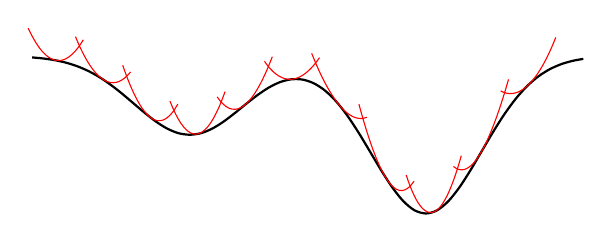
\begin{tikzpicture}
            \draw[thick,domain=-2:5, smooth, variable=\x,samples=50] plot ({\x}, {-2.72^(-\x*\x)-2*2.72^(-(\x-3)*(\x-3))});
            \foreach \i in {-1.7,-1.1,...,4.7}{
                \draw[red,domain=\i-0.35:\i+0.35, smooth, variable=\x,samples=20] plot ({\x}, {-2.72^(-\x*\x)-2*2.72^(-(\x-3)*(\x-3))+3*(\x-\i)*(\x-\i)});
            }
        \end{tikzpicture}
        \caption{Umbrella sampling adds a local harmonic biasing potential in each run.}
    \end{figure}

    Each simulation is connected to the unweighted distribution by
    \begin{equation}
        P(\vb{r}^N)\propto P_{\text{biased}, j}(\vb{r}^N)\exp[\beta U_j(\xi)]\,.
    \end{equation}
    By integrating all other coordinates except the reaction coordinate of interest, one can write
    \begin{equation}
        P(\xi)\propto P_{\text{biased}, j}(\xi)\exp[\beta U_j(\xi)]\,.
    \end{equation}
    Taking the logarithm gives
    \begin{equation}
        A(\xi)=-k_B T\ln[P_{\text{biased}, j}(\xi)]-U_j(\xi)+\text{const.}
    \end{equation}
    We can adjust the constant to glue different segments of \(A(\xi)\) together.

    \begin{figure}
        \centering
        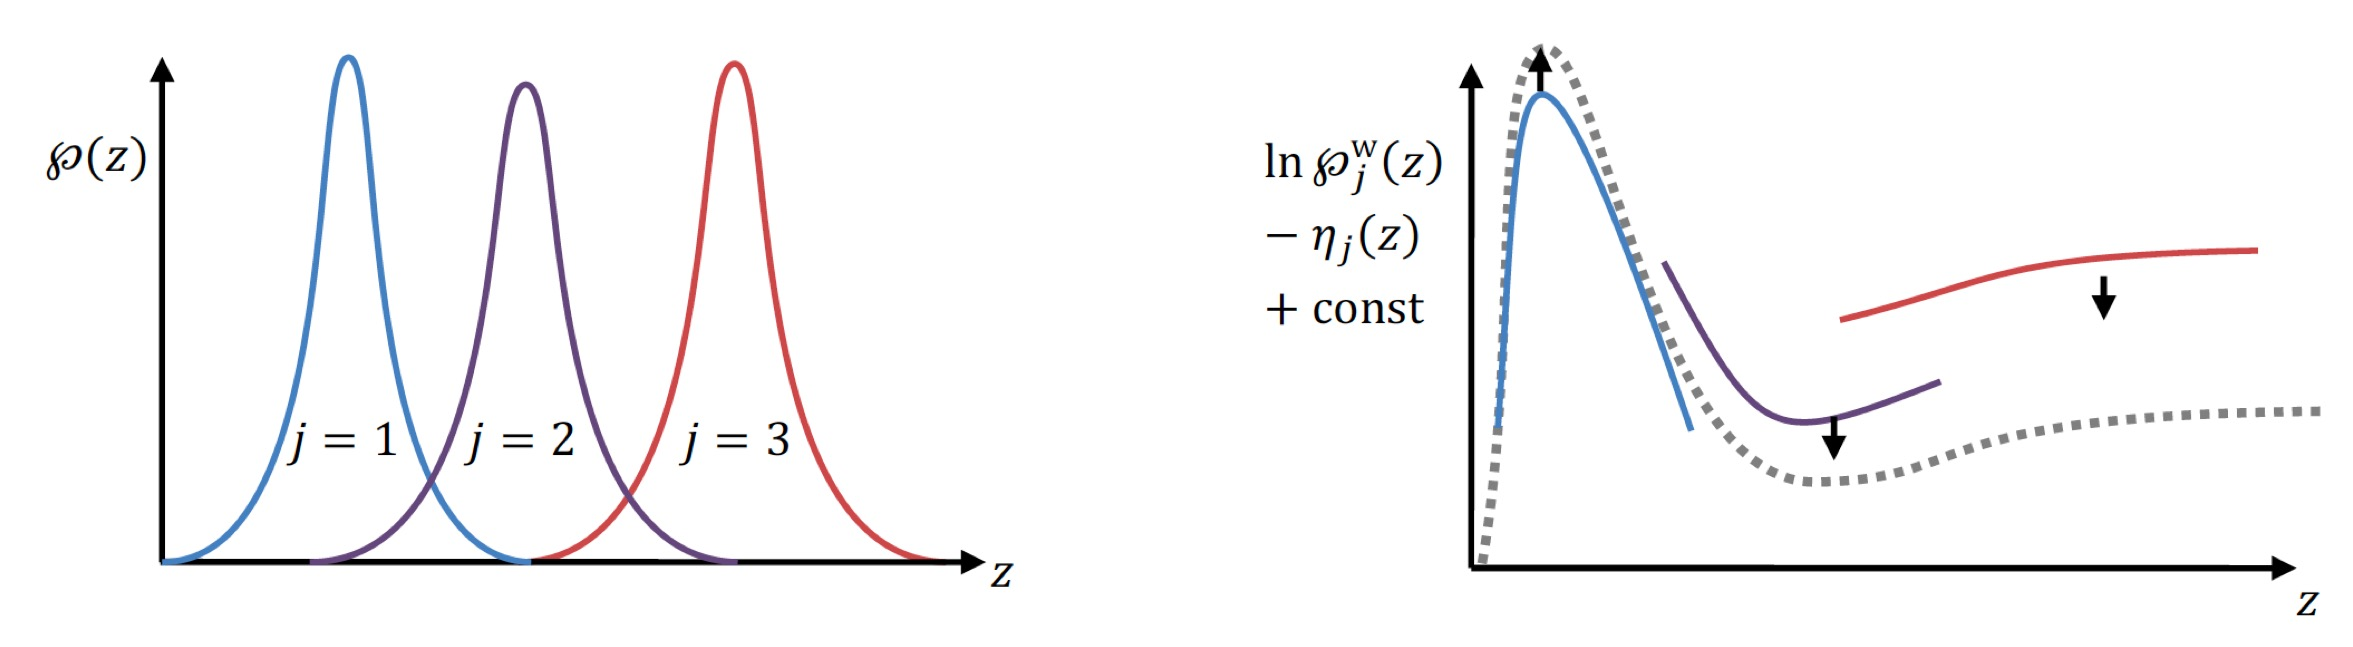
\includegraphics[width=0.8\textwidth]{Umbrella.jpg}
        \caption{Using umbrella sampling to construct the free energy landscape.}
    \end{figure}

    \subsubsection{Temperature Replica Exchange Molecular Dynamics}
    The next method uses high temperature to avoid being trapped in a local minimum. It is known as \textit{temperature replica exchange molecular dynamics} (T-REMD) (or the corresponding Monte Carlo). Suppose we want to investigate the system at temperature \(T_1\).
    \begin{enumerate}[topsep=0pt]
        \item We create \(J\) replicas of the same system, and perform them simultaneously at different temperature \(T_j\) with \(T_1<T_2<\dots<T_J\).
        \item Each simulation is evolved independently, either through MD or MC.
        \item At set intervals, \textit{replica swap MC moves} are performed between adjacent replicas. In a swap move, the instantaneous configurations are exchanged between the two temperatures.
    \end{enumerate}
    
    \begin{figure}
        \centering
        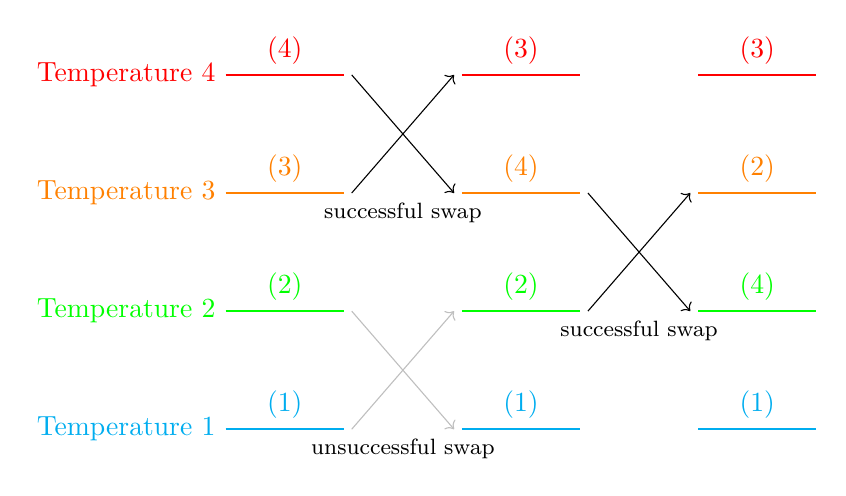
\begin{tikzpicture}
            \draw[cyan,thick] (0,0)node[left]{Temperature 1}--node[above]{(1)}(1.5,0);
            \draw[green,thick] (0,1.5)node[left]{Temperature 2}--node[above]{(2)}(1.5,1.5);
            \draw[orange,thick] (0,3)node[left]{Temperature 3}--node[above]{(3)}(1.5,3);
            \draw[red,thick] (0,4.5)node[left]{Temperature 4}--node[above]{(4)}(1.5,4.5);
            \draw[->] (1.6,4.5)--(2.9,3);
            \draw[->] (1.6,3)--(2.9,4.5);
            \node at (2.25,3)[below]{\footnotesize successful swap};
            \draw[->,gray!50] (1.6,1.5)--(2.9,0);
            \draw[->,gray!50] (1.6,0)--(2.9,1.5);
            \node at (2.25,0)[below]{\footnotesize unsuccessful swap};
            \draw[cyan,thick] (3,0)--node[above]{(1)}(4.5,0);
            \draw[green,thick] (3,1.5)--node[above]{(2)}(4.5,1.5);
            \draw[orange,thick] (3,3)--node[above]{(4)}(4.5,3);
            \draw[red,thick] (3,4.5)--node[above]{(3)}(4.5,4.5);
            \draw[->] (4.6,1.5)--(5.9,3);
            \draw[->] (4.6,3)--(5.9,1.5);
            \node at (5.25,1.5)[below]{\footnotesize successful swap};
            \draw[cyan,thick] (6,0)--node[above]{(1)}(7.5,0);
            \draw[green,thick] (6,1.5)--node[above]{(4)}(7.5,1.5);
            \draw[orange,thick] (6,3)--node[above]{(2)}(7.5,3);
            \draw[red,thick] (6,4.5)--node[above]{(3)}(7.5,4.5);
        \end{tikzpicture}
        \caption{Temperature replica exchange molecular dynamics.}
    \end{figure}

    The replica exchanging process can also be modelled by a Markov chain in the entire \(J\)-system ensemble. Now a microstate of this ensemble is a list of all positions in all of the replicas
    \begin{equation}
        \vb{R}=(\vb{r}_1^N,\vb{r}_2^N,\dots,\vb{r}_J^N)\,.
    \end{equation}
    Since the replicas do not interact, we have
    \begin{equation}
        P(\vb{R})=\prod_j P_j(\vb{r}_j^N)\,.
    \end{equation}
    Using canonical probabilities in each replica,
    \begin{equation}
        P(\vb{R})=\prod_j \frac{\exp[-\beta_j V(\vb{r}_j^N)]}{Z_j}\,.
    \end{equation}
    Consider a swap move between configurations at two adjacent temperatures \(1\) and \(2\). This would exchange the coordinates in replica 1 \(\vb{r}_1^N\) with the coordinate of replica 2 \(\vb{r}_2^N\), so that the coordinates after exchange are
    \begin{equation}
        \vb{R}'=(\vb{r}_2^N,\vb{r}_1^N,\dots,\vb{r}_J^N)\,.
    \end{equation}
    We can again use Metropolis algorithm to decide whether or not to accept this swap, by
    \begin{equation}
        P_{\text{acc}}(\vb{R}\to\vb{R}')=\min\{1,P(\vb{R}')/P(\vb{R})\}\,,
    \end{equation}
    where
    \begin{align}
        P(\vb{R})&=\frac{\exp[-\beta_1V(\vb{r}_1^N)]}{Z_1}\times\frac{\exp[-\beta_2 V(\vb{r}_2^N)]}{Z_2}\prod_{j=3}^{J}\frac{\exp[-\beta_jV(\vb{r}_j^N)]}{Z_j}\\
        P(\vb{R}')&=\frac{\exp[-\beta_1V(\vb{r}_2^N)]}{Z_1}\times\frac{\exp[-\beta_2 V(\vb{r}_1^N)]}{Z_2}\prod_{j=3}^{J}\frac{\exp[-\beta_jV(\vb{r}_j^N)]}{Z_j}\,.
    \end{align}
    Writing \(\Delta\beta=\beta_2-\beta_1\) and \(\Delta V=V(\vb{r}_2^N)-V(\vb{r}_1^N)\), we have
    \begin{equation}
        P_{\text{acc}, ij}(\vb{R}\to\vb{R}')=\min\{1,\exp[\Delta\beta\Delta V]\}\,.
    \end{equation}

    For \(T_2>T_1\), we would expect \(V(\vb{r}_2^N)>V(\vb{r}_1^N)\), so the acceptance probability is usually small. Hence, we need to set the temperatures of the replica close enough with each other in order to achieve a good rate of accepted swaps.

    \subsection{Thermodynamic Integration}
    Suppose we want to compute the difference in binding free energy between two ligands \(L_1\) and \(L_2\) with the same protein
    \begin{equation}
        \Delta\Delta A=\Delta A_1-\Delta A_2\,.
    \end{equation}
    To compute this, we consider an \textit{alchemical (unphysical) path} that describes the transformation of ligands \(L_1\) into \(L_2\), connected through intermediate states. We define this path by introducing a coupling parameter \(\lambda\), such that \(\lambda=0\) corresponds to ligand \(L_1\) (initial state) and \(\lambda=1\) corresponds to ligand \(L_2\) (final state). The energy of the system can then be defined as
    \begin{equation}
        V(\lambda,\vb{r}^N)=(1-\lambda)V_1(\vb{r}^N)+\lambda V_2(\vb{r}^N)\,.
    \end{equation}
    The partition function for an arbitrary \(\lambda\) is given by
    \begin{equation}
        Q(N,V,T;\lambda)=\frac{1}{\Lambda^{3N}N!}\int\dd[3N]{\vb{r}^N}\exp[-\beta V(\lambda,\vb{r}^N)]\,.
    \end{equation}
    Taking the derivative of the free energy with respect to \(\lambda\) gives
    \begin{align}
        \left(\pdv{A}{\lambda}\right)_{N,V,T}&=-\beta^{-1}\pdv{\ln Q}{\lambda}\notag\\
        &=\frac{\int\dd[3N]{\vb{r}^N}\left(\pdv{V(\lambda,\vb{r}^N)}{\lambda}\right)\exp[-\beta V(\lambda,\vb{r}^N)]}{\int\dd[3N]{\vb{r}^N}\exp[-\beta V(\lambda,\vb{r}^N)]}\notag\\
        &=\eval{\pdv{V(\lambda,\vb{r}^N)}{\lambda}}_\lambda\,.
    \end{align}
    The average \(\eval{\dots}_\lambda\) can be viewed as an ensemble average over a system interacting with the potential \(V(\lambda,\vb{r}^N)\). The free energy difference of the two states follows from a simple integration
    \begin{equation}
        \Delta A=A(\lambda=1)-A(\lambda=0)=\int_{0}^{1}\dd{\lambda}\eval{\pdv{A}{\lambda}}_\lambda=\int_0^1\dd{\lambda}\eval{\pdv{V(\lambda,\vb{r}^N)}{\lambda}}\,.
    \end{equation}

    We can construct a thermodynamics cycle as shown in \cref{Fig:thermodynamic_cycle}. We want to figure out
    \begin{equation}
        \Delta\Delta A=\Delta A_1-\Delta A_2\,,
    \end{equation}
    but from the above alchemical paths, we can evaluate \(\Delta A_3\) and \(\Delta A_4\). It is easy to see that
    \begin{equation}
        \Delta A_1-\Delta A_2-\Delta A_3+\Delta A_4=0\,,
    \end{equation}
    and so we can instead calculate
    \begin{equation}
        \Delta\Delta A=\Delta A_3-\Delta A_4\,.
    \end{equation}
    \begin{figure}
        \centering
        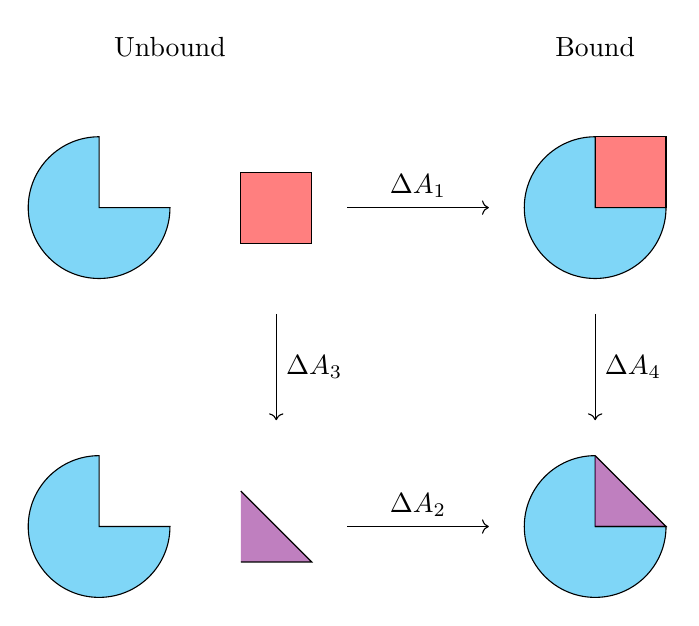
\begin{tikzpicture}[scale=0.9]
            \node at (1,2)[above]{Unbound};
            \node at (7,2)[above]{Bound};
            \draw[fill=cyan,fill opacity=0.5] (0,0)--(1,0) arc (0:-270:1) -- cycle;
            \draw[fill=red,fill opacity=0.5] (2,-0.5) rectangle (3,0.5);
            \draw[->] (3.5,0)--node[above]{\(\Delta A_1\)}(5.5,0);
            \begin{scope}[shift={(7,0)}]
                \draw[fill=cyan,fill opacity=0.5] (0,0)--(1,0) arc (0:-270:1) -- cycle;
                \draw[fill=red,fill opacity=0.5] (0,0) rectangle (1,1);
            \end{scope}
            \draw[->] (3.5,-4.5)--node[above]{\(\Delta A_2\)}(5.5,-4.5);
            \draw[->] (7,-1.5)--node[right]{\(\Delta A_4\)}(7,-3);
            \draw[->] (2.5,-1.5)--node[right]{\(\Delta A_3\)}(2.5,-3);
            \begin{scope}[shift={(0,-4.5)}]
                \draw[fill=cyan,fill opacity=0.5] (0,0)--(1,0) arc (0:-270:1) -- cycle;
                \draw[fill=violet,fill opacity=0.5] (2,-0.5) -- (3,-0.5) -- (2,0.5);
            \end{scope}
            \begin{scope}[shift={(7,-4.5)}]
                \draw[fill=cyan,fill opacity=0.5] (0,0)--(1,0) arc (0:-270:1) -- cycle;
                \draw[fill=violet,fill opacity=0.5] (0,0) -- (1,0) -- (0,1);
            \end{scope}
        \end{tikzpicture}
        \caption{Thermodynamic cycle calculating the relative binding affinities of two ligands with the same protein substrate.}
        \label{Fig:thermodynamic_cycle}
    \end{figure}








    \newpage
    \part*{Appendices}
    \addcontentsline{toc}{part}{\protect\numberline{}Appendices}
    \appendix

    \section{Noether's Theorem}\label{Appendix:Noether}
    The simplest way of deriving Noether's theorem is to use the Lagrangian mechanics, which is another way of formulating classical mechanics. First let's be clear of our notations. For a system of \(N\) particles in \(d\) dimensions, we will rewrite the coordinates \(\vb{r}_i\) as \(x^A\), where \(A=1,\dots,dN\). The Newton's equations are
    \begin{equation}\label{Newtons_eqn}
        \dot{p}_A=-\pdv{V}{x^A}\,,
    \end{equation}
    where \(p_A=m_A\dot{x}^A\). To reduce the clutter in notations, when we write \(x^A\) in the argument of a function, we mean that it is a function of all \(x^A\).
    
    Lagrangian mechanics starts from defining the Lagrangian of a system.
    \begin{defn}
        The \textit{Lagrangian} for a system is defined by
        \begin{equation}
            L(x^A,\dot{x}^A)=T(\dot{x}^A)-V(x^A)\,,
        \end{equation}
        where \(T=\frac{1}{2}\sum_{A}m_A(\dot{x}^A)^2\) is the kinetic energy and \(V(x^A)\) is the potential energy.
    \end{defn}
    Note the weird minus sign between the kinetic and the potential energy. Despite this strange definition of the Lagrangian, it works really elegantly.

    If we know that at \(t=t_0\), the particles are at \(x^A(t_0)=x^A_0\), and at \(t=t_1\), the particles are at \(x^A(t_1)=x^A_1\), there are infinite ways the systems can evolve with times between these two end points. How do we find the true paths \(x^A(t)\) taken by the particles?
    \begin{thm}[Principle of Least Action]
        The actual path taken by the system is an extremum of the \textit{action}, defined by
        \begin{equation}
            S[x^A(t)]=\int_{t_0}^{t_1}\dd{t}L(x^A(t),\dot{x}^A(t))\,.
        \end{equation}
    \end{thm}
    The \(S\) is an example of a \textit{functional}. It maps functions to a number.
    \begin{proof}
        Consider varying a given path slightly, so
        \begin{equation}
            x^A(t)\longrightarrow x^A(t)+\delta x^A(t)\,,
        \end{equation}
        where we fix the end points of the path by demanding \(\delta x^A(t_0)=\delta x^A(t_1)=0\). Then this results in a change in the action
        \begin{align}
            \delta S&=\delta\left[\int_{t_0}^{t_1}\dd{t}L\right]\notag\\
            &=\int_{t_0}^{t_1}\dd{t}\delta L\notag\\
            &=\int_{t_0}^{t_1}\dd{t}\sum_{A}\pdv{L}{x^A}\delta x^A+\pdv{L}{\dot{x}^A}\delta\dot{x}^A\,.
        \end{align}
        We integrate the second term by parts to get
        \begin{equation}
            \delta S=\int_{t_0}^{t_1}\dd{t}\sum_A\left[\pdv{L}{x^A}-\dv{}{t}\left(\pdv{L}{\dot{x}^A}\right)\right]\delta x^A + \left[\pdv{L}{\dot{x}^A}\delta x^A\right]_{t_0}^{t_1}\,.
        \end{equation}
        The boundary term vanishes since we required \(\delta x^A(t_0)=\delta x^A(t_1)=0\). At an extremum of the action \(S\), \(\delta S=0\) for all changes in the path \(\delta x^A(t)\). This holds if and only if
        \begin{equation}\label{Euler_Lagrange}
            \pdv{L}{x^A}-\dv{}{t}\left(\pdv{L}{\dot{x}^A}\right)=0\,.
        \end{equation}
        for all \(A\). These are known as the Euler--Lagrange equations. To finish the proof, we only need to show that Euler--Lagrange equations are equivalent to Newton's equations. From the definition of the Lagrangian, we have
        \begin{equation}
            \pdv{L}{x^A}=-\pdv{V}{x^A}\,,
        \end{equation}
        while
        \begin{equation}
            \pdv{L}{\dot{x}^A}=p_A\,.
        \end{equation}
        Then it's easy to see that Newton's equations (\ref{Newtons_eqn}) are indeed equivalent to Euler--Lagrange equations (\ref{Euler_Lagrange}).\qed
    \end{proof}

    In fact Lagrangian mechanics is much more powerful than that. It turns out we can use any generalised coordinate we want (e.g. spherical, hyperbolic, or just some arbitrary parameters that uniquely define the configuration of the system), and we may add constraints to the coordinates, making it much more powerful than Newton's formulation of classical mechanics. Unfortunately, we can't go into too much detail here. If you are interested, see e.g. Prof. David Tong's notes on \href{https://www.damtp.cam.ac.uk/user/tong/dynamics.html}{Classical Dynamics}. But the important conclusion is that for any Lagrangian written in generalised coordinates \(L(q_i,\dot{q}_i,t)\), the Euler--Lagrange equations still hold:
    \begin{equation}
        \pdv{L}{q_i}-\dv{}{t}\left(\pdv{L}{\dot{q}_i}\right)=0\,.
    \end{equation}

    \begin{defn}
        Consider a one-parameter transformation of maps
        \begin{equation}
            q_i(t)\longrightarrow Q_i(s,t)
        \end{equation}
        for \(s\in\RR\) such that \(Q_i(0,t)=q_i(t)\). Then this transformation is said to be a \textit{continuous symmetry} of the Lagrangian \(L\) if
        \begin{equation}
            \pdv{}{s}L(Q_i(s,t),\dot{Q}_i(s,t),t)=0\,.
        \end{equation}
    \end{defn}
    \begin{thm}[Noether's theorem]
        For each continuous symmetry, there is a conserved quantity.
    \end{thm}
    \begin{proof}
        \begin{equation}
            \pdv{L}{s}=\sum_i \pdv{L}{Q_i}\pdv{Q_i}{s}+\pdv{L}{\dot{Q}_i}\pdv{\dot{Q}_i}{s}\,,
        \end{equation}
        so we have
        \begin{align}
            0=\pdv{L}{s}\bigg|_{s=0}&=\sum_i\pdv{L}{q_i}\pdv{Q_i}{s}\bigg|_{s=0}+\pdv{L}{\dot{q}_i}\pdv{\dot{Q}_i}{s}\bigg|_{s=0}\notag\\
            &=\sum_i\dv{}{t}\left(\pdv{L}{\dot{q}_i}\right)\pdv{Q_i}{s}\bigg|_{s=0}+\pdv{L}{\dot{q}_i}\pdv{\dot{Q}_i}{s}\bigg|_{s=0}\notag \\
            &=\dv{}{t}\left(\sum_i\pdv{L}{\dot{q}_i}\pdv{Q_i}{s}\bigg|_{s=0}\right)\,.
        \end{align}
        The quantity
        \begin{equation}
            \sum_i\pdv{L}{\dot{q}_i}\pdv{Q_i}{s}\bigg|_{s=0}
        \end{equation}
        is constant for all time.\qed
    \end{proof}

    Let's find some examples.
    \begin{ex}
        \textit{Homogeneity of space}.

        Consider a system of \(N\) particles with Lagrangian
        \begin{equation}
            L=\frac{1}{2}\sum_i m_i\dot{\vb{r}_i}^2-V(r_{ij})\,,
        \end{equation}
        where \(V(r_{ij})\) means that the potential is only dependent on the relative distances \(r_{ij}=\norm{\vb{r}_i-\vb{r}_j}\) between particles, not on their absolute positions. Then this Lagrangian has symmetry of translation: \(\vb{r}_i\to\vb{r}_i+s\vb{n}\) for any vector \(\vb{n}\) and real number \(s\).
        \begin{equation}
            L(\vb{r}_i,\dot{\vb{r}}_i,t)=L(\vb{r}_i+s\vb{n},\dot{\vb{r}}_i,t)\,.
        \end{equation}
        Then by Noether's theorem, the conserved quantity is
        \begin{equation}
            \sum_i\pdv{L}{\dot{\vb{r}}_i}\vdot\vb{n}=\sum_i\vb{p}_i\vdot\vb{n}\,.
        \end{equation}
        The component of linear momentum in any direction is conserved, and hence
        \begin{equation}
            \sum_i\vb{p}_i
        \end{equation}
        is also conserved.

        Homogeneity in space \(\implies\) translational invariance of \(L\) \(\implies\) conservation of total linear momentum.
    \end{ex}
    \begin{ex}
        \textit{Isotropy of Space}.

        The isotropy of space means that a closed system is invariant under rotations around an axis \(\vu{n}\), so all \(\vb{r}_i\) are rotated to \(\vb{r}_i'\) by the same amount. To work out the corresponding conserved quantity it suffices to work with the infinitesimal form of the rotations
        \begin{equation}
            \vb{r}_i\longrightarrow \vb{r}_i+\delta\vb{r}_i=\vb{r}_i+\alpha\vu{n}\cross\vb{r}_i\,,
        \end{equation}
        where \(\alpha\) is infinitesimal. To see that this is indeed a rotation, you can calculate the length of the vector and notice it is preserved to linear order in \(\alpha\). Then we have
        \begin{equation}
            L(\vb{r}_i,\dot{\vb{r}}_i)=L(\vb{r}_i+\alpha\vu{n}\cross\vb{r}_i,\dot{r}_i+\alpha\vu{n}\cross\dot{\vb{r}}_i)\,,
        \end{equation}
        giving us the conserved quantity
        \begin{equation}
            \sum_i\pdv{L}{\dot{\vb{r}}_i}\vdot(\vu{n}\cross\vb{r}_i)=\sum_i\vu{n}\vdot(\vb{r}_i\cross\vb{p}_i)=\vu{n}\vdot\vb{L}\,.
        \end{equation}
        This is the component of the total angular momentum in the direction \(\vu{n}\). Since \(\vu{n}\) is arbitrary, \(\vb{L}\) is conserved.

        Isotropy of space \(\implies\) rotational invariance of \(L\) \(\implies\) conservation of total angular momentum.
    \end{ex}
    


\end{document}